% Generated deterministically by scripts/build_partial_epub3.py.
% Inclusion authority: alignment/UNITS.jsonl sha256=8ccdce17d2b77e683b550c8575872ea1ae0dbb6da11eae16eaea8f2b046c4113
% Accepted contiguous prefix: OLP-0001--OLP-0160 (160 units).
% First excluded unit: OLP-0161.
% This cumulative file contains every accepted source body inline.  It does
% not follow source driver imports and therefore cannot include pending units.
\documentclass[openany]{memoir}
\newcommand*{\olpath}{upstream}
\newcommand*{\ollangid}{nl}
\newcommand*{\ollanguage}{dutch}
\usepackage[T1]{fontenc}
\usepackage[utf8]{inputenc}
\usepackage{mathpazo}
\usepackage{helvet}
\usepackage{courier}
\linespread{1.05}
\setlength{\emergencystretch}{1em}
\input{upstream/sty/open-logic.sty}
\input{upstream/sty/open-logic-defer.sty}
\includeenv{editorial}
\problemsperchapter
\let\cleardoublepage\clearpage
\hypersetup{
  unicode=true,
  pdflang={nl-NL},
  pdftitle={The Open Logic Text --- gedeeltelijke Nederlandstalige editie (standaardregister)},
  pdfauthor={The Open Logic Project and credited contributors},
  pdfsubject={Gedeeltelijke reader met uitsluitend de geaccepteerde aaneengesloten prefix OLP-0001--OLP-0160},
  pdfkeywords={logica, verzamelingenleer, Nederlandse vertaling, gedeeltelijke editie}
}
\begin{document}
\begin{titlingpage}
\begin{raggedleft}
\HUGE\selectfont\bfseries\sffamily The Open Logic Text
\vskip 3ex
\normalfont\huge Gedeeltelijke Nederlandstalige editie\\
\Large standaardregister
\vskip 4ex
\large Geaccepteerde broneenheden OLP-0001--OLP-0160\\
2026-09-26
\end{raggedleft}
\vfill
\noindent Gebaseerd op het Open Logic Project. De tekst en broncode worden
beschikbaar gesteld onder Creative Commons Naamsvermelding 4.0 Internationaal.
\end{titlingpage}
\chapter*{Reikwijdte van deze gedeeltelijke editie}
\addcontentsline{toc}{chapter}{Reikwijdte van deze gedeeltelijke editie}
Deze editie bevat uitsluitend de 160 opeenvolgende,
in \texttt{alignment/UNITS.jsonl} geaccepteerde broneenheden OLP-0001--OLP-0160.
Broneenheid OLP-0161 en alle latere eenheden zijn niet opgenomen.
Een vertaalbestand dat al bestaat maar nog niet als geaccepteerd is gemarkeerd,
maakt uitdrukkelijk geen deel uit van deze editie. Het laatste hoofdstuk kan
daardoor inhoudelijk onvolledig zijn; dat is een eigenschap van deze begrensde
editie en geen claim dat het volledige Open Logic Text al vertaald is.
\chapter*{Status en verantwoording}
Dit is een gedeeltelijke bronuitgave: 160 van 722 broneenheden in twee Nederlandse registers. De volledige oorspronkelijke wiskundige inhoud van deze eenheden is behouden; de laatste hoofdstukgrens kan midden in een hoofdstuk vallen. Er is nog geen gepubliceerde PDF of EPUB. De aangeboden samengestelde LaTeX is inhoudelijk samengesteld en bytegewijs gecontroleerd, maar in deze uitgave niet gecompileerd. Een eerdere bouwpoging kon de gedeelde TeX-vergrendeling niet verkrijgen en startte geen TeX-proces. De termen “geaccepteerd” en “gecontroleerd” verwijzen naar de vastgelegde AI-productiecontroles, niet naar onafhankelijk deskundigenonderzoek.

Vertaling en eerdere controles: OpenAI Codex; de huidige eigenaar gebruikt GPT-5.6 Sol, Ultra effort. De exacte historische model- en inspanningsinstelling van ieder tekstgedeelte zijn nog niet afzonderlijk bewezen; de huidige instelling wordt daarom niet aan alle eerdere vertaalbytes toegeschreven. Bronselectie, verpakking en publicatiecontrole voor deze uitgave: OpenAI Codex — GPT-6 Astra, Ultra effort. Geen menselijke redactie of beoordeling wordt geclaimd.
\tableofcontents*

% BEGIN ACCEPTED UNIT OLP-0001 path=translations/nl-standard/content/open-logic-about.tex source-sha256=f1b7c863e4468c1638c459ae0132d2f0d7f1520f9a144a7e35d813a44cdcd3e1
\begingroup
\def\olfilename{OLP-0001}
\def\olfilepath{content/}
\hypertarget{unit-OLP-0001}{}
\typeout{PARTIAL-READER-UNIT OLP-0001}
% BEGIN ACCEPTED BODY OLP-0001 body-sha256=f1b7c863e4468c1638c459ae0132d2f0d7f1520f9a144a7e35d813a44cdcd3e1
\chapter*{Over het Open Logic Project}
\addcontentsline{toc}{chapter}{Over het Open Logic Project}


De \textit{Open Logic Text} is een opensourceleerboek dat gezamenlijk wordt
geschreven. Het behandelt formele metalogica en formele methoden en begint op
een niveau waarvoor een inleidende cursus formele logica als voorkennis wordt
verondersteld. Hoewel het boek bestemd is voor een niet-wiskundig publiek, in
het bijzonder voor studenten filosofie en informatica, is de behandeling
wiskundig nauwkeurig.

Enkele onderwerpen die al in de tekst staan, worden mogelijk nog niet volledig
behandeld, en veel paragrafen moeten nog grondig worden herzien. We zijn van plan
de tekst in de toekomst met meer onderwerpen uit te breiden. Ook zijn we van
plan de tekst uit te breiden met onder meer een woordenlijst, een
literatuurlijst, historische toelichtingen, afbeeldingen en betere uitleg,
evenals paragrafen die de relevantie van de resultaten voor filosofie,
informatica en wiskunde toelichten, en meer opgaven en voorbeelden. Vindt u een
fout of hebt u een suggestie,
\href{https://github.com/OpenLogicProject/OpenLogic/wiki/Contributing}{laat het projectteam dat dan weten}.

Het project werkt volgens de uitgangspunten van open source. De tekst is niet
alleen vrij beschikbaar; we stellen ook de LaTeX-broncode beschikbaar onder de
Creative Commons Naamsvermelding-licentie. Deze licentie geeft iedereen het
recht ons werk te downloaden, te gebruiken, te wijzigen, anders te ordenen,
om te zetten en opnieuw te verspreiden, mits de makers naar behoren worden
vermeld. Meer informatie vindt u op de website van het Open Logic Project:
\href{http://openlogicproject.org/}{openlogicproject.org}.
% END ACCEPTED BODY OLP-0001
\endgroup
% END ACCEPTED UNIT OLP-0001

% BEGIN ACCEPTED UNIT OLP-0002 path=translations/nl-standard/content/content.tex source-sha256=a626c4fe2f7fa7f5ed74cffef1f73a4e6b88bacecce5c6381b7582ab7a8cd4ee
\begingroup
\def\olfilename{OLP-0002}
\def\olfilepath{content/}
\hypertarget{unit-OLP-0002}{}
\typeout{PARTIAL-READER-UNIT OLP-0002}
% BEGIN ACCEPTED BODY OLP-0002 body-sha256=cc8322991404b12c737d1c59ae467e9f36ca9c7ef09063330baaf086ea7c7eee
% open-logic.tex
% compiles to produce complete text using open-logic-dev style



\clearpage

\begin{editorial}
Dit bestand laadt alle inhoud die in het Open Logic Project is opgenomen.
Wanneer redactionele opmerkingen zoals deze zichtbaar zijn, betekent dit dat
het bestand is gecompileerd zonder rekening te houden met de manier waarop het
materiaal wordt gepresenteerd. Als u dit kunt lezen, is het waarschijnlijk
\emph{niet raadzaam} om met deze pdf les te geven of eruit te studeren.

Het Open Logic Project biedt veel mogelijkheden om een tekst samen te
stellen die beter geschikt is voor onderwijs of zelfstudie. Standaard worden
bijvoorbeeld alle logische operatoren als primitief behandeld en worden in
bewijzen alle gevallen voor alle operatoren uitgewerkt. Het is echter veel beter
om enkele van die gevallen als opgaven over te laten. Ook is het Open Logic
Project nog in ontwikkeling. Om samenwerking en verbetering te bevorderen,
wordt materiaal ook opgenomen als het alleen nog in conceptvorm is of als er nog
opgaven in ontbreken, enzovoort. In een pdf die voor een cursus wordt
samengesteld, worden zulke paragrafen weggelaten.

Bekijk voor pdf's die beter geschikt zijn voor onderwijs en studie de
\href{http://builds.openlogicproject.org/}{voorbeeldcursussen op de
  OLP-website}. Om zelf een pdf samen te stellen, kunt u beginnen met het
\href{https://github.com/OpenLogicProject/OpenLogic/tree/master/courses/sample}{voorbeelddriverbestand}
of de bronbestanden van de afgeleide leerboeken raadplegen
voor uitgebreidere en geavanceerdere voorbeelden.
\end{editorial}
% END ACCEPTED BODY OLP-0002
\endgroup
% END ACCEPTED UNIT OLP-0002

% BEGIN ACCEPTED UNIT OLP-0003 path=translations/nl-standard/content/sets-functions-relations/sets-functions-relations-complete.tex source-sha256=a3713086170d2507be1c5f31616423ed74b4551fa4eab32201e40a5dcdadd9b6
\begingroup
\def\olfilename{OLP-0003}
\def\olfilepath{content/sets-functions-relations/}
\hypertarget{unit-OLP-0003}{}
\typeout{PARTIAL-READER-UNIT OLP-0003}
% BEGIN ACCEPTED BODY OLP-0003 body-sha256=97f7cf7cec9c45423f378d2df33f1a959b5278e03f8a711aae87f88049d2afcc
% Part: sets-functions-relations-complete



\olpart{sfr}{Na\"ieve verzamelingenleer}

\begin{editorial}
  Dit deel biedt een inleiding in de grondbeginselen van de naïeve
  verzamelingenleer. Doordat Tim Buttons Open Set Theory erin is opgenomen,
  behandelt dit deel ook de opbouw van getallenstelsels en oneindigheid. Die
  stof is niet vereist voor de logische delen van het OLP.
\end{editorial}
% END ACCEPTED BODY OLP-0003
\endgroup
% END ACCEPTED UNIT OLP-0003

% BEGIN ACCEPTED UNIT OLP-0004 path=translations/nl-standard/content/sets-functions-relations/sets/sets.tex source-sha256=1570952ea3b3213bccddf2749fb326c61837a24fc7bd0c76b4cbfbf583dd2e17
\begingroup
\def\olfilename{OLP-0004}
\def\olfilepath{content/sets-functions-relations/sets/}
\hypertarget{unit-OLP-0004}{}
\typeout{PARTIAL-READER-UNIT OLP-0004}
% BEGIN ACCEPTED BODY OLP-0004 body-sha256=ce20c644c2d2dc0b704c14d84be85697ade2cc27d9be712051664b5e681a50be
% Part: sets-functions-relations
% Chapter: sets



\olchapter{sfr}{set}{Verzamelingen}
% END ACCEPTED BODY OLP-0004
\endgroup
% END ACCEPTED UNIT OLP-0004

% BEGIN ACCEPTED UNIT OLP-0005 path=translations/nl-standard/content/sets-functions-relations/sets/basics.tex source-sha256=c292ad6a0f7e1c6a60175dbbf137d70c5b24368032f9eb97898589f98028e330
\begingroup
\def\olfilename{OLP-0005}
\def\olfilepath{content/sets-functions-relations/sets/}
\hypertarget{unit-OLP-0005}{}
\typeout{PARTIAL-READER-UNIT OLP-0005}
% BEGIN ACCEPTED BODY OLP-0005 body-sha256=0deb96309172fcb846a8fe346795a46b8a56288717ff4f56b3fa24f95d5c0d74
% Part: sets-functions-relations
% Chapter: sets
% Section: basics



\olfileid{sfr}{set}{bas}
\olsection{Extensionaliteit}

Een \emph{verzameling} is een geheel van objecten dat als één
object wordt beschouwd. De objecten waaruit de verzameling bestaat,
heten \emph{elementen} of \emph{leden} van de verzameling. Als $x$
!!a{element} van een verzameling~$A$ is, schrijven we $x \in A$; zo
niet, dan schrijven we $x \notin A$. De verzameling zonder
!!{element}s heet de \emph{lege} verzameling en wordt
aangeduid met~‘$\emptyset$’.

\begin{explain}
Het maakt niet uit hoe we de verzameling \emph{aangeven}, in welke
\emph{volgorde} we haar !!{element}s plaatsen of zelfs hoe
\emph{vaak} we haar !!{element}s meetellen. Alleen welke
!!{element}s ze bevat, is van belang. Dit leggen we vast in het
volgende beginsel.
\end{explain}

\begin{defn}[Extensionaliteit]
  Als $A$ en $B$ verzamelingen zijn, dan geldt $A = B$ dan en slechts
  dan als elk !!{element} van~$A$ ook !!a{element} van~$B$ is, en
  omgekeerd.
\end{defn}

Dankzij extensionaliteit kunnen we bepaalde notatie gebruiken. Zijn
$a_{1}$, \dots, $a_{n}$ objecten, dan is $\{a_{1}, \dots, a_{n}\}$ in
het algemeen \emph{de} verzameling waarvan $a_1, \ldots, a_n$ de
!!{element}s zijn. We benadrukken het woord ‘\emph{de}’, want uit
extensionaliteit volgt dat er maar \emph{één} zo'n verzameling kan
zijn. Uit extensionaliteit volgt bovendien:
  \[
    \{a, a, b\} = \{a, b\} = \{b,a\}.
  \] 
Dit weerspiegelt dat bij verzamelingen de volgorde van de
!!{element}s er niet toe doet, evenmin als het aantal keren dat ze
worden vermeld.

\begin{tagblock}{novice}
\begin{ex}
Elke groep objecten kan tot een verzameling worden samengenomen. De
verzameling van Richards broers en zussen bevat bijvoorbeeld één
persoon en kan worden geschreven als $S=\{\textrm{Ruth}\}$. De
verzameling van de positieve gehele getallen kleiner dan $4$ is
$\{1, 2, 3\}$, maar kan ook worden geschreven als $\{3, 2, 1\}$ of
zelfs als $\{1, 2, 1, 2, 3\}$. Volgens extensionaliteit zijn dit
allemaal dezelfde verzameling: elk !!{element} van $\{1, 2, 3\}$ is
ook !!a{element} van $\{3, 2, 1\}$ (en van $\{1, 2, 1, 2, 3\}$), en
omgekeerd.
\end{ex} 
\end{tagblock}

Vaak geven we een verzameling aan met een eigenschap die haar
!!{element}s gemeen hebben. Daarvoor gebruiken we de volgende verkorte
notatie: $\Setabs{x}{\phi(x)}$. Hier staat $\phi(x)$ voor de
eigenschap die~$x$ moet hebben om tot de !!{element}s van de
verzameling te worden gerekend.

\begin{tagblock}{novice}
\begin{ex}
In ons voorbeeld hadden we $S$ ook als volgt kunnen aangeven:
\[
S = \Setabs{x}{x \text{ een broer of zus van Richard is}}.
\]
\end{ex}
\end{tagblock}

\begin{tagblock}{math}
\begin{ex}
Een getal heet \emph{volmaakt} dan en slechts dan als het gelijk is
aan de som van zijn echte delers (d.w.z. getallen waardoor het zonder
rest deelbaar is, maar die niet gelijk zijn aan het getal zelf). Zo is
$6$ volmaakt, want zijn echte delers zijn $1$, $2$ en~$3$, en
$6 = 1 + 2 + 3$. Het getal $6$ is zelfs het enige positieve gehele
getal kleiner dan $10$ dat volmaakt is. Met extensionaliteit kunnen we
dus schrijven:
\[
	\{6\} = \Setabs{x}{x\text{ volmaakt is en }0 \leq x \leq 10}
\]
We lezen de notatie rechts als ‘de verzameling van alle $x$ waarvoor
$x$ volmaakt is en $0 \leq x \leq 10$’. Deze gelijkheid bevestigt dat
het bij verzamelingen niet uitmaakt hoe ze worden aangegeven. Meer in
het algemeen volgt uit extensionaliteit dat er hoogstens één verzameling
van alle $x$ kan zijn waarvoor $\phi(x)$ geldt. Daarom mogen we
$\Setabs{x}{\phi(x)}$ \emph{de} verzameling van alle $x$ noemen
waarvoor~$\phi(x)$ geldt.
\end{ex}
\end{tagblock}

Met extensionaliteit kunnen we aantonen dat verzamelingen gelijk zijn: om
$A = B$ te bewijzen, tonen we aan dat uit $x \in A$ steeds $x \in B$ volgt
en uit $y \in B$ steeds $y \in A$.

\begin{prob}
Bewijs dat er hoogstens één lege verzameling is, d.w.z. toon aan dat
als $A$ en $B$ verzamelingen zonder !!{element}s zijn, dan $A = B$.
\end{prob}
% END ACCEPTED BODY OLP-0005
\endgroup
% END ACCEPTED UNIT OLP-0005

% BEGIN ACCEPTED UNIT OLP-0006 path=translations/nl-standard/content/sets-functions-relations/sets/subsets.tex source-sha256=d37391ba1422c88024141b396853cc878fca33ed43c4521f892361e367f28205
\begingroup
\def\olfilename{OLP-0006}
\def\olfilepath{content/sets-functions-relations/sets/}
\hypertarget{unit-OLP-0006}{}
\typeout{PARTIAL-READER-UNIT OLP-0006}
% BEGIN ACCEPTED BODY OLP-0006 body-sha256=73cef67682c90286c44ee54bafdba96a8c3d8c49efcdf8bf2062a36b00768730
% Part: sets-functions-relations
% Chapter: sets
% Section: subsets



\olfileid{sfr}{set}{sub}
\olsection{Deelverzamelingen en machtsverzamelingen}

\begin{explain}
We zullen verzamelingen vaak met elkaar willen vergelijken. Een voor de
hand liggende vergelijking is: \emph{alles wat in de ene verzameling
zit, zit ook in de andere}. Deze situatie is belangrijk genoeg om er
nieuwe notatie voor in te voeren.
\end{explain}

\begin{defn}[Deelverzameling]
Als elk !!{element} van een verzameling $A$ ook !!a{element} van~$B$
is, noemen we $A$ een \emph{deelverzameling} van~$B$ en schrijven we
$A \subseteq B$. Als $A$ geen deelverzameling van~$B$ is, schrijven
we $A \not\subseteq B$. Als $A \subseteq B$ maar $A \neq B$, schrijven
we $A \subsetneq B$ en noemen we $A$ een \emph{echte
deelverzameling} van $B$.
\end{defn}

\begin{ex}
Elke verzameling is een deelverzameling van zichzelf, en $\emptyset$
is een deelverzameling van elke verzameling. De verzameling van de even
natuurlijke getallen is een deelverzameling van de verzameling van de
natuurlijke getallen. Ook geldt $\{ a, b \} \subseteq \{ a, b, c \}$.
Daarentegen is $\{ a, b, e \}$ geen deelverzameling van
$\{ a, b, c \}$.
\end{ex}

\begin{ex}
Het getal $2$ is een !!{element} van de verzameling van de gehele
getallen, terwijl de verzameling van de even getallen een
deelverzameling is van de verzameling van de gehele getallen. Een
verzameling kan echter \emph{zowel} !!a{element} als een deelverzameling van
een andere verzameling zijn. Zo geldt $\{0\} \in \{0, \{0\}\}$ en ook
$\{0\} \subseteq \{0, \{0\}\}$.
\end{ex}

Extensionaliteit geeft een gelijkheidscriterium voor verzamelingen:
$A = B$ dan en slechts dan als elk !!{element} van~$A$ ook
!!a{element} van~$B$ is, en omgekeerd. Volgens de definitie van
‘deelverzameling’ drukt $A \subseteq B$ precies de eerste helft van dit
criterium uit: elk !!{element} van~$A$ is ook !!a{element} van~$B$.
De definitie geldt uiteraard ook met $A$ en $B$ verwisseld: $B
\subseteq A$ dan en slechts dan als elk !!{element} van~$B$ ook
!!a{element} van~$A$ is. Dat is precies wat in extensionaliteit met ‘en
omgekeerd’ wordt bedoeld. Extensionaliteit impliceert dus dat
verzamelingen gelijk zijn dan en slechts dan als ze deelverzamelingen
van elkaar zijn.

\begin{prop}
$A = B$ dan en slechts dan als zowel $A \subseteq B$ als
$B \subseteq A$.
\end{prop}

Dit is ook een geschikt moment om nog enkele handige notaties in te
voeren. In de definitie van $A$ als deelverzameling van~$B$ schreven
we ‘elk !!{element} van~$A$ is \dots,’ en vulden we de ‘$\dots$’ aan
met ‘!!a{element} van $B$’. Uitdrukkingen met deze \emph{vorm} komen
zo vaak voor dat het nuttig is er formele notatie voor in te voeren.

\begin{defn}\ollabel{forallxina}
$(\forall x \in A)\phi$ is een afkorting voor $\forall x(x \in A \lif
\phi)$. Evenzo is $(\exists x \in A)\phi$ een afkorting voor $\exists
x(x \in A \land \phi)$.
\end{defn}

Met deze notatie kunnen we zeggen dat $A \subseteq B$ dan en slechts
dan als $(\forall x \in A)x \in B$.

We gaan nu over tot een bepaald soort verzameling: de verzameling van
alle deelverzamelingen van een gegeven verzameling.

\begin{defn}[Machtsverzameling]
De verzameling die uit alle deelverzamelingen van een verzameling~$A$
bestaat, heet de \emph{machtsverzameling van}~$A$ en wordt genoteerd
als $\Pow{A}$.
  \[
    \Pow{A} = \Setabs{B}{B \subseteq A} 
  \]
\end{defn}

\begin{ex}
Welke deelverzamelingen van $\{ a, b, c \}$ zijn er? Dit zijn:
$\emptyset$, $\{a \}$, $\{b\}$, $\{c\}$, $\{a, b\}$, $\{a, c\}$,
$\{b, c\}$ en $\{a, b, c\}$. De verzameling van al deze
deelverzamelingen is $\Pow{\{a,b,c\}}$:
\[
\Pow{\{ a, b, c \}} = \{\emptyset, \{a \}, \{b\}, \{c\}, \{a, b\},
\{b, c\}, \{a, c\}, \{a, b, c\}\}
\]
\end{ex}

\begin{prob}
Geef alle deelverzamelingen van $\{a, b, c, d\}$.
\end{prob}

\begin{prob}
Toon aan dat als $A$ uit $n$ !!{element}s bestaat, $\Pow{A}$ uit
$2^n$ !!{element}s bestaat.
\end{prob}
% END ACCEPTED BODY OLP-0006
\endgroup
% END ACCEPTED UNIT OLP-0006

% BEGIN ACCEPTED UNIT OLP-0007 path=translations/nl-standard/content/sets-functions-relations/sets/important-sets.tex source-sha256=0296704f72f34686d31b441aae1db555d0cbb9f6a7a8711f415140733fb1a60f
\begingroup
\def\olfilename{OLP-0007}
\def\olfilepath{content/sets-functions-relations/sets/}
\hypertarget{unit-OLP-0007}{}
\typeout{PARTIAL-READER-UNIT OLP-0007}
% BEGIN ACCEPTED BODY OLP-0007 body-sha256=6187068846147655ed73107c15aede34b96847337ee6c744a36c6674b6ad5c29
% Part: sets-functions-relations
% Chapter: sets
% Section: important-sets



\olfileid{sfr}{set}{imp}
\olsection{Enkele belangrijke verzamelingen}

\begin{ex}
We zullen voornamelijk verzamelingen behandelen waarvan de !!{element}en
wiskundige objecten zijn. Vier zulke verzamelingen zijn belangrijk genoeg
om een eigen naam te hebben:
\begin{multline*}
    \Nat = \{0, 1, 2, 3, \ldots\} \\
    \shoveright{\text{de verzameling natuurlijke getallen}}\\
    \shoveleft{\Int = \{\ldots, -2, -1, 0, 1, 2, \ldots\}} \\
    \shoveright{\text{de verzameling gehele getallen}}\\
    \shoveleft{\Rat = \Setabs{\nicefrac{m}{n}}{m, n \in \Int\text{ en }n \neq 0}}\\
    \shoveright{\text{de verzameling rationale getallen}}\\
    \shoveleft{\Real = (-\infty, \infty)}\\
    \text{de verzameling reële getallen (het continuüm)}
\end{multline*}
Dit zijn allemaal \emph{oneindige} verzamelingen: elk van deze verzamelingen
heeft oneindig veel !!{element}en.

Wanneer we deze verzamelingen in deze volgorde doorlopen, voegen we telkens
\emph{meer} getallen toe. De inclusies $\Nat \subseteq \Int
\subseteq \Rat \subseteq \Real$ liggen voor de hand: ieder natuurlijk
getal is immers een geheel getal, ieder geheel getal is rationaal en ieder
rationaal getal is reëel. Ook $\Nat \subsetneq \Int \subsetneq
\Rat$ is duidelijk, want $-1$ is wel een geheel maar geen natuurlijk getal,
en $\nicefrac{1}{2}$ is wel rationaal maar niet geheel. Minder duidelijk is
dat $\Rat \subsetneq \Real$, dus dat er reële getallen bestaan die niet
rationaal zijn\oliflabeldef{sfr:arith:real:realline}{; hierop komen we terug
in \olref[arith][real]{realline}}{}.

Soms gebruiken we ook de verzameling positieve gehele getallen $\PosInt = \{1,
2, 3, \dots\}$ en de verzameling die alleen de eerste twee natuurlijke
getallen bevat, $\Bin = \{0, 1\}$.
\end{ex}

\begin{tagblock}{compsci}
\begin{ex}[Tekenreeksen]
Een ander interessant voorbeeld is de verzameling $A^{*}$ van \emph{eindige
tekenreeksen} over een alfabet $A$: iedere eindige rij elementen van~$A$
is een tekenreeks over $A$. De \emph{lege tekenreeks $\Lambda$} rekenen we
tot de tekenreeksen over~$A$, voor elk alfabet~$A$. Bijvoorbeeld:
\begin{multline*}
\Bin^*
=\{\Lambda,0,1,00,01,10,11,\\
000,001,010,011,100,101,110,111,0000,\ldots\}.
\end{multline*}
Als $x=x_{1}\ldots x_{n}\in A^{*}$ een tekenreeks is die uit $n$
``letters'' van $A$ bestaat, dan heet~$n$ de \emph{lengte} van de tekenreeks
en schrijven we $\len{x}=n$.
\end{ex}
\end{tagblock}

\begin{ex}[Oneindige rijen]
Voor elke verzameling $A$ kunnen we ook de verzameling~$A^\omega$ van
oneindige rijen !!{element}en van~$A$ beschouwen. Een oneindige rij
$a_1a_2a_3a_4\dots$ bestaat uit een eenzijdig oneindige lijst van objecten,
die elk !!a{element} van~$A$ zijn.
\end{ex}
% END ACCEPTED BODY OLP-0007
\endgroup
% END ACCEPTED UNIT OLP-0007

% BEGIN ACCEPTED UNIT OLP-0008 path=translations/nl-standard/content/sets-functions-relations/sets/unions-and-intersections.tex source-sha256=f7978a32d97d329101142efaba5b9532f2bdc24dc88ade739a779a2ada57424e
\begingroup
\def\olfilename{OLP-0008}
\def\olfilepath{content/sets-functions-relations/sets/}
\hypertarget{unit-OLP-0008}{}
\typeout{PARTIAL-READER-UNIT OLP-0008}
% BEGIN ACCEPTED BODY OLP-0008 body-sha256=751a15ca7458869b9aae26c7c3de3161d3d835f4f5e2121eac5f710f26fb253a
% Part: sets-functions-relations
% Chapter: sets
% Section: unions-and-intersections



\olfileid{sfr}{set}{uni}
\olsection{Verenigingen en doorsneden}

\begin{explain}
In \olref[sfr][set][bas]{sec} hebben we verzamelingen door abstractie
gedefinieerd, dus met definities van de vorm $\Setabs{x}{\phi(x)}$.
Daarbij gebruiken we een eigenschap~$\phi$, waarin ook al gedefinieerde
verzamelingen mogen voorkomen. Zijn $A$ en~$B$ bijvoorbeeld verzamelingen,
dan bestaat $\Setabs{x}{x \in A \lor x \in B}$ uit alle objecten die
!!{element} zijn van $A$ of van~$B$. Deze verzameling verenigt dus de
!!{element}en van $A$ en~$B$. In \olref{fig:union} geeft het gemarkeerde
gebied de !!{element}en van de twee verzamelingen $A$ en~$B$ aan.

\begin{figure}
  \olasset{assets/diagrams/union.tikz}
  \caption{De vereniging $A \cup B$ van twee verzamelingen bestaat uit de
   !!{element}en van $A$ samen met die van~$B$.}
  \ollabel{fig:union} 
\end{figure}

Verzamelingen op deze manier verenigen is een veelgebruikte en nuttige
bewerking. Daarom geven we haar een formele naam en een symbool.
\end{explain}

\begin{defn}[Vereniging]
De \emph{vereniging} van twee verzamelingen $A$ en $B$, geschreven als
$A \cup B$, is de verzameling van alle objecten die !!{element} zijn van
$A$, van $B$ of van beide.
\[
A \cup B = \Setabs{x}{x \in A \lor x \in B}
\]
\end{defn}

\begin{ex}
Omdat herhaling van !!{element}en geen rol speelt, bevat de vereniging van
twee verzamelingen een gemeenschappelijk !!{element} maar één keer. Zo geldt
$\{ a, b, c\} \cup \{ a, 0, 1\} = \{a, b, c, 0, 1\}$.

De vereniging van een verzameling met een van haar deelverzamelingen is
de grotere verzameling: $\{a, b, c \} \cup \{a \} = \{a, b, c\}$.

De vereniging van een verzameling met de lege verzameling is die verzameling
zelf: $\{a, b, c \} \cup \emptyset = \{a, b, c \}$.
\end{ex}

\begin{prob}
Bewijs dat uit $A \subseteq B$ volgt dat $A \cup B = B$.
\end{prob}

\begin{explain}
We kunnen ook de ``duale'' bewerking van vereniging beschouwen. Deze bewerking
vormt de verzameling van alle !!{element}en die zowel !!{element} van~$A$
als !!{element} van~$B$ zijn. Zij heet \emph{doorsnede} en kan worden
weergegeven zoals in \olref{fig:intersection}.
\begin{figure}
  \olasset{assets/diagrams/intersection.tikz}
  \caption{De doorsnede $A \cap B$ van twee verzamelingen bestaat uit hun
    gemeenschappelijke !!{element}en.}
  \ollabel{fig:intersection}
\end{figure}
\end{explain}

\begin{defn}[Doorsnede]
De \emph{doorsnede} van twee verzamelingen $A$ en $B$, geschreven als
$A \cap B$, is de verzameling van alle objecten die zowel !!{element} van
$A$ als !!{element} van~$B$ zijn.
\[
A \cap B = \Setabs{x}{x \in A \land x \in B}
\]
Twee verzamelingen heten \emph{disjunct} als hun doorsnede leeg is. Ze hebben
dan geen !!{element}en gemeen.
\end{defn}

\begin{ex}
Als twee verzamelingen geen !!{element}en gemeen hebben, is hun doorsnede leeg:
$\{ a, b, c\} \cap \{ 0, 1\} = \emptyset$.

Als twee verzamelingen wel !!{element}en gemeen hebben, bestaat hun doorsnede
uit al die !!{element}en: $\{a, b, c \} \cap \{a, b, d \} = \{a, b\}$.

De doorsnede van een verzameling met een van haar deelverzamelingen is de
kleinere verzameling: $\{a, b, c\} \cap \{a, b\} = \{a, b\}$.

De doorsnede van elke verzameling met de lege verzameling is leeg: $\{a, b, c \}
\cap \emptyset = \emptyset$.
\end{ex}

\begin{prob}
Geef een rigoureus bewijs dat uit $A \subseteq B$ volgt dat $A \cap B = A$.
\end{prob}

\begin{explain}
We kunnen ook de vereniging of doorsnede van meer dan twee verzamelingen
vormen. Een elegante algemene aanpak is de volgende. Breng alle verzamelingen
waarvan we de vereniging of doorsnede willen nemen onder in één verzameling.
De vereniging van de oorspronkelijke verzamelingen is dan de verzameling van
alle objecten die tot ten minste één !!{element} van die verzameling behoren;
hun doorsnede is de verzameling van alle objecten die tot elk !!{element}
ervan behoren.
\end{explain}

\begin{defn}
Als $A$ een verzameling van verzamelingen is, dan is $\bigcup A$ de verzameling
van de !!{element}en van de !!{element}en van~$A$:
\begin{align*}
\bigcup A & = \Setabs{x}{x \text{ behoort tot !!a{element} van } A},
\text{ d.w.z.:}\\
& = \Setabs{x}{\text{er is een } B \in A
  \text{ waarvoor } x \in B}
\end{align*}
\end{defn}

\begin{defn}
Als $A$ een verzameling van verzamelingen is, dan is $\bigcap A$ de verzameling
van de objecten die alle elementen van~$A$ gemeen hebben:
\begin{align*}
\bigcap A & = \Setabs{x}{x \text{ behoort tot elk !!{element} van } A},
\text{ d.w.z.:}\\
 & = \Setabs{x}{\text{voor elke } B \in A, x \in B}
\end{align*}
\end{defn}

\begin{ex}
Stel $A = \{ \{ a, b \}, \{ a, d, e \}, \{ a, d \} \}$.
Dan is $\bigcup A = \{ a, b, d, e \}$ en $\bigcap A = \{ a \}$.
\end{ex}
\begin{prob}
	Toon aan dat als $A$ een verzameling is en $A \in B$, dan
	$A \subseteq \bigcup B$.
\end{prob}

Hetzelfde kan voor een rij verzamelingen $A_1$, $A_2$, \dots
\begin{align*}
\bigcup_i A_i & = \Setabs{x}{x \text{ behoort tot ten minste één van de } A_i}\\
\bigcap_i A_i & = \Setabs{x}{x \text{ behoort tot elk van de } A_i}.
\end{align*}

Als we een \emph{indexverzameling} $I$ hebben en verzamelingen $A_i$
beschouwen, één voor elke $i \in I$, kunnen we ook deze afkortingen gebruiken:
\begin{align*}
	\bigcup_{i \in I} A_i & = \bigcup \Setabs{A_i }{i \in I}\\
	\bigcap_{i \in I} A_i & = \bigcap\Setabs{A_i}{i \in I}
\end{align*}

Ten slotte kunnen we de verzameling van alle !!{element}en van~$A$ beschouwen
die niet in~$B$ liggen. Dit is weergegeven in \olref{difference}.

\begin{figure}
  \olasset{assets/diagrams/difference.tikz}
  \caption{Het verschil $A \setminus B$ van twee verzamelingen bestaat uit
    de !!{element}en van~$A$ die geen !!{element} van~$B$ zijn.}
  \ollabel{difference}
\end{figure}

\begin{defn}[Verschil]
Het \emph{verschil}~$A \setminus B$ is de verzameling van alle !!{element}en
van $A$ die geen !!{element} van~$B$ zijn, dus
\[
A\setminus B = \Setabs{x}{x\in A \text{ en } x \notin B}.
\]
\end{defn}

\begin{prob}
	Bewijs dat uit $A \subsetneq B$ volgt dat $B \setminus A \neq \emptyset$.
\end{prob}
% END ACCEPTED BODY OLP-0008
\endgroup
% END ACCEPTED UNIT OLP-0008

% BEGIN ACCEPTED UNIT OLP-0009 path=translations/nl-standard/content/sets-functions-relations/sets/pairs-and-products.tex source-sha256=ac1f714a0f0f5d0db3b83a47468d724d4f2e4c61774e22a5bff458e2b7fba792
\begingroup
\def\olfilename{OLP-0009}
\def\olfilepath{content/sets-functions-relations/sets/}
\hypertarget{unit-OLP-0009}{}
\typeout{PARTIAL-READER-UNIT OLP-0009}
% BEGIN ACCEPTED BODY OLP-0009 body-sha256=f4d251fdc35aac65ba3240439017561f19a6fe866ae3555158aa021c6ec699d0
% Part: sets-functions-relations
% Chapter: sets
% Section: pairs-and-products



\olfileid{sfr}{set}{pai}
\olsection{Paren, n-tallen en cartesische producten}

\begin{explain}
Uit extensionaliteit volgt dat de elementen van een verzameling geen
volgorde hebben. Om een volgorde weer te geven gebruiken we daarom
\emph{geordende paren} $\tuple{x, y}$. In een ongeordend paar $\{x,
y\}$ doet de volgorde er niet toe: $\{x, y\} = \{y, x\}$. In een
geordend paar is de volgorde wel van belang: als $x \neq y$, dan
$\tuple{x, y} \neq \tuple{y, x}$.

Hoe moeten we geordende paren in de verzamelingenleer opvatten?
Van wezenlijk belang is dat twee geordende paren dan en slechts dan gelijk
zijn als hun eerste elementen gelijk zijn en ook hun tweede elementen
gelijk zijn, dus:
\[
  \tuple{a, b}= \tuple{c, d}\text{ dan en slechts dan als zowel }a = c \text{ als }b=d.
\]
We kunnen geordende paren in de verzamelingenleer definiëren met de
definitie van Wiener--Kuratowski.
\end{explain}

\begin{defn}[Geordend paar]\ollabel{wienerkuratowski}
	$\tuple{a, b} = \{\{a\}, \{a, b\}\}$.
\end{defn}

\begin{prob}
	Bewijs met \olref[sfr][set][pai]{wienerkuratowski} dat $\tuple{a,
	b}= \tuple{c, d}$ dan en slechts dan als zowel $a = c$ als $b=d$.
\end{prob}

\begin{explain}
Nu we een definitie van een geordend paar hebben vastgelegd, kunnen we
daarmee andere verzamelingen definiëren. Soms hebben we bijvoorbeeld
ook geordende rijtjes van meer dan twee objecten nodig, zoals
\emph{drietallen} $\tuple{x, y, z}$, \emph{viertallen} $\tuple{x, y,
z, u}$, enzovoort. We kunnen drietallen opvatten als bijzondere
geordende paren waarvan het eerste element zelf een geordend paar is:
$\tuple{x, y, z}$ is $\tuple{\tuple{x, y},z}$. Hetzelfde geldt voor
viertallen: $\tuple{x,y,z,u}$ is
$\tuple{\tuple{\tuple{x,y},z},u}$, enzovoort. In het algemeen spreken
we van \emph{geordende $n$-tallen} $\tuple{x_1, \dots, x_n}$.

Bepaalde verzamelingen van geordende paren of andere geordende
$n$-tallen zullen van pas komen.
\end{explain}

\begin{defn}[Cartesisch product]
Gegeven verzamelingen $A$ en $B$ is hun \emph{cartesisch product} $A
\times B$ gedefinieerd door
\[
  A \times B = \Setabs{\tuple{x, y}}{x \in A \text{ en } y \in B}.
\]
\end{defn}

\begin{ex}
Als $A = \{0, 1\}$ en $B = \{1, a, b\}$, dan is hun product
\[
A \times B = \{ \tuple{0, 1}, \tuple{0, a}, \tuple{0, b},
    \tuple{1, 1}, \tuple{1, a}, \tuple{1, b} \}.
\]
\end{ex}

\begin{ex}
Als $A$ een verzameling is, schrijven we het product van $A$ met
zichzelf, $A \times A$, ook als~$A^2$. Dit is de verzameling van
\emph{alle} paren $\tuple{x, y}$ waarvoor $x, y \in A$. De
verzameling van alle drietallen $\tuple{x, y, z}$ is $A^3$,
enzovoort. We kunnen dit recursief definiëren:
\begin{align*}
  A^1 & = A\\
  A^{k+1} & = A^k \times A
\end{align*}
\end{ex}

\begin{prob}
Geef alle !!{element}s van $\{1, 2, 3\}^3$.
\end{prob}

\begin{prop}\ollabel{cardnmprod}
Als $A$ uit $n$ !!{element}s bestaat en $B$ uit $m$ !!{element}s, dan
heeft $A \times B$ precies $n\cdot m$ elementen.
\end{prop}

\begin{proof}
Voor elk !!{element}~$x$ van~$A$ zijn er $m$ !!{element}s van de vorm
$\tuple{x, y} \in A \times B$. Laat $B_x = \Setabs{\tuple{x, y}}{y
  \in B}$. Als $x_1 \neq x_2$, verschilt elk paar uit de ene zo
gevormde verzameling van elk paar uit de andere; in het bijzonder geldt $\tuple{x_1, y} \neq
\tuple{x_2, y}$. Daarom is $B_{x_1} \cap B_{x_2} = \emptyset$. Als
$A = \{x_1, \dots, x_n\}$, dan is bovendien $A \times B = B_{x_1}
\cup \dots \cup B_{x_n}$ en heeft dit product dus $n\cdot m$
!!{element}s.

We kunnen dit weergeven door de !!{element}s van~$A \times B$ in een
rooster te zetten:
\[
\begin{array}{rcccc}
  B_{x_1} = & \{\tuple{x_1, y_1} & \tuple{x_1, y_2} & \dots & \tuple{x_1, y_m}\}\\
  B_{x_2} = & \{\tuple{x_2, y_1} & \tuple{x_2, y_2} & \dots & \tuple{x_2, y_m}\}\\
  \vdots & & \vdots\\
  B_{x_n} = & \{\tuple{x_n, y_1} & \tuple{x_n, y_2} & \dots & \tuple{x_n, y_m}\}
\end{array}
\]
Omdat alle $x_i$ onderling verschillend zijn en ook alle $y_j$
onderling verschillend zijn, zijn geen twee paren in dit rooster
gelijk. Er staan er $n\cdot m$ in.
\end{proof}

\begin{prob}
Bewijs met inductie naar~$k$ dat voor alle $k \ge 1$ geldt: als $A$
$n$ !!{element}s heeft, dan heeft $A^k$ precies $n^k$ !!{element}s.
\end{prob}

\begin{ex}
Als $A$ een verzameling is, is een \emph{woord} over~$A$ een
willekeurig rijtje !!{element}s van~$A$. Een rijtje kan worden opgevat
als een geordend $n$-tal van !!{element}s van~$A$. Als bijvoorbeeld $A =
\{a, b, c\}$, dan kan het rijtje ‘$bac$’ worden opgevat als het
drietal~$\tuple{b, a, c}$. Woorden, dat wil zeggen rijtjes symbolen,
zijn van wezenlijk belang in de informatica. Volgens afspraak
beschouwen we !!{element}s van~$A$ als rijtjes van lengte~$1$, en
$\emptyset$ als het rijtje van lengte~$0$. De verzameling van
\emph{alle} woorden over~$A$ is dan
\[
A^* = \{\emptyset\} \cup A \cup A^2 \cup A^3 \cup \dots
\]
\end{ex}
% END ACCEPTED BODY OLP-0009
\endgroup
% END ACCEPTED UNIT OLP-0009

% BEGIN ACCEPTED UNIT OLP-0010 path=translations/nl-standard/content/sets-functions-relations/sets/russells-paradox.tex source-sha256=11855f7fc2342353f89cd0b2c18af5a331d2edbdf52607c49577737a370181e7
\begingroup
\def\olfilename{OLP-0010}
\def\olfilepath{content/sets-functions-relations/sets/}
\hypertarget{unit-OLP-0010}{}
\typeout{PARTIAL-READER-UNIT OLP-0010}
% BEGIN ACCEPTED BODY OLP-0010 body-sha256=cab4b6d66a4ea42de3bff4ae0b0559ad3fe1f4aa4a538985cba8d940c0e55b6d
% Part: sets-functions-relations
% Chapter: sets
% Section: russells-paradox




\olfileid{sfr}{set}{rus}
\olsection{De paradox van Russell}

Op grond van extensionaliteit mogen we de notatie
$\Setabs{x}{\phi(x)}$ gebruiken voor \emph{de} verzameling van alle
$x$ waarvoor~$\phi(x)$ geldt. Uit extensionaliteit volgt echter
\emph{werkelijk} alleen het volgende. \emph{Als} er een verzameling
bestaat met precies de objecten die aan~$\phi$ voldoen als elementen,
\emph{dan} is er maar één zo'n verzameling. Anders gezegd: als~$\phi$
is vastgelegd, is de verzameling
$\Setabs{x}{\phi(x)}$ uniek, \emph{als zij bestaat}.

Maar dit voorbehoud is belangrijk!{} Niet iedere eigenschap leent
zich voor \emph{comprehensie}. Sommige eigenschappen definiëren dus
\emph{geen} verzameling. Als alle eigenschappen dat wel deden, zouden
we regelrecht in tegenspraken belanden. Het bekendste voorbeeld
hiervan is de paradox van Russell.

Verzamelingen kunnen !!{element}s van andere verzamelingen zijn---de
machtsverzameling van een verzameling~$A$ bestaat bijvoorbeeld zelf
uit verzamelingen. Daarom is het zinvol na te gaan of een verzameling
!!a{element} van een andere verzameling is. Kan een verzameling
element van zichzelf zijn? Het begrip verzameling lijkt dat niet uit
te sluiten. Als \emph{alle} verzamelingen bijvoorbeeld samen een
collectie objecten vormen, zou men kunnen denken dat ze in één
verzameling kunnen worden samengebracht---de verzameling van alle
verzamelingen. Omdat die zelf een verzameling is, zou zij
!!a{element} van de verzameling van alle verzamelingen zijn.

De paradox van Russell ontstaat wanneer we de eigenschap beschouwen
om zichzelf niet als !!a{element} te hebben, oftewel \emph{geen
element van zichzelf te zijn}. Stel dat er een verzameling bestaat
van alle verzamelingen die zichzelf niet als !!a{element} hebben.
Bestaat
\[
R = \Setabs{x}{x \notin x}
\]
dan? We kunnen bewijzen dat dit niet zo is.

\begin{thm}[De paradox van Russell]\ollabel{thm:russells-paradox}
	Er bestaat geen verzameling $R = \Setabs{x}{x \notin x}$.
\end{thm}

\begin{proof}
Als $R = \Setabs{x}{x \notin x}$ bestaat, dan geldt
$R \in R$ dan en slechts dan als $R \notin R$. Dat is een tegenspraak.
\end{proof}

\begin{tagblock}{novice}
\begin{explain}
Laten we dit bewijs langzamer doorlopen. Als $R$ bestaat, is het
zinvol te vragen of $R \in R$ geldt. Neem eerst aan dat inderdaad $R
\in R$. De verzameling~$R$ is gedefinieerd als de verzameling van alle
verzamelingen die geen !!{element}s van zichzelf zijn. Als $R \in R$,
dan is $R$ element van zichzelf en mist die verzameling dus de eigenschap
waarmee $R$ is gedefinieerd. Maar alleen verzamelingen met die eigenschap
behoren tot~$R$. Daarom kan $R$ geen !!{element} van~$R$ zijn, dus
$R \notin R$. De verzameling~$R$ kan niet zowel wel als niet
!!a{element} van~$R$ zijn. We hebben dus een tegenspraak.

Omdat de aanname $R \in R$ tot een tegenspraak leidt, volgt $R \notin
R$. Maar ook dit leidt tot een tegenspraak!{} Want als $R \notin R$,
dan heeft $R$ zelf juist wel de eigenschap waarmee $R$ is
gedefinieerd. Net als alle andere verzamelingen die geen element van
zichzelf zijn, zou $R$ dus !!a{element} van $R$ zijn. Opnieuw kan $R$
niet zowel geen als wel !!a{element} van zichzelf zijn.
\end{explain}
\end{tagblock}

\begin{digress}
Hoe kunnen we een verzamelingenleer opzetten zonder in de paradox van
Russell terecht te komen, dus zonder de \emph{inconsistente} bewering
te doen dat $R = \Setabs{x}{x \notin x}$ bestaat? Daarvoor moeten we
axioma's formuleren die heel precies aangeven wanneer verzamelingen
bestaan (en wanneer niet).
	
De verzamelingenleer die in dit hoofdstuk wordt geschetst doet dat
niet. Ze is \emph{werkelijk na\"ief}. Ze stelt alleen dat
verzamelingen aan extensionaliteit voldoen en dat we uit gegeven
verzamelingen hun vereniging, doorsnede enzovoort kunnen vormen. Het
is mogelijk de verzamelingenleer nauwkeuriger en strenger te ontwikkelen.
\oliflabeldef{cumul:::part}{Die strengere uitwerking komt aan bod in
Deel \olref[cumul][][]{part}. Voorlopig gaan we na\"ief verder en
proberen we tegenspraken zorgvuldig te vermijden.}{}
\end{digress}
% END ACCEPTED BODY OLP-0010
\endgroup
% END ACCEPTED UNIT OLP-0010
\OLEndChapterHook

% BEGIN ACCEPTED UNIT OLP-0011 path=translations/nl-standard/content/sets-functions-relations/relations/relations-complete.tex source-sha256=448341fbb5ffdee88215b9a4cf91a831e2f3befd11e38cbfd969d4fe394e1dd8
\begingroup
\def\olfilename{OLP-0011}
\def\olfilepath{content/sets-functions-relations/relations/}
\hypertarget{unit-OLP-0011}{}
\typeout{PARTIAL-READER-UNIT OLP-0011}
% BEGIN ACCEPTED BODY OLP-0011 body-sha256=ef62c92774115ecbd7113ee0f2cd5e683420f8075e50c123ceace1f6fe6de4c7
% Part: sets-functions-relations
% Chapter: relations-complete



\olchapter{sfr}{rel}{Relaties}
% END ACCEPTED BODY OLP-0011
\endgroup
% END ACCEPTED UNIT OLP-0011

% BEGIN ACCEPTED UNIT OLP-0012 path=translations/nl-standard/content/sets-functions-relations/relations/relations-as-sets.tex source-sha256=0377b2beaa32ad8d9bf5a068e1b9edb7595d802285506e52eff4a9c4dc67d346
\begingroup
\def\olfilename{OLP-0012}
\def\olfilepath{content/sets-functions-relations/relations/}
\hypertarget{unit-OLP-0012}{}
\typeout{PARTIAL-READER-UNIT OLP-0012}
% BEGIN ACCEPTED BODY OLP-0012 body-sha256=a2eb57508f05aed1c05027e2fcb290a7b1ad8a42b00e27bad1908cf090518748
% Part: sets-functions-relations
% Chapter: relations
% Section: relations-as-sets



\olfileid{sfr}{rel}{set}
\olsection{Relaties als verzamelingen}

\begin{explain}
In \olref[sfr][set][imp]{sec} hebben we enkele belangrijke
verzamelingen genoemd: $\Nat$, $\Int$, $\Rat$, $\Real$. U herinnert
zich ongetwijfeld nog enkele interessante relaties tussen de !!{element}s
van sommige van deze verzamelingen. Zo heeft elk ervan een gebruikelijke
\emph{ordening}. Daarnaast is er de \emph{identiteit}, die ieder object
met zichzelf en met geen enkel ander object verbindt. We zullen nog veel meer
interessante relaties tegenkomen, en er zijn nog meer relaties mogelijk.
Voordat we die bespreken, merken we echter eerst op dat een relatie als een
bijzonder soort verzameling kan worden opgevat.
  
Hiervoor hebben we twee begrippen uit \olref[sfr][set][pai]{sec} nodig.
Ten eerste is er het \emph{geordende paar}: uit $a$ en $b$ kunnen
we~$\tuple{a, b}$ vormen. De volgorde van de elementen is hier
\emph{wel} van belang. Als $a \neq b$, dan is dus $\tuple{a, b} \neq
\tuple{b, a}$. (Bij ongeordende paren, dat wil zeggen verzamelingen met
$2$ elementen, geldt daarentegen $\{a, b\}=\{b, a\}$.) Ten tweede is er het
\emph{cartesisch product}: als $A$ en $B$ verzamelingen zijn, kunnen we
$A \times B$ vormen, de verzameling van alle paren $\tuple{x, y}$ met
$x \in A$ en $y \in B$. In het bijzonder is $A^{2}= A \times A$ de
verzameling van alle geordende paren uit~$A$.
  
We beschouwen nu één bepaalde relatie op een verzameling: de
$<$-relatie op de verzameling~$\Nat$ van natuurlijke getallen. Neem de
verzameling van alle getallenparen $\tuple{n, m}$ waarvoor $n<m$, dus
\[
  R=\Setabs{\tuple{n, m}}{n, m \in \Nat \text{ en } n<m}.
\]
Dat $n$ kleiner is dan $m$, komt precies overeen met het feit dat het
paar $\tuple{n, m}$ tot $R$ behoort:
\[
      n<m\text{ desda }\tuple{n, m} \in R.
\]
We kunnen de verzameling $R$ dan ook zonder informatieverlies
\emph{opvatten als} de $<$-relatie op $\Nat$.

Op dezelfde manier kunnen we voor iedere relatie tussen getallen een
deelverzameling van $\Nat^{2}$ construeren. Omgekeerd bepaalt iedere
verzameling getallenparen $S \subseteq \Nat^{2}$ een bijbehorende
relatie tussen getallen, namelijk de relatie waarin $n$ tot $m$ staat
desda $\tuple{n, m} \in S$. Dit rechtvaardigt de volgende definitie:
\end{explain}
  
\begin{defn}[Binaire relatie]
Een \emph{binaire relatie} op een verzameling $A$ is een
deelverzameling van~$A^{2}$. Als $R \subseteq A^{2}$ een binaire
relatie op~$A$ is en $x, y \in A$, schrijven we soms $Rxy$ (of $xRy$)
voor $\tuple{x, y} \in R$.
\end{defn}
  
\begin{ex}
  \ollabel{relations}
De verzameling $\Nat^{2}$ van paren natuurlijke getallen kan als volgt
in een tweedimensionale matrix worden weergegeven:
\[
  \begin{array}{ccccc}
  \mathbf{\tuple{ 0,0 }} & \tuple{ 0,1 } &
    \tuple{ 0,2 } & \tuple{ 0,3 } & \ldots\\
  \tuple{ 1,0 } & \mathbf{\tuple{ 1,1 }} &
    \tuple{ 1,2 } & \tuple{ 1,3 } & \ldots\\
  \tuple{ 2,0 } & \tuple{ 2,1 } &
    \mathbf{\tuple{ 2,2 }} & \tuple{ 2,3 } & \ldots\\
  \tuple{ 3,0 } & \tuple{ 3,1 } & \tuple{ 3,2 } &
    \mathbf{\tuple{ 3,3 }} & \ldots\\
  \vdots & \vdots & \vdots & \vdots & \mathbf{\ddots}
  \end{array}
\]
De diagonaal is hier vet gedrukt, want de deelverzameling van $\Nat^2$
die bestaat uit de paren op de diagonaal, namelijk
\[
  \{\tuple{0,0 }, \tuple{ 1,1 }, \tuple{ 2,2 }, \dots\},
  \]
is de \emph{identiteit op}~$\Nat$. (Omdat de identiteit vaak wordt
gebruikt, definiëren we $\Id{A}=\Setabs{\tuple{ x,x }}{x \in A}$ voor
iedere verzameling $A$.) De deelverzameling van alle paren boven de
diagonaal, namelijk
\[
  L = \{\tuple{ 0,1 },\tuple{ 0,2 },\ldots,\tuple{ 1,2 },
  \tuple{ 1,3 }, \dots, \tuple{ 2,3 }, \tuple{ 2,4 },\ldots\},
\]
is de relatie \emph{kleiner dan}, dus $Lnm$ desda $n<m$. De
deelverzameling van alle paren onder de diagonaal, namelijk
\[
  G=\{ \tuple{ 1,0 },\tuple{ 2,0 },\tuple{
    2,1 }, \tuple{ 3,0 },\tuple{ 3,1 },\tuple{ 3,2 }, \dots\},
\]
is de relatie \emph{groter dan}, dus $Gnm$ desda $n>m$. De vereniging
van $L$ met de zojuist gedefinieerde identiteit~$I$, die we $K=L\cup I$
kunnen noemen, is de relatie
\emph{kleiner dan of gelijk aan}: $Knm$ desda $n \le m$. Evenzo is
$H=G \cup I$ de relatie \emph{groter dan of gelijk aan.} De relaties
$L$, $G$, $K$ en $H$ zijn bijzondere relaties die \emph{ordeningen}
heten. $L$ en $G$ hebben de eigenschap dat noch $L$, noch $G$ een getal
met zichzelf in verband brengt (voor alle $n$ geldt dus noch $Lnn$,
noch $Gnn$). Relaties met deze eigenschap heten \emph{irreflexief};
zijn ze bovendien ordeningen, dan heten ze \emph{strikte ordeningen.}
\end{ex}

\begin{explain}
Hoewel ordeningen en de identiteit belangrijke, natuurlijke relaties
zijn, benadrukken we dat volgens onze definitie \emph{iedere}
deelverzameling van $A^{2}$ een relatie op~$A$ is, hoe onnatuurlijk of
gekunsteld die ook lijkt. Zo is $\emptyset$ een relatie op iedere
verzameling (de \emph{lege relatie}, die voor geen enkel elementenpaar
geldt), en is ook $A^{2}$~zelf een relatie op~$A$ (een relatie die voor
ieder paar geldt), de \emph{universele relatie}. Ook iets als
$E=\Setabs{\tuple{n, m}}{n>5 \text{ of } m \times n \ge 34}$ geldt als
een relatie.
\end{explain}
  
\begin{prob}
  Geef de !!{element}s van de relatie $\subseteq$ op de verzameling
  $\Pow{\{a, b, c\}}$.
\end{prob}
% END ACCEPTED BODY OLP-0012
\endgroup
% END ACCEPTED UNIT OLP-0012

% BEGIN ACCEPTED UNIT OLP-0013 path=translations/nl-standard/content/sets-functions-relations/relations/reflections.tex source-sha256=6c93d47101027efc1af4562501ab539e40afaebc7af369fd9401d3b9a0e1932d
\begingroup
\def\olfilename{OLP-0013}
\def\olfilepath{content/sets-functions-relations/relations/}
\hypertarget{unit-OLP-0013}{}
\typeout{PARTIAL-READER-UNIT OLP-0013}
% BEGIN ACCEPTED BODY OLP-0013 body-sha256=68cc5ced448f47f155d8491db8e715f9e4827ab755ff800c9e55bff64b67af95
% Part: sets-functions-relations
% Chapter: relations
% Section: reflections
%


\olfileid{sfr}{rel}{ref}
\olsection{Filosofische beschouwingen}

In \olref[set]{sec} hebben we relaties gedefinieerd als bepaalde
verzamelingen. Het is goed om even stil te staan bij een filosofische
vraag: wat \emph{doet} zo'n definitie? Het is zeer de vraag of we
willen zeggen dat we daarmee hebben \emph{ontdekt} welke dingen
metafysisch gezien identiek zijn; bijvoorbeeld dat de ordeningsrelatie op $\Nat$
\emph{bleek} samen te vallen met de verzameling $R=
\Setabs{\tuple{n,m}}{n, m \in \Nat\text{ en } n < m}$ die we in
\olref[set]{sec} hebben gedefinieerd. Daarvoor zijn drie redenen.

Ten eerste hebben we in \olref[set][pai]{wienerkuratowski} gedefinieerd
dat $\tuple{a, b} = \{\{a\}, \{a, b\}\}$. Beschouw in plaats daarvan de
definitie $\lVert a, b\rVert = \{\{b\}, \{a, b\}\} = \tuple{b,a}$. Als
$a \neq b$, dan geldt $\tuple{a, b} \neq \lVert a,b\rVert$. We hadden
echter net zo goed $\lVert a,b\rVert$ in plaats van $\tuple{a,b}$ als
definitie van een geordend paar kunnen kiezen. Beide definities zouden
even goed hebben gewerkt. Er zijn dus twee even geschikte
verzamelingen die als de ordeningsrelatie op de natuurlijke getallen
zouden kunnen gelden:
\begin{align*}
		R &= \Setabs{\tuple{n,m}}{n, m \in \Nat \text{ en }n < m}\\
		S &= \Setabs{\lVert n,m\rVert}{n, m \in \Nat \text{ en }n < m}.
\end{align*}
Omdat $R \neq S$, kunnen ze volgens het extensionaliteitsbeginsel niet
\emph{allebei} identiek zijn aan de ordeningsrelatie op~$\Nat$. Het zou
echter volstrekt willekeurig, en daardoor nogal ongemakkelijk, zijn om
te beweren dat $R$ in plaats van $S$ (of omgekeerd) feitelijk de
ordeningsrelatie \emph{is}. (Dit is een zeer eenvoudig geval van een
argument tegen het reduceren van zulke objecten tot verzamelingen, dat
Benacerraf in \citeyear{Benacerraf1965} bekend heeft gemaakt. We komen
er nog enkele keren op terug.)

Ten tweede: als we menen dat \emph{elke} relatie met een verzameling
moet worden geïdentificeerd, dan moet ook de elementrelatie zelf,
$\in$, een bepaalde verzameling zijn. Dat zou de verzameling
$\Setabs{\tuple{x,y}}{x \in y}$ moeten zijn. Maar bestaat die
verzameling? In het licht van Russells paradox is het allerminst
vanzelfsprekend dat ze bestaat. Sterker nog,
\oliflabeldef{cumul:::part}{de verzamelingenleer die we in
\olref[cumul][][]{part} ontwikkelen, zal het bestaan van deze
verzameling \emph{ontkennen}.\footnote{We lopen op de tekst vooruit;
dit is de reden. Neem ter tegenspraak aan dat $I =
\Setabs{\tuple{x,y}}{x \in y}$ bestaat. Dan is $\bigcup \bigcup I$ de
universele verzameling, in strijd met
\olref[sfr][z][sep]{thm:NoUniversalSet}.}}{het mogelijk is de
verzamelingenleer nauwkeurig als een axiomatische theorie op te bouwen,
en ook die theorie zal het bestaan van deze verzameling ontkennen.}
Ook als we sommige relaties dus als verzamelingen kunnen behandelen,
blijft de elementrelatie een bijzonder geval.

Ten derde: toen we relaties met verzamelingen ``identificeerden'',
spraken we af dat we $Rxy$ mochten schrijven voor $\tuple{x,y} \in R$.
Dat kan zolang we de elementrelatie, ``$\in$'', \emph{als} predicaat
behandelen. Maar als ``$\in$'' zelf een of andere verzameling aanduidt,
bestaat de uitdrukking ``$\tuple{x,y} \in R$'' slechts uit drie
singuliere termen die verzamelingen aanduiden: ``$\tuple{x,y}$'',
``$\in$'' en ``$R$''. Met zo'n rij namen kan men evenmin een uitspraak
uitdrukken als met de onzinreeks ``het kopje pennenhouder de tafel''.
Ook hier geldt dat sommige relaties weliswaar als verzamelingen kunnen
worden behandeld, maar dat de elementrelatie een bijzonder geval moet
blijven. (Hier worden een eenvoudige versie van Freges paradox van het
begrip \emph{paard} en een bekend bezwaar dat Wittgenstein ooit tegen
Russell inbracht, samengenomen.)

Wat volgt hieruit? Er is niets \emph{mis} mee om te zeggen dat relaties
op de getallen verzamelingen zijn. We moeten alleen begrijpen hoe die
uitspraak bedoeld is. We doen geen uitspraak over welke dingen
metafysisch gezien identiek zijn. We merken slechts op dat we in bepaalde contexten bepaalde
relaties als bepaalde verzamelingen kunnen en zullen \emph{behandelen}.
% END ACCEPTED BODY OLP-0013
\endgroup
% END ACCEPTED UNIT OLP-0013

% BEGIN ACCEPTED UNIT OLP-0014 path=translations/nl-standard/content/sets-functions-relations/relations/special-properties.tex source-sha256=3c7e2c50362b12872c9bb824fff5b4ae5be39ed83105d2020550179e4702f79c
\begingroup
\def\olfilename{OLP-0014}
\def\olfilepath{content/sets-functions-relations/relations/}
\hypertarget{unit-OLP-0014}{}
\typeout{PARTIAL-READER-UNIT OLP-0014}
% BEGIN ACCEPTED BODY OLP-0014 body-sha256=09bc0651cf9eb95855868b6597686f8964a01d86e89b36e67d138178615679a7
% Part: sets-functions-relations
% Chapter: relations
% Section: special-properties



\olfileid{sfr}{rel}{prp}
\olsection{Bijzondere eigenschappen van relaties}

\begin{intro}
Sommige soorten relaties komen zo vaak voor dat ze een eigen naam
hebben gekregen. Zo verhouden de elementen van hun respectieve
domeinen zich onder $\le$ en~$\subseteq$ op vergelijkbare wijze (neem
bijvoorbeeld $\Nat$ voor~$\le$ en $\Pow{A}$ voor~$\subseteq$). Om
precies aan te geven waarin deze relaties overeenkomen en verschillen,
delen we ze in naar enkele bijzondere eigenschappen die relaties
kunnen hebben. Enkele van die eigenschappen, of combinaties ervan,
leveren bijzonder belangrijke soorten relaties op: ordeningen en
equivalentierelaties.
\end{intro}

\begin{defn}[Reflexiviteit]
Een relatie $R \subseteq A^2$ is \emph{reflexief} dan en slechts dan
als voor elke $x \in A$ geldt dat $Rxx$.
\end{defn}

\begin{defn}[Transitiviteit]
Een relatie $R \subseteq A^2$ is \emph{transitief} dan en slechts dan
als uit $Rxy$ en $Ryz$ steeds $Rxz$ volgt.
\end{defn}

\begin{defn}[Symmetrie]
Een relatie~$R \subseteq A^2$ is \emph{symmetrisch} dan en slechts dan
als uit $Rxy$ steeds ook~$Ryx$ volgt.
\end{defn}

\begin{defn}[Antisymmetrie]
Een relatie~$R \subseteq A^2$ is \emph{an\-ti\-symmetrisch} dan en
slechts dan als uit $Rxy$ en $Ryx$ samen volgt dat $x=y$ (anders
gezegd: als $x\neq y$, dan geldt $\lnot Rxy$ of $\lnot Ryx$).
\end{defn}

\begin{explain}
Bij een symmetrische relatie gelden $Rxy$ en $Ryx$ altijd beide, of
geen van beide. Bij een antisymmetrische relatie kunnen $Rxy$ en $Ryx$
alleen beide gelden als $x = y$. Dit \emph{vereist} niet dat $Rxy$ en $Ryx$ gelden
wanneer $x = y$; het sluit dat slechts niet uit. Een
antisymmetrische relatie kan dus reflexief zijn, maar hoeft dat niet te
zijn. Antisymmetrisch zijn is bovendien iets anders dan alleen niet
symmetrisch zijn. Een relatie kan zelfs tegelijk symmetrisch en
antisymmetrisch zijn (de identiteitsrelatie is hiervan een voorbeeld).
\end{explain}

\begin{defn}[Samenhangendheid]
Een relatie $R \subseteq A^2$ is \emph{samenhangend} als voor alle
$x,y\in A$ geldt: als $x \neq y$, dan $Rxy$ of~$Ryx$.
\end{defn}

\begin{prob}
Geef voorbeelden van relaties die (a) reflexief en symmetrisch maar
niet transitief zijn, (b) reflexief en antisymmetrisch zijn, (c)
antisymmetrisch en transitief maar niet reflexief zijn, en (d)
reflexief, symmetrisch en transitief zijn. Gebruik geen relaties op
getallen of verzamelingen.
\end{prob} 
 
\begin{defn}[Irreflexiviteit]
Een relatie $R \subseteq A^2$ heet \emph{irreflexief} als voor alle
$x \in A$ geldt dat $Rxx$ niet geldt.
\end{defn}

\begin{defn}[Asymmetrie]
Een relatie $R \subseteq A^2$ heet \emph{asymmetrisch} als er geen paar
$x,y\in A$ is waarvoor zowel $Rxy$ als~$Ryx$ geldt.
\end{defn}

Als $A \neq \emptyset$, is geen enkele irreflexieve relatie op~$A$
reflexief en is elke asymmetrische relatie op~$A$ ook
antisymmetrisch. Er zijn echter relaties $R \subseteq A^2$ die noch
reflexief noch irreflexief zijn, en er zijn antisymmetrische relaties
die niet asymmetrisch zijn.
% END ACCEPTED BODY OLP-0014
\endgroup
% END ACCEPTED UNIT OLP-0014

% BEGIN ACCEPTED UNIT OLP-0015 path=translations/nl-standard/content/sets-functions-relations/relations/equivalence-relations.tex source-sha256=c6710b31614376a152e12db4ff3226fa8b4ae3c25c80a9bb75811d7f5857e424
\begingroup
\def\olfilename{OLP-0015}
\def\olfilepath{content/sets-functions-relations/relations/}
\hypertarget{unit-OLP-0015}{}
\typeout{PARTIAL-READER-UNIT OLP-0015}
% BEGIN ACCEPTED BODY OLP-0015 body-sha256=609aa1c220845be656b8613228a98a95c018ecb84dd28e2ec7ccc1ac7a9a3d7b
% Part: sets-functions-relations
% Chapter: relations
% Section: equivalence-relations



\olfileid{sfr}{rel}{eqv}

\olsection{Equivalentierelaties}

De identiteitsrelatie op een verzameling is reflexief, symmetrisch en
transitief. Relaties~$R$ met deze drie eigenschappen komen veel voor.

\begin{defn}[Equivalentierelatie] 
Een relatie $R \subseteq A^2$ die reflexief, symmetrisch en
transitief is, heet een \emph{equivalentierelatie}. !!^{element}s $x$
en $y$ uit~$A$ heten \emph{$R$-equivalent} als~$Rxy$.
\end{defn}

Equivalentierelaties leiden tot het begrip \emph{equivalentieklasse}.
Een equivalentierelatie deelt haar domein op in afzonderlijke delen.
Binnen ieder deel zijn alle objecten onderling gerelateerd; objecten
uit verschillende delen zijn niet aan elkaar gerelateerd. Soms is het
handig \emph{rechtstreeks} over deze delen te spreken. Daarom voeren
we de volgende definitie in:

\begin{defn}\ollabel{def:equivalenceclass}
Laat $R \subseteq A^2$ een equivalentierelatie zijn. Voor iedere $x \in A$
is de \emph{equivalentieklasse} van $x$ in~$A$ de verzameling $\equivrep{x}{R}
= \Setabs{y \in A}{Rxy}$. De \emph{quotiëntverzameling} van $A$ modulo~$R$ is
$\equivclass{A}{R} = \Setabs{\equivrep{x}{R}}{x \in A}$, dat wil zeggen de
verzameling van deze equivalentieklassen. 
\end{defn}

De volgende propositie rechtvaardigt de definitie van een
equivalentieklasse: zij laat zien dat de equivalentieklassen inderdaad
een partitie van~$A$ vormen:

\begin{prop}
Als $R \subseteq A^2$ een equivalentierelatie is, dan geldt $Rxy$ precies wanneer
$\equivrep{x}{R} = \equivrep{y}{R}$.
\end{prop}

\begin{proof}
Neem voor de richting van links naar rechts aan dat $Rxy$ geldt, en laat $z \in
\equivrep{x}{R}$. Per definitie geldt dan $Rxz$. Omdat $R$ een
equivalentierelatie is, geldt $Ryz$. (Volledig uitgeschreven: uit $Rxy$
en de symmetrie van~$R$ volgt $Ryx$, en uit dit omgekeerde verband,
$Rxz$ en de transitiviteit van~$R$ volgt~$Ryz$.) Dus $z \in
\equivrep{y}{R}$.
Hieruit volgt $\equivrep{x}{R} \subseteq \equivrep{y}{R}$. Op precies
dezelfde wijze volgt $\equivrep{y}{R} \subseteq \equivrep{x}{R}$.
Volgens extensionaliteit geldt dus $\equivrep{x}{R} =
\equivrep{y}{R}$.

Neem voor de richting van rechts naar links aan dat $\equivrep{x}{R} =
\equivrep{y}{R}$. Omdat $R$ reflexief is, geldt $Ryy$, en dus $y \in
\equivrep{y}{R}$. Dan volgt ook $y \in \equivrep{x}{R}$ uit de aanname
dat $\equivrep{x}{R} = \equivrep{y}{R}$. Dus geldt $Rxy$.
\end{proof}

\begin{ex}
Een mooi voorbeeld van equivalentierelaties komt uit het modulair rekenen.
Voor natuurlijke getallen $a$ en $b$ en voor $n \in \PosInt$ betekent
$a \equiv_n b$ dat
deling van $a$ door~$n$ dezelfde rest oplevert als deling van $b$ door~$n$.
(Iets symbolischer: $a \equiv_n b$ geldt precies wanneer er een $k \in
\Int$ is waarvoor $a - b = kn$.) $\equiv_n$ is voor iedere~$n$ een
equivalentierelatie. Bovendien zijn er precies $n$ verschillende
equivalentieklassen die door~$\equiv_n$ worden bepaald; dat wil zeggen
dat $\equivclass{\Nat}{\equiv_n}$
$n$ !!{element}s heeft. Dit zijn: de verzameling getallen die zonder rest
deelbaar zijn door $n$, namelijk $\equivrep{0}{\equiv_n}$; de verzameling
getallen die bij deling door $n$ rest~$1$ hebben, namelijk
$\equivrep{1}{\equiv_n}$; \ldots; en de verzameling getallen die bij deling
door~$n$ rest~$n-1$ hebben, namelijk~$\equivrep{n-1}{\equiv_n}$.
\end{ex}

\begin{prob}
Toon aan dat $\equiv_n$ voor iedere $n \in \PosInt$ een equivalentierelatie
is en dat $\equivclass{\Nat}{\equiv_n}$ precies $n$ elementen heeft.
\end{prob}
% END ACCEPTED BODY OLP-0015
\endgroup
% END ACCEPTED UNIT OLP-0015

% BEGIN ACCEPTED UNIT OLP-0016 path=translations/nl-standard/content/sets-functions-relations/relations/orders.tex source-sha256=f4d871f777db0ecce135741b86e0796e5ab23d22d2b0b99cddc38b58f48f033d
\begingroup
\def\olfilename{OLP-0016}
\def\olfilepath{content/sets-functions-relations/relations/}
\hypertarget{unit-OLP-0016}{}
\typeout{PARTIAL-READER-UNIT OLP-0016}
% BEGIN ACCEPTED BODY OLP-0016 body-sha256=4e467e378cf30a37530a334548b5a422899549187db65b0992d978b772fee4e4
% Part: sets-functions-relations
% Chapter: relations
% Section: orders



\olfileid{sfr}{rel}{ord}
\olsection{Ordeningen}

\begin{explain}
Veel vergelijkingen drukken uit dat objecten in een bepaald opzicht
``kleiner dan'', ``gelijk aan'' of ``groter dan'' andere objecten zijn. Daarbij
gaat het om \emph{ordeningsrelaties}, waarvan verschillende soorten bestaan.
Soms moet elk tweetal objecten vergelijkbaar zijn, soms niet. Sommige relaties
bevatten de identiteit (zoals~$\le$), andere niet (zoals~$<$). Een indeling is
daarom nuttig.
\end{explain}

\begin{defn}[Preorde]
Een relatie die zowel reflexief als transitief is, heet een
\emph{preorde.}  
\end{defn}

\begin{defn}[Partiële ordening]
Een preorde die bovendien antisymmetrisch is, heet een
\emph{partiële ordening}.
\end{defn}

\begin{defn}[Lineaire ordening]\ollabel{def:linearorder}
Een partiële ordening die bovendien samenhangend is, heet een
\emph{totale ordening} of \emph{lineaire ordening}.
\end{defn}

\begin{ex}
Elke lineaire ordening is ook een partiële ordening en elke partiële ordening is
ook een preorde, maar de omkeringen gelden niet. De universele relatie
op~$A$ is een preorde, want zij is reflexief en transitief. Als
$A$ meer dan één !!{element} bevat, is de universele relatie echter niet
antisymmetrisch en dus geen partiële ordening.
\end{ex}

\begin{ex}
Beschouw de relatie \emph{niet langer dan} $\preccurlyeq$ op~$\Bin^*$:
$x \preccurlyeq y$ dan en slechts dan als $\len{x} \le \len{y}$. Dit is een
preorde (reflexief en transitief), en zelfs samenhangend, maar geen partiële
ordening, want de relatie is niet antisymmetrisch. Zo geldt $01
\preccurlyeq 10$ en $10 \preccurlyeq 01$, terwijl $01 \neq 10$.
\end{ex}

\begin{ex}
Een belangrijke partiële ordening is de relatie $\subseteq$ op een verzameling
van verzamelingen. In het algemeen is dit geen lineaire ordening: als $a \neq b$
en we $\Pow{\{a, b\}} = \{\emptyset, \{a\}, \{b\}, \{a,b\}\}$ beschouwen,
zien we dat $\{a\} \nsubseteq \{b\}$, $\{a\} \neq \{b\}$ en $\{b\}
\nsubseteq \{a\}$.
\end{ex}

\begin{ex}
De relatie \emph{deelbaarheid zonder rest} definieert een partiële ordening die
niet lineair is. Voor gehele getallen $n$ en~$m$ betekent $n \mid m$ dat $n$
het getal $m$ zonder rest deelt, wat precies het geval is als er een geheel
getal~$k$ bestaat met $m = kn$. Op~$\Nat$ is dit een partiële
ordening, maar geen lineaire ordening: zo geldt $2 \nmid 3$ en ook $3 \nmid
2$. Als relatie op $\Int$ is deelbaarheid slechts een preorde, want zij is niet
antisymmetrisch: $1 \mid -1$ en $-1 \mid 1$, maar $1 \neq -1$.
\end{ex}

\begin{ex}
De \emph{uitbreidingsrelatie} op de verzameling rijen~$A^*$ wordt als volgt
gedefinieerd: $s \sqsubseteq s'$ dan en slechts dan als $s = \emptyseq$ (de lege
rij), $s = s'$, of $s = \tuple{s_1, \dots, s_n}$ en $s' =
\tuple{s_1, \dots, s_n, s_{n+1}, \dots, s_m}$. Als $s \sqsubseteq s'$,
zeggen we ook dat $s$ een \emph{beginsegment} van~$s'$ is. De
uitbreidingsrelatie op $A^*$ is een partiële maar geen lineaire ordening; als
bijvoorbeeld $a \neq b$, dan geldt $ab \not\sqsubseteq ba$ en $ba \not\sqsubseteq ab$.
\end{ex}

\begin{defn}[Strikte ordening]
Een \emph{strikte ordening} is een relatie die irreflexief, asymmetrisch en
transitief is.
\end{defn}

\begin{defn}[Strikte lineaire ordening]\ollabel{def:strictlinearorder}
Een strikte ordening die bovendien samenhangend is, heet een
\emph{strikte totale ordening} of \emph{strikte lineaire ordening}.
\end{defn}

\begin{ex}
De lineaire ordening~$\le$ hoort bij de strikte lineaire ordening~$<$; de
partiële ordening~$\subseteq$ bij de strikte ordening~$\subsetneq$.
\end{ex}

Door aan een strikte ordening $R$ op~$A$ de diagonaal $\Id{A}$ toe te voegen,
dus alle paren~$\tuple{x, x}$, ontstaat een partiële ordening.  (Dit heet de
\emph{reflexieve afsluiting} van~$R$.) Omgekeerd ontstaat uit een partiële
ordening een strikte ordening door~$\Id{A}$ te verwijderen. De volgende twee
resultaten formuleren dit precies.

\begin{prop}\ollabel{prop:stricttopartial}
Als $R$ een strikte ordening op~$A$ is, dan is $R^+ = R \cup \Id{A}$ een
partiële ordening. Is $R$ bovendien een strikte lineaire ordening, dan is
$R^+$ een lineaire ordening.
\end{prop}

\begin{proof}
Stel dat $R$ een strikte ordening is, dus dat $R \subseteq A^2$ en $R$
irreflexief, asymmetrisch en transitief is. Zij $R^+ = R \cup \Id{A}$. We
moeten aantonen dat $R^+$ reflexief, antisymmetrisch en transitief is.

$R^+$ is duidelijk reflexief, want $\tuple{x, x} \in \Id{A} \subseteq
R^+$ voor alle $x \in A$. 

Voor de antisymmetrie van $R^+$ nemen we ter tegenspraak aan dat
$R^+xy$ en $R^+yx$, terwijl $x \neq y$. Nu is $\tuple{x,y} \in R \cup \Id{A}$,
maar $\tuple{x, y} \notin \Id{A}$, zodat $\tuple{x, y} \in R$, oftewel
$Rxy$. Evenzo geldt~$Ryx$. Dit is echter in tegenspraak met de aanname
dat $R$ asymmetrisch is.

Voor de transitiviteit nemen we aan dat $R^+xy$ en $R^+yz$. Als zowel
$\tuple{x, y} \in R$ als $\tuple{y,z} \in R$, dan is $\tuple{x, z} \in
R$, omdat $R$ transitief is. Anders geldt $\tuple{x, y} \in
\Id{A}$, dus $x = y$, of $\tuple{y, z} \in \Id{A}$, dus $y = z$.
In het eerste geval geldt volgens de aanname $R^+yz$ en volgt uit $x = y$ dat
$R^+xz$. Voor het tweede geval geldt hetzelfde. In beide gevallen is $R^+xz$;
dus is $R^+$ ook transitief.

Neem ten slotte aan dat $R$ ook samenhangend is.
Voor alle $x \neq y$ geldt dan $Rxy$ of~$Ryx$, oftewel
$\tuple{x, y} \in R$ of $\tuple{y, x} \in R$. Omdat $R \subseteq R^+$,
blijft dit voor $R^+$ gelden, zodat ook $R^+$ samenhangend is.
\end{proof}

\begin{prop}\ollabel{prop:partialtostrict}
Als $R$ een partiële ordening op~$A$ is, dan is $R^- = R \setminus \Id{A}$ een
strikte ordening. Is $R$ bovendien een lineaire ordening, dan is $R^-$ een
strikte lineaire ordening.
\end{prop}

\begin{proof}
Het bewijs wordt als opgave overgelaten.
\end{proof}

\begin{prob}
Geef een bewijs van \olref[sfr][rel][ord]{prop:partialtostrict}. 
\end{prob}

Het volgende eenvoudige resultaat laat zien dat strikte lineaire ordeningen
een op extensionaliteit lijkende eigenschap hebben:

\begin{prop}\ollabel{prop:extensionality-strictlinearorders}
Als $<$ een strikte lineaire ordening op $A$ is, dan geldt:
\[
  (\forall a, b \in A)((\forall x \in A)(x < a \liff x < b) \lif a = b).
\]
\end{prop}

\begin{proof}
Stel $(\forall x \in A)(x < a \liff x < b)$. Als $a < b$, dan $a <
a$, in tegenspraak met de irreflexiviteit van $<$; dus $a \nless b$.
Geheel analoog geldt $b \nless a$. Dan volgt $a = b$ uit de samenhangendheid
van~$<$.
\end{proof}
% END ACCEPTED BODY OLP-0016
\endgroup
% END ACCEPTED UNIT OLP-0016

% BEGIN ACCEPTED UNIT OLP-0017 path=translations/nl-standard/content/sets-functions-relations/relations/graphs.tex source-sha256=753881b69d9f30c595150489bf7706160905bcc54256a120bab2754f61a30e9c
\begingroup
\def\olfilename{OLP-0017}
\def\olfilepath{content/sets-functions-relations/relations/}
\hypertarget{unit-OLP-0017}{}
\typeout{PARTIAL-READER-UNIT OLP-0017}
% BEGIN ACCEPTED BODY OLP-0017 body-sha256=31b0e4b56f523029e44a05f73583243732a745978f6972f48636eef89e2e6c33
% Part: sets-functions-relations
% Chapter: relations
% Section: graphs



\olfileid{sfr}{rel}{grp}
\olsection{Grafen}

Een \emph{graaf} is een diagram waarin punten---‘knopen’ of
‘knooppunten’ genoemd (het meervoud van ‘knooppunt’)---door lijnen met
elkaar zijn verbonden. Grafen worden overal in de discrete wiskunde
en informatica gebruikt. Ze zijn bijzonder geschikt om relaties en
structuren weer te geven en in beeld te brengen, van concrete zaken
zoals allerlei soorten netwerken tot abstracte structuren zoals de
mogelijke uitkomsten van beslissingen. In de literatuur komen veel
soorten grafen voor. Ze verschillen er bijvoorbeeld in of hun
lijnen gericht zijn, of ze labels dragen, of een lijn van een knoop
naar diezelfde knoop mag lopen en of dezelfde knopen door meerdere
lijnen verbonden mogen zijn. \emph{Gerichte grafen} houden op een
bijzondere manier verband met relaties.

\begin{defn}[Gerichte graaf]
Een \emph{gerichte graaf} $G = \tuple{V, E}$ bestaat uit een
verzameling \emph{knopen}~$V$ en een verzameling
\emph{pijlen}~$E \subseteq V^2$.
\end{defn}

\begin{explain}
Volgens deze definitie is een graaf niets anders dan een verzameling
met daarop een relatie. Bij een graaf ligt een tekening uiteraard voor
de hand: we tekenen precies dan een pijl van knoop~$v_1$ naar knoop
$v_2$ als $\tuple{v_1, v_2} \in E$. Het enige verschil tussen een
relatie en een graaf is dat een graaf, anders dan de relatie alleen,
ook de verzameling knopen vermeldt; een graaf kan dus geïsoleerde
knopen hebben. Van
belang is echter dat elke relatie~$R$ op een verzameling~$X$ kan
worden opgevat als de gerichte graaf $\tuple{X, R}$. Omgekeerd kan een
gerichte graaf~$\tuple{V, E}$ worden opgevat als een relatie
$E \subseteq V^2$, waarbij de verzameling $V$ uitdrukkelijk is
vermeld.
\end{explain}

\begin{ex}
De graaf $\tuple{V, E}$ met $V = \{1, 2, 3, 4\}$ en $E =
\{\tuple{1,1}, \allowbreak \tuple{1, 2}, \allowbreak \tuple{1, 3},
\allowbreak \tuple{2, 3}\}$ ziet er als volgt uit:
\begin{align*}
& 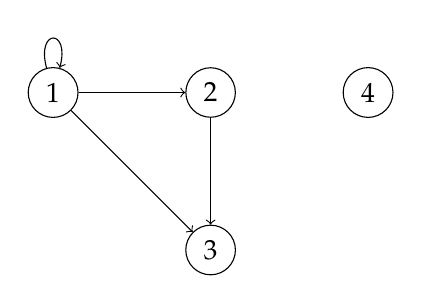
\begin{tikzpicture}[->,node distance=2cm]
  \node[draw,circle] (A) {$1$};
  \node[draw,circle] (B) [right of=A] {$2$};
  \node[draw,circle] (C) [below of=B] {$3$};
  \node[draw,circle] (D) [right of=B] {$4$};
  \draw (A) to [loop above]  (A);
  \draw (A) to  (B);
  \draw (A) to  (C);
  \draw (B) to  (C);
  \end{tikzpicture}
\intertext{Dit is een andere graaf dan $\tuple{V', E}$ met $V' =
  \{1, 2, 3\}$, die er als volgt uitziet:}
& 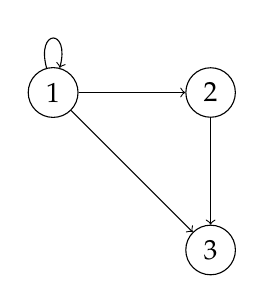
\begin{tikzpicture}[->,node distance=2cm]
  \node[draw,circle] (A) {$1$};
  \node[draw,circle] (B) [right of=A] {$2$};
  \node[draw,circle] (C) [below of=B] {$3$};
  \draw (A) to [loop above]  (A);
  \draw (A) to  (B);
  \draw (A) to  (C);
  \draw (B) to  (C);
  \end{tikzpicture}
\end{align*}
\end{ex}

\begin{prob}
  Beschouw de relatie ‘kleiner dan of gelijk aan’~$\le$ op de
  verzameling $\{1, 2, 3, 4\}$ als een graaf en teken het bijbehorende
  diagram.
\end{prob}
% END ACCEPTED BODY OLP-0017
\endgroup
% END ACCEPTED UNIT OLP-0017

% BEGIN ACCEPTED UNIT OLP-0018 path=translations/nl-standard/content/sets-functions-relations/relations/trees.tex source-sha256=a41f1be466003158eb892735d6acecd66e0e95f446c7ff6488bd665bb76d6825
\begingroup
\def\olfilename{OLP-0018}
\def\olfilepath{content/sets-functions-relations/relations/}
\hypertarget{unit-OLP-0018}{}
\typeout{PARTIAL-READER-UNIT OLP-0018}
% BEGIN ACCEPTED BODY OLP-0018 body-sha256=f0cf709fff998ec8e9e35c950251638153d525bda30d328e4eba98f7ecaf6120
% Part: sets-functions-relations
% Chapter: relations
% Section: trees



\olfileid{sfr}{rel}{tre}
\olsection{Bomen}

Een \emph{boom} is een bijzonder soort partiële ordening die in alle
deelgebieden van de logica een belangrijke rol speelt. Eindige bomen
komen voor in elementaire onderdelen van de logica: zo kunnen
!!{formula}s worden begrepen aan de hand van hun ontleding in een
syntaxisboom, terwijl !!{derivation}s in veel systemen voor
!!{derivation}s eveneens de vorm van eindige bomen hebben.
%
Oneindige bomen komen al voor in bewijzen van de
volledigheidsstellingen voor de propositie- en eerste-ordelogica en
worden in de hele wiskundige logica gebruikt.

Het begrip boom uit de verzamelingenleer hangt nauw samen met het
begrip boom uit de grafentheorie. Hieronder staat een afbeelding van
een (eindige) boom:

\begin{center}
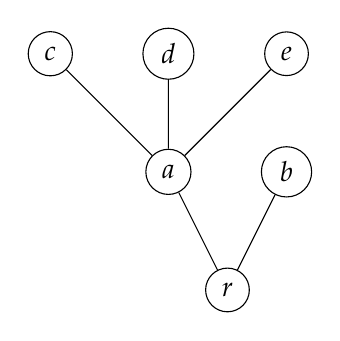
\begin{tikzpicture}[nodes={draw, circle}, -]
\node{$r$} [grow'=up]
    child { node {$a$} 
        child { node {$c$} }
        child { node {$d$} }
        child { node {$e$} }
    }
    child { node {$b$} };
\end{tikzpicture}
\end{center}

De onderste knoop~$r$ is de wortel. Elke knoop behalve $r$ heeft vlak
eronder precies één ouder. Voor knopen~$x$ en~$y$ geldt: als $y$
vanuit~$x$ kan worden bereikt door de lijnen omhoog te volgen, dan
noemen we $x$ een \emph{voorouder} van~$y$.

De voorouderrelatie in een boom is een strikte partiële ordening. Dit
vormt de aanleiding voor de definitie in termen van verzamelingen.
Daarvoor zijn twee begrippen nodig. Een \emph{kleinste element} in een
verzameling~$A$ die partieel is geordend door~$\le$, is !!a{element}
$x \in A$ waarvoor bij alle $y \in A$ geldt dat~$x \le y$. Een
verzameling heet door~$\le$ \emph{welgeordend} als iedere niet-lege
deelverzameling een kleinste element heeft.

\begin{defn}[Boom]
Een \emph{boom} is een paar $T = \tuple{A, \le}$ waarvoor $A$ een
verzameling is en $\le$ een partiële ordening op~$A$ is met precies één
kleinste element $r \in A$ (de \emph{wortel}), en waarvoor voor alle
$x \in A$ de verzameling $\Setabs{y}{y \le x}$ door~$\le$
welgeordend is.
\end{defn}

\begin{defn}[Opvolgers]
Stel dat $T = \tuple{A, \le}$ een boom is.
Als $x,y \in A$, $x < y$, en er geen $z \in A$ bestaat waarvoor
$x < z < y$, dan noemen we $y$ een \emph{opvolger} van~$x$.
\end{defn}

De opvolgers van $x \in A$ heten ook zijn \emph{kinderen}. Als $y$
een opvolger van~$x$ is, noemen we $x$ de \emph{voorganger} of
\emph{ouder} van~$y$.

\begin{prop}
Als $\tuple{A,\le}$ een boom is, heeft elk $x \in A$ behalve de wortel
hoogstens één voorganger.
\end{prop}

\begin{proof}
  Stel dat $y_1 < x$ en $y_2 < x$ en dat $y_1 \neq y_2$. Dan geldt
  $\{y_1, y_2\} \subseteq \Setabs{z}{z<x}$. Omdat
  $\Setabs{z}{z<x}$ door~$\le$ welgeordend is, heeft de deelverzameling
  $\{y_1, y_2\}$ een kleinste element, dat uiteraard $y_1$ of~$y_2$
  moet zijn. Dus $y_1 \le y_2$ of $y_2 \le y_1$. We hebben
  $y_1 \neq y_2$ aangenomen, zodat zelfs $y_1 < y_2$ of $y_2 < y_1$
  geldt. Omdat we ook $y_1 < x$ en $y_2 < x$ hebben aangenomen, geldt
  bovendien $y_1 < y_2 < x$ of $y_2 < y_1 < x$. De elementen $y_1$
  en $y_2$ kunnen dus niet beide voorgangers van~$x$ zijn.
\end{proof}

\begin{defn}
Een boom $T = \tuple{A, \le}$ heet \emph{oneindig} als $A$ een
oneindige verzameling is, en anders \emph{eindig}. Als voor $T$ geldt
dat elke $x \in A$ slechts eindig veel opvolgers heeft, heet $T$ \emph{eindig
vertakkend}.
\end{defn}

\begin{defn}[Takken]
Zij $T = \tuple{A, \le}$ een boom. Een \emph{tak} van~$T$ is een
maximale keten in~$T$, d.w.z. een verzameling $B \subseteq A$ waarvoor
voor alle $x, y \in B$ geldt dat $x \le y$ of $y \le x$, en waarvoor
voor elke $z \in A \setminus B$ een $u \in B$ bestaat zodat noch
$z \le u$ noch $u \le z$ geldt.
%
Met $[T]$ duiden we de verzameling van alle takken van $T$ aan.
\end{defn}

\begin{ex}
Een klassiek voorbeeld van een eindig vertakkende boom is de
\emph{oneindige binaire boom} van eindige rijen van $0$'en en~$1$'en.
Deze wordt soms aangeduid met $\{0,1\}^*$ of~$\Bin^*$ en is geordend
door de uitbreidingsrelatie $\sqsubseteq$ (bijv.
$101 \sqsubseteq 101101$). Omdat iedere binaire rij steeds kan worden
uitgebreid door achteraan een $0$ of een $1$ toe te voegen, bevat deze
boom oneindig veel elementen: elk element~$s$ heeft precies twee
opvolgers, $s0$ en~$s1$. De wortel is de lege rij $\emptyseq$.
\end{ex}

\begin{ex}
Iets algemener is ook de verzameling van eindige rijen van natuurlijke
getallen~$\Nat^*$ met de uitbreidingsrelatie~$\sqsubseteq$ een boom.
Deze is duidelijk niet eindig vertakkend: elke $s \in \Nat^*$ heeft
oneindig veel opvolgers~$sn$, één voor elke $n \in \Nat$. Elke
$A \subseteq \Nat^*$ die onder~$\sqsubseteq$ gesloten is, is een
\emph{deelboom} van~$\Nat^*$. (Dat wil zeggen: $A$ is zo dat uit
$s \in A$ en $s' \sqsubseteq s$ ook $s' \in A$ volgt.) Alle eindige
bomen kunnen worden weergegeven als eindige deelbomen van~$\Nat^*$.
\end{ex}

\begin{prop}[Lemma van K\H{o}nig]
Als $T = \tuple{A,\le}$ een eindig vertakkende oneindige boom is, dan
heeft $T$ een oneindige tak.
\end{prop}

In de berekenbaarheidstheorie gebruikt men vaak een speciaal geval van
het lemma van K\H{o}nig. Dit staat bekend als het \emph{zwakke lemma van
K\H{o}nig}: elke oneindige deelboom van $\{0,1\}^*$ heeft een
oneindige tak.
% END ACCEPTED BODY OLP-0018
\endgroup
% END ACCEPTED UNIT OLP-0018

% BEGIN ACCEPTED UNIT OLP-0019 path=translations/nl-standard/content/sets-functions-relations/relations/operations.tex source-sha256=0c98682bb9d4e3def558b9420af2d21ab653a26df043f6331e9735f1d5c172e1
\begingroup
\def\olfilename{OLP-0019}
\def\olfilepath{content/sets-functions-relations/relations/}
\hypertarget{unit-OLP-0019}{}
\typeout{PARTIAL-READER-UNIT OLP-0019}
% BEGIN ACCEPTED BODY OLP-0019 body-sha256=fee64dd43ac1f1da42c9de9263dfd0ca14131ba3cc63311aac7843c5bcfc77b8
% Part: sets-functions-relations
% Chapter: relations
% Section: operations



\olfileid{sfr}{rel}{ops}
\olsection{Bewerkingen op relaties}

Het is vaak nuttig relaties te wijzigen of te combineren. In
\olref[sfr][rel][ord]{prop:stricttopartial} hebben we de \emph{vereniging}
van relaties beschouwd. Dit is eenvoudig de vereniging van twee relaties die
we opvatten als verzamelingen van paren. Evenzo hebben we in
\olref[sfr][rel][ord]{prop:partialtostrict} het relatieve verschil van relaties
beschouwd. Hieronder volgen enkele andere bewerkingen op relaties.

\begin{defn}\ollabel{relationoperations} 
Laat $R$ en $S$ relaties zijn en $A$ een willekeurige verzameling.

De \emph{inverse} van $R$ is $R^{-1} = \Setabs{\tuple{y, x}}{\tuple{x,
    y} \in R}$.

De \emph{samenstelling} van $R$ en $S$ (eerst de eerste relatie, daarna de
tweede) is $(R \mid S) =
\{\tuple{x, z} : \exists y(Rxy \land Syz)\}$.

De \emph{restrictie} van $R$ tot $A$ is $\funrestrictionto{R}{A}= R
\cap A^2$.

Het door $R$ bepaalde \emph{beeld} van $A$ is $\funimage{R}{A} = \{y :
(\exists x \in A)Rxy\}$.
\end{defn}

\begin{ex}
Laat $S \subseteq \Int^2$ de opvolgerrelatie op~$\Int$ zijn, dus
$S = \Setabs{\tuple{x, y} \in \Int^2}{x + 1 = y}$. Dan geldt $Sxy$ precies
dan wanneer $x + 1 = y$.

$S^{-1}$ is de voorgangerrelatie op $\Int$, dus
$\Setabs{\tuple{x,y}\in\Int^2}{x -1 =y}$.

$S\mid S$ is
$ \Setabs{\tuple{x,y}\in\Int^2}{x + 2 =y}$

$\funrestrictionto{S}{\Nat}$ is de opvolgerrelatie op~$\Nat$.

$\funimage{S}{\{1,2,3\}}$ is $\{2, 3, 4\}$.
\end{ex}

\begin{defn}[Transitieve afsluiting]Laat $R \subseteq A^2$ een binaire relatie zijn.
	
De \emph{transitieve afsluiting} van~$R$ is $R^+ = \bigcup_{0 < n \in
\Nat} R^n$, waarbij we recursief $R^1 = R$ en $R^{n+1} = R^n
\mid R$ definiëren.

De \emph{reflexief-transitieve afsluiting} van $R$ is $R^* = R^+ \cup
\Id{A}$.
\end{defn}

\begin{ex}
Neem de opvolgerrelatie $S \subseteq \Int^2$. Dan geldt $S^2xy$ precies als
$x + 2 = y$, $S^3xy$ precies als $x + 3 = y$, enzovoort. Dus geldt $S^+xy$
precies als $x + n = y$ voor een zekere $n \geq 1$. Anders gezegd: $S^+xy$
geldt precies als $x < y$, en $S^*xy$ precies als $x \le y$.
\end{ex}

\begin{prob}
Toon aan dat de transitieve afsluiting van $R$ inderdaad transitief is.
\end{prob}
% END ACCEPTED BODY OLP-0019
\endgroup
% END ACCEPTED UNIT OLP-0019
\OLEndChapterHook

% BEGIN ACCEPTED UNIT OLP-0020 path=translations/nl-standard/content/sets-functions-relations/functions/functions.tex source-sha256=095199b52971703373d2cd9bfd0103450e30a405145e63084981deba8bef1a60
\begingroup
\def\olfilename{OLP-0020}
\def\olfilepath{content/sets-functions-relations/functions/}
\hypertarget{unit-OLP-0020}{}
\typeout{PARTIAL-READER-UNIT OLP-0020}
% BEGIN ACCEPTED BODY OLP-0020 body-sha256=aac34667a2f86c82d6ddb67aeb2ecfd3f72f23f3edf8551699815f2d9c30070a
% Part: sets-functions-relations
% Chapter: functions



\olchapter{sfr}{fun}{Functies}
% END ACCEPTED BODY OLP-0020
\endgroup
% END ACCEPTED UNIT OLP-0020

% BEGIN ACCEPTED UNIT OLP-0021 path=translations/nl-standard/content/sets-functions-relations/functions/function-basics.tex source-sha256=8c2c0f59873989026d21d20f5aec234049800a2496ba2d9a4f098a91214d12d1
\begingroup
\def\olfilename{OLP-0021}
\def\olfilepath{content/sets-functions-relations/functions/}
\hypertarget{unit-OLP-0021}{}
\typeout{PARTIAL-READER-UNIT OLP-0021}
% BEGIN ACCEPTED BODY OLP-0021 body-sha256=f726152c597b82bd88e631ea904459e61b483cb71a986bf298379f9857559418
% Part: sets-functions-relations
% Chapter: functions
% Section: basics



\olfileid{sfr}{fun}{bas}
\olsection{Basisbegrippen}

\begin{explain}
Een \emph{functie} beeldt elk !!{element} van een gegeven verzameling af op
één bepaald !!{element} van een (eventueel andere) gegeven verzameling. Zo
bepaalt de bewerking optellen met~$1$ een functie:
elk getal~$n$ wordt afgebeeld op precies één getal~$n+1$.
  
Algemener kunnen functies paren, drietallen enzovoort als argument hebben en
een bepaalde uitvoer opleveren. Veel functies kennen we uit de elementaire
rekenkunde. Optelling en vermenigvuldiging zijn bijvoorbeeld functies: ze
hebben twee getallen als invoer en leveren één getal als uitvoer op.

In deze wiskundige, abstracte betekenis is een functie een \emph{zwarte
doos}: alleen de koppeling tussen invoer en uitvoer is van belang, niet de
methode waarmee de uitvoer wordt berekend.
\end{explain}

\begin{defn}[Functie]
Een \emph{functie} $f \colon A \to B$ beeldt elk !!{element} van~$A$ af
op een !!{element} van~$B$.

We noemen $A$ het \emph{domein} van~$f$ en $B$ het \emph{codomein}
van~$f$. De !!{element}en van~$A$ heten de invoeren of \emph{argumenten}
van~$f$. Het !!{element} van~$B$ dat aan een argument~$x$ door~$f$ wordt
gekoppeld, heet de \emph{waarde van~$f$} voor argument~$x$ en wordt
geschreven als~$f(x)$.

Het \emph{beeld} $\ran{f}$ van~$f$ is de deelverzameling van het codomein
die bestaat uit de waarden van~$f$ voor een of meer argumenten; $\ran{f} =
\Setabs{f(x)}{x \in A}$.
\end{defn}

Het diagram in \olref{fig:function} kan helpen om functies te begrijpen. De
ellips links stelt het \emph{domein} van de functie voor en de ellips rechts
haar \emph{codomein}. Een pijl loopt van een \emph{argument} in het domein
naar de bijbehorende \emph{waarde} in het codomein.

\begin{figure}
  \olasset{assets/diagrams/function.tikz}
  \caption{Een functie beeldt elk !!{element} van de ene verzameling af op
    !!a{element} van een andere. Een pijl loopt van een argument in het
    domein naar de bijbehorende waarde in het codomein.}
  \ollabel{fig:function}
\end{figure}

\begin{ex}
Vermenigvuldiging neemt paren natuurlijke getallen als invoer en beeldt ze
af op natuurlijke getallen als uitvoer. Dit is dus een functie van
$\Nat \times \Nat$ (het domein) naar $\Nat$ (het codomein). Het beeld blijkt
ook $\Nat$ te zijn, want elke $n \in \Nat$ is gelijk aan $n \times 1$.
\end{ex}

\begin{ex}
Vermenigvuldiging is een functie, omdat zij elke invoer---elk paar natuurlijke
getallen---aan precies één uitvoer koppelt: $\times \colon \Nat^2 \to
\Nat$. Daarentegen levert de koppeling van een natuurlijk getal~$n$ aan een
reëel getal~$x$ waarvoor $x^2 = n$ geen functie op, want elk positief geheel
getal~$n$ heeft twee vierkantswortels: $\sqrt{n}$ en~$-\sqrt{n}$. We krijgen
wel een functie als we alleen de niet-negatieve vierkantswortel kiezen:
$\sqrt{\phantom{X}} \colon \Nat \to \Real$.
\end{ex}

\begin{ex}
De relatie die elke leerling in een klas aan diens eindcijfer koppelt, is een
functie: geen leerling kan binnen dezelfde klas twee verschillende eindcijfers
krijgen. De relatie die elke leerling in een klas aan diens ouders koppelt, is
geen functie: een leerling kan nul, twee of meer ouders hebben.
\end{ex}

\begin{explain}
We kunnen een functie definiëren door voor elk mogelijk argument nauwkeurig
vast te leggen wat haar waarde is. Dat kan met een formule, met een methode om
de waarde te berekenen of met een lijst van de waarden voor alle argumenten.
Welke definitiewijze we ook kiezen, voor elk argument moeten we precies één
waarde vastleggen.
\end{explain}


\begin{ex}
Definieer $f \colon \Nat \to \Nat$ door $f(x) = x+1$. Deze definitie legt
$f$ vast als een functie met natuurlijke getallen als invoer en als uitvoer.
Bij een natuurlijk getal~$x$ levert $f$ de opvolger~$x+1$.
In dit geval is het codomein $\Nat$ niet het beeld van~$f$, want het
natuurlijke getal~$0$ is van geen enkel natuurlijk getal de opvolger. Het
beeld van~$f$ is de verzameling van alle positieve gehele getallen,
$\Int^{+}$.
\end{ex}

\begin{ex}\ollabel{examplefunext}
Definieer $g \colon \Nat \to \Nat$ door $g(x) = x+2-1$. Hieruit volgt dat
$g$ een functie is met natuurlijke getallen als invoer en als uitvoer. Bij een
natuurlijk getal~$x$ levert $g$ de voorganger van de opvolger van de opvolger
van~$x$, dus $x+1$.
\end{ex}

\begin{explain}
We hebben zojuist twee functies, $f$ en $g$, met verschillende
\emph{definities} bekeken. Toch zijn ze \emph{dezelfde functie}. Voor elk
natuurlijk getal~$n$ geldt immers $f(n) = n+1 = n+2-1 =
g(n)$. Anders gezegd: onze definities van $f$ en~$g$ leggen met verschillende
vergelijkingen dezelfde afbeelding vast. We gebruiken hier dus stilzwijgend
het extensionaliteitsbeginsel voor functies:
\[
  \text{als }\forall x\, f(x) = g(x)\text{, dan }f = g
\]
mits $f$ en~$g$ hetzelfde domein én hetzelfde codomein hebben.
\end{explain}

\begin{ex}
We kunnen functies ook gevalsgewijs definiëren. Zo kunnen we
$h \colon \Nat \to \Nat$ definiëren door
\[
h(x) =
\begin{cases}
  \frac{x}{2} & \text{als $x$ even is} \\
  \frac{x+1}{2} & \text{als $x$ oneven is.}
\end{cases}
\]
Omdat elk natuurlijk getal even of oneven is, is de uitvoer van deze functie
altijd een natuurlijk getal. Bij een gevalsgewijze definitie moet elke
mogelijke invoer in precies één geval vallen. Soms moet worden bewezen dat de
gevallen uitputtend en onderling uitsluitend zijn.
\end{ex}
% END ACCEPTED BODY OLP-0021
\endgroup
% END ACCEPTED UNIT OLP-0021

% BEGIN ACCEPTED UNIT OLP-0022 path=translations/nl-standard/content/sets-functions-relations/functions/function-kinds.tex source-sha256=ac01f1eb03b2e09e7dcb60c0b3e0a6e180ac3eca8379024fce884b8759a90a1d
\begingroup
\def\olfilename{OLP-0022}
\def\olfilepath{content/sets-functions-relations/functions/}
\hypertarget{unit-OLP-0022}{}
\typeout{PARTIAL-READER-UNIT OLP-0022}
% BEGIN ACCEPTED BODY OLP-0022 body-sha256=8c3ca805f2afc0494bdfb028216e549f2dac3742543b2c412f1bba2856a84a0f
% Part: sets-functions-relations
% Chapter: functions
% Section: kinds



\olfileid{sfr}{fun}{kin}
\olsection{Soorten functies}

\begin{explain}
Het is nuttig een indeling te geven van enkele soorten functies die we
het vaakst tegenkomen.

Om te beginnen bekijken we functies met de eigenschap dat ieder
element van het codomein een waarde van de functie is. Zulke functies
heten !!{surjective} en kunnen worden weergegeven zoals in
\olref{fig:surjective}.

\begin{figure}
  \olasset{assets/diagrams/surjective.tikz}
  \caption{!!^a{surjective} functie heeft ieder !!{element} van het
    codomein als waarde.}
  \ollabel{fig:surjective}
\end{figure}
\end{explain}

\begin{defn}[!!^{surjective} functie]
Een functie $f \colon A \rightarrow B$ heet \emph{!!{surjective}} dan
en slechts dan als $B$ ook het bereik van~$f$ is, dat wil zeggen: voor
iedere $y \in B$ bestaat er ten minste één $x \in A$ waarvoor~$f(x) =
y$, of in symbolen:
\[
  (\forall y \in B)(\exists x \in A)f(x) = y.
\]
Zo'n functie noemen we !!a{surjection} van $A$ naar $B$.
\end{defn}

\begin{explain}
Om aan te tonen dat $f$ !!a{surjection} is, moet men laten zien dat
ieder object in het codomein van $f$ de waarde $f(x)$ is voor een
zekere invoer $x$.

Merk op dat iedere functie !!a{surjection} \emph{induceert}. Gegeven
een functie $f \colon A \to B$ definiëren we immers $f' \colon A \to
\ran{f}$ door $f'(x) = f(x)$. Omdat $\ran{f}$ \emph{per definitie}
gelijk is aan $\Setabs{f(x) \in B}{x \in A}$, is deze functie $f'$
gegarandeerd !!a{surjection}.
\end{explain}

\begin{explain}
Iedere functie beeldt elke mogelijke invoer af op precies één uitvoer.
Er zijn echter ook functies die nooit verschillende invoeren op
dezelfde uitvoer afbeelden. Zulke functies heten !!{injective} en
kunnen worden weergegeven zoals in \olref{fig:injective}.
\begin{figure}
  \olasset{assets/diagrams/injective.tikz}
  \caption{!!^a{injective} functie beeldt nooit twee verschillende
    argumenten af op dezelfde waarde.}
  \ollabel{fig:injective}
\end{figure}
\end{explain}

\begin{defn}[!!^{injective} functie]
Een functie $f \colon A \rightarrow B$ heet \emph{!!{injective}} dan
en slechts dan als er voor iedere $y \in B$ ten hoogste één $x \in A$
bestaat waarvoor~$f(x) = y$. Zo'n functie noemen we !!a{injection} van
$A$ naar~$B$.
\end{defn}

\begin{explain}
Om aan te tonen dat $f$ !!a{injection} is, moet men voor willekeurige
!!{element}s $x$ en $y$ van het domein van $f$ bewijzen dat uit
$f(x)=f(y)$ volgt dat $x=y$.
\end{explain}

\begin{ex}
De constante functie $f\colon \Nat \to \Nat$ gegeven door $f(x) = 1$
is noch !!{injective}, noch !!{surjective}.

De identiteitsfunctie $f\colon \Nat \to \Nat$ gegeven door $f(x) = x$
is zowel !!{injective} als !!{surjective}.

De opvolgerfunctie $f \colon \Nat \to \Nat$ gegeven door $f(x) = x+1$
is !!{injective}, maar niet !!{surjective}.
  
De functie $f \colon \Nat \to \Nat$ gedefinieerd door
\[
  f(x) =
  \begin{cases}
    \frac{x}{2} & \text{als $x$ even is} \\
    \frac{x+1}{2} & \text{als $x$ oneven is.}
  \end{cases}
\]
is !!{surjective}, maar niet !!{injective}.
\end{ex}

\begin{explain}
Vaak willen we functies beschouwen die zowel !!{injective} als
!!{surjective} zijn. Zulke functies noemen we !!{bijective}. Ze zien
eruit als de functie in \olref{fig:bijective}. !!^{bijection}s worden
ook wel \emph{een-eenduidige correspondenties} genoemd, omdat ze de
elementen van het codomein eenduidig koppelen aan de elementen van het
domein.
\begin{figure}
  \olasset{assets/diagrams/bijective.tikz}
  \caption{!!^a{bijective} functie koppelt de elementen van het
    codomein eenduidig aan die van het domein.}
  \ollabel{fig:bijective}
\end{figure}
\end{explain}

\begin{defn}[!!^{bijection}]
Een functie $f \colon A \to B$ heet \emph{!!{bijective}} dan en
slechts dan als zij zowel !!{surjective} als !!{injective} is. Zo'n
functie noemen we !!a{bijection} van $A$ naar~$B$ (of tussen $A$
en~$B$).
\end{defn}
% END ACCEPTED BODY OLP-0022
\endgroup
% END ACCEPTED UNIT OLP-0022

% BEGIN ACCEPTED UNIT OLP-0023 path=translations/nl-standard/content/sets-functions-relations/functions/functions-relations.tex source-sha256=5341dcb617e56fcae1fe35d4d1a7dd8087a8be13b1f6a313648f2f1d8df02304
\begingroup
\def\olfilename{OLP-0023}
\def\olfilepath{content/sets-functions-relations/functions/}
\hypertarget{unit-OLP-0023}{}
\typeout{PARTIAL-READER-UNIT OLP-0023}
% BEGIN ACCEPTED BODY OLP-0023 body-sha256=b01e55760f061927d82806449aecbc9b5e251ddf3a7e54a02bf048bd83b6bacf
% Part: sets-functions-relations
% Chapter: functions
% Section: functions-relations




\olfileid{sfr}{fun}{rel}

\olsection{Functies als relaties}

\begin{explain}
Een functie die !!{element}s van~$A$ afbeeldt op !!{element}s van~$B$
bepaalt vanzelf een relatie tussen $A$ en~$B$, namelijk de relatie die
tussen $x$ en $y$ geldt dan en slechts dan als $f(x) = y$. We kunnen
de functie~$f$ zelfs---bijvoorbeeld als we het aantal bouwstenen van
de wiskunde willen beperken---\emph{identificeren} met deze relatie,
dus met een verzameling paren. Dit roept de vraag op: welke relaties
bepalen op deze manier functies?
\end{explain}

\begin{defn}[Grafiek van een functie] Laat $f\colon A \to B$ een
functie zijn. De \emph{grafiek} van~$f$ is de relatie $R_f \subseteq A
\times B$ die wordt gedefinieerd door
\[
R_f = \Setabs{\tuple{x,y}}{f(x) = y}.
\]
\end{defn}

\begin{explain}
Uit extensionaliteit volgt dat de grafiek van een functie uniek is.
Bovendien rechtvaardigt extensionaliteit voor verzamelingen direct het
stilzwijgende extensionaliteitsbeginsel voor functies: als $f$ en~$g$
hetzelfde domein en codomein hebben, zijn ze gelijk wanneer ze overal
dezelfde waarden aannemen.

Evenzo is een ‘functionele’ relatie de grafiek van een functie.
\end{explain}

\begin{prop}\ollabel{prop:graph-function}
Laat $R \subseteq A \times B$ aan de volgende voorwaarden voldoen:
\begin{enumerate}
\item Als $Rxy$ en $Rxz$, dan $y = z$; en
\item voor iedere $x \in A$ bestaat er een $y \in B$ waarvoor
$\tuple{x, y} \in R$.
\end{enumerate}
Dan is $R$ de grafiek van de functie $f\colon A \to B$ die wordt
gedefinieerd door $f(x) = y$ dan en slechts dan als $Rxy$.
\end{prop}

\begin{proof}
Stel dat er een $y$ bestaat waarvoor $Rxy$ geldt. Als er nog een $z
\neq y$ bestond waarvoor $Rxz$ geldt, zou niet aan de voorwaarde
voor~$R$ zijn voldaan. Als er een $y$ bestaat waarvoor $Rxy$ geldt, is
deze $y$ dus uniek en is $f$ goed gedefinieerd. Uiteraard is $R_f =
R$.
\end{proof}

\begin{explain}
Iedere functie $f\colon A \to B$ heeft een grafiek, dat wil zeggen een
relatie die bestaat uit paren in $A \times B$ en wordt gedefinieerd
door $f(x) = y$.
Omgekeerd is iedere relatie~$R \subseteq A \times B$ met de
eigenschappen uit \olref{prop:graph-function} de grafiek van een
functie~$f \colon A \to B$. Door dit nauwe verband tussen functies en
hun grafieken kunnen we een functie eenvoudig als haar grafiek
opvatten. Functies kunnen met andere woorden worden geïdentificeerd
met bepaalde relaties, dus met bepaalde verzamelingen tupels.
\oliflabeldef{sfr:rel:ref:sec}{Merk echter op dat deze ‘identificatie’
dezelfde strekking heeft als in \olref[sfr][rel][ref]{sec}: het is
geen bewering over de metafysica van functies, maar de vaststelling
dat het handig is functies als bepaalde verzamelingen te
\emph{behandelen}. Een voordeel daarvan is het volgende: w}{W}e
kunnen nu op functies soortgelijke bewerkingen uitvoeren als we op
relaties hebben uitgevoerd (zie \olref[sfr][rel][ops]{sec}). In het
bijzonder:
\end{explain}

\begin{defn}\ollabel{defn:funimage}
Laat $f \colon A \to B$ een functie zijn met $C\subseteq A$.

De \emph{restrictie} van~$f$ tot~$C$ is de
functie~$\funrestrictionto{f}{C}\colon C \to B$ die wordt gedefinieerd
door $(\funrestrictionto{f}{C})(x) = f(x)$ voor alle $x \in C$. Met
andere woorden, $\funrestrictionto{f}{C} = \Setabs{\tuple{x, y} \in
R_f}{x \in C}$.

Als we~$f$ op~$C$ \emph{toepassen}, krijgen we $\funimage{f}{C} =
\Setabs{f(x)}{x \in C}$. Dit noemen we ook het \emph{beeld} van~$C$
onder~$f$.
\end{defn}

\begin{explain}
Uit deze definities volgt dat $\ran{f} =
\funimage{f}{\dom{f}}$ voor iedere functie~$f$.
\oliflabeldef{sfr:rel:ops:sec}{Deze begrippen werken precies zoals men
op grond van de definities in \olref[sfr][rel][ops]{sec} en onze
identificatie van functies met relaties zou verwachten. Twee andere
bewerkingen---inversen en samenstellingen van relaties---vereisen echter iets
meer uitleg. Die geven we in \olref[inv]{sec} en
\olref[cmp]{sec}.}{}
\end{explain}
% END ACCEPTED BODY OLP-0023
\endgroup
% END ACCEPTED UNIT OLP-0023

% BEGIN ACCEPTED UNIT OLP-0024 path=translations/nl-standard/content/sets-functions-relations/functions/inverses.tex source-sha256=92fe714a00857dc69f40c4bc946bccd5532a0493fcd8c4c386b301c1d52f6542
\begingroup
\def\olfilename{OLP-0024}
\def\olfilepath{content/sets-functions-relations/functions/}
\hypertarget{unit-OLP-0024}{}
\typeout{PARTIAL-READER-UNIT OLP-0024}
% BEGIN ACCEPTED BODY OLP-0024 body-sha256=3c10f82e88868dd0b6d90a4531f3e6a23b415828e5eac17cf3b3e2e7aa9e36f9
% Part: sets-functions-relations
% Chapter: functions
% Section: inverses



\olfileid{sfr}{fun}{inv}
\olsection{Inverse functies}

\begin{explain}
We vatten functies op als afbeeldingen. Een voor de hand liggende vraag is
dan of zo'n afbeelding kan worden ``omgekeerd.'' De opvolgerfunctie
$f(x) = x + 1$ kan bijvoorbeeld worden omgekeerd, in die zin dat de
functie $g(y) = y - 1$ ``ongedaan maakt'' wat $f$ doet.

We moeten echter voorzichtig zijn. Met deze definitie is~$g$ wel een
functie $\Int \to \Int$, maar geen \emph{functie} $\Nat \to \Nat$,
omdat $g(0) \notin \Nat$. Zelfs in eenvoudige gevallen is dus niet
meteen duidelijk of een functie kan worden omgekeerd; dat kan van het
domein en codomein afhangen.

Met het begrip inverse van een functie kunnen we dit nauwkeurig formuleren.
\end{explain}

\begin{defn}
Een functie $g \colon B \to A$ is een \emph{inverse} van een functie
$f \colon A \to B$ als $f(g(y)) = y$ en $g(f(x)) = x$ voor alle
$x \in A$ en $y \in B$.
\end{defn}

Als $f$ een inverse~$g$ heeft, schrijven we vaak $f^{-1}$ in plaats
van~$g$.

\begin{explain}
We bepalen nu wanneer functies een inverse hebben. Als inverse van
$f\colon A \to B$ ligt de functie $g\colon B \to A$ voor de hand die
``gedefinieerd wordt door''
\[
g(y) = \text{``de'' $x$ waarvoor $f(x) = y$.}
\]
De aanhalingstekens om ``gedefinieerd wordt door'' (en om ``de'')
geven aan dat dit nog geen geldige definitie is: zo werkt het niet in
alle gevallen. Wil deze definitie een functie
vastleggen, dan moet er precies één~$x$ zijn waarvoor $f(x) = y$:
de uitvoer van~$g$ moet eenduidig zijn bepaald. Bovendien moet die
voor elke $y \in B$ zijn bepaald. Als er $x_1$ en $x_2 \in A$ zijn
waarvoor $x_1 \neq x_2$ maar $f(x_1) = f(x_2)$, dan is $g(y)$ niet
eenduidig bepaald voor $y = f(x_1) = f(x_2)$. En als er helemaal
geen~$x$ bestaat waarvoor $f(x) = y$, dan is $g(y)$ helemaal
niet bepaald. Kortom, om $g$ te kunnen definiëren, moet $f$ zowel
!!{injective} als !!{surjective} zijn.

We werken dit stap voor stap uit en splitsen de vraag in tweeën.
Gegeven een functie~$f\colon A \to B$: wanneer bestaat er een functie
$g\colon B \to A$ waarvoor $g(f(x)) = x$? Zo'n $g$ ``maakt ongedaan''
wat $f$ doet en heet een \emph{linksinverse} van~$f$. Ten tweede:
wanneer bestaat er een functie $h\colon B \to A$ waarvoor
$f(h(y)) = y$? Zo'n $h$ heet een \emph{rechtsinverse} van~$f$:
$f$ ``maakt ongedaan'' wat $h$~doet.
\end{explain}

\begin{prop}
Als het domein niet leeg is en $f\colon A \to B$ !!{injective} is, dan
bestaat er een
\emph{linksinverse}~$g\colon B \to A$ van~$f$ waarvoor
$g(f(x)) = x$ voor alle $x \in A$.
\end{prop}

\begin{proof}
Neem aan dat het domein niet leeg is en dat $f\colon A \to B$
!!{injective} is, en neem $y \in B$.
Als $y \in \ran{f}$, bestaat er een $x \in A$ waarvoor $f(x) = y$.
Omdat $f$ !!{injective} is, bestaat er maar één zo'n~$x \in A$. We
kunnen dan $g(y) = x$ definiëren; $g(y)$ is dus ``de'' $x \in A$
waarvoor $f(x) = y$. Als $y \notin \ran{f}$, kunnen we dit op een
willekeurige~$a \in A$ afbeelden. Kies daarom een $a \in A$ en
definieer $g\colon B \to A$ door:
\[
g(y) = \begin{cases}
    x & \text{als $f(x) = y$}\\
    a & \text{als $y \notin \ran{f}$.}
\end{cases}
\]
Deze functie is voor alle $y \in B$ gedefinieerd, want voor elke
$y \in \ran{f}$ bestaat er precies één $x \in A$ waarvoor $f(x) = y$.
Volgens de definitie geldt: als $y = f(x)$, dan $g(y) = x$, oftewel
$g(f(x)) = x$.
\end{proof}

\begin{prob}
Toon aan dat als $f\colon A \to B$ een linksinverse~$g$ heeft,
$f$~!!{injective} is.
\end{prob}

\begin{prop}
    Als $f\colon A \to B$ !!{surjective} is, dan bestaat er een
    \emph{rechtsinverse}~$h\colon B \to A$ van~$f$ waarvoor
    $f(h(y)) = y$ voor alle~$y \in B$.
\end{prop}

\begin{proof}
Neem aan dat $f\colon A \to B$ !!{surjective} is en neem $y \in B$.
Omdat $f$~!!{surjective} is, bestaat er een $x_y \in A$ waarvoor
$f(x_y) = y$. We kunnen dan $h(y) = x_y$ definiëren. Voor elke
$y \in B$ kiezen we dus een $x \in A$ waarvoor $f(x) = y$; omdat
$f$~!!{surjective} is, valt er altijd ten minste één te
kiezen.\footnote{Omdat $f$ !!{surjective} is, is voor elke~$y \in B$
de verzameling $\Setabs{x}{f(x) = y}$ niet-leeg. Voor onze definitie
van~$h$ moeten we uit elk van deze verzamelingen één $x$ kiezen. Dat
dit altijd mogelijk is, spreekt in feite niet vanzelf: de mogelijkheid
om deze keuzes te maken wordt eenvoudigweg als axioma aangenomen. Met
andere woorden, deze stelling veronderstelt het zogeheten
keuzeaxioma, een kwestie die we
\oliflabeldef{sth:choice::chap}{opnieuw behandelen in \olref[sth][choice][]{chap}}{hier buiten beschouwing laten}.
In veel specifieke gevallen is het keuzeaxioma echter niet nodig,
bijvoorbeeld wanneer $A = \Nat$ of eindig is, of wanneer $f$
!!{bijective} is. (In het bijzondere geval dat $f$ !!{bijective} is,
heeft voor elke $y \in B$ de verzameling $\Setabs{x}{f(x) = y}$
precies één !!{element}, zodat er niets te kiezen valt.)}
Volgens de definitie geldt: als $x = h(y)$, dan $f(x) = y$, oftewel
voor elke $y \in B$: $f(h(y)) = y$.
\end{proof}

\begin{prob}
Toon aan dat als $f\colon A \to B$ een rechtsinverse~$h$ heeft,
$f$~!!{surjective} is.
\end{prob}

\begin{explain}
  Door de ideeën uit het vorige bewijs te combineren, volgt nu dat
  elke !!{bijection} een inverse heeft: er is één functie die zowel
  linksinverse als rechtsinverse van~$f$ is.
\end{explain}

\begin{prop}\ollabel{prop:bijection-inverse}
Als $f\colon A \to B$ !!{bijective} is, bestaat er een
functie~$f^{-1}\colon B \to A$ zodanig dat voor alle $x \in A$
$f^{-1}(f(x)) = x$ en voor alle $y \in B$ $f(f^{-1}(y)) = y$.
\end{prop}

\begin{proof}
Opgave.
\end{proof}

\begin{prob}
Bewijs \olref[sfr][fun][inv]{prop:bijection-inverse}. Definieer
$f^{-1}$, toon aan dat dit een functie is en toon aan dat het een
inverse van~$f$ is, dus dat $f^{-1}(f(x)) = x$ en
$f(f^{-1}(y)) = y$ voor alle $x \in A$ en $y \in B$.
\end{prob}

\begin{explain}
We kunnen inversen op een iets algemenere manier verkrijgen. We zagen
in \olref[kin]{sec} dat elke functie $f$ een !!a{surjection}
$f' \colon A \to \ran{f}$ induceert door $f'(x) = f(x)$ te stellen
voor alle $x \in A$. Als $f$~!!{injective} is, is $f'$ duidelijk
!!{bijective} en heeft deze volgens
\olref{prop:bijection-inverse} dus een unieke inverse. Met een klein
misbruik van notatie noemen we de inverse van $f'$ soms kortweg
``de inverse van~$f$.''
\end{explain}

\begin{prop}\ollabel{prop:left-right}%
  Toon aan dat als $f\colon A \to B$ een linksinverse~$g$ en een
  rechtsinverse~$h$ heeft, $h = g$.
\end{prop}

\begin{proof}
  Opgave.
\end{proof}

\begin{prob}
  Bewijs \olref[sfr][fun][inv]{prop:left-right}.
\end{prob}

\begin{prop}\ollabel{prop:inverse-unique}
Elke functie~$f$ heeft ten hoogste één inverse.
\end{prop}

\begin{proof}
  Neem aan dat $g$ en $h$ beide inversen van~$f$ zijn. Dan is $g$ in
  het bijzonder een linksinverse van~$f$ en $h$ een rechtsinverse.
  Volgens \olref{prop:left-right} geldt $g = h$.
\end{proof}
% END ACCEPTED BODY OLP-0024
\endgroup
% END ACCEPTED UNIT OLP-0024

% BEGIN ACCEPTED UNIT OLP-0025 path=translations/nl-standard/content/sets-functions-relations/functions/composition.tex source-sha256=ee5f8167612c117a4fd509dbbd1814c9c9d0ab08042442e3fe6d55ecd11a8a05
\begingroup
\def\olfilename{OLP-0025}
\def\olfilepath{content/sets-functions-relations/functions/}
\hypertarget{unit-OLP-0025}{}
\typeout{PARTIAL-READER-UNIT OLP-0025}
% BEGIN ACCEPTED BODY OLP-0025 body-sha256=9f573567a787d0477be03130632c6081f8e2e222663ea80e6f36c349ce77ac05
% Part: sets-functions-relations
% Chapter: functions
% Section: composition



\olfileid{sfr}{fun}{cmp}
\olsection{Samenstelling van functies}

\begin{explain}
\oliflabeldef{sfr:fun:inv:sec}{In \olref[inv]{sec} zagen we dat de
inverse~$f^{-1}$ van !!a{bijection}~$f$ zelf een functie is. Een andere
bewerking op functies is samenstelling: w}{W}e kunnen een nieuwe
functie definiëren door twee functies, $f$ en~$g$, samen te stellen:
we passen eerst $f$ toe en daarna~$g$. Dit kan alleen als hun beelden
en domeinen op elkaar aansluiten: het beeld van~$f$ moet een
deelverzameling zijn van het domein van~$g$.
\oliflabeldef{sfr:rel:ops:sec}{Deze bewerking met functies is vergelijkbaar
met de samenstelling van relaties uit
\olref[rel][ops]{sec}.}{}

Een diagram kan het idee van samenstelling verduidelijken. In
\olref{fig:composition} tonen we twee functies $f \colon A \to B$ en
$g \colon B \to C$, met hun samenstelling~$(\comp{f}{g})$. De functie
$(\comp{f}{g}) \colon A \to C$ koppelt elk !!{element} van~$A$ aan
!!a{element} van~$C$. Welk !!{element} van~$C$ bij !!a{element} van
$A$ hoort, leggen we als volgt vast. Gegeven een invoer $x \in A$
passen we eerst de functie $f$ toe op~$x$; dit levert $f(x) = y \in B$
op. Vervolgens passen we de functie $g$ toe op~$y$; dit levert
$g(f(x)) = g(y) = z \in C$ op.
\begin{figure}
  \olasset[2\olphotowidth]{assets/diagrams/composition.tikz}
  \caption{De samenstelling $g \circ f$ van twee functies $f$ en~$g$.}
  \ollabel{fig:composition}
\end{figure}
\end{explain}

\begin{defn}[Samenstelling]
Zij $f\colon A \to B$ en $g\colon B \to C$ functies. De
\emph{samenstelling} van $f$ met~$g$ is $\comp{f}{g} \colon A \to C$,
waarbij $(\comp{f}{g})(x) = g(f(x))$.
\end{defn}

\begin{ex}
Beschouw de functies $f(x) = x + 1$ en $g(x) = 2x$. Omdat
$(\comp{f}{g})(x) = g(f(x))$, nemen we voor elke invoer~$x$ eerst de
opvolger en vermenigvuldigen we het resultaat vervolgens met twee. Hun
samenstelling wordt dus gegeven door $(\comp{f}{g})(x) = 2(x+1)$.
\end{ex}

\begin{prob}
Toon aan dat als $f \colon A \to B$ en $g \colon B \to C$ beide
!!{injective} zijn, ook $\comp{f}{g}\colon A \to C$ !!{injective} is.
\end{prob}

\begin{prob}
Toon aan dat als $f \colon A \to B$ en $g \colon B \to C$ beide
!!{surjective} zijn, ook $\comp{f}{g}\colon A \to C$ !!{surjective}
is.
\end{prob}

\begin{prob}
Stel dat $f \colon A \to B$ en $g \colon B \to C$. Toon aan dat de
grafiek van $\comp{f}{g}$ gelijk is aan $R_f \mid R_g$.
\end{prob}
% END ACCEPTED BODY OLP-0025
\endgroup
% END ACCEPTED UNIT OLP-0025

% BEGIN ACCEPTED UNIT OLP-0026 path=translations/nl-standard/content/sets-functions-relations/functions/partial-functions.tex source-sha256=63424e8812c83602f038e39f4482c2bcc9510b39811cd46b05848e1174209851
\begingroup
\def\olfilename{OLP-0026}
\def\olfilepath{content/sets-functions-relations/functions/}
\hypertarget{unit-OLP-0026}{}
\typeout{PARTIAL-READER-UNIT OLP-0026}
% BEGIN ACCEPTED BODY OLP-0026 body-sha256=cd6e1c30603ac4ee022ba512f01967a0895b4e25afd7d5acff59f0c1710b0e5a
% Part: sets-functions-relations
% Chapter: functions
% Section: partial-functions




\olfileid{sfr}{fun}{par}

\olsection{Partiële functies}

\begin{explain}
Soms is het nuttig de definitie van een functie te versoepelen, zodat
de functiewaarde niet voor elke mogelijke invoer gedefinieerd hoeft te
zijn. Zulke afbeeldingen heten \emph{partiële functies}.
\end{explain}

\begin{defn}
Een \emph{partiële functie} $f \colon A \pto B$ is een afbeelding die
aan elk !!{element} van~$A$ ten hoogste één !!{element} van~$B$
toekent. Als $f$ een element van~$B$ aan $x \in A$ toekent, noemen
we $f(x)$ \emph{gedefinieerd}; anders noemen we dit
\emph{ongedefinieerd}. Als $f(x)$ gedefinieerd is, schrijven we $f(x)
\fdefined$; anders schrijven we $f(x) \fundefined$. Het
\emph{domein} van een partiële functie~$f$ is de deelverzameling
van~$A$ waarop ze gedefinieerd is, dus $\dom{f} = \Setabs{x \in
A}{f(x) \fdefined}$.
\end{defn}

\begin{ex}
Elke functie $f\colon A \to B$ is ook een partiële functie. Partiële
functies die overal op~$A$ gedefinieerd zijn---dus wat we tot nu toe
kortweg een functie noemden---heten ook \emph{totale} functies.
\end{ex}

\begin{ex}
De partiële functie $f \colon \Real \pto \Real$ gegeven door $f(x) =
1/x$ is ongedefinieerd voor $x = 0$ en overal elders gedefinieerd.
\end{ex}

\begin{prob}
Gegeven $f\colon A \pto B$, definieer de partiële functie $g\colon B
\pto A$ als volgt. Voor elke $y \in B$: als er precies één $x \in A$
is waarvoor $f(x) = y$, stel dan $g(y) = x$; schrijf anders $g(y)
\fundefined$. Toon aan dat als $f$ injectief is, $g(f(x)) = x$ voor
alle $x \in \dom{f}$ en $f(g(y)) = y$ voor alle $y \in \ran{f}$.
\end{prob}

\begin{defn}[Grafiek van een partiële functie]
Zij $f\colon A \pto B$ een partiële functie. De \emph{grafiek} van~$f$
is de relatie $R_f \subseteq A \times B$ die wordt gedefinieerd door
\[
R_f = \Setabs{\tuple{x,y}}{f(x) = y}.
\]
\end{defn}

\begin{prop}
Stel dat $R \subseteq A \times B$ de eigenschap heeft dat uit $Rxy$ en
$Rxy'$ volgt dat $y = y'$. Dan is $R$ de grafiek van de partiële
functie $f\colon A \pto B$ die als volgt wordt gedefinieerd: als er een
$y$ is waarvoor $Rxy$, stel dan $f(x) = y$; schrijf anders $f(x)
\fundefined$. Als $R$ bovendien \emph{serieel} is, dat wil zeggen dat
er voor elke $x \in A$ een $y \in B$ bestaat waarvoor $Rxy$, dan is
$f$ totaal.
\end{prop}

\begin{proof}
Stel dat er een $y$ is waarvoor $Rxy$. Als er nog een $y' \neq y$ was
waarvoor $Rxy'$, zou de voorwaarde voor $R$ worden geschonden. Als er
een $y$ is waarvoor $Rxy$, is die $y$ dus uniek en is $f$
welgedefinieerd. Verder geldt onmiddellijk $R_f = R$, en $f$ is totaal
als~$R$ serieel is.
\end{proof}
% END ACCEPTED BODY OLP-0026
\endgroup
% END ACCEPTED UNIT OLP-0026
\OLEndChapterHook

% BEGIN ACCEPTED UNIT OLP-0027 path=translations/nl-standard/content/sets-functions-relations/size-of-sets/size-of-sets-complete.tex source-sha256=a65fa2fbacd794210b47e29ac3a2d89a4f1bd8539d90cce61cd0b76fe423f114
\begingroup
\def\olfilename{OLP-0027}
\def\olfilepath{content/sets-functions-relations/size-of-sets/}
\hypertarget{unit-OLP-0027}{}
\typeout{PARTIAL-READER-UNIT OLP-0027}
% BEGIN ACCEPTED BODY OLP-0027 body-sha256=cb8a3af3d6226f877dea938daca6cf674baf145c29bbfce003e88a207fb9ead2
% Part: sets-functions-relations
% Chapter: size-of-sets-complete



\olchapter{sfr}{siz}{De grootte van verzamelingen}

\begin{editorial}
Dit hoofdstuk behandelt opsommingen, aftelbaarheid en
overaftelbaarheid. Verscheidene paragrafen bestaan in twee versies: een
meer elementaire versie die opsommingen opvat als lijsten of als
surjecties vanuit $\PosInt$, en een abstractere versie die opsommingen
definieert als bijecties met $\Nat$.
\end{editorial}











\begin{editorial}
De volgende paragrafen, \olref[sfr][siz][enm-alt]{sec},
\olref[sfr][siz][nen-alt]{sec} en \olref[sfr][siz][red-alt]{sec}, zijn
alternatieve versies van \olref[sfr][siz][enm]{sec},
\olref[sfr][siz][nen]{sec} en \olref[sfr][siz][red]{sec}. Tim Button
schreef ze voor zijn tekst Open Set Theory. Ze zijn iets gevorderder
en gebruiken een andere definitie van opsombaarheid die beter past in
de verzamelingenleer: een bijectie met $\Nat$ of met een beginsegment,
in plaats van de eis dat iets in een lijst kan worden gezet of het
beeld is van een surjectieve functie vanuit $\PosInt$.
\end{editorial}
% END ACCEPTED BODY OLP-0027
\endgroup
% END ACCEPTED UNIT OLP-0027

% BEGIN ACCEPTED UNIT OLP-0028 path=translations/nl-standard/content/sets-functions-relations/size-of-sets/introduction.tex source-sha256=2ec30bea8439de46c54a832541e4a5487f24ec6f673473f70a9380e34a69016b
\begingroup
\def\olfilename{OLP-0028}
\def\olfilepath{content/sets-functions-relations/size-of-sets/}
\hypertarget{unit-OLP-0028}{}
\typeout{PARTIAL-READER-UNIT OLP-0028}
% BEGIN ACCEPTED BODY OLP-0028 body-sha256=c3f9252d0e1a5ba71a732a1b0b02ec265dfb264c3e41c6ed515921639c383c0f
% Part:sets-functions-relations
% Chapter: size-of-sets
% Section: introduction



\olfileid{sfr}{siz}{int}

\olsection{Inleiding}

Toen Georg Cantor in de jaren 1870 de verzamelingenleer ontwikkelde, wilde hij
onder meer het idee van een oneindige verzameling aanvaardbaar maken---een
actuele oneindigheid, zoals de middeleeuwers zouden zeggen. Een belangrijk
onderdeel daarvan was zijn behandeling van de \emph{grootte} van verschillende
verzamelingen. Als $a$, $b$ en $c$ alle verschillend zijn, is de verzameling
$\{a, b, c\}$ intuïtief \emph{groter} dan $\{a, b\}$. Maar hoe zit dat bij
oneindige verzamelingen? Zijn die allemaal even groot? Dat blijkt niet zo te
zijn.

Het eerste belangrijke begrip is dat van een opsomming. Iedere eindige
verzameling kan worden opgesomd door al haar !!{element}s in een lijst te
zetten. Ook van sommige oneindige verzamelingen kunnen we alle !!{element}s
opsommen, mits de lijst zelf oneindig mag zijn. Zulke verzamelingen heten
!!{enumerable}. Cantors verrassende resultaat, dat we aan het einde van dit
hoofdstuk volledig zullen begrijpen, luidt dat sommige oneindige verzamelingen
niet !!{enumerable} zijn.
% END ACCEPTED BODY OLP-0028
\endgroup
% END ACCEPTED UNIT OLP-0028

% BEGIN ACCEPTED UNIT OLP-0029 path=translations/nl-standard/content/sets-functions-relations/size-of-sets/enumerability.tex source-sha256=86067379c2cfea6ca3a8e4c1ae0d8bf2e62186ab7ae42801ea052fc33ed61715
\begingroup
\def\olfilename{OLP-0029}
\def\olfilepath{content/sets-functions-relations/size-of-sets/}
\hypertarget{unit-OLP-0029}{}
\typeout{PARTIAL-READER-UNIT OLP-0029}
% BEGIN ACCEPTED BODY OLP-0029 body-sha256=fc9126ec040bd02efce10690148bccd657ccb40431a58b36fa606a376261d616
% Part:sets-functions-relations
% Chapter: size-of-sets
% Section: enumerations



\olfileid{sfr}{siz}{enm}

\olsection{Opsommingen en \usetoken{S}{enumerable} verzamelingen}

\begin{editorial}
  Deze paragraaf bespreekt opsommingen van verzamelingen en definieert
  ze als surjectieve functies met $\PosInt$ als domein. De uitleg gaat stap voor stap,
  voor lezers met weinig wiskundige achtergrond. In
  \olref[enm-alt]{sec} staat een alternatieve, beknoptere versie, die
  opsommingen anders definieert: als bijecties tussen $\Nat$ (of een
  beginsegment daarvan) en de opgesomde verzameling.
\end{editorial}

\begin{explain}
We hebben al voorbeelden van verzamelingen gegeven door hun
!!{element}s op te sommen. We bespreken nu algemener hoe en wanneer
we de !!{element}s van een verzameling kunnen opsommen, ook als die
verzameling oneindig is.
\end{explain}

\begin{defn}[Opsomming, informeel]
Informeel is een \emph{opsomming} van een verzameling~$A$ een mogelijk
oneindige lijst van !!{element}s van~$A$ waarin ieder !!{element} van $A$
op een eindige plaats voorkomt. Als $A$ een opsomming heeft, heet $A$
\emph{!!{enumerable}}.
\end{defn}

\begin{explain}
Enkele opmerkingen over opsommingen:
\begin{enumerate}
\item We rekenen alleen lijsten met een begin tot de opsommingen. Ook
  moet ieder !!{element} behalve het eerste precies één !!{element}
  direct vóór zich hebben. Met andere woorden: tussen het eerste
  !!{element} van de lijst en elk ander !!{element} liggen slechts
  eindig veel elementen. Ieder !!{element} van een opsomming heeft dus
  een eindige plaats: het eerste !!{element} heeft plaats~$1$, het
  tweede plaats~$2$, enzovoort.
\item Dezelfde verzameling~$A$ kan verschillende opsommingen hebben
  waarin de !!{element}s in een andere volgorde staan: $4$, $1$,
  $25$, $16$,~$9$ somt de verzameling van de eerste vijf kwadraten
  even goed op als $1$, $4$, $9$, $16$,~$25$.
\item Een opsomming met herhalingen blijft een opsomming: $1$, $1$, $2$,
  $2$, $3$, $3$,~\dots{} somt dezelfde verzameling op als $1$, $2$,
  $3$,~\dots{}.
\item Volgorde en herhaling zijn \emph{wel} van belang wanneer we een
  opsomming vastleggen: we kunnen een opsomming van de positieve gehele
  getallen laten beginnen met $1$, $2$, $3$, $1$, \dots{}, maar het patroon is duidelijker in
  de gebruikelijke opsomming $1$, $2$, $3$, $4$,~\dots
\item Een opsomming moet een begin hebben: \dots, $3$, $2$, $1$ is geen
  opsomming van de positieve gehele getallen, want zij heeft geen eerste
  !!{element}. Dit volgt uit de informele definitie: vraag bijvoorbeeld
  op welke plaats in de lijst het getal 76 voorkomt.
\item De volgende lijst is geen opsomming van de positieve gehele getallen:
  $1$, $3$, $5$, \dots, $2$, $4$, $6$, \dots\@ Het probleem is dat de
  even getallen op de plaatsen $\infty + 1$, $\infty + 2$, $\infty +
  3$ staan, en niet op eindige plaatsen.
\item De lege verzameling is aftelbaar: de lege lijst somt haar op!{}
\end{enumerate}
\end{explain}

\begin{prop}
  Als $A$ een opsomming heeft, heeft zij ook een opsomming zonder
  herhalingen.
\end{prop}

\begin{proof}
  Stel dat $A$ een opsomming $x_1$, $x_2$, \dots{} heeft waarin elke
  $x_i$ een !!{element} van~$A$ is. We kunnen herhalingen verwijderen
  door herhaalde !!{element}s weg te laten. Zo verkrijgen we een nieuwe
  opsomming: we nemen $x_i$ op als dit !!a{element} van~$A$ nog niet
  voorkomt onder $x_1$, \dots, $x_{i-1}$. We laten $x_i$ uit de lijst
  weg als het al voorkomt onder $x_1$, \dots,~$x_{i-1}$.
\end{proof}

Het vorige argument laat zien dat we een nauwkeurigere definitie nodig
hebben om opsommingen en !!{enumerable} verzamelingen goed te begrijpen
en er uitspraken over te bewijzen. Die definitie volgt nu.

\begin{defn}[Opsomming, formeel] 
Een \emph{opsomming} van een verzameling $A \neq \emptyset$ is iedere
!!{surjective} functie $f \colon \PosInt \to A$.
\end{defn}

\begin{explain}
We gaan na dat de formele definitie gelijkwaardig is aan de informele
definitie met een mogelijk oneindige lijst. Om te beginnen somt iedere
!!{surjective} functie van $\PosInt$ naar een verzameling~$A$ de
verzameling~$A$ op. Zo'n functie bepaalt een opsomming in de informele
betekenis hierboven: de lijst $f(1)$, $f(2)$, $f(3)$, \dots. Omdat $f$
!!{surjective} is, is ieder !!{element} van~$A$ de waarde van~$f(n)$
voor een zekere~$n \in \PosInt$. Ieder !!{element} van $A$ komt dus op
een eindige plaats in de lijst voor. Omdat de functie niet
!!{injective} hoeft te zijn, mag de lijst herhalingen bevatten; dat is
zoals gezegd toegestaan.

Omgekeerd kunnen we uit een lijst die alle !!{element}s van~$A$ opsomt
een !!a{surjective} functie $f\colon \PosInt \to A$ definiëren: $f(n)$
is het $n$-de !!{element} van de lijst, of het laatste !!{element} van
de lijst als er geen $n$-de !!{element} is. Alleen wanneer $A$ leeg is,
en de lijst dus leeg is, levert dit geen !!a{surjective} functie op.
Iedere niet-lege lijst bepaalt daarom een !!a{surjective} functie
$f\colon \PosInt \to A$.
\end{explain}

\begin{defn}
  \ollabel{defn:enumerable}
  Een verzameling~$A$ is !!{enumerable} precies dan als zij leeg is of
  een opsomming heeft.
\end{defn}

\begin{ex}
Een functie die de positieve gehele getallen ($\PosInt$) opsomt, is
eenvoudigweg de identiteitsfunctie gegeven door $f(n) = n$. De functie
die de natuurlijke getallen $\Nat$ opsomt, is $g(n) = n - 1$.
\end{ex}

\begin{ex}
De functies $f\colon \PosInt \to \PosInt$ en $g \colon \PosInt \to
\PosInt$, gegeven door
\begin{align*}
f(n) & = 2n \text{ en}\\
g(n) & = 2n - 1
\end{align*}
sommen respectievelijk de positieve even en de positieve oneven gehele
getallen op. Geen van beide functies is echter een opsomming van
$\PosInt$, want geen van beide is !!{surjective}.
\end{ex}

\begin{prob}
Definieer een opsomming van de positieve kwadraten $1$, $4$, $9$, $16$, \dots
\end{prob}

\begin{ex}
De functie $f(n) = (-1)^{n} \lceil \frac{(n-1)}{2}\rceil$ (waarbij
$\lceil x \rceil$ de \emph{plafondfunctie} voorstelt, die het kleinste
gehele getal groter dan of gelijk aan $x$ oplevert) somt de verzameling
gehele getallen~$\Int$ op. Merk op hoe $f$ de getallen uit $\Int$
opsomt door heen en weer te ``springen'' tussen positieve en
negatieve gehele getallen:
\[
\begin{array}{c c c c c c c c}
f(1) & f(2) & f(3) & f(4) & f(5) & f(6) & f(7) & \dots \\ \\
- \lceil \tfrac{0}{2} \rceil & \lceil \tfrac{1}{2}\rceil & - \lceil \tfrac{2}{2} \rceil & \lceil \tfrac{3}{2} \rceil & - \lceil \tfrac{4}{2} \rceil  & \lceil \tfrac{5}{2}
\rceil & - \lceil \tfrac{6}{2} \rceil & \dots \\ \\
0 & 1 & -1 & 2 & -2 & 3 & \dots
\end{array}
\]
We kunnen $f$ ook als volgt per geval definiëren:
\[
f(n) = \begin{cases}
  0 & \text{als $n = 1$}\\
  n/2 & \text{als $n$ even is}\\
  -(n-1)/2 & \text{als $n$ oneven en $>1$ is}
  \end{cases}
\]
\end{ex}

\begin{prob}
  Toon aan dat als $A$ en $B$ !!{enumerable} zijn, ook $A \cup B$ dat is.
  Neem daartoe aan dat er !!{surjective} functies $f\colon \PosInt \to
  A$ en $g\colon \PosInt \to B$ bestaan. Definieer een !!a{surjective}
  functie~$h\colon \PosInt \to A \cup B$ en bewijs dat deze
  !!{surjective} is. Beschouw ook de gevallen waarin $A$ leeg is
  of~$B = \emptyset$.
\end{prob}
  
\begin{prob}
  Toon aan dat als $B \subseteq A$ en $A$ !!{enumerable} is, ook~$B$
  dat is. Neem daartoe aan dat er een !!a{surjective} functie
  $f\colon \PosInt \to A$ bestaat. Definieer een !!a{surjective} functie
  $g\colon \PosInt \to B$ en bewijs dat deze !!{surjective} is. Wat
  gebeurt er als $B = \emptyset$?
\end{prob}
    
\begin{prob}
  Toon met inductie naar $n$ aan dat als $A_1$, $A_2$, \dots, $A_n$
  allemaal !!{enumerable} zijn, ook $A_1 \cup \dots \cup A_n$ dat is.
  Je mag gebruiken dat als twee verzamelingen $A$ en~$B$ !!{enumerable}
  zijn, ook~$A \cup B$ dat is. 
\end{prob}

Hoewel het bij het opsommen van de !!{element}s van een verzameling
wellicht natuurlijker is om vanaf het $1$-ste !!{element} te tellen,
gebruiken wiskundigen daarvoor graag de natuurlijke getallen~$\Nat$.
De !!{element}s van een lijst heten dan achtereenvolgens het $0$-de,
$1$-ste, $2$-de, enzovoort. Daarom kunnen we een
opsomming ook definiëren als een !!a{surjective} functie van $\Nat$
naar~$A$. De twee definities zijn uiteraard gelijkwaardig.

\begin{prop}\ollabel{prop:enum-shift}
  Er bestaat een !!a{surjection} $f\colon \PosInt \to A$ precies dan
  als er een !!a{surjection} $g\colon \Nat \to A$ bestaat.
\end{prop}

\begin{proof}
  Gegeven een !!a{surjection} $f\colon \PosInt \to A$ definiëren we
  $g(n) = f(n+1)$ voor alle $n \in \Nat$. Men ziet direct dat
  $g\colon \Nat \to A$ !!{surjective} is. Omgekeerd definiëren we bij
  een !!a{surjection} $g\colon \Nat \to A$ de functie
  $f(n) = g(n-1)$.
\end{proof}

Hieruit volgt:

\begin{cor}\ollabel{cor:enum-nat}
Een verzameling $A$ is !!{enumerable} precies dan als zij leeg is of er
een !!a{surjective} functie $f\colon \Nat \to A$ bestaat.
\end{cor}

Hierboven hebben we besproken dat een lijst van !!{element}s van een
verzameling~$A$ kan worden omgezet in een lijst zonder herhalingen. Dat
geldt ook voor opsommingen, maar is iets moeilijker nauwkeurig te
formuleren en te bewijzen. Iedere functie $f\colon \PosInt \to A$ moet
voor alle $n \in \PosInt$ gedefinieerd zijn. Als~$A$ maar eindig veel
!!{element}s heeft, kan een functie op de oneindig vele !!{element}s
van~$\PosInt$ niet alle !!{element}s van~$A$ als waarden aannemen zonder
ooit een waarde te herhalen. Wanneer de lijst zonder herhalingen eindig
is, moeten we daarom voor~$f$ een ander domein kiezen, met slechts eindig
veel !!{element}s. Geen herhalingen hebben betekent dat $f$
!!{injective} moet zijn. Omdat de functie ook !!{surjective} is, zoeken
we een !!a{bijection} tussen een eindige verzameling $\{1, \dots, n\}$
of $\PosInt$ en~$A$.

\begin{prop}\ollabel{prop:enum-bij}
Als $f\colon \PosInt \to A$ !!{surjective} is (dus een opsomming
van~$A$), bestaat er een !!a{bijection} $g\colon Z \to A$, waarbij $Z$
gelijk is aan~$\PosInt$ of aan $\{1, \dots, n\}$ voor een zekere
$n \in \PosInt$.
\end{prop}

\begin{proof}
  We definiëren de functie $g$ recursief. Stel eerst $g(1) = f(1)$.
  Als $g(i)$ al gedefinieerd is, nemen we voor $g(i+1)$ de eerste
  waarde in $f(1)$, $f(2)$, \dots{} die nog niet onder $g(1)$, \dots,
  $g(i)$ voorkomt, als zo'n waarde bestaat. Als $A$ precies $n$
  !!{element}s heeft, zijn $g(1)$, \dots, $g(n)$ allemaal gedefinieerd.
  Daarmee hebben we een functie $g\colon \{1, \dots, n\} \to A$
  gedefinieerd. Als $A$ oneindig veel !!{element}s heeft, moet er voor
  iedere $i$ een !!a{element} van~$A$ in de opsomming $f(1)$, $f(2)$,
  \dots, staan dat nog niet voorkomt onder $g(1)$, \dots, $g(i)$.
  In dit geval hebben we een functie $g\colon \PosInt \to A$
  gedefinieerd.
  
  De functie $g$ is !!{surjective}: ieder element van~$A$ komt voor
  onder $f(1)$, $f(2)$, \dots{} (want $f$ is !!{surjective}) en wordt
  dus uiteindelijk de waarde van~$g(i)$ voor een zekere~$i$. De functie
  is ook !!{injective}. Als er namelijk een $j < i$ bestond waarvoor
  $g(j) = g(i)$, dan zou $g(i)$ al voorkomen onder $g(1)$, \dots,
  $g(i-1)$, in strijd met de definitie van~$g$.
\end{proof}

\begin{cor}\ollabel{cor:enum-nat-bij}
Een verzameling $A$ is !!{enumerable} precies dan als zij leeg is of er
een !!a{bijection} $f\colon N \to A$ bestaat, waarbij $N = \Nat$ of
$N = \{0, \dots, n\}$ voor een zekere $n \in \Nat$.
\end{cor}

\begin{proof}
$A$ is !!{enumerable} precies dan als $A$ leeg is of er een
!!a{surjective} $f\colon \PosInt \to A$ bestaat. Volgens
\olref{prop:enum-bij} geldt die laatste voorwaarde precies dan als er
een !!a{bijective} functie~$f\colon Z \to A$ bestaat, waarbij $Z =
\PosInt$ of $Z = \{1, \dots, n\}$ voor een zekere $n \in \PosInt$.
Met hetzelfde argument als in het bewijs van \olref{prop:enum-shift}
geldt dat op zijn beurt precies dan als er een !!a{bijection}
$g\colon N \to A$ bestaat, waarbij $N = \Nat$ of
$N = \{0, \dots, n-1\}$.
\end{proof}

\begin{prob}
  Volgens \olref[sfr][siz][enm]{defn:enumerable} is een verzameling $A$
  aftelbaar precies dan als $A = \emptyset$ of er een !!a{surjective}
  $f\colon \PosInt \to A$ bestaat. We kunnen ``!!{enumerable}
  verzameling'' ook nauwkeurig definiëren door te zeggen dat een
  verzameling aftelbaar is precies dan als er een !!a{injective} functie
  $g\colon A \to \PosInt$ bestaat. Toon aan dat de definities
  gelijkwaardig zijn. Toon dus aan dat er een !!a{injective} functie
  $g\colon A \to \PosInt$ bestaat precies dan als $A = \emptyset$ of er
  een !!a{surjective} $f\colon \PosInt \to A$ bestaat.
\end{prob}
% END ACCEPTED BODY OLP-0029
\endgroup
% END ACCEPTED UNIT OLP-0029

% BEGIN ACCEPTED UNIT OLP-0030 path=translations/nl-standard/content/sets-functions-relations/size-of-sets/zig-zag.tex source-sha256=11671fe0d1a85f9bb35bedf9028883f046c9053244dd5dccfdfd551388a24826
\begingroup
\def\olfilename{OLP-0030}
\def\olfilepath{content/sets-functions-relations/size-of-sets/}
\hypertarget{unit-OLP-0030}{}
\typeout{PARTIAL-READER-UNIT OLP-0030}
% BEGIN ACCEPTED BODY OLP-0030 body-sha256=a0bfe845cc2f0c8518866f4be6b5835a2bd77d3c4bde44cbfb03453e1430a65c
% Part:sets-functions-relations
% Chapter: size-of-sets
% Section: zig-zag



\olfileid{sfr}{siz}{zigzag}

\olsection{De zigzagmethode van Cantor}

\begin{explain}
We hebben al enkele ``eenvoudige'' opsommingen bekeken. Nu volgt een
iets moeilijker geval. Beschouw de verzameling paren van natuurlijke
getallen\oliflabeldef{sfr:set:pai:sec}{, die we in
\olref[set][pai]{sec} als volgt hebben gedefinieerd:}{, gedefinieerd door:}
\[
\Nat \times \Nat = \Setabs{\tuple{n,m}}{n,m \in \Nat}
\]
We kunnen deze geordende paren als volgt in een \emph{tabel} rangschikken:
\[
\begin{array}{ c | c | c | c | c | c}
& \mathbf 0 & \mathbf 1 & \mathbf 2 & \mathbf 3 & \dots \\
\hline
\mathbf 0 & \tuple{0,0} & \tuple{0,1} & \tuple{0,2} & \tuple{0,3} & \dots \\
\hline
\mathbf 1 & \tuple{1,0} & \tuple{1,1} & \tuple{1,2} & \tuple{1,3} & \dots \\
\hline
\mathbf 2 & \tuple{2,0} & \tuple{2,1} & \tuple{2,2} & \tuple{2,3} & \dots \\
\hline
\mathbf 3 & \tuple{3,0} & \tuple{3,1} & \tuple{3,2} & \tuple{3,3} & \dots \\
\hline
\vdots & \vdots & \vdots & \vdots & \vdots & \ddots\\
\end{array}
\]
Elk geordend paar uit $\Nat \times \Nat$ komt duidelijk precies eenmaal in de
tabel voor. Het paar $\tuple{n,m}$ staat in het bijzonder in rij $n$ en kolom
$m$. Maar hoe rangschikken we de elementen van zo'n tabel in een
``eendimensionale'' lijst? Het patroon in de volgende tabel geeft één
mogelijkheid (er zijn uiteraard vele andere):
\[
\begin{array}{ c | c | c | c | c | c | c}
& \mathbf 0 & \mathbf 1 & \mathbf 2 & \mathbf 3 & \mathbf 4 &\dots \\
\hline
\mathbf 0 & 0  & 1& 3 & 6& 10 &\ldots \\
\hline
\mathbf 1 &2 & 4& 7 & 11 & \dots &\ldots \\
\hline
\mathbf 2 & 5 & 8 & 12 & \ldots & \dots&\ldots \\
\hline
\mathbf 3 & 9 & 13 & \ldots & \ldots & \dots & \ldots \\
\hline
\mathbf 4 & 14 & \ldots & \ldots & \ldots & \dots & \ldots \\
\hline
\vdots & \vdots & \vdots & \vdots & \vdots&\ldots & \ddots\\
\end{array}
\]\noindent
Dit patroon heet \emph{de zigzagmethode van Cantor}. Daarmee wordt
$\Nat \times \Nat$ als volgt opgesomd:
\[
\tuple{0,0}, \tuple{0,1}, \tuple{1,0}, \tuple{0,2}, \tuple{1,1},
\tuple{2,0}, \tuple{0,3}, \tuple{1,2}, \tuple{2,1}, \tuple{3,0}, \dots
\]
Hieruit volgt:
\end{explain}

\begin{prop}\ollabel{natsquaredenumerable}
De verzameling $\Nat \times \Nat$ is !!{enumerable}.
\end{prop}

\begin{proof}
Zij $f \colon \Nat \to \Nat\times\Nat$ de functie die elke $k \in \Nat$
afbeeldt op het paar $\tuple{n,m} \in \Nat \times \Nat$ waarvoor $k$ de
waarde in rij $n$ en kolom $m$ van Cantors zigzagtabel is. 
\end{proof}

\begin{explain}
Deze techniek laat zich ook mooi uitbreiden. Zo kunnen we er de verzameling
geordende drietallen van natuurlijke getallen mee opsommen, namelijk:
\[
\Nat \times \Nat \times \Nat = \Setabs{\tuple{n,m,k}}{n,m,k \in \Nat}
\]
We beschouwen $\Nat \times \Nat \times \Nat$ als het cartesische product van
$\Nat \times \Nat$ met $\Nat$, dus
\[
\Nat^3 = (\Nat \times \Nat) \times \Nat =
\Setabs{\tuple{\tuple{n,m},k}}{n, m, k
  \in \Nat }
\]
Daarom kunnen we $\Nat^3$ met een tabel opsommen door op de ene as de
opsomming van $\Nat$ en op de andere as de opsomming van $\Nat^2$ te zetten:
\[
\begin{array}{ c | c | c | c | c | c}
& \mathbf 0 & \mathbf 1 & \mathbf 2 & \mathbf 3 & \dots \\
\hline
\mathbf{\tuple{0,0}} & \tuple{0,0,0} & \tuple{0,0,1} & \tuple{0,0,2} & \tuple{0,0,3} & \dots \\
\hline
\mathbf{\tuple{0,1}} & \tuple{0,1,0} & \tuple{0,1,1} & \tuple{0,1,2} & \tuple{0,1,3} & \dots \\
\hline
\mathbf{\tuple{1,0}} & \tuple{1,0,0} & \tuple{1,0,1} & \tuple{1,0,2} & \tuple{1,0,3} & \dots \\
\hline
\mathbf{\tuple{0,2}} & \tuple{0,2,0} & \tuple{0,2,1} & \tuple{0,2,2} & \tuple{0,2,3} & \dots\\
\hline
\vdots & \vdots & \vdots & \vdots & \vdots & \ddots \\
\end{array}
\]
Zo geeft een methode als Cantors zigzagmethode ook een opsomming van~$\Nat^3$.
Door zo verder te gaan, krijgen we opsommingen van $\Nat^n$ voor elk natuurlijk
getal $n$. Dus:
\end{explain}

\begin{prop}
$\Nat^n$ is !!{enumerable} voor elke $n \in \Nat$.
\end{prop}

\begin{prob}\label{sfr:siz:zigzag:prob:posint-n}
Bewijs dat $(\PosInt)^n$ !!{enumerable} is voor elke $n \in \Nat$.
\end{prob}

\begin{prob}\label{sfr:siz:zigzag:prob:posint-star}
  Bewijs dat $(\PosInt)^*$ !!{enumerable} is. Hierbij mag
  \cref{sfr:siz:zigzag:prob:posint-n} worden aangenomen.
\end{prob}
% END ACCEPTED BODY OLP-0030
\endgroup
% END ACCEPTED UNIT OLP-0030

% BEGIN ACCEPTED UNIT OLP-0031 path=translations/nl-standard/content/sets-functions-relations/size-of-sets/pairing.tex source-sha256=809dd8e661210f3235be902566874b428be96a5a6f7451b7b9366751be2b4b0a
\begingroup
\def\olfilename{OLP-0031}
\def\olfilepath{content/sets-functions-relations/size-of-sets/}
\hypertarget{unit-OLP-0031}{}
\typeout{PARTIAL-READER-UNIT OLP-0031}
% BEGIN ACCEPTED BODY OLP-0031 body-sha256=d37d65050f90c4e0b802f2bb21a9e9a710841edbe34000b0607a4a50cc82ed95
% Part:sets-functions-relations
% Chapter: size-of-sets
% Section: pairing



\olfileid{sfr}{siz}{pai}
\olsection{Paarfuncties en codes}

\begin{explain}
Cantors zigzagmethode maakt zichtbaar dat $\Nat^n$ kan worden opgesomd. Laten
we ons echter richten op de tabel die $\Nat^2$ voorstelt. Als we de
zigzaglijn in de tabel volgen en de posities tellen, zien we dat
$\tuple{1,2}$ aan het getal~$7$ wordt gekoppeld. Het zou echter handig
zijn dit rechtstreeks te kunnen berekenen. We willen dus de
\emph{inverse} van de zigzagopsomming bij de hand hebben,
$g\colon \Nat^2 \to \Nat$, waarvoor geldt
\[
g(\tuple{0,0}) = 0, \;
g(\tuple{0,1}) = 1, \;
g(\tuple{1,0}) = 2, \; \dots,  
g(\tuple{1,2}) = 7, \; \dots
\]
Daarmee kunnen we precies berekenen op welke plaats $\tuple{n, m}$ in
onze opsomming voorkomt.

In feite kunnen we $g$ rechtstreeks definiëren. Daarvoor gebruiken we
twee feiten. Ten eerste: als de kolomindex positief is en op het
snijpunt van de $n$-de rij en de $m$-de kolom de waarde~$v$ staat, dan
staat op het snijpunt van de
$(n+1)$-ste rij en de $(m-1)$-ste kolom de waarde $v + 1$. Ten tweede
bestaat de eerste rij van onze opsomming uit de driehoeksgetallen,
beginnend met $0$, $1$, $3$, $6$, enzovoort. Het $k$-de
driehoeksgetal is de som van de natuurlijke getallen tot en met $k$; die som kan
worden berekend als $k(k+1)/2$. Deze twee feiten geven de functie
\[
  g(n,m) = \frac{(n+m+1)(n+m)}{2} + n
\]
Meestal schrijven we $g(n, m)$ in plaats van $g(\tuple{n, m})$, omdat
dat prettiger leest. De formule zegt dat we eerst het
$(n+m)^\text{de}$ driehoeksgetal bepalen en daar vervolgens $n$ bij
optellen. Deze formule vult de tabel precies op de gewenste manier. In het
bijzonder wordt het paar $\tuple{1, 2}$ afgebeeld op $\frac{4 \times 3}{2} +
1 = 7$.

Deze functie $g$ is de \emph{inverse} van een opsomming van een
verzameling paren. Zulke functies heten \emph{paarfuncties}.
\end{explain}

\begin{defn}[Paarfunctie]
  Een functie $f\colon A \times B \to \Nat$ is een rekenkundige
  \emph{paarfunctie} als $f$ injectief is. We zeggen ook: $f$
  \emph{codeert} $A \times B$, en $f(x,y)$ is de
  \emph{code} van $\tuple{x,y}$.
\end{defn}

\begin{explain}
Met paarfuncties kunnen we bijvoorbeeld paren van natuurlijke getallen
coderen. Anders gezegd: we kunnen elk \emph{paar} elementen door
\emph{één} getal voorstellen. Met de inverse van de paarfunctie
kunnen we het getal \emph{decoderen}, dat wil zeggen: bepalen welk paar
het voorstelt.
\end{explain}

\begin{prob}
Geef een opsomming van de verzameling van alle niet-negatieve rationale
getallen.
\end{prob}

\begin{prob}
Toon aan dat $\Rat$ !!{enumerable} is. Bedenk dat elk rationaal getal
kan worden geschreven als een breuk $z/m$ met $z \in \Int$, $m \in \Nat^+$.
\end{prob}

\begin{prob}
Definieer een opsomming van $\Bin^*$.
\end{prob}

\begin{prob}
Uit de inleidende cursus logica weten we dat elke mogelijke waarheidstafel een
waarheidsfunctie weergeeft. De waarheidsfuncties zijn dus precies alle functies
$\Bin^k \to \Bin$ voor een zekere~$k$. Bewijs dat de verzameling van alle
waarheidsfuncties kan worden opgesomd.
\end{prob}

\begin{prob}
Toon aan dat de verzameling van alle eindige deelverzamelingen van een
willekeurige oneindige !!{enumerable} verzameling !!{enumerable} is.
\end{prob}

\begin{prob}
Een deelverzameling van $\Nat$ heet \emph{co-eindig} dan en slechts dan
als zij in $\Nat$ het complement van een eindige verzameling is; dus
is $A \subseteq \Nat$ co-eindig dan en slechts dan als
$\Nat\setminus A$ eindig is. Laat $I$ de verzameling zijn waarvan de
!!{element}s precies de eindige en co-eindige deelverzamelingen van
$\Nat$ zijn. Toon aan dat $I$ !!{enumerable} is.
\end{prob}

\begin{prob}
Toon aan dat een !!{enumerable} vereniging van !!{enumerable}
verzamelingen !!{enumerable} is. Dus: als $A_1$, $A_2$, \dots{}
verzamelingen zijn en elke $A_i$ !!{enumerable} is, dan is ook hun
vereniging $\bigcup_{i=1}^\infty A_i$ !!{enumerable}. [NB: dit is
moeilijk!]
\end{prob}

\begin{prob}
Laat $f \colon A \times B \to \Nat$ een willekeurige paarfunctie zijn.
Toon aan dat de inverse van $f$ een opsomming van $A \times B$ is.
\end{prob}

\begin{prob}
Geef een functie die $\Nat^3$ codeert.
\end{prob}
% END ACCEPTED BODY OLP-0031
\endgroup
% END ACCEPTED UNIT OLP-0031

% BEGIN ACCEPTED UNIT OLP-0032 path=translations/nl-standard/content/sets-functions-relations/size-of-sets/pairing-alt.tex source-sha256=864910505112781bdfdca3fd94b0764b0da43747b247884a33c64f61d3d5f4c6
\begingroup
\def\olfilename{OLP-0032}
\def\olfilepath{content/sets-functions-relations/size-of-sets/}
\hypertarget{unit-OLP-0032}{}
\typeout{PARTIAL-READER-UNIT OLP-0032}
% BEGIN ACCEPTED BODY OLP-0032 body-sha256=9e5d3199f589c1bde81f6ac05a1df1c9050f2b8ea67ef05016848820e01de05b
% Part:sets-functions-relations
% Chapter: size-of-sets
% Section: pairing-alt



\olfileid{sfr}{siz}{pai-alt}

\olsection{Een andere paarfunctie}

\begin{explain}
Er zijn andere opsommingen van $\Nat^2$ waarvan de inverse gemakkelijker te
bepalen is. Hier volgt er een. Geef de opsomming niet weer in een matrix, maar
begin met de lijst van positieve gehele getallen en zet bij elk getal een
aanvankelijk leeg vak. Stel dat we deze vakken achtereenvolgens als volgt met
paren $\tuple{n,m}$ vullen. Begin met de paren die op de eerste plaats~$0$
hebben (dus de paren $\tuple{0,m}$). Zet het eerste paar (dus
$\tuple{0,0}$) in het eerste lege vak, sla daarna een leeg vak over, zet het
tweede paar (dus $\tuple{0,1}$) in het volgende lege vak, sla opnieuw een vak
over, enzovoort. Het (onvolledige) begin van onze opsomming ziet er nu zo uit:
\[\small
\begin{array}{@{}c c c c c c c c c c c@{}}
\mathbf 1 & \mathbf 2 & \mathbf 3 & \mathbf 4 & \mathbf 5 & \mathbf 6 & \mathbf 7 & \mathbf 8 & \mathbf 9 & \mathbf{10} & \dots \\ \\
\tuple{0,0} &  & \tuple{0,1} &  & \tuple{0,2} &  & \tuple{0,3} & & \tuple{0,4} &  & \dots \\
\end{array}
\]
Herhaal dit voor de nog lege vakken met de paren $\tuple{1,m}$ en sla daarbij
opnieuw steeds één leeg vak over:
\[\small
\begin{array}{@{}c c c c c c c c c c c@{}}
\mathbf 1 & \mathbf 2 & \mathbf 3 & \mathbf 4 & \mathbf 5 & \mathbf 6 & \mathbf 7 & \mathbf 8 & \mathbf 9 & \mathbf{10} & \dots \\ \\
\tuple{0,0} & \tuple{1,0} & \tuple{0,1} &  & \tuple{0,2} & \tuple{1,1} & 
\tuple{0,3} & & \tuple{0,4} &  \tuple{1,2} & \dots \\
\end{array}
\]
Vul op dezelfde manier de paren $\tuple{2,m}$, $\tuple{3,m}$, enzovoort in.
Onze voltooide opsomming begint dan als volgt:
\[\small
\begin{array}{@{}cc c c c c c c c c c@{}}
\mathbf 1 & \mathbf 2 & \mathbf 3 & \mathbf 4 & \mathbf 5 & \mathbf 6 & \mathbf 7 & \mathbf 8 & \mathbf 9 & \mathbf{10} & \dots \\ \\
\tuple{0,0} & \tuple{1,0} & \tuple{0,1} & \tuple{2,0}  & \tuple{0,2} & 
\tuple{1,1} & \tuple{0,3} & \tuple{3,0}  & \tuple{0,4} &  \tuple{1,2} & \dots \\
\end{array}
\]
Als we de vakken van de bovenstaande matrix volgens deze opsomming nummeren,
krijgen we geen keurige zigzaglijn, maar de volgende rangschikking:
\[
\begin{array}{ c | c | c | c | c | c | c | c }
& \mathbf 0 & \mathbf 1 & \mathbf 2 & \mathbf 3 & \mathbf 4 & \mathbf 5 & \dots \\
\hline
\mathbf 0 & 1 & 3 & 5 & 7 & 9 & 11 & \dots \\
\hline
\mathbf 1 & 2 & 6 & 10 & 14 & 18 & \dots & \dots \\
\hline
\mathbf 2 & 4 & 12 & 20 & 28 & \dots & \dots & \dots \\
\hline
\mathbf 3 & 8 & 24 & 40 & \dots & \dots & \dots & \dots \\
\hline
\mathbf 4 & 16 & 48 & \dots & \dots & \dots & \dots & \dots \\
\hline
\mathbf 5 & 32 & \dots & \dots & \dots & \dots & \dots & \dots \\
\hline
\vdots & \vdots & \vdots & \vdots & \vdots & \vdots & \vdots & \ddots\\
\end{array}
\]
We zien dat de paren in rij~$0$ op de oneven genummerde plaatsen van onze
opsomming staan: het paar $\tuple{0,m}$ staat op plaats $2m+1$. De paren in
de tweede rij, $\tuple{1,m}$, staan op plaatsen waarvan het nummer het dubbele
van een oneven getal is, om precies te zijn $2 \cdot (2m+1)$. De paren in de
derde rij, $\tuple{2,m}$, staan op plaatsen waarvan het nummer viermaal een
oneven getal is, $4 \cdot (2m+1)$; enzovoort. De factoren van $(2m+1)$ voor
de opeenvolgende rijen, $1$, $2$, $4$, $8$, \dots, zijn precies de machten
van~$2$: $1= 2^0$, $2 = 2^1$, $4 = 2^2$, $8 = 2^3$, \dots\@ De bijbehorende
exponent is steeds het eerste lid van het betreffende paar. Voor het paar
$\tuple{n,m}$ is de factor dus $2^n$. Dit levert de algemene formule
$2^n \cdot (2m+1)$ op. Deze afbeelding stuurt paren echter naar
\emph{positieve} gehele getallen: $\tuple{0,0}$ staat op plaats~$1$. Willen we
bij plaats~$0$ beginnen, dan moeten we van het resultaat~$1$ aftrekken. Dit
geeft:
\end{explain}

\begin{ex}
De functie $h\colon \Nat^2 \to \Nat$ die wordt gegeven door
\[
h(n,m) = 2^n (2m+1) - 1
\]
is een paarfunctie voor de verzameling paren natuurlijke getallen~$\Nat^2$.
\end{ex}

\begin{explain}
In onze tweede opsomming van $\Nat^2$ heeft het paar $\tuple{0,0}$ dus de code
$h(0,0) = 2^0(2\cdot 0+1) - 1 = 0$; het paar $\tuple{1,2}$ heeft de code
$2^{1} \cdot (2 \cdot 2 + 1) - 1 = 2 \cdot 5 - 1 = 9$; en het paar
$\tuple{2,6}$ heeft de code $2^{2} \cdot (2 \cdot 6 + 1) - 1 = 51$.
\end{explain}

Soms volstaat het de paren natuurlijke getallen~$\Nat^2$ te coderen zonder te
eisen dat de codering surjectief is. De inversen van zulke coderingen zijn
slechts partiële functies.

\begin{ex}
De functie $j\colon \Nat^2 \to \Nat^+$ die wordt gegeven door
\[
j(n,m) = 2^n3^m
\]
is !!a{injective} functie $\Nat^2 \to \Nat$.
\end{ex}
% END ACCEPTED BODY OLP-0032
\endgroup
% END ACCEPTED UNIT OLP-0032

% BEGIN ACCEPTED UNIT OLP-0033 path=translations/nl-standard/content/sets-functions-relations/size-of-sets/non-enumerability.tex source-sha256=e3cf2825e5510b151221f18229f7abe60b3049b7c218404b2ef2cfed62f06368
\begingroup
\def\olfilename{OLP-0033}
\def\olfilepath{content/sets-functions-relations/size-of-sets/}
\hypertarget{unit-OLP-0033}{}
\typeout{PARTIAL-READER-UNIT OLP-0033}
% BEGIN ACCEPTED BODY OLP-0033 body-sha256=01af391d2d0b52641363802833b5a21c6e67cbfa773a6ec69ff15ce8d807a025
% Part:sets-functions-relations
% Chapter: size-of-sets
% Section: non-enumerability



\olfileid{sfr}{siz}{nen}

\olsection{\printtoken{S}{nonenumerable} verzamelingen}

\begin{editorial}
  Deze paragraaf bewijst met de definitie uit \olref[enm]{sec} de
  overaftelbaarheid van $\Bin^\omega$ en $\Pow{\PosInt}$. De behandeling
  is iets elementairder en iets uitvoeriger opgezet dan de versie in
  \olref[enm-alt]{sec}
\end{editorial}

Sommige verzamelingen, zoals de verzameling $\PosInt$ van positieve
gehele getallen, zijn oneindig. Tot dusver hebben we voorbeelden gezien
van oneindige verzamelingen die allemaal !!{enumerable} waren. Er zijn
echter ook oneindige verzamelingen die deze eigenschap niet hebben. Zulke
verzamelingen heten \emph{!!{nonenumerable}}.

Om te beginnen is het wellicht al verrassend dat er
!!{nonenumerable} verzamelingen bestaan. Voor iedere !!{enumerable}
verzameling~$A$ bestaat er een !!a{surjective} functie $f \colon \PosInt
\to A$. Als een verzameling !!{nonenumerable} is, bestaat zo'n functie
niet. Geen enkele functie die de oneindig vele !!{element}s van~$\PosInt$
op~$A$ afbeeldt, kan dan dus heel~$A$ bereiken. In die zin heeft~$A$
``meer'' !!{element}s dan de oneindig vele positieve gehele getallen.

Hoe kan men bewijzen dat een verzameling !!{nonenumerable} is? Daarvoor
moet men aantonen dat zo'n surjectieve functie niet kan bestaan. Dit is
gelijkwaardig met aantonen dat de elementen van~$A$ niet kunnen worden
opgesomd in een lijst die naar één kant oneindig doorloopt. De beste
aanpak is te bewijzen dat iedere lijst van !!{element}s van~$A$ ten
minste één element weglaat; met andere woorden, dat geen functie
$f\colon \PosInt \to A$ !!{surjective} kan zijn. Dit kan met Cantors
\emph{diagonaalmethode}. Gegeven een lijst van !!{element}s van~$A$,
bijvoorbeeld $x_1$, $x_2$, \dots, construeren we een ander element
van~$A$ dat door zijn constructie onmogelijk op die lijst kan staan.

Ons eerste voorbeeld is de verzameling~$\Bin^\omega$ van alle oneindige
rijen van $0$'en en $1$'en zonder ontbrekende plaatsen.

\begin{thm}
\ollabel{thm:nonenum-bin-omega}
De verzameling $\Bin^\omega$~is !!{nonenumerable}.
\end{thm}

\begin{proof}
Veronderstel ter tegenspraak dat $\Bin^\omega$ !!{enumerable} is. Neem
dus aan dat $s_{1}$, $s_{2}$, $s_{3}$, $s_{4}$, \dots{} een lijst van
alle !!{element}s van~$\Bin^\omega$ is. Iedere $s_i$ is zelf een
oneindige rij van $0$'en en~$1$'en. Noem het $j$-de element van de
$i$-de rij in deze lijst $s_i(j)$. De $i$-de rij~$s_i$ is dan
\[
s_i(1), s_i(2), s_i(3), \dots
\]

We kunnen deze lijst en de elementen van iedere rij $s_i$ daarin in een
rooster rangschikken:
\[
\begin{array}{c|c|c|c|c|c}
& 1 & 2 & 3 & 4 & \dots \\\hline
1 & \mathbf{s_{1}(1)} & s_{1}(2) & s_{1}(3) & s_1(4) & \dots \\\hline
2 & s_{2}(1)& \mathbf{s_{2}(2)} & s_2(3) & s_2(4) & \dots \\\hline
3 & s_{3}(1)& s_{3}(2) & \mathbf{s_3(3)} & s_3(4) & \dots \\\hline
4 & s_{4}(1)& s_{4}(2) & s_4(3) & \mathbf{s_4(4)} & \dots \\\hline
\vdots & \vdots & \vdots & \vdots & \vdots & \mathbf{\ddots}
\end{array}
\]
De aanduidingen links geven het nummer van de rij in de lijst $s_1$,
$s_2$, \dots; de getallen bovenaan nummeren de !!{element}s van de
afzonderlijke rijen. Zo is $s_{1}(1)$ de naam van het getal, een $0$ of
een~$1$, dat het eerste !!{element} van de rij $s_{1}$ is, enzovoort.

Nu construeren we een oneindige rij $\overline{s}$ van $0$'en en $1$'en
die onmogelijk op deze lijst kan staan. De definitie van $\overline{s}$
hangt af van de lijst $s_1$, $s_2$, \dots. Iedere oneindige lijst van
oneindige rijen van $0$'en en $1$'en bepaalt een oneindige
rij~$\overline{s}$ die gegarandeerd niet op de lijst voorkomt.

Om $\overline{s}$ te definiëren, leggen we al haar !!{element}s vast:
we geven $\overline{s}(n)$ voor iedere $n \in \PosInt$. We lezen daartoe
de diagonaal van het bovenstaande rooster af (vandaar de naam
``diagonaalmethode'') en vervangen vervolgens iedere $1$ door een $0$
en iedere $0$ door een~$1$. Abstract geformuleerd definiëren we
$\overline{s}(n)$ als $0$ of $1$, naargelang het $n$-de !!{element} op
de diagonaal, $s_n(n)$, gelijk is aan $1$ of $0$.
\[
\overline{s}(n) =
\begin{cases}
1 & \text{als $s_{n}(n) = 0$}\\
0 & \text{als $s_{n}(n) = 1$}.
\end{cases}
\]
Wie formules verkiest boven definities per geval, kan ook
$\overline{s}(n) = 1 - s_n(n)$ definiëren.

De rij $\overline{s}$ is duidelijk een oneindige rij van $0$'en en
$1$'en: zij ontstaat uit de rij van $0$'en en $1$'en op de diagonaal
van ons rooster door iedere term om te keren. Dus is $\overline{s}$
!!a{element} van~$\Bin^\omega$. Zij kan echter niet op de lijst $s_1$,
$s_2$, \dots{} staan. Waarom niet?

Zij kan niet de eerste rij op de lijst, $s_1$, zijn, want zij verschilt
van $s_1$ in het eerste !!{element}. Wat $s_1(1)$ ook is, we hebben
voor $\overline{s}(1)$ de andere waarde gekozen. Zij kan evenmin de
tweede rij op de lijst zijn, want $\overline{s}$ verschilt van $s_2$ in
het tweede element: als $s_2(2)$ gelijk is aan $0$, is $\overline{s}(2)$
gelijk aan $1$, en omgekeerd. Enzovoort.

Preciezer: als $\overline{s}$ op de lijst stond, zou er een $k$ bestaan
waarvoor $\overline{s} = s_{k}$. Twee rijen zijn precies dan gelijk als
ze op iedere plaats overeenkomen; voor iedere~$n$ zou dus
$\overline{s}(n) = s_{k}(n)$ gelden. In het bijzonder zou voor het
speciale geval $n = k$ moeten gelden dat $\overline{s}(k) = s_{k}(k)$.
Nu is $s_k(k)$ gelijk aan $0$ of aan~$1$. Als die waarde $0$ is, moet
$\overline{s}(k)$ gelijk zijn aan~$1$---zo hebben we $\overline{s}$
gedefinieerd. Maar als $s_k(k) = 1$, dan volgt opnieuw uit de manier
waarop we $\overline{s}$ hebben gedefinieerd dat $\overline{s}(k) = 0$.
In beide gevallen geldt $\overline{s}(k) \neq
s_{k}(k)$.

We begonnen met de aanname dat er een lijst van !!{element}s van
$\Bin^\omega$, $s_1$, $s_2$, \dots{}, bestaat. Uit deze lijst
construeerden we
een rij~$\overline{s}$ waarvan we hebben bewezen dat zij niet op de
lijst kan staan. Zij is echter beslist zelf een rij van $0$'en en
$1$'en als alle $s_i$ rijen van $0$'en en $1$'en zijn; dus $\overline{s} \in
\Bin^\omega$. Er kan in het bijzonder geen lijst van \emph{alle}
!!{element}s van~$\Bin^\omega$ bestaan. Uit iedere vermeende lijst
kunnen we immers ook een rij~$\overline{s}$ construeren die gegarandeerd
niet op die lijst staat. De aanname dat alle rijen in~$\Bin^\omega$ op
één lijst staan, leidt dus tot een tegenspraak.
\end{proof}

\begin{explain}
Deze bewijsmethode heet een ``diagonaalargument'', omdat de diagonaal van
het rooster wordt gebruikt om~$\overline{s}$ te definiëren. Voor een
diagonaalargument is niet noodzakelijk een rooster nodig: met hetzelfde
idee kunnen we bewijzen dat verzamelingen niet !!{enumerable} zijn, ook
als er geen rooster en geen daadwerkelijke diagonaal aan te pas komt.
\end{explain}

\begin{thm}
\ollabel{thm:nonenum-pownat}
$\Pow{\PosInt}$ is niet !!{enumerable}.
\end{thm}

\begin{proof}
We gaan op dezelfde manier te werk en laten zien dat er voor iedere
lijst van deelverzamelingen van~$\PosInt$ een deelverzameling van
$\PosInt$ bestaat die niet op de lijst kan staan. Veronderstel dat de
volgende lijst van deelverzamelingen van~$\PosInt$ gegeven is:
\[
Z_{1}, Z_{2}, Z_{3}, \dots
\]
We definiëren nu een verzameling $\overline{Z}$ waarvoor bij iedere
$n \in \PosInt$ geldt dat $n \in \overline{Z}$ precies dan als $n
\notin Z_{n}$:
\[
\overline{Z} = \Setabs{n \in \PosInt}{n \notin Z_n}
\]
$\overline{Z}$ is duidelijk een verzameling van positieve gehele
getallen, want volgens de aanname is iedere~$Z_n$ dat ook; bijgevolg
geldt $\overline{Z} \in \Pow{\PosInt}$. Maar $\overline{Z}$ kan niet op
de lijst staan. Om dit aan te tonen, bewijzen we voor iedere $k \in
\PosInt$ dat $\overline{Z} \neq Z_k$.

Laat $k \in \PosInt$ willekeurig zijn. We hebben $\overline{Z}$ zo
gedefinieerd dat voor iedere $n \in \PosInt$ geldt: $n \in
\overline{Z}$ precies dan als $n \notin Z_n$. Als speciaal geval met
$n=k$ geldt dus: $k \in \overline{Z}$ precies dan als $k \notin Z_k$.
Daaruit volgt dat $\overline{Z} \neq Z_k$: $k$ is !!a{element} van de
ene verzameling, maar niet van de andere, zodat $\overline{Z}$ en $Z_k$
verschillende !!{element}s hebben. Omdat $k$ willekeurig was, staat
$\overline{Z}$ niet op de lijst $Z_1$, $Z_2$, \dots
\end{proof}

\begin{explain}
In het voorgaande bewijs werd geen diagonaal genoemd, maar men kan het
wel als een diagonaalargument opvatten. Stel daartoe de verzamelingen
$Z_1$, $Z_2$, \dots{} in een rooster geschreven voor, waarbij ieder
!!{element}~$j \in Z_i$ in de $j$-de kolom staat. Stel bijvoorbeeld dat
de eerste vier verzamelingen op de lijst $\{1,2,3,\dots\}$, $\{2, 4, 6,
\dots\}$, $\{1,2,5\}$ en $\{3,4,5,\dots\}$ zijn. Dan begint het rooster
als volgt:
\[
\begin{array}{r@{}rrrrrrr}
  Z_1 = \{ & \mathbf{1}, & 2, & 3, & 4, & 5, & 6, & \dots\}\\
  Z_2 = \{ &  & \mathbf{2}, &  & 4, &  & 6, & \dots\}\\
  Z_3 = \{ & 1, & 2, &  &  & 5\phantom{,} &  & \}\\
  Z_4 = \{ &  &  & 3, & \mathbf{4}, & 5, & 6, & \dots\}\\
  \vdots & & & & & \ddots
\end{array}
\]
De verzameling $\overline{Z}$ wordt dan verkregen door de diagonaal af
te lopen, de getallen op de diagonaal weg te laten en juist die $j$ op
te nemen waarvoor rij en kolom nummer~$j$ elkaar in het rooster op een
lege plaats kruisen. In dit voorbeeld laten we $1$ en $2$ weg, nemen
we~$3$ op, laten we~$4$ weg, enzovoort.
\end{explain}

\begin{prob}
Bewijs met een diagonaalargument dat $\Pow{\Nat}$ !!{nonenumerable} is.
\end{prob}

\begin{prob}\label{sfr:siz:nen:prob:f-posint}
Bewijs met een expliciet diagonaalargument dat de verzameling functies
$f \colon \PosInt \to \PosInt$ !!{nonenumerable} is. Toon dus aan dat er,
als $f_1$, $f_2$, \dots{} een lijst van functies is en iedere $f_i\colon
\PosInt \to \PosInt$ een functie is, een $\overline{f}\colon \PosInt \to \PosInt$
bestaat die niet op deze lijst staat.
\end{prob}
% END ACCEPTED BODY OLP-0033
\endgroup
% END ACCEPTED UNIT OLP-0033

% BEGIN ACCEPTED UNIT OLP-0034 path=translations/nl-standard/content/sets-functions-relations/size-of-sets/reduction.tex source-sha256=eb02c97ad68c7fef23fd17680c1f8390e735fd94066065cae6346180e3f2dcf5
\begingroup
\def\olfilename{OLP-0034}
\def\olfilepath{content/sets-functions-relations/size-of-sets/}
\hypertarget{unit-OLP-0034}{}
\typeout{PARTIAL-READER-UNIT OLP-0034}
% BEGIN ACCEPTED BODY OLP-0034 body-sha256=05c4df8b758c38db0c5aa0a68f65e415b3e3741e897dcc564b80ea30e5e39de9
% Part:sets-functions-relations
% Chapter: sets
% Section: reduction



\olfileid{sfr}{siz}{red}

\olsection{Reductie}

\begin{editorial}
  Deze paragraaf bewijst overaftelbaarheid met een reductie en sluit aan bij
  de resultaten in \olref[nen]{sec}. Een andere, iets kortere versie die
  aansluit bij de resultaten in
  \olref[nen-alt]{sec}, staat in \olref[red-alt]{sec}.
\end{editorial}

Met een diagonaalargument hebben we aangetoond dat $\Pow{\PosInt}$
!!{nonenumerable} is. We hadden al een bewijs dat $\Bin^\omega$, de
verzameling van alle oneindige rijen van $0$'en en $1$'en,
!!{nonenumerable} is. We kunnen ook op een andere manier bewijzen dat
$\Pow{\PosInt}$ !!{nonenumerable} is: toon aan dat \emph{als
$\Pow{\PosInt}$ !!{enumerable} is, dan $\Bin^\omega$ eveneens
!!{enumerable} is}. Omdat we weten dat $\Bin^\omega$ niet
!!{enumerable} is, kan $\Pow{\PosInt}$ dat evenmin zijn. Dit heet het
ene probleem tot het andere \emph{reduceren}---in dit geval reduceren we
het probleem om $\Bin^\omega$ op te sommen tot het probleem om
$\Pow{\PosInt}$ op te sommen. Een oplossing van het laatste---een
opsomming van $\Pow{\PosInt}$---zou een oplossing van het eerste---een
opsomming van $\Bin^\omega$---opleveren.

Hoe reduceren we het probleem om een verzameling~$B$ op te sommen tot
het probleem om een verzameling~$A$ op te sommen? We geven een manier
om een opsomming van~$A$ om te zetten in een opsomming van~$B$. Het
eenvoudigst is een surjectieve functie $f\colon A \to B$ te
definiëren. Als $x_1$, $x_2$, \dots{} een opsomming van~$A$ vormen,
dan zouden $f(x_1)$, $f(x_2)$, \dots{} de verzameling~$B$ opsommen. In
ons geval zoeken we een surjectieve functie $f\colon \Pow{\PosInt} \to
\Bin^\omega$.

\begin{prob}
Toon aan dat als er een injectieve functie $g\colon B \to A$ bestaat
en $B$~!!{nonenumerable} is, ook~$A$ !!{nonenumerable} is. Laat daartoe
zien hoe met~$g$ een opsomming van~$A$ kan worden omgezet in een
opsomming van~$B$.
\end{prob}

\begin{proof}[Bewijs van {\olref[nen]{thm:nonenum-pownat}} door reductie]
Stel dat $\Pow{\PosInt}$ !!{enumerable} was en dat er dus een
opsomming van bestond, $Z_{1}$, $Z_{2}$, $Z_{3}$, \dots

Definieer de functie $f \colon \Pow{\PosInt} \to \Bin^\omega$ door
$f(Z)$ de rij $s_{k}$ te laten zijn waarvoor $s_{k}(n) = 1$ precies
dan als $n \in Z$, en waarvoor $s_k(n) = 0$ in alle andere gevallen.
Dit definieert inderdaad een functie, want als $Z \subseteq \PosInt$,
is elke $n \in \PosInt$ ofwel !!a{element} van $Z$, ofwel niet. Zo
wordt bijvoorbeeld de verzameling $2\PosInt = \{2, 4, 6, \dots\}$ van
positieve even getallen afgebeeld op de rij $010101\dots$, de lege
verzameling op $0000\dots$ en de verzameling $\PosInt$ zelf op
$1111\dots$.

De functie is ook !!{surjective}: elke rij van $0$'en en $1$'en bepaalt
een verzameling positieve gehele getallen, namelijk de indexen waarop de
rij een~$1$ heeft. Meer precies, neem $s \in \Bin^\omega$. Definieer
$Z \subseteq \PosInt$ door:
\[
Z = \Setabs{n \in \PosInt}{s(n) = 1}
\]
Dan geldt $f(Z) = s$, zoals uit de definitie van~$f$ volgt.

Beschouw nu de lijst
\[
f(Z_1), f(Z_2), f(Z_3), \dots
\]
Omdat $f$ !!{surjective} is, moet elk element van $\Bin^\omega$ voor
enig argument als waarde van~$f$ optreden en dus in de lijst voorkomen.
Deze lijst somt daarom heel~$\Bin^\omega$ op.

Als $\Pow{\PosInt}$ dus !!{enumerable} was, zou $\Bin^\omega$
!!{enumerable} zijn. Maar $\Bin^\omega$ is !!{nonenumerable}
(\olref[nen]{thm:nonenum-bin-omega}). Dus is $\Pow{\PosInt}$
!!{nonenumerable}.
\end{proof}

\begin{explain}
De richting van een reductie kan gemakkelijk verwarrend zijn. Zo toont
een surjectieve functie $g \colon
\Bin^\omega \to B$ 
\emph{niet} aan dat $B$ !!{nonenumerable} is. (Beschouw $g \colon
\Bin^\omega \to \Bin$ gedefinieerd door $g(s) = s(1)$, de functie die
een rij van $0$'en en $1$'en afbeeldt op haar eerste !!{element}. Deze
functie is !!{surjective}, omdat sommige rijen met $0$ beginnen en
andere met $1$. Maar $\Bin$ is eindig.) Merk ook op dat de functie~$f$
!!{surjective} moet zijn, want anders gaat het argument niet op:
$f(x_1)$, $f(x_2)$, \dots{} zouden dan niet noodzakelijk alle
!!{element}en van~$B$ bevatten. Zo definieert bijvoorbeeld
\[
h(n) = \underbrace{000\dots0}_{\text{$n$ keer $0$}}
\]
een functie $h\colon \PosInt \to \Bin^\omega$, maar $\PosInt$ is
!!{enumerable}.
\end{explain}

\begin{prob}
Toon met een reductieargument aan dat de verzameling van alle
\emph{verzamelingen van} paren positieve gehele getallen
!!{nonenumerable} is.
\end{prob}

\begin{prob}\label{sfr:siz:red:prob:nat-nat}
  Toon met een reductieargument aan dat de verzameling~$X$ van alle
  functies $f\colon \Nat \to \Nat$ !!{nonenumerable} is (Aanwijzing:
  geef een surjectieve functie van $X$ naar~$\Bin^\omega$.)
\end{prob}

\begin{prob}
Toon met een reductieargument aan dat $\Nat^\omega$, de verzameling van
oneindige rijen natuurlijke getallen, !!{nonenumerable} is.
\end{prob}

\begin{prob}
Laat $P$ de verzameling zijn van functies van de verzameling positieve
gehele getallen naar de verzameling $\{0\}$, en laat $Q$ de verzameling
zijn van \emph{partiële} functies van de verzameling positieve gehele
getallen naar de verzameling $\{0\}$. Toon aan dat $P$~!!{enumerable}
is en $Q$~niet. (Aanwijzing: reduceer het probleem om $\Bin^\omega$ op
te sommen tot het probleem om~$Q$ op te sommen.)
\end{prob}

\begin{prob}
Laat $S$ de verzameling zijn van alle surjectieve functies van de
verzameling positieve gehele getallen naar de verzameling \{0,1\}, dat
wil zeggen: $S$ bestaat uit alle surjectieve functies~$f\colon
\PosInt \to \Bin$. Toon aan dat $S$ !!{nonenumerable} is.
\end{prob}

\begin{prob}
Toon aan dat de verzameling~$\Real$ van alle reële getallen
!!{nonenumerable} is.
\end{prob}
% END ACCEPTED BODY OLP-0034
\endgroup
% END ACCEPTED UNIT OLP-0034

% BEGIN ACCEPTED UNIT OLP-0035 path=translations/nl-standard/content/sets-functions-relations/size-of-sets/equinumerous-sets.tex source-sha256=d784a7966bdf23bc3267f921c82336c3d626b0a65d40afa006a352237674259b
\begingroup
\def\olfilename{OLP-0035}
\def\olfilepath{content/sets-functions-relations/size-of-sets/}
\hypertarget{unit-OLP-0035}{}
\typeout{PARTIAL-READER-UNIT OLP-0035}
% BEGIN ACCEPTED BODY OLP-0035 body-sha256=19369298a8d4b65e85cea6068b495b5a0df97185fed57d2f9e189c63bcb7e1f1
% Part:sets-functions-relations
% Chapter: size-of-sets
% Section: equinumerous-sets



\olfileid{sfr}{siz}{equ}

\olsection{Gelijkmachtigheid}

We hebben een intuïtief begrip van de ``grootte'' van verzamelingen, dat voor
eindige verzamelingen goed werkt. Maar hoe zit het met oneindige verzamelingen?
Voor een formele vergelijking van de grootte van twee verzamelingen van
\emph{willekeurige} grootte kunnen we het best eerst vastleggen wanneer
verzamelingen even groot zijn. Frege schrijft:
\begin{quote}
  Als een ober er zeker van wil zijn dat hij precies evenveel messen als
  borden op tafel heeft gelegd, hoeft hij geen van beide te tellen. Hij kan
  eenvoudig rechts van elk bord een mes leggen, waarbij elk mes op tafel
  rechts van een bord ligt. De borden en messen zijn zo één-op-één aan elkaar
  gekoppeld, en wel door diezelfde ruimtelijke betrekking. \citep[\S70]{Frege1884}
\end{quote}
Het inzicht uit deze passage kunnen we in een formele definitie vastleggen:

\begin{defn}\ollabel{comparisondef}
  $A$ is \emph{gelijkmachtig} met $B$, geschreven als $\cardeq{A}{B}$,
  precies dan wanneer er !!a{bijection} $f \colon A \to B$ bestaat.
\end{defn}

\begin{prop}\ollabel{equinumerosityisequi}
Gelijkmachtigheid is een equivalentierelatie.
\end{prop}

\begin{proof} 
We moeten aantonen dat gelijkmachtigheid reflexief, symmetrisch en transitief
is. Laat $A, B$ en $C$ verzamelingen zijn.

\emph{Reflexiviteit.} De identiteitsfunctie $\Id{A} \colon A \to A$, met
$\Id{A} (x) = x$ voor alle $x \in A$, is !!a{bijection}. Dus geldt
$\cardeq{A}{A}$.

\emph{Symmetrie.} Stel dat $\cardeq{A}{B}$, dus dat er !!a{bijection}
$f\colon A \to B$ bestaat. Omdat $f$ !!{bijective} is, bestaat zijn inverse
$f^{-1}$ en is deze eveneens !!{bijective}. Bijgevolg is
$f^{-1}\colon B \to A$ !!a{bijection}, zodat $\cardeq{B}{A}$.

\emph{Transitiviteit.} Stel dat $\cardeq{A}{B}$ en $\cardeq{B}{C}$, dus dat
er !!{bijection}s $f\colon A \to B$ en $g\colon B \to C$ bestaan. Dan is de
samenstelling $\comp{f}{g}\colon A \to C$ !!{bijective}, zodat
$\cardeq{A}{C}$.
\end{proof}

\begin{prop}
Als $\cardeq{A}{B}$, dan is $A$ precies dan !!{enumerable} als $B$ dat is.
\end{prop}

\begin{editorial}
Het volgende bewijs gebruikt \olref[enm]{defn:enumerable} als
\olref[enm]{sec} is opgenomen en anders \olref[enm-alt]{defn:enumerable}.
\end{editorial}

\begin{proof}
Stel dat $\cardeq{A}{B}$. Er bestaat dan !!a{bijection} $f \colon A
\to B$. Stel bovendien dat $A$ !!{enumerable} is.
\oliflabeldef{sfr:siz:enm:defn:enumerable}{
  Dan geldt $A = \emptyset$ of er bestaat een surjectieve functie
  $g\colon \PosInt \to A$. Als $A = \emptyset$, dan is ook $B = \emptyset$
  (anders zou er !!a{element}~$y \in B$ zijn, maar geen $x \in
  A$ waarvoor $f(x) = y$). Als daarentegen $g\colon \PosInt \to A$
  !!{surjective} is, dan is $\comp{g}{f} \colon \PosInt \to B$
  !!{surjective}. Neem om dit te zien een willekeurige $y \in B$. Omdat $f$
  !!{surjective} is, bestaat er een $x \in A$ waarvoor $f(x) = y$. Omdat
  $g$ !!{surjective} is, bestaat er een $n \in \PosInt$ waarvoor $g(n) =
  x$. Bijgevolg
\[
(\comp{g}{f})(n) = f(g(n)) = f(x) = y
\]
en dus is $\comp{g}{f}$ !!{surjective}. Daarmee is $\comp{g}{f}$ een
opsomming van~$B$, zodat $B$~!!{enumerable} is.}
{
  Dan geldt $A = \emptyset$ of er bestaat !!a{bijection}~$g$ met bereik
  $A$ en met als domein $\Nat$ of een beginstuk van de natuurlijke getallen. Als
  $A = \emptyset$, dan is ook $B = \emptyset$ (anders zou er een~$y \in B$
  zijn zonder $x \in A$ waarvoor $f(x) = y$). Neem dus aan dat we zo'n
  !!{bijection}~$g$ hebben. Dan is $\comp{g}{f}$ !!a{bijection} met bereik
  $B$ en hetzelfde domein als~$g$ (dus $\Nat$ of een beginstuk daarvan),
  zodat $B$ !!{enumerable} is.}

Als $B$ !!{enumerable} is, volgt op dezelfde manier dat $A$ !!{enumerable}
is, nu met de !!{bijection} $f^{-1}\colon B \to A$ in plaats van~$f$.
\end{proof}

\begin{prob}
Toon aan dat uit $\cardeq{A}{C}$, $\cardeq{B}{D}$ en $A \cap B =
C \cap D = \emptyset$ volgt dat $\cardeq{A \cup B}{C \cup D}$.
\end{prob}

\begin{prob}
Toon aan dat als $A$ oneindig en !!{enumerable} is, dan
$\cardeq{A}{\Nat}$.
\end{prob}
% END ACCEPTED BODY OLP-0035
\endgroup
% END ACCEPTED UNIT OLP-0035

% BEGIN ACCEPTED UNIT OLP-0036 path=translations/nl-standard/content/sets-functions-relations/size-of-sets/comparing-size.tex source-sha256=fec281c2688c4ea9c8eac5f99d1a7f832ba7e4708e1de3c09bbd1815966fe550
\begingroup
\def\olfilename{OLP-0036}
\def\olfilepath{content/sets-functions-relations/size-of-sets/}
\hypertarget{unit-OLP-0036}{}
\typeout{PARTIAL-READER-UNIT OLP-0036}
% BEGIN ACCEPTED BODY OLP-0036 body-sha256=c6fd43bf6aff0b32f1228d01df9c7b0be1c0e33b7a479c10b4662dd49dc71c40
% Part:sets-functions-relations
% Chapter: size-of-sets
% Section: comparing-sizes



\olfileid{sfr}{siz}{car}

\olsection{Verzamelingen van verschillende grootte en de stelling van Cantor}

\begin{explain}
We hebben precies vastgelegd wat het betekent dat twee verzamelingen
even groot zijn. We kunnen ook precies vastleggen wat het betekent dat de
ene verzameling kleiner is dan de andere. Voor onze definitie van ``kleiner
dan (of gelijkmachtig met)'' is, in plaats van !!a{bijection} tussen de
verzamelingen, !!a{injection} van de eerste verzameling naar de tweede nodig.
Als zo'n functie bestaat, is de grootte van de eerste verzameling kleiner
dan of gelijk aan die van de tweede. Intuïtief garandeert !!a{injection} van
de ene verzameling naar de andere dat het beeld van de functie minstens
evenveel !!{element}s bevat als het domein, omdat geen twee !!{element}s van
het domein op hetzelfde !!{element} van het beeld worden afgebeeld.
\end{explain}

\begin{defn}
$A$ is \emph{niet groter dan}~$B$, geschreven als $\cardle{A}{B}$, precies
dan wanneer er !!a{injection} $f \colon A \to B$ bestaat.
\end{defn}

Deze relatie is duidelijk reflexief en transitief, maar niet symmetrisch
(dit laten we als opgave). We kunnen ook een begrip invoeren waarmee we
uitdrukken dat de ene verzameling (strikt) kleiner is dan de andere. 

\begin{defn}
$A$ is \emph{kleiner dan}~$B$, geschreven als $\cardless{A}{B}$, precies dan
wanneer er !!a{injection}~$f\colon A \to B$ bestaat, maar geen
!!{bijection}~$g\colon A \to B$, oftewel $\cardle{A}{B}$ en
$\cardneq{A}{B}$.
\end{defn}

Ook deze relatie is duidelijk irreflexief en transitief. (Dit laten we als
opgave.) Met deze notatie kunnen we zeggen dat een verzameling $A$
!!{enumerable} is precies dan wanneer $\cardle{A}{\Nat}$, en dat $A$
!!{nonenumerable} is precies dan wanneer $\cardless{\Nat}{A}$. Hiermee
kunnen we
\oliflabeldef{sfr:siz:nen-alt:thm:nonenum-pownat}{%
\olref[sfr][siz][nen-alt]{thm:nonenum-pownat}
opnieuw formuleren als de vaststelling dat
$\cardless{\Nat}{\Pow{\Nat}}$}{%
\olref[sfr][siz][nen]{thm:nonenum-pownat}
opnieuw formuleren als de vaststelling dat
$\cardless{\PosInt}{\Pow{\PosInt}}$}. Sterker nog, \citet{Cantor1892}
bewees dat deze laatste uitspraak \emph{volkomen algemeen} geldt:

\begin{thm}[Cantor]\ollabel{thm:cantor}
$\cardless{A}{\Pow{A}}$, voor elke verzameling $A$.
\end{thm}

\begin{proof}
De afbeelding $f(x) = \{x\}$ is !!a{injection} $f \colon A \to \Pow{A}$,
want als $x \neq y$, dan geldt wegens extensionaliteit ook
$\{x\} \neq \{y\}$, en dus $f(x) \neq f(y)$. Bijgevolg geldt
$\cardle{A}{\Pow{A}}$. 

\begin{editorial}
We geven het uitvoerige bewijs als \olref[nen]{sec} aanwezig is, en anders
het kortere bewijs dat aansluit bij \olref[nen-alt]{sec}.
\end{editorial}

\oliflabeldef{sfr:siz:nen:sec}{% 
  We tonen nu aan dat er geen surjectieve functie~$g\colon A \to
  \Pow{A}$ kan bestaan, laat staan een bijectieve functie, en dus dat
  $\cardneq{A}{\Pow{A}}$. Stel namelijk dat $g\colon A \to \Pow{A}$.
  Omdat $g$ totaal is, wordt elke $x \in A$ afgebeeld op een deelverzameling
  $g(x) \subseteq A$. We kunnen aantonen dat $g$ niet surjectief kan zijn.
  Daartoe definiëren we een deelverzameling~$\overline{A} \subseteq A$ die
  volgens haar definitie niet tot het beeld van~$g$ kan behoren. Stel
  \[
  \overline{A} = \Setabs{x \in A}{x \notin g(x)}.
  \]
  Omdat $g(x)$ voor elke $x \in A$ gedefinieerd is, is $\overline{A}$
  duidelijk een welgedefinieerde deelverzameling van~$A$. Toch kan zij niet
  tot het beeld van~$g$ behoren. Neem een willekeurige $x \in A$; we zullen
  aantonen dat $\overline{A} \neq g(x)$. Als $x \in g(x)$, dan geldt
  $x \notin g(x)$ niet, en dus volgt uit de definitie van~$\overline{A}$
  dat $x \notin \overline{A}$. Als $x \notin g(x)$, dan wordt, omdat
  $x \in A$, voldaan aan de definiërende eigenschap van~$\overline{A}$,
  en dus geldt $x \in \overline{A}$. Uit beide gevallen volgt voor de
  verzameling~$\overline{A}$ en elke $x \in A$ dat $x \in g(x)$ precies dan wanneer
  $x \notin \overline{A}$, en dus $g(x) \neq \overline{A}$. Met andere
  woorden, $\overline{A}$ kan niet tot het beeld van~$g$ behoren, in
  tegenspraak met de aanname dat~$g$ surjectief is.}{Rest nog aan te tonen
  dat $\cardneq{A}{\Pow{A}}$. Neem voor een bewijs uit het ongerijmde aan dat
  $\cardeq{A}{\Pow{A}}$, oftewel dat er een !!{bijection}
  $g \colon A \to \Pow{A}$ bestaat. Beschouw nu:
  \[
    D = \Setabs{x \in A}{x \notin g(x)}
  \]
  Merk op dat $D \subseteq A$, zodat $D \in \Pow{A}$. Omdat $g$
  !!a{bijection} is, bestaat er een $y \in A$ waarvoor $g(y) = D$. Maar nu
  geldt:
  \[
    y \in g(y) \text{ precies dan wanneer } y \in D
      \text{ precies dan wanneer } y \notin g(y).
  \]
  Dit is een tegenspraak; dus $\cardneq{A}{\Pow{A}}$.}{}
\end{proof}

\begin{explain}
\oliflabeldef{sfr:siz:nen:thm:nonenum-pownat}{Het is verhelderend om het
  bewijs van \olref{thm:cantor} te vergelijken met dat van
  \olref[nen]{thm:nonenum-pownat}. Daar hebben we aangetoond dat men bij elke
  lijst $Z_1$, $Z_2$, \dots, van deelverzamelingen van~$\PosInt$ een
  verzameling~$\overline{Z}$ van getallen kan construeren die gegarandeerd
  niet op de lijst voorkomt. Zij komt gegarandeerd niet op de lijst voor,
  omdat voor elke $n \in \PosInt$ geldt dat $n \in Z_n$ precies dan wanneer
  $n \notin \overline{Z}$. Er is zo steeds een getal dat !!a{element} is van
  een van $Z_n$ en $\overline{Z}$, maar geen !!{element} van de andere. Hier
  volgen we hetzelfde idee, met dit verschil dat de indices~$n$ nu
  !!{element}s van~$A$ zijn in plaats van~$\PosInt$. De verzameling
  $\overline{A}$ is zo gedefinieerd dat zij van~$g(x)$ verschilt voor elke
  $x \in A$, omdat $x \in g(x)$ precies dan wanneer $x \notin
  \overline{A}$. Ook nu is er steeds !!a{element} van~$A$ dat !!a{element}
  is van een van $g(x)$ en $\overline{A}$, maar niet van de andere. En zoals
  $\overline{Z}$ daarom niet op de lijst $Z_1$, $Z_2$, \dots, kan voorkomen,
  zo kan $\overline{A}$ niet tot het beeld van~$g$ behoren.}{}

\oliflabeldef{sfr:siz:nen-alt:thm:nonenum-pownat}{Het is verhelderend om het
  bewijs van \olref{thm:cantor} te vergelijken met dat van
  \olref[nen-alt]{thm:nonenum-pownat}. Daar hebben we aangetoond dat we bij
  elke lijst $N_0$, $N_1$, $N_2$, \dots, van deelverzamelingen van~$\Nat$
  een verzameling~$D$ van getallen kunnen construeren die gegarandeerd niet
  op de lijst voorkomt. Zij komt gegarandeerd niet op de lijst voor omdat
  $n \in N_n$ precies dan wanneer $n \notin D$, voor elke $n \in \Nat$. Hier
  volgen we hetzelfde idee, met dit verschil dat de indices~$n$ nu
  !!{element}s van~$A$ zijn in plaats van~$\Nat$. De verzameling $D$ is zo
  gedefinieerd dat zij van~$g(x)$ verschilt voor elke $x \in A$, omdat
  $x \in g(x)$ precies dan wanneer $x \notin D$.}{}

Dit bewijs kan ook goed worden vergeleken met het bewijs van de paradox van
Russell, \olref[sfr][set][rus]{thm:russells-paradox}. De stelling van Cantor
vormde namelijk de inspiratie voor Russells eigen paradox.
\end{explain}

\begin{prob}
  Toon aan dat er geen !!a{injection} $g\colon \Pow{A} \to A$ kan bestaan,
  ongeacht de verzameling~$A$. Aanwijzing: stel dat
  $g\colon \Pow{A} \to A$ !!{injective} is. Beschouw
  $D = \Setabs{g(B)}{B \subseteq A \text{ en } g(B) \notin B}$. Stel
  $x = g(D)$. Leid een tegenspraak af uit het feit dat $g$ !!{injective} is. 
\end{prob}
% END ACCEPTED BODY OLP-0036
\endgroup
% END ACCEPTED UNIT OLP-0036

% BEGIN ACCEPTED UNIT OLP-0037 path=translations/nl-standard/content/sets-functions-relations/size-of-sets/schroder-bernstein.tex source-sha256=79a5bd28bdf3b629dc19f7e912b0082d6256b8ae0e9d41796a1abec89f7d34ea
\begingroup
\def\olfilename{OLP-0037}
\def\olfilepath{content/sets-functions-relations/size-of-sets/}
\hypertarget{unit-OLP-0037}{}
\typeout{PARTIAL-READER-UNIT OLP-0037}
% BEGIN ACCEPTED BODY OLP-0037 body-sha256=344fc11bfdce13df5dae5403bd8b2836fb178df2b7e5d6334c50a436e90e4ba3
% Part:sets-functions-relations
% Chapter: sets
% Section: schroder-bernstein



\olfileid{sfr}{siz}{sb}
\olsection{Het begrip grootte en Schr\"oder-Bernstein}
\begin{explain}
Een intuïtieve gedachte is de volgende: als $A$ niet groter is dan $B$
en $B$ niet groter is dan $A$, dan zijn $A$ en $B$ gelijkmachtig.
Eerlijk gezegd zouden we, als deze gedachte \emph{onjuist} was,
moeilijk kunnen volhouden dat het door ons gedefinieerde begrip van
gelijkmachtigheid iets te maken heeft met het vergelijken van de
‘groottes’ van verzamelingen!{} Gelukkig klopt de intuïtieve gedachte.
Dit volgt uit de stelling van Schr\"oder-Bernstein.
\end{explain}
\begin{thm}[Schr\"oder-Bernstein]
	\ollabel{thm:schroder-bernstein}
	Als $\cardle{A}{B}$ en $\cardle{B}{A}$,
	dan $\cardeq{A}{B}$.
\end{thm}
\begin{explain}
Met andere woorden: als er !!a{injection} van $A$ naar~$B$ bestaat en
!!a{injection} van $B$ naar~$A$, dan bestaat er !!a{bijection} van $A$
naar~$B$.
Dit resultaat is echter tamelijk \emph{moeilijk} te bewijzen. Inderdaad:
Cantor formuleerde het resultaat, maar anderen hebben het
bewezen.\footnote{Zie voor meer over de geschiedenis bijvoorbeeld
\citet[pp.~165--6]{Potter2004}.}
\oliflabeldef{sfr:cardinals:card-sb:sec}{We kunnen pas
\emph{bewijzen} dat Schr\"oder-Bernstein geldt in
\olref[sfr][cardinals][card-sb]{sec}.}{}%
Voorlopig kunt (en moet) u dit zonder bewijs aannemen.
Gelukkig is Schr\"oder-Bernstein \emph{juist}. Daarmee bevestigt de
stelling onze gedachte dat de door ons gedefinieerde relaties, namelijk
$\cardeq{A}{B}$ en $\cardle{A}{B}$, iets met ‘grootte’ te maken hebben.
Bovendien is Schr\"oder-Bernstein zeer \emph{nuttig}. Het kan lastig
zijn !!a{bijection} tussen twee gelijkmachtige verzamelingen te
vinden. Met de stelling van Schr\"oder-Bernstein kunnen we die opgave in
twee richtingen opsplitsen: we hoeven alleen !!a{injection} van de eerste
naar de tweede verzameling te vinden en vervolgens hetzelfde in de
andere richting te doen.
\end{explain}
% END ACCEPTED BODY OLP-0037
\endgroup
% END ACCEPTED UNIT OLP-0037

% BEGIN ACCEPTED UNIT OLP-0038 path=translations/nl-standard/content/sets-functions-relations/size-of-sets/enumerability-alt.tex source-sha256=ddb591fa0081664149a8fda90c387b35eb8d4733b411cdd3761055424837e287
\begingroup
\def\olfilename{OLP-0038}
\def\olfilepath{content/sets-functions-relations/size-of-sets/}
\hypertarget{unit-OLP-0038}{}
\typeout{PARTIAL-READER-UNIT OLP-0038}
% BEGIN ACCEPTED BODY OLP-0038 body-sha256=82d707892ad23cde4ab44b0a52d0184dbc2fb40197c90869695d52b65fb9d29d
% Part:sets-functions-relations
% Chapter: size-of-sets
% Section: enumerations-alt



\olfileid{sfr}{siz}{enm-alt}

\olsection{Opsommingen en \usetoken{S}{enumerable} verzamelingen}

\begin{editorial}
  Deze paragraaf definieert opsommingen als bijecties met
  (beginstukken van) $\Nat$, zoals gebruikelijk in de
  verzamelingenleer. Daardoor wijkt zij enigszins af van de definities
  in \olref[enm]{sec} en herhaalt zij alle voorbeelden daar. Zij is
  ook wat beknopter dan die paragraaf.
\end{editorial}

We kunnen een eindige verzameling eenvoudig opgeven door haar
!!{element}s op te sommen. Dat doen we wanneer we een verzameling als
volgt definiëren:
\[
  A = \{a_1, a_2, \ldots, a_n\}.
\]
Als de !!{element}s $a_1$, \dots, $a_n$ allemaal verschillend zijn,
levert dit !!a{bijection} op tussen $A$ en de eerste $n$ natuurlijke
getallen $0$, \dots, $n-1$. Omgekeerd heeft iedere eindige
verzameling slechts eindig veel !!{element}s en kan zij dus in zo'n
correspondentie worden gebracht. Met andere woorden: als $A$ eindig
is, bestaat er !!a{bijection} tussen $A$ en $\{0, \dots, n-1\}$,
waarbij $n$ het aantal !!{element}s van~$A$ is.

Als we bepaalde soorten oneindige verzamelingen toestaan, kunnen ook
sommige oneindige verzamelingen worden opgesomd. Dit kunnen we precies
formuleren door te zeggen dat een oneindige verzameling wordt
opgesomd door !!a{bijection} tussen die verzameling en heel~$\Nat$.

\begin{defn}[Opsomming, verzamelingstheoretisch]
Een \emph{opsomming} van een verzameling $A$ is !!a{bijection} met
beeld $A$ en met als domein een beginstuk van de natuurlijke getallen
$\{0, 1, \ldots, n\}$ {of} de gehele verzameling natuurlijke
getallen~$\Nat$.
\end{defn}

\begin{explain}
Het woord \emph{opsomming} past intuïtief bij deze definitie. Zeggen
dat we een verzameling $A$ hebben opgesomd, betekent immers dat er
!!a{bijection} $f$ bestaat waarmee we de elementen van de verzameling
$A$ één voor één kunnen tellen. Het $0$-de element is $f(0)$, het
eerste is $f(1)$, \ldots het $n$-de is $f(n)$\ldots.\footnote{We
tellen inderdaad vanaf $0$. We zouden uiteraard ook bij~$1$ kunnen
beginnen. Dat zou nauwelijks verschil maken: we zouden alleen~$\Nat$
door~$\PosInt$ moeten vervangen.} De reden voor deze definitie wordt
nog duidelijker met de volgende aanvulling:
\end{explain}

\begin{defn}
  \ollabel{defn:enumerable}
  Een verzameling~$A$ is !!{enumerable} dan en slechts dan als $A =
  \emptyset$ of er een opsomming van~$A$ bestaat. We noemen $A$
  !!{nonenumerable} dan en slechts dan als $A$ niet !!{enumerable} is.
\end{defn}

\begin{explain}
Een verzameling is dus !!{enumerable} dan en slechts dan als zij leeg
is of als haar !!{element}s met een opsomming één voor één kunnen
worden geteld.
\end{explain}

\begin{ex}
De identiteitsfunctie $\Id{\Nat} \colon \Nat \to \Nat$, gegeven door
$\Id{\Nat}(n) = n$, somt de natuurlijke getallen op. De functie die de
\emph{positieve} natuurlijke getallen $\Nat^+ = \Nat \setminus
\{0\}$ opsomt, is de functie $g(n) = n + 1$, dus de opvolgerfunctie.
\end{ex}

\begin{prob}
Bewijs dat een verzameling $A$ !!{enumerable} is dan en slechts dan
als $A = \emptyset$ of er !!a{surjection} $f\colon \Nat \to A$
bestaat. Bewijs dat $A$ !!{enumerable} is dan en slechts dan als er
!!a{injection} $g\colon A \to \Nat$ bestaat.
\end{prob}

\begin{ex}
De functies $f\colon \Nat \to \Nat$ en $g \colon \Nat \to \Nat$,
gegeven door
\begin{align*}
  f(n) & = 2n \text{ en}\\
  g(n) & = 2n+1
\end{align*}
sommen respectievelijk de even en de oneven natuurlijke getallen op.
Geen van beide is echter !!{surjective}; geen van beide is dus een
opsomming van $\Nat$.
\end{ex}

\begin{prob}
Definieer een opsomming van de kwadraatgetallen $1$, $4$, $9$, $16$,
\dots
\end{prob}

\begin{ex}
Laat $\lceil x \rceil$ de \emph{plafondfunctie} zijn, die $x$ naar
boven afrondt op het dichtstbijzijnde gehele getal. Dan somt de functie
$f \colon \Nat \to \Int$, gegeven door
\[
  f(n) = (-1)^{n} \left\lceil\tfrac{n}{2}\right\rceil
\]
de gehele getallen~$\Int$ als volgt op:
\[
\begin{array}{c c c c c c c c}
f(0) & f(1) & f(2) & f(3) & f(4) & f(5) & f(6) & \dots \\ \\
\big\lceil \tfrac{0}{2} \big\rceil & -\big\lceil \tfrac{1}{2}\big\rceil &  \big\lceil \tfrac{2}{2} \big\rceil & -\big\lceil \tfrac{3}{2} \big\rceil & \big\lceil \tfrac{4}{2} \big\rceil  & -\big\lceil \tfrac{5}{2}\big\rceil & \big\lceil \tfrac{6}{2} \big\rceil & \dots \\ \\
0 & -1 & 1 & -2 & 2 & -3 & 3& \dots
\end{array}
\]
Merk op hoe $f$ de waarden van $\Int$ geeft door heen en weer te
‘springen’ tussen positieve en negatieve gehele getallen. We kunnen
$f$ ook als volgt stuksgewijs definiëren:
\[
f(n) = \begin{cases}
  \frac{n}{2} & \text{als $n$ even is}\\
  -\frac{n+1}{2} & \text{als $n$ oneven is}
  \end{cases}
\]
\end{ex}

\begin{prob}
Bewijs dat als $A$ en $B$ !!{enumerable} zijn, ook $A \cup B$ dat is.
\end{prob}

\begin{prob}
Bewijs met inductie naar $n$ dat als $A_1$, $A_2$, \dots, $A_n$
allemaal !!{enumerable} zijn, ook $A_1 \cup \dots \cup A_n$ dat is.
\end{prob}
% END ACCEPTED BODY OLP-0038
\endgroup
% END ACCEPTED UNIT OLP-0038

% BEGIN ACCEPTED UNIT OLP-0039 path=translations/nl-standard/content/sets-functions-relations/size-of-sets/non-enumerability-alt.tex source-sha256=633c97d6e3a6ab5ac7940f93a9e35b9f29291e6289396a1dffa33dd4edf882db
\begingroup
\def\olfilename{OLP-0039}
\def\olfilepath{content/sets-functions-relations/size-of-sets/}
\hypertarget{unit-OLP-0039}{}
\typeout{PARTIAL-READER-UNIT OLP-0039}
% BEGIN ACCEPTED BODY OLP-0039 body-sha256=af89b64dcacaa4632e42a8ff76015e87642a189d393e03f39e00c88cd1f5673f
% Part:sets-functions-relations
% Chapter: size-of-sets
% Section: non-enumerability-alt



\olfileid{sfr}{siz}{nen-alt}

\olsection{\printtoken{S}{nonenumerable} verzamelingen}

\begin{editorial}
  Deze paragraaf bewijst de overaftelbaarheid van $\Bin^\omega$ en
  $\Pow{\Nat}$ met de definities uit \olref[enm-alt]{sec}. Daarin wordt
  dus een bijectie met~$\Nat$ vereist in plaats van een surjectie
  vanuit $\PosInt$.
\end{editorial}

\begin{explain}
De verzameling $\Nat$ van natuurlijke getallen is oneindig. Zij is
bovendien triviaal !!{enumerable}. Opmerkelijk is echter dat er
\emph{!!{nonenumerable}} verzamelingen bestaan, dat wil zeggen
verzamelingen die niet !!{enumerable} zijn (zie
\olref[sfr][siz][enm-alt]{defn:enumerable}).

Dat kan verrassend zijn. Dat $A$ !!{nonenumerable} is, betekent immers
dat er \emph{geen} !!{bijection} $f \colon \Nat \to A$ bestaat. Er is
dus geen functie die de oneindig vele !!{element}s van~$\Nat$ naar~$A$
afbeeldt en daarbij heel~$A$ bestrijkt. Als $A$ !!{nonenumerable} is,
heeft $A$ in die zin ``meer'' !!{element}s dan er natuurlijke getallen
zijn.

Om te bewijzen dat een verzameling !!{nonenumerable} is, moet men
aantonen dat zo'n !!{bijection} niet kan bestaan. Dit kan het best door
te laten zien dat iedere poging de !!{element}s van~$A$ op te sommen
ten minste één !!{element} overslaat; daaruit volgt dat geen functie
$f\colon \Nat \to A$ !!{surjective} is. Een algemene strategie
hiervoor is Cantors \emph{diagonaalmethode}. Gegeven een lijst van
!!{element}s van $A$, bijvoorbeeld $x_1$, $x_2$, \dots, construeren we
een ander !!{element} van~$A$ dat door de wijze waarop het is
geconstrueerd onmogelijk op die lijst kan staan.

Dit wordt het duidelijkst aan de hand van een voorbeeld. Ons eerste
voorbeeld is de verzameling~$\Bin^\omega$ van alle oneindige rijen van
$0$'en en $1$'en. (Het symbool `$\Bin$' staat voor binair en kan
eenvoudig worden opgevat als de verzameling met twee elementen
$\{0,1\}$.)\oliflabeldef{sfr:card-arithmetic:card-opps:sec}{\footnote{Strikt
genomen zouden we $\Bin^\omega$ moeten vastleggen als de verzameling
van alle $\omega$-rijen van $0$'en en $1$'en, dat wil zeggen als de
verzameling $\funfromto{\omega}{\{0,1\}}$. Wat dit betekent, wordt
echter pas duidelijk in
\olref[sfr][card-arithmetic][card-opps]{sec}.}{} Voorlopig zal deze
enigszins onnauwkeurige formulering echter niet tot verwarring leiden.}
\end{explain}

\begin{thm}
\ollabel{thm:nonenum-bin-omega}
De verzameling $\Bin^\omega$~is !!{nonenumerable}.
\end{thm}

\begin{proof}
Beschouw een willekeurige opsomming van een deelverzameling van
$\Bin^\omega$. We hebben dan een lijst $s_{0}$, $s_{1}$, $s_{2}$,
\dots{}, waarbij iedere $s_n$ een oneindige rij van $0$'en en $1$'en is.
Laat $s_n(m)$ het cijfer zijn dat in de $n$-de rij op de $m$-de plaats
staat.
We kunnen de lijst nu opvatten als een tabel waarin $s_n(m)$ op de
$n$-de rij en in de $m$-de kolom staat:
\[
\begin{array}{c|c|c|c|c|c}
& 0 & 1 & 2 & 3 & \dots \\\hline
0 & \mathbf{s_{0}(0)} & s_{0}(1) & s_{0}(2) & s_0(3) & \dots \\\hline
1 & s_{1}(0)& \mathbf{s_{1}(1)} & s_1(2) & s_1(3) & \dots \\\hline
2 & s_{2}(0)& s_{2}(1) & \mathbf{s_2(2)} & s_2(3) & \dots \\\hline
3 & s_{3}(0)& s_{3}(1) & s_3(2) & \mathbf{s_3(3)} & \dots \\\hline
\vdots & \vdots & \vdots & \vdots & \vdots & \mathbf{\ddots}
\end{array}
\]
We construeren nu een oneindige rij~$d$ van $0$'en en $1$'en die niet
in deze lijst staat. Daartoe leggen we elk van haar cijfers vast: we
bepalen $d(n)$ voor alle $n \in \Nat$. Intuïtief lezen we de diagonaal
van de bovenstaande tabel van boven naar beneden---vandaar de naam
``diagonaalmethode''---en verwisselen we $1$ en $0$: waar de diagonaal
een $1$ bevat, kiezen we $0$, en omgekeerd. Formeler definiëren we
$d(n)$ als $0$ of $1$,
al naargelang het $n$-de !!{element} van de diagonaal, $s_n(n)$, gelijk
is aan $1$ of $0$:
\[
d(n) =
\begin{cases}
1 & \text{als $s_{n}(n) = 0$}\\
0 & \text{als $s_{n}(n) = 1$}
\end{cases}
\]
Er geldt duidelijk $d \in \Bin^\omega$, want het is een oneindige rij
van $0$'en en $1$'en. We hebben $d$ echter zo geconstrueerd dat
$d(n) \neq s_n(n)$ voor iedere $n \in \Nat$. De rij~$d$ verschilt dus
van~$s_n$ op haar $n$-de plaats. Bijgevolg geldt $d \neq s_n$ voor
iedere $n\in \Nat$, zodat $d$ niet kan voorkomen in de lijst $s_0$,
$s_1$, $s_2$, \dots

We hebben aangetoond dat een willekeurige opsomming van een
deelverzameling van $\Bin^\omega$ een !!{element} van $\Bin^\omega$
overslaat. Er bestaat dus geen opsomming van de verzameling
$\Bin^\omega$; met andere woorden, $\Bin^\omega$ is
!!{nonenumerable}.
\end{proof}

\begin{explain}
Deze bewijsmethode heet een ``diagonaalargument'', omdat de diagonaal van
de tabel wordt gebruikt om~$d$ te definiëren. Voor een diagonaalargument
is echter niet noodzakelijk een tabel aanwezig. Met een soortgelijk idee
kunnen we namelijk aantonen dat een verzameling !!{nonenumerable} is,
ook als er geen tabel en geen werkelijke diagonaal aan te pas komt. Het
volgende resultaat laat zien hoe.
\end{explain}

\begin{thm}
\ollabel{thm:nonenum-pownat}
$\Pow{\Nat}$ is niet !!{enumerable}.
\end{thm}

\begin{proof}
We gaan op dezelfde wijze te werk en tonen aan dat iedere lijst van
deelverzamelingen van~$\Nat$ een deelverzameling van $\Nat$ overslaat.
Stel dus dat we een lijst $N_0, N_1, N_2, \ldots$ van
deelverzamelingen van $\Nat$ hebben. We definiëren een verzameling~$D$
als volgt: $n \in D$ precies dan als $n \notin N_{n}$:
\[
D = \Setabs{n \in \Nat}{n \notin N_n}
\]
Er geldt duidelijk $D\subseteq \Nat$. De verzameling~$D$ kan echter
niet op de lijst staan. Volgens de constructie geldt immers $n \in D$
precies dan als $n\notin N_n$, zodat $D \neq N_n$ voor iedere
$n \in \Nat$.
\end{proof}

\begin{explain}
In het voorgaande bewijs werd geen diagonaal genoemd. Toch kan men er
een diagonaal in zien door de situatie als volgt weer te geven. Schrijf
de verzamelingen $N_0$, $N_1$, \dots, in een tabel en geef $N_n$ op de
$n$-de rij weer door $m$ in de $m$-de kolom te schrijven precies dan
als $m \in N_n$. Stel bijvoorbeeld dat de eerste vier verzamelingen op
de lijst $\{0,1,2,\dots\}$, $\{1, 3, 5, \dots\}$, $\{0,1,4\}$ en
$\{2,3,4,\dots\}$ zijn. De tabel begint dan als volgt:
\[
\begin{array}{r@{}rrrrrrr}
  N_0 = \{ & \mathbf{0}, & 1, & 2, & & & & \dots\}\\
  N_1 = \{ &  & \mathbf{1}, &  & 3, &  & 5, & \dots\}\\
  N_2 = \{ & 0, & 1, &  &  & 4\phantom{,} &  & \}\\
  N_3 = \{ &  &  & 2, & \mathbf{3}, & 4, & & \dots\}\\
  &\vdots & & & & & & \ddots\phantom{\}}
  \end{array}
\]
De verzameling~$D$ ontstaat nu door langs de diagonaal naar beneden te
gaan en $n \in D$ te nemen precies dan als $n$ \emph{niet} op de
diagonaal staat. In het bovenstaande geval laten we dus $0$ en $1$
weg, nemen we~$2$ op, laten we~$3$ weg, enzovoort.
\end{explain}

\begin{prob}
Toon met een expliciet diagonaalargument aan dat de verzameling van
alle functies $f \colon \Nat \to \Nat$ !!{nonenumerable} is. Stel dus
dat $f_1$, $f_2$, \dots, een lijst van functies is en dat iedere
$f_i\colon \Nat \to \Nat$ een functie is. Toon aan dat er dan een
functie $g \colon \Nat \to \Nat$ bestaat die niet op deze lijst staat.
\end{prob}
% END ACCEPTED BODY OLP-0039
\endgroup
% END ACCEPTED UNIT OLP-0039

% BEGIN ACCEPTED UNIT OLP-0040 path=translations/nl-standard/content/sets-functions-relations/size-of-sets/reduction-alt.tex source-sha256=081b171acf388ca9b4f493197308a7a8938ef13b97a2f34a634a71216e2ba0c3
\begingroup
\def\olfilename{OLP-0040}
\def\olfilepath{content/sets-functions-relations/size-of-sets/}
\hypertarget{unit-OLP-0040}{}
\typeout{PARTIAL-READER-UNIT OLP-0040}
% BEGIN ACCEPTED BODY OLP-0040 body-sha256=7b784fa31da3600f82cfc792d082c87dd074d172cc6b6c98404290d83b57b766
% Part:sets-functions-relations
% Chapter: size-of-sets
% Section: reduction-alt



\olfileid{sfr}{siz}{red-alt}

\olsection{Reductie}

\begin{editorial}
  Deze paragraaf bewijst overaftelbaarheid via reductie, in
  overeenstemming met de resultaten in \olref[nen-alt]{sec}. Een
  andere, iets uitgebreidere versie die aansluit bij de resultaten in
  \olref[nen]{sec}, staat in \olref[red]{sec}.
\end{editorial}

We hebben met een diagonaalargument bewezen dat $\Bin^\omega$
!!{nonenumerable} is. Met een soortgelijk diagonaalargument hebben we
laten zien dat $\Pow{\Nat}$ !!{nonenumerable} is. Er is echter nog een
manier om te bewijzen dat $\Pow{\Nat}$ !!{nonenumerable} is: toon aan
dat \emph{als $\Pow{\Nat}$ !!{enumerable} is, ook $\Bin^\omega$
!!{enumerable} is}. Omdat we weten dat $\Bin^\omega$
!!{nonenumerable} is, volgt daaruit dat $\Pow{\Nat}$ dat ook is.

Dit heet het ene probleem tot het andere \emph{reduceren}. In dit
geval reduceren we het probleem van het opsommen van $\Bin^\omega$ tot
het probleem van het opsommen van $\Pow{\Nat}$. Een oplossing van het
laatste probleem---een opsomming van $\Pow{\Nat}$---zou een oplossing
van het eerste opleveren---een opsomming van $\Bin^\omega$.

Om het probleem van het opsommen van een verzameling~$B$ te reduceren
tot dat van een verzameling~$A$, geven we een manier om een opsomming
van~$A$ om te zetten in een opsomming van~$B$. Dit gaat het
eenvoudigst door !!a{surjection} $f\colon A \to B$ te definiëren. Als
$x_1$, $x_2$, \dots{} een opsomming van~$A$ is, dan vormen $f(x_1)$,
$f(x_2)$, \dots{} een opsomming van~$B$. In ons geval zoeken we
!!a{surjection} $f\colon \Pow{\Nat} \to \Bin^\omega$.

\begin{prob}
Bewijs dat als er een !!{injective} functie $g\colon B \to A$ bestaat
en $B$~!!{nonenumerable} is, hetzelfde geldt voor~$A$. Doe dit door te
laten zien hoe~$g$ een opsomming van~$A$ kan omzetten in een opsomming
van~$B$.
\end{prob}

\begin{proof}[Bewijs van {\olref[nen-alt]{thm:nonenum-pownat}} via reductie]
Neem voor een reductie aan dat $\Pow{\Nat}$ !!{enumerable} is en er
dus een opsomming $N_{1}$, $N_{2}$, $N_{3}$, \dots van bestaat.

Definieer de functie $f \colon \Pow{\Nat} \to \Bin^\omega$ door
$f(N)$ gelijk te stellen aan het rijtje $s_{k}$ waarvoor $s_{k}(n) =
1$ dan en slechts dan als $n \in N$, en $s_k(n) = 0$ in het andere
geval.

Hiermee is een functie gedefinieerd: als $N \subseteq \Nat$, is iedere
$n \in \Nat$ immers wel of geen !!{element} van $N$. De verzameling
$2\Nat = \Setabs{2n}{n \in \Nat} = \{0,2, 4, 6, \dots\}$ van de even
natuurlijke getallen wordt bijvoorbeeld afgebeeld op het rijtje
$1010101\dots$; $\emptyset$ wordt afgebeeld op $0000\dots$; $\Nat$
wordt afgebeeld op $1111\dots$.

De functie is ook !!{surjective}: ieder rijtje van $0$'en en $1$'en
komt overeen met een verzameling natuurlijke getallen, namelijk de
verzameling met als elementen de natuurlijke getallen die horen bij
de plaatsen waar het rijtje een~$1$ bevat. Preciezer: als $s \in
\Bin^\omega$, definieer dan $N \subseteq \Nat$ door
\[
N = \Setabs{n \in \Nat}{s(n) = 1}
\]
Dan is $f(N) = s$, zoals direct uit de definitie van~$f$ kan worden
nagegaan.

Beschouw nu de lijst
\[
f(N_1), f(N_2), f(N_3), \dots
\]
Omdat $f$ !!{surjective} is, moet ieder element van $\Bin^\omega$ de
waarde van~$f$ voor een of ander argument zijn en dus in de lijst
voorkomen.
Deze lijst is daarom een opsomming van heel~$\Bin^\omega$.

Als $\Pow{\Nat}$ !!{enumerable} was, zou $\Bin^\omega$ dus
!!{enumerable} zijn. Maar $\Bin^\omega$ is !!{nonenumerable}
(\olref[nen-alt]{thm:nonenum-bin-omega}). Daarom is $\Pow{\Nat}$
!!{nonenumerable}.
\end{proof}

%\begin{explain}
%It is easy to be confused about the direction the reduction goes in.
%For instance, !!a{surjective} function $g \colon \Bin^\omega \to X$
%does \emph{not} establish that $X$ is !!{nonenumerable}.  (Consider $g
%\colon \Bin^\omega \to \Bin$ defined by $g(s) = s(1)$, the function
%that maps a sequence of $0$'s and $1$'s to its first !!{element}.  It
%is surjective, because some sequences start with $0$ and some start
%with $1$. But $\Bin$ is finite.)  Note also that the function $f$ must
%be surjective, or otherwise the argument does not go through:
%$f(x_1)$, $f(x_2)$, \dots{} would then not be guaranteed to include
%all the !!{element}s of~$Y$. For instance, $h\colon \Nat \to
%\Bin^\omega$ defined by
%\[
%h(n) = \underbrace{000\dots0}_{\text{$n$ $0$'s}}
%\]
%is a function, but $\Nat$ is !!{enumerable}.
%\end{explain}

\begin{prob}\label{sfr:siz:red:prob:nat-nat}
  Bewijs met een reductieargument dat de verzameling~$X$ van alle
  functies $f\colon \Nat \to \Nat$ !!{nonenumerable} is (Aanwijzing: geef
  een surjectieve functie van $X$ naar~$\Bin^\omega$.)
\end{prob}

\begin{prob}
Bewijs met een reductieargument dat de verzameling van alle
\emph{verzamelingen van} paren natuurlijke getallen, dus
$\Pow{\Nat \times \Nat}$, !!{nonenumerable} is.
\end{prob}

\begin{prob}
Bewijs met een reductieargument dat $\Nat^\omega$, de verzameling van
oneindige rijtjes natuurlijke getallen, !!{nonenumerable} is.
\end{prob}

%\begin{prob}
%Let $P$ be the set of functions from $\Nat$ to the set $\{0\}$, and let $Q$ be the set of \emph{partial}
%functions from the set of positive integers to the set $\{0\}$. Show
%that $P$~is !!{enumerable} and $Q$~is not. (Hint: reduce the problem
%of enumerating $\Bin^\omega$ to enumerating~$Q$).
%\end{prob}

\begin{prob}
Laat $S$ de verzameling van alle !!{surjection}s van $\Nat$ naar de
verzameling $\{0,1\}$ zijn; $S$ bestaat dus uit alle
!!{surjection}s~$f \colon \Nat \to \Bin$. Bewijs dat $S$
!!{nonenumerable} is.
\end{prob}

\begin{prob}
Bewijs dat de verzameling~$\Real$ van alle reële getallen
!!{nonenumerable} is.
\end{prob}
% END ACCEPTED BODY OLP-0040
\endgroup
% END ACCEPTED UNIT OLP-0040
\OLEndChapterHook

% BEGIN ACCEPTED UNIT OLP-0041 path=translations/nl-standard/content/sets-functions-relations/arithmetization/arithmetization.tex source-sha256=c40e2a04e147a8ac44547ff97bea6e12714edd26a4972d4f8e2e66a2b7d86a04
\begingroup
\def\olfilename{OLP-0041}
\def\olfilepath{content/sets-functions-relations/arithmetization/}
\hypertarget{unit-OLP-0041}{}
\typeout{PARTIAL-READER-UNIT OLP-0041}
% BEGIN ACCEPTED BODY OLP-0041 body-sha256=4499d6653af3f103e632db35dd72094e1afeb037c82926d93b432e08cad8a5ee
% Part: sets-functions-relations
% Chapter: arithmetization


	
\olchapter{sfr}{arith}{Aritmetisering}

\begin{editorial}
Dit hoofdstuk behandelt de constructie van de getalsystemen binnen de
na\"ieve verzamelingenleer. Het materiaal is ontleend aan Tim Buttons
tekst Open Set Theory.
\end{editorial}
% END ACCEPTED BODY OLP-0041
\endgroup
% END ACCEPTED UNIT OLP-0041

% BEGIN ACCEPTED UNIT OLP-0042 path=translations/nl-standard/content/sets-functions-relations/arithmetization/integers.tex source-sha256=d4ead05fcffd5be7c66000352f85ee3c8be15048519780b5ca8116e9ee1c2126
\begingroup
\def\olfilename{OLP-0042}
\def\olfilepath{content/sets-functions-relations/arithmetization/}
\hypertarget{unit-OLP-0042}{}
\typeout{PARTIAL-READER-UNIT OLP-0042}
% BEGIN ACCEPTED BODY OLP-0042 body-sha256=82e9d40fe718ffaa982489d89ca1c2f1a233556a41ad76b0474f135db579fb5e
% Part: sets-functions-relations
% Chapter: arithmetization
% Section: From N to Z




\olfileid{sfr}{arith}{int}
\olsection{Van $\Nat$ naar $\Int$}
We beginnen met twee eenvoudige observaties:
	\begin{enumerate}
		\item Elk geheel getal kan worden geschreven als $n - m$, waarbij $n, m \in\Nat$.
		\item De informatie in een uitdrukking $n - m$ kan evengoed worden vastgelegd met een geordend paar $\tuple{n, m}$.
	\end{enumerate}
We weten al dat de geordende paren van natuurlijke getallen de !!{element}s
van $\Nat^2$ zijn. Bovendien nemen we aan dat we $\Nat$ begrijpen. De
twee observaties leiden daarom tot een na\"{i}ef voorstel: \emph{vat
gehele getallen op als geordende paren van natuurlijke getallen}.
Dit voorstel is echter te na\"{i}ef. We willen uiteraard dat $0- 2 = 4
- 6$, maar $\tuple{0, 2 }\neq \tuple{4, 6}$. We kunnen $\Nat^2$ dus
niet zonder meer de verzameling gehele getallen noemen.
Als we het probleem uit dit voorbeeld veralgemenen, willen we het volgende:
	$$a - b = c - d \text{ precies dan als }a + d = c + b$$
(Dat dit de \emph{bedoelde} werking is, ligt voor de hand: tel aan beide
kanten $b$ en $d$ op.) De eenvoudigste manier om dit gedrag te
garanderen is de equivalentierelatie $\Intequiv$ tussen geordende paren
als volgt te definiëren:
$$\tuple{ a, b } \Intequiv \tuple{c, d}\text{ precies dan als }a + d = c + b$$
We moeten nu aantonen dat dit een equivalentierelatie is.
\begin{prop} $\Intequiv$ is een equivalentierelatie.
\end{prop}
	\begin{proof}
	We moeten aantonen dat $\Intequiv$ reflexief, symmetrisch en transitief is.
	\emph{Reflexiviteit:} Het is duidelijk dat $\tuple{a, b} \Intequiv \tuple{a, b}$,
	want $a + b = b + a$.
	\emph{Symmetrie:} Stel dat $\tuple{a, b} \Intequiv \tuple{c, d}$,
	zodat $a + d = c + b$. Dan is $c + b = a + d$, en dus
	$\tuple{c, d} \Intequiv \tuple{a, b}$.
	\emph{Transitiviteit:} Stel dat $\tuple{a, b} \Intequiv \tuple{c,
	d}\Intequiv \tuple{m, n}$. Dan is $a + d = c + b$ en $c + n = m +
	d$. Bijgevolg is $a + d + c + n = c + b + m + d$, en dus $a + n =
	m + b$. Hieruit volgt $\tuple{a, b } \Intequiv \tuple{m, n}$.
\end{proof}
Met deze equivalentierelatie kunnen we nu equivalentieklassen vormen:
\begin{defn}
		De gehele getallen zijn de equivalentieklassen van geordende paren
		van natuurlijke getallen onder $\Intequiv$; dus $\Int =
		\equivclass{\Nat^2}{\Intequiv}$.
\end{defn}
Men kan op uiteenlopende manieren \emph{filosofisch} reageren op deze
stipulatieve definitie. Voordat we die reacties bespreken, is het echter
nuttig eerst enkele technische details uit te werken.
Nu we hebben bepaald wat de gehele getallen zijn, moeten we de elementaire
functies en relaties daarop definiëren. We schrijven
$\equivrep{m, n}{\Intequiv}$ voor de equivalentieklasse onder
$\Intequiv$ die $\tuple{m, n}$ als !!a{element} bevat.\footnote{Met de
in \olref[sfr][rel][eqv]{def:equivalenceclass} ingevoerde notatie
zouden we hiervoor $\equivrep{\tuple{m,n}}{\Intequiv}$ hebben
geschreven. Dat is echter iets moeilijker leesbaar.} Dus:
	$$\equivrep{m, n}{\Intequiv} = \Setabs{\tuple{a, b} \in \Nat^2}{\tuple{a, b}\Intequiv \tuple{m, n}}$$
We definiëren nu:
	\begin{align*}
		\equivrep{a, b}{\Intequiv} + \equivrep{c, d}{\Intequiv} &= \equivrep{a + c, b + d}{\Intequiv}\\
		\equivrep{a, b}{\Intequiv} \times \equivrep{c, d}{\Intequiv} &= \equivrep{a c + b  d, a  d + b c}{\Intequiv}\\
		\equivrep{a, b}{\Intequiv} \leq \equivrep{c, d}{\Intequiv} &\text{ precies dan als }a + d \leq b + c
	\end{align*}	
(Zoals gebruikelijk schrijf ik `$ab$' voor `$(a \times b)$', zodat de
axioma's gemakkelijker leesbaar zijn.) We moeten nu nagaan of deze
definities naar behoren \emph{werken}. Het
is tamelijk omslachtig om dit volledig te formuleren en te controleren;
de details staan in \olref[check]{sec}. De kern is dat alles werkt.
Er rest nog één punt. We hebben de gehele getallen met behulp van
natuurlijke getallen geconstrueerd. Dit betekent echter dat de
natuurlijke getallen \emph{zelf geen gehele getallen zijn}. Op de
filosofische betekenis hiervan komen we terug in \olref[ref]{sec}.
Technisch hebben we een manier nodig om natuurlijke getallen
\emph{als} gehele getallen te behandelen. De oplossing is eenvoudig:
voor elke $n \in \Nat$ spreken we af dat $n_\Int =
\equivrep{n, 0}{\Intequiv}$. We
moeten controleren of deze afspraak goed werkt, dat wil
zeggen dat voor alle $m, n \in \Nat$ geldt:
\begin{align*}
	(m + n)_\Int &= m_\Int + n_\Int\\
	(m \times n)_\Int &= m_\Int \times n_\Int\\
	m \leq n &\liff m_\Int \leq n_\Int
\end{align*}
Dit is vrij eenvoudig na te gaan. Voor de tweede gelijkheid
kunnen we bijvoorbeeld de eigenschappen van de natuurlijke getallen
gebruiken en als volgt redeneren:
%\begin{proof}
%	Met de eigenschappen van de natuurlijke getallen is duidelijk:
	\begin{align*}
%		(m + n)_\Int  = \equivrep{m + n, 0}{\Intequiv} = \equivrep{m + n, 0 + 0}{\Intequiv} = \equivrep{m, 0}{\Intequiv} + \equivrep{n, 0}{\Intequiv} = m_\Int + n_\Int\\
		(m \times n)_\Int  &= \equivrep{m \times n, 0}{\Intequiv} \\
		&= \equivrep{m \times n + 0 \times 0, m \times 0 + 0 \times n}{\Intequiv} \\
		&= \equivrep{m, 0}{\Intequiv} \times \equivrep{n, 0}{\Intequiv} \\
		&= m_\Int \times n_\Int
	\end{align*}
%\end{proof}
De controle van de overige twee voorwaarden laten we als oefening.
\begin{prob}
	Toon aan dat $(m + n)_\Int = m_\Int + n_\Int$ en $m \leq n \liff
	m_\Int \leq n_\Int$ voor alle $m, n \in \Nat$.
\end{prob}
% END ACCEPTED BODY OLP-0042
\endgroup
% END ACCEPTED UNIT OLP-0042

% BEGIN ACCEPTED UNIT OLP-0043 path=translations/nl-standard/content/sets-functions-relations/arithmetization/rationals.tex source-sha256=20a203915c3e29104aa05056722cd5de997ae4ef0db90aad1258e28ebd604be1
\begingroup
\def\olfilename{OLP-0043}
\def\olfilepath{content/sets-functions-relations/arithmetization/}
\hypertarget{unit-OLP-0043}{}
\typeout{PARTIAL-READER-UNIT OLP-0043}
% BEGIN ACCEPTED BODY OLP-0043 body-sha256=38da30c927f6a141a334f78b7bd95cda408e525773e18030d13504ae77e092ad
% Part: sets-functions-relations
% Chapter: arithmetization
% Section: rationals



\olfileid{sfr}{arith}{rat}
\olsection{Van $\Int$ naar $\Rat$}
We hebben zojuist gezien hoe de gehele getallen met enige na\"{i}eve
verzamelingenleer uit de natuurlijke getallen kunnen worden geconstrueerd.
Nu construeren we de rationale getallen op vrijwel dezelfde wijze uit de
gehele getallen. Onze eerste observaties zijn:
\begin{enumerate}
	\item Elk rationaal getal kan worden geschreven in de vorm $\nicefrac{i}{j}$,
	waarbij $i$ en $j$ gehele getallen zijn en $j$ niet nul is.
	\item De informatie in een uitdrukking $\nicefrac{i}{j}$ kan evengoed
	worden vastgelegd met een geordend paar $\tuple{ i, j}$.
\end{enumerate}
Het ligt daarom voor de hand de rationale getallen op te vatten \emph{als}
geordende paren uit $\Int \times (\Int \setminus \{0_\Int\})$.
Net als eerder zou dat echter iets te na\"ief zijn: we willen immers
$\nicefrac{3}{2} = \nicefrac{6}{4}$, terwijl $\tuple{ 3, 2}\neq \tuple{ 6,
4}$. Algemener willen we:
\[
	\nicefrac{a}{b} = \nicefrac{c}{d} \text{ precies dan als } a \times d = b \times c
\]
Daartoe definiëren we als volgt een {equivalentierelatie} op $\Int \times
(\Int \setminus \{0_\Int\})$:
\[
	\tuple{ a, b }\Ratequiv \tuple{ c, d} \text{ precies dan als }a \times d = b \times c
\]
We moeten controleren dat dit inderdaad een equivalentierelatie is. Dat gaat
nagenoeg hetzelfde als bij $\Intequiv$ en laten we als oefening over.
\begin{prob}
Bewijs dat $\Ratequiv$ een equivalentierelatie is.
\end{prob}
Daarmee kunnen we de rationale getallen definiëren:
\begin{defn}
De rationale getallen zijn de equivalentieklassen onder $\Ratequiv$ van paren
van gehele getallen waarvan het tweede element niet nul is. Dat wil zeggen:
$\Rat =
\equivclass{(\Int \times (\Int\setminus \{0_\Int\}))}{\Ratequiv}$.
\end{defn}
Net als voor de gehele getallen willen we ook enkele basisbewerkingen
definiëren. Als $\equivrep{i,j}{\Ratequiv}$ de equivalentieklasse onder
$\Ratequiv$ is die $\tuple{i, j}$ als !!a{element} bevat, definiëren we:
\begin{align*}
	\equivrep{a, b}{\Ratequiv} + \equivrep{c, d}{\Ratequiv} &= \equivrep{ad + bc,  bd}{\Ratequiv}\\
	\equivrep{a, b}{\Ratequiv} \times \equivrep{c, d}{\Ratequiv} &= \equivrep{a  c, b d}{\Ratequiv}.
\intertext{Voor deze rationale getallen definiëren we $r \leq s$ met behulp
van het feit dat $r \le s$ precies dan als $s - r$ niet negatief is, dat wil
zeggen dat $s - r$ kan worden geschreven als $\nicefrac{i}{j}$ met $i$ niet-negatief en
$j$~positief:}
	\equivrep{a, b}{\Ratequiv} \leq \equivrep{c, d}{\Ratequiv} &\text{ precies dan als }
	\equivrep{c, d}{\Ratequiv} - \equivrep{a, b}{\Ratequiv} =
	\equivrep{i_\Int, j_\Int}{\Ratequiv}
\end{align*}
voor zekere $i \in \Nat$ en $0 \neq j \in \Nat$.
Vervolgens moeten we controleren of deze definities doen wat ze
\emph{behoren} te doen; die controle stellen we uit tot \olref[check]{sec}.
Ze doen dat inderdaad!{} Ten slotte willen we gehele getallen \emph{als}
rationale getallen kunnen behandelen. Daarom spreken we voor iedere
$i \in \Int$ af dat $i_\Rat = \equivrep{i, 1_\Int}{\Ratequiv}$. Ook hiervoor
gaan we in \olref[check]{sec} na dat alles naar behoren werkt.
\begin{prob}
Bewijs dat $(i + j)_\Rat = i_\Rat+ j_\Rat$ en $(i \times j)_\Rat =
i_\Rat \times j_\Rat$ en $i \leq j \liff i_\Rat \leq j_\Rat$, voor alle
$i, j \in \Int$.
\end{prob}
% END ACCEPTED BODY OLP-0043
\endgroup
% END ACCEPTED UNIT OLP-0043

% BEGIN ACCEPTED UNIT OLP-0044 path=translations/nl-standard/content/sets-functions-relations/arithmetization/reals.tex source-sha256=706aa1d8ba6351257054c7888a6eeb0516b796910b9c6b8315d136c655f6721f
\begingroup
\def\olfilename{OLP-0044}
\def\olfilepath{content/sets-functions-relations/arithmetization/}
\hypertarget{unit-OLP-0044}{}
\typeout{PARTIAL-READER-UNIT OLP-0044}
% BEGIN ACCEPTED BODY OLP-0044 body-sha256=bf903a17ac56d35612a1c46a31a158b8601b66daa070bd90584c8b75c84afd6b
% Part: sets-functions-relations
% Chapter: arithmetization
% Section:reals



\olfileid{sfr}{arith}{real}
\olsection{De reële getallenlijn}
De volgende stap is de constructie van de reële getallen uit de
rationale getallen. Eerst moeten we begrijpen wat de reële getallen
\emph{kenmerkt}.
De reële getallen gedragen zich in veel opzichten hetzelfde als de
rationale getallen. (Technisch zijn beide voorbeelden van \emph{geordende
lichamen}; zie \olref[check]{orderedfield} voor de definitie.) Wie de
opgaven bij \olref[sfr][siz][]{chap} heeft gemaakt, weet dat er strikt
meer reële dan rationale getallen zijn, dus dat
$\cardless{\Rat}{\Real}$. Cantor bewees dit als eerste. Al ongeveer
tweeënhalf millennium is echter bekend dat er irrationale getallen
bestaan, dat wil zeggen reële getallen die niet rationaal zijn. Er
geldt namelijk:
%\footnote{Now: ``$\sqrt{2}$'' equally refers to both the positive and the negative roots; but in the next few pages, I'll forget about this, and consider only the positive root.}
\begin{thm}\ollabel{root2irrational}
$\sqrt{2}$ is niet rationaal, dat wil zeggen $\sqrt{2} \notin \Rat$.
\end{thm}
\begin{proof}
Stel, om een tegenspraak af te leiden, dat $\sqrt{2}$ rationaal is.
Dan is $\sqrt{2} = \nicefrac{m}{n}$ voor zekere natuurlijke getallen
$m$ en $n$. We kunnen $m$ en $n$ zo klein mogelijk kiezen; de breuk
kan dan niet verder worden vereenvoudigd. Omwerken geeft $m^{2} =
2n^{2}$. Vanaf hier
kunnen we het bewijs op twee manieren voltooien:
\emph{Ten eerste meetkundig} (naar Tennenbaum).\footnote{Dit bewijs
wordt vermeld door \cite{Conway2006}.} Beschouw de volgende vierkanten:
\begin{center}	
	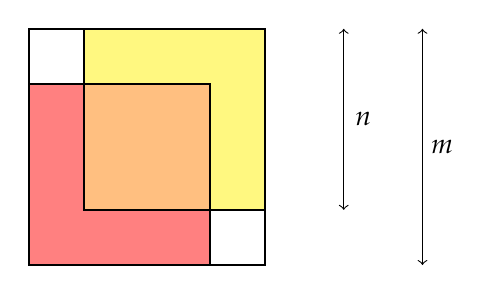
\begin{tikzpicture}
		\draw[thick] (0,0) rectangle (3,3);
		\draw[thick, fill=red!50] (0,0) rectangle (2.3,2.3);
		\draw[thick, fill=yellow!50] (0.7,0.7) rectangle (3, 3);
		\draw[thick, fill=orange!50] (0.7,0.7) rectangle (2.3, 2.3);
		\draw[<->] (4, 0.7)--(4, 3);
		\node at (4.25, 1.85) (n) {$n$};
		\draw[<->] (5, 0)--(5, 3);
		\node at (5.25, 1.5) (m) {$m$};
	\end{tikzpicture}
\end{center}
Omdat $m^2 = 2n^2$, heeft het gebied waarin de twee vierkanten met
zijde $n$ overlappen dezelfde oppervlakte als het gebied dat door
geen van beide vierkanten wordt bedekt. De oppervlakte van het oranje
vierkant is dus gelijk aan de som van de oppervlakten van de twee
niet-ingekleurde vierkanten. Als het oranje vierkant zijde $p$ heeft
en elk niet-ingekleurd vierkant zijde $q$, dan is $p^2 = 2q^2$. Nu is
echter $\sqrt{2} = \nicefrac{p}{q}$, waarbij $p < m$, $q < n$ en $p, q
\in \Nat$. Dit is in tegenspraak met de keuze van $m$ en $n$ als zo
klein mogelijk.
\emph{Ten tweede formeel.} Uit $m^{2} = 2n^{2}$ volgt dat $m$ even is.
(Als $x$ oneven is, is eenvoudig aan te tonen dat $x^2$ oneven is.)
Er geldt dus $m = 2r$ voor een zekere $r \in \Nat$. Omwerken geeft
$2r^2 = n^2$,
		%				\begin{align*}
		%					(2q)^{2} &= 2n^{2}\\
		%					4q^{2} &= 2n^{2}\\
		%					2q^{2} &= n^{2}
		%				\end{align*}
zodat ook $n$ even is. Zowel $m$ als $n$ is dus even, en daarom kan de
breuk $\nicefrac{m}{n}$ \emph{wel} verder worden vereenvoudigd. Dit
is een tegenspraak.
\end{proof}
Dit bewijs met een diagram voert ons ook terug naar
\olref[his][set][mythology]{sec}. Tennenbaum (1927--2006) was een door
en door moderne wiskundige. Toch is het bewijs onmiskenbaar fraai en
volledig sluitend, en doet het een beroep op meetkundige intuïtie.
Hoe dan ook zijn de reële getallen ``omvangrijker'' dan de rationale
getallen. In zekere zin vertonen de rationale getallen ``gaten'', die
door de reële getallen worden opgevuld. Weierstrass zag in dat dit één
eigenschap van de reële getallen beschrijft die ze van de rationale
getallen onderscheidt, namelijk de volledigheidseigenschap:
\emph{Iedere niet-lege verzameling reële getallen met een bovengrens
heeft een kleinste bovengrens.}
Het is eenvoudig in te zien dat de rationale getallen de
volledigheidseigenschap niet hebben. Beschouw bijvoorbeeld de
verzameling rationale getallen kleiner dan $\sqrt{2}$:
\[
	\Setabs{p \in \Rat}{p^2 < 2 \text{ of }p < 0}
\]
Deze verzameling heeft een rationale bovengrens; al haar !!{element}en
zijn bijvoorbeeld kleiner dan $3$. Maar wat is haar kleinste
bovengrens? We zouden `$\sqrt{2}$' willen antwoorden, maar we hebben
zojuist gezien dat $\sqrt{2}$ \emph{niet} rationaal is. Er bestaat ook
geen \emph{kleinste} rationaal getal groter dan $\sqrt{2}$. De
verzameling heeft dus wel een bovengrens, maar geen kleinste
bovengrens. De rationale getallen missen bijgevolg de
volledigheidseigenschap.
Het continuüm zou daarentegen, intuïtief bezien, de
volledigheidseigenschap moeten hebben. We willen niet alleen dat
$\sqrt{2}$ een reëel getal is, maar ook dat alle ``gaten'' in de
rationale getallenlijn worden opgevuld. Het continuüm zelf moet dus
geen ``gaten'' bevatten. Dat is precies wat volledigheid ons zal geven.
% END ACCEPTED BODY OLP-0044
\endgroup
% END ACCEPTED UNIT OLP-0044

% BEGIN ACCEPTED UNIT OLP-0045 path=translations/nl-standard/content/sets-functions-relations/arithmetization/cuts.tex source-sha256=b0b3818d5212027aa9f28128748c56409af8ac5d06a0657370f2198a084ff107
\begingroup
\def\olfilename{OLP-0045}
\def\olfilepath{content/sets-functions-relations/arithmetization/}
\hypertarget{unit-OLP-0045}{}
\typeout{PARTIAL-READER-UNIT OLP-0045}
% BEGIN ACCEPTED BODY OLP-0045 body-sha256=581badad3e1065052d49799f80083ffcfa5e80079976d56929f2de022ef70d59
% Part: sets-functions-relations
% Chapter: arithmetization
% Section: cuts
%


\olfileid{sfr}{arith}{cuts}
\olsection{Van $\Rat$ naar $\Real$}
In wezen laat de volledigheidseigenschap zien dat elk punt $\alpha$ op
de getallenlijn die lijn precies in twee helften verdeelt: een
onderste helft waarvan $\alpha$ de kleinste bovengrens is en een
bovenste helft waarvan $\alpha$ de grootste ondergrens is. Om de reële
getallen uit de rationale getallen te \emph{construeren}, stelde
Dedekind voor de reële getallen eenvoudig op te vatten als de
\emph{sneden} die de rationale getallen verdelen. We identificeren
$\sqrt{2}$ dus met de \emph{snede} die de rationale getallen
$< \sqrt{2}$ scheidt van de rationale getallen $> \sqrt{2}$.
Laten we dit nauwkeurig formuleren. Als we de rationale getallen in
twee helften verdelen, wordt de gemaakte verdeling al eenduidig bepaald
door haar \emph{onderste} helft. Dit leidt tot de volgende definitie:
\begin{defn}[Snede]
Een \emph{snede} $\alpha$ is een niet-leeg echt beginstuk van de
rationale getallen zonder grootste element. Met andere woorden,
$\alpha$ is een snede dan en slechts dan als:
\begin{enumerate}
	\item \emph{niet-leeg en echt}: $\emptyset \neq \alpha \subsetneq \Rat$
	\item \emph{beginstuk}: voor alle $p,q \in \Rat$ geldt: als $p < q \in \alpha$, dan $p \in \alpha$
	\item \emph{geen maximum}: voor elke $p \in \alpha$ bestaat er een $q \in \alpha$ waarvoor $p < q$
\end{enumerate}
Dan is $\Real$ de verzameling van alle sneden.
\end{defn}
We kunnen nu dus schrijven: $\sqrt{2} = \Setabs{p \in \Rat}{p^2 < 2\text{ of }p < 0}$. Natuurlijk moeten we nog nagaan dat dit inderdaad een
\emph{snede} is, maar dat stellen we uit tot \olref[check]{sec}.
Nu deze objecten zijn gedefinieerd, moeten we, net als eerder, de
elementaire functies en relaties erop definiëren. We beginnen met een
eenvoudig geval:
\begin{align*}
	\alpha \leq \beta \text{ dan en slechts dan als }\alpha \subseteq \beta
\end{align*}
Met deze ordening kunnen we het centrale resultaat \emph{formuleren}:
de verzameling sneden heeft de volledigheidseigenschap. Volledig
uitgeschreven luidt de uitspraak als volgt. Als $S$ een niet-lege
verzameling sneden met een bovengrens is, dan heeft $S$ een kleinste
bovengrens. Preciezer: er is een snede $\lambda$ die een bovengrens van
$S$ is, oftewel\ $(\forall \alpha \in S)\alpha \subseteq
\lambda$, en $\lambda$ is de kleinste van zulke sneden, oftewel\ $(\forall \beta \in \Real)((\forall \alpha \in S)\alpha \subseteq \beta \lif \lambda \subseteq \beta)$. Het
bewijs luidt als volgt:
\begin{thm}\ollabel{realcompleteness}
De verzameling sneden heeft de volledigheidseigenschap.
\end{thm}
\begin{proof}
Zij $S$ een willekeurige niet-lege verzameling sneden met een
bovengrens. Stel $\lambda = \bigcup S$.
%\Setabs{p \in \Rat}{(\exists \alpha \in S)p \in \alpha}$$
We beweren eerst dat $\lambda$ een snede is:
\begin{enumerate}
\item Omdat $S$ niet leeg is, bevat $S$ ten minste één snede,
dus $\emptyset \neq \lambda$. Omdat $S$ een verzameling sneden is,
geldt $\lambda \subseteq \Rat$. Omdat $S$ een bovengrens heeft, is er
een $p \in \Rat$ die in geen enkele snede $\alpha \in S$ voorkomt. Dus
$p\notin \lambda$ en bijgevolg $\lambda \subsetneq \Rat$.
\item Stel dat $p < q \in \lambda$. Dan is er een $\alpha \in S$ met
$q \in \alpha$. Omdat $\alpha$ een snede is, geldt $p \in \alpha$.
Dus $p \in \lambda$.
\item Stel dat $p \in \lambda$. Dan is er een $\alpha \in S$ met
$p \in \alpha$. Omdat $\alpha$ een snede is, is er een $q \in
\alpha$ waarvoor $p < q$. Dus $q \in \lambda$.
\end{enumerate}
Daarmee is de bewering bewezen. Bovendien geldt duidelijk $(\forall \alpha \in S)\alpha
\subseteq \bigcup S = \lambda$, oftewel\ $\lambda$ is een bovengrens van $S$. Stel nu dat $\beta \in \mathbb{R}$ eveneens een bovengrens is, oftewel\ $(\forall \alpha \in S)\alpha \subseteq \beta$. Voor elke $p \in \Rat$ geldt: als $p \in \lambda$, dan is er een $\alpha \in S$ met $p \in \alpha$, zodat $p \in \beta$. Omdat dit voor elk rationaal getal geldt, volgt $\lambda \subseteq \beta$. Dus $\lambda$ is de \emph{kleinste} bovengrens van $S$.
\end{proof}
We hebben dus objecten die aan de volledigheidseigenschap voldoen.
Anders gezegd: onze sneden vertonen geen “gaten”. (Een verdere
“snede” in de reële in plaats van de rationale getallen zou daarom
geen interessante nieuwe objecten opleveren.)
Vervolgens moeten we bewerkingen op de reële getallen definiëren. We
beginnen met een inbedding van de rationale getallen in de reële
getallen door vast te leggen dat $p_\Real =
\Setabs{q \in \Rat}{q < p}$ voor elke $p \in \Rat$. Daarna definiëren
we:
\begin{align*}
	\alpha + \beta &= \Setabs{p + q}{p \in \alpha \land q \in \beta}\\
%	\alpha - \beta &\defis \Setabs{p - q}{p \in \alpha \land q \in \Rat \setminus \beta}\\
	\alpha \times \beta &=
	\Setabs{p \times q}{0 \leq p \in \alpha \land 0 \leq q \in \beta} \cup 0_\Real & \text{als }\alpha, \beta \geq 0_\Real
%	\alpha \div \beta &\defis
%	\Setabs{\nicefrac{p}{q}}{p \in \alpha \land q \in \Rat \setminus \beta}  & \text{if }\alpha \geq 0_\Real, \beta > 0_\Real
\end{align*}
Voor ieder reëel getal leggen we bovendien vast dat nul maal dat getal
en dat getal maal nul beide nul zijn. Voor de overige gevallen van
vermenigvuldiging definiëren we eerst:
\begin{align*}
	-\alpha &= \Setabs{p - q}{p < 0 \land q \notin \alpha}
\end{align*}
en leggen we vervolgens vast:
\begin{align*}
	\alpha \times \beta &\defis
	\begin{cases}
		\mathord{-}\alpha \times \mathord{-}\beta &\text{als }\alpha < 0_\Real\text{ en }\beta < 0_\Real\\
		\mathord{-}(\mathord{-}\alpha \times \beta) &\text{als }\alpha < 0_\Real \text{ en }\beta > 0_\Real\\
		\mathord{-}(\alpha \times \mathord{-}\beta) &\text{als }\alpha > 0_\Real \text{ en }\beta < 0_\Real
	\end{cases}
\end{align*}
Vervolgens moet worden nagegaan dat elk van deze definities steeds een
snede oplevert. Ten slotte moeten we met een eenvoudig (maar omslachtig)
bewijs aantonen dat de aldus gedefinieerde sneden zich precies zo
gedragen als beoogd. Ook dit alles stellen we uit tot
\olref[check]{sec}.
% END ACCEPTED BODY OLP-0045
\endgroup
% END ACCEPTED UNIT OLP-0045

% BEGIN ACCEPTED UNIT OLP-0046 path=translations/nl-standard/content/sets-functions-relations/arithmetization/reflections.tex source-sha256=61767a02b4c8c7147cbd51df6b18d12f93da29509a7b28142a8d3ee4813ea6bd
\begingroup
\def\olfilename{OLP-0046}
\def\olfilepath{content/sets-functions-relations/arithmetization/}
\hypertarget{unit-OLP-0046}{}
\typeout{PARTIAL-READER-UNIT OLP-0046}
% BEGIN ACCEPTED BODY OLP-0046 body-sha256=2804ef7b84a2e89624f17796f2dc920fac7af419f0aa45916e2461f5e479e884
% Part: sets-functions-relations
% Chapter: arithmetization
% Section: reflections



\olfileid{sfr}{arith}{ref}
\olsection{Enkele filosofische beschouwingen}
Tot zover de technische details. Maar wat hebben ze opgeleverd?
In elk geval leverden ze {fraaie} zuivere wiskunde op. Daarnaast waren
er diepgaande begripsmatige resultaten. Het inzicht dat de
volledigheidseigenschap het wezenlijke verschil tussen de reële en de
rationale getallen uitdrukt, was diepgaand. Bovendien geeft de
expliciete constructie van de reële getallen als Dedekindsneden de
analyse een stevige grondslag. We weten dat een \emph{volledig
geordend lichaam} kan bestaan, want de sneden vormen zo'n lichaam.
Toch zijn bij deze resultaten enkele kanttekeningen op hun plaats.
Ten eerste is het niet duidelijk dat reële getallen als sneden
opvatten \emph{strenger} is dan ze opvatten via hun vertrouwde,
mogelijk oneindige decimaalontwikkelingen. Die laatste ``constructie''
van de reële getallen lijkt enigszins op de constructie met
Cauchyrijen, maar was in wezen al vanaf het begin van de zeventiende
eeuw bij wiskundigen bekend (zie \olref[cauchy]{sec}). De werkelijke
toename in strengheid kwam door het inzicht dat de reële getallen de
volledigheidseigenschap hebben. Dat we reële getallen als bepaalde
verzamelingen kunnen construeren, is op zichzelf wellicht niet zo
interessant.
Nog minder duidelijk is dat de veel eenvoudigere aritmetisering van de
gehele of rationale getallen de wiskundige behandeling ervan strenger maakt.
Hierbij is een eenvoudige vaststelling van belang. Nadat we de gehele
getallen als equivalentieklassen van geordende paren natuurlijke
getallen hebben \emph{geconstrueerd}, vervolgens de rationale getallen
als equivalentieklassen van geordende paren gehele getallen en ten
slotte de reële getallen als verzamelingen rationale getallen, gaan we
die constructies onmiddellijk weer \emph{vergeten}. Niemand zal tijdens
een wiskundig bewijs op deze constructies willen \emph{teruggrijpen},
behalve natuurlijk in een bewijs dat ze zich gedragen zoals bedoeld.
Het is veel eenvoudiger om rechtstreeks over een reëel getal te
spreken dan over een verzameling van verzamelingen van verzamelingen
van verzamelingen van verzamelingen van verzamelingen van verzamelingen
natuurlijke getallen.
%(For reals were constructed as sets of rationals; and these were constructed as equivalence classes of ordered pairs of integers, i.e., sets of sets of sets of integers; etc.).
%2/3 = [2,3]
%	i.e. {<2,3>, ... }
%	{ {{2},{2,3}}, ... }
%
%reals are 
%	sets of rationals 
%
%rationals are 
%	sets of sets of sets of integers
%
%integers are
%	sets of sets of sets of naturals
Het twijfelachtigst is dat deze definities ons vertellen wat de gehele,
rationale of reële getallen \emph{zijn}, \emph{metafysisch gezien}.
Het is dus twijfelachtig of de reële getallen bijvoorbeeld
\emph{identiek zijn aan} bepaalde verzamelingen van verzamelingen van
verzamelingen\ldots.
Het voornaamste bezwaar is dat de constructie op veel verschillende
manieren had kunnen worden uitgevoerd. Voor de reële getallen bestaan
enkele werkelijk interessante alternatieve constructies (zie
\olref[cauchy]{sec}). Maar er is ook een volkomen triviale manier om
andere constructies te krijgen. Zoals in
\olref[sfr][rel][ref]{sec} hadden we geordende paren iets anders kunnen
definiëren. Met dat alternatieve begrip van een geordend paar zouden
onze constructies even goed hebben gewerkt, maar andere objecten hebben
opgeleverd. Er bestaan dus verscheidene concurrerende constructies
binnen de verzamelingenleer van de gehele, rationale en reële
getallen. Het zou willekeurig en gênant zijn om te beweren dat de
gehele getallen bijvoorbeeld \emph{deze} verzamelingen zijn en niet
\emph{die}. (Net als in \olref[sfr][rel][ref]{sec} is dit een geval van
een argument dat door \citealt{Benacerraf1965} bekend is geworden.)
Er is nog een punt: onze constructies hebben iets uitgesproken
\emph{vreemds}. We begonnen met de natuurlijke getallen. Daarna
construeren we de gehele getallen, waaronder ``de $0$ van de gehele
getallen'', namelijk $ \equivrep{0,0}{\Intequiv}$. Maar $0 \neq
\equivrep{0,0}{\Intequiv}$. Volgens onze constructies is zelfs
\emph{geen enkel} natuurlijk getal een geheel getal. Dat lijkt zeer
tegenintuïtief. In \olref[sfr][set][imp]{sec} beweerden we immers
zonder veel toelichting dat $\Nat \subseteq \Rat$. Als de constructies
ons precies vertellen \emph{wat} de getallen zijn, was die bewering
evident onwaar.
Wat is dan de slotsom? Binnen een na\"ieve verzamelingenleer, waarin we
de natuurlijke getallen als gegeven aannemen, kunnen we gehele,
rationale en reële getallen als bepaalde verzamelingen
\emph{behandelen}. In die zin kunnen we de theorieën van deze objecten
in een verzamelingenleer \emph{inbedden}. De filosofische betekenis van
zo'n inbedding is echter niet zonder meer duidelijk.
Dit is natuurlijk niet het laatste woord!{} Het punt is alleen dit. Om
aan te tonen dat de aritmetisering van de reële getallen werkelijk van
groot filosofisch belang \emph{is}, is nog een aanvullend
\emph{filosofisch} argument nodig.
%Additionally: for the entire duration of this chapter, we have treated
%the natural numbers as simply \emph{given} to us. But what can we do
%with them? That is the subject matter for the next chapter.
% END ACCEPTED BODY OLP-0046
\endgroup
% END ACCEPTED UNIT OLP-0046

% BEGIN ACCEPTED UNIT OLP-0047 path=translations/nl-standard/content/sets-functions-relations/arithmetization/checking-details.tex source-sha256=ce1a4dbffeb56b31e9fbebbe2f9cba28c337d5dc7e2a2b1b620a95824d30f3b9
\begingroup
\def\olfilename{OLP-0047}
\def\olfilepath{content/sets-functions-relations/arithmetization/}
\hypertarget{unit-OLP-0047}{}
\typeout{PARTIAL-READER-UNIT OLP-0047}
% BEGIN ACCEPTED BODY OLP-0047 body-sha256=1ebf8b15fde5d94ef5b3d4cdf2f57a10c65da36f24a5df68d365c95ebd4b49d8
% Part: sets-functions-relations
% Chapter: arithmetization
% Section: checking-details
%


	
\olfileid{sfr}{arith}{check}
\olsection{Geordende ringen en lichamen}
In dit hoofdstuk hebben we steeds gesteld dat bepaalde definities zich
``gedragen zoals het hoort''. In deze technische bijlage leggen we
precies uit wat we daarmee bedoelen en schetsen we hoe we kunnen
aantonen dat de definities zich inderdaad ``correct'' gedragen.
In \olref[int]{sec} definieerden we optelling en vermenigvuldiging op
$\Int$. We willen aantonen dat deze bewerkingen $\Int$, met die
definities, de structuur geven die we ervan ``verwachten''. Het gaat
hier in het bijzonder om de structuur van een commutatieve ring.
\begin{defn}
	Een \emph{commutatieve ring} is een verzameling $S$ met aangewezen elementen $0$ en $1$ en bewerkingen $+$ en $\times$, waarvoor de volgende acht formules gelden:
	\begin{align*}
		\emph{Associativiteit}&&a + (b+ c) & = (a + b) + c \\
		&& (a \times b) \times c & = a \times (b\times c)\\
		\emph{Commutativiteit}&&a + b &= b+ a  \\
		&&  a \times b&= b\times a\\ 
		\emph{Neutrale elementen}&&a + 0 &= a \\
		&& a \times 1 &= a\\
		\emph{Additieve inverse}&&(\exists b\in S)0&=a + b\\
		\emph{Distributiviteit}&&a \times (b+ c ) &= (a \times b) + (a \times c)
	\end{align*}
	Stilzwijgend zijn deze formules allemaal universeel gekwantificeerd, waarbij de variabelen alleen waarden in $S$ aannemen. Merk ook op dat de elementen $0$ en~$1$ hier niet de gelijknamige natuurlijke getallen hoeven te zijn.
\end{defn}
Om aan te tonen dat de gehele getallen een commutatieve ring vormen,
hoeven we dus alleen deze acht voorwaarden te verifiëren. Geen ervan
is moeilijk te bewijzen, maar alle controles samen kosten enig werk.
Zo bewijzen we de \emph{associativiteit} van de optelling als volgt:
\begin{proof} 
Neem $i, j, k \in \Int$. Er bestaan dan $a_1, b_1, a_2, b_2, a_3, b_3 \in
\Nat$ waarvoor $i = \equivrep{a_1, b_1}{}$ en $j =
\equivrep{a_2,b_2}{}$ en $k = \equivrep{a_3, b_3}{}$. (Om de
notatie leesbaar te houden, schrijven we ``$\equivrep{x, y}{}$'' in plaats van
``$\equivrep{x, y}{\Intequiv}$''; dit doen we in de hele
paragraaf.) Dan geldt:
\begin{align*}
	i + (j + k) &= \equivrep{a_1, b_1}{}+(\equivrep{a_2, b_2}{} + \equivrep{a_3, b_3}{}) \\
	&= \equivrep{a_1,  b_1}{} + \equivrep{a_2+a_3, b_2+b_3}{}\\
	&= \equivrep{a_1 + (a_2 + a_3), b_1 + (b_2 + b_3)}{}\\
	&= \equivrep{(a_1 + a_2) + a_3, (b_1 + b_2) + b_3}{}\\
	&= \equivrep{a_1 + a_2, b_1 + b_2}{} + \equivrep{a_3, b_3}{}\\
	&= (\equivrep{a_1, b_1}{} + \equivrep{a_2, b_2}{}) + \equivrep{a_3, b_3}{}\\
	&= (i+j) + k
\end{align*}
waarbij we zonder meer de eigenschappen van de optelling op $\Nat$
gebruiken.
\end{proof}
Op dezelfde manier bewijzen we de \emph{additieve inverse}:
\begin{proof}
Neem $i \in \Int$, zodat $i = \equivrep{a,b}{}$ voor zekere $a,b \in
\Nat$. Stel $j = \equivrep{b,a}{} \in \Int$. Uit de eigenschappen van
de natuurlijke getallen volgt $(a+b) + 0 = 0 + (b+a)$, zodat
$\tuple{a+b, b+a} \sim_\Int \tuple{0,0}$ krachtens de definitie, en dus
$\equivrep{a+b, b+a}{} = \equivrep{0, 0}{} = 0_\Int$. Bijgevolg is $i + j =
\equivrep{a,b}{}+\equivrep{b,a}{}=\equivrep{a+b, b+a}{}= \equivrep{0,
0}{} = 0_\Int$.
\end{proof}
En dit is een bewijs van de \emph{distributiviteit}:
\begin{proof}
Neem, zoals hierboven, $i = \equivrep{a_1, b_1}{}$ en $j =
\equivrep{a_2,b_2}{}$ en $k = \equivrep{a_3, b_3}{}$. Dan geldt:
\begin{align*}
	i \times (j + k) 
	&= \equivrep{a_1, b_1}{} \times (\equivrep{a_2,b_2}{} + \equivrep{a_3, b_3}{})\\
	&= \equivrep{a_1, b_1}{} \times \equivrep{a_2 + a_3,b_2+b_3}{}\\
	&= \equivrep{a_1  (a_2 + a_3) + b_1  (b_2+b_3), a_1  (b_2 + b_3) + b_1 (a_2 + a_3)}{}\\
	&= \equivrep{a_1 a_2 + a_1a_3 + b_1 b_2+b_1b_3, a_1 b_2 + a_1b_3 + a_2b_1 + a_3b_1}{}\\		
%		&= \equivrep{a_1 a_2 + b_1b_2 + a_1a_3 + b_1 b_2+b_1b_3, a_1 b_2 + a_1b_3 + a_2b_1 + a_3b_1}{}\\		
	&= \equivrep{a_1a_2 + b_1b_2, a_1b_2 + a_2b_1}{} + \equivrep{a_1a_3 + b_1b_3, a_1b_3 + a_3b_1}{}\\
	&= (\equivrep{a_1, b_1}{} \times \equivrep{a_2,b_2}{}) + (\equivrep{a_1, b_1}{} \times  \equivrep{a_3, b_3}{})\\
	&= (i \times j) + (i \times k)
\end{align*}
\end{proof}
Het bewijs van de overige vijf voorwaarden laten we als oefening.
Daarmee is aangetoond dat $\Int$ een commutatieve ring vormt, oftewel
dat optelling en vermenigvuldiging zich met de gegeven definities
gedragen zoals het hoort.
\begin{prob}
Bewijs dat $\Int$ een commutatieve ring is.
\end{prob}
Daarmee zijn we nog niet klaar. Naast optelling en vermenigvuldiging
op $\Int$ hebben we een ordeningsrelatie $\leq$ gedefinieerd; ook
daarvan moeten we controleren of die de gewenste eigenschappen
heeft. Preciezer: we moeten aantonen dat $\Int$ een \emph{geordende}
ring vormt.\footnote{Bedenk dat volgens
	\olref[sfr][rel][ord]{def:linearorder} een totale ordening
	een reflexieve, transitieve, antisymmetrische en samenhangende relatie is.
	Bij ordeningsrelaties wordt samenhangendheid soms
	\emph{trichotomie} genoemd, aangezien voor alle $a$ en $b$ geldt dat $a \leq b \lor a
	= b \lor a \geq b$.} 
\begin{defn}
Een \emph{geordende ring} is een commutatieve ring die bovendien is
voorzien van een totale ordening $\leq$, zodanig dat:
\begin{align*}
	a \leq b &\lif a + c \leq b + c\\
	(a \leq b \land 0 \leq c) &\lif a \times c \leq b \times c
\end{align*}
\end{defn}
\begin{prob}
Bewijs dat $\Int$ een geordende ring is. 
\end{prob}
Net als hierboven is het bewerkelijk maar routineus om aan te tonen
dat de geconstrueerde $\Int$ een geordende ring vormt. We laten dit
aan de lezer over.
Daarmee zijn de gehele getallen afgehandeld. Voor de rationale
getallen moeten we nu zeer vergelijkbare eigenschappen aantonen. We
moeten met name laten zien dat de rationale getallen een geordend
\emph{lichaam} vormen, uitgaande van onze definities van $+$,
$\times$ en $\leq$:
\begin{defn}\ollabel{orderedfield}
Een \emph{geordend lichaam} is een geordende ring waarvoor bovendien geldt:
\begin{align*}
	\emph{Multiplicatieve inverse}& & (\forall a \in S \setminus \{0\})(\exists b \in S) a\times b& = 1
\end{align*}
\end{defn}
Wanneer eenmaal is aangetoond dat $\Int$ een geordende ring vormt, is
het eenvoudig maar bewerkelijk om aan te tonen dat $\Rat$ een
geordend lichaam vormt.
\begin{prob}
Bewijs dat $\Rat$ een geordend lichaam is.
\end{prob}
Na de gehele en rationale getallen resteren alleen de reële getallen.
We moeten in het bijzonder aantonen dat $\Real$ een \emph{volledig}
geordend lichaam vormt, dat wil zeggen een geordend lichaam met de
volledigheidseigenschap. In \olref[cuts]{realcompleteness} is al
bewezen dat $\Real$ de volledigheidseigenschap heeft. We moeten echter
nog de (saaie) controles doorlopen die aantonen dat $\Real$ een
geordend lichaam is.
Voordat we aan \emph{die} bewerkelijke oefening beginnen, moeten we
nog enkele directere zaken controleren. Zo moeten we nagaan of
$\alpha + \beta$ volgens de definitie inderdaad een \emph{snede}
is, voor willekeurige sneden $\alpha$ en $\beta$. Dit bewijzen we als
volgt:
\begin{proof}	
Omdat $\alpha$ en $\beta$ beide sneden zijn, is $\alpha + \beta = \Setabs{p
+ q}{p \in \alpha \land q \in \beta}$ een niet-lege echte deelverzameling van
$\Rat$. Stel nu $x < p + q$ voor zekere $p \in \alpha$ en $q \in \beta$.
Dan is $x - p < q$, dus $x - p \in \beta$, en $x = p + (x - p) \in
\alpha + \beta$. Bijgevolg is $\alpha + \beta$ een beginstuk van $\Rat$.
Neem ten slotte een willekeurige $p + q \in \alpha + \beta$. Omdat
$\alpha$ en $\beta$ beide sneden zijn, bestaan er $p_1 \in \alpha$ en $q_1 \in \beta$
waarvoor $p < p_1$ en $q < q_1$; derhalve is $p + q < p_1 + q_1 \in \alpha +
\beta$; dus heeft $\alpha + \beta$ geen maximum.
\end{proof}
Op soortgelijke wijze kan worden aangetoond dat $\alpha - \beta$,
$\alpha \times \beta$ en $\alpha \div \beta$ sneden zijn (bij deling
met uitzondering van het geval waarin $\beta$ de nulsnede is). Ook
dit laten we aan de lezer over.
\begin{prob}
Bewijs dat $\Real$ een geordend lichaam is.
\end{prob}
Er rest nog een kleinigheid. In \olref[cuts]{sec} stellen we voor
$\sqrt{2} = \Setabs{p \in \Rat}{p < 0 \text{ of }p^2 < 2}$ te nemen.
We moeten echter wel aantonen dat deze verzameling een \emph{snede}
is. Dit bewijs luidt als volgt:
\begin{proof}
Dit is duidelijk een niet-leeg echt beginstuk van de rationale
getallen; het volstaat dus aan te tonen dat het geen maximum heeft.
Meer bepaald volstaat het aan te tonen dat voor elk positief
rationaal getal $p$ met $p^2 < 2$ en $q = \frac{2p+2}{p+2}$ zowel $p
< q$ als $q^2 < 2$ geldt. Voor $p < q$ geldt:
\begin{align*}
	p^2 &< 2\\
	p^2 + 2p &< 2 + 2p\\
	p(p + 2) &< 2 + 2p\\
	p &< \tfrac{2+2p}{p+2} = q
\end{align*}
Voor $q^2 < 2$ geldt:
\begin{align*}
	p^2 &< 2\\
	2p^2 + 4p + 2 &< p^2 + 4p+ 4\\
	4p^2 + 8p + 4 &< 2(p^2 + 4p + 4)\\
	(2p+2)^2 & <2(p+2)^2\\
	\tfrac{(2p+2)^2}{(p+2)^2} &< 2\\
	q^2 &< 2
\end{align*}
\end{proof}
% END ACCEPTED BODY OLP-0047
\endgroup
% END ACCEPTED UNIT OLP-0047

% BEGIN ACCEPTED UNIT OLP-0048 path=translations/nl-standard/content/sets-functions-relations/arithmetization/cauchy.tex source-sha256=c32c88da4ec103ae9f3389f5d543f21897e307f8a46d717efedbe717f64901be
\begingroup
\def\olfilename{OLP-0048}
\def\olfilepath{content/sets-functions-relations/arithmetization/}
\hypertarget{unit-OLP-0048}{}
\typeout{PARTIAL-READER-UNIT OLP-0048}
% BEGIN ACCEPTED BODY OLP-0048 body-sha256=1f3c3be0a1c1b9e28a7332a56b3f77a368a2112a1766c3d339cc5f891ac3faeb
% Part: sets-functions-relations
% Chapter: arithmetization
% Section: cauchy



\olfileid{sfr}{arith}{cauchy}
\olsection{Bijlage: de reële getallen als Cauchyrijen}
In \olref[cuts]{sec} hebben we de reële getallen geconstrueerd als
Dedekindsneden. In deze paragraaf leggen we een alternatieve
constructie uit. Die berust op Cauchy's definitie van wat we nu een
Cauchyrij noemen. Het gebruik van deze definitie om de reële getallen
te \emph{construeren} is echter afkomstig van andere negentiende-eeuwse
auteurs, met name Weierstrass, Heine, M\'{e}ray en Cantor. (Voor een
helder historisch overzicht, zie \citeauthor{OConnorRobertson:RN}
\citeyear{OConnorRobertson:RN}.)
Voordat we de negentiende eeuw behandelen, staan we stil bij Simon
Stevin (1548--1620). Stevin zag dat we elk reëel getal kunnen opvatten
via zijn decimaalontwikkeling. Zelfs een irrationaal getal als
$\sqrt{2}$ heeft dus een nette decimaalontwikkeling, die als volgt
begint:
\[
	1.41421356237\ldots
\] 
Decimaalontwikkelingen zijn eenvoudig in de verzamelingenleer te
modelleren: beschouw ze als functies $d \colon \Nat \to \Nat$, waarbij
$d(n)$ het $n$-de cijfer achter de komma is dat ons interesseert. Er is
dan een kleine aanpassing nodig voor het deel van het reële getal vóór
de komma (hier alleen $1$). Ook is een tweede aanpassing nodig, in de
vorm van een equivalentierelatie, om bijvoorbeeld te waarborgen dat
$0.999\ldots = 1$. Op deze manier kan binnen de verzamelingenleer zonder
veel moeite een volledig strenge constructie van de reële getallen in
de trant van Stevin worden gegeven.
Stevin is hier niet ons onderwerp. (Zie voor meer over Stevin
\citealt{KatzKatz2012}.) Wel gebruiken we een nauw verwant idee. In
plaats van de decimaalontwikkeling van $\sqrt{2}$ rechtstreeks te
beschouwen, kunnen we een \emph{rij} steeds nauwkeurigere rationale
benaderingen van $\sqrt{2}$ nemen, via de steeds preciezere
decimaalbenaderingen:
\[
1, 1.4, 1.414, 1.4142, 1.41421,\ldots
\]
Het idee dat reële getallen via ``steeds betere benaderingen'' kunnen
worden beschouwd, vormt de basis voor een nieuwe reeks inzichten. Ze
lijken op de inzichten waarmee we $\Rat$ uit $\Int$ en $\Int$ uit
$\Nat$ hebben geconstrueerd. Het gaat om het volgende:
\begin{enumerate}
	\item Elk reëel getal kan als een mogelijk oneindige
	decimaalontwikkeling worden geschreven.
	\item De informatie in zo'n mogelijk oneindige decimaalontwikkeling
	kan evengoed in een rij rationale getallen worden vastgelegd.
	\item Een rij rationale getallen kan worden opgevat als een functie
	van $\Nat$ naar $\Rat$: laat $f(n)$ eenvoudig het $n$-de rationale
	getal in de rij zijn.
\end{enumerate}
Niet \emph{elke} functie van $\Nat$ naar $\Rat$ levert echter een reëel
getal op. Beschouw bijvoorbeeld de functie:
\[
	f(n) =\begin{cases}
			1 & \text{als }n\text{ oneven is}\\
			0 &\text{als }n\text{ even is}
		\end{cases}
\]
Het probleem is dat de rij $0,1,0,1,0,1,0,\ldots$ geen enkel reëel
getal lijkt te benaderen. Om alleen rijen te beschouwen die wel een
reëel getal benaderen, beperken we ons daarom tot rijen met een
\emph{limiet}.
In \olref[his][set][limits]{sec} zijn we het begrip limiet al
tegengekomen. We kunnen hier echter niet \emph{precies} dezelfde
definitie gebruiken. De uitdrukking ``$(\forall \epsilon>0)$'' bevatte
daar stilzwijgend een kwantificatie over de reële getallen, en we
beschouwden limieten van functies op de reële getallen. Die definitie
gebruiken zou dus betekenen dat we de reële getallen al aannemen,
terwijl we juist die getallen willen \emph{construeren}. Gelukkig
kunnen we met een nauw verwant limietbegrip werken.
\begin{defn}\ollabel{def:CauchySequence}
  Een functie $f: \Nat \to \Rat$ is een \emph{Cauchyrij} dan en slechts
  dan als voor elke positieve $\epsilon \in \Rat$ geldt dat $(\exists
  \ell \in \Nat)(\forall m, n > \ell)|f(m) - f(n)| < \epsilon$.
\end{defn}
Het algemene limietidee is hetzelfde als voorheen. Voor elk gewenst
nauwkeurigheidsniveau, gemeten door~$\epsilon$, is er een ``gebied''
waarin we moeten kijken: alle invoeren groter dan~$\ell$. Onze rij
$1$, $1.4$, $1.414$, $1.4142$, $1.41421$\ldots heeft duidelijk een
limiet. Wie $\sqrt{2}$ wil benaderen met een fout kleiner dan
$\nicefrac{1}{10^{n}}$, kan elke term na de $n$-de nemen.
Een voor de hand liggende gedachte is dan dat elk reëel getal gewoon
een Cauchyrij \emph{is}. Net als bij de constructies van $\Int$ en
$\Rat$ zou dat te na\"ief zijn: hetzelfde reële getal wordt door
verschillende Cauchyrijen aangegeven. Dat is eenvoudig te zien. Neem
een Cauchyrij~$f$ en definieer $g$ als precies dezelfde functie als~$f$,
behalve dat $g(0)\neq f(0)$. Na de eerste term zijn de twee rijen
overal gelijk. Uiteindelijk willen we daarom zeggen dat ze dezelfde
limiet hebben, in de betekenis van \olref{def:CauchySequence}, en dus
hetzelfde reële getal ``definiëren''. We moeten deze Cauchyrijen dus als
hetzelfde reële getal beschouwen.
Daarom moeten we opnieuw een equivalentierelatie op de Cauchyrijen
definiëren en reële getallen met equivalentieklassen van Cauchyrijen identificeren.
Eerst hebben we het begrip nodig van een functie die in de limiet naar
$0$ gaat. Voor elke functie $h : \Nat \to \Rat$ zeggen we dat
\emph{$h$ naar $0$ gaat} dan en slechts dan als voor elke positieve
$\epsilon \in \Rat$ geldt dat $(\exists \ell \in \Nat)(\forall n >
\ell)|h(n)| < \epsilon$.\footnote{Vergelijk dit met de definitie van
$\lim_{x \mathord{\rightarrow}\infty}f(x) = 0$ in
\olref[his][set][limits]{sec}.} Zijn $f$ en $g$ functies $\Nat \to
\Rat$, stel dan $(f-g)(n) = f(n) - g(n)$. Definieer nu:
\[
	f \Realequiv g \text{ dan en slechts dan als $(f-g)$ naar $0$ gaat}.
\]
We moeten controleren dat $\Realequiv$ een equivalentierelatie is, en
dat is inderdaad zo. Vervolgens kunnen we de reële getallen desgewenst
definiëren als de equivalentieklassen onder $\Realequiv$ van alle
Cauchyrijen van $\Nat \to \Rat$.
\begin{prob}
Stel $f(n) = 0$ voor elke $n$. Stel $g(n) = \frac{1}{(n+1)^2}$. Toon
aan dat beide Cauchyrijen zijn en dat beide functies inderdaad limiet
$0$ hebben, zodat ook $f \sim_\Real g$.
\end{prob}
Zoals gebruikelijk schrijven we nu $\equivrep{f}{\Realequiv}$ voor de
equivalentieklasse met $f$ als !!a{element}. Voor de leesbaarheid laten
we de index hierna echter weg en schrijven we alleen
$\equivrep{f}{}$. Verder spreken we af dat voor elke $q \in \Rat$
geldt: $q_{\Real} = \equivrep{c_{q}}{}$, waarbij $c_{q}$ de constante
functie is met $c_q(n) = q$ voor alle $n \in \Nat$. Vervolgens
definiëren we de elementaire relaties en bewerkingen op de reële
getallen, bijvoorbeeld:
\begin{align*}
	\equivrep{f}{} + \equivrep{g}{} &= 	\equivrep{(f + g)}{} \\
	\equivrep{f}{} \times 	\equivrep{g}{} &= \equivrep{(f \times g)}{} 
\end{align*}
waarbij $(f + g)(n) = f(n) + g(n)$ en $(f \times g)(n) = f(n) \times
g(n)$. Ook moeten we controleren dat $(f + g)$, $(f-g)$ en $(f\times
g)$ Cauchyrijen zijn wanneer $f$ en $g$ dat zijn. Dat is inderdaad zo;
we laten het bewijs aan de lezer.
Ten slotte definiëren we een ordening. We noemen $\equivrep{f}{}$
\emph{positief} dan en slechts dan als zowel $\equivrep{f}{}\neq
0_\Real$ als $(\exists \ell \in \Nat)(\forall n > \ell)0 < f(n)$
geldt. Vervolgens definiëren we $\equivrep{f}{} < \equivrep{g}{}$ dan
en slechts dan als $\equivrep{(g - f)}{}$ positief is. We moeten
controleren dat dit welgedefinieerd is, dus niet afhangt van de keuze
van de ``representerende'' functie uit de equivalentieklasse.
%\begin{align*}
%	\equivrep{f}{} \leq \equivrep{g}{} \text{ iff }&\equivrep{f}{} = \equivrep{g}{} \text{ or }\\
%	&(\exists \ell \in \Nat)(\forall n \in \Nat)(\ell < n \lif f(n) \leq g(n))
%\end{align*}
Daarna is vrij eenvoudig aan te tonen dat deze definities de juiste
algebraïsche eigenschappen opleveren:
\begin{thm}\ollabel{thm:cauchyorderedfield}
De Cauchyrijen vormen een geordend lichaam.
\end{thm}
\begin{proof}
Oefening.
\end{proof}
\begin{prob}
Bewijs dat de Cauchyrijen een geordend lichaam vormen.
\end{prob}
Het is moeilijker te bewijzen dat de aldus geconstrueerde reële
getallen de volledigheidseigenschap hebben. Daarom geven we dat bewijs.
\begin{thm}
Elke niet-lege verzameling Cauchyrijen met een bovengrens heeft een
kleinste bovengrens.
\end{thm}
\begin{proof}[Bewijsschets] Zij $S$ een willekeurige niet-lege
verzameling Cauchyrijen met een bovengrens. Er is dus een $p \in \Rat$
waarvoor $p_{\Real}$ een bovengrens van $S$ is. Zij $r \in S$; dan is er
een $q \in \Rat$ waarvoor $q_{\Real} < r$. Als $S$ een kleinste
bovengrens heeft, ligt die dus tussen $q_\Real$ en $p_\Real$, met de
grenzen inbegrepen.
We sluiten de kleinste bovengrens steeds verder in door haar tegelijk
van onderen en van boven te benaderen. Daartoe definiëren we twee
functies $f, g \colon \Nat \to \Rat$, met het doel dat $f$ de kleinste
bovengrens\ van bovenaf en $g$ haar van onderaf benadert. We beginnen
met:
\begin{align*}
	f(0) &= p \\
	g(0) &= q
\end{align*}
Stel vervolgens $a_n = \frac{f(n) + g(n)}{2}$ en
definieer:\footnote{Dit is een recursieve definitie. We hebben echter
\emph{nog} geen reden gegeven om aan te nemen dat recursieve definities
toelaatbaar zijn.}
\begin{align*}
	f(n+1) &=
	\begin{cases}
		a_n &\text{als }(\forall h \in S)\equivrep{h}{} \leq (a_n)_\Real\\
		f(n)&\text{anders}
	\end{cases}\\
	g(n+1) &=
	\begin{cases}
		a_n &\text{als }(\exists h \in S)\equivrep{h}{} \geq (a_n)_\Real\\
	 	g(n) &\text{anders}
	\end{cases}
\end{align*}
Zowel $f$ als $g$ is een Cauchyrij. (Dit is vrij eenvoudig te
controleren, maar we laten het als oefening.) De functie $(f-g)$ gaat
naar $0$, want het verschil tussen $f$ en $g$ is na elke stap ten
hoogste half zo groot. Dus $\equivrep{f}{} = \equivrep{g}{}$.
Eerst tonen we aan dat $\equivrep{f}{}$ een bovengrens van $S$ is,
dus:\ dat $(\forall h \in S)\equivrep{h}{} \leq \equivrep{f}{}$. (Daarbij
gebruiken we \olref{thm:cauchyorderedfield}.) Zij $h \in S$ en neem ter
tegenspraak aan dat $\equivrep{f}{} < \equivrep{h}{}$, zodat $0_\Real <
\equivrep{(h-f)}{}$. Omdat $f$ een monotoon dalende Cauchyrij is, is er
een $n \in \Nat$ waarvoor $\equivrep{(c_{f(n)} - f)}{} <
\equivrep{(h-f)}{}$. Dus:
\[
	(f(n))_\Real = \equivrep{c_{f(n)}}{} < \equivrep{f}{} + \equivrep{(h-f)}{} = \equivrep{h}{},
\]
in tegenspraak met het feit dat volgens de constructie
$\equivrep{h}{} \leq (f(n))_\Real$.
Vervolgens tonen we aan dat $\equivrep{f}{} = \equivrep{g}{}$ de
\emph{kleinste} bovengrens van $S$ is. Zij $j$ een willekeurige
Cauchyrij en neem aan dat $\equivrep{j}{} < \equivrep{g}{}$. Net als
hierboven volgt, omdat $g$ \emph{stijgend} is, dat er een $n \in \Nat$
bestaat waarvoor $\equivrep{j}{} < (g(n))_\Real$. Volgens de constructie
is er echter een $h \in S$ waarvoor $(g(n))_\Real \leq
\equivrep{h}{}$. Dus $\equivrep{j}{} < \equivrep{h}{}$, zodat
$\equivrep{j}{}$ geen bovengrens van $S$ is.
\end{proof}
% END ACCEPTED BODY OLP-0048
\endgroup
% END ACCEPTED UNIT OLP-0048
\OLEndChapterHook

% BEGIN ACCEPTED UNIT OLP-0049 path=translations/nl-standard/content/sets-functions-relations/infinite/infinite.tex source-sha256=1bce6c0b9dea42517903bbe7d7bc0ce92a50496dd3a521e2608099c55acb790e
\begingroup
\def\olfilename{OLP-0049}
\def\olfilepath{content/sets-functions-relations/infinite/}
\hypertarget{unit-OLP-0049}{}
\typeout{PARTIAL-READER-UNIT OLP-0049}
% BEGIN ACCEPTED BODY OLP-0049 body-sha256=3b1041dfc91051b3952878944b99acd82aaecad8d885835088dea5da970a2dc5
% Part: sets-functions-relations
% Chapter: infinite



\olchapter{sfr}{infinite}{Oneindige verzamelingen}

\begin{editorial}
Dit hoofdstuk over oneindige verzamelingen is overgenomen uit Tim Buttons
\emph{Open Set Theory}.
\end{editorial}
% END ACCEPTED BODY OLP-0049
\endgroup
% END ACCEPTED UNIT OLP-0049

% BEGIN ACCEPTED UNIT OLP-0050 path=translations/nl-standard/content/sets-functions-relations/infinite/hilberts-hotel.tex source-sha256=7738165ed6af0ee958ac73f933963a732e10fa2fc6f500ed48d7a0b97a18a9b2
\begingroup
\def\olfilename{OLP-0050}
\def\olfilepath{content/sets-functions-relations/infinite/}
\hypertarget{unit-OLP-0050}{}
\typeout{PARTIAL-READER-UNIT OLP-0050}
% BEGIN ACCEPTED BODY OLP-0050 body-sha256=79c6436e6cbfa3dbe635db05827f849cd24192237a8bf8646e02329379aea428
% Part: sets-functions-relations
% Chapter: infinite
% Section: hilberts-hotel
%


\olfileid{sfr}{infinite}{hilbert}
\olsection{Hilberts hotel}

De verzameling natuurlijke getallen is duidelijk oneindig. Als we de
natuurlijke getallen niet zonder meer \emph{als gegeven willen aannemen},
moeten we daarom eerst een oneindige verzameling karakteriseren zonder
de natuurlijke getallen zelf te noemen. Hilbert presenteerde hiervoor
in een voordracht uit 1924 een fraaie aanpak. Hij vraagt ons het
volgende voor te stellen:
\begin{quote}
[\ldots] een hotel met een eindig aantal kamers. Elk van deze kamers
dient door precies één gast bezet te zijn. Als de gasten nu op een of
andere manier van kamer wisselen, [maar] zodanig dat elke kamer nog
steeds hoogstens één persoon bevat, komen er geen kamers vrij en kan de
hoteleigenaar zo geen plaats maken voor een nieuw aangekomen gast [\ldots
\textparagraph \ldots]

Nu nemen we aan dat het hotel oneindig veel genummerde kamers $1$,
$2$, $3$, $4$, $5$, \dots{} heeft, die elk door precies één gast bezet
zijn. Zodra een nieuwe gast aankomt, hoeft de eigenaar slechts iedere
oude gast te verplaatsen naar de kamer met het nummer dat één hoger
ligt; kamer~$1$ is dan vrij voor de nieuw aangekomen gast.
	\begin{center}
		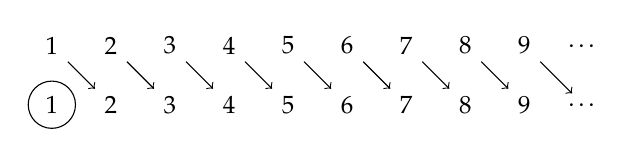
\begin{tikzpicture}[scale = .75]
		\foreach \x in {1, 2, 3, 4, 5, 6, 7, 8, 9}
		{
			\node (\x a) at (\x, 1) {\small{\x}};
			\node (\x b) at (\x, 2) {\small{\x}};
		}
		\node (dotsa) at (10, 1) {\small{\ldots}};
		\node (dotsb) at (10, 2) {\small{\ldots}};
		\draw[->] (1b)--(2a);
		\draw[->] (2b)--(3a);
		\draw[->] (3b)--(4a);
		\draw[->] (4b)--(5a);
		\draw[->] (5b)--(6a);
		\draw[->] (6b)--(7a);
		\draw[->] (7b)--(8a);
		\draw[->] (8b)--(9a);
		\draw[->] (9b)--(dotsa);
		\draw (1,1) circle (.4);
		\end{tikzpicture}
	\end{center}
	(gepubliceerd in \citealt[730]{EwaldSieg2013}; onze vertaling)
\end{quote}
Het wezenlijke punt is dat Hilberts hotel oneindig veel kamers heeft;
we kunnen zijn uitleg gebruiken om te definiëren wat dat betekent.
Dit was inderdaad Dedekinds aanpak (hier uiteraard op sterk
anachronistische wijze gepresenteerd; Dedekinds definitie dateert uit
\citeyear{Dedekind1888}):

\begin{defn}\ollabel{defn:DedekindInfinite}
Een verzameling $A$ is \emph{Dedekind-oneindig} dan en slechts dan als
er een injectie van~$A$ naar een echte deelverzameling van~$A$ bestaat.
Dat wil zeggen: er bestaan een $o \in A$ en een injectie $f \colon A
\to A$ zodanig dat $o \notin \ran{f}$.
\end{defn}
% END ACCEPTED BODY OLP-0050
\endgroup
% END ACCEPTED UNIT OLP-0050

% BEGIN ACCEPTED UNIT OLP-0051 path=translations/nl-standard/content/sets-functions-relations/infinite/dedekind-algebra.tex source-sha256=f226880951cb316b6d459e920ca27dedb0f34329684bda5c42dc2a5527ed7d6b
\begingroup
\def\olfilename{OLP-0051}
\def\olfilepath{content/sets-functions-relations/infinite/}
\hypertarget{unit-OLP-0051}{}
\typeout{PARTIAL-READER-UNIT OLP-0051}
% BEGIN ACCEPTED BODY OLP-0051 body-sha256=919ff248033b67f8c21efeb11f12aef632209951dc3fc75e6c8df821ac6a4844
% Part: sets-functions-relations
% Chapter: infinite
% Section: dedekind
%


\olfileid{sfr}{infinite}{dedekind}
\olsection{Dedekindalgebra's}

We verlangen niet alleen dat de natuurlijke getallen oneindig zijn;
ze moeten ook bepaalde (algebraïsche) eigenschappen hebben: optelling,
vermenigvuldiging enzovoort moeten zich goed gedragen.

Dedekinds idee was om de \emph{opvolgerfunctie} als uitgangspunt te
nemen en de getallen vervolgens te karakteriseren aan de hand van de
volgende eigenschappen:
\begin{enumerate}
	\item Er is een getal, $0$, dat van geen enkel getal de opvolger is
	\\d.w.z., $0 \notin \ran{s}$
	\\d.w.z., $\forall x\ s(x) \neq 0$
	\item Verschillende getallen hebben verschillende opvolgers
	\\d.w.z., $s$ is injectief
	\\d.w.z., $\forall x \forall y (s(x) = s(y) \lif x = y)$
	\item\ollabel{repeatedapplication} Elk getal wordt verkregen door de
	opvolgerfunctie herhaaldelijk op $0$ toe te passen.
\end{enumerate}
De eerste twee voorwaarden zijn eenvoudig met eerste-ordelogica te
behandelen (zie hierboven). Voor \olref{repeatedapplication} volstaat
eerste-ordelogica echter niet. Dedekinds doorbraak was om voorwaarde
\olref{repeatedapplication} als volgt in verzamelingenleer te
herformuleren:
\begin{enumerate}
	\item[3$'$.] De natuurlijke getallen vormen de kleinste verzameling
	die \emph{gesloten is onder de opvolgerfunctie}: als we $s$ op een
	willekeurig element van de verzameling toepassen, verkrijgen we
	opnieuw een element van die verzameling.
\end{enumerate}
We moeten dit echter stap voor stap uitwerken.

\begin{defn}\ollabel{Closure}
	Voor elke functie $f$ heet de verzameling $X$ $f$-\emph{gesloten}
	{dan en slechts dan als} $(\forall x \in X)f(x) \in X$. Definieer
	nu voor elke $o$:
	$$\closureofunder{f}{o} = \bigcap\Setabs{X}{o \in X\text{ en }X
\text{ $f$-gesloten is}}$$
\end{defn}

Dus $\closureofunder{f}{o}$ is de doorsnede van alle $f$-gesloten
verzamelingen die $o$ als element bevatten. Intuïtief is
$\closureofunder{f}{o}$ dan de \emph{kleinste} $f$-gesloten verzameling
die $o$ als element bevat. Het volgende resultaat maakt deze
intuïtieve gedachte precies:
\begin{lem}\ollabel{closureproperties}
	Voor elke verzameling $A$, elke functie $f \colon A \to A$ en elke
	$o \in A$:
	\begin{enumerate}
		\item\ollabel{closurehaselem} $o \in \closureofunder{f}{o}$; en
		\item\ollabel{closureclosed} $\closureofunder{f}{o}$ is $f$-gesloten; en
		\item\ollabel{closuresmallest} als $X$ $f$-gesloten is en $o \in
		X$, dan $\closureofunder{f}{o} \subseteq X$
	\end{enumerate}
\end{lem}

\begin{proof}
Er bestaat ten minste één $f$-gesloten verzameling die $o$ als element
bevat, namelijk $\ran{f}\cup \{o\}$. De verzameling
$\closureofunder{f}{o}$, de doorsnede van \emph{alle} zulke
verzamelingen, bestaat dus. Nu moeten we
\olref{closurehaselem}--\olref{closuresmallest} verifiëren.

\olref{closurehaselem} volgt omdat $o \in \closureofunder{f}{o}$: dit
is een doorsnede van verzamelingen die $o$ allemaal als element hebben.

Voor \olref{closureclosed}, stel dat $x \in \closureofunder{f}{o}$.
Als $o \in X$ en $X$ $f$-gesloten is, dan is dus $x \in X$ en ook
$f(x) \in X$, omdat $X$ $f$-gesloten is. Bijgevolg is
$f(x) \in \closureofunder{f}{o}$.

\olref{closuresmallest} volgt uit het algemene feit dat als $X \in C$,
dan $\bigcap C \subseteq X$.
\end{proof}

Hiermee kunnen we de volgende definitie geven:

\begin{defn}
Een \emph{Dedekindalgebra} bestaat uit een verzameling $A$, een functie
$f \colon A \to A$ en een element $o \in A$ waarvoor geldt:
	\begin{enumerate}
		\item \ollabel{ded:proper} $o \notin \ran{f}$
		\item \ollabel{ded:injection} $f$ is injectief
		\item \ollabel{ded:closure} $A = \closureofunder{f}{o}$
	\end{enumerate}
\end{defn}

Omdat $A = \closureofunder{f}{o}$, volgt uit ons eerdere resultaat dat
$A$ de kleinste $f$-gesloten verzameling is die $o$ als element bevat.
Een Dedekindalgebra is duidelijk Dedekind-oneindig; dit volgt direct
uit de onderdelen \olref{ded:proper} en \olref{ded:injection} van de
definitie. Belangrijker is dat elke Dedekind-oneindige verzameling tot
een Dedekindalgebra kan worden gemaakt.

\begin{thm}\ollabel{thm:DedekindInfiniteAlgebra}
Als er een Dedekind-oneindige verzameling bestaat, dan bestaat er een
Dedekindalgebra.
\end{thm}

\begin{proof}
Zij $D$ Dedekind-oneindig. Dan bestaan er een injectie $g \colon D \to
D$ en een element $o \in D \setminus \ran{g}$. Stel nu $A =
\closureofunder{g}{o}$; volgens \olref{closureproperties} bestaat $A$
en geldt $o \in A$. Stel $f = \funrestrictionto{g}{A}$. We tonen aan
dat $A, f, o$ samen een Dedekindalgebra vormen.

Voor \olref{ded:proper} geldt: $o \notin \ran{g}$ en $\ran{f}
\subseteq \ran{g}$, dus $o\notin \ran{f}$.

Voor \olref{ded:injection}: $g$ is een injectie op $D$ en $f
\subseteq g$, dus is de beperking eveneens een injectie.

Voor \olref{ded:closure}: volgens \olref{closureproperties} is $A$
$g$-gesloten; dus is $A$ zeker ook $f$-gesloten. Daarom is
$\closureofunder{f}{o} \subseteq A$ volgens
\olref{closureproperties}. Ook is $\closureofunder{f}{o}$
$f$-gesloten en geldt $f = \funrestrictionto{g}{A}$; daaruit volgt dat
$\closureofunder{f}{o}$ $g$-gesloten is. Dus
$A \subseteq \closureofunder{f}{o}$ volgens
\olref{closureproperties}.
\end{proof}
% END ACCEPTED BODY OLP-0051
\endgroup
% END ACCEPTED UNIT OLP-0051

% BEGIN ACCEPTED UNIT OLP-0052 path=translations/nl-standard/content/sets-functions-relations/infinite/dedekind-induction.tex source-sha256=43a4b1d9be0133857f7406ff64198e946ec695f747659abd187727c2010236f8
\begingroup
\def\olfilename{OLP-0052}
\def\olfilepath{content/sets-functions-relations/infinite/}
\hypertarget{unit-OLP-0052}{}
\typeout{PARTIAL-READER-UNIT OLP-0052}
% BEGIN ACCEPTED BODY OLP-0052 body-sha256=0f3462b922ca1d800f4ff09be2203b2f0ed356f0545b81317b0c35a9a06607ca
% Part: sets-functions-relations
% Chapter: infinite
% Section: dedekind-induction



\olfileid{sfr}{infinite}{induction}
\olsection[Volledige inductie]{Dedekindalgebra's en volledige inductie}

Het cruciale punt is nu dat een Dedekindalgebra---zelfs \emph{elke}
Dedekindalgebra---als vervanging voor de natuurlijke getallen kan
dienen. Dit volgt onmiddellijk uit het volgende eenvoudige resultaat:

\begin{thm}[Volledige inductie]\ollabel{thm:dedinfiniteinduction}
Laat $N, s, o$ samen een Dedekindalgebra vormen. Dan geldt voor elke
verzameling $X$:
	\begin{center}
		als $o \in X$ en $(\forall {n} \in N \cap X){s}({n}) \in X$, {dan} $N \subseteq X$.
	\end{center}
\end{thm}

\begin{proof}
Volgens de definitie van een Dedekindalgebra is $N =
\closureofunder{s}{o}$. Als zowel ${o} \in X$ als $(\forall {n} \in
N)(n \in X \lif {s}({n}) \in X)$ geldt, dan behoort het gekozen
element ook tot de onderliggende verzameling; dus geldt ${o} \in N
\cap X$. Neem nu ${n} \in N \cap X$. De aanname geeft
${s}({n}) \in X$, terwijl
${s}({n}) \in N$ omdat $s \colon N \to N$. Dus is $N \cap X$
$s$-gesloten. Deze verzameling bevat het gekozen element en bevat
daarom de kleinste dergelijke verzameling. Bijgevolg is $N =
\closureofunder{s}{o} \subseteq X$.
\end{proof}

Inductie is kenmerkend voor de natuurlijke getallen. De kern is dus dat
we uit elke Dedekind-oneindige verzameling een Dedekindalgebra kunnen
vormen en die algebra als vervanging voor de natuurlijke getallen
kunnen gebruiken.

In \olref{thm:dedinfiniteinduction} is inductie weliswaar in
\emph{verzamelingstheoretische} termen geformuleerd, maar we kunnen
het principe eenvoudig in een vertrouwder vorm weergeven:

\begin{cor}\ollabel{natinductionschema}
Laat $N, s, o$ samen een Dedekindalgebra vormen. Dan geldt voor elke
formule $\phi(x)$, waarin parameters mogen voorkomen:
\begin{center}
	als $\phi(o)$ en $(\forall {n} \in N)(\phi(n)\lif
	\phi({s}({n})))$, {dan} $(\forall n \in N)\phi(n)$
\end{center}
\end{cor}

\begin{proof}
Neem $X = \Setabs{n \in N}{\phi(n)}$ en pas nu
\olref{thm:dedinfiniteinduction} toe.
\end{proof}

In dit resultaat spraken we van een formule ``met parameters''.
Daarmee bedoelen we ruwweg dat we voor willekeurige objecten $c_1,
\ldots, c_k$ met $\phi(x, c_1, \ldots, c_k)$ kunnen werken. Preciezer
kunnen we het resultaat zonder het woord ``parameters'' als volgt
formuleren. Voor elke formule $\phi(x, v_1, \ldots, v_k)$ waarvan alle
vrije variabelen zijn weergegeven, geldt:
	\begin{align*}
			\forall v_1 \ldots \forall v_k((&\phi(o, v_1,\ldots, v_k) \land {}\\
			&	(\forall x \in N)(\phi(x,v_1, \ldots, v_k) \lif \phi(s(x), v_1,\ldots, v_k))) \lif {}\\
			&\hspace{3em} (\forall x \in N)\phi(x, v_1,\ldots, v_k))
	\end{align*}
De uitdrukking ``met parameters'' maakt een tekst dus duidelijk veel
leesbaarder. (In \olref[sth][][]{part} zullen we deze manier van spreken
vaak gebruiken.)

Terug naar Dedekindalgebra's. In elke Dedekindalgebra kunnen we ook de
gebruikelijke rekenkundige functies voor optelling, vermenigvuldiging
en machtsverheffing definiëren. Dit is echter niet triviaal: daarvoor
is de techniek van de \emph{recursieve definitie} nodig. Die techniek
zullen we pas veel later invoeren en rechtvaardigen, in een veel
algemenere context. (Wie geïnteresseerd is, kan dit na
\olref[sth][ord-arithmetic][]{chap} opnieuw bekijken, of bijvoorbeeld
een alternatieve behandeling lezen, zoals \citealt[pp.~95--8]{Potter2004}.)
Als $N, s, o$ samen een Dedekindalgebra vormen, zullen we uiteindelijk
het volgende kunnen vastleggen:
\begin{align*}
	{a} + {o} &= {a} & & & {a} \times {o} &= {o} & & & {a}^{o} &= s(o)\\
{a} + {s}({b}) &= {s}({a}+{b}) &&& {a} \times {s}({b}) &= ({a}\times {b}) + {a}  & & & {a}^{{s}({b})} &= {a}^{b} \times {a}
\end{align*}
en aantonen dat deze functies zich gedragen zoals gewenst.
% END ACCEPTED BODY OLP-0052
\endgroup
% END ACCEPTED UNIT OLP-0052

% BEGIN ACCEPTED UNIT OLP-0053 path=translations/nl-standard/content/sets-functions-relations/infinite/dedekinds-proof.tex source-sha256=d32156d8db7a9c9d48332fed35c6eaac64786a712fa51a5aabb1b8ff9ed979b1
\begingroup
\def\olfilename{OLP-0053}
\def\olfilepath{content/sets-functions-relations/infinite/}
\hypertarget{unit-OLP-0053}{}
\typeout{PARTIAL-READER-UNIT OLP-0053}
% BEGIN ACCEPTED BODY OLP-0053 body-sha256=f6aa803421b036ea47c410525b764bda4d198d248a09cab4d2775e61d6b6936d
% Part: sets-functions-relations
% Chapter: infinite
% Section: dedekinds-proof
%


\olfileid{sfr}{infinite}{dedekindsproof}

\olsection[Dedekinds ``bewijs'']{Dedekinds ``bewijs'' voor het
bestaan van een oneindige verzameling}

In dit hoofdstuk hebben we de natuurlijke getallen
verzamelingtheoretisch behandeld met behulp van Dedekindalgebra's. In
\olref[arith][ref]{sec} stonden we onder meer stil bij de filosofische
betekenis van de aritmetisering van de analyse. Nu moeten we stilstaan
bij de betekenis van wat we hier hebben bereikt.

In heel \olref[sfr][arith][]{chap} namen we de natuurlijke getallen als
gegeven aan en construeerden we daaruit expliciet de gehele, rationale
en reële getallen. In dit hoofdstuk hebben we geen expliciete
constructie van de natuurlijke getallen gegeven. We hebben slechts
aangetoond dat we, \emph{uitgaande van een willekeurige
Dedekind-oneindige verzameling}, een verzameling kunnen definiëren die zich precies zo
gedraagt als~$\Nat$ zich volgens ons moet gedragen.

Daarmee kunnen we uiteraard niet beweren dat we een metafysische vraag
hebben beantwoord, zoals \emph{welke objecten zijn de natuurlijke
getallen}. Maar dat is maar goed ook. In
\olref[sfr][arith][ref]{sec} benadrukten we immers dat het onjuist zou
zijn om de definitie van~$\Real$ als de verzameling van Dedekindsneden
als een \emph{ontdekking} te beschouwen en niet als een handige afspraak.
Doorslaggevend is dat Dedekindsneden de belangrijkste wiskundige
eigenschappen van de reële getallen vertonen. Hetzelfde geldt hier:
\emph{iedere} Dedekindalgebra vertoont de belangrijkste wiskundige
eigenschappen van de natuurlijke getallen. (Dedekind onderstreepte dit
door te bewijzen dat alle Dedekindalgebra's \emph{isomorf} zijn
(\citeyear[stellingen 132--3]{Dedekind1888}). Het is dan ook niet
verwonderlijk dat veel hedendaagse ``structuralisten'' Dedekind als
voorloper aanhalen.)

Bovendien hebben we laten zien hoe de theorie van de natuurlijke
getallen kan worden ingebed in een na\"ieve, eenvoudige
verzamelingenleer. Die is zelf nog tamelijk informeel, maar
veronderstelt de natuurlijke getallen (naar het schijnt) niet als
gegeven. Mogelijk zijn we dus op weg om Dedekinds eigen ambitieuze
project te verwezenlijken. Hij legde dat als volgt uit:
\begin{quote}
	In de wetenschap mag niets wat kan worden bewezen, zonder bewijs
	worden geloofd. Hoewel deze eis redelijk lijkt, kan ik hem niet als
	vervuld beschouwen, zelfs niet bij de nieuwste methoden om de
	grondslagen te leggen van de eenvoudigste wetenschap, namelijk dat
	deel van de logica dat de getallentheorie behandelt. Met mijn
	uitspraak dat rekenkunde (algebra, analyse) slechts een deel van de
	logica is, bedoel ik dat ik het getalbegrip geheel onafhankelijk acht
	van de begrippen of intuïties van ruimte en tijd---dat ik het veeleer
	beschouw als een onmiddellijk voortbrengsel van de zuivere wetten van
	het denken.
	\citep[voorwoord]{Dedekind1888}
\end{quote}
Dedekinds gedurfde idee is dus het volgende. We hebben zojuist laten
zien hoe de natuurlijke getallen uitsluitend met (na\"ieve)
verzamelingenleer kunnen worden opgebouwd. In
\olref[sfr][arith][]{chap} zagen we hoe we de reële getallen kunnen
construeren als de natuurlijke getallen en enige verzamelingenleer
gegeven zijn. Misschien blijkt ``rekenkunde (algebra, analyse)'' dus
``slechts een deel van de logica'' te zijn (in Dedekinds verruimde
betekenis van het woord ``logica'').

Tot zover het idee. Maar er is een probleem. Onze constructie van een
Dedekindalgebra (onze vervanger voor de natuurlijke getallen)
veronderstelt dat er een Dedekind-oneindige verzameling bestaat. (Zie
nogmaals
\olref[sfr][infinite][dedekind]{thm:DedekindInfiniteAlgebra}.) Als het
bestaan van een Dedekind-oneindige verzameling niet met ``logica'' of
``de zuivere wetten van het denken'' kan worden aangetoond, loopt het
project vast.

\emph{Kan} het bestaan van een Dedekind-oneindige verzameling dan met
``de zuivere wetten van het denken'' worden aangetoond? Dedekind deed de
volgende poging:
\begin{quote}
  Mijn eigen gedachtenwereld, dat wil zeggen de totaliteit~$S$ van alle
  dingen die voorwerp van mijn denken kunnen zijn, is oneindig. Als~$s$
  namelijk een element van~$S$ aanduidt, dan is de gedachte~$s'$ dat~$s$
  voorwerp van mijn denken kan zijn, zelf een element van~$S$. Als we
  deze gedachte beschouwen als een beeld~$\phi(s)$ van het element~$s$,
  dan is \dots~$S$ [Dedekind-]oneindig, zoals te bewijzen was.
	\citep[\S66]{Dedekind1888}
\end{quote}
Het is zeer verrassend dit aan te treffen midden in een boek dat
grotendeels uit uiterst nauwkeurige wiskundige bewijzen bestaat. Twee
opmerkingen zijn op hun plaats.

Ten eerste: dit ``bewijs'' is naar huidige maatstaven nauwelijks
wiskundig. Het gaat over psychologische objecten (gedachten), en
bovendien slechts over \emph{mogelijke} objecten.

Ten tweede: althans bij onze presentatie van Dedekindalgebra's heeft dit
``bewijs'' een duidelijk technisch gebrek. Als Dedekinds redenering
slaagt, toont zij alleen aan dat er oneindig veel dingen zijn (meer
bepaald: oneindig veel gedachten). Maar Dedekind moet ons ook een reden
geven om~$S$ op te vatten als één \emph{verzameling} met oneindig veel
elementen, in plaats van~$S$ op te vatten als \emph{een aantal
dingen} (in het meervoud).

Dat Dedekind hier geen leemte zag, kan erop wijzen dat zijn gebruik van
het woord ``totaliteit'' niet precies overeenkwam met \emph{ons} gebruik
van het woord ``verzameling''.\footnote{Er zijn inderdaad andere redenen
om te denken dat dit niet zo was; zie \citet[p.~23]{Potter2004}.} Dat
hoeft niet erg te verbazen. Het project van de afgelopen twee
hoofdstukken---een ``constructie'' van de natuurlijke getallen en
vandaaruit een ``constructie'' van de gehele, reële en rationale
getallen---hebben we geheel na\"ief uitgevoerd. Telkens wanneer we een
verzameling nodig hadden, namen we eenvoudig aan dat die bestond, zonder
veel algemene beginselen vast te leggen over welke verzamelingen precies
bestaan en wanneer. We weten echter dat we \emph{enkele} algemene
beginselen nodig hebben; anders lopen we tegen de paradox van Russell
aan.

Het is tijd onze na\"iviteit achter ons te laten.
% END ACCEPTED BODY OLP-0053
\endgroup
% END ACCEPTED UNIT OLP-0053

% BEGIN ACCEPTED UNIT OLP-0054 path=translations/nl-standard/content/sets-functions-relations/infinite/card-sb.tex source-sha256=42b800b9fe0c0ac082c5ed96d33e7529422ebe71d4865ee0dc35e01602da3cc9
\begingroup
\def\olfilename{OLP-0054}
\def\olfilepath{content/sets-functions-relations/infinite/}
\hypertarget{unit-OLP-0054}{}
\typeout{PARTIAL-READER-UNIT OLP-0054}
% BEGIN ACCEPTED BODY OLP-0054 body-sha256=57655437075453d34785f32e7d0a1ee661a8c3befe709012687e89d3f94845ed
\olfileid{sfr}{infinite}{card-sb}

\olsection{Bijlage: bewijs van de stelling van Schr\"oder-Bernstein}

Voordat we de na\"ieve verzamelingenleer verlaten, behandelen we nog één
laatste na\"ief (maar verfijnd!) bewijs. Het betreft een bewijs van de
stelling van Schr\"oder-Bernstein
(\olref[sfr][siz][sb]{thm:schroder-bernstein}): als
$\cardle{A}{B}$ en $\cardle{B}{A}$, dan $\cardeq{A}{B}$; met andere
woorden, bij injecties $f \colon A
\to B$ en $g \colon B \to A$ bestaat er een bijectie $h \colon A
\to B$.

In dit hoofdstuk hebben we Dedekinds begrip van \emph{afsluitingen}
gebruikt. Dedekind gaf met dit begrip zelfs een fraai bewijs van de
stelling van Schr\"oder-Bernstein; dat bewijs geven we hier. Onze
weergave volgt \citet[pp.~157--8]{Potter2004} op de voet. Daar is een
enigszins andere, maar in wezen vergelijkbare behandeling te vinden.
Een korte zoekopdracht op internet laat bovendien zien dat voor deze
stelling---net als voor de irrationaliteit van $\sqrt{2}$---\emph{veel}
interessante, uiteenlopende bewijzen bestaan.

Naar analogie met de notatie in
\olref[sfr][infinite][dedekind]{Closure} stellen we
\[
\Closureofunder{f}{B} = \bigcap \Setabs{X}{B \subseteq X
\text{ en $X$ is $f$-gesloten}}
\]
voor elke verzameling~$B$ en functie~$f$. De zo gedefinieerde
$\Closureofunder{f}{B}$ is de kleinste $f$-gesloten verzameling die~$B$
bevat, in de volgende zin:

\begin{lem}\ollabel{Closureprops}
	Voor elke functie $f$ en elke $B$ geldt:
	\begin{enumerate}
		\item\ollabel{Closurehaselem} $B \subseteq \Closureofunder{f}{B}$; en
		\item\ollabel{Closureclosed} $\Closureofunder{f}{B}$ is $f$-gesloten; en
		\item\ollabel{Closuresmallest} als $X$ $f$-gesloten is en $B
		\subseteq X$, dan $\Closureofunder{f}{B} \subseteq X$.
	\end{enumerate}
\end{lem}

\begin{proof}
Precies zoals in \olref[sfr][infinite][dedekind]{closureproperties}.
\end{proof}

Voor de stelling van Schr\"oder-Bernstein hebben we nog één laatste feit
nodig:

\begin{prop}\ollabel{sbhelper}
Als $A \subseteq B \subseteq C$ en $A \approx C$, dan $\cardeq{\cardeq{A}{B}}{C}$.
\end{prop}

\begin{proof}
Zij een bijectie~$f \colon C \to A$ gegeven. Stel $F =
\Closureofunder{f}{C \setminus B}$ en definieer als volgt een functie
$g$ met domein~$C$:
\[
	g(x) =
	\begin{cases}
			f(x) &\text{als $x \in F$}\\
			x & \text{anders}
		\end{cases}
\]
We zullen aantonen dat $g$ een bijectie van $C \to B$ is. Daaruit
volgt dat $\comp{f^{-1}}{g} \colon A \to B$ een bijectie is, waarmee
het bewijs is voltooid.

We beweren eerst: als $x \in F$ maar $y\notin F$, dan $g(x) \neq
g(y)$. Stel ter tegenspraak dat dit niet zo is. Dan geldt $y = g(y) = g(x) =
f(x)$. Omdat $x \in F$ en $F$ volgens \olref{Closureprops}
$f$-gesloten is, volgt $y = f(x) \in F$, een tegenspraak.

Stel nu dat $g(x) = g(y)$. Uit het voorgaande volgt dat $x \in F$ dan
en slechts dan als $y \in F$. Als $x, y \in F$, dan is $f(x) = g (x)
= g(y) = f(y)$ en dus $x = y$, omdat $f$ een bijectie is. Als
$x, y \notin F$, dan $x = g(x) = g(y) = y$. Bijgevolg is $g$ een
injectie.

Rest nog aan te tonen dat $\ran{g} = B$. Eerst bewijzen we dat
$\ran{g} \subseteq B$. Neem $z \in C$. Als $z \in F$, dan geldt
$g(z) = f(z) \in A \subseteq B$. Als $z \notin F$, dan is
$z \notin C \setminus B$, want $C \setminus B \subseteq F$. Dus is
$z \in B$ en geldt $g(z) = z \in B$. Bijgevolg is
$\ran{g} \subseteq B$. Voor de omgekeerde inclusie kiezen we nu
$x \in B \subseteq C$. Als
$x \notin F$, dan $g(x) = x$. Als $x \in F$, dan is $x = f(y)$ voor
een $y \in F$. Anders zou $F \setminus \{x\}$ namelijk $f$-gesloten
zijn en $C\setminus B$ omvatten, hetgeen volgens \olref{Closureprops}
onmogelijk is. Nu geldt $g(y) = f(y) = x$.
\end{proof}

Ten slotte volgt het bewijs van de hoofdstelling. Bedenk dat we voor een
functie~$h$ en verzameling~$D$ definiëren: $\funimage{h}{D} =
\Setabs{h(x)}{x \in D}$.

\begin{proof}[Bewijs van de stelling van Schr\"oder-Bernstein] Zij $f
\colon A \to B$ en $g \colon B \to A$ injecties. Omdat
$\funimage{f}{A} \subseteq B$, geldt
$\funimage{g}{\funimage{f}{A}} \subseteq g[B] \subseteq A$. Ook is
$\comp{f}{g} \colon A \to \funimage{g}{\funimage{f}{A}}$ een
injectie, omdat zowel $g$ als $f$ dat is. Volgens de definitie van zijn
codomein is $\comp{f}{g}$ zelfs een bijectie. Dus
$\cardeq{\funimage{g}{\funimage{f}{A}}}{A}$, en uit
\olref{sbhelper} volgt dat er een bijectie $h \colon A \to
\funimage{g}{B}$ bestaat. Bovendien is $g^{-1}$ een bijectie van
$\funimage{g}{B} \to B$. Bijgevolg is $\comp{h}{g^{-1}} \colon A \to
B$ een bijectie.
\end{proof}
% END ACCEPTED BODY OLP-0054
\endgroup
% END ACCEPTED UNIT OLP-0054
\OLEndChapterHook
\OLEndPartHook

% BEGIN ACCEPTED UNIT OLP-0055 path=translations/nl-standard/content/propositional-logic/propositional-logic.tex source-sha256=a0a1b9443af636eda21cc97bd2cecba84b11d01065ecfe88f4e7e25f0d8d2588
\begingroup
\def\olfilename{OLP-0055}
\def\olfilepath{content/propositional-logic/}
\hypertarget{unit-OLP-0055}{}
\typeout{PARTIAL-READER-UNIT OLP-0055}
% BEGIN ACCEPTED BODY OLP-0055 body-sha256=419a37ceb30d72faf753cde3429e27491a6fa081f19c95b35be22a856bd2bf7d
% Part: propositional-logic



\olpart{pl}{Propositielogica}

\begin{editorial}
  Dit deel behandelt de klassieke propositielogica. Het eerste hoofdstuk
  is nog vrij elementair en bevat hoofdzakelijk een opsomming van
  definities en resultaten; veel bewijzen worden niet uitgewerkt maar
  als opgaven aan de lezer overgelaten. De tekst over bewijssystemen en
  de volledigheidsstelling is overgenomen uit het deel over
  eerste-ordelogica, waarbij de tag ``FOL'' op onwaar is gezet. Hierdoor
  vervalt alles wat betrekking heeft op predicaten, termen en kwantoren,
  en worden passages over structuren~$\Struct{M}$ vervangen door
  passages over valuaties~$\pAssign{v}$.

  Het is de bedoeling dit deel verder uit te werken en er meer
  onderwerpen en resultaten aan toe te voegen, zoals
  functionele volledigheid.
\end{editorial}


\tagfalse{FOL}


\iftag{prfSC}{%
}{}

\iftag{prfND}{%
}{}

\iftag{prfTab}{%
}{}

\iftag{prfAX}{%
}{}


\tagtrue{FOL}
% END ACCEPTED BODY OLP-0055
\endgroup
% END ACCEPTED UNIT OLP-0055

% BEGIN ACCEPTED UNIT OLP-0056 path=translations/nl-standard/content/propositional-logic/syntax-and-semantics/syntax-and-semantics.tex source-sha256=3d5ff0f84fb9189b6a60ca668859622b27b6f937e46c47627ad195ef00c1f303
\begingroup
\def\olfilename{OLP-0056}
\def\olfilepath{content/propositional-logic/syntax-and-semantics/}
\hypertarget{unit-OLP-0056}{}
\typeout{PARTIAL-READER-UNIT OLP-0056}
% BEGIN ACCEPTED BODY OLP-0056 body-sha256=283595d0f8317ca5c03eb78b0b69aa436fcce6b965f875f642747945b2ce6e2a
% Part: propositional-logic
% Chapter: syntax-and-semantics



\olchapter{pl}{syn}{Syntaxis en semantiek}

\begin{editorial}
  Dit is slechts een zeer beknopte samenvatting van de definities. Het
  hoofdstuk zou moeten worden uitgebreid met een toegankelijke inleiding
  tot bewijzen met inductie over de opbouw van formules en met veel meer
  voorbeelden.
\end{editorial}
% END ACCEPTED BODY OLP-0056
\endgroup
% END ACCEPTED UNIT OLP-0056

% BEGIN ACCEPTED UNIT OLP-0057 path=translations/nl-standard/content/propositional-logic/syntax-and-semantics/introduction.tex source-sha256=2c60be35f52738d7a9ba4fb0cf51cb2064e35709bf8feada88aa90263015fedf
\begingroup
\def\olfilename{OLP-0057}
\def\olfilepath{content/propositional-logic/syntax-and-semantics/}
\hypertarget{unit-OLP-0057}{}
\typeout{PARTIAL-READER-UNIT OLP-0057}
% BEGIN ACCEPTED BODY OLP-0057 body-sha256=d554a955bc96730a86df354556689dcf6d0b8ac05823a04aa7693f847e516b8a
% Part: propositional-logic
% Chapter: syntax-and-semantics
% Section: introduction



\olfileid{pl}{syn}{int}

\olsection{Inleiding}

De propositielogica bestudeert !!{formula}s die uit
!!{propositional variable}s worden opgebouwd met de propositionele
connectieven $\lnot$, $\land$, $\lor$, $\lif$ en $\liff$. Intuïtief
staat !!a{propositional variable}~$p$ voor een zin of propositie die
waar of onwaar is. Zodra de ``waarheidswaarde'' van de
!!{propositional variable}s in !!a{formula} is bepaald, ligt ook de
waarheidswaarde vast van elke !!{formula} die daaruit met propositionele
connectieven is gevormd. We noemen de propositielogica
\emph{waarheidsfunctioneel}, omdat haar semantiek door functies van
waarheidswaarden wordt gegeven. In de propositielogica laten we nadere
bepalingen van waarheid en onwaarheid dus buiten beschouwing. We vragen
bijvoorbeeld niet of iets noodzakelijk waar is in plaats van slechts
contingent waar, of bekend is dat iets waar is, of iets nu waar is in
plaats van vroeger waar te zijn geweest of later waar te zullen zijn.
We beschouwen slechts twee waarheidswaarden, waar ($\True$) en onwaar
($\False$), en sluiten daarmee uit dat een bewering noch waar noch
onwaar, of slechts half waar, zou kunnen zijn. Ook beperken we ons tot
connectieven waarvoor de waarheidswaarde van een ermee opgebouwde
!!{formula} volledig door de waarheidswaarden van haar delen wordt
bepaald (en bijvoorbeeld niet door haar betekenis). Of de
waarheidswaarde van voorwaardelijke zinnen in het Engels in deze
zin waarheidsfunctioneel is, is omstreden. De materiële implicatie
$\lif$ is dat wel; andere logica's behandelen voorwaardelijke
verbindingen die niet waarheidsfunctioneel zijn.

Om de theorie en metatheorie van de waarheidsfunctionele
propositielogica te ontwikkelen, moeten we eerst de syntaxis en
semantiek van haar uitdrukkingen definiëren. We beschrijven één manier
om met connectieven !!{formula}s uit !!{propositional variable}s op te
bouwen. Andere definities zijn mogelijk. Andere systemen kiezen andere
symbolen, nemen andere verzamelingen connectieven als primitief en
gebruiken haakjes anders (of helemaal niet, zoals in de zogenoemde
Poolse notatie). Alle benaderingen hebben echter gemeen dat de
vormingsregels de verzameling !!{formula}s \emph{inductief} definiëren.
Wanneer dat zorgvuldig gebeurt, kan elke uitdrukking volgens de
vormingsregels in wezen maar op één manier zijn ontstaan. De inductieve
definitie levert dan \emph{uniek leesbare} uitdrukkingen op. Daardoor
kunnen we met dezelfde methode---een inductieve definitie---betekenissen
aan die uitdrukkingen toekennen.

Het toekennen van betekenis aan uitdrukkingen behoort tot de semantiek.
Het centrale begrip in de semantiek van de propositielogica is
vervulling door !!a{valuation}. !!^a{valuation}~$\pAssign{v}$ kent de
waarheidswaarden $\True$ en $\False$ toe aan de !!{propositional
variable}s. Elke !!{valuation} bepaalt de waarheidswaarde
$\pValue{v}(!A)$ van elke !!{formula}~$!A$. !!^a{formula} wordt door
!!a{valuation}~$\pAssign{v}$ vervuld dan en slechts dan als
$\pValue{v}(!A) = \True$; dit noteren we als $\pSat{v}{!A}$. Deze
relatie kan ook door inductie naar de structuur van~$!A$ worden
gedefinieerd. Met de waarheidsfuncties van de logische connectieven
definiëren we bijvoorbeeld de vervulling van $!A \land !B$ in termen
van het al dan niet vervuld zijn van $!A$ en~$!B$.

Op grond van de vervullingsrelatie $\pSat{v}{!A}$ voor zinnen kunnen we
vervolgens de fundamentele semantische begrippen tautologie, semantisch
gevolg en vervulbaarheid definiëren. !!^a{formula} is een tautologie,
$\Entails !A$, als elke !!{valuation} haar vervult, dat wil zeggen als
$\pValue{v}(!A) = \True$ voor elke~$\pAssign{v}$. Een formule volgt uit
een verzameling !!{formula}s, $\Gamma \Entails !A$, als elke
!!{valuation} die alle !!{formula}s in~$\Gamma$ vervult, ook~$!A$
vervult. Een verzameling !!{formula}s is vervulbaar als er een
!!{valuation} is die alle !!{formula}s uit die verzameling tegelijk
vervult. Omdat !!{formula}s inductief zijn gedefinieerd en vervulling
op haar beurt door inductie naar de structuur van !!{formula}s is
gedefinieerd, kunnen we inductie gebruiken om eigenschappen van onze
semantiek te bewijzen en de gedefinieerde semantische begrippen met
elkaar in verband te brengen.
% END ACCEPTED BODY OLP-0057
\endgroup
% END ACCEPTED UNIT OLP-0057

% BEGIN ACCEPTED UNIT OLP-0058 path=translations/nl-standard/content/propositional-logic/syntax-and-semantics/formulas.tex source-sha256=3fd42bdb18ace437a841856276bbe4bdb6c8d51628fa93b5d5de863e27d06964
\begingroup
\def\olfilename{OLP-0058}
\def\olfilepath{content/propositional-logic/syntax-and-semantics/}
\hypertarget{unit-OLP-0058}{}
\typeout{PARTIAL-READER-UNIT OLP-0058}
% BEGIN ACCEPTED BODY OLP-0058 body-sha256=0086949e809d3be0bb9f475d4c4a15c98255f9149c35db2a4c83678ab98b2919
% Part: propositional-logic
% Chapter: syntax-and-semantics
% Section: formulas



\olfileid{pl}{syn}{fml}

\olsection{Propositionele \usetoken{P}{formula}}

!!^{formula}s van de propositielogica worden uit
\emph{!!{propositional
    variable}s}\iftag{prvFalse}{\iftag{prvTrue}{,}{ en} de
  propositionele constante~$\lfalse$}{}\iftag{prvTrue}{\iftag{prvFalse}{
    en}{} de propositionele constante~$\ltrue$}{} opgebouwd met
\emph{logische connectieven}.

\begin{enumerate}
\item !!^a{denumerable} verzameling~$\PVar$ van !!{propositional variable}s
  $\Obj p_0$, $\Obj p_1$, \dots
\tagitem{prvFalse}{De propositionele constante voor !!{falsity}~$\lfalse$.}{}
\tagitem{prvTrue}{De propositionele constante voor !!{truth}~$\ltrue$.}{}
\item De logische connectieven:
  \startycommalist
  \iftag{prvNot}{\ycomma $\lnot$ (negatie)}{}%
  \iftag{prvAnd}{\ycomma $\land$ (conjunctie)}{}%
  \iftag{prvOr}{\ycomma $\lor$ (disjunctie)}{}%
  \iftag{prvIf}{\ycomma $\lif$ (!!{conditional})}{}%
  \iftag{prvIff}{\ycomma $\liff$ (!!{biconditional})}{}%
\item Leestekens: (, ) en de komma.
\end{enumerate}

We duiden deze taal van de propositielogica aan met $\Lang L_0$.

\iftag{defNot,defOr,defAnd,defIf,defIff,defTrue,defFalse,defEx,defAll}{%
Naast de hierboven ingevoerde primitieve connectieven gebruiken we ook
de volgende \emph{gedefinieerde} symbolen:
\startycommalist
  \iftag{defNot}{\ycomma $\lnot$ (negatie)}{}%
  \iftag{defAnd}{\ycomma $\land$ (conjunctie)}{}%
  \iftag{defOr}{\ycomma $\lor$ (disjunctie)}{}%
  \iftag{defIf}{\ycomma $\lif$ (!!{conditional})}{}%
  \iftag{defIff}{\ycomma $\liff$ (!!{biconditional})}{}%
  \iftag{defFalse}{\ycomma $\lfalse$ (!!{falsity})}{}%
  \iftag{defTrue}{\ycomma $\ltrue$ (!!{truth})}}{}.

\begin{tagblock}{defNot,defOr,defAnd,defIf,defIff,defTrue,defFalse,defEx,defAll}
\begin{explain}
Een gedefinieerd symbool behoort formeel niet tot de taal, maar wordt
als informele afkorting ingevoerd. Daarmee kunnen we formules afkorten
die bij uitsluitend gebruik van primitieve symbolen vrij lang zouden
worden. Dat is een duidelijk voordeel. Een nog groter voordeel is dat
bewijzen korter worden. Elk primitief symbool moet in bewijzen immers
afzonderlijk worden behandeld. Hoe meer primitieve symbolen er zijn,
des te langer onze bewijzen dus worden.
\end{explain}
\end{tagblock}

% Alternate symbols

\begin{intro}
Wellicht kent u andere termen en symbolen dan de hierboven gebruikte.
In logicaboeken (en door docenten) worden $\sim$, $\neg$ en~!\ vaak
gebruikt voor ``negatie'', en $\wedge$, $\cdot$ en $\&$ voor
``conjunctie''. Veelgebruikte symbolen voor het ``conditioneel'' of de
``implicatie'' zijn
$\rightarrow$, $\Rightarrow$ en $\supset$.
\iftag{prvIff,defIff}{Symbolen voor ``biconditioneel'',
  ``bi-implicatie'' of ``(materiële) equivalentie'' zijn
  $\leftrightarrow$, $\Leftrightarrow$ en
  $\equiv$.}{}
\iftag{prvFalse,defFalse}{Het symbool $\lfalse$ wordt onder meer
  ``onwaarheid'', ``falsum'', ``absurdum'' en ``bottom'' genoemd.}{}
\iftag{prvTrue,defTrue}{Het symbool $\ltrue$ wordt onder meer
  ``waarheid'', ``verum'' en ``top'' genoemd.}{}
\end{intro}

\begin{defn}[Formule]
\ollabel{defn:formulas}
De verzameling~$\Frm[L_0]$ van \emph{!!{formula}s} van de
propositielogica wordt als volgt inductief gedefinieerd:
\begin{enumerate}
\tagitem{prvFalse}{$\lfalse$ is een atomaire !!{formula}.}{}

\tagitem{prvTrue}{$\ltrue$ is een atomaire !!{formula}.}{}

\item Elke !!{propositional variable}~$\Obj p_i$ is een atomaire
  !!{formula}.

\tagitem{prvNot}{Als $!A$ !!a{formula} is, dan is $\lnot !A$
  !!a{formula}.}{}

\tagitem{prvAnd}{Als $!A$ en $!B$ !!{formula}s zijn, dan is $(!A \land
  !B)$ !!a{formula}.}{}

\tagitem{prvOr}{Als $!A$ en $!B$ !!{formula}s zijn, dan is $(!A \lor !B)$
  !!a{formula}.}{}

\tagitem{prvIf}{Als $!A$ en $!B$ !!{formula}s zijn, dan is $(!A \lif !B)$
  !!a{formula}.}{}

\tagitem{prvIff}{Als $!A$ en $!B$ !!{formula}s zijn, dan is $(!A \liff !B)$
  !!a{formula}.}{}

\tagitem{limitClause}{Niets anders is !!a{formula}.}{}
\end{enumerate}
\end{defn}

\begin{explain}
De definitie van !!{formula}s is een \emph{inductieve definitie}. In
wezen construeren we de verzameling !!{formula}s in oneindig veel
stadia. In het beginstadium verklaren we alle atomaire formules tot
formules; dit komt overeen met de eerste gevallen van de definitie,
namelijk die voor
\iftag{prvTrue}{$\ltrue$, }{}%
\iftag{prvFalse}{$\lfalse$, }{}%
$\Obj p_i$. Met ``atomaire !!{formula}'' wordt dus elke !!{formula} van
een van deze vormen bedoeld.

De overige gevallen van de definitie geven regels om uit reeds
geconstrueerde !!{formula}s nieuwe !!{formula}s te construeren. In het
tweede stadium kunnen we daarmee !!{formula}s uit atomaire
!!{formula}s construeren. In het derde stadium construeren we nieuwe
formules uit de atomaire formules en uit de formules die in het tweede
stadium zijn verkregen, enzovoort. Een !!{formula} is precies datgene
wat uiteindelijk in zo'n stadium wordt geconstrueerd.
\end{explain}

Wanneer we een formule $(!B \ast !C)$ schrijven die uit $!B$, $!C$ met
een tweeplaatsig connectief~$\ast$ is geconstrueerd, laten we het
buitenste paar haakjes vaak weg en schrijven we eenvoudig~$!B \ast !C$.

\begin{tagblock}{defNot,defOr,defAnd,defIf,defIff,defTrue,defFalse,defEx,defAll}
\begin{defn}
Formules die met de gedefinieerde operatoren zijn geconstrueerd, worden
als volgt opgevat:

\begin{tagenumerate}{defTrue,defFalse,defNot,defOr,defAnd,defIf,defIff,defEx,defAll}

\tagitem{defTrue}{$\ltrue$ is een afkorting voor
  \iftag{prvFalse}{$\lnot\lfalse$}{$(!A \lor \lnot !A)$ voor een vaste
    atomaire !!{formula}~$!A$}.}{}

\tagitem{defFalse}{$\lfalse$ is een afkorting voor
  \iftag{prvTrue}{$\lnot\ltrue$}{$(!A \land \lnot !A)$ voor een vaste
    atomaire !!{formula}~$!A$}.}{}

\tagitem{defNot}{$\lnot !A$ is een afkorting voor $!A \lif \lfalse$.}{}

\tagitem{defOr}{$!A \lor !B$ is een afkorting voor
  \iftag{prvAnd}{$\lnot(\lnot !A \land \lnot !B)$}{$\lnot !A \lif
    !B$}.}{}

\tagitem{defAnd}{$!A \land !B$ is een afkorting voor
  \iftag{prvOr}{$\lnot(\lnot !A \lor \lnot !B)$}{$\lnot (!A \lif
    \lnot !B)$}.}{}

\tagitem{defIf}{$!A \lif !B$ is een afkorting voor
  \iftag{prvOr}{$\lnot !A \lor !B$}{$\lnot (!A \land \lnot !B)$}.}{}

\tagitem{defIff}{$!A \liff !B$ is een afkorting voor $(!A \lif !B) \land (!B
  \lif !A)$.}{}
\end{tagenumerate}
\end{defn}
\end{tagblock}

\begin{defn}[Syntactische identiteit]
Het symbool $\ident$ drukt syntactische identiteit tussen tekenreeksen
uit. Dat wil zeggen: $!A \ident !B$ geldt dan en slechts dan als $!A$ en
$!B$ even lange tekenreeksen zijn en op elke positie hetzelfde symbool
bevatten.
\end{defn}

Aan weerszijden van het symbool $\ident$ mogen tekenreeksen staan die
door aaneenschakeling zijn verkregen. Zo betekent $!A \ident (!B \lor
!C)$ dat de tekenreeks~$!A$ dezelfde is als de tekenreeks die ontstaat
door, in deze volgorde, een openend haakje, de tekenreeks $!B$, het
symbool $\lor$, de tekenreeks~$!C$ en een sluitend haakje aaneen te
schakelen. In dat geval weten we dat het eerste symbool van $!A$ een
openend haakje is, dat $!A$ de tekenreeks $!B$ als deeltekenreeks bevat
(beginnend bij het tweede symbool), dat die deeltekenreeks door $\lor$
wordt gevolgd, enzovoort.
% END ACCEPTED BODY OLP-0058
\endgroup
% END ACCEPTED UNIT OLP-0058

% BEGIN ACCEPTED UNIT OLP-0059 path=translations/nl-standard/content/propositional-logic/syntax-and-semantics/preliminaries.tex source-sha256=e86cf711f3a0dfc3554e11c37c3d37e9e7922c5434655ebd99b84101f522639d
\begingroup
\def\olfilename{OLP-0059}
\def\olfilepath{content/propositional-logic/syntax-and-semantics/}
\hypertarget{unit-OLP-0059}{}
\typeout{PARTIAL-READER-UNIT OLP-0059}
% BEGIN ACCEPTED BODY OLP-0059 body-sha256=ac1b2459639a5091ab7d399dc4867589dc943e02774aa824670303f4c0b662ad
% Part: propositional-logic
% Chapter: propositional-logic
% Section: preliminaries



\olfileid{pl}{syn}{pre}

\olsection{Voorbereidingen}

\begin{thm}[\emph{Inductieprincipe voor !!{formula}s}]
  \ollabel{thm:induction}  
  Stel dat een eigenschap~$P$ voor alle atomaire !!{formula}s geldt en
  bovendien aan de volgende voorwaarden voldoet:
  \begin{enumerate}
    \tagitem{prvNot}{zij geldt voor $\lnot !A$ wanneer zij voor~$!A$
      geldt;}{}
    \tagitem{prvAnd}{zij geldt voor $(!A \land !B)$ wanneer zij voor
      $!A$ en~$!B$ geldt;}{}
    \tagitem{prvOr}{zij geldt voor $(!A \lor !B)$ wanneer zij voor
      $!A$ en~$!B$ geldt;}{}
    \tagitem{prvIf}{zij geldt voor $(!A \lif !B)$ wanneer zij voor
      $!A$ en~$!B$ geldt;}{}
    \tagitem{prvIff}{zij geldt voor $(!A \liff !B)$ wanneer zij voor
      $!A$ en~$!B$ geldt.}{}
  \end{enumerate}
  Dan geldt $P$ voor alle !!{formula}s.
\end{thm}

\begin{proof}
  Zij $S$ de collectie van alle !!{formula}s met eigenschap~$P$.
  Duidelijk is $S \subseteq \Frm[L_0]$. De collectie~$S$ voldoet aan
  alle voorwaarden van \olref[fml]{defn:formulas}: zij bevat alle
  atomaire !!{formula}s en is gesloten onder de !!{operator}s.
  $\Frm[L_0]$ is de kleinste dergelijke klasse, dus
  $\Frm[L_0] \subseteq S$. Bijgevolg is $\Frm[L_0] = S$ en heeft elke
  formule eigenschap~$P$.
\end{proof}

\begin{prop}\ollabel{prop:balanced}
   Elke !!{formula} in~$\Frm[L_0]$ is \emph{in balans}: zij bevat
   evenveel linkerhaakjes als rechterhaakjes.
\end{prop}

\begin{prob}
Bewijs \olref[pl][syn][pre]{prop:balanced}
\end{prob}

\begin{prop} \ollabel{prop:noinit}
Geen echt beginstuk van !!a{formula} is !!a{formula}.
\end{prop}

\begin{prob}
  Bewijs \olref[pl][syn][pre]{prop:noinit}
\end{prob}

\begin{prop}[Unieke leesbaarheid]
Elke !!{formula}~$!A$ in $ \Frm[L_0]$ heeft precies één ontleding in
een van de volgende vormen:
\begin{enumerate}
\tagitem{prvFalse}{$\lfalse$.}{}

\tagitem{prvTrue}{$\ltrue$.}{}

\item $\Obj p_n$ voor een zekere $\Obj p_n \in  \PVar$.
  
\tagitem{prvNot}{$\lnot !B$ voor een zekere !!{formula}~$!B$.}{}

\tagitem{prvAnd}{$(!B \land !C)$ voor zekere !!{formula}s $!B$ en~$!C$.}{}

\tagitem{prvOr}{$(!B \lor !C)$ voor zekere !!{formula}s $!B$ en~$!C$.}{}

\tagitem{prvIf}{$(!B \lif !C)$ voor zekere !!{formula}s $!B$ en~$!C$.}{}

\tagitem{prvIff}{$(!B \liff !C)$ voor zekere !!{formula}s $!B$ en~$!C$.}{}
\end{enumerate}
Bovendien is deze ontleding \emph{uniek}.
\end{prop}

\begin{proof}
Door inductie naar $!A$. Stel bijvoorbeeld dat $!A$ twee verschillende
ontledingen heeft, als $(!B \lif !C)$ en als $(!B' \lif !C')$. Dan
moeten $!B$ en $!B'$ gelijk zijn; anders zou een van beide een echt
beginstuk van de andere zijn. Als de twee ontledingen van $!A$
verschillen, moet dat dus komen doordat $!C$ en $!C'$ verschillende
ontledingen van dezelfde tekenreeks zijn. Dit is volgens de
inductiehypothese onmogelijk.
\end{proof}


\begin{defn}[Uniforme substitutie]
Als $!A$ en $!B$ !!{formula}s zijn en $\Obj p_i$ !!a{propositional
  variable} is, dan duidt $\Subst{!A}{!B}{\Obj p_i}$ het resultaat aan
  van het vervangen van elk voorkomen van $\Obj p_i$ door een voorkomen
  van $!B$ in $!A$. Evenzo wordt de gelijktijdige substitutie van
$\Obj p_1$, \dots,~$\Obj p_n$ door de !!{formula}s $!B_1$,
\dots,~$!B_n$ aangeduid met
$\SSubst{!A}{\subst{!B_1}{\Obj p_1},\dots,\subst{!B_n}{\Obj p_n}}$.
\end{defn}

\begin{prob} Bepaal voor elk van de vijf onderstaande !!{formula}s of
 die !!{formula} kan worden uitgedrukt als een substitutie
 \( \Subst{!A}{!B}{\Obj p_i} \), waarbij \( !A \) gelijk is aan (i)
 \( \Obj p_0 \); (ii) \( ( \lnot \Obj p_0 \land \Obj p_1) \); en (iii)
 \( ( ( \lnot \Obj p_0 \lif \Obj p_1 ) \land \Obj p_2 ) \). Geef in
  elk geval de bijbehorende substitutie.
  \begin{enumerate}
    \item \( \Obj p_1 \) 
    \item \( ( \lnot \Obj p_0 \land \Obj p_0 ) \)
    \item \( ( ( \Obj p_0 \lor \Obj p_1 ) \land \Obj p_2 )  \)
    \item \( \lnot ( ( \Obj p_0 \lif \Obj p_1 ) \land \Obj p_2 ) \)
    \item \( (( \lnot ( \Obj p_0 \lif \Obj p_1 ) \lif ( \Obj p_0 \lor \Obj p_1 )) \land \lnot ( \Obj p_0 \land \Obj p_1 )) \)
  \end{enumerate}
\end{prob}

\begin{prob}
Geef met inductie een wiskundig precieze definitie van
$\Subst{!A}{!B}{p}$.
\end{prob}
% END ACCEPTED BODY OLP-0059
\endgroup
% END ACCEPTED UNIT OLP-0059

% BEGIN ACCEPTED UNIT OLP-0060 path=translations/nl-standard/content/propositional-logic/syntax-and-semantics/formation-sequences.tex source-sha256=2bd49e773b0ec9398f41fa0cc989391da60c2d7fac2ad7402671a88bf7c806cf
\begingroup
\def\olfilename{OLP-0060}
\def\olfilepath{content/propositional-logic/syntax-and-semantics/}
\hypertarget{unit-OLP-0060}{}
\typeout{PARTIAL-READER-UNIT OLP-0060}
% BEGIN ACCEPTED BODY OLP-0060 body-sha256=c9dd2cab57d8d71a45234af0a2de4b8a2cf52395a2d141559be89cea50dbc272
% Part: first-order-logic
% Chapter: syntax-and-semantics
% Section: formation-sequences



\olfileid{pl}{syn}{fseq}

\olsection{Vormingsrijen}

Het definiëren van !!{formula}s met een inductieve definitie en de
aanvullende techniek om eigenschappen van !!{formula}s door inductie te
bewijzen, vormen een elegante en efficiënte benadering. Het kan echter
ook nuttig zijn om de constructie van !!{formula}s van onderaf en stap
voor stap te beschouwen. Dat doen we hier met het begrip
\emph{vormingsrij}.

\begin{defn}[Vormingsrijen voor formules]
\ollabel{defn:fseq-frm}
Een eindige rij $\tuple{!A_0,\dotsc,!A_n}$ van tekenreeksen uit de
taal~$\Lang L_0$ is een \emph{vormingsrij} voor $!A$ als
$!A \ident !A_n$ en voor alle $i \leq n$ geldt: $!A_i$ is een
atomaire formule, of er bestaan $j,k < i$ waarvoor een van de volgende
gevallen geldt:
\begin{enumerate}
    \tagitem{prvNot}{$!A_i \ident \lnot !A_j$.}{}%
    \tagitem{prvAnd}{$!A_i \ident (!A_j \land !A_k)$.}{}%
    \tagitem{prvOr}{$!A_i \ident (!A_j \lor !A_k)$.}{}%
    \tagitem{prvIf}{$!A_i \ident (!A_j \lif !A_k)$.}{}%
    \tagitem{prvIff}{$!A_i \ident (!A_j \liff !A_k)$.}{}%
\end{enumerate}
\end{defn}

\begin{ex}
\[
\tuple{
    \Obj p_0,
    \Obj p_1,
    (\Obj p_1 \land \Obj p_0),
    \lnot (\Obj p_1 \land \Obj p_0)
}
\]
is een vormingsrij van
$\lnot (\Obj p_1 \land \Obj p_0)$, evenals
\[
\tuple{
    \Obj p_0,
    \Obj p_1,
    \Obj p_0,
    (\Obj p_1 \land \Obj p_0),
    (\Obj p_0 \lif \Obj p_1),
    \lnot (\Obj p_1 \land \Obj p_0)
}.
\]
%
Zoals uit het tweede voorbeeld blijkt, mogen vormingsrijen ``rommel''
bevatten: formules die overbodig zijn of niet aan de constructie
bijdragen.
\end{ex}

\begin{prop}
\ollabel{prop:formed}
Elke !!{formula}~$!A$ in~$\Frm[L_0]$ heeft een vormingsrij.
\end{prop}

\begin{proof}
Stel dat $!A$ atomair is. Dan is de rij~$\tuple{!A}$ een vormingsrij
voor~$!A$.
%
Stel nu dat $!B$ en~$!C$ respectievelijk de vormingsrijen
$\tuple{!B_0,\dotsc,!B_n}$ en $\tuple{!C_0,\dotsc,!C_m}$ hebben.
%
\begin{enumerate}
  \tagitem{prvNot}{Als $!A \ident \lnot !B$, dan is
      $\tuple{!B_0,\dotsc,!B_n,\lnot !B_n}$
      een vormingsrij voor~$!A$.}{}
  \tagitem{prvAnd}{Als $!A \ident (!B \land !C)$, dan is
      $\tuple{!B_0,\dotsc,!B_n,!C_0,\dotsc,!C_m,(!B_n \land !C_m)}$
      een vormingsrij voor~$!A$.}{}
  \tagitem{prvOr}{Als $!A \ident (!B \lor !C)$, dan is
      $\tuple{!B_0,\dotsc,!B_n,!C_0,\dotsc,!C_m,(!B_n \lor !C_m)}$
      een vormingsrij voor~$!A$.}{}
  \tagitem{prvIf}{Als $!A \ident (!B \lif !C)$, dan is
      $\tuple{!B_0,\dotsc,!B_n,!C_0,\dotsc,!C_m,(!B_n \lif !C_m)}$
      een vormingsrij voor~$!A$.}{}
  \tagitem{prvIff}{Als $!A \ident (!B \liff !C)$, dan is
      $\tuple{!B_0,\dotsc,!B_n,!C_0,\dotsc,!C_m,(!B_n \liff !C_m)}$
      een vormingsrij voor~$!A$.}{}
\end{enumerate}
Volgens het inductieprincipe voor !!{formula}s heeft elke !!{formula}
een vormingsrij.
\end{proof}

We kunnen ook het omgekeerde bewijzen. Dit is belangrijk, omdat het
aantoont dat onze twee definities van formules equivalent zijn: zij
leveren dezelfde resultaten op. Het betekent ook dat we stellingen
over formules kunnen bewijzen door gewone inductie naar de lengte van
vormingsrijen.

\begin{lem}
\ollabel{lem:fseq-init}
Stel dat $\tuple{!A_0,\dotsc,!A_n}$ een vormingsrij voor~$!A_n$ is en
dat $k \leq n$. Dan is $\tuple{!A_0,\dotsc,!A_k}$ een vormingsrij
voor~$!A_k$.
\end{lem}

\begin{proof}
Opgave.
\end{proof}

\begin{thm}
\ollabel{thm:fseq-frm-equiv}
$\Frm[L_0]$ is de verzameling van alle tekenreeksen in de
taal~$\Lang L_0$ die een vormingsrij hebben.
\end{thm}

\begin{proof}
Zij $F$ de verzameling van alle tekenreeksen in de taal~$\Lang L_0$
die een vormingsrij hebben. In \olref[pl][syn][fseq]{prop:formed}
hebben we gezien dat $\Frm[L_0] \subseteq F$. We bewijzen nu de
omgekeerde inclusie.

Stel dat $!A$ een vormingsrij $\tuple{!A_0,\dotsc,!A_n}$ heeft. We
bewijzen dat $!A \in \Frm[L_0]$ met sterke inductie naar~$n$. Onze
inductiehypothese luidt dat elke tekenreeks met een vormingsrij waarvan
de laatste index $m < n$ is, tot~$\Frm[L_0]$ behoort. Volgens de
definitie van een vormingsrij is $!A_n$ atomair, of er bestaan
$j,k < n$ waarvoor een van de volgende gevallen geldt:
\begin{enumerate}
    \tagitem{prvNot}{$!A_n \ident \lnot !A_j$.}{}%
    \tagitem{prvAnd}{$!A_n \ident (!A_j \land !A_k)$.}{}%
    \tagitem{prvOr}{$!A_n \ident (!A_j \lor !A_k)$.}{}%
    \tagitem{prvIf}{$!A_n \ident (!A_j \lif !A_k)$.}{}%
    \tagitem{prvIff}{$!A_n \ident (!A_j \liff !A_k)$.}{}%
\end{enumerate}
We onderscheiden nu gevallen. Als $!A_n$ atomair is, dan is
$!A_n \in \Frm[L_0]$. Stel daarentegen dat $!A \ident
(!A_j \land !A_k)$. Volgens \olref[pl][syn][fseq]{lem:fseq-init} zijn
$\tuple{!A_0,\dotsc,!A_j}$ en $\tuple{!A_0,\dotsc,!A_k}$ vormingsrijen
voor respectievelijk $!A_j$ en~$!A_k$. Omdat het echte beginstukken
van de vormingsrij voor~$!A$ zijn, zijn hun laatste indices kleiner
dan~$n$. Volgens de inductiehypothese behoren $!A_j$ en~$!A_k$ dus
  tot~$\Frm[L_0]$. Uit de definitie van !!a{formula} volgt dan dat dit
  dus ook voor $(!A_j \land !A_k)$ geldt. De overige gevallen
volgen uit analoge redeneringen.
\end{proof}
% END ACCEPTED BODY OLP-0060
\endgroup
% END ACCEPTED UNIT OLP-0060

% BEGIN ACCEPTED UNIT OLP-0061 path=translations/nl-standard/content/propositional-logic/syntax-and-semantics/valuations-sat.tex source-sha256=b954f3f9fc9390fdf1d21fdacdb56a0db092c54867053c43e14dee513d3d1463
\begingroup
\def\olfilename{OLP-0061}
\def\olfilepath{content/propositional-logic/syntax-and-semantics/}
\hypertarget{unit-OLP-0061}{}
\typeout{PARTIAL-READER-UNIT OLP-0061}
% BEGIN ACCEPTED BODY OLP-0061 body-sha256=9ed9b14e716851f082da901ef5b2c4adfdbb5e4b5f9ff999115bfa2edbeef44f
% Part: propositional-logic
% Chapter: syntax-and-semantics
% Section: valuations-sat



\olfileid{pl}{syn}{val}

\olsection{\usetoken{P}{valuation} en vervulling}

\begin{defn}[!!^{valuation}s]
Zij $\{\True, \False\}$ de verzameling van de twee waarheidswaarden
``waar'' en ``onwaar''. \emph{!!^a{valuation}} voor $\Lang{L_0}$ is een
functie~$\pAssign{v}$ die aan de !!{propositional variable}s van de
taal hetzij $\True$, hetzij $\False$ toekent, dat wil zeggen
$\pAssign{v} \colon \PVar \to \{\True, \False \}$.
\end{defn}

\begin{defn}
  Definieer bij een gegeven !!a{valuation}~$\pAssign{v}$ de
  evaluatiefunctie $\pValue{v} \colon \Frm[L_0] \to \{\True, \False \}$
  inductief door:
  \begin{align*}
    \iftag{prvFalse}{\pValue{v}(\lfalse) & = \False; \\}{}
    \iftag{prvTrue}{\pValue{v}(\ltrue) & = \True; \\}{}
    \pValue{v}(\Obj p_n) & = \pAssign{v}(\Obj p_n); \\
    \iftag{prvNot}{\pValue{v}(\lnot !A) & = \begin{cases}
        \True & \text{als } \pValue{v}(!A) = \False;\\
        \False & \text{anders.}
      \end{cases} \\ }{}
    \iftag{prvAnd}{\pValue{v}(!A \land !B) & = \begin{cases}
        \True &
        \text{als $\pValue{v}(!A) = \True$ en $\pValue{v}(!B) = \True$;}\\
        \False &
        \text{als $\pValue{v}(!A) = \False$ of $\pValue{v}(!B) = \False$}.
      \end{cases}\\}{}
    \iftag{prvOr}{\pValue{v}(!A \lor !B) & = \begin{cases}
        \True &
        \text{als $\pValue{v}(!A) = \True$ of $\pValue{v}(!B) = \True$;}\\
        \False &
        \text{als $\pValue{v}(!A) = \False$ en $\pValue{v}(!B) = \False$}.
      \end{cases}\\}{}
    \iftag{prvIf}{\pValue{v}(!A \lif !B) & = \begin{cases}
        \True &
        \text{als $\pValue{v}(!A) = \False$ of $\pValue{v}(!B) = \True$;}\\
        \False &
        \text{als $\pValue{v}(!A) = \True$ en $\pValue{v}(!B) = \False$}.
      \end{cases}\\}{}
    \iftag{prvIff}{\pValue{v}(!A \liff !B) & = \begin{cases}
        \True &
        \text{als $\pValue{v}(!A) = \pValue{v}(!B)$;}\\
        \False &
        \text{als $\pValue{v}(!A) \neq \pValue{v}(!B)$}.
      \end{cases}}{}
\end{align*}
\end{defn}

\begin{explain}
De clausules komen overeen met de volgende waarheidstafels:
\begin{center}
\iftag{prvNot}{
  \begin{tabular}{|c||c|} \hline
    $!A$ & $ \lnot !A$ \\
    \hline \hline
    $\True$ & $\False$ \\
    $\False$ & $\True$ \\
    \hline
  \end{tabular}
}{}
\iftag{prvAnd}{
  \begin{tabular}{|cc||c|} \hline
    $!A$ & $!B$ & $!A \land !B$ \\
    \hline \hline
    $\True$ & $\True$ & $\True$ \\
    $\True$ & $\False$ & $\False$ \\
    $\False$ & $\True$ & $\False$ \\
    $\False$ & $\False$ & $\False$ \\
    \hline
  \end{tabular}
}{}
\iftag{prvOr}{
  \begin{tabular}{|cc||c|} \hline
    $!A$ & $!B$ & $!A \lor !B$ \\
    \hline \hline
    $\True$ & $\True$ & $\True$ \\
    $\True$ & $\False$ & $\True$ \\
    $\False$ & $\True$ & $\True$ \\
    $\False$ & $\False$ & $\False$ \\
    \hline
  \end{tabular}
}{}%
\iftag{notprvNot,notprvAnd,notprvOr,notprvIf}{}{\\[1em]}
\iftag{prvIf}{
  \begin{tabular}{|cc||c|} \hline
    $!A$ & $!B$ & $!A \lif !B$ \\
    \hline \hline
    $\True$ & $\True$ & $\True$ \\
    $\True$ & $\False$ & $\False$ \\
    $\False$ & $\True$ & $\True$ \\
    $\False$ & $\False$ & $\True$ \\
    \hline
  \end{tabular}
}{}
\iftag{prvIff}{
  \begin{tabular}{|cc||c|} \hline
    $!A$ & $!B$ & $!A \liff !B$ \\
    \hline \hline
    $\True$ & $\True$ & $\True$ \\
    $\True$ & $\False$ & $\False$ \\
    $\False$ & $\True$ & $\False$ \\
    $\False$ & $\False$ & $\True$ \\
    \hline
  \end{tabular}
}{}
\end{center}
\end{explain}

\begin{prob}
Beschouw de uitbreiding van $\Lang{L_0}$ met een ternair connectief
$\diamondsuit$ waarvan de evaluatie wordt gegeven door
\begin{gather*}
  \pValue{v}(\diamondsuit( !A , !B , !C ) ) = \begin{cases}
    \pValue{v}( !B ) &
    \text{als $\pValue{v}(!A) = \True$;}\\
    \pValue{v}( !C ) &
    \text{als $\pValue{v}(!A) = \False $}.
  \end{cases}
\end{gather*}
Stel de waarheidstafel voor dit connectief op.
\end{prob}

\begin{thm}[Lokale bepaaldheid]
\ollabel{thm:LocalDetermination} Stel dat $\pAssign{v_1}$ en
$\pAssign{v_2}$ !!{valuation}s zijn die overeenstemmen op de
!!{propositional variable}s die in $!A$ voorkomen, dat wil zeggen dat
$\pAssign{v_1}(\Obj p_n) = \pAssign{v_2}(\Obj p_n)$ telkens als
$\Obj p_n$ in de !!{formula}~$!A$ voorkomt. Dan stemmen
$\pValue{v_1}$ en $\pValue{v_2}$ ook overeen op~$!A$, dat wil zeggen
$\pValue{v_1}(!A) = \pValue{v_2}(!A)$.
\end{thm}

\begin{proof}
Door inductie naar $!A$.
\end{proof}

\begin{defn}[Vervulling]
\ollabel{defn:satisfaction} We kunnen het begrip
  \emph{vervulling van !!a{formula}~$!A$ door
  !!a{valuation}~$\pAssign{v}$}, $\pSat{v}{!A}$, als volgt inductief
  definiëren. (We schrijven $\pSat/{v}{!A}$ voor ``niet
  $\pSat{v}{!A}$''.)
\begin{enumerate}
\tagitem{prvFalse}{%
  \indcase{!A}{\lfalse}{$\pSat/{v}{\indfrm}$.}}{}

\tagitem{prvTrue}{%
  \indcase{!A}{\ltrue}{$\pSat{v}{\indfrm}$.}}{}

\item \indcase{!A}{\Obj p_i}{$\pSat{v}{\indfrm}$
  dan en slechts dan als $\pAssign{v}(\Obj p_i) = \True$.}

\tagitem{prvNot}{%
  \indcase{!A}{\lnot !B}{$\pSat{v}{\indfrm}$ dan en slechts dan als
    $\pSat/{v}{!B}$.}}{}

\tagitem{prvAnd}{%
  \indcase{!A}{(!B \land !C)}{$\pSat{v}{\indfrm}$ dan en slechts dan
    als $\pSat{v}{!B}$ en $\pSat{v}{!C}$.}}{}

\tagitem{prvOr}{%
  \indcase{!A}{(!B \lor !C)}{$\pSat{v}{\indfrm}$ dan en slechts dan als
    $\pSat{v}{!B}$ of $\pSat{v}{!C}$ (of beide).}}{}

\tagitem{prvIf}{%
  \indcase{!A}{(!B \lif !C)}{$\pSat{v}{\indfrm}$ dan en slechts dan als
    $\pSat/{v}{!B}$ of $\pSat{v}{!C}$ (of beide).}}{}

\tagitem{prvIff}{%
  \indcase{!A}{(!B \liff !C)}{$\pSat{v}{\indfrm}$ dan en slechts dan
    als hetzij zowel $\pSat{v}{!B}$ als $\pSat{v}{!C}$, hetzij noch
    $\pSat{v}{!B}$ noch $\pSat{v}{!C}$.}}{}
\end{enumerate}
Als $\Gamma$ een verzameling !!{formula}s is, dan geldt
$\pSat{v}{\Gamma}$ dan en slechts dan als $\pSat{v}{!A}$ voor
elke~$!A \in \Gamma$.
\end{defn}

\begin{prop}\ollabel{prop:sat-value}
  $\pSat{v}{!A}$ dan en slechts dan als $\pValue{v}(!A) = \True$.
\end{prop}

\begin{proof}
  Door inductie naar~$!A$.
\end{proof}

\begin{prob}
  Bewijs \olref[pl][syn][val]{prop:sat-value}
\end{prob}
% END ACCEPTED BODY OLP-0061
\endgroup
% END ACCEPTED UNIT OLP-0061

% BEGIN ACCEPTED UNIT OLP-0062 path=translations/nl-standard/content/propositional-logic/syntax-and-semantics/semantic-notions.tex source-sha256=5760ca6f93cae7bbce482e75249272ee4e6e6fdc591b2944b355059672b31af7
\begingroup
\def\olfilename{OLP-0062}
\def\olfilepath{content/propositional-logic/syntax-and-semantics/}
\hypertarget{unit-OLP-0062}{}
\typeout{PARTIAL-READER-UNIT OLP-0062}
% BEGIN ACCEPTED BODY OLP-0062 body-sha256=bbdb38573e1f4185f43128918a7f53d0a2e3d7b71f887ede2ddeb0ba680d4c49
% Part: propositional-logic
% Chapter: syntax-and-semantics
% Section: semantic-notions



\olfileid{pl}{syn}{sem}

\olsection{Semantische begrippen}

We definiëren de volgende semantische begrippen:

\begin{defn} 
\begin{enumerate}
\item !!^a{formula}~$!A$ is \emph{vervulbaar} als voor een zekere
  $\pAssign{v}$ geldt dat $\pSat{v}{!A}$; zij is \emph{onvervulbaar}
  als voor geen enkele $\pAssign{v}$ geldt dat $\pSat{v}{!A}$;
\item !!^a{formula}~$!A$ is een \emph{tautologie} als
  $\pSat{v}{!A}$ voor alle !!{valuation}s~$\pAssign{v}$;
\item !!^a{formula}~$!A$ is \emph{contingent} als zij vervulbaar is,
  maar geen tautologie;
\item Als $\Gamma$ een verzameling !!{formula}s is, dan geldt
  $\Gamma \Entails !A$ (``uit $\Gamma$ volgt $!A$'') dan en slechts dan
  als $\pSat{v}{!A}$ voor elke !!{valuation}~$\pAssign{v}$ waarvoor
  $\pSat{v}{\Gamma}$;
\item Als $\Gamma$ een verzameling !!{formula}s is, dan is $\Gamma$
  \emph{vervulbaar} als er !!a{valuation}~$\pAssign{v}$ bestaat waarvoor
  $\pSat{v}{\Gamma}$, en anders is $\Gamma$ \emph{onvervulbaar}.
\end{enumerate} 
\end{defn}

\begin{prob} 
 Bepaal voor elk van de volgende vier !!{formula}s of zij
 (a)~vervulbaar, (b)~een tautologie en (c)~contingent is.
\begin{enumerate}
  \item \( ( \Obj p_0 \lif ( \lnot \Obj p_1 \lif \lnot \Obj p_0 ) ) \).
  \item \( ( ( \Obj p_0 \land \lnot \Obj p_1 ) \lif ( \lnot \Obj p_0 \land \Obj p_2 )) \liff ( ( \Obj p_2 \lif \Obj p_0 ) \lif ( \Obj p_0 \lif \Obj p_1 )) \).
  \item \( ( \Obj p_0 \liff \Obj p_1 ) \lif ( \Obj p_2 \liff \lnot \Obj p_1 ) \).
  \item \( (( \Obj p_0 \liff ( \lnot \Obj p_1 \land \Obj p_2 )) \lor ( \Obj p_2 \lif ( \Obj p_0 \liff \Obj p_1 ))) \).
\end{enumerate}
\end{prob}

\begin{prop}
\ollabel{prop:semanticalfacts} 
\begin{enumerate} 
\item $!A$ is een tautologie dan en slechts dan als
  $\emptyset \Entails !A$; 
\item Als $\Gamma \Entails !A$ en $\Gamma \Entails !A \lif !B$, dan
  geldt $\Gamma \Entails !B$;
\item Als $\Gamma$ vervulbaar is, dan is elke eindige deelverzameling
  van $\Gamma$ eveneens vervulbaar; 
\item \ollabel{def:monotonicity} Monotoniciteit: als
  $\Gamma \subseteq \Delta$ en $\Gamma \Entails !A$, dan geldt ook
  $\Delta \Entails !A$;
\item \ollabel{def:Cut} Transitiviteit: als $\Gamma \Entails !A$ en
  $\Delta \cup \{ !A\} \Entails !B$, dan geldt
  $\Gamma \cup \Delta \Entails !B$.
\end{enumerate}
\end{prop}

\begin{proof}
Opgave.
\end{proof}

\begin{prob}
Bewijs \olref[pl][syn][sem]{prop:semanticalfacts}
\end{prob}

\begin{prop}\ollabel{prop:entails-unsat}
  $\Gamma \Entails !A$ dan en slechts dan als
  $\Gamma \cup \{\lnot !A\}$ onvervulbaar is.
\end{prop}

\begin{proof}
Opgave.
\end{proof}

\begin{prob}
Bewijs \olref[pl][syn][sem]{prop:entails-unsat}
\end{prob}

\begin{thm}[Semantische deductiestelling]
  \ollabel{thm:sem-deduction} $\Gamma \Entails !A \lif !B$ dan en
  slechts dan als $\Gamma \cup \{!A\} \Entails !B$.
\end{thm}

\begin{proof}
Opgave.
\end{proof}

\begin{prob}
Bewijs \olref[pl][syn][sem]{thm:sem-deduction}
\end{prob}
% END ACCEPTED BODY OLP-0062
\endgroup
% END ACCEPTED UNIT OLP-0062
\OLEndChapterHook

% BEGIN ACCEPTED UNIT OLP-0063 path=translations/nl-standard/content/first-order-logic/proof-systems/proof-systems.tex source-sha256=c8f24e64bb6ec6aeddde680497d89755c4be24aba2dbee20ba1f52e88dd68191
\begingroup
\def\olfilename{OLP-0063}
\def\olfilepath{content/first-order-logic/proof-systems/}
\hypertarget{unit-OLP-0063}{}
\typeout{PARTIAL-READER-UNIT OLP-0063}
% BEGIN ACCEPTED BODY OLP-0063 body-sha256=de7d906db5d250057dcb738e505010f214477d8ac6d98c7df55ebfbaeee8ee1b
% Part: first-order-logic
% Chapter: proof-systems



\iftag{FOL}
      {\olchapter{fol}{prf}{\usetoken{S}{derivation}ssystemen}}
      {\olchapter{pl}{prf}{\usetoken{S}{derivation}ssystemen}}

\begin{editorial}
Dit hoofdstuk bundelt algemeen materiaal over !!{derivation}ssystemen.
Een leerboek dat een bepaald systeem gebruikt, kan de inleidende paragraaf
en de bijbehorende overzichtsparagraaf opnemen aan het begin van het
hoofdstuk waarin dat systeem wordt ingevoerd.
\end{editorial}
% END ACCEPTED BODY OLP-0063
\endgroup
% END ACCEPTED UNIT OLP-0063

% BEGIN ACCEPTED UNIT OLP-0064 path=translations/nl-standard/content/first-order-logic/proof-systems/introduction.tex source-sha256=5f7d0a290159915670e7256c133393ceb12865c1cfcf493738105f20f7288df8
\begingroup
\def\olfilename{OLP-0064}
\def\olfilepath{content/first-order-logic/proof-systems/}
\hypertarget{unit-OLP-0064}{}
\typeout{PARTIAL-READER-UNIT OLP-0064}
% BEGIN ACCEPTED BODY OLP-0064 body-sha256=770dfa247b2f9692855c0a507839aed79ff81eb13a1dac86ed30ebb69c1ef277
% Part: first-order-logic
% Chapter: proof-systems
% Section: introduction



\iftag{FOL}
      {\olfileid{fol}{prf}{int}}
      {\olfileid{pl}{prf}{int}}

\olsection{Inleiding}

Logica's hebben doorgaans zowel een semantiek als
!!a{derivation}ssysteem. De semantiek betreft begrippen als waarheid,
vervulbaarheid, geldigheid en semantisch gevolg. Het doel van
!!{derivation}ssystemen is een zuiver syntactische methode te bieden
om semantisch gevolg en geldigheid vast te stellen. Ze zijn zuiver
syntactisch in die zin dat !!a{derivation} in zo'n systeem een eindig
syntactisch object is, gewoonlijk een rij (of een andere eindige
rangschikking) van !!{sentence}s of !!{formula}s. Goede
!!{derivation}ssystemen hebben de eigenschap dat van elke gegeven rij
of rangschikking van !!{sentence}s of !!{formula}s mechanisch kan
worden nagegaan of zij ``correct'' is.

De eenvoudigste (en historisch eerste) !!{derivation}ssystemen voor
de eerste-ordelogica waren \emph{axiomatisch}. Een rij !!{formula}s
geldt in zo'n systeem als !!a{derivation} als elke afzonderlijke
!!{formula} daarin ofwel tot een vaste verzameling ``axioma's''
behoort, ofwel uit eerdere !!{formula}s in de rij volgt door een van
een vast aantal ``afleidingsregels''. Bovendien moet mechanisch kunnen
worden nagegaan of !!a{formula} een axioma is en of zij volgens een
afleidingsregel correct uit andere !!{formula}s volgt. Axiomatische
!!{derivation}ssystemen zijn eenvoudig te beschrijven en ook
metatheoretisch eenvoudig te hanteren. !!{derivation}s erin zijn echter
moeilijk te lezen en te begrijpen, en eveneens moeilijk op te stellen.

Andere !!{derivation}ssystemen zijn ontwikkeld om !!{derivation}s
gemakkelijker te kunnen construeren of om voltooide !!{derivation}s
gemakkelijker te kunnen begrijpen. Voorbeelden zijn natuurlijke
deductie, waarheidsbomen, ook wel tableaubewijzen genoemd, en de
sequentencalculus. Sommige !!{derivation}ssystemen zijn speciaal met
het oog op mechanisering ontworpen. De resolutiemethode is bijvoorbeeld
eenvoudig in software te implementeren, maar haar !!{derivation}s zijn
vrijwel niet te begrijpen. De meeste van deze andere
!!{derivation}ssystemen stellen !!{derivation}s voor als bomen van
!!{formula}s in plaats van als rijen. Daardoor is gemakkelijker te
zien welke delen van !!a{derivation} van welke andere delen afhangen.

Voor een gegeven logica, zoals de eerste-ordelogica, leggen de
verschillende !!{derivation}ssystemen dus op verschillende manieren vast
wat het voor !!a{sentence} betekent om een \emph{stelling} te zijn
en om uit andere zinnen !!{derivable} te zijn. Hoe dit ook wordt gedaan
(met axiomatische !!{derivation}s, natuurlijke deducties,
sequent!!{derivation}s, waarheidsbomen of resolutieweerleggingen), we
willen dat deze relaties overeenkomen met de semantische begrippen
geldigheid en semantisch gevolg. We schrijven $\Proves !A$ voor
``$!A$~is een stelling'' en ``$\Gamma \Proves !A$'' voor
``$!A$~is uit~$\Gamma$ !!{derivable}.'' Ongeacht de definitie van
$\Proves$ willen we dat dit teken met $\Entails$ overeenkomt, dus:
\begin{enumerate}
\item $\Proves !A$ dan en slechts dan als $\Entails !A$
\item $\Gamma \Proves !A$ dan en slechts dan als $\Gamma \Entails !A$
\end{enumerate}
De richting ``alleen als'' hierboven heet \emph{correctheid}.
!!^a{derivation}ssysteem is correct als !!{derivability} semantisch
gevolg (of geldigheid) garandeert. Elk deugdelijk
!!{derivation}ssysteem moet correct zijn; incorrecte
!!{derivation}ssystemen zijn volstrekt onbruikbaar. Het gehele doel van
!!a{derivation} is immers een syntactische garantie van geldigheid of
semantisch gevolg te bieden. We zullen de correctheid bewijzen van de
!!{derivation}ssystemen die we behandelen.

De omgekeerde richting, ``als'', is eveneens belangrijk en heet
\emph{volledigheid}. Een volledig !!{derivation}ssysteem is krachtig
genoeg om aan te tonen dat $!A$~een stelling is wanneer $!A$~geldig is,
en dat $\Gamma \Proves !A$ wanneer $\Gamma \Entails !A$.
Volledigheid is moeilijker vast te stellen en sommige logica's hebben
geen volledige !!{derivation}ssystemen. De eerste-ordelogica heeft die
wel. Kurt G\"odel bewees in zijn proefschrift uit 1929 als eerste de
volledigheid voor !!a{derivation}ssysteem voor de eerste-ordelogica.

Een ander begrip dat met !!{derivation}ssystemen samenhangt, is
\emph{consistentie}. Een verzameling !!{sentence}s heet inconsistent
als om het even wat eruit kan worden !!{derive}d, en anders consistent.
Inconsistentie is de syntactische tegenhanger van onvervulbaarheid:
evenals onvervulbare verzamelingen vormen inconsistente verzamelingen
!!{sentence}s geen goede theorieën; ze vertonen een fundamenteel
gebrek. Consistente verzamelingen !!{sentence}s hoeven niet waar of
bruikbaar te zijn, maar voldoen ten minste aan deze minimale eis van
logische bruikbaarheid. De precieze definitie van consistentie van
verzamelingen !!{sentence}s kan per !!{derivation}ssysteem verschillen.
Net als bij~$\Proves$ willen we echter dat consistentie samenvalt met
haar semantische tegenhanger, vervulbaarheid. We willen dat $\Gamma$
altijd consistent is dan en slechts dan als zij vervulbaar is. De
richting ``alleen als'' komt hier neer op volledigheid (consistentie
garandeert vervulbaarheid) en de richting ``als'' op correctheid
(vervulbaarheid garandeert consistentie). Voor de klassieke
eerste-ordelogica zijn de twee versies van correctheid en volledigheid
inderdaad equivalent.
% END ACCEPTED BODY OLP-0064
\endgroup
% END ACCEPTED UNIT OLP-0064

% BEGIN ACCEPTED UNIT OLP-0065 path=translations/nl-standard/content/first-order-logic/proof-systems/sequent-calculus.tex source-sha256=fe14651109ff3ea7945da6183cadf1ec95898b299c25e519edd26182a41de098
\begingroup
\def\olfilename{OLP-0065}
\def\olfilepath{content/first-order-logic/proof-systems/}
\hypertarget{unit-OLP-0065}{}
\typeout{PARTIAL-READER-UNIT OLP-0065}
% BEGIN ACCEPTED BODY OLP-0065 body-sha256=2d62243f1cda1c9da610d1b8e1186ad508cd7648ffbe4fbed2aee1dba22bac16
% Part: first-order-logic
% Chapter: proof-systems
% Section: seqeunt-calculus



\iftag{FOL}
      {\olfileid{fol}{prf}{seq}}
      {\olfileid{pl}{prf}{seq}}

\olsection{De sequentencalculus}

Veel !!{derivation}ssystemen werken met rangschikkingen van
!!{sentence}s; de sequentencalculus werkt daarentegen met
\emph{sequenten}. Een sequent is een uitdrukking van de vorm
\[
!A_1, \dots, !A_m \Sequent !B_1, \dots, !B_m,
\]
dat wil zeggen: een paar rijen !!{sentence}s, van elkaar gescheiden
door het sequententeken~$\Sequent$. Elk van beide rijen mag leeg zijn.
!!^a{derivation} in de sequentencalculus is een boom van sequenten. De
bovenste sequenten hebben een bijzondere vorm (ze heten
``beginsequenten'' of ``axioma's''), en elke andere sequent volgt
volgens een van de afleidingsregels uit de sequenten die er direct
boven staan. De afleidingsregels veranderen de !!{sentence}s in de
sequenten (door ze links of rechts toe te voegen, weg te laten of te
verplaatsen), of voeren in de conclusie van de regel een samengestelde
!!{formula} in. Zo staat de regel $\LeftR{\land}$ de afleiding van $!A,
\Gamma \Sequent \Delta$ naar $!A \land !B, \Gamma \Sequent \Delta$ toe,
en $\RightR{\lif}$ de afleiding van $!A, \Gamma \Sequent \Delta, !B$
naar $\Gamma \Sequent \Delta, !A \lif !B$, voor alle $\Gamma$, $\Delta$,
$!A$ en~$!B$. (In het bijzonder mogen $\Gamma$ en~$\Delta$ leeg zijn.)

De op de sequentencalculus gebaseerde relatie $\Proves$ wordt als
volgt gedefinieerd: $\Gamma \Proves !A$ dan en slechts dan als er een
rij $\Gamma_0$ bestaat zodat elke $!A$ in~$\Gamma_0$ tot~$\Gamma$
behoort en er een
!!{derivation} bestaat met de sequent~$\Gamma_0 \Sequent !A$ aan de
wortel. $!A$ is een stelling in de sequentencalculus als de
sequent~$\Sequent !A$ !!a{derivation} heeft. De volgende
!!a{derivation} laat bijvoorbeeld zien dat $\Proves (!A \land !B) \lif
!A$:
\begin{prooftree}
  \Axiom$!A \fCenter !A$
  \RightLabel{\LeftR{\land}}
  \UnaryInf$!A \land !B \fCenter !A$
  \RightLabel{\RightR{\lif}}
  \UnaryInf$\fCenter (!A \land !B) \lif !A$
\end{prooftree}

Een verzameling $\Gamma$ is inconsistent in de sequentencalculus als
er !!a{derivation} van $\Gamma_0 \Sequent$ bestaat (waarbij elke $!A
\in \Gamma_0$ tot~$\Gamma$ behoort en de rechterkant van de sequent
leeg is). Met de regel \RightR{\Weakening} kan uit een inconsistente
verzameling elke !!{sentence} worden !!{derive}d.

Gerhard Gentzen vond de sequentencalculus in de jaren dertig van de
twintigste eeuw uit. Door zijn systematische en symmetrische opzet is
hij zeer geschikt om een theorie van !!{derivation}s te ontwikkelen.
In de sequentencalculus zijn !!{derivation}s betrekkelijk gemakkelijk
te vinden, maar ze zijn vaak moeilijk te lezen en hun verband met
bewijzen is niet altijd gemakkelijk te doorzien. Niettemin is de
sequentencalculus een zeer elegante benadering van
!!{derivation}ssystemen gebleken en bestaan er voor veel logica's
sequentencalculi.
% END ACCEPTED BODY OLP-0065
\endgroup
% END ACCEPTED UNIT OLP-0065

% BEGIN ACCEPTED UNIT OLP-0066 path=translations/nl-standard/content/first-order-logic/proof-systems/natural-deduction.tex source-sha256=50dc74816532d83b90f1650d32b564fc19eecfb6d5974d9e512e04779ab1952f
\begingroup
\def\olfilename{OLP-0066}
\def\olfilepath{content/first-order-logic/proof-systems/}
\hypertarget{unit-OLP-0066}{}
\typeout{PARTIAL-READER-UNIT OLP-0066}
% BEGIN ACCEPTED BODY OLP-0066 body-sha256=8371f30cbf40ef0f9118f2ce4f13763e615d33881b473567f1674478f1a9b28c
% Part: first-order-logic
% Chapter: proof-systems
% Section: natural-deduction



\iftag{FOL}
      {\olfileid{fol}{prf}{ntd}}
      {\olfileid{pl}{prf}{ntd}}

\olsection{Natuurlijke deductie}

Natuurlijke deductie is !!a{derivation}ssysteem dat werkelijke
redeneringen beoogt te weerspiegelen, in het bijzonder de
gereglementeerde redeneringen van wiskundigen. Werkelijke redeneringen
volgen een aantal ``natuurlijke'' patronen. Met een bewijs door
gevalsonderscheid kan uit een disjunctieve premisse een conclusie worden
afgeleid door aan te tonen dat de conclusie uit elk van de disjuncten
volgt. Met een bewijs uit het ongerijmde kan een conclusie worden
afgeleid door aan te tonen dat haar negatie tot een tegenspraak leidt.
Een implicatie ``als \dots, dan \dots'' kan worden bewezen door aan te
tonen dat het consequens uit het antecedens volgt. Natuurlijke deductie
formaliseert enkele van deze natuurlijke afleidingspatronen. Bij elk
logisch connectief en elke kwantor horen twee regels: een
introductieregel en een eliminatieregel. Elke regel komt overeen met
zo'n natuurlijk afleidingspatroon. Zo komt $\Intro{\lif}$ overeen met
het bewijzen van een implicatie en $\Elim{\lor}$ met een bewijs door
gevalsonderscheid. Een bijzonder eenvoudige regel is $\Elim{\land}$:
daarmee kan uit $!A \land !B$ de formule~$!A$ (of $!B$) worden afgeleid.

Natuurlijke deductie onderscheidt zich van andere
!!{derivation}ssystemen onder meer door het gebruik van aannames.
!!^a{derivation} in natuurlijke deductie is een boom van
!!{formula}s. Aan de wortel van de boom staat één !!{formula}; de
``bladeren'' zijn de !!{formula}s waaruit de conclusie wordt afgeleid.
Sommige !!{formula}s aan de bladeren spelen binnen de
!!{derivation} een rol, maar zijn ``opgebruikt'' wanneer de conclusie
wordt bereikt. Dit komt overeen met de gangbare praktijk om bij een
redenering hypothesen in te voeren die slechts korte tijd van kracht
blijven. Bij een bewijs door gevalsonderscheid nemen we bijvoorbeeld
elk van de disjuncten aan; bij het bewijzen van een implicatie nemen we
het antecedens aan; bij een bewijs uit het ongerijmde nemen we de
negatie van de conclusie aan. Kenmerkend voor natuurlijke deductie is
dat zulke hypothetische aannames worden ingevoerd en vervolgens, om
een tussenstap vast te stellen, weer worden opgeheven. De !!{formula}s
aan de bladeren van !!a{derivation} heten aannames; sommige
afleidingsregels kunnen ze ``!!{discharge}.'' Als we bijvoorbeeld
!!a{derivation} van~$!B$ hebben uit aannames waaronder~$!A$, dan mogen
we volgens $\Intro{\lif}$ de formule~$!A \lif !B$ afleiden en elke
aanname van de vorm~$!A$ !!{discharge}. (Om bij te houden welke
aannames bij welke afleidingsstappen worden opgeheven, geven we de
afleidingsstap en de aannames die daarbij worden opgeheven hetzelfde
nummer.) De aannames die aan het eind van de !!{derivation}
!!{undischarged} zijn, zijn samen voldoende voor de waarheid van de
conclusie. !!^a{derivation} stelt dus vast dat de conclusie volgt uit
de !!{undischarged} aannames.

De op natuurlijke deductie gebaseerde relatie $\Gamma \Proves !A$
geldt dan en slechts dan als er !!a{derivation} bestaat waarin $!A$~de
laatste !!{sentence} van de boom is en elk !!{undischarged} blad
tot~$\Gamma$ behoort. $!A$~is een stelling in natuurlijke deductie dan
en slechts dan als er !!a{derivation} bestaat waarin $!A$~de laatste
!!{sentence} is en alle aannames zijn !!{discharged}. De volgende
!!a{derivation} laat bijvoorbeeld zien dat $\Proves (!A \land !B) \lif
!A$:
\begin{prooftree}
  \AxiomC{$\Discharge{!A \land !B}{1}$}
  \RightLabel{\Elim{\land}}
  \UnaryInfC{$!A$}
  \DischargeRule{\Intro{\lif}}{1}
  \UnaryInfC{$(!A \land !B) \lif !A$}
\end{prooftree}
Het nummer~$1$ geeft aan dat de aanname $!A \land !B$ bij de
\Intro{\lif}-afleidingsstap wordt !!{discharged}.

Een verzameling~$\Gamma$ is inconsistent dan en slechts dan als
$\Gamma \Proves \lfalse$ in natuurlijke deductie. De regel \FalseInt{}
zorgt ervoor dat uit een inconsistente verzameling elke !!{sentence}
kan worden !!{derive}d.

Systemen voor natuurlijke deductie zijn in de jaren dertig van de
twintigste eeuw ontwikkeld door Gerhard Gentzen en Stanis\l{}aw
Ja\'skowski en later verder ontwikkeld door Dag Prawitz en Frederic
Fitch. Omdat de afleidingsstappen natuurlijke bewijsmethoden
weerspiegelen, geniet natuurlijke deductie de voorkeur van filosofen.
De door Fitch ontwikkelde versies worden vaak gebruikt in inleidende
leerboeken over logica. Binnen de filosofie van de logica worden de
regels van de natuurlijke deductie soms opgevat als bepalend voor de
betekenis van de logische operatoren (``bewijstheoretische semantiek'').
% END ACCEPTED BODY OLP-0066
\endgroup
% END ACCEPTED UNIT OLP-0066

% BEGIN ACCEPTED UNIT OLP-0067 path=translations/nl-standard/content/first-order-logic/proof-systems/tableaux.tex source-sha256=2e7109d8bf2b261e646a42a9e6896e9792e5d7a33897bcd200ef58a55a3a866f
\begingroup
\def\olfilename{OLP-0067}
\def\olfilepath{content/first-order-logic/proof-systems/}
\hypertarget{unit-OLP-0067}{}
\typeout{PARTIAL-READER-UNIT OLP-0067}
% BEGIN ACCEPTED BODY OLP-0067 body-sha256=f0bcbd0183576e6e0c2f163895fb59467bc899f8e770dce8c59d5fc32159f03a
% Part: first-order-logic
% Chapter: proof-systems
% Section: tableaux



\iftag{FOL}
      {\olfileid{fol}{prf}{tab}}
      {\olfileid{pl}{prf}{tab}}

\olsection{\usetoken{P}{tableau}}

Veel !!{derivation}ssystemen werken met rangschikkingen van
!!{sentence}s; !!{tableau}s werken daarentegen met !!{signed formula}s.
!!^a{signed formula} is een paar dat bestaat uit een
waarheidswaardeteken ($\True$ of $\False$) en !!a{sentence}:
\[
\sFmla{\True}{!A} \text{ of } \sFmla{\False}{!A}.
\]
!!^a{tableau} bestaat uit !!{signed formula}s die in een neerwaarts
vertakkende boom zijn gerangschikt. Het begint met een aantal
\emph{aannames} en wordt voortgezet met !!{signed formula}s die door
toepassing van een afleidingsregel uit een erboven staande
!!{signed formula} volgen. Elke regel staat toe dat aan het uiteinde
van een tak een of meer !!{signed formula}s worden toegevoegd, of dat
twee !!{signed formula}s naast elkaar worden toegevoegd. In het
laatste geval splitst de tak zich in tweeën en vormen de twee
toegevoegde !!{signed formula}s de uiteinden van de nieuwe takken.

Wanneer een regel op een samengestelde !!{signed formula} wordt
toegepast, worden !!{signed formula}s toegevoegd die onmiddellijke
deel-!!{formula}s zijn. Voor elk van beide tekens is er een regel. De
regel $\TRule{\True}{\land}$ wordt bijvoorbeeld toegepast op
$\sFmla{\True}{!A \land !B}$. Daarmee mogen beide !!{signed formula}s
$\sFmla{\True}{!A}$ en~$\sFmla{\True}{!B}$ worden toegevoegd aan het
uiteinde van elke tak die $\sFmla{\True}{!A \land !B}$ bevat. Met de
regel $\TRule{\False}{!A \land !B}$ mag een tak worden gesplitst door
$\sFmla{\False}{!A}$ en $\sFmla{\False}{!B}$ naast elkaar toe te
voegen. !!^a{tableau} is gesloten als elk van zijn takken een bij
elkaar horend paar !!{signed formula}s $\sFmla{\True}{!A}$ en
$\sFmla{\False}{!A}$ bevat.

De op !!{tableau}s gebaseerde relatie $\Proves$ wordt als volgt
gedefinieerd: $\Gamma \Proves !A$ dan en slechts dan als er een eindige
verzameling~$\Gamma_0 = \{!B_1, \dots, !B_n\} \subseteq \Gamma$ bestaat
waarvoor er een gesloten !!{tableau} is met de aannames
\[
\{\sFmla{\False}{!A}, \sFmla{\True}{!B_1}, \dots, \sFmla{\True}{!B_n}\} 
\]
De volgende gesloten !!{tableau} laat bijvoorbeeld zien dat $\Proves
(!A \land !B) \lif !A$:
\begin{oltableau}
  [\sFmla{\False}{(\formula{A} \land \formula{B}) \lif \formula{A}}, just = \TAss
    [\sFmla{\True}{\formula{A} \land \formula{B}}, just = {\TRule{\False}{\lif}[1]}
      [\sFmla{\False}{\formula{A}}, just = {\TRule{\False}{\lif}[1]}
        [\sFmla{\True}{\formula{A}}, just = {\TRule{\True}{\lif}[2]}
          [\sFmla{\True}{\formula{B}}, just = {\TRule{\True}{\lif}[2]}, close]
        ]
      ]
    ]
  ]
\end{oltableau}

Een verzameling $\Gamma$ is inconsistent in de !!{tableau}calculus als
er een gesloten !!{tableau} bestaat met aannames
\[
\{\sFmla{\True}{!B_1}, \dots, \sFmla{\True}{!B_n}\} 
\]
waarbij $!B_i \in \Gamma$ geldt voor elke gebruikte index.

!!^{tableau}s zijn in de jaren vijftig van de twintigste eeuw
onafhankelijk van elkaar uitgevonden door Evert Beth en Jaakko
Hintikka en vervolgens vereenvoudigd en verbreid door Raymond
Smullyan. Ze zijn zeer gemakkelijk te gebruiken, omdat het opstellen
van !!a{tableau} een zeer systematische procedure is. Door hun
systematische aard lenen !!{tableau}s zich ook voor implementatie op
een computer. !!^a{tableau} is echter vaak moeilijk te lezen en het
verband met bewijzen is soms moeilijk te doorzien. De benadering is
bovendien tamelijk algemeen: voor veel verschillende logica's bestaan
!!{tableau}systemen. Met !!{tableau}s kunnen ook !!{structure}s worden
gevonden die gegeven (verzamelingen) !!{sentence}s vervullen. Als de
verzameling vervulbaar is, heeft zij geen gesloten !!{tableau}; elk
!!{tableau} heeft dan dus een open tak. Uit een open tak kan de
vervullende !!{structure} worden ``afgelezen'', mits op die tak elke
toepasbare regel is toegepast. Er bestaat ook een zeer nauw verband
met de sequentencalculus: in wezen is een gesloten !!{tableau} een
samengeperste !!{derivation} in de sequentencalculus, ondersteboven
geschreven.
% END ACCEPTED BODY OLP-0067
\endgroup
% END ACCEPTED UNIT OLP-0067

% BEGIN ACCEPTED UNIT OLP-0068 path=translations/nl-standard/content/first-order-logic/proof-systems/axiomatic-deduction.tex source-sha256=ba415c9e6a9575339b6b653a2ee04b4d638fd48f0f0e6d5e434fa175fc14b6e1
\begingroup
\def\olfilename{OLP-0068}
\def\olfilepath{content/first-order-logic/proof-systems/}
\hypertarget{unit-OLP-0068}{}
\typeout{PARTIAL-READER-UNIT OLP-0068}
% BEGIN ACCEPTED BODY OLP-0068 body-sha256=afeaf7a4ff0a12bb724312ff881eeb1514c5bdf48082f5aea6165c3f917775ed
% Part: first-order-logic
% Chapter: proof-systems
% Section: axiomatic-deduction



\iftag{FOL}
      {\olfileid{fol}{prf}{axd}}
      {\olfileid{pl}{prf}{axd}}

\olsection{Axiomatische \usetoken{P}{derivation}}

Axiomatische !!{derivation}s zijn de oudste en eenvoudigste logische
!!{derivation}ssystemen. Hun !!{derivation}s zijn eenvoudigweg rijen
!!{sentence}s. Een rij !!{sentence}s geldt als een correcte
!!{derivation} als elke !!{sentence}~$!A$ erin aan een van de volgende
voorwaarden voldoet:
\begin{enumerate}
\item $!A$ is een axioma, of
\item $!A$ is !!a{element} van een gegeven verzameling~$\Gamma$ van !!{sentence}s, of
\item $!A$ is gerechtvaardigd door een afleidingsregel.
\end{enumerate}
Om een axioma te zijn, moet $!A$ de vorm hebben van een van een aantal
vaste !!{sentence}sschema's. Er bestaan veel verzamelingen
axiomaschema's die voor de eerste-ordelogica een deugdelijk, dus correct
en volledig, !!{derivation}ssysteem opleveren. Sommige zijn geordend
naar de connectieven waarop ze betrekking hebben. De schema's
\[
!A \lif (!B \lif !A) \qquad !B \lif (!B \lor !C) \qquad (!B \land !C) \lif !B
\]
zijn bijvoorbeeld gangbare axioma's voor respectievelijk $\lif$,
$\lor$ en~$\land$. Sommige axiomasystemen streven naar een minimaal
aantal axioma's. Afhankelijk van de connectieven die als primitief
worden aangenomen, bestaan er zelfs axiomasystemen met slechts één
axioma.

Een afleidingsregel is een voorwaardelijke uitspraak die een voldoende
voorwaarde geeft waaronder !!a{sentence} in !!a{derivation}
gerechtvaardigd is. Modus ponens is een zeer gangbare regel van dit
soort: als $!A$ en $!A \lif !B$ al gerechtvaardigd zijn, dan is ook
$!B$ gerechtvaardigd. Een stap in !!a{derivation} die de
!!{sentence}~$!B$ bevat, is dus gerechtvaardigd mits zowel $!A$ als
$!A \lif !B$ (voor een zekere !!{sentence}~$!A$) eerder dan~$!B$ in de
!!{derivation} voorkomen.

De op axiomatische !!{derivation}s gebaseerde relatie $\Proves$ wordt
als volgt gedefinieerd: $\Gamma \Proves !A$ dan en slechts dan als er
!!a{derivation} bestaat met de !!{sentence}~$!A$ als laatste formule
(waarbij $\Gamma$ wordt genomen als de verzameling !!{sentence}s in die
!!{derivation} die volgens~(2) hierboven zijn gerechtvaardigd). $!A$
is een stelling als er !!a{derivation} van~$!A$ bestaat waarvoor
$\Gamma$ leeg is, dat wil zeggen als elke !!{sentence} in de
!!{derivation} volgens (1) of~(3) is gerechtvaardigd. De volgende
!!a{derivation} laat bijvoorbeeld zien dat $\Proves !A  \lif (!B \lif
(!B \lor !A))$:
\begin{derivation}
  1. & $!B \lif (!B \lor !A)$ \\
  2. & $(!B \lif (!B \lor !A)) \lif (!A  \lif (!B \lif (!B \lor !A)))$\\
  3. & $!A  \lif (!B \lif (!B \lor !A))$
\end{derivation}
De !!{sentence} op regel~1 heeft de vorm van het axioma $!A \lif (!A
\lor !B)$ (waarbij de rollen van $!A$ en $!B$ zijn verwisseld). De zin
op regel~2 heeft de vorm van het axioma $!A \lif (!B \lif !A)$. Beide
regels zijn dus gerechtvaardigd. Regel~3 is door modus ponens
gerechtvaardigd: als we de formule op die regel afkorten als $!D$, dan
heeft regel~2 de vorm $!C \lif !D$, waarbij $!C$ gelijk is aan $!B \lif
(!B \lor !A)$, dus aan regel~1.

Een verzameling $\Gamma$ is inconsistent als $\Gamma \Proves \lfalse$.
In een volledig axiomasysteem is bovendien $\lfalse \lif !A$ voor
elke~$!A$ bewijsbaar. Als $\Gamma$ inconsistent is, dan geldt dus
$\Gamma \Proves !A$ voor elke~$!A$.

Gottlob Frege gaf in zijn \emph{Begriffsschrift} uit 1879 de eerste
systemen van axiomatische !!{derivation}s voor de logica. Daarom wordt
dit werk vaak beschouwd als het eerste werk van de moderne logica.
Alfred North Whitehead en Bertrand Russell vervolmaakten zulke systemen
in hun \emph{Principia Mathematica}; ook David Hilbert en zijn leerlingen
deden dat in de jaren twintig van de twintigste eeuw. Daarom worden ze
vaak ``Frege-systemen'' of ``Hilbert-systemen'' genoemd. Ze zijn zeer
veelzijdig, doordat voor een logica vaak gemakkelijk een axiomatisch
systeem kan worden gevonden. Omdat de !!{derivation}s zeer eenvoudig
zijn opgebouwd en de systemen slechts een of twee afleidingsregels
hebben, zijn ook uitspraken \emph{over} die !!{derivation}s
betrekkelijk gemakkelijk te bewijzen. In de praktijk zijn ze echter
zeer moeilijk te gebruiken: bewijzen zijn moeilijk te vinden en uit
te schrijven.
% END ACCEPTED BODY OLP-0068
\endgroup
% END ACCEPTED UNIT OLP-0068
\OLEndChapterHook

% BEGIN ACCEPTED UNIT OLP-0069 path=translations/nl-standard/content/first-order-logic/sequent-calculus/sequent-calculus.tex source-sha256=9fb569a8b6d79c6bc4989c83508cd374f230bc686ebf12ba7d6727f3dfbc505c
\begingroup
\def\olfilename{OLP-0069}
\def\olfilepath{content/first-order-logic/sequent-calculus/}
\hypertarget{unit-OLP-0069}{}
\typeout{PARTIAL-READER-UNIT OLP-0069}
% BEGIN ACCEPTED BODY OLP-0069 body-sha256=cdec5c141500c21c94ca4d3cf4869d2b4aa02ec9c797bfad08af19115352f381
% Part: first-order-logic
% Chapter: sequent-calculus



\iftag{FOL}
      {\olchapter{fol}{seq}{De sequentencalculus}}
      {\olchapter{pl}{seq}{De sequentencalculus}}

\begin{editorial}
  Dit hoofdstuk behandelt Gentzens standaardsequentencalculus LK voor
  de klassieke eerste-ordelogica. Het kan nog met meer voorbeelden en
  opgaven worden aangevuld. Gebruik de tag ``prfLK'' om materiaal over
  de sequentencalculus als bewijssysteem op te nemen of uit te sluiten.
\end{editorial}



\iftag{FOL}{%
}{}




\iftag{FOL}{%
}{}




\iftag{FOL}{%
}{}


\iftag{FOL}{%
}{}
% END ACCEPTED BODY OLP-0069
\endgroup
% END ACCEPTED UNIT OLP-0069

% BEGIN ACCEPTED UNIT OLP-0070 path=translations/nl-standard/content/first-order-logic/sequent-calculus/rules-and-proofs.tex source-sha256=ce438278530076f680021edf5e04135e4f2a2313a12ce5eb0f464e780dafb018
\begingroup
\def\olfilename{OLP-0070}
\def\olfilepath{content/first-order-logic/sequent-calculus/}
\hypertarget{unit-OLP-0070}{}
\typeout{PARTIAL-READER-UNIT OLP-0070}
% BEGIN ACCEPTED BODY OLP-0070 body-sha256=16d4962f8974e4fdd38ed34fab173ae5e928d6eb7afc5944aa5e6f1b692db829
% Part: first-order-logic
% Chapter: sequent-calculus
% Section: rules-and-proofs



\iftag{FOL}
      {\olfileid{fol}{seq}{rul}}
      {\olfileid{pl}{seq}{rul}}

\olsection{Regels en \usetoken{P}{derivation}}

In het vervolg stellen $\Gamma, \Delta, \Pi, \Lambda$ eindige rijen
!!{sentence}s voor.

\begin{defn}[Sequent]
Een \emph{sequent} is een uitdrukking van de vorm
\[
\Gamma \Sequent \Delta
\]
waarbij $\Gamma$ en $\Delta$ eindige (mogelijk lege) rijen
!!{sentence}s van de taal $\Lang L$ zijn. $\Gamma$ heet het
\emph{antecedent} en $\Delta$ het \emph{succedent}.
\end{defn}

\begin{explain}
Het intuïtieve idee achter een sequent is dat, als alle !!{sentence}s
in het antecedent gelden, ten minste een van de !!{sentence}s in het
succedent geldt. Als $\Gamma = \tuple{!A_1, \dots, !A_m}$ en $\Delta =
\tuple{!B_1, \dots, !B_n}$, dan geldt $\Gamma \Sequent \Delta$ dus dan
en slechts dan als
\[
(!A_1 \land \cdots \land !A_m) \lif (!B_1 \lor \cdots \lor
!B_n)
\]
geldt. Er zijn twee bijzondere gevallen: $\Gamma$ is leeg of $\Delta$
is leeg. Als $\Gamma$ leeg is, dus als $m = 0$, dan geldt $\quad
\Sequent \Delta$ dan en slechts dan als $!B_1 \lor \dots \lor !B_n$
geldt. Als $\Delta$ leeg is, dus als $n = 0$, dan geldt $\Gamma
\Sequent \quad$ dan en slechts dan als $\lnot(!A_1 \land \dots \land
!A_m)$ geldt. Een sequent heet geldig dan en slechts dan als de
bijbehorende !!{sentence} geldig is.
\end{explain}

Als $\Gamma$ een rij !!{sentence}s is, schrijven we $\Gamma, !A$ voor
de rij die ontstaat door $!A$ rechts aan~$\Gamma$ toe te voegen (en
$!A, \Gamma$ voor de rij die ontstaat door $!A$ links aan~$\Gamma$ toe
te voegen). Als ook $\Delta$ een rij !!{sentence}s is, dan is $\Gamma,
\Delta$ de concatenatie van beide rijen.

\begin{defn}[Beginsequent]
Een \emph{beginsequent} is een sequent
\iftag{prvFalse,prvTrue}{van een van de volgende vormen:
  \begin{enumerate}
    \item $!A \Sequent !A$
    \tagitem{prvTrue}{$\quad \Sequent \ltrue$}{}
    \tagitem{prvFalse}{$\lfalse \Sequent \quad$}{}
  \end{enumerate}}
{van de vorm $!A \Sequent !A$} voor elke !!{sentence} $!A$ van de taal.
\end{defn}

!!^{derivation}s in de sequentencalculus zijn bepaalde bomen van
sequenten. De bovenste sequenten zijn beginsequenten. Staat een sequent
onder een of twee andere sequenten, dan moet hij daaruit correct volgen
volgens een afleidingsregel. De regels voor $\Log{LK}$ worden in twee
hoofdsoorten verdeeld: \emph{logische} en \emph{structurele} regels.
Een logische regel wordt genoemd naar de !!{main operator} van de
!!{sentence} met $!A$ en/of $!B$ in de onderste sequent. Elke logische
regel heeft twee versies: een waarmee een sequent wordt afgeleid waarin
de !!{sentence} met de !!{operator} links staat, en een waarin die
!!{sentence} rechts staat.
% END ACCEPTED BODY OLP-0070
\endgroup
% END ACCEPTED UNIT OLP-0070

% BEGIN ACCEPTED UNIT OLP-0071 path=translations/nl-standard/content/first-order-logic/sequent-calculus/propositional-rules.tex source-sha256=b2637561243b8c96fd57a672277d4c455702eba5dc613708433df80faba06800
\begingroup
\def\olfilename{OLP-0071}
\def\olfilepath{content/first-order-logic/sequent-calculus/}
\hypertarget{unit-OLP-0071}{}
\typeout{PARTIAL-READER-UNIT OLP-0071}
% BEGIN ACCEPTED BODY OLP-0071 body-sha256=c8361fdd257ea9921a94fbeae51505e85c28ad9e53bd4e75d2129a244b4a07f3
% Part: first-order-logic
% Chapter: sequent-calculus
% Section: propositional-rules



\iftag{FOL}
      {\olfileid{fol}{seq}{prl}}
      {\olfileid{pl}{seq}{prl}}

\olsection{Propositielogische regels}

\subsection{Regels voor $\lnot$}

\begin{defish}
\Axiom$ \Gamma \fCenter \Delta, !A $
\RightLabel{\LeftR{\lnot}}
\UnaryInf$ \lnot !A, \Gamma \fCenter \Delta$
\DisplayProof
\hfill
\Axiom$!A, \Gamma \fCenter \Delta$
\RightLabel{\RightR{\lnot}}
\UnaryInf$ \Gamma \fCenter \Delta, \lnot !A $
\DisplayProof
\end{defish}

\subsection{Regels voor $\land$}

\begin{defish}\noindent
\begin{tabular}{l}
\Axiom$ !A, \Gamma \fCenter \Delta$
\RightLabel{\LeftR{\land}}
\UnaryInf$ !A \land !B, \Gamma \fCenter \Delta$
\DisplayProof
\\[3ex]
\Axiom$!B, \Gamma \fCenter \Delta$
\RightLabel{\LeftR{\land}}
\UnaryInf$!A \land !B, \Gamma \fCenter \Delta$
\DisplayProof
\end{tabular}
\hfill
\Axiom$\Gamma \fCenter \Delta, !A$
\Axiom$ \Gamma \fCenter \Delta, !B$
\RightLabel{\RightR{\land}}
\BinaryInf$ \Gamma \fCenter \Delta, !A \land !B $
\DisplayProof
\end{defish}

\subsection{Regels voor $\lor$}

\begin{defish}
\Axiom$!A, \Gamma \fCenter \Delta$
\Axiom$!B, \Gamma \fCenter \Delta$
\RightLabel{\LeftR{\lor}}
\BinaryInf$!A \lor !B, \Gamma \fCenter \Delta$
\DisplayProof
\hfill
\begin{tabular}{r}
\Axiom$\Gamma \fCenter \Delta, !A$
\RightLabel{\RightR{\lor}}
\UnaryInf$ \Gamma \fCenter \Delta, !A \lor !B$
\DisplayProof
\\[3ex]
\Axiom$ \Gamma \fCenter \Delta, !B$
\RightLabel{\RightR{\lor}}
\UnaryInf$ \Gamma \fCenter \Delta, !A \lor !B$
\DisplayProof
\end{tabular}
\end{defish}

\subsection{Regels voor $\lif$}

\begin{defish}
\Axiom$ \Gamma \fCenter \Delta, !A$
\Axiom$ !B, \Pi \fCenter \Lambda$
\RightLabel{\LeftR{\lif}}
\BinaryInf$ !A \lif !B, \Gamma, \Pi \fCenter \Delta, \Lambda$
\DisplayProof
\hfill
\Axiom$ !A, \Gamma \fCenter \Delta, !B$
\RightLabel{\RightR{\lif}}
\UnaryInf$ \Gamma \fCenter \Delta, !A \lif !B $
\DisplayProof
\end{defish}
% END ACCEPTED BODY OLP-0071
\endgroup
% END ACCEPTED UNIT OLP-0071

% BEGIN ACCEPTED UNIT OLP-0072 path=translations/nl-standard/content/first-order-logic/sequent-calculus/quantifier-rules.tex source-sha256=e05aa140f42a14dc6c4fbcf20ffe4ed9adf13ea29a8bd6a6adb7aece37b2b1bd
\begingroup
\def\olfilename{OLP-0072}
\def\olfilepath{content/first-order-logic/sequent-calculus/}
\hypertarget{unit-OLP-0072}{}
\typeout{PARTIAL-READER-UNIT OLP-0072}
% BEGIN ACCEPTED BODY OLP-0072 body-sha256=7aaba80309e20ed9f448f89fff1f19a9048fa0e61ff65601b5f4074613fa686e
% Part: first-order-logic
% Chapter: sequent-calculus
% Section: quantifier-rules



\olfileid{fol}{seq}{qrl}

\olsection{Kwantorregels}

\subsection{Regels voor $\lforall$}

\begin{defish}
\Axiom$ !A(t), \Gamma \fCenter \Delta$
\RightLabel{\LeftR{\lforall}}
\UnaryInf$ \lforall[x][!A(x)],\Gamma \fCenter \Delta$
\DisplayProof
\hfill
\Axiom$ \Gamma \fCenter \Delta, !A(a) $
\RightLabel{\RightR{\lforall}}
\UnaryInf$ \Gamma \fCenter \Delta, \lforall[x][!A(x)]$
\DisplayProof
\end{defish}

In \LeftR{\lforall} is $t$ een gesloten term, dat wil zeggen een term
zonder variabelen. In \RightR{\lforall} is $a$~!!a{constant} die
nergens in de onderste sequent van de regel \RightR{\lforall} mag
voorkomen. We noemen $a$ de \emph{eigenvariabele} van de
\RightR{\forall}-afleidingsstap.\footnote{We gebruiken de term
  ``eigenvariabele'' hoewel $a$ in de bovenstaande regel
  !!a{constant} is. Dat heeft historische redenen.}

\subsection{Regels voor $\lexists$}

\begin{defish}
\Axiom$ !A(a), \Gamma \fCenter \Delta $
\RightLabel{\LeftR{\lexists}}
\UnaryInf$ \lexists[x][!A(x)], \Gamma \fCenter \Delta$
\DisplayProof
\hfill
\Axiom$ \Gamma \fCenter \Delta, !A(t) $
\RightLabel{\RightR{\lexists}}
\UnaryInf$ \Gamma \fCenter \Delta, \lexists[x][!A(x)]$
\DisplayProof
\end{defish}

Ook hier is $t$~een gesloten term en is $a$~!!a{constant} die niet in
de onderste sequent van de regel \LeftR{\lexists} voorkomt. We noemen
$a$ de \emph{eigenvariabele} van de \LeftR{\lexists}-afleidingsstap.

De voorwaarde dat een eigenvariabele niet in de onderste sequent van
de \RightR{\lforall}- of \LeftR{\lexists}-afleidingsstap voorkomt,
heet de \emph{eigenvariabelevoorwaarde}.

\begin{explain}
Volgens onze afspraak geven we, als $!A$ !!a{formula} is waarin de
!!{variable}~$x$ vrij voorkomt, dit aan door~$!A(x)$ te schrijven. In dezelfde context is
$!A(t)$ dan een afkorting voor~$\Subst{!A}{t}{x}$. We zouden de regel
\RightR{\lexists} dus ook als volgt kunnen schrijven:
\begin{prooftree}
  \Axiom$\Gamma \fCenter \Delta, \Subst{!A}{t}{x}$
  \RightLabel{\RightR{\lexists}}
  \UnaryInf$\Gamma \fCenter \Delta, \lexists[x][!A]$
\end{prooftree}
Merk op dat $t$ al in~$!A$ mag voorkomen. $!A$~kan bijvoorbeeld
$\Atom{\Obj P}{t,x}$ zijn. De afleiding van $\Gamma \Sequent \Delta,
\lexists[x][\Atom{\Obj P}{t,x}]$ uit~$\Gamma \Sequent \Delta,
\Atom{\Obj P}{t,t}$ is dus een correcte toepassing
van~\RightR{\lexists}: in de premisse mogen een of meer, maar niet
noodzakelijk alle, voorkomens van~$t$ door de gebonden
!!{variable}~$x$ worden ``vervangen''. De eigenvariabelevoorwaarden
voor \RightR{\lforall} en~\LeftR{\lexists} vereisen daarentegen dat de
!!{constant}~$a$ niet in~$!A$ voorkomt. Men kan dus niet op correcte
wijze $\Gamma \Sequent \Delta, \lforall[x][\Atom{\Obj P}{a,x}]$
afleiden uit $\Gamma \Sequent \Delta, \Atom{\Obj P}{a,a}$
met~$\RightR{\lforall}$.
\end{explain}

\begin{explain}
In \RightR{\lexists} en \LeftR{\lforall} gelden voor de term~$t$ geen
verdere beperkingen. Bij de regels \LeftR{\lexists} en
\RightR{\lforall} vereist de eigenvariabelevoorwaarde daarentegen dat
de !!{constant}~$a$ nergens buiten~$!A(a)$ in de bovenste sequent
voorkomt. Deze voorwaarde is nodig om te waarborgen dat het systeem
correct is, dat wil zeggen dat het alleen geldige sequenten
!!{derive}s. Zonder deze voorwaarde zouden de volgende afleidingen zijn
toegestaan:
\begin{prooftree}
  \Axiom$!A(a) \fCenter !A(a)$
  \RightLabel{*\LeftR{\lexists}}
  \UnaryInf$\lexists[x][!A(x)] \fCenter !A(a)$
  \RightLabel{\RightR{\lforall}}
  \UnaryInf$\lexists[x][!A(x)] \fCenter \lforall[x][!A(x)]$
  \DisplayProof\bottomAlignProof
  \qquad
  \Axiom$!A(a) \fCenter !A(a)$
  \RightLabel{*\RightR{\lforall}}
  \UnaryInf$!A(a) \fCenter \lforall[x][!A(x)]$
  \RightLabel{\LeftR{\lexists}}
  \UnaryInf$\lexists[x][!A(x)] \fCenter \lforall[x][!A(x)]$
\end{prooftree}
De sequent $\lexists[x][!A(x)] \Sequent \lforall[x][!A(x)]$ is echter
niet geldig.
\end{explain}
% END ACCEPTED BODY OLP-0072
\endgroup
% END ACCEPTED UNIT OLP-0072

% BEGIN ACCEPTED UNIT OLP-0073 path=translations/nl-standard/content/first-order-logic/sequent-calculus/structural-rules.tex source-sha256=003e23c886e644d1b3a1da5f08aeb17fd8ea341e425254de1ffd9ced5c824443
\begingroup
\def\olfilename{OLP-0073}
\def\olfilepath{content/first-order-logic/sequent-calculus/}
\hypertarget{unit-OLP-0073}{}
\typeout{PARTIAL-READER-UNIT OLP-0073}
% BEGIN ACCEPTED BODY OLP-0073 body-sha256=7d17f308e0e2ce6652bc8eb9fbb359a1bda95761ee083f8a9b3384aaa0b00b27
% Part: first-order-logic
% Chapter: sequent-calculus
% Section: structural-rules



\iftag{FOL}
      {\olfileid{fol}{seq}{srl}}
      {\olfileid{pl}{seq}{srl}}

\olsection{Structurele regels}

We hebben ook enkele regels nodig waarmee we !!{sentence}s aan de
linker- en rechterkant van een sequent kunnen herschikken. Omdat de
logische regels vereisen dat de !!{sentence}s in de premisse waarop de
regel wordt toegepast geheel links of geheel rechts staan, is een
``verwisselingsregel'' nodig om !!{sentence}s naar de juiste plaats te
verplaatsen. Soms moeten we bovendien twee gelijke !!{sentence}s tot
één kunnen samentrekken en aan een van beide kanten !!a{sentence}
kunnen toevoegen.

\subsection{Verzwakking}

\begin{defish}
\Axiom$ \Gamma \fCenter \Delta $
\RightLabel{\LeftR{\Weakening}}
\UnaryInf$ !A, \Gamma \fCenter \Delta$
\DisplayProof
\hfill
\Axiom$ \Gamma \fCenter \Delta$
\RightLabel{\RightR{\Weakening}}
\UnaryInf$ \Gamma \fCenter \Delta, !A$
\DisplayProof
\end{defish}

\subsection{Contractie}

\begin{defish}
\Axiom$ !A, !A, \Gamma \fCenter \Delta $
\RightLabel{\LeftR{\Contraction}}
\UnaryInf$ !A, \Gamma \fCenter \Delta$
\DisplayProof
\hfill
\Axiom$ \Gamma \fCenter \Delta, !A, !A$
\RightLabel{\RightR{\Contraction}}
\UnaryInf$ \Gamma \fCenter \Delta, !A$
\DisplayProof
\end{defish}

\subsection{Verwisseling}

\begin{defish}
\Axiom$ \Gamma, !A, !B, \Pi \fCenter \Delta $
\RightLabel{\LeftR{\Exchange}}
\UnaryInf$ \Gamma, !B, !A, \Pi \fCenter \Delta$
\DisplayProof
\hfill
\Axiom$ \Gamma \fCenter \Delta, !A, !B, \Lambda$
\RightLabel{\RightR{\Exchange}}
\UnaryInf$ \Gamma \fCenter \Delta, !B, !A, \Lambda$
\DisplayProof
\end{defish}

Een reeks toepassingen van verzwakking, contractie en verwisseling
wordt vaak met dubbele afleidingslijnen aangeduid.

De volgende regel, de ``snederegel'', is strikt genomen niet nodig,
maar maakt het veel eenvoudiger om !!{derivation}s te hergebruiken en
te combineren.
\begin{defish}
\[
\Axiom$ \Gamma \fCenter \Delta, !A$
\Axiom$ !A, \Pi \fCenter \Lambda $
\RightLabel{\Cut}
\BinaryInf$ \Gamma, \Pi \fCenter \Delta, \Lambda$
\DisplayProof
\]
\end{defish}
% END ACCEPTED BODY OLP-0073
\endgroup
% END ACCEPTED UNIT OLP-0073

% BEGIN ACCEPTED UNIT OLP-0074 path=translations/nl-standard/content/first-order-logic/sequent-calculus/derivations.tex source-sha256=7a00bec18f87e50e65f13ed3b92f3cc23cba4e93ce192a5d8f202f58b4fe0cb7
\begingroup
\def\olfilename{OLP-0074}
\def\olfilepath{content/first-order-logic/sequent-calculus/}
\hypertarget{unit-OLP-0074}{}
\typeout{PARTIAL-READER-UNIT OLP-0074}
% BEGIN ACCEPTED BODY OLP-0074 body-sha256=38a85a962888dd3759c139b6bb4656bdb2218a2db4b2495bca9bc38d660b66be
% Part: first-order-logic
% Chapter: sequent-calculus
% Section: derivations



\iftag{FOL}
      {\olfileid{fol}{seq}{der}}
      {\olfileid{pl}{seq}{der}}

\olsection{\usetoken{P}{derivation}}

\begin{explain}
We hebben vastgelegd hoe een beginsequent eruitziet en de
afleidingsregels gegeven. !!^{derivation}s in de sequentenrekening
worden hieruit inductief opgebouwd: elke !!{derivation} bestaat ofwel
uitsluitend uit een beginsequent, ofwel uit één of twee
!!{derivation}s gevolgd door een afleidingsstap.
\end{explain}

\begin{defn}[$\Log{LK}$ !!{derivation}]
Een \emph{$\Log{LK}$-!!{derivation}} van een sequent~$S$ is een eindige
boom van sequenten die aan de volgende voorwaarden voldoet:
\begin{enumerate}
\item De bovenste sequenten van de boom zijn beginsequenten.
\item De onderste sequent van de boom is~$S$.
\item Elke sequent in de boom behalve $S$ is een premisse van een
  correcte toepassing van een afleidingsregel waarvan de conclusie
  direct onder die sequent in de boom staat.
\end{enumerate}
We noemen $S$ dan de \emph{eindsequent} van de !!{derivation} en zeggen
dat $S$ \emph{!!{derivable} is in $\Log{LK}$} (of
$\Log{LK}$-!!{derivable}).
\end{defn}

\begin{ex}
Elke beginsequent, bijvoorbeeld $!C \Sequent !C$, is !!a{derivation}.
Door bijvoorbeeld de regel $\LeftR{\Weakening}$ toe te passen,
verkrijgen we hieruit een nieuwe !!{derivation}:
\begin{prooftree}
\Axiom$ \Gamma \fCenter \Delta $
\RightLabel{\LeftR{\Weakening}}
\UnaryInf$ !A, \Gamma \fCenter \Delta$
\end{prooftree}
De regel is echter algemeen bedoeld: we mogen $!A$ in de regel door
elke !!{sentence} vervangen, dus bijvoorbeeld ook door~$!D$. Als de
premisse overeenkomt met onze beginsequent $!C \Sequent !C$, zijn zowel
$\Gamma$ als $\Delta$ gelijk aan~$!C$ en luidt de conclusie $!D, !C
\Sequent !C$. Het volgende is dus !!a{derivation}:
\begin{prooftree}
\Axiom$ !C \fCenter !C $
\RightLabel{\LeftR{\Weakening}}
\UnaryInf$ !D, !C \fCenter !C$
\end{prooftree}
Vervolgens kunnen we een andere regel toepassen, bijvoorbeeld
$\LeftR{\Exchange}$, waarmee twee !!{sentence}s aan de linkerkant worden
verwisseld. Het volgende is daarom eveneens een correcte
!!{derivation}:
\begin{prooftree}
\Axiom$ !C \fCenter !C $
\RightLabel{\LeftR{\Weakening}}
\UnaryInf$ !D, !C \fCenter !C$
\RightLabel{\LeftR{\Exchange}}
\UnaryInf$ !C, !D \fCenter !C$
\end{prooftree}
Bij deze toepassing van de regel, die de vorm
\begin{prooftree}
\Axiom$ \Gamma, !A, !B, \Pi \fCenter \Delta $
\RightLabel{\LeftR{\Exchange}}
\UnaryInf$ \Gamma, !B, !A, \Pi \fCenter \Delta,$
\end{prooftree}
heeft, waren $\Gamma$ en $\Pi$ beide leeg, was $\Delta$ gelijk aan
$!C$, en werden $!A$ en $!B$ respectievelijk ingevuld door $!D$
en~$!C$. Op vrijwel dezelfde manier zien we dat ook
\begin{prooftree}
\Axiom$ !D \fCenter !D $
\RightLabel{\LeftR{\Weakening}}
\UnaryInf$ !C, !D \fCenter !D$
\end{prooftree}
!!a{derivation} is. We kunnen deze twee !!{derivation}s nu met behulp
van $\RightR{\land}$ combineren. Die regel luidde
\begin{prooftree}
\Axiom$\Gamma \fCenter \Delta, !A$
\Axiom$ \Gamma \fCenter \Delta, !B$
\RightLabel{\RightR{\land}}
\BinaryInf$ \Gamma \fCenter \Delta, !A \land !B $
\end{prooftree}
In ons geval moeten de premissen overeenkomen met de laatste sequenten
van de !!{derivation}s die daarin uitkomen. Dit betekent dat $\Gamma$
gelijk is aan $!C, !D$, dat $\Delta$ leeg is, dat $!A$ gelijk is aan
$!C$ en dat $!B$ gelijk is aan $!D$. Wil de afleidingsstap correct
zijn, dan is de conclusie dus $!C, !D \Sequent !C \land !D$.
\begin{prooftree}
\Axiom$ !C \fCenter !C $
\RightLabel{\LeftR{\Weakening}}
\UnaryInf$ !D, !C \fCenter !C$
\RightLabel{\LeftR{\Exchange}}
\UnaryInf$ !C, !D \fCenter !C$
\Axiom$ !D \fCenter !D $
\RightLabel{\LeftR{\Weakening}}
\UnaryInf$ !C, !D \fCenter !D$
\RightLabel{\RightR{\land}}
\BinaryInf$ !C, !D \fCenter !C \land !D $
\end{prooftree}
We kunnen de premissen uiteraard ook omkeren; dan is $!A$ gelijk aan
$!D$ en $!B$ aan~$!C$.
\begin{prooftree}
\Axiom$ !D \fCenter !D $
\RightLabel{\LeftR{\Weakening}}
\UnaryInf$ !C, !D \fCenter !D$
\Axiom$ !C \fCenter !C $
\RightLabel{\LeftR{\Weakening}}
\UnaryInf$ !D, !C \fCenter !C$
\RightLabel{\LeftR{\Exchange}}
\UnaryInf$ !C, !D \fCenter !C$
\RightLabel{\RightR{\land}}
\BinaryInf$ !C, !D \fCenter !D \land !C $
\end{prooftree}
\end{ex}
% END ACCEPTED BODY OLP-0074
\endgroup
% END ACCEPTED UNIT OLP-0074

% BEGIN ACCEPTED UNIT OLP-0075 path=translations/nl-standard/content/first-order-logic/sequent-calculus/proving-things.tex source-sha256=1768d2b6e577f5cf73fe9c8ef7b1145a8120fc18519110b057b388b1bc6f68c7
\begingroup
\def\olfilename{OLP-0075}
\def\olfilepath{content/first-order-logic/sequent-calculus/}
\hypertarget{unit-OLP-0075}{}
\typeout{PARTIAL-READER-UNIT OLP-0075}
% BEGIN ACCEPTED BODY OLP-0075 body-sha256=0274761baff5025ad924b8e85d7e551e7c0f297b9b9dee36884eefa0ce567b58
% Part: first-order-logic
% Chapter: sequent-calculus
% Section: proving-things



\iftag{FOL}
      {\olfileid{fol}{seq}{pro}}
      {\olfileid{pl}{seq}{pro}}

\olsection{Voorbeelden van \usetoken{P}{derivation}}

\begin{ex}
Geef een $\Log{LK}$-!!{derivation} van de sequent $!A \land !B \Sequent !A$.

We beginnen door de gewenste eindsequent onderaan de !!{derivation}
te schrijven.
\begin{prooftree}
\AxiomC{}
\UnaryInf$!A\land !B \fCenter !A$
\end{prooftree}
Vervolgens moeten we bepalen welke afleidingsstap een onderste sequent
van deze vorm kan hebben. Dat zou een structurele regel kunnen zijn,
maar het is verstandig eerst naar een logische regel te zoeken. Het
enige logische connectief in de onderste sequent is $\land$. We zoeken
dus een $\land$-regel. Omdat het $\land$-teken in het antecedent
voorkomt, gaat het om de regel \LeftR{\land}.
\begin{prooftree}
\AxiomC{}
\RightLabel{\LeftR{\land}}
\UnaryInf$!A\land !B \fCenter !A$
\end{prooftree}
Er zijn twee mogelijkheden voor de bovenste sequent van deze
toepassing van \LeftR{\land}: dat kan $!A \Sequent !A$ of $!B
\Sequent !A$ zijn. De sequent $!A \Sequent !A$ is een beginsequent,
terwijl $!B \Sequent !A$ in het algemeen niet afleidbaar is. We vullen
daarom de eerste bovenste sequent in:
\begin{prooftree}
\Axiom$!A \fCenter !A$
\RightLabel{\LeftR{\land}}
\UnaryInf$!A\land !B \fCenter !A$
\end{prooftree}
Hiermee hebben we een correcte $\Log{LK}$-!!{derivation} van de
sequent $!A \land !B \Sequent !A$.
\end{ex}

\begin{ex}
Geef een $\Log{LK}$-!!{derivation} van de sequent $\lnot !A \lor !B
\Sequent !A \lif !B$.

Schrijf eerst de gewenste eindsequent onderaan de !!{derivation}.
\begin{prooftree}
\AxiomC{}
\UnaryInf$\lnot !A \lor !B \fCenter !A \lif !B$
\end{prooftree}
Om een logische regel te vinden die deze eindsequent kan opleveren,
bekijken we de logische connectieven erin: $\lnot$, $\lor$ en $\lif$.
Voorlopig zijn alleen $\lor$ en $\lif$ van belang, omdat zij de
!!{main operator}s zijn van !!{sentence}s in de eindsequent. Het
$\lnot$-teken staat binnen het bereik van een ander connectief en
komt daarom later aan bod. Voor de laatste afleidingsstap kunnen we dus
kiezen tussen \LeftR{\lor} en \RightR{\lif}. Beide regels zijn
mogelijk, maar we kiezen \RightR{\lif}, al was het maar omdat we het
opsplitsen in twee takken dan nog even uitstellen. Uit de vorm van een
toepassing van \RightR{\lif} met deze onderste sequent volgt dat de
afleiding er zo uit moet zien:
\begin{prooftree}
\AxiomC{}
\UnaryInf$ !A, \lnot !A \lor !B \fCenter !B $
\RightLabel{\RightR{\lif}} \UnaryInf$ \lnot !A \lor !B \fCenter !A \lif !B $
\end{prooftree}

Als we $\lnot !A \lor !B$ helemaal links in het antecedent plaatsen,
kunnen we de regel \LeftR{\lor} toepassen. Volgens het regelschema
moeten dan de volgende twee bovenste sequenten ontstaan:
\begin{prooftree}
\AxiomC{}
\UnaryInf$\lnot !A, !A \fCenter !B$
\AxiomC{}
\UnaryInf$!B, !A \fCenter !B$
\RightLabel{\LeftR{\lor}}
\BinaryInf$ \lnot !A \lor !B, !A \fCenter !B $
\RightLabel{\RightR{\Exchange}}
\UnaryInf$ !A, \lnot !A \lor !B \fCenter !B $
\RightLabel{\RightR{\lif}}
\UnaryInf$ \lnot !A \lor !B \fCenter !A \lif !B $
\end{prooftree}
Bedenk dat we van onder naar boven naar beginsequenten toewerken. We
zijn daar nu bijna. In de rechtertak zijn nog slechts één verzwakking
en één verwisseling nodig om een beginsequent te bereiken:
\begin{prooftree}
\AxiomC{}
\UnaryInf$\lnot !A, !A \fCenter !B$
\Axiom$!B \fCenter !B$
\RightLabel{\LeftR{\Weakening}}
\UnaryInf$!A, !B \fCenter !B$
\RightLabel{\LeftR{\Exchange}}
\UnaryInf$!B, !A \fCenter !B$
\RightLabel{\LeftR{\lor}}
\BinaryInf$\lnot !A \lor !B, !A \fCenter !B $
\RightLabel{\RightR{\Exchange}}
\UnaryInf$ !A, \lnot !A \lor !B \fCenter !B $
\RightLabel{\RightR{\lif}}
\UnaryInf$ \lnot !A \lor !B \fCenter !A \lif !B $
\end{prooftree}

In de linkertak is het enige logische connectief in !!{sentence} het
$\lnot$-teken in de !!{sentence}s van het antecedent. We hebben hier
dus een toepassing van de regel \LeftR{\lnot} nodig.
\begin{prooftree}
\AxiomC{}
\UnaryInf$ !A \fCenter !B, !A$
\RightLabel{\LeftR{\lnot}}
\UnaryInf$\lnot !A, !A \fCenter !B$
\Axiom$!B \fCenter !B$
\RightLabel{\LeftR{\Weakening}}
\UnaryInf$!A, !B \fCenter !B$
\RightLabel{\LeftR{\Exchange}}
\UnaryInf$!B, !A \fCenter !B$
\RightLabel{\LeftR{\lor}}
\BinaryInf$\lnot !A \lor !B, !A \fCenter !B $
\RightLabel{\RightR{\Exchange}}
\UnaryInf$ !A, \lnot !A \lor !B \fCenter !B $
\RightLabel{\RightR{\lif}}
\UnaryInf$ \lnot !A \lor !B \fCenter !A \lif !B $
\end{prooftree}
Net als in de rechtertak volstaan één verzwakking en één verwisseling
om ook de linkertak met een beginsequent af te sluiten.
\begin{prooftree}
\Axiom$!A \fCenter !A$
\RightLabel{\RightR{\Weakening}}
\UnaryInf$ !A \fCenter !A, !B$
\RightLabel{\RightR{\Exchange}}
\UnaryInf$ !A \fCenter !B, !A$
\RightLabel{\LeftR{\lnot}}
\UnaryInf$\lnot !A, !A \fCenter !B$
\Axiom$!B \fCenter !B$
\RightLabel{\LeftR{\Weakening}}
\UnaryInf$!A, !B \fCenter !B$
\RightLabel{\LeftR{\Exchange}}
\UnaryInf$!B, !A \fCenter !B$
\RightLabel{\LeftR{\lor}}
\BinaryInf$\lnot !A \lor !B, !A \fCenter !B $
\RightLabel{\RightR{\Exchange}}
\UnaryInf$ !A, \lnot !A \lor !B \fCenter !B $
\RightLabel{\RightR{\lif}}
\UnaryInf$ \lnot !A \lor !B \fCenter !A \lif !B $
\end{prooftree}
\end{ex}

\begin{ex}
Geef een $\Log{LK}$-!!{derivation} van de sequent $\lnot !A \lor \lnot !B
\Sequent \lnot (!A \land !B)$.

Met de voorgaande werkwijze schrijven we eerst de gewenste
eindsequent onderaan.
\begin{prooftree}
\AxiomC{}
\UnaryInf$ \lnot !A \lor \lnot !B \fCenter \lnot (!A \land !B) $
\end{prooftree}
De beschikbare hoofdconnectieven van de !!{sentence}s in de
eindsequent zijn $\lor$ en $\lnot$. Zowel \LeftR{\lor} als
\RightR{\lnot} kan hier worden toegepast. We beginnen met
\RightR{\lnot}, omdat we daarmee het opsplitsen in twee takken nog
even uitstellen:
\begin{prooftree}
\AxiomC{}
\UnaryInf$!A \land !B, \lnot !A \lor \lnot !B \fCenter $
\RightLabel{\RightR{\lnot}}
\UnaryInf$\lnot !A \lor \lnot !B \fCenter \lnot (!A \land !B)$
\end{prooftree}
Nu kunnen we kiezen tussen de regels \LeftR{\land} en
\LeftR{\lor}. Laten we eerst nagaan wat er gebeurt als we
\LeftR{\land} toepassen. Als bovenste sequent kunnen we dan $!A,
\lnot !A \lor !B \Sequent \quad$ of $!B, \lnot !A
\lor !B \Sequent \quad$ kiezen. De !!{derivation} is symmetrisch ten
opzichte van $!A$ en $!B$, dus kiezen we de eerste mogelijkheid:
\begin{prooftree}
\AxiomC{}
\UnaryInf$!A, \lnot !A \lor \lnot !B \fCenter $
\RightLabel{\LeftR{\land}}
\UnaryInf$!A \land !B, \lnot !A \lor \lnot !B \fCenter $
\RightLabel{\RightR{\lnot}}
\UnaryInf$\lnot !A \lor \lnot !B \fCenter \lnot (!A \land !B)$
\end{prooftree}
Als we de !!{derivation} verder invullen, lopen we echter vast:
\begin{prooftree}
\Axiom$!A \fCenter !A$
\RightLabel{\LeftR{\lnot}}
\UnaryInf$ \lnot !A, !A \fCenter$
\AxiomC{}
\RightLabel{?}
\UnaryInf$!A \fCenter !B$
\RightLabel{\LeftR{\lnot}}
\UnaryInf$ \lnot !B, !A \fCenter$
\RightLabel{\LeftR{\lor}}
\BinaryInf$\lnot !A \lor \lnot !B, !A \fCenter $
\RightLabel{\LeftR{\Exchange}}
\UnaryInf$!A, \lnot !A \lor \lnot !B \fCenter $
\RightLabel{\LeftR{\land}}
\UnaryInf$!A \land !B, \lnot !A \lor \lnot !B \fCenter $
\RightLabel{\RightR{\lnot}}
\UnaryInf$\lnot !A \lor \lnot !B \fCenter \lnot (!A \land !B)$
\end{prooftree}
De sequent bovenaan de rechtertak kan niet verder worden gereduceerd.
Ook kunnen structurele afleidingsstappen er geen beginsequent van
maken. Dit is dus niet de juiste route: de toepassing van
\LeftR{\land} hierboven was een vergissing. We keren terug naar de
voorgaande tussenstand en passen in plaats daarvan \LeftR{\lor} toe.
Dat geeft
\begin{prooftree}
\AxiomC{}
\UnaryInf$\lnot !A, !A \land !B \fCenter $

\AxiomC{}
\UnaryInf$\lnot !B, !A \land !B \fCenter $

\RightLabel{\LeftR{\lor}}
\BinaryInf$\lnot !A \lor \lnot !B, !A \land !B \fCenter $
\RightLabel{\LeftR{\Exchange}}
\UnaryInf$!A \land !B, \lnot !A \lor \lnot !B \fCenter $
\RightLabel{\RightR{\lnot}}
\UnaryInf$\lnot !A \lor \lnot !B \fCenter \lnot (!A \land !B)$
\end{prooftree}
Als we beide takken op de eerder gebruikte manier voltooien, krijgen
we
\begin{prooftree}
\Axiom$ !A \fCenter!A$
\RightLabel{\LeftR{\land}}
\UnaryInf$!A \land !B \fCenter !A$
\RightLabel{\LeftR{\lnot}}
\UnaryInf$\lnot !A, !A \land !B \fCenter $

\Axiom$ !B \fCenter !B$
\RightLabel{\LeftR{\land}}
\UnaryInf$!A \land !B \fCenter !B$
\RightLabel{\LeftR{\lnot}}
\UnaryInf$\lnot !B, !A \land !B \fCenter $

\RightLabel{\LeftR{\lor}}
\BinaryInf$\lnot !A \lor \lnot !B, !A \land !B \fCenter $
\RightLabel{\LeftR{\Exchange}}
\UnaryInf$!A \land !B, \lnot !A \lor \lnot !B \fCenter $
\RightLabel{\RightR{\lnot}}
\UnaryInf$\lnot !A \lor \lnot !B \fCenter \lnot (!A \land !B)$
\end{prooftree}
(We hadden in deze stappen de $\land$-regels ook lager dan de
$\lnot$-regels kunnen toepassen en toch een correcte !!{derivation}
verkregen.)
\end{ex}

\begin{ex}
Tot nu toe hebben we de contractieregel niet gebruikt, maar soms is
die wel nodig. Beschouw het volgende voorbeeld. We willen $\quad
\Sequent !A \lor \lnot !A$ bewijzen. Als we $\RightR{\lor}$
achterwaarts toepassen, krijgen we een van de volgende twee
!!{derivation}s:
\begin{prooftree}
\AxiomC{}
\UnaryInf$ \fCenter !A$
\RightLabel{\RightR{\lor}}
\UnaryInf$ \fCenter !A \lor \lnot !A$
\DisplayProof\qquad\bottomAlignProof
\AxiomC{}
\UnaryInf$!A \fCenter $
\RightLabel{\RightR{\lnot}}
\UnaryInf$ \fCenter \lnot !A$
\RightLabel{\RightR{\lor}}
\UnaryInf$ \fCenter !A \lor \lnot !A$
\end{prooftree}
Geen van beide loopt bovenaan uit op een beginsequent. Het beslissende
inzicht is dat we met de contractieregel twee voorkomens van
!!a{sentence} tot één kunnen samentrekken. Bij het zoeken naar een
bewijs, dus wanneer we van onder naar boven werken, kunnen we daarom
in de premisse een voorkomen van $!A \lor \lnot !A$ behouden,
bijvoorbeeld als volgt:
\begin{prooftree}
\AxiomC{}
\UnaryInf$ \fCenter !A \lor \lnot !A, !A$
\RightLabel{\RightR{\lor}}
\UnaryInf$ \fCenter !A \lor \lnot !A, !A \lor \lnot !A$
\RightLabel{\RightR{\Contraction}}
\UnaryInf$ \fCenter !A \lor \lnot !A$
\end{prooftree}
Nu kunnen we $\RightR{\lor}$ voor de tweede maal toepassen en ook
$\lnot !A$ verkrijgen. Zo komen we tot een volledige !!{derivation}.
\begin{prooftree}
\Axiom$!A \fCenter !A$
\RightLabel{\RightR{\lnot}}
\UnaryInf$\fCenter !A, \lnot !A$
\RightLabel{\RightR{\lor}}
\UnaryInf$\fCenter !A, !A \lor \lnot !A$
\RightLabel{\RightR{\Exchange}}
\UnaryInf$ \fCenter !A \lor \lnot !A, !A$
\RightLabel{\RightR{\lor}}
\UnaryInf$ \fCenter !A \lor \lnot !A, !A \lor \lnot !A$
\RightLabel{\RightR{\Contraction}}
\UnaryInf$ \fCenter !A \lor \lnot !A$
\end{prooftree}
\end{ex}

\begin{prob}
Geef !!{derivation}s van de volgende sequenten:
\begin{enumerate}
\item $!A \land (!B \land !C) \Sequent (!A \land !B) \land !C$.
\item $!A \lor (!B \lor !C) \Sequent (!A \lor !B) \lor !C$.
\item $!A \lif (!B \lif !C) \Sequent !B \lif (!A \lif !C)$.
\item $!A \Sequent \lnot\lnot !A$.
\end{enumerate}
\end{prob}

\begin{prob}
Geef !!{derivation}s van de volgende sequenten:
\begin{enumerate}
\item $(!A \lor !B) \lif !C \Sequent !A \lif !C$.
\item $(!A \lif !C) \land (!B \lif !C) \Sequent (!A \lor !B) \lif !C$.
\item $\Sequent \lnot(!A \land \lnot !A)$.
\item $!B \lif !A \Sequent \lnot !A \lif \lnot !B$.
\item $\Sequent (!A \lif \lnot !A) \lif \lnot !A$.
\item $\Sequent \lnot(!A \lif !B) \lif \lnot !B$.
\item $!A \lif !C \Sequent \lnot (!A \land \lnot !C)$.
\item $!A \land \lnot !C \Sequent \lnot (!A \lif !C)$.
\item $!A \lor !B, \lnot !B \Sequent !A$.
\item $\lnot !A \lor \lnot !B \Sequent \lnot(!A \land !B)$.
\item $\Sequent (\lnot !A \land \lnot !B) \lif\lnot(!A \lor !B)$.
\item $\Sequent \lnot(!A \lor !B) \lif (\lnot !A \land \lnot !B)$.
\end{enumerate}
\end{prob}

\begin{prob}
Geef !!{derivation}s van de volgende sequenten:
\begin{enumerate}
\item $\lnot(!A \lif !B) \Sequent !A$.
\item $\lnot(!A \land !B) \Sequent \lnot !A \lor \lnot !B$.
\item $!A \lif !B \Sequent \lnot !A \lor !B$.
\item $\Sequent \lnot \lnot !A \lif !A$.
\item $!A \lif !B, \lnot !A \lif !B \Sequent !B$.
\item $(!A \land !B) \lif !C \Sequent (!A \lif !C) \lor (!B \lif !C)$.
\item $(!A \lif !B) \lif !A \Sequent !A$.
\item $\Sequent (!A \lif !B) \lor (!B \lif !C)$.
\end{enumerate}
(Bij elk van deze opgaven is de regel $\RightR{\Contraction}$ nodig.)
\end{prob}
% END ACCEPTED BODY OLP-0075
\endgroup
% END ACCEPTED UNIT OLP-0075

% BEGIN ACCEPTED UNIT OLP-0076 path=translations/nl-standard/content/first-order-logic/sequent-calculus/proving-things-quant.tex source-sha256=32f681a4d798bb9db86043e68a836c3673fae75f1116eff0ab4e4c95dba5a1df
\begingroup
\def\olfilename{OLP-0076}
\def\olfilepath{content/first-order-logic/sequent-calculus/}
\hypertarget{unit-OLP-0076}{}
\typeout{PARTIAL-READER-UNIT OLP-0076}
% BEGIN ACCEPTED BODY OLP-0076 body-sha256=6c73646ec548a450ee3cb6d948763fbb217a6ba003dc523f1524fa1f1890259d
% Part: first-order-logic
% Chapter: sequent-calculus
% Section: proving-things-quant



\olfileid{fol}{seq}{prq}

\olsection{\usetoken{P}{derivation} met kwantoren}

\begin{ex}
Geef een $\Log{LK}$-!!{derivation} van de sequent
$\lexists[x][\lnot !A(x)] \Sequent \lnot \lforall[x][!A(x)]$.

Bij kwantoren moeten we erop letten dat we de
eigenvariabelevoorwaarde niet schenden. Soms vergt dit dat we de
volgorde waarin we bepaalde afleidingsstappen uitvoeren aanpassen. In
het algemeen is het nuttig eerst regels af te handelen waarvoor de
eigenvariabelevoorwaarde geldt; in het voltooide bewijs staan die
regels dan lager. Ook is het raadzaam vooruit te kijken en te bepalen
hoe de beginsequent eruit zou kunnen zien. In ons geval moet dit iets
zijn als $!A(a) \Sequent !A(a)$. Wanneer we de kwantorregels
``omkeren'', moeten we daarom dezelfde term kiezen, die we $a$ noemen,
voor zowel de $\lforall$- als de $\lexists$-regel. Met twee
verschillende termen zouden we uitkomen op iets als $!A(a) \Sequent
!A(b)$, en die sequent is uiteraard niet afleidbaar.

Zoals gebruikelijk schrijven we eerst
\begin{prooftree}
\AxiomC{}
\UnaryInf$\lexists[x][\lnot !A(x)] \fCenter \lnot \lforall[x][!A(x)]$
\end{prooftree}
We kunnen nu de regel \LeftR{\exists} of de regel \RightR{\lnot}
toepassen. Omdat voor \LeftR{\exists} de eigenvariabelevoorwaarde
geldt, is het verstandig die regel zo vroeg mogelijk af te handelen.
Daarom passen we hem eerst toe.
\begin{prooftree}
\AxiomC{}
\UnaryInf$ \lnot !A(a) \fCenter \lnot \lforall[x][!A(x)]$
\RightLabel{\LeftR{\lexists}}
\UnaryInf$ \lexists[x][\lnot !A(x)] \fCenter \lnot \lforall[x][!A(x)]$
\end{prooftree}
Als we de regels \LeftR{\lnot} en \RightR{\lnot} achterwaarts
toepassen, verkrijgen we
\begin{prooftree}
\AxiomC{}
\UnaryInf$\lforall[x][!A(x)] \fCenter !A(a)$
\RightLabel{\LeftR{\lnot}}
\UnaryInf$\lnot !A(a), \lforall[x][!A(x)] \fCenter $
\RightLabel{\LeftR{\Exchange}}
\UnaryInf$\lforall[x][!A(x)], \lnot !A(a) \fCenter $
\RightLabel{\RightR{\lnot}}
\UnaryInf$ \lnot !A(a) \fCenter \lnot \lforall[x] !A(x)$
\RightLabel{\LeftR{\lexists}}
\UnaryInf$ \lexists[x] \lnot !A(x) \fCenter \lnot \lforall[x] !A(x)$
\end{prooftree}
Nu is onze enige mogelijkheid de regel \LeftR{\forall} toe te passen.
Voor deze regel geldt de eigenvariabelebeperking niet, zodat dit geen
probleem oplevert. We willen een beginsequent van de vorm $!A(a)
\Sequent !A(a)$ verkrijgen. Daarom kiezen we bij de toepassing van de
regel $a$ als argument van $!A$.
\begin{prooftree}
\Axiom$!A(a) \fCenter !A(a)$
\RightLabel{\LeftR{\lforall}}
\UnaryInf$\lforall[x][!A(x)] \fCenter !A(a)$
\RightLabel{\LeftR{\lnot}}
\UnaryInf$\lnot !A(a), \lforall[x][!A(x)] \fCenter $
\RightLabel{\LeftR{\Exchange}}
\UnaryInf$\lforall[x][!A(x)], \lnot !A(a) \fCenter $
\RightLabel{\RightR{\lnot}}
\UnaryInf$ \lnot !A(a) \fCenter \lnot \lforall[x][!A(x)]$
\RightLabel{\LeftR{\lexists}}
\UnaryInf$ \lexists[x][ \lnot !A(x)] \fCenter \lnot \lforall[x][!A(x)]$
\end{prooftree}
Vooral bij kwantoren is het van belang nu nogmaals te controleren dat
de eigenvariabelevoorwaarde niet is geschonden. De enige toegepaste
regel waarvoor die voorwaarde geldt, is \LeftR{\exists}. De
eigenvariabele~$a$ komt niet voor in de onderste sequent van die regel,
namelijk de eindsequent. Dit is dus een correcte !!{derivation}.
\end{ex}

\begin{prob}
Geef !!{derivation}s van de volgende sequenten:
\begin{enumerate}
\item $\Sequent (\lforall[x][!A(x)] \land \lforall[y][!B(y)]) \lif
\lforall[z][(!A(z) \land !B(z))]$.
\item $\Sequent (\lexists[x][!A(x)] \lor \lexists[y][!B(y)]) \lif
\lexists[z][(!A(z) \lor !B(z))]$.
\item $\lforall[x][(!A(x) \lif !B)] \Sequent \lexists[y][!A(y)] \lif !B$.
\item $\lforall[x][\lnot !A(x)] \Sequent \lnot\lexists[x][!A(x)]$.
\item $\Sequent \lnot\lexists[x][!A(x)] \lif \lforall[x][\lnot !A(x)]$.
\item $\Sequent \lnot\lexists[x][\lforall[y][((!A(x,y) \lif \lnot
!A(y,y)) \land (\lnot !A(y,y) \lif !A(x,y)))]]$.
\end{enumerate}
\end{prob}

\begin{prob}
Geef !!{derivation}s van de volgende sequenten:
\begin{enumerate}
\item $\Sequent \lnot\lforall[x][!A(x)] \lif \lexists[x][\lnot!A(x)]$.
\item $(\lforall[x][!A(x)] \lif !B) \Sequent \lexists[y][(!A(y) \lif !B)]$.
\item $\Sequent \lexists[x][(!A(x) \lif \lforall[y][!A(y)])]$.
\end{enumerate}
(Hiervoor is telkens de regel $\RightR{\Contraction}$ nodig.)
\end{prob}
% END ACCEPTED BODY OLP-0076
\endgroup
% END ACCEPTED UNIT OLP-0076

% BEGIN ACCEPTED UNIT OLP-0077 path=translations/nl-standard/content/first-order-logic/sequent-calculus/proof-theoretic-notions.tex source-sha256=a353a0ed29cfb00835390a1e0d0e1ca62effc0683a4dcda5e22dccf6f0a16f0d
\begingroup
\def\olfilename{OLP-0077}
\def\olfilepath{content/first-order-logic/sequent-calculus/}
\hypertarget{unit-OLP-0077}{}
\typeout{PARTIAL-READER-UNIT OLP-0077}
% BEGIN ACCEPTED BODY OLP-0077 body-sha256=16df755cc741651f6a5339a0de57e3a7a520966fcd361c57097d8a308684b08d
% Part: first-order-logic
% Chapter: sequent-calculus
% Section: proof-theoretic-notions



\begin{editorial}
  Deze paragraaf bundelt de definities van de bewijsbaarheidsrelatie en
  consistentie voor natuurlijke deductie.
\end{editorial}

\iftag{FOL}
      {\olfileid{fol}{seq}{ptn}}
      {\olfileid{pl}{seq}{ptn}}

\olsection{Bewijstheoretische begrippen}

\begin{explain}
Zoals we enkele belangrijke semantische begrippen hebben gedefinieerd
(geldigheid, semantisch gevolg en vervulbaarheid), definiëren we nu de
overeenkomstige \emph{bewijstheoretische begrippen}. Deze worden niet
gedefinieerd aan de hand van de vervulling van !!{sentence}s in
!!{structure}s, maar aan de hand van de !!{derivability} of
!!{nonderivability} van bepaalde sequenten. De ontdekking dat deze
begrippen samenvallen was van groot belang. Dat ze samenvallen, is de
inhoud van de \emph{correctheidsstelling} en de
\emph{volledigheidsstelling}.
\end{explain}

\begin{defn}[Stellingen]
!!^a{sentence}~$!A$ is een \emph{stelling} als er in~$\Log{LK}$
!!a{derivation} van de sequent $\quad \Sequent !A$ bestaat. We schrijven
$\Proves !A$ als $!A$ een stelling is en $\Proves/ !A$ als dat niet zo
is.
\end{defn}

\begin{defn}[!!^{derivability}]
!!^a{sentence}~$!A$ is \emph{!!{derivable} uit} een verzameling
!!{sentence}s~$\Gamma$, genoteerd $\Gamma \Proves !A$, dan en slechts
dan als er een eindige deelverzameling~$\Gamma_0 \subseteq \Gamma$ en
een rij~$\Gamma_0'$ van de !!{sentence}s in~$\Gamma_0$ bestaan zodat
$\Log{LK}$ de sequent $\Gamma_0' \Sequent !A$ !!{derive}s. Als $!A$
niet !!{derivable} is uit $\Gamma$, schrijven we $\Gamma \Proves/ !A$.
\end{defn}

Vanwege de contractie-, verzwakkings- en verwisselingsregels zijn de
volgorde en het aantal voorkomens van de !!{sentence}s in~$\Gamma_0'$
niet van belang: als $\Gamma_0' \Sequent !A$ !!{derivable} is, dan
geldt dit ook voor $\Gamma_0'' \Sequent !A$ voor elke $\Gamma_0''$ die
dezelfde !!{sentence}s bevat als~$\Gamma_0'$. Als bijvoorbeeld
$\Gamma_0 = \{!B, !C\}$, dan zijn zowel $\Gamma_0' = \tuple{!B, !B,
!C}$ als $\Gamma_0'' = \tuple{!C, !C, !B}$ rijen die uitsluitend de
!!{sentence}s uit~$\Gamma_0$ bevatten. Is een sequent met de ene rij
!!{derivable}, dan is de overeenkomstige sequent met de andere rij dat
ook, bijvoorbeeld:
\begin{prooftree}
  \AxiomC{}
  \Deduce$!B, !B, !C \fCenter !A$
  \RightLabel{\LeftR{\Contraction}}
  \UnaryInf$!B, !C \fCenter !A$
  \RightLabel{\LeftR{\Exchange}}
  \UnaryInf$!C, !B \fCenter !A$
  \RightLabel{\LeftR{\Weakening}}
  \UnaryInf$!C, !C, !B \fCenter !A$
\end{prooftree}
Voortaan bedoelen we, voor een eindige verzameling
!!{sentence}s~$\Gamma_0$, met $\Gamma_0 \Sequent !A$ elke sequent waarvan het
antecedent een rij van !!{sentence}s uit~$\Gamma_0$ is. Waar nodig
veronderstellen we stilzwijgend toepassingen van contractie,
verwisseling en verzwakking.

\begin{defn}[Consistentie]
Een verzameling zinnen~$\Gamma$ is \emph{inconsistent} dan en slechts
dan als er een eindige deelverzameling~$\Gamma_0 \subseteq \Gamma$
bestaat waarvoor $\Log{LK}$ de sequent $\Gamma_0 \Sequent \quad$
!!{derive}s. Is $\Gamma$ niet inconsistent, dat wil zeggen: geldt voor
elke eindige $\Gamma_0 \subseteq \Gamma$ dat $\Log{LK}$ de sequent
$\Gamma_0 \Sequent \quad$ niet !!{derive}s, dan heet de verzameling
\emph{consistent}.
\end{defn}

\begin{prop}[Reflexiviteit]
\ollabel{prop:reflexivity}
Als $!A \in \Gamma$, dan $\Gamma \Proves !A$.
\end{prop}

\begin{proof}
De beginsequent $!A \Sequent !A$ is !!{derivable}, en $\{!A\}
\subseteq \Gamma$.
\end{proof}

\begin{prop}[Monotonie]
\ollabel{prop:monotonicity}
Als $\Gamma \subseteq \Delta$ en $\Gamma \Proves !A$, dan $\Delta
\Proves !A$.
\end{prop}

\begin{proof}
Stel $\Gamma \Proves !A$. Er is dus een eindige $\Gamma_0 \subseteq
\Gamma$ waarvoor $\Gamma_0 \Sequent !A$ !!{derivable} is. Omdat
$\Gamma \subseteq \Delta$, is $\Gamma_0$ ook een eindige
deelverzameling van~$\Delta$. De !!{derivation} van $\Gamma_0 \Sequent
!A$ toont daarom ook aan dat $\Delta \Proves !A$.
\end{proof}

\begin{prop}[Transitiviteit]
\ollabel{prop:transitivity}
Als $\Gamma \Proves !A$ en $\{!A\} \cup \Delta \Proves !B$, dan
$\Gamma \cup \Delta \Proves !B$.
\end{prop}

\begin{proof}
Als $\Gamma \Proves !A$, bestaan er een eindige $\Gamma_0 \subseteq
\Gamma$ en !!a{derivation}~$\pi_0$ van $\Gamma_0 \Sequent !A$. Als
$\{!A\} \cup \Delta \Proves !B$, bestaat er voor een eindige
deelverzameling $\Delta_0 \subseteq \Delta$ !!a{derivation}~$\pi_1$
van $!A, \Delta_0 \Sequent !B$. Beschouw de volgende !!{derivation}:
\begin{prooftree}
  \AxiomC{}
  \RightLabel{$\pi_0$}
  \Deduce$\Gamma_0 \fCenter !A$
  \AxiomC{}
  \RightLabel{$\pi_1$}
  \Deduce$!A, \Delta_0 \fCenter !B$
  \RightLabel{\Cut}
  \BinaryInf$\Gamma_0, \Delta_0 \fCenter !B$
\end{prooftree}
Omdat $\Gamma_0 \cup \Delta_0 \subseteq \Gamma \cup \Delta$, toont
dit aan dat $\Gamma \cup \Delta \Proves !B$.
\end{proof}

Dit betekent in het bijzonder dat uit $\Gamma \Proves !A$ en $!A
\Proves !B$ volgt dat $\Gamma \Proves !B$. Ook volgt dat, als $!A_1,
\dots, !A_n \Proves !B$ en $\Gamma \Proves !A_i$ voor elke~$i$, dan
$\Gamma \Proves !B$.

\begin{prop}
\ollabel{prop:incons}
$\Gamma$ is inconsistent dan en slechts dan als $\Gamma \Proves {!A}$
voor elke zin~$!A$.
\end{prop}

\begin{proof}
Opgave.
\end{proof}

\begin{prob}
Bewijs \olref[fol][seq][ptn]{prop:incons}.
\end{prob}

\begin{prop}[Compactheid]
  \ollabel{prop:proves-compact}
  \begin{enumerate}
  \item Als $\Gamma \Proves !A$, dan is er een eindige deelverzameling
    $\Gamma_0 \subseteq \Gamma$ waarvoor $\Gamma_0 \Proves !A$.
  \item Als elke eindige deelverzameling van~$\Gamma$ consistent is,
    dan is $\Gamma$ consistent.
  \end{enumerate}
\end{prop}

\begin{proof}
  \begin{enumerate}
    \item Als $\Gamma \Proves !A$, dan is er een eindige
      deelverzameling $\Gamma_0 \subseteq \Gamma$ waarvoor de sequent
      $\Gamma_0 \Sequent !A$ !!a{derivation} heeft. Bijgevolg geldt
      $\Gamma_0 \Proves !A$.
    \item Als $\Gamma$ inconsistent is, dan is er een eindige
      deelverzameling~$\Gamma_0 \subseteq \Gamma$ waarvoor $\Log{LK}$
      de sequent $\Gamma_0 \Sequent \quad$ !!{derive}s. Dan is
      $\Gamma_0$ dus een inconsistente eindige deelverzameling
      van~$\Gamma$.
  \end{enumerate}
\end{proof}
% END ACCEPTED BODY OLP-0077
\endgroup
% END ACCEPTED UNIT OLP-0077

% BEGIN ACCEPTED UNIT OLP-0078 path=translations/nl-standard/content/first-order-logic/sequent-calculus/provability-consistency.tex source-sha256=c5507a25a477f6c8f11aed43bbad440f48c5aee4e67f63961ef3d577620cdb64
\begingroup
\def\olfilename{OLP-0078}
\def\olfilepath{content/first-order-logic/sequent-calculus/}
\hypertarget{unit-OLP-0078}{}
\typeout{PARTIAL-READER-UNIT OLP-0078}
% BEGIN ACCEPTED BODY OLP-0078 body-sha256=2f9385c830859961143dcbdff662a7055ff767021ad6bd58f0c1b40a88fb537e
% Part: first-order-logic
% Chapter: sequent-calculus
% Section: provability-consistency



\iftag{FOL}
      {\olfileid{fol}{seq}{prv}}
      {\olfileid{pl}{seq}{prv}}

\olsection{\usetoken{S}{derivability} en consistentie}

We bewijzen nu enkele eigenschappen van de !!{derivability}srelatie.
Ze zijn op zichzelf interessant, maar spelen ook elk een rol in het
bewijs van de volledigheidsstelling.

\begin{prop}\ollabel{prop:provability-contr}
  Als $\Gamma \Proves !A$ en $\Gamma \cup \{!A\}$ inconsistent is,
  dan is $\Gamma$ inconsistent.
\end{prop}

\begin{proof}
Er bestaan eindige $\Gamma_0$ en $\Gamma_1 \subseteq \Gamma$ zodat
$\Log{LK}$ de sequenten $\Gamma_0 \Sequent !A$ en $!A, \Gamma_1
\Sequent \quad$ !!{derive}s. Noem de $\Log{LK}$-!!{derivation} van
$\Gamma_0 \Sequent !A$ nu~$\pi_0$ en de
$\Log{LK}$-!!{derivation} van $\Gamma_1, !A \Sequent \quad$
nu~$\pi_1$. Dan kunnen we het volgende !!{derive}:
\begin{prooftree}
\AxiomC{}
\RightLabel{$\pi_0$}
\Deduce$ \Gamma_0 \fCenter !A $
\AxiomC{}
\RightLabel{$\pi_1$}
\Deduce$!A, \Gamma_1 \fCenter $
\RightLabel{\Cut}
\BinaryInf$ \Gamma_0,\Gamma_1 \fCenter $
\end{prooftree}

Omdat $\Gamma_0 \subseteq \Gamma$ en $\Gamma_1 \subseteq \Gamma$,
geldt $\Gamma_0 \cup \Gamma_1 \subseteq \Gamma$. Bijgevolg is
$\Gamma$ inconsistent.
\end{proof}

\begin{prop}
\ollabel{prop:prov-incons}
$\Gamma \Proves !A$ dan en slechts dan als $\Gamma \cup \{\lnot
!A\}$ inconsistent is.
\end{prop}

\begin{proof}
Neem eerst aan dat $\Gamma \Proves !A$. Er is dan
!!a{derivation}~$\pi_0$ van $\Gamma \Sequent !A$. Door een toepassing
van $\LeftR{\lnot}$ toe te voegen verkrijgen we !!a{derivation}
van~$\lnot !A, \Gamma \Sequent \quad$. De verzameling $\Gamma \cup
\{\lnot !A\}$ is dus inconsistent.

Is omgekeerd $\Gamma \cup \{\lnot !A\}$ inconsistent, dan is er
!!a{derivation}~$\pi_1$ van $\lnot !A, \Gamma \Sequent \quad$. Het
volgende is !!a{derivation} van $\Gamma \Sequent !A$:
\begin{prooftree}
  \Axiom$!A \fCenter !A$
  \RightLabel{\RightR{\lnot}}
  \UnaryInf$\fCenter !A, \lnot !A$
  \AxiomC{}
  \RightLabel{$\pi_1$}
  \Deduce$\lnot !A, \Gamma \fCenter$
  \RightLabel{\Cut}
  \BinaryInf$\Gamma \fCenter !A$
\end{prooftree}
\end{proof}

\begin{prob}
Bewijs dat $\Gamma \Proves \lnot !A$ dan en slechts dan als $\Gamma
\cup \{!A\}$ inconsistent is.
\end{prob}

\begin{prop}\ollabel{prop:explicit-inc}
  Als $\Gamma \Proves !A$ en $\lnot !A \in \Gamma$, dan is $\Gamma$
  inconsistent.
\end{prop}

\begin{proof}
  Stel dat $\Gamma \Proves !A$ en $\lnot !A \in \Gamma$. Er is dan
  !!a{derivation}~$\pi$ van een sequent $\Gamma_0 \Sequent !A$. Ook de
  sequent $\lnot !A, \Gamma_0 \Sequent \quad$ is !!{derivable}:
  \begin{prooftree}
    \AxiomC{}
    \RightLabel{$\pi$}
    \Deduce$\Gamma_0 \fCenter !A$
    \Axiom$!A \fCenter !A$
    \RightLabel{\LeftR{\lnot}}
    \UnaryInf$\lnot !A, !A \fCenter$
    \RightLabel{\LeftR{\Exchange}}
    \UnaryInf$!A, \lnot !A \fCenter$
    \RightLabel{\Cut}
    \BinaryInf$\Gamma_0, \lnot !A \fCenter$
  \end{prooftree}
  Omdat $\lnot !A \in \Gamma$ en $\Gamma_0 \subseteq \Gamma$, toont
  dit aan dat $\Gamma$ inconsistent is.
\end{proof}

\begin{prop}\ollabel{prop:provability-exhaustive}
  Als $\Gamma \cup \{!A\}$ en $\Gamma \cup \{\lnot !A\}$ beide
  inconsistent zijn, dan is $\Gamma$ inconsistent.
\end{prop}

\begin{proof}
Er bestaan eindige verzamelingen $\Gamma_0 \subseteq \Gamma$ en
$\Gamma_1 \subseteq \Gamma$, en $\Log{LK}$-!!{derivation}s $\pi_0$ en
$\pi_1$ van respectievelijk $!A, \Gamma_0 \Sequent \quad$ en $\lnot
!A, \Gamma_1 \Sequent \quad$. We kunnen dan het volgende !!{derive}:
\begin{prooftree}
\AxiomC{}
\RightLabel{$\pi_0$}
\Deduce$ !A, \Gamma_0 \fCenter $
\RightLabel{\RightR{\lnot}}
\UnaryInf$ \Gamma_0 \fCenter \lnot !A$
\AxiomC{}
\RightLabel{$\pi_1$}
\Deduce$\lnot !A, \Gamma_1 \fCenter  $
\RightLabel{\Cut}
\BinaryInf$ \Gamma_0, \Gamma_1 \fCenter $
\end{prooftree}
Omdat $\Gamma_0 \subseteq \Gamma$ en $\Gamma_1 \subseteq \Gamma$,
geldt $\Gamma_0 \cup \Gamma_1 \subseteq \Gamma$. Dus is $\Gamma$
inconsistent.
\end{proof}
% END ACCEPTED BODY OLP-0078
\endgroup
% END ACCEPTED UNIT OLP-0078

% BEGIN ACCEPTED UNIT OLP-0079 path=translations/nl-standard/content/first-order-logic/sequent-calculus/provability-propositional.tex source-sha256=346a948927e0af074d03531ea7b024a61b548f40e5e5d92cb24ee85e5778fbda
\begingroup
\def\olfilename{OLP-0079}
\def\olfilepath{content/first-order-logic/sequent-calculus/}
\hypertarget{unit-OLP-0079}{}
\typeout{PARTIAL-READER-UNIT OLP-0079}
% BEGIN ACCEPTED BODY OLP-0079 body-sha256=35092723e57e1be747f02d6555bdf69d3629386aefa3259840d247655fb1ac2b
% Part: first-order-logic
% Chapter: sequent-calculus
% Section: provability-propositional

% verification of properties of provability needed for maximally
% consistent sets in the completeness chapter.



\iftag{FOL}
      {\olfileid{fol}{seq}{ppr}}
      {\olfileid{pl}{seq}{ppr}}

\olsection{\usetoken{S}{derivability} en de propositionele connectieven}

\begin{explain}
  We tonen aan dat de !!{derivability}srelatie~$\Proves$ van de
  sequentenrekening sterk genoeg is om enkele fundamentele feiten over
  de propositionele connectieven af te leiden, zoals $!A \land !B
  \Proves !A$ en $!A, !A \lif !B \Proves !B$ (modus ponens). Deze
  feiten zijn nodig voor het bewijs van de volledigheidsstelling.
\end{explain}

\begin{prop}\ollabel{prop:provability-land}
  \begin{enumerate}
  \item \ollabel{prop:provability-land-left} Zowel $!A \land !B
    \Proves !A$ als $!A \land !B \Proves !B$.
  \item \ollabel{prop:provability-land-right} $!A, !B \Proves !A \land
    !B$.
  \end{enumerate}
\end{prop}

\begin{proof}
  \begin{enumerate}
  \item De sequenten $!A \land !B \Sequent !A$ en $!A \land !B
    \Sequent !B$ zijn beide !!{derivable}:
    \begin{prooftree}
      \Axiom$!A \fCenter !A$
      \RightLabel{\LeftR{\land}}
      \UnaryInf$!A \land !B \fCenter !A$
      \DisplayProof\qquad\bottomAlignProof
      \Axiom$!B \fCenter !B$
      \RightLabel{\LeftR{\land}}
      \UnaryInf$!A \land !B \fCenter !B$
    \end{prooftree}
    \item Het volgende is !!a{derivation} van de sequent $!A, !B
      \Sequent !A \land !B$:
    \begin{prooftree}
      \Axiom$!A \fCenter !A$
      \Axiom$!B \fCenter !B$
      \RightLabel{\RightR{\land}}
      \BinaryInf$!A, !B \fCenter !A \land !B$
    \end{prooftree}
  \end{enumerate}
\end{proof}

\begin{prop}\ollabel{prop:provability-lor}
  \begin{enumerate}
  \item $!A \lor !B, \lnot !A, \lnot !B$ is inconsistent.
  \item Zowel $!A \Proves !A \lor !B$ als $!B \Proves !A \lor !B$.
  \end{enumerate}
\end{prop}

\begin{proof}
  \begin{enumerate}
  \item We geven !!a{derivation} van de sequent $!A \lor !B, \lnot
    !A, \lnot !B \Sequent$:
    \begin{prooftree}
      \Axiom$!A \fCenter !A$
      \RightLabel{\LeftR{\lnot}}
      \UnaryInf$\lnot !A, !A \fCenter$
      \doubleLine
      \UnaryInf$!A, \lnot !A, \lnot !B \fCenter$
      \Axiom$!B \fCenter !B$
      \RightLabel{\LeftR{\lnot}}
      \UnaryInf$\lnot !B, !B \fCenter$
      \doubleLine
      \UnaryInf$!B, \lnot !A, \lnot !B \fCenter$
      \RightLabel{\LeftR{\lor}}
      \BinaryInf$ !A \lor !B, \lnot !A, \lnot !B \fCenter $
    \end{prooftree}
    (Dubbele afleidingslijnen geven, zoals eerder gezegd, verscheidene
    toepassingen van verzwakking, contractie en verwisseling aan.)
  \item De sequenten $!A \Sequent !A \lor !B$ en $!B \Sequent !A
    \lor !B$ hebben beide !!{derivation}s:
    \begin{prooftree}
      \Axiom$!A \fCenter !A$
      \RightLabel{\RightR{\lor}}
      \UnaryInf$!A \fCenter !A \lor !B$
      \DisplayProof\qquad\bottomAlignProof
      \Axiom$!B \fCenter !B$
      \RightLabel{\RightR{\lor}}
      \UnaryInf$!B \fCenter !A \lor !B$
    \end{prooftree}
  \end{enumerate}
\end{proof}

\begin{prop}\ollabel{prop:provability-lif}
  \begin{enumerate}
  \item \ollabel{prop:provability-lif-left}  $!A, !A \lif !B \Proves !B$.
  \item \ollabel{prop:provability-lif-right}
    Zowel $\lnot !A \Proves !A \lif !B$ als $!B \Proves !A \lif !B$.
  \end{enumerate}
\end{prop}

\begin{proof}
  \begin{enumerate}
    \item De sequent $!A \lif !B, !A \Sequent !B$ is !!{derivable}:
      \begin{prooftree}
        \Axiom$!A \fCenter !A$
        \Axiom$!B \fCenter !B$
        \RightLabel{\LeftR{\lif}}
        \BinaryInf$!A \lif !B, !A  \fCenter !B$
      \end{prooftree}
    \item De sequenten $\lnot !A \Sequent !A \lif !B$ en $!B
      \Sequent !A \lif !B$ zijn beide !!{derivable}:
      \begin{prooftree}
        \Axiom$!A \fCenter !A$
        \RightLabel{\LeftR{\lnot}}
        \UnaryInf$\lnot !A, !A \fCenter$
        \RightLabel{\LeftR{\Exchange}}
        \UnaryInf$!A, \lnot !A \fCenter$
        \RightLabel{\RightR{\Weakening}}
        \UnaryInf$!A, \lnot !A \fCenter !B$
        \RightLabel{\RightR{\lif}}
        \UnaryInf$\lnot !A \fCenter !A \lif !B$
        \DisplayProof\qquad\bottomAlignProof
        \Axiom$!B \fCenter !B$
        \RightLabel{\LeftR{\Weakening}}
        \UnaryInf$!A, !B \fCenter !B$
        \RightLabel{\RightR{\lif}}
        \UnaryInf$!B \fCenter !A \lif !B$
      \end{prooftree}
  \end{enumerate}
\end{proof}
% END ACCEPTED BODY OLP-0079
\endgroup
% END ACCEPTED UNIT OLP-0079

% BEGIN ACCEPTED UNIT OLP-0080 path=translations/nl-standard/content/first-order-logic/sequent-calculus/provability-quantifiers.tex source-sha256=e045c430dadd354e8b325d428de8daa88f8e0a5dd0c50afa365b2932dddcbd3d
\begingroup
\def\olfilename{OLP-0080}
\def\olfilepath{content/first-order-logic/sequent-calculus/}
\hypertarget{unit-OLP-0080}{}
\typeout{PARTIAL-READER-UNIT OLP-0080}
% BEGIN ACCEPTED BODY OLP-0080 body-sha256=93c804b3057438235c0de0809ec925eaf56eebb5cb7cd3ed8df407662e518ad5
% Part: first-order-logic
% Chapter: sequent-calculus
% Section: provability-quantifiers



\olfileid{fol}{seq}{qpr}
\olsection{\usetoken{S}{derivability} en de kwantoren}

\begin{explain}
  Voor de volledigheidsstelling is bovendien nodig dat de regels van
  de sequentenrekening de in deze paragraaf bewezen feiten
  over~$\Proves$ opleveren.
\end{explain}

\begin{thm}
\ollabel{thm:strong-generalization} Als $c$ een constante is die niet
voorkomt in $\Gamma$ of $!A(x)$ en $\Gamma \Proves !A(c)$, dan geldt
$\Gamma \Proves \lforall[x][!A(x)]$.
\end{thm}

\begin{proof}
Laat $\pi_0$ een $\Log{LK}$-!!{derivation} zijn van $\Gamma_0 \Sequent
!A(c)$ voor een eindige $\Gamma_0 \subseteq \Gamma$. Door een
toepassing van $\RightR{\lforall}$ toe te voegen verkrijgen we
!!a{derivation} van $\Gamma_0 \Sequent \lforall[x][!A(x)]$. De
constante $c$ komt immers niet voor in $\Gamma$ of $!A(x)$, zodat aan
de eigenvariabelevoorwaarde is voldaan.
\end{proof}

\begin{prop}
\ollabel{prop:provability-quantifiers}
\begin{tagenumerate}{prvEx,prvAll}
\tagitem{prvEx}{$!A(t) \Proves \lexists[x][!A(x)]$.}{}
\tagitem{prvAll}{$\lforall[x][!A(x)] \Proves !A(t)$.}{}
\end{tagenumerate}
\end{prop}

\begin{proof}
\begin{tagenumerate}{prvEx,prvAll}
\tagitem{prvEx}{De sequent $!A(t) \Sequent \lexists[x][!A(x)]$ is
  !!{derivable}:
  \begin{prooftree}
    \Axiom$!A(t) \fCenter !A(t)$
    \RightLabel{\RightR{\lexists}}
    \UnaryInf$!A(t) \fCenter \lexists[x][!A(x)]$
    \end{prooftree}}{}
\tagitem{prvAll}{De sequent $\lforall[x][!A(x)] \Sequent !A(t)$ is
  !!{derivable}:
  \begin{prooftree}
    \Axiom$!A(t) \fCenter !A(t)$
    \RightLabel{\LeftR{\lforall}}
    \UnaryInf$\lforall[x][!A(x)] \fCenter !A(t)$
    \end{prooftree}}{}
\end{tagenumerate}
\end{proof}
% END ACCEPTED BODY OLP-0080
\endgroup
% END ACCEPTED UNIT OLP-0080

% BEGIN ACCEPTED UNIT OLP-0081 path=translations/nl-standard/content/first-order-logic/sequent-calculus/soundness.tex source-sha256=09b353e3505543fd29fb672806e910a52a04540a42c9066b4cb6a4a17d94dc33
\begingroup
\def\olfilename{OLP-0081}
\def\olfilepath{content/first-order-logic/sequent-calculus/}
\hypertarget{unit-OLP-0081}{}
\typeout{PARTIAL-READER-UNIT OLP-0081}
% BEGIN ACCEPTED BODY OLP-0081 body-sha256=8011c0e55bb13103aba486c60e83ca205600db7c7634cc64816de2c5cdf4f3ce
% Part: first-order-logic
% Chapter: sequent-calculus
% Section: soundness.tex



\iftag{FOL}
      {\olfileid{fol}{seq}{sou}}
      {\olfileid{pl}{seq}{sou}}

\olsection{Correctheid}

\begin{explain}
!!^a{derivation}ssysteem, zoals de sequentenrekening, is \emph{correct}
als het geen zaken kan !!{derive} die in werkelijkheid niet gelden.
Correctheid is dus een soort gegarandeerde veiligheidseigenschap van
!!{derivation}ssystemen. Afhankelijk van de bewijstheoretische
eigenschap waar het om gaat, willen we bijvoorbeeld weten dat
\begin{enumerate}
\item elke !!{derivable}~$!A$ \iftag{FOL}{geldig}{een tautologie} is;
\item als !!a{sentence} uit enkele andere zinnen !!{derivable}
  is, die zin ook een gevolg daarvan is;
\item als een verzameling !!{sentence}s inconsistent is, ze
  onvervulbaar is.
\end{enumerate}
Dit zijn belangrijke eigenschappen van !!a{derivation}ssysteem. Als
een ervan niet geldt, schiet het !!{derivation}ssysteem tekort: het zou
te veel !!{derive}. Het is daarom van het grootste belang om de
correctheid van een !!{derivation}ssysteem vast te stellen.

Omdat al deze bewijstheoretische eigenschappen via de
!!{derivability} van bepaalde sequenten in de sequentenrekening zijn
gedefinieerd, vereist een bewijs van (1)--(3) dat we iets bewijzen over
de semantische eigenschappen van !!{derivable} sequenten. We zullen
eerst definiëren wat het betekent dat een sequent \emph{geldig} is en
vervolgens aantonen dat elke !!{derivable} sequent geldig is. (1)--(3)
volgen dan als corollaria uit dit resultaat.
\end{explain}

\begin{defn}
\iftag{FOL}{!!^a{structure}~$\Struct
  M$}{!!^a{valuation}~$\pAssign{v}$} \emph{vervult} een sequent
$\Gamma \Sequent \Delta$ dan en slechts dan als ofwel
$\iftag{FOL}{\Sat/{M}}{\pSat/{v}}{!A}$ voor een $!A \in \Gamma$, ofwel
$\iftag{FOL}{\Sat{M}}{\pSat{v}}{!A}$ voor een $!A \in \Delta$.

Een sequent is \emph{geldig} dan en slechts dan als elke
\iftag{FOL}{!!{structure}~$\Struct M$}{!!{valuation}~$\pAssign{v}$}
hem vervult.
\end{defn}

\begin{thm}[Correctheid]
\ollabel{thm:sequent-soundness} Als $\Log{LK}$ de sequent $\Theta
\Sequent \Xi$ !!{derive}, dan is $\Theta \Sequent \Xi$ geldig.
\end{thm}

\begin{proof}
Laat $\pi$ !!a{derivation} van $\Theta \Sequent \Xi$ zijn. We passen
inductie toe naar het aantal afleidingsstappen~$n$ in~$\pi$.

Als het aantal afleidingsstappen~$0$ is, bestaat $\pi$ alleen uit een
beginsequent. Elke beginsequent $!A \Sequent !A$ is klaarblijkelijk
geldig, want voor elke \iftag{FOL}{$\Struct M$}{$\pAssign{v}$} geldt ofwel
$\iftag{FOL}{\Sat/{M}}{\pSat/{v}}{!A}$ of
$\iftag{FOL}{\Sat{M}}{\pSat{v}}{!A}$.

Als het aantal afleidingsstappen groter is dan~0, onderscheiden we
gevallen naar het type van de onderste afleidingsstap. Volgens de
inductiehypothese mogen we aannemen dat de premissen van die stap
geldig zijn, want de !!{derivation} van elke premisse bevat minder dan
$n$ afleidingsstappen.

Eerst behandelen we de mogelijke afleidingsstappen met slechts één
premisse.
\begin{enumerate}
\item De laatste afleidingsstap is een verzwakking. Dan is $\Theta
  \Sequent \Xi$ ofwel $!A, \Gamma \Sequent \Delta$ (als de laatste
  stap \LeftR{\Weakening} is), ofwel $\Gamma \Sequent \Delta, !A$
  (als die stap \RightR{\Weakening} is), en eindigt de !!{derivation}
  in een van
  \begin{prooftree}
    \AxiomC{}
    \Deduce$\Gamma \fCenter \Delta$
    \RightLabel{\LeftR{\Weakening}}
    \UnaryInf$!A, \Gamma \fCenter \Delta$
    \DisplayProof\qquad\bottomAlignProof
    \AxiomC{}
    \Deduce$\Gamma \fCenter \Delta$
    \RightLabel{\RightR{\Weakening}}
    \UnaryInf$\Gamma \fCenter \Delta, !A$
  \end{prooftree}
  Volgens de inductiehypothese is $\Gamma \Sequent \Delta$ geldig, dat
  wil zeggen: voor elke
  \iftag{FOL}{!!{structure}~$\Struct{M}$}{!!{valuation}~$\pAssign{v}$},
  is er ofwel een $!C \in \Gamma$ waarvoor
  $\iftag{FOL}{\Sat/{M}}{\pSat/{v}}{!C}$, ofwel een $!C \in \Delta$
  waarvoor $\iftag{FOL}{\Sat{M}}{\pSat{v}}{!C}$.
  
  Als $\iftag{FOL}{\Sat/{M}}{\pSat/{v}}{!C}$ voor een $!C \in
  \Gamma$, dan geldt $!C \in \Theta$, want $\Theta = !A,
  \Gamma$. Er is dus een $!C \in \Theta$ waarvoor
  $\iftag{FOL}{\Sat/{M}}{\pSat/{v}}{!C}$. Evenzo geldt: als
  $\iftag{FOL}{\Sat{M}}{\pSat{v}}{!C}$ voor een $!C \in \Delta$, dan
  geldt $!C \in \Xi$ en bovendien
  $\iftag{FOL}{\Sat{M}}{\pSat{v}}{!C}$ voor een $!C \in \Xi$.
  Bijgevolg is $\Theta \Sequent \Xi$ geldig.
\item De laatste afleidingsstap is \LeftR{\lnot}. De premisse van die
  stap is dan $\Gamma \Sequent \Delta, !A$ en de conclusie is $\lnot
  !A, \Gamma \Sequent \Delta$. De !!{derivation} eindigt dus in
  \begin{prooftree}
    \AxiomC{}
    \Deduce$\Gamma \fCenter \Delta, !A$
    \RightLabel{\LeftR{\lnot}}
    \UnaryInf$\lnot !A, \Gamma \fCenter \Delta$
  \end{prooftree}
  waarbij $\Theta = \lnot !A, \Gamma$ en $\Xi = \Delta$.

  Volgens de inductiehypothese is $\Gamma \Sequent \Delta, !A$
  geldig. Voor elke \iftag{FOL}{$\Struct{M}$}{$\pAssign{v}$} geldt dus
  ofwel (a) $\iftag{FOL}{\Sat/{M}}{\pSat/{v}}{!C}$ voor een $!C \in
  \Gamma$, ofwel (b) $\iftag{FOL}{\Sat{M}}{\pSat{v}}{!C}$ voor een
  $!C \in \Delta$, ofwel (c)
  $\iftag{FOL}{\Sat{M}}{\pSat{v}}{!A}$. We willen aantonen dat ook
  $\Theta \Sequent \Xi$ geldig is. Laat
  \iftag{FOL}{$\Struct{M}$ !!a{structure} zijn}{$\pAssign{v}$
    !!a{valuation} zijn}. Als (a) geldt, is er een $!C \in \Gamma$
  waarvoor $\iftag{FOL}{\Sat/{M}}{\pSat/{v}}{!C}$, en geldt
  $!C \in \Theta$. Als (b) geldt, is er een $!C \in \Delta$ waarvoor
  $\iftag{FOL}{\Sat{M}}{\pSat{v}}{!C}$, en geldt $!C \in \Xi$. Als ten
  slotte $\iftag{FOL}{\Sat{M}}{\pSat{v}}{!A}$, dan
  $\iftag{FOL}{\Sat/{M}}{\pSat/{v}}{\lnot !A}$. Omdat $\lnot !A \in
  \Theta$, is er een $!C \in \Theta$ waarvoor
  $\iftag{FOL}{\Sat/{M}}{\pSat/{v}}{!C}$. Bijgevolg is $\Theta
  \Sequent \Xi$ geldig.
\item De laatste afleidingsstap is \RightR{\lnot}: opgave.
\item De laatste afleidingsstap is \LeftR{\land}. Er zijn twee
  varianten: $!A \land !B$ kan links worden afgeleid uit $!A$ of uit
  $!B$ aan de linkerkant van de premisse. In het eerste geval eindigt
  $\pi$ in
  \begin{prooftree}
    \AxiomC{}
    \Deduce$!A, \Gamma \fCenter \Delta$
    \RightLabel{\LeftR{\land}}
    \UnaryInf$!A \land !B, \Gamma \fCenter \Delta$
  \end{prooftree}
  en is $\Theta = !A \land !B, \Gamma$, terwijl $\Xi = \Delta$.
  Beschouw een
  \iftag{FOL}{!!a{structure}~$\Struct
    M$}{!!a{valuation}~$\pAssign{v}$}. Volgens de inductiehypothese is
  $!A, \Gamma \Sequent \Delta$ geldig, zodat ofwel (a)
  $\iftag{FOL}{\Sat/{M}}{\pSat/{v}}{!A}$, (b)
  $\iftag{FOL}{\Sat/{M}}{\pSat/{v}}{!C}$ voor een $!C \in \Gamma$,
  of (c)~$\iftag{FOL}{\Sat{M}}{\pSat{v}}{!C}$ voor een $!C \in
  \Delta$. In geval (a) geldt
  $\iftag{FOL}{\Sat/{M}}{\pSat/{v}}{!A \land !B}$. Er is dus een $!C
  \in \Theta$ (namelijk $!A \land !B$) waarvoor
  $\iftag{FOL}{\Sat/{M}}{\pSat/{v}}{!C}$. In geval (b) is er een $!C
  \in \Gamma$ waarvoor $\iftag{FOL}{\Sat/{M}}{\pSat/{v}}{!C}$, en
  geldt $!C \in \Theta$. In geval (c) is er een $!C \in
  \Delta$ waarvoor $\iftag{FOL}{\Sat{M}}{\pSat{v}}{!C}$, en geldt
  $!C \in \Xi$, want $\Xi = \Delta$. In elk geval vervult
  \iftag{FOL}{$\Struct M$}{$\pAssign{v}$} dus $!A \land !B, \Gamma
  \Sequent \Delta$. Omdat \iftag{FOL}{$\Struct{M}$}{$\pAssign{v}$}
  willekeurig was, is $\Gamma \Sequent \Delta$ geldig. Het geval
  waarin $!A \land !B$ uit $!B$ wordt afgeleid, verloopt hetzelfde,
  met $!B$ in plaats van $!A$.
\item De laatste afleidingsstap is \RightR{\lor}. Er zijn twee
  varianten: $!A \lor !B$ kan rechts worden afgeleid uit $!A$ of uit
  $!B$ aan de rechterkant van de premisse. In het eerste geval eindigt
  $\pi$ in
  \begin{prooftree}
    \AxiomC{}
    \Deduce$\Gamma \fCenter \Delta, !A$
    \RightLabel{\RightR{\lor}}
    \UnaryInf$\Gamma \fCenter \Delta, !A \lor !B$
  \end{prooftree}
  Nu is $\Theta = \Gamma$ en $\Xi = \Delta, !A \lor !B$. Beschouw een
  \iftag{FOL}{!!a{structure}~$\Struct{M}$}{!!a{valuation}~$\pAssign{v}$}.
  Omdat $\Gamma \Sequent \Delta, !A$ geldig is, geldt ofwel (a)
  $\iftag{FOL}{\Sat{M}}{\pSat{v}}{!A}$, (b)
  $\iftag{FOL}{\Sat/{M}}{\pSat/{v}}{!C}$ voor een $!C \in \Gamma$,
  of (c)~$\iftag{FOL}{\Sat{M}}{\pSat{v}}{!C}$ voor een $!C \in
  \Delta$. In geval (a) geldt
  $\iftag{FOL}{\Sat{M}}{\pSat{v}}{!A \lor !B}$. In geval (b) is er een
  $!C \in \Gamma$ waarvoor $\iftag{FOL}{\Sat/{M}}{\pSat/{v}}{!C}$.
  In geval (c) is er een $!C \in \Delta$ waarvoor
  $\iftag{FOL}{\Sat{M}}{\pSat{v}}{!C}$. In elk geval vervult
  \iftag{FOL}{$\Struct{M}$}{$\pAssign{v}$} dus $\Gamma \Sequent
  \Delta, !A \lor !B$, oftewel $\Theta \Sequent \Xi$. Omdat
  \iftag{FOL}{$\Struct{M}$}{$\pAssign{v}$} willekeurig was, is $\Theta
  \Sequent \Xi$ geldig. Het geval waarin $!A \lor !B$ uit $!B$ wordt
  afgeleid, verloopt hetzelfde, met $!B$ in plaats van $!A$.
\item De laatste afleidingsstap is \RightR{\lif}. Dan eindigt $\pi$ in
  \begin{prooftree}
    \AxiomC{}
    \Deduce$!A, \Gamma \fCenter \Delta, !B$
    \RightLabel{\RightR{\lif}}
    \UnaryInf$\Gamma \fCenter \Delta, !A \lif !B$
  \end{prooftree}
  Ook nu zegt de inductiehypothese dat de premisse geldig is; we willen
  aantonen dat de conclusie eveneens geldig is. Laat
  \iftag{FOL}{$\Struct{M}$}{$\pAssign{v}$} willekeurig zijn. Omdat
  $!A, \Gamma \Sequent \Delta, !B$ geldig is, doet zich ten minste een
  van de volgende gevallen voor: (a)
  $\iftag{FOL}{\Sat/{M}}{\pSat/{v}}{!A}$, (b)
  $\iftag{FOL}{\Sat{M}}{\pSat{v}}{!B}$, (c)
  $\iftag{FOL}{\Sat/{M}}{\pSat/{v}}{!C}$ voor een~$~!C \in \Gamma$,
  of (d) $\iftag{FOL}{\Sat{M}}{\pSat{v}}{!C}$ voor een $!C \in
  \Delta$. In de gevallen (a) en (b) geldt
  $\iftag{FOL}{\Sat{M}}{\pSat{v}}{!A \lif !B}$, zodat er een $!C \in
  \Delta, !A \lif !B$ is waarvoor
  $\iftag{FOL}{\Sat{M}}{\pSat{v}}{!C}$. In geval (c) geldt voor een
  $!C \in \Gamma$ dat $\iftag{FOL}{\Sat/{M}}{\pSat/{v}}{!C}$. In
  geval (d) geldt voor een $!C \in \Delta$ dat
  $\iftag{FOL}{\Sat{M}}{\pSat{v}}{!C}$. In elk geval vervult
  \iftag{FOL}{$\Struct{M}$}{$\pAssign{v}$} de sequent $\Gamma \Sequent
  \Delta, !A \lif !B$. Omdat \iftag{FOL}{$\Struct{M}$}{$\pAssign{v}$}
  willekeurig was, is $\Gamma \Sequent \Delta, !A \lif !B$ geldig.
  \iftag{FOL}{%
\item De laatste afleidingsstap is \LeftR{\lforall}. Dan zijn er
  !!a{formula}~$!A(x)$ en een gesloten term~$t$ zodanig dat $\pi$
  eindigt in
  \begin{prooftree}
    \AxiomC{}
    \Deduce$!A(t), \Gamma \fCenter \Delta$
    \RightLabel{\LeftR{\lforall}}
    \UnaryInf$\lforall[x][!A(x)], \Gamma \fCenter \Delta$
  \end{prooftree}
  We willen aantonen dat de conclusie $\lforall[x][!A(x)], \Gamma
  \Sequent \Delta$ geldig is. Beschouw !!a{structure}~$\Struct M$.
  Omdat de premisse $!A(t), \Gamma \Sequent \Delta$ geldig is, geldt
  ofwel (a) $\Sat/{M}{!A(t)}$, ofwel (b) $\Sat/{M}{!C}$ voor een $!C
  \in \Gamma$, ofwel (c)~$\Sat{M}{!C}$ voor een $!C \in \Delta$. In
  geval (a) geldt volgens \olref[syn][sem]{prop:quant-terms}: als
  $\Sat{M}{\lforall[x][!A(x)]}$, dan $\Sat{M}{!A(t)}$. Omdat
  $\Sat/{M}{!A(t)}$, geldt $\Sat/{M}{\lforall[x][!A(x)]}$. In de
  gevallen (b) en (c) vervult $\Struct{M}$ eveneens $\lforall[x][!A(x)],
  \Gamma \Sequent \Delta$. Omdat $\Struct M$ willekeurig was, is
  $\lforall[x][!A(x)], \Gamma \Sequent \Delta$ geldig.
\item De laatste afleidingsstap is \RightR{\lexists}: opgave.
\item De laatste afleidingsstap is \RightR{\lforall}. Dan zijn er
  !!a{formula}~$!A(x)$ en !!a{constant}~$a$ zodanig dat $\pi$ eindigt in
  \begin{prooftree}
    \AxiomC{}
    \Deduce$\Gamma \fCenter \Delta, !A(a)$
    \RightLabel{\RightR{\lforall}}
    \UnaryInf$\Gamma \fCenter \Delta, \lforall[x][!A(x)]$
  \end{prooftree}
  waarbij aan de eigenvariabelevoorwaarde is voldaan: $a$ komt niet
  voor in $!A(x)$, $\Gamma$ of $\Delta$. Volgens de inductiehypothese
  is de premisse van de laatste afleidingsstap geldig. We moeten
  aantonen dat ook de conclusie geldig is, dus dat voor elke
  !!{structure}~$\Struct M$ ofwel (a)
  $\Sat{M}{\lforall[x][!A(x)]}$, ofwel (b) $\Sat/{M}{!C}$ voor een $!C
  \in \Gamma$, ofwel (c)~$\Sat{M}{!C}$ voor een $!C \in \Delta$.

  Zij $\Struct{M}$ een willekeurige !!{structure}. Als (b) of (c)
  geldt, zijn we klaar. Neem dus aan dat geen van beide geldt: voor
  alle $!C \in \Gamma$ geldt $\Sat{M}{!C}$, en voor alle $!C \in
  \Delta$ geldt $\Sat/{M}{!C}$. We moeten aantonen dat (a) geldt, dus
  $\Sat{M}{\lforall[x][!A(x)]}$. Volgens
  \olref[syn][ass]{prop:sat-quant} volstaat het aan te tonen dat
  $\Sat{M}{!A(x)}[s]$ voor alle bedelingen~$s$. Laat $s$ dus een
  willekeurige bedeling zijn. Beschouw de structuur~$\Struct{M'}$ die
  alleen daarin van~$\Struct{M}$ verschilt dat $\Assign{a}{M'} =
  s(x)$. Volgens \olref[syn][ext]{cor:extensionality-sent} geldt voor
  elke $!C \in \Gamma$ dat $\Sat{M'}{!C}$, omdat $a$ niet in~$\Gamma$
  voorkomt, en voor elke $!C \in \Delta$ dat $\Sat/{M'}{!C}$. De
  premisse is echter geldig, dus $\Sat{M'}{!A(a)}$. Volgens
  \olref[syn][ass]{prop:sentence-sat-true} geldt
  $\Sat{M'}{!A(a)}[s]$, want $!A(a)$ is een zin. Nu
  $\varAssign{s}{s}{x}$ met $s(x) = \Value{a}{M'}[s]$, omdat we
  $\Struct{M'}$ precies zo hebben gedefinieerd. We kunnen dus
  \olref[syn][ext]{prop:ext-formulas} toepassen en verkrijgen
  $\Sat{M'}{!A(x)}[s]$. Omdat $a$ niet in~$!A(x)$ voorkomt, volgt uit
  \olref[syn][ext]{prop:extensionality} dat
  $\Sat{M}{!A(x)}[s]$. Aangezien $s$ willekeurig was, hebben we bewezen
  dat $\Sat{M}{!A(x)}[s]$ voor alle bedelingen.
\item De laatste afleidingsstap is \LeftR{\lexists}: opgave.
}{}
\end{enumerate}
Nu behandelen we de mogelijke afleidingsstappen met twee premissen.
\begin{enumerate}
\item De laatste afleidingsstap is een snede. Dan eindigt $\pi$ in
  \begin{prooftree}
    \AxiomC{}
    \Deduce$\Gamma \fCenter \Delta, !A$
    \AxiomC{}
    \Deduce$!A, \Pi \fCenter \Lambda$
    \RightLabel{\Cut}
    \BinaryInf$\Gamma, \Pi \fCenter \Delta, \Lambda$
  \end{prooftree}
  Laat \iftag{FOL}{$\Struct{M}$ !!a{structure} zijn}{$\pAssign{v}$
    !!a{valuation} zijn}. Volgens de inductiehypothese zijn de
  premissen geldig, zodat \iftag{FOL}{$\Struct{M}$}{$\pAssign{v}$}
  beide premissen vervult. We onderscheiden twee gevallen: (a)
  $\iftag{FOL}{\Sat/{M}}{\pSat/{v}}{!A}$ en (b)
  $\iftag{FOL}{\Sat{M}}{\pSat{v}}{!A}$. In geval (a) kan
  \iftag{FOL}{$\Struct{M}$}{$\pAssign{v}$} de linkerpremisse alleen
  vervullen als hij $\Gamma \Sequent \Delta$ vervult. Dan vervult hij
  ook de conclusie. In geval (b) kan
  \iftag{FOL}{$\Struct{M}$}{$\pAssign{v}$} de rechterpremisse alleen
  vervullen als hij $\Pi \setminus \Lambda$ vervult. Ook dan vervult
  \iftag{FOL}{$\Struct{M}$}{$\pAssign{v}$} de conclusie.
\item De laatste afleidingsstap is \RightR{\land}. Dan eindigt $\pi$ in
  \begin{prooftree}
    \AxiomC{}
    \Deduce$\Gamma \fCenter \Delta, !A$
    \AxiomC{}
    \Deduce$\Gamma \fCenter \Delta, !B$
    \RightLabel{\RightR{\land}}
    \BinaryInf$\Gamma \fCenter \Delta, !A \land !B$
  \end{prooftree}
  Beschouw een \iftag{FOL}{!!a{structure}~$\Struct
    M$}{!!a{valuation}~$\pAssign{v}$}. Als
  \iftag{FOL}{$\Struct{M}$}{$\pAssign{v}$} de sequent $\Gamma \Sequent
  \Delta$ vervult, zijn we klaar. Neem dus aan dat dit niet zo is.
  Volgens de inductiehypothese is $\Gamma \fCenter \Delta, !A$ geldig,
  zodat
  $\iftag{FOL}{\Sat{M}}{\pSat{v}}{!A}$. Evenzo is $\Gamma
  \Sequent \Delta, !B$ geldig, zodat
  $\iftag{FOL}{\Sat{M}}{\pSat{v}}{!B}$. Dan
  $\iftag{FOL}{\Sat{M}}{\pSat{v}}{!A \land !B}$.
\item De laatste afleidingsstap is \LeftR{\lor}: opgave.
\item De laatste afleidingsstap is \LeftR{\lif}. Dan eindigt $\pi$ in
  \begin{prooftree}
    \AxiomC{}
    \Deduce$\Gamma \fCenter \Delta, !A$
    \AxiomC{}
    \Deduce$!B, \Pi \fCenter \Lambda$
    \RightLabel{\LeftR{\lif}}
    \BinaryInf$!A \lif !B, \Gamma, \Pi \fCenter \Delta, \Lambda$
  \end{prooftree}
  Beschouw opnieuw
  \iftag{FOL}{!!a{structure}~$\Struct{M}$}{!!a{valuation}~$\pAssign{v}$}
  en neem aan dat \iftag{FOL}{$\Struct{M}$}{$\pAssign{v}$} de sequent
  $\Gamma, \Pi \Sequent \Delta, \Lambda$ niet vervult. We moeten
  aantonen dat $\iftag{FOL}{\Sat/{M}}{\pSat/{v}}{!A \lif !B}$. Omdat
  \iftag{FOL}{$\Struct{M}$}{$\pAssign{v}$} de sequent $\Gamma, \Pi
  \Sequent \Delta, \Lambda$ niet vervult, vervult hij noch $\Gamma
  \Sequent \Delta$, noch $\Pi \Sequent \Lambda$. Omdat $\Gamma
  \Sequent \Delta, !A$ geldig is, geldt
  $\iftag{FOL}{\Sat{M}}{\pSat{v}}{!A}$. Omdat $!B, \Pi \Sequent
  \Lambda$ geldig is, geldt
  $\iftag{FOL}{\Sat/{M}}{\pSat/{v}}{!B}$. Daaruit volgt
  $\iftag{FOL}{\Sat/{M}}{\pSat/{v}}{!A \lif !B}$, zoals verlangd.
\end{enumerate}
\end{proof}

\tagprob{FOL}
\begin{prob}
Voltooi het bewijs van \olref[fol][seq][sou]{thm:sequent-soundness}.
\end{prob}
\tagendprob

\tagprob{notFOL}
\begin{prob}
Voltooi het bewijs van \olref[pl][seq][sou]{thm:sequent-soundness}.
\end{prob}
\tagendprob

\begin{cor}
\ollabel{cor:weak-soundness}
Als $\Proves !A$, dan is $!A$ \iftag{FOL}{geldig}{een tautologie}.
\end{cor}

\begin{cor}
\ollabel{cor:entailment-soundness}
Als $\Gamma \Proves !A$, dan $\Gamma \Entails !A$.
\end{cor}

\begin{proof}
Als $\Gamma \Proves !A$, dan is er voor een eindige deelverzameling
$\Gamma_0 \subseteq \Gamma$ !!a{derivation} van $\Gamma_0 \Sequent
!A$. Volgens \olref{thm:sequent-soundness} maakt elke
\iftag{FOL}{!!{structure}~$\Struct{M}$}{!!{valuation}~$\pAssign{v}$}
ofwel een $!B \in \Gamma_0$ onwaar, ofwel $!A$ waar. Als dus
$\iftag{FOL}{\Sat{M}}{\pSat{v}}{\Gamma}$, dan ook
$\iftag{FOL}{\Sat{M}}{\pSat{v}}{!A}$.
\end{proof}

\begin{cor}
\ollabel{cor:consistency-soundness}
Als $\Gamma$ vervulbaar is, dan is hij consistent.
\end{cor}

\begin{proof}
We bewijzen de contrapositie. Stel dat $\Gamma$ niet consistent is.
Dan bestaan er een eindige $\Gamma_0 \subseteq \Gamma$ en
!!a{derivation} van $\Gamma_0 \Sequent \quad$. Volgens
\olref{thm:sequent-soundness} is $\Gamma_0 \Sequent \quad$ geldig.
Met andere woorden: voor elke
\iftag{FOL}{!!{structure}~$\Struct{M}$}{!!{valuation}~$\pAssign{v}$},
is er een $!C \in \Gamma_0$ waarvoor
$\iftag{FOL}{\Sat/{M}}{\pSat/{v}}{!C}$. Omdat $\Gamma_0 \subseteq
\Gamma$, behoort die $!C$ ook tot~$\Gamma$. Geen enkele
\iftag{FOL}{$\Struct{M}$}{$\pAssign{v}$} vervult dus~$\Gamma$, zodat
$\Gamma$ niet vervulbaar is.
\end{proof}
% END ACCEPTED BODY OLP-0081
\endgroup
% END ACCEPTED UNIT OLP-0081

% BEGIN ACCEPTED UNIT OLP-0082 path=translations/nl-standard/content/first-order-logic/sequent-calculus/identity.tex source-sha256=7efc18569bbe34044640df27c8defb214aa95617fcb614a753aa74ebc36f1a17
\begingroup
\def\olfilename{OLP-0082}
\def\olfilepath{content/first-order-logic/sequent-calculus/}
\hypertarget{unit-OLP-0082}{}
\typeout{PARTIAL-READER-UNIT OLP-0082}
% BEGIN ACCEPTED BODY OLP-0082 body-sha256=155bf2587ff76e41206cc308c6dd62be3bc1c6c428f59cdef690855d5314b436
% Part: first-order-logic
% Chapter: sequent-calculus
% Section: equality



\olfileid{fol}{seq}{ide}

\olsection{\usetoken{P}{derivation} met \usetoken{S}{identity}}

Voor !!^{derivation}s met !!{identity} zijn aanvullende beginsequenten
en afleidingsregels nodig.

\begin{defn}[Beginsequenten voor $\eq$]
Als $t$ een gesloten term is, dan is ${} \Sequent \eq[t][t]$ een
beginsequent.
\end{defn}

De regels voor $\eq$ zijn de volgende (waarbij $t_1$ en $t_2$ gesloten
termen zijn):

\begin{defish}
\Axiom$ \eq[t_1][t_2], \Gamma \fCenter \Delta, !A(t_1) $
\RightLabel{$\eq$}
\UnaryInf$\eq[t_1][t_2], \Gamma \fCenter \Delta, !A(t_2)$
\DisplayProof
\hfill
\Axiom$\eq[t_1][t_2], \Gamma \fCenter \Delta, !A(t_2) $
\RightLabel{$\eq$}
\UnaryInf$\eq[t_1][t_2], \Gamma  \fCenter \Delta, !A(t_1)$
\DisplayProof
\end{defish}

\begin{ex}
Als $s$ en $t$ gesloten termen zijn, dan geldt $\eq[s][t], !A(s)
\Proves !A(t)$:
\begin{prooftree}
\Axiom$ !A(s) \fCenter !A(s)$
\RightLabel{\LeftR{\Weakening}}
\UnaryInf$\eq[s][t], !A(s)  \fCenter !A(s)$
\RightLabel{$\eq$}
\UnaryInf$\eq[s][t], !A(s)  \fCenter !A(t)$
\end{prooftree}
Dit staat bekend als het beginsel van substitueerbaarheid van
identieken, of de wet van Leibniz.

$\Log{LK}$ bewijst dat $\eq$ symmetrisch en transitief is:
\begin{prooftree}
\Axiom$ \fCenter \eq[t_1][t_1] $
\RightLabel{\LeftR{\Weakening}}
\UnaryInf$ \eq[t_1][t_2] \fCenter \eq[t_1][t_1] $
\RightLabel{$\eq$}
\UnaryInf$ \eq[t_1][t_2] \fCenter \eq[t_2][t_1]$
\DisplayProof\qquad\bottomAlignProof
\Axiom$ \eq[t_1][t_2] \fCenter \eq[t_1][t_2] $
\RightLabel{\LeftR{\Weakening}}
\UnaryInf$\eq[t_2][t_3], \eq[t_1][t_2]  \fCenter \eq[t_1][t_2] $
\RightLabel{$\eq$}
\UnaryInf$\eq[t_2][t_3], \eq[t_1][t_2]  \fCenter \eq[t_1][t_3]$
\RightLabel{\LeftR{\Exchange}}
\UnaryInf$\eq[t_1][t_2], \eq[t_2][t_3]  \fCenter \eq[t_1][t_3]$
\end{prooftree}
In de !!{derivation} links is de !!{formula}~$\eq[x][t_1]$ onze
$!A(x)$. Rechts nemen we voor $!A(x)$ de formule~$\eq[t_1][x]$.
\end{ex}

\begin{prob}
Geef !!{derivation}s van de volgende sequenten:
\begin{enumerate}
\item $\Sequent \lforall[x][\lforall[y][((x = y \land !A(x)) \lif !A(y))]]$
\item $\lexists[x][!A(x)] \land \lforall[y][\lforall[z][((!A(y) \land
    !A(z)) \lif y = z)]] \Sequent 
\lexists[x][(!A(x) \land \lforall[y][(!A(y) \lif y = x)])]$
\end{enumerate}
\end{prob}
% END ACCEPTED BODY OLP-0082
\endgroup
% END ACCEPTED UNIT OLP-0082

% BEGIN ACCEPTED UNIT OLP-0083 path=translations/nl-standard/content/first-order-logic/sequent-calculus/soundness-identity.tex source-sha256=c24788ec6933835d080b2ef5d9d06a611e3c143cf5b76b173feccb7307478ee8
\begingroup
\def\olfilename{OLP-0083}
\def\olfilepath{content/first-order-logic/sequent-calculus/}
\hypertarget{unit-OLP-0083}{}
\typeout{PARTIAL-READER-UNIT OLP-0083}
% BEGIN ACCEPTED BODY OLP-0083 body-sha256=ecde667a91c49141deddbf0f6c9fe86d1be49cac08f2b95cec4160ff72ca1f5b
% Part: first-order-logic
% Chapter: sequent-calculus
% Section: soundness-identity



\olfileid{fol}{seq}{sid}

\olsection{Correctheid met \usetoken{S}{identity}}

\begin{prop}
$\Log{LK}$ met beginsequenten en regels voor identiteit is correct.
\end{prop}

\begin{proof}
Beginsequenten van de vorm ${} \Sequent \eq[t][t]$ zijn geldig, want
voor elke !!{structure}~$\Struct M$ geldt $\Sat{M}{\eq[t][t]}$. (Merk
op dat we veronderstellen dat de term $t$ gesloten is, dat wil zeggen
dat hij geen variabelen bevat, zodat bedelingen niet ter zake doen.)

Stel dat de laatste afleidingsstap in !!a{derivation} een $=$-regel is.
De premisse is dan $\eq[t_1][t_2], \Gamma \Sequent \Delta, !A(t_1)$
en de conclusie is $\eq[t_1][t_2], \Gamma \Sequent \Delta, !A(t_2)$.
Beschouw !!a{structure}~$\Struct M$. We moeten aantonen dat de conclusie
geldig is: als $\Sat{M}{\eq[t_1][t_2]}$ en $\Sat{M}{\Gamma}$, dan geldt
ofwel $\Sat{M}{!C}$ voor een $!C \in \Delta$, ofwel
$\Sat{M}{!A(t_2)}$.

Volgens de inductiehypothese is de premisse geldig. Dit betekent dat,
als $\Sat{M}{\eq[t_1][t_2]}$ en $\Sat{M}{\Gamma}$, ofwel (a) voor een
$!C \in \Delta$ geldt $\Sat{M}{!C}$, ofwel (b)
$\Sat{M}{!A(t_1)}$. In geval (a) zijn we klaar. Beschouw geval (b).
Laat $s$ een bedeling zijn waarvoor $s(x) = \Value{t_1}{M}$. Volgens
\olref[syn][ass]{prop:sentence-sat-true} geldt
$\Sat{M}{!A(t_1)}[s]$. Omdat $\varAssign{s}{s}{x}$, volgt uit
\olref[syn][ext]{prop:ext-formulas} dat $\Sat{M}{!A(x)}[s]$. Uit
$\Sat{M}{\eq[t_1][t_2]}$ volgt $\Value{t_1}{M} = \Value{t_2}{M}$, en
daarom $s(x) = \Value{t_2}{M}$. Door
\olref[syn][ext]{prop:ext-formulas} nogmaals toe te passen, verkrijgen
we ook $\Sat{M}{!A(t_2)}[s]$. Volgens
\olref[syn][ass]{prop:sentence-sat-true} geldt derhalve
$\Sat{M}{!A(t_2)}$.
\end{proof}
% END ACCEPTED BODY OLP-0083
\endgroup
% END ACCEPTED UNIT OLP-0083
\OLEndChapterHook

% BEGIN ACCEPTED UNIT OLP-0084 path=translations/nl-standard/content/first-order-logic/natural-deduction/natural-deduction.tex source-sha256=d8da3d36459d873ce01a71ac3693bab491c13689a37d123ccebcba3988c5e1ea
\begingroup
\def\olfilename{OLP-0084}
\def\olfilepath{content/first-order-logic/natural-deduction/}
\hypertarget{unit-OLP-0084}{}
\typeout{PARTIAL-READER-UNIT OLP-0084}
% BEGIN ACCEPTED BODY OLP-0084 body-sha256=d4ebc2f7c77b8292d9b6b2fb6f9e5284ea9785fc0fd7a44d49eb265b9f2270bf
% Part: first-order-logic
% Chapter: natural-deduction



\iftag{FOL}
      {\olchapter{fol}{ntd}{Natuurlijke deductie}}
      {\olchapter{pl}{ntd}{Natuurlijke deductie}}

\begin{editorial}
Dit hoofdstuk presenteert een systeem van natuurlijke deductie in de
stijl van Gentzen/Prawitz.
  
Gebruik de tag ``prfND'' om materiaal dat betrekking heeft op
natuurlijke deductie als bewijssysteem op te nemen of uit te sluiten.
\end{editorial}



\iftag{FOL}{%
}{}



\iftag{FOL}{%
}{}




\iftag{FOL}{%
}{}


\iftag{FOL}{%
}{}
% END ACCEPTED BODY OLP-0084
\endgroup
% END ACCEPTED UNIT OLP-0084

% BEGIN ACCEPTED UNIT OLP-0085 path=translations/nl-standard/content/first-order-logic/natural-deduction/rules-and-proofs.tex source-sha256=56231ade88090f565dbc755cb40a2addcd690e6b8c60428d6ebdc0251eb20e93
\begingroup
\def\olfilename{OLP-0085}
\def\olfilepath{content/first-order-logic/natural-deduction/}
\hypertarget{unit-OLP-0085}{}
\typeout{PARTIAL-READER-UNIT OLP-0085}
% BEGIN ACCEPTED BODY OLP-0085 body-sha256=d22e0d30226a0485d8c4f42c566d1563022b763e4e955373eb1021b5c6c1b81e
% Part: first-order-logic
% Chapter: natural-deduction
% Section: rules-and-proofs



\iftag{FOL}
      {\olfileid{fol}{ntd}{rul}}
      {\olfileid{pl}{ntd}{rul}}

\olsection{Regels en \usetoken{P}{derivation}}

\begin{explain}
Systemen van natuurlijke deductie zijn bedoeld om nauw aan te sluiten
bij de informele redeneringen in wiskundige bewijzen (vandaar dat zij
enigszins ``natuurlijk'' zijn). Bewijzen in natuurlijke deductie
beginnen met aannamen. Vervolgens worden afleidingsregels toegepast.
Aannamen worden door de afleidingsregels \Intro{\lnot}, \Intro{\lif},
\iftag{FOL}{\Elim{\lor} en \Elim{\lexists}}{ en \Elim{\lor}}
``!!{discharged}''. Ter verduidelijking wordt het label van de
!!{discharged} aanname naast de afleidingsstap geplaatst.
\end{explain}

\begin{defn}[Aanname]
Een \emph{aanname} is elke !!{sentence} die bovenaan een tak staat.
\end{defn}

!!^{derivation}s in natuurlijke deductie zijn bepaalde bomen van
!!{sentence}s. De bovenste !!{sentence}s zijn aannamen. Als
!!a{sentence} onder één, twee of drie andere sequenten staat, moet hij
daaruit correct volgen door een afleidingsregel. De !!{sentence}s
boven de afleidingsstap heten de \emph{premissen}; de !!{sentence}
eronder heet de \emph{conclusie} van de afleidingsstap. De regels komen
in paren: voor elke !!{operator} is er een introductieregel en een
eliminatieregel. Zij voeren !!a{operator} in de conclusie in of
verwijderen !!a{operator} uit een premisse van de regel. Sommige regels
staan toe dat een aanname van een bepaald type wordt
\emph{!!{discharged}}. Om aan te geven welke aanname door welke
afleidingsstap wordt !!{discharged}, kennen we zowel de aanname als de
afleidingsstap een label toe. Dit geven we aan door de aanname als
``$\Discharge{!A}{n}$'' te schrijven.

% Only include this sentence is on of \land, lor, lif or lnot is defined.

\iftag{notprvNot,notprvAnd,notprvOr,notprvIf}{}%
	{Het is gebruikelijk regels te beschouwen voor alle !!{operator}s $\land$, $\lor$, $\lif$, $\lnot$ en $\lfalse$, ook als sommige daarvan gedefinieerd zijn.}
% END ACCEPTED BODY OLP-0085
\endgroup
% END ACCEPTED UNIT OLP-0085

% BEGIN ACCEPTED UNIT OLP-0086 path=translations/nl-standard/content/first-order-logic/natural-deduction/propositional-rules.tex source-sha256=e52979261e62dc99e9e4b4c2d7df7810943478b6d5123115774187848ce335d3
\begingroup
\def\olfilename{OLP-0086}
\def\olfilepath{content/first-order-logic/natural-deduction/}
\hypertarget{unit-OLP-0086}{}
\typeout{PARTIAL-READER-UNIT OLP-0086}
% BEGIN ACCEPTED BODY OLP-0086 body-sha256=097b2a609b3417b22297049977f39dd737664fcd698af3c68eaa553b81fcec0f
% Part: first-order-logic
% Chapter: natural-deduction
% Section: propositional-rules



\iftag{FOL}
      {\olfileid{fol}{ntd}{prl}}
      {\olfileid{pl}{ntd}{prl}}

\olsection{Propositionele regels}


\subsection{Regels voor $\land$}

\begin{defish}
\AxiomC{$!A$}
\AxiomC{$!B$}
\RightLabel{\Intro{\land}}
\BinaryInfC{$!A \land !B$}
\DisplayProof
\hfill
\begin{tabular}{r}
\AxiomC{$!A \land !B$}
\RightLabel{\Elim{\land}}
\UnaryInfC{$!A$}
\DisplayProof
\\[3ex]
\AxiomC{$!A \land !B$}
\RightLabel{\Elim{\land}}
\UnaryInfC{$!B$}
\DisplayProof
\end{tabular}
\end{defish}

\subsection{Regels voor $\lor$}

\begin{defish}
\begin{tabular}{r}
\AxiomC{$!A$}
\RightLabel{\Intro{\lor}}
\UnaryInfC{$!A \lor !B$}
\DisplayProof
\\[3ex]
\AxiomC{$!B$}
\RightLabel{\Intro{\lor}}
\UnaryInfC{$!A \lor !B$}
\DisplayProof
\end{tabular}
\hfill
\AxiomC{$!A \lor !B$}
\AxiomC{$\Discharge{!A}{n}$}
\DeduceC{$!C$}
\AxiomC{$\Discharge{!B}{n}$}
\DeduceC{$!C$}
\DischargeRule{\Elim{\lor}}{n}
\TrinaryInfC{$!C$}
\DisplayProof
\end{defish}

\subsection{Regels voor $\lif$}

\begin{defish}
\AxiomC{$\Discharge{!A}{n}$}
\DeduceC{$!B$}
\DischargeRule{\Intro{\lif}}{n}
\UnaryInfC{$!A \lif !B$}
\DisplayProof
\hfill
\AxiomC{$!A \lif !B$}
\AxiomC{$!A$}
\RightLabel{\Elim{\lif}}
\BinaryInfC{$!B$}
\DisplayProof
\end{defish}

\subsection{Regels voor $\lnot$}

\begin{defish}
\AxiomC{$\Discharge{!A}{n}$}
\noLine
\DeduceC{$\lfalse$}
\DischargeRule{\Intro{\lnot}}{n}
\UnaryInfC{$\lnot !A$}
\DisplayProof
\hfill
\AxiomC{$\lnot !A$}
\AxiomC{$!A$}
\RightLabel{\Elim{\lnot}}
\BinaryInfC{$\lfalse$}
\DisplayProof
\end{defish}

\subsection{Regels voor $\lfalse$}

\begin{defish}
\AxiomC{$\lfalse$}
\RightLabel{\FalseInt}
\UnaryInfC{$!A$}
\DisplayProof
\hfill
\AxiomC{$\Discharge{\lnot !A}{n}$}
\DeduceC{$\lfalse$}
\DischargeRule{\FalseCl}{n}
\UnaryInfC{$!A$}
\DisplayProof
\end{defish}

Merk op dat $\Intro{\lnot}$ en $\FalseCl$ sterk op elkaar lijken. Het
verschil is dat $\Intro{\lnot}$ een ontkende !!{sentence}~$\lnot !A$
afleidt, en $\FalseCl$ een positieve !!{sentence}~$!A$.

Wanneer een regel aangeeft dat een aanname mag worden ingetrokken,
vatten we dit op als toestemming, niet als verplichting. In de regel
$\Intro{\lif}$ mogen we bijvoorbeeld een willekeurig aantal aannamen
van de vorm~$!A$ in de !!{derivation} van de premisse~$!B$ intrekken,
ook nul aannamen.
% END ACCEPTED BODY OLP-0086
\endgroup
% END ACCEPTED UNIT OLP-0086

% BEGIN ACCEPTED UNIT OLP-0087 path=translations/nl-standard/content/first-order-logic/natural-deduction/quantifier-rules.tex source-sha256=fee129682c41e12ef8532244cdff896b465920e993fd87fd7a4eb37fd79dce75
\begingroup
\def\olfilename{OLP-0087}
\def\olfilepath{content/first-order-logic/natural-deduction/}
\hypertarget{unit-OLP-0087}{}
\typeout{PARTIAL-READER-UNIT OLP-0087}
% BEGIN ACCEPTED BODY OLP-0087 body-sha256=68cfd1d539fdbc8e80177e4989ca1ac8167e68712c419d006020d0506a742b29
% Part: first-order-logic
% Chapter: natural-deduction
% Section: quantifier-rules



\olfileid{fol}{ntd}{qrl}

\olsection{Kwantorregels}

\subsection{Regels voor $\lforall$}

\begin{defish}
\AxiomC{$!A(a)$}
\RightLabel{\Intro{\lforall}}
\UnaryInfC{$\lforall[x][\Atom{!A}{x}]$}
\DisplayProof
\hfill
\AxiomC{$\lforall[x][\Atom{!A}{x}]$}
\RightLabel{\Elim{\lforall}}
\UnaryInfC{$!A(t)$}
\DisplayProof
\end{defish}

In de regels voor~$\lforall$ is $t$ een gesloten term (een term die
geen variabelen bevat), en is $a$~!!a{constant} die niet voorkomt in
de conclusie~$\lforall[x][!A(x)]$ of in enige aanname die
!!{undischarged} is in de !!{derivation} die eindigt met de
premisse~$!A(a)$. We noemen $a$ de \emph{eigenvariabele} van de
afleidingsstap \Intro{\lforall}.\footnote{We gebruiken de term
``eigenvariabele'', hoewel $a$ in de bovenstaande regel een constante
is. Dit heeft historische redenen.}

\subsection{Regels voor $\lexists$}

\begin{defish}
\AxiomC{$\Atom{!A}{t}$}
\RightLabel{\Intro{\lexists}}
\UnaryInfC{$\lexists[x][\Atom{!A}{x}]$}
\DisplayProof
\hfill
\AxiomC{$\lexists[x][\Atom{!A}{x}]$}
\AxiomC{[$\Atom{!A}{a}$]$^n$}
\DeduceC{$!C$}
\DischargeRule{\Elim{\lexists}}{n}
\BinaryInfC{$!C$}
\DisplayProof
\end{defish}

Ook hier is $t$ een gesloten term, en is $a$ !!a{constant} die niet
voorkomt in de premisse $\lexists[x][!A(x)]$, in de conclusie~$!C$ of
in enige aanname die !!{undischarged} is in de !!{derivation}s die
eindigen met de twee premissen (afgezien van de aannamen $!A(a)$). We
noemen $a$ de \emph{eigenvariabele} van de afleidingsstap
\Elim{\lexists}.

De voorwaarde dat een eigenvariabele noch in de premissen voorkomt,
noch in enige aanname die !!{undischarged} is in de !!{derivation}s
die leiden tot de premissen van de afleidingsstap \Intro{\lforall} of
\Elim{\lexists}, heet de \emph{eigenvariabelevoorwaarde}.

\begin{explain}
Herinner u de afspraak dat we, wanneer $!A$ !!a{formula} is waarin de
!!{variable}~$x$ vrij voorkomt, dit aangeven door~$!A(x)$ te schrijven.
In dezelfde context is $!A(t)$ dan een afkorting voor
$\Subst{!A}{t}{x}$. We zouden de regel $\Intro\lexists$ dus ook als
volgt kunnen schrijven:
\begin{prooftree}
\AxiomC{$\Subst{!A}{t}{x}$}
\RightLabel{\Intro{\lexists}}
\UnaryInfC{$\lexists[x][!A]$}
\end{prooftree}
Merk op dat $t$ al in~$!A$ kan voorkomen; zo kan $!A$ bijvoorbeeld
$\Atom{\Obj P}{t,x}$ zijn. Uit~$\Atom{\Obj P}{t,t}$
$\lexists[x][\Atom{\Obj P}{t,x}]$ afleiden is dus een correcte
toepassing van~$\Intro\lexists$---men mag één of meer, en niet
noodzakelijk alle, voorkomens van~$t$ in de premisse door de gebonden
!!{variable}~$x$ ``vervangen''. De eigenvariabelevoorwaarden in
$\Intro\lforall$ en~$\Elim\lexists$ vereisen echter dat de
!!{constant}~$a$ niet in~$!A$ voorkomt. Men kan dus niet met een
correcte toepassing van~$\Intro\lforall$ uit $\Atom{\Obj P}{a,a}$ de
formule $\lforall[x][\Atom{\Obj P}{a,x}]$ afleiden.
\end{explain}

\begin{explain}
Voor \Intro{\lexists} en \Elim{\lforall} gelden geen beperkingen: de
term~$t$ mag willekeurig zijn, zodat we daar geen voorwaarden hoeven te
controleren. Bij de regels \Elim{\lexists} en \Intro{\lforall} vereist
de eigenvariabelevoorwaarde daarentegen dat de !!{constant}~$a$ nergens
in de conclusie of in een !!{undischarged} aanname voorkomt. Deze
voorwaarde is nodig om te waarborgen dat het systeem correct is, dat
wil zeggen dat het alleen !!{sentence}s !!{derive} uit
!!{undischarged} aannamen waaruit zij volgen. Zonder deze voorwaarde
zou het volgende zijn toegestaan:
\begin{prooftree}
  \AxiomC{$\lexists[x][!A(x)]$}
  \AxiomC{$\Discharge{!A(a)}{1}$}
  \RightLabel{*\Intro{\lforall}}
  \UnaryInfC{$\lforall[x][!A(x)]$}
  \RightLabel{\Elim{\lexists}}
  \BinaryInfC{$\lforall[x][!A(x)]$}
\end{prooftree}
Maar $\lexists[x][!A(x)] \Entails/ \lforall[x][!A(x)]$.

Omdat de eliminatieregels voor kwantoren alleen toestaan dat gesloten
termen voor !!{variable}s worden gesubstitueerd, volgt dat elke
!!{formula} die uit een verzameling !!{sentence}s kan worden afgeleid,
zelf !!a{sentence} is.
\end{explain}
% END ACCEPTED BODY OLP-0087
\endgroup
% END ACCEPTED UNIT OLP-0087

% BEGIN ACCEPTED UNIT OLP-0088 path=translations/nl-standard/content/first-order-logic/natural-deduction/derivations.tex source-sha256=3848a337fbd6e59a70a30fa3f365a053e5dbdc974c57194bcb53d4d5566a6682
\begingroup
\def\olfilename{OLP-0088}
\def\olfilepath{content/first-order-logic/natural-deduction/}
\hypertarget{unit-OLP-0088}{}
\typeout{PARTIAL-READER-UNIT OLP-0088}
% BEGIN ACCEPTED BODY OLP-0088 body-sha256=81bf35163a5ddb15be05122e739d67d24ade64e0b825b69981782111b97fcc04
% Part: first-order-logic
% Chapter: natural-deduction
% Section: derivations



\iftag{FOL}
      {\olfileid{fol}{ntd}{der}}
      {\olfileid{pl}{ntd}{der}}

\olsection{\usetoken{P}{derivation}}

\begin{explain}
We hebben uiteengezet wat een aanname is en de afleidingsregels
gegeven. !!^{derivation}s in natuurlijke deductie worden daaruit
inductief opgebouwd: elke !!{derivation} is ofwel een op zichzelf
staande aanname, ofwel samengesteld uit één, twee of drie
!!{derivation}s gevolgd door een correcte afleidingsstap.
\end{explain}

\begin{defn}[!!^{derivation}]
\Article{derivation} \emph{!!{derivation}} van !!a{sentence}~$!A$ uit
aannamen~$\Gamma$ is een eindige boom van !!{sentence}s die aan de
volgende voorwaarden voldoet:
\begin{enumerate}
\item De bovenste !!{sentence}s van de boom behoren tot $\Gamma$ of
  worden door een afleidingsstap in de boom !!{discharged}.
\item De onderste !!{sentence} van de boom is~$!A$.
\item Elke !!{sentence} in de boom, met uitzondering van de onderste
  zin~$!A$, is een premisse van een correcte toepassing van een
  afleidingsregel waarvan de conclusie direct onder die !!{sentence}
  in de boom staat.
\end{enumerate}
We zeggen dan dat $!A$ de \emph{conclusie} van de !!{derivation} is en
$\Gamma$ de !!{undischarged} aannamen ervan zijn.

Als er !!a{derivation} van $!A$ uit~$\Gamma$ bestaat, zeggen we dat
$!A$ uit~$\Gamma$ \emph{!!{derivable}} is, in symbolen: $\Gamma
\Proves !A$. Als er !!a{derivation} van~$!A$ bestaat waarin elke
aanname is !!{discharged}, schrijven we~$\Proves !A$.
\end{defn}

\begin{ex}
Elke op zichzelf staande aanname is !!a{derivation}. Zo is $!A$ op
zichzelf !!a{derivation}, en $!B$ eveneens. We kunnen daaruit een
nieuwe !!{derivation} verkrijgen door bijvoorbeeld de regel
$\Intro{\land}$ toe te passen:
\begin{prooftree}
\AxiomC{$!A$}
\AxiomC{$!B$}
\RightLabel{\Intro{\land}}
\BinaryInfC{$!A \land !B$}
\end{prooftree}
Deze regels zijn algemeen bedoeld: we kunnen de $!A$ en~$!B$ erin door
willekeurige !!{sentence}s vervangen, bijvoorbeeld door $!C$ en~$!D$.
De conclusie wordt dan $!C \land !D$, en dus is
\begin{prooftree}
\AxiomC{$!C$}
\AxiomC{$!D$}
\RightLabel{\Intro{\land}}
\BinaryInfC{$!C \land !D$}
\end{prooftree}
een correcte !!{derivation}. We kunnen de aannamen ook verwisselen,
zodat $!D$ de rol van~$!A$ vervult en $!C$ die van~$!B$. Derhalve is
\begin{prooftree}
\AxiomC{$!D$}
\AxiomC{$!C$}
\RightLabel{\Intro{\land}}
\BinaryInfC{$!D \land !C$}
\end{prooftree}
eveneens een correcte !!{derivation}.

We kunnen nu een andere regel toepassen, bijvoorbeeld $\Intro{\lif}$.
Daarmee kunnen we een implicatie concluderen en elke aanname
!!{discharge} die identiek is aan het antecedent van die implicatie.
Beide volgende bomen zijn bijgevolg correcte !!{derivation}s:
\begin{prooftree}
\AxiomC{$\Discharge{!C}{1}$}
\AxiomC{$!D$}
\RightLabel{\Intro{\land}}
\BinaryInfC{$!C \land !D$}
\DischargeRule{\Intro{\lif}}{1}
\UnaryInfC{$!C \lif (!C \land !D)$}
\DisplayProof\bottomAlignProof
\AxiomC{$!C$}
\AxiomC{$\Discharge{!D}{1}$}
\RightLabel{\Intro{\land}}
\BinaryInfC{$!C \land !D$}
\DischargeRule{\Intro{\lif}}{1}
\UnaryInfC{$!D \lif (!C \land !D)$}
\end{prooftree}
Zij tonen respectievelijk aan dat $!D \Proves !C \lif (!C \land !D)$
en $!C \Proves !D \lif (!C \land !D)$.

Bedenk dat het intrekken van aannamen een mogelijkheid is, geen
verplichting: we hoeven de aannamen niet in te trekken. We kunnen een
regel in het bijzonder zelfs toepassen als de aannamen niet in de
!!{derivation} voorkomen. Het volgende is bijvoorbeeld toegestaan,
hoewel er geen aanname~$!A$ is om te worden !!{discharged}:
\begin{prooftree}
  \AxiomC{$!B$}
  \DischargeRule{\Intro{\lif}}{1}
  \UnaryInfC{$!A \lif !B$}
\end{prooftree}
\end{ex}
% END ACCEPTED BODY OLP-0088
\endgroup
% END ACCEPTED UNIT OLP-0088

% BEGIN ACCEPTED UNIT OLP-0089 path=translations/nl-standard/content/first-order-logic/natural-deduction/proving-things.tex source-sha256=cbb02f16b9b307b2b3c328259a4ff1fa52cc993d4da99b12563d7d5143738549
\begingroup
\def\olfilename{OLP-0089}
\def\olfilepath{content/first-order-logic/natural-deduction/}
\hypertarget{unit-OLP-0089}{}
\typeout{PARTIAL-READER-UNIT OLP-0089}
% BEGIN ACCEPTED BODY OLP-0089 body-sha256=dbe52f4f073418bac5964542a6c0d3d11d6c75e88cb417e46c1d2d94adb16bd2
% Part: first-order-logic
% Chapter: natural-deduction
% Section: proving-things



\iftag{FOL}
      {\olfileid{fol}{ntd}{pro}}
      {\olfileid{pl}{ntd}{pro}}

\olsection{Voorbeelden van \usetoken{P}{derivation}}

\begin{ex}
Laten we !!a{derivation} geven van de !!{sentence}
$(!A \land !B) \lif !A$.

We beginnen door de gewenste conclusie onderaan de !!{derivation} te
schrijven.
\begin{prooftree}
\AxiomC{}
\UnaryInfC{$(!A\land !B) \lif !A$}
\end{prooftree}

Vervolgens moeten we bepalen welk soort inferentie !!a{sentence} van
deze vorm als resultaat kan hebben. De !!{main operator} van de
conclusie is $\lif$. We proberen de conclusie daarom met de regel
\Intro{\lif} te verkrijgen. Het is raadzaam de betrokken aannamen op
te schrijven en de afleidingsregels gaandeweg te benoemen. Zo is
gemakkelijk te zien of aan het einde van het bewijs alle aannamen zijn
!!{discharged}.
\begin{prooftree}
\AxiomC{$\Discharge{!A \land !B}{1}$}
\DeduceC{$!A$}
\DischargeRule{\Intro{\lif}}{1} 
\UnaryInfC{$(!A\land !B) \lif !A$}
\end{prooftree}

Nu moeten we de stappen van de aanname $!A \land !B$ naar $!A$
invullen. Omdat we slechts met één connectief te maken hebben,
$\land$, moeten we de $\land$-eliminatieregel gebruiken. Dat levert
het volgende bewijs op:
\begin{prooftree}
\AxiomC{$\Discharge{!A \land !B}{1}$}
\RightLabel{\Elim{\land}}
\UnaryInfC{$!A$}
\DischargeRule{\Intro{\lif}}{1} 
\UnaryInfC{$(!A\land !B) \lif !A$}
\end{prooftree}
We hebben nu een correcte !!{derivation} van $(!A \land
!B) \lif !A$.
\end{ex}

\begin{ex}
Laten we nu !!a{derivation} geven van $(\lnot !A \lor !B)
\lif (!A \lif !B)$.

We beginnen door de gewenste conclusie onderaan de !!{derivation} te
schrijven.
\begin{prooftree}
\AxiomC{}
\UnaryInfC{$(\lnot !A \lor !B) \lif (!A \lif !B)$}
\end{prooftree}
Om een logische regel te vinden die deze conclusie kan opleveren,
bekijken we de logische connectieven in de conclusie: $\lnot$,
$\lor$ en $\lif$. Voorlopig is alleen het eerste voorkomen van
$\lif$ van belang, want dat is de !!{main operator} van de
!!{sentence} in het eindsequent. $\lnot$, $\lor$ en het tweede
voorkomen van $\lif$ vallen binnen het bereik van een ander
connectief; die behandelen we dus later. We beginnen daarom met de
regel \Intro{\lif}. Een correcte toepassing moet er als volgt uitzien:
\begin{prooftree}
\AxiomC{$\Discharge{\lnot !A \lor !B}{1}$}
\DeduceC{$!A \lif !B$}
\DischargeRule{\Intro{\lif}}{1}
\UnaryInfC{$(\lnot !A \lor !B) \lif (!A \lif !B)$}
\end{prooftree}
Er zijn nu twee manieren om verder te gaan. We kunnen van onder naar
boven blijven werken en naar een tweede toepassing van de regel
\Intro{\lif} zoeken, of we kunnen van boven naar beneden werken en een
regel \Elim{\lor} toepassen. Laten we voor het laatste kiezen. We
gebruiken de aanname $\lnot !A \lor !B$ als de meest linkse premisse
van \Elim{\lor}. Voor een geldige toepassing van \Elim{\lor} moeten
de twee andere premissen identiek zijn aan de conclusie
$!A \lif !B$. Elk van die premissen mag achtereenvolgens uit een
andere aanname worden afgeleid, namelijk uit een van de twee disjuncten
van $\lnot !A \lor !B$. Onze !!{derivation} ziet er dus als volgt uit:
\begin{prooftree}
\AxiomC{$\Discharge{\lnot !A \lor !B}{1}$}
\AxiomC{$\Discharge{\lnot !A}{2}$}
\DeduceC{$!A \lif !B$}
\AxiomC{$\Discharge{!B}{2}$}
\DeduceC{$!A \lif !B$}
\DischargeRule{\Elim{\lor}}{2}
\TrinaryInfC{$!A \lif !B$}
\DischargeRule{\Intro{\lif}}{1} 
\UnaryInfC{$(\lnot !A \lor !B) \lif (!A \lif !B)$}
\end{prooftree}

In elk van de twee takken rechts willen we $!A \lif !B$ !!{derive}.
Dat kan het best met \Intro{\lif}.
\begin{prooftree}
\AxiomC{$\Discharge{\lnot !A \lor !B}{1}$}
\AxiomC{$\Discharge{\lnot !A}{2}, \Discharge{!A}{3}$}
\DeduceC{$!B$}
\DischargeRule{\Intro{\lif}}{3}
\UnaryInfC{$!A \lif !B$}
\AxiomC{$\Discharge{!B}{2}, \Discharge{!A}{4}$}
\DeduceC{$!B$}
\DischargeRule{\Intro{\lif}}{4}
\UnaryInfC{$!A \lif !B$}
\DischargeRule{\Elim{\lor}}{2}
\TrinaryInfC{$!A \lif !B$}
\DischargeRule{\Intro{\lif}}{1} 
\UnaryInfC{$(\lnot !A \lor !B) \lif (!A \lif !B)$}
\end{prooftree}

Voor de twee ontbrekende delen van de !!{derivation} hebben we in het
midden !!{derivation}s van $!B$ uit $\lnot !A$ en $!A$ nodig, en
links uit $!A$ en $!B$. Laten we het eerste geval eerst
behandelen. $\lnot !A$ en $!A$ zijn de twee premissen van
\Elim{\lnot}:
\begin{prooftree}
\AxiomC{$\Discharge{\lnot !A}{2}$}
\AxiomC{$\Discharge{!A}{3}$}
\RightLabel{\Elim{\lnot}}
\BinaryInfC{$\lfalse$}
\DeduceC{$!B$}
\end{prooftree}
Met \FalseInt kunnen we $!B$ als conclusie verkrijgen en de tak
voltooien.
\begin{prooftree}
\AxiomC{$\Discharge{\lnot !A \lor !B}{1}$}
\AxiomC{$\Discharge{\lnot !A}{2}$}
\AxiomC{$\Discharge{!A}{3}$}
\RightLabel{\Intro{\lfalse}}
\BinaryInfC{$\lfalse$}
\RightLabel{\FalseInt}
\UnaryInfC{$!B$}
\DischargeRule{\Intro{\lif}}{3}
\UnaryInfC{$!A \lif !B$}
\AxiomC{$\Discharge{!B}{2}, \Discharge{!A}{4}$}
\DeduceC{$!B$}
\DischargeRule{\Intro{\lif}}{4}
\UnaryInfC{$!A \lif !B$}
\DischargeRule{\Elim{\lor}}{2}
\TrinaryInfC{$!A \lif !B$}
\DischargeRule{\Intro{\lif}}{1} 
\UnaryInfC{$(\lnot !A \lor !B) \lif (!A \lif !B)$}
\end{prooftree}

Laten we nu de meest rechtse tak bekijken. Hier is het van belang te
beseffen dat de definitie van !!{derivation} \emph{toestaat dat
aannamen worden opgeheven}, maar dit \emph{niet vereist}. Als we
$!B$ uit een van de aannamen $!A$ en $!B$ kunnen afleiden zonder de
andere te gebruiken, is dat dus toegestaan. $!B$ uit~$!B$ !!{derive}
is triviaal: $!B$ op zichzelf is al zo'n !!{derivation}, zonder dat
inferenties nodig zijn. We kunnen de aanname~$!A$ daarom eenvoudig
weglaten.
\begin{prooftree}
\AxiomC{$\Discharge{\lnot !A \lor !B}{1}$}
\AxiomC{$\Discharge{\lnot !A}{2}$}
\AxiomC{$\Discharge{!A}{3}$}
\RightLabel{\Elim{\lnot}}
\BinaryInfC{$\lfalse$}
\RightLabel{\FalseInt}
\UnaryInfC{$!B$}
\DischargeRule{\Intro{\lif}}{3}
\UnaryInfC{$!A \lif !B$}
\AxiomC{$\Discharge{!B}{2}$}
\RightLabel{\Intro{\lif}}
\UnaryInfC{$!A \lif !B$}
\DischargeRule{\Elim{\lor}}{2}
\TrinaryInfC{$!A \lif !B$}
\DischargeRule{\Intro{\lif}}{1} 
\UnaryInfC{$(\lnot !A \lor !B) \lif (!A \lif !B)$}
\end{prooftree}
Merk op dat de meest rechtse \Intro{\lif}-inferentie in de voltooide
!!{derivation} feitelijk geen enkele aanname opheft.
\end{ex}

\begin{ex}
Tot dusver hebben we de regel \FalseCl{} niet nodig gehad. Deze regel
is bijzonder omdat we er een aanname mee mogen opheffen die geen
sub-!!{formula} van de conclusie van de regel is. Hij hangt nauw samen
met de regel \FalseInt{}. De regel \FalseInt{} is zelfs een bijzonder
geval van de regel \FalseCl{}. Er bestaat een logica die
‘intuïtionistische logica’ heet en waarin alleen \FalseInt{} is
toegestaan. De regel \FalseCl{} is een laatste
redmiddel wanneer niets anders werkt. Stel bijvoorbeeld dat we
$!A \lor \lnot !A$ willen !!{derive}. Onze gebruikelijke strategie
zou zijn om te proberen $!A \lor \lnot !A$ met $\Intro{\lor}$ te
!!{derive}. Daarvoor zouden we echter zonder aannamen hetzij $!A$,
hetzij $\lnot !A$ moeten !!{derive}, en dat is onmogelijk. \FalseCl{}
brengt uitkomst.
\begin{prooftree}
  \AxiomC{$\Discharge{\lnot(!A \lor \lnot !A)}{1}$}
  \DeduceC{$\lfalse$}
  \DischargeRule{\FalseCl}{1}
  \UnaryInfC{$!A \lor \lnot !A$}
\end{prooftree}
Nu zoeken we !!a{derivation} van $\lfalse$ uit $\lnot(!A \lor
\lnot !A)$. Omdat $\lfalse$ de conclusie van $\Elim{\lnot}$ is,
kunnen we die regel proberen:
\begin{prooftree}
  \AxiomC{$\Discharge{\lnot(!A \lor \lnot !A)}{1}$}
  \DeduceC{$\lnot !A$}
  \AxiomC{$\Discharge{\lnot(!A \lor \lnot !A)}{1}$}
  \DeduceC{$!A$}
  \RightLabel{\Elim{\lnot}}
  \BinaryInfC{$\lfalse$}
  \DischargeRule{\FalseCl}{1}
  \UnaryInfC{$!A \lor \lnot !A$}
\end{prooftree}
Onze strategie om !!a{derivation} van~$\lnot !A$ te vinden, vereist
een toepassing van~$\Intro{\lnot}$:
\begin{prooftree}
  \AxiomC{$\Discharge{\lnot(!A \lor \lnot !A)}{1}, \Discharge{!A}{2}$}
  \DeduceC{$\lfalse$}
  \DischargeRule{\Intro{\lnot}}{2}
  \UnaryInfC{$\lnot !A$}
  \AxiomC{$\Discharge{\lnot(!A \lor \lnot !A)}{1}$}
  \DeduceC{$!A$}
  \RightLabel{\Elim{\lnot}}
  \BinaryInfC{$\lfalse$}
  \DischargeRule{\FalseCl}{1}
  \UnaryInfC{$!A \lor \lnot !A$}
\end{prooftree}
Hier kunnen we $\lfalse$ gemakkelijk verkrijgen door
$\Elim{\lnot}$ toe te passen op de aanname
$\lnot(!A \lor \lnot !A)$ en op $!A \lor \lnot !A$. De laatste
formule volgt uit onze nieuwe aanname $!A$ met~$\Intro{\lor}$:
\begin{prooftree}
  \AxiomC{$\Discharge{\lnot(!A \lor \lnot !A)}{1}$}
  \AxiomC{$\Discharge{!A}{2}$}
  \RightLabel{\Intro{\lor}}
  \UnaryInfC{$!A \lor \lnot !A$}
  \RightLabel{\Elim{\lnot}}
  \BinaryInfC{$\lfalse$}
  \DischargeRule{\Intro{\lnot}}{2}
  \UnaryInfC{$\lnot !A$}
  \AxiomC{$\Discharge{\lnot(!A \lor \lnot !A)}{1}$}
  \DeduceC{$!A$}
  \RightLabel{\Elim{\lnot}}
  \BinaryInfC{$\lfalse$}
  \DischargeRule{\FalseCl}{1}
  \UnaryInfC{$!A \lor \lnot !A$}
\end{prooftree}
Rechts gebruiken we dezelfde strategie, behalve dat we $!A$ met
~\FalseCl verkrijgen:
\begin{prooftree}
  \AxiomC{$\Discharge{\lnot(!A \lor \lnot !A)}{1}$}
  \AxiomC{$\Discharge{!A}{2}$}
  \RightLabel{\Intro{\lor}}
  \UnaryInfC{$!A \lor \lnot !A$}
  \RightLabel{\Elim{\lnot}}
  \BinaryInfC{$\lfalse$}
  \DischargeRule{\Intro{\lnot}}{2}
  \UnaryInfC{$\lnot !A$}
  \AxiomC{$\Discharge{\lnot(!A \lor \lnot !A)}{1}$}
  \AxiomC{$\Discharge{\lnot !A}{3}$}
  \RightLabel{\Intro{\lor}}
  \UnaryInfC{$!A \lor \lnot !A$}
  \RightLabel{\Elim{\lnot}}
  \BinaryInfC{$\lfalse$}
  \DischargeRule{\FalseCl}{3}
  \UnaryInfC{$!A$}
  \RightLabel{\Elim{\lnot}}
  \BinaryInfC{$\lfalse$}
  \DischargeRule{\FalseCl}{1}
  \UnaryInfC{$!A \lor \lnot !A$}
\end{prooftree}
\end{ex}

\begin{prob}
Geef !!{derivation}s die het volgende aantonen:
\begin{enumerate}
\item $!A \land (!B \land !C) \Proves (!A \land !B) \land !C$.
\item $!A \lor (!B \lor !C) \Proves (!A \lor !B) \lor !C$.
\item $!A \lif (!B \lif !C) \Proves !B \lif (!A \lif !C)$.
\item $!A \Proves \lnot\lnot !A$.
\end{enumerate}
\end{prob}

\begin{prob}
Geef !!{derivation}s die het volgende aantonen:
\begin{enumerate}
\item $(!A \lor !B) \lif !C \Proves !A \lif !C$.
\item $(!A \lif !C) \land (!B \lif !C) \Proves (!A \lor !B) \lif !C$.
\item $\Proves \lnot(!A \land \lnot !A)$.
\item $!B \lif !A \Proves \lnot !A \lif \lnot !B$.
\item $\Proves (!A \lif \lnot !A) \lif \lnot !A$.
\item $\Proves \lnot(!A \lif !B) \lif \lnot !B$.
\item $!A \lif !C \Proves \lnot (!A \land \lnot !C)$.
\item $!A \land \lnot !C \Proves \lnot (!A \lif !C)$.
\item $!A \lor !B, \lnot !B \Proves !A$.
\item $\lnot !A \lor \lnot !B \Proves \lnot(!A \land !B)$.
\item $\Proves (\lnot !A \land \lnot !B) \lif\lnot(!A \lor !B)$.
\item $\Proves \lnot(!A \lor !B) \lif (\lnot !A \land \lnot !B)$.
\end{enumerate}
\end{prob}

\begin{prob}
Geef !!{derivation}s die het volgende aantonen:
\begin{enumerate}
\item $\lnot(!A \lif !B) \Proves !A$.
\item $\lnot(!A \land !B) \Proves \lnot !A \lor \lnot !B$.
\item $!A \lif !B \Proves \lnot !A \lor !B$.
\item $\Proves \lnot \lnot !A \lif !A$.
\item $!A \lif !B, \lnot !A \lif !B \Proves !B$.
\item $(!A \land !B) \lif !C \Proves (!A \lif !C) \lor (!B \lif !C)$.
\item $(!A \lif !B) \lif !A \Proves !A$.
\item $\Proves (!A \lif !B) \lor (!B \lif !C)$.
\end{enumerate}
(Hiervoor is steeds de regel $\FalseCl$ nodig.)
\end{prob}
% END ACCEPTED BODY OLP-0089
\endgroup
% END ACCEPTED UNIT OLP-0089

% BEGIN ACCEPTED UNIT OLP-0090 path=translations/nl-standard/content/first-order-logic/natural-deduction/proving-things-quant.tex source-sha256=0f268f9f9841eb7bafd82383844699a9ecfbdeb514bc617a918a07f11e017d9d
\begingroup
\def\olfilename{OLP-0090}
\def\olfilepath{content/first-order-logic/natural-deduction/}
\hypertarget{unit-OLP-0090}{}
\typeout{PARTIAL-READER-UNIT OLP-0090}
% BEGIN ACCEPTED BODY OLP-0090 body-sha256=e5f61194e1d28f309ce218cb237cc137e0367283a8416f5917d08f32a3f83095
% Part: first-order-logic
% Chapter: natural-deduction
% Section: proving-things-quant



\olfileid{fol}{ntd}{prq}

\olsection{\usetoken{P}{derivation} met kwantoren}

\begin{ex}
Bij het werken met kwantoren moeten we ervoor zorgen dat we de
eigenvariabelevoorwaarde niet schenden. Soms moeten we daarvoor de
volgorde aanpassen waarin we bepaalde inferenties uitvoeren. In het
algemeen helpt het om regels waarop de eigenvariabelevoorwaarde van
toepassing is als eerste te behandelen; in het voltooide bewijs staan
zij lager.

Laten we bekijken hoe we !!a{derivation} geven van de !!{formula}
$\lexists[x][\lnot !A(x)] \lif \lnot \lforall[x][!A(x)]$.
Zoals gebruikelijk beginnen we met:
\begin{prooftree}
\AxiomC{}
\UnaryInfC{$\lexists[x][\lnot !A(x)]\lif \lnot \lforall[x][!A(x)]$}
\end{prooftree}
Eerst schrijven we op wat er nodig is om die laatste stap met de regel
\Intro{\lif} te rechtvaardigen.
\begin{prooftree}
\AxiomC{$\Discharge{\lexists[x][\lnot !A(x)]}{1}$}
\DeduceC{$\lnot \lforall[x][!A(x)]$}
\DischargeRule{\Intro{\lif}}{1}
\UnaryInfC{$\lexists[x][\lnot !A(x)]\lif \lnot \lforall[x][!A(x)]$}
\end{prooftree}
Omdat er geen voor de hand liggende regel is die we op
$\lnot \lforall[x][!A(x)]$ kunnen toepassen, richten we de
!!{derivation} zo in dat we de regel \Elim{\lexists} kunnen gebruiken.
Daarbij moeten we op de eigenvariabelevoorwaarde letten en een
constante kiezen die niet voorkomt in $\lexists[x][!A(x)]$ of in een
aanname waarvan deze formule afhangt. (Er komen echter geen
!!{constant}s voor, zodat elke keuze geschikt is.)
\begin{prooftree}
\AxiomC{$\Discharge{\lexists[x][\lnot !A(x)]}{1}$}
\AxiomC{$\Discharge{\lnot !A(a)}{2}$}
\DeduceC{$\lnot \lforall[x][!A(x)]$}
\DischargeRule{\Elim{\lexists}}{2}
\BinaryInfC{$\lnot \lforall[x][!A(x)]$}
\DischargeRule{\Intro{\lif}}{1}
\UnaryInfC{$\lexists[x][\lnot !A(x)] \lif \lnot \lforall[x][!A(x)]$}
\end{prooftree}
Om $\lnot \lforall[x][!A(x)]$ af te leiden, proberen we de regel
\Intro{\lnot} te gebruiken. Daarvoor moeten we een tegenspraak
afleiden, eventueel met $\lforall[x][!A(x)]$ als extra aanname.
Uiteraard mag die tegenspraak mede berusten op de aanname
$\lnot !A(a)$, die door de \Elim{\lexists}-inferentie zal worden
opgeheven. We kunnen de afleiding als volgt opzetten:
\begin{prooftree}
\AxiomC{$\Discharge{\lexists[x][\lnot !A(x)]}{1}$}
\AxiomC{$\Discharge{\lnot !A(a)}{2}, \Discharge{\lforall[x][!A(x)]}{3}$}
\DeduceC{$\lfalse$}
\DischargeRule{\Intro{\lnot}}{3}
\UnaryInfC{$\lnot \lforall[x][!A(x)]$}
\DischargeRule{\Elim{\lexists}}{2}
\BinaryInfC{$\lnot \lforall[x][!A(x)]$}
\DischargeRule{\Intro{\lif}}{1}
\UnaryInfC{$\lexists[x][\lnot !A(x)]\lif \lnot \lforall[x][!A(x)]$}
\end{prooftree}
We lijken dicht bij een tegenspraak te zijn. De eenvoudigst toe te
passen regel is \Elim{\lforall}, waarvoor geen
eigenvariabelevoorwaarde geldt. Omdat we de universeel
gekwantificeerde~$x$ door elke gewenste term mogen vervangen, ligt het
voor de hand~$a$ te blijven gebruiken, zodat we een tegenspraak
kunnen bereiken.
\begin{prooftree}
\AxiomC{$\Discharge{\lexists[x][\lnot !A(x)]}{1}$}
\AxiomC{$\Discharge{\lnot !A(a)}{2}$}
\AxiomC{$\Discharge{\lforall[x][!A(x)]}{3}$}
\RightLabel{\Elim{\lforall}}
\UnaryInfC{$!A(a)$}
\RightLabel{\Elim{\lnot}}
\BinaryInfC{$\lfalse$}
\DischargeRule{\Intro{\lnot}}{3}
\UnaryInfC{$\lnot \lforall[x][!A(x)]$}
\DischargeRule{\Elim{\lexists}}{2}
\BinaryInfC{$\lnot \lforall[x][!A(x)]$}
\DischargeRule{\Intro{\lif}}{1}
\UnaryInfC{$\lexists[x][\lnot !A(x)]\lif \lnot \lforall[x][!A(x)]$}
\end{prooftree}

Vooral bij kwantoren is het van belang nu nogmaals te controleren dat
de eigenvariabelevoorwaarde niet is geschonden. De enige toegepaste
regel waarop die voorwaarde van toepassing is, was \Elim{\exists}.
Omdat de eigenvariabele~$a$ niet voorkomt in een aanname waarvan de
betreffende formule afhangt, is dit een correcte !!{derivation}.
\end{ex}

\begin{ex}
Soms leiden we !!a{formula} af uit andere !!{formula}s. In zulke
gevallen kunnen er niet-opgeheven aannamen zijn. Het is belangrijk
zowel onze aannamen als het uiteindelijke doel bij te houden.

Laten we bekijken hoe we !!a{derivation} geven van de !!{formula}
$\lexists[x][!C(x,b)]$ uit de aannamen $\lexists[x][(!A(x) 
\land !B(x))]$ en $\lforall[x][(!B(x) \lif !C(x,b))]$.
Zoals gebruikelijk schrijven we de conclusie onderaan.
\begin{prooftree}
\AxiomC{}
\UnaryInfC{$\lexists[x][!C(x,b)]$}
\end{prooftree}

We beschikken over twee premissen. Om de eerste te gebruiken, dat wil
zeggen om !!a{derivation} van $\lexists[x][!C(x, b)]$ uit
$\lexists[x][(!A(x) \land !B(x))]$ te zoeken, gebruiken we de regel
\Elim{\lexists}. Omdat daarop een eigenvariabelevoorwaarde van
toepassing is, passen we die regel als eerste toe. We verkrijgen:
\begin{prooftree}
\AxiomC{$\lexists[x][(!A(x) \land !B(x))]$}
\AxiomC{$\Discharge{!A(a) \land !B(a)}{1}$}
\DeduceC{$\lexists[x][!C(x,b)]$}
\DischargeRule{\Elim{\lexists}}{1}
\BinaryInfC{$\lexists[x][!C(x,b)]$}
\end{prooftree}
De twee aannamen waarmee we werken, hebben~$!B$ gemeen. Het kan nu
nuttig zijn \Elim{\land} toe te passen om~$!B(a)$ afzonderlijk te
verkrijgen.
\begin{prooftree}
\AxiomC{$\lexists[x][(!A(x) \land !B(x)])$}
\AxiomC{$\Discharge{!A(a) 
\land !B(a)}{1}$}
\RightLabel{\Elim{\land}}
\UnaryInfC{$!B(a)$}
\DeduceC{$\lexists[x][!C(x,b)]$}
\DischargeRule{\Elim{\lexists}}{1}
\BinaryInfC{$\lexists[x][!C(x,b)]$}
\end{prooftree}

De tweede aanname waarmee we werken is~$\lforall[x][(!B(x) \lif
  !C(x,b))]$. Omdat er geen eigenvariabelevoorwaarde geldt, kunnen we
met \Elim{\lforall} voor $x$ de !!{constant}~$a$ invullen en zo
$!B(a) \lif !C(a, b)$ verkrijgen. We hebben nu zowel
$!B(a) \lif !C(a,b)$ als $!B(a)$. De volgende stap is een
rechtstreekse toepassing van de regel \Elim{\lif}.
\begin{prooftree}
\AxiomC{$\lexists[x][(!A(x) \land !B(x))]$}
\AxiomC{$\lforall[x][(!B(x) \lif !C(x,b))]$}
\RightLabel{\Elim{\lforall}}
\UnaryInfC{$!B(a) \lif !C(a,b)$}
\AxiomC{$\Discharge{!A(a) 
\land !B(a)}{1}$}
\RightLabel{\Elim{\land}}
\UnaryInfC{$!B(a)$}
\RightLabel{\Elim{\lif}}
\BinaryInfC{$!C(a,b)$}
\DeduceC{$\lexists[x][!C(x,b)]$}
\DischargeRule{\Elim{\lexists}}{1}
\insertBetweenHyps{\hspace{-5em}}
\BinaryInfC{$\lexists[x][!C(x,b)]$}
\end{prooftree}
We zijn bijna klaar!{} Met één toepassing van \Intro{\lexists}
bereiken we ons doel.
\begin{prooftree}
\AxiomC{$\lexists[x][(!A(x) \land !B(x))]$}
\AxiomC{$\lforall[x][(!B(x) \lif !C(x,b))]$}
\RightLabel{\Elim{\lforall}}
\UnaryInfC{$!B(a) \lif !C(a,b)$}
\AxiomC{$\Discharge{!A(a) 
\land !B(a)}{1}$}
\RightLabel{\Elim{\land}}
\UnaryInfC{$!B(a)$}
\RightLabel{\Elim{\lif}}
\BinaryInfC{$!C(a,b)$}
\RightLabel{\Intro{\lexists}}
\UnaryInfC{$\lexists[x][!C(x,b)]$}
\DischargeRule{\Elim{\lexists}}{1}
\insertBetweenHyps{\hspace{-5em}}
\BinaryInfC{$\lexists[x][!C(x,b)]$}
\end{prooftree}
Omdat we er bij elke stap op hebben gelet dat de
eigenvariabelevoorwaarden niet werden geschonden, kunnen we erop
vertrouwen dat dit een correcte !!{derivation} is.
\end{ex}

\begin{ex}
Geef !!a{derivation} van de !!{formula}
$\lnot\lforall[x][!A(x)]$ uit de aannamen $\lforall[x][!A(x)] 
\lif \lexists[y][!B(y)]$ en $\lnot\lexists[y][!B(y)]$.
Zoals gebruikelijk schrijven we de beoogde !!{formula} onderaan.
\begin{prooftree}
\AxiomC{}
\UnaryInfC{$\lnot\lforall[x][!A(x)]$}
\end{prooftree}
De laatste regel van de !!{derivation} is een negatie. We proberen
daarom \Intro{\lnot} te gebruiken. Daarvoor moeten we bepalen hoe we
een tegenspraak kunnen !!{derive}.
\begin{prooftree}
\AxiomC{$\Discharge{\lforall[x][!A(x)]}{1}$}
\DeduceC{$\lfalse$}
\DischargeRule{\Intro{\lnot}}{1}
\UnaryInfC{$\lnot\lforall[x][!A(x)]$}
\end{prooftree}
Tot zover gaat het goed. We zouden \Elim{\lforall} kunnen gebruiken,
maar het is niet duidelijk of we daarmee ons doel bereiken. Laten we
in plaats daarvan een van onze aannamen gebruiken.
$\lforall[x][!A(x)] \lif \lexists[y][!B(y)]$ stelt ons samen met
$\lforall[x][!A(x)]$ in staat de regel \Elim{\lif} te gebruiken.
\begin{prooftree}
\AxiomC{$\lforall[x][!A(x)] \lif \lexists[y][!B(y)]$}
\AxiomC{$\Discharge{\lforall[x][!A(x)]}{1}$}
\RightLabel{\Elim{\lif}}
\BinaryInfC{$\lexists[y][!B(y)]$}
\DeduceC{$\lfalse$}
\DischargeRule{\Intro{\lnot}}{1}
\UnaryInfC{$\lnot\lforall[x][!A(x)]$}
\end{prooftree}
Er rest ons nog één aanname. Daarmee kunnen we kennelijk via
\Elim{\lnot} een tegenspraak bereiken.
\begin{prooftree}
\AxiomC{$\lnot\lexists[y][!B(y)]$}
\AxiomC{$\lforall[x][!A(x)] \lif \lexists[y][!B(y)]$}
\AxiomC{$\Discharge{\lforall[x][!A(x)]}{1}$}
\RightLabel{\Elim{\lif}}
\BinaryInfC{$\lexists[y][!B(y)]$}
\RightLabel{\Elim{\lnot}}
\BinaryInfC{$\lfalse$}
\DischargeRule{\Intro{\lnot}}{1}
\UnaryInfC{$\lnot\lforall[x][!A(x)]$}
\end{prooftree}
\end{ex}

\begin{prob}
Geef !!{derivation}s die het volgende aantonen:
\begin{enumerate}
\item $\Proves (\lforall[x][!A(x)] \land \lforall[y][!B(y)]) \lif
\lforall[z][(!A(z) \land !B(z))]$.
\item $\Proves (\lexists[x][!A(x)] \lor \lexists[y][!B(y)]) \lif
\lexists[z][(!A(z) \lor !B(z))]$.
\item $\lforall[x][(!A(x) \lif !B)] \Proves \lexists[y][!A(y)] \lif !B$.
\item $\lforall[x][\lnot !A(x)] \Proves \lnot\lexists[x][!A(x)]$.
\item $\Proves \lnot\lexists[x][!A(x)] \lif \lforall[x][\lnot !A(x)]$.
\item $\Proves \lnot\lexists[x][\lforall[y][((!A(x,y) \lif \lnot
!A(y,y)) \land (\lnot !A(y,y) \lif !A(x,y)))]]$.
\end{enumerate}
\end{prob}

\begin{prob}
Geef !!{derivation}s die het volgende aantonen:
\begin{enumerate}
\item $\Proves \lnot\lforall[x][!A(x)] \lif \lexists[x][\lnot!A(x)]$.
\item $(\lforall[x][!A(x)] \lif !B) \Proves \lexists[y][(!A(y) \lif !B)]$.
\item $\Proves \lexists[x][(!A(x) \lif \lforall[y][!A(y)])]$.
\end{enumerate}
(Hiervoor is steeds de regel $\FalseCl$ nodig.)
\end{prob}
% END ACCEPTED BODY OLP-0090
\endgroup
% END ACCEPTED UNIT OLP-0090

% BEGIN ACCEPTED UNIT OLP-0091 path=translations/nl-standard/content/first-order-logic/natural-deduction/proof-theoretic-notions.tex source-sha256=f0a05205e8e98b4724821ca85f458ccc3eac561bedfc31ec6434affbfd5039ea
\begingroup
\def\olfilename{OLP-0091}
\def\olfilepath{content/first-order-logic/natural-deduction/}
\hypertarget{unit-OLP-0091}{}
\typeout{PARTIAL-READER-UNIT OLP-0091}
% BEGIN ACCEPTED BODY OLP-0091 body-sha256=1be97069ffed129c7a799bcb0c72460bdee799e87410df3c7988ba19c1489bee
% Part: first-order-logic
% Chapter: natural-deduction
% Section: proof-theoretic-notions



\iftag{FOL}
      {\olfileid{fol}{ntd}{ptn}}
      {\olfileid{pl}{ntd}{ptn}}

\olsection{Bewijstheoretische begrippen}

\begin{editorial}
In deze paragraaf worden de definities van de afleidbaarheidsrelatie
en van consistentie voor natuurlijke deductie bijeengebracht.
\end{editorial}

\begin{explain}
Zoals we een aantal belangrijke semantische begrippen hebben
gedefinieerd (geldigheid, gevolg en vervulbaarheid), definiëren we nu
de overeenkomstige \emph{bewijstheoretische begrippen}. Deze worden
niet gedefinieerd aan de hand van het waar zijn van !!{sentence}s in
!!{structure}s, maar aan de hand van de !!{derivability} of
!!{nonderivability} van bepaalde !!{sentence}s uit andere. De
ontdekking dat deze begrippen samenvallen, was van groot belang. Dat
zij inderdaad samenvallen, is de inhoud van de
\emph{correctheidsstelling} en de \emph{volledigheidsstelling}.
\end{explain}


\begin{defn}[Stellingen]
!!^a{sentence}~$!A$ is een \emph{stelling} als er in de natuurlijke
deductie !!a{derivation} van~$!A$ bestaat waarin alle aannamen zijn
!!{discharged}. We schrijven $\Proves !A$ als $!A$ een stelling is en
$\Proves/ !A$ als dat niet zo is.
\end{defn}

\begin{defn}[!!^{derivability}]
!!^a{sentence} $!A$ is \emph{!!{derivable} uit} een verzameling
!!{sentence}s~$\Gamma$, genoteerd als $\Gamma \Proves !A$, als er
!!a{derivation} met conclusie~$!A$ bestaat waarin elke aanname ofwel
!!{discharged} is, ofwel tot~$\Gamma$ behoort. Als $!A$ niet
!!{derivable} is uit $\Gamma$, schrijven we $\Gamma \Proves/ !A$.
\end{defn}

\begin{defn}[Consistentie]
Een verzameling !!{sentence}s~$\Gamma$ is \emph{inconsistent} dan en
slechts dan als $\Gamma \Proves \lfalse$. Als $\Gamma$ niet
inconsistent is, dat wil zeggen als $\Gamma \Proves/ \lfalse$, noemen
we haar \emph{consistent}.
\end{defn}

\begin{prop}[Reflexiviteit]
\ollabel{prop:reflexivity}
Als $!A \in \Gamma$, dan $\Gamma \Proves !A$.
\end{prop}

\begin{proof}
De aanname $!A$ op zichzelf is !!a{derivation} van~$!A$ waarin elke
!!{undischarged} aanname (namelijk $!A$) tot~$\Gamma$ behoort.
\end{proof}
  

\begin{prop}[Monotonie]
\ollabel{prop:monotonicity}
Als $\Gamma \subseteq \Delta$ en $\Gamma \Proves !A$, dan $\Delta
\Proves !A$.
\end{prop}

\begin{proof}
Elke !!{derivation} van $!A$ uit $\Gamma$ is tevens !!a{derivation}
van $!A$ uit~$\Delta$.
\end{proof}

\begin{prop}[Transitiviteit]
\ollabel{prop:transitivity}
Als $\Gamma \Proves !A$ en $\{!A\} \cup \Delta \Proves
!B$, dan $\Gamma \cup \Delta \Proves !B$.
\end{prop}

\begin{proof}
Als $\Gamma \Proves !A$, bestaat er !!a{derivation}~$\delta_0$
van~$!A$ waarvan alle !!{undischarged} aannamen in~$\Gamma$ liggen.
Als $\{!A\} \cup \Delta \Proves !B$, bestaat er !!a{derivation}
~$\delta_1$ van~$!B$ waarvan alle !!{undischarged} aannamen in
~$\{!A\} \cup \Delta$ liggen. Beschouw nu:
\begin{prooftree}
  \AxiomC{$\Delta, \Discharge{!A}{1}$}
  \RightLabel{$\delta_1$}
  \DeduceC{$!B$}
  \DischargeRule{\Intro{\lif}}{1}
  \UnaryInfC{$!A \lif !B$}
  \AxiomC{$\Gamma$}
  \RightLabel{$\delta_0$}
  \DeduceC{$!A$}
  \RightLabel{\Elim{\lif}}
  \BinaryInfC{$!B$}
\end{prooftree}
De !!{undischarged} aannamen behoren nu alle tot $\Gamma \cup
\Delta$, en dit toont dus $\Gamma \cup \Delta \Proves !B$ aan.
\end{proof}

Als $\Gamma = \{!A_1, !A_2, \ldots, !A_k\}$ een eindige verzameling
is, mogen we de verkorte notatie
$!A_1,!A_2,\ldots,!A_k \Proves !B$ gebruiken voor
$\Gamma \Proves !B$. In het bijzonder
betekent $!A \Proves !B$ dat $\{!A\} \Proves !B$.

Merk op dat uit $\Gamma \Proves !A$ en $!A
\Proves !B$ volgt dat $\Gamma \Proves !B$. Hieruit volgt ook dat, als
$!A_1, \dots, !A_n \Proves !B$ en $\Gamma \Proves !A_i$ voor
elke~$i$, dan $\Gamma \Proves !B$.

\begin{prop}
\ollabel{prop:incons}
De volgende uitspraken zijn equivalent.
    \begin{enumerate}
      \item \( \Gamma \) is inconsistent.
      \item \( \Gamma \Proves {!A} \) voor elke !!{sentence}~\( {!A} \).
      \item Zowel \( \Gamma \Proves {!A} \) als
        \( \Gamma \Proves \lnot {!A} \) geldt voor een zekere
        !!{sentence}~\( {!A} \).
    \end{enumerate}
\end{prop}

\begin{proof}
Oefening.
\end{proof}

\tagprob{FOL}
\begin{prob}
Bewijs \olref[fol][ntd][ptn]{prop:incons}
\end{prob}
\tagendprob

\tagprob{notFOL}
\begin{prob}
Bewijs \olref[pl][ntd][ptn]{prop:incons}
\end{prob}
\tagendprob

\begin{prop}[Compactheid]
  \ollabel{prop:proves-compact}
  \begin{enumerate}
  \item Als $\Gamma \Proves !A$, dan bestaat er een eindige
    deelverzameling $\Gamma_0 \subseteq \Gamma$ waarvoor
    $\Gamma_0 \Proves !A$.
  \item Als elke eindige deelverzameling van~$\Gamma$ consistent is,
    dan is $\Gamma$ consistent.
  \end{enumerate}
\end{prop}

\begin{proof}
  \begin{enumerate}
    \item Als $\Gamma \Proves !A$, bestaat er !!a{derivation}
      ~$\delta$ van~$!A$ uit~$\Gamma$. Laat $\Gamma_0$ de verzameling
      !!{undischarged} aannamen van~$\delta$ zijn. Omdat elke
      !!{derivation} eindig is, kan $\Gamma_0$ slechts eindig veel
      !!{sentence}s bevatten. Dus is $\delta$ !!a{derivation} van
      ~$!A$ uit een eindige~$\Gamma_0 \subseteq \Gamma$.
    \item Dit is de contrapositie van (1) voor het bijzondere geval
      $!A \ident \lfalse$.
  \end{enumerate}
\end{proof}
% END ACCEPTED BODY OLP-0091
\endgroup
% END ACCEPTED UNIT OLP-0091

% BEGIN ACCEPTED UNIT OLP-0092 path=translations/nl-standard/content/first-order-logic/natural-deduction/provability-consistency.tex source-sha256=9b0a1001c443ddf90f468d952fe2bb6d23f7b247efaffafd23ab374db52c328b
\begingroup
\def\olfilename{OLP-0092}
\def\olfilepath{content/first-order-logic/natural-deduction/}
\hypertarget{unit-OLP-0092}{}
\typeout{PARTIAL-READER-UNIT OLP-0092}
% BEGIN ACCEPTED BODY OLP-0092 body-sha256=a6f2cbd0e1d6b3e9bf17f3dd4b85cafad3165ef0019fae7f5bec4b7977f44788
% Part: first-order-logic
% Chapter: natural-deduction
% Section: provability-consistency



\iftag{FOL}
      {\olfileid{fol}{ntd}{prv}}
      {\olfileid{pl}{ntd}{prv}}
      
\olsection{\usetoken{S}{derivability} en consistentie}

We zullen nu een aantal eigenschappen van de
!!{derivability}srelatie vaststellen. Ze zijn elk op zichzelf
interessant, maar spelen ook allemaal een rol in het bewijs van de
volledigheidsstelling.

\begin{prop}\ollabel{prop:provability-contr}
  Als $\Gamma \Proves !A$ en $\Gamma \cup \{!A\}$ inconsistent is,
  dan is $\Gamma$ inconsistent.
\end{prop}

\begin{proof}
Laat de !!{derivation} van~$!A$ uit~$\Gamma$~$\delta_1$ zijn en laat
de !!{derivation} van~$\lfalse$ uit $\Gamma \cup \{!A\}$~$\delta_2$
zijn. Dan kunnen we het volgende !!{derive}:
\begin{prooftree}
\AxiomC{$\Gamma, \Discharge{!A}{1}$}
\RightLabel{$\delta_2$}
\DeduceC{$\lfalse$}
\DischargeRule{\Intro{\lnot}}{1}
\UnaryInfC{$\lnot !A$}
\AxiomC{$\Gamma$}
\RightLabel{$\delta_1$}
\DeduceC{$!A$}
\RightLabel{\Elim{\lnot}}
\BinaryInfC{$\lfalse$}
\end{prooftree}
In de nieuwe !!{derivation} is de aanname~$!A$ !!{discharged}; het is
dus !!a{derivation} uit~$\Gamma$.
\end{proof}

\begin{prop}
\ollabel{prop:prov-incons}
$\Gamma \Proves !A$ dan en slechts dan als
$\Gamma \cup \{\lnot !A\}$ inconsistent is.
\end{prop}

\begin{proof}
Stel eerst dat $\Gamma \Proves !A$. Er bestaat dan dus
!!a{derivation}~$\delta_0$ van~$!A$ uit de !!{undischarged}
aannamen~$\Gamma$. We verkrijgen als volgt !!a{derivation} van
$\lfalse$ uit $\Gamma \cup \{\lnot !A\}$:
\begin{prooftree}
  \AxiomC{$\lnot !A$}
  \AxiomC{$\Gamma$}
  \RightLabel{$\delta_0$}
  \DeduceC{$!A$}
  \RightLabel{\Elim{\lnot}}
  \BinaryInfC{$\lfalse$}
\end{prooftree}

Veronderstel nu dat $\Gamma \cup \{\lnot !A\}$ inconsistent is en
laat $\delta_1$ de bijbehorende !!{derivation} van~$\lfalse$ uit
!!{undischarged} aannamen in~$\Gamma \cup \{\lnot !A\}$ zijn. We
verkrijgen !!a{derivation} van~$!A$ uit uitsluitend~$\Gamma$ door
~$\FalseCl$ te gebruiken:
\begin{prooftree}
  \AxiomC{$\Gamma, \Discharge{\lnot !A}{1}$}
  \RightLabel{$\delta_1$}
  \DeduceC{$\lfalse$}
  \RightLabel{\FalseCl}
  \DischargeRule{\FalseCl}{1}
  \UnaryInfC{$!A$}
\end{prooftree}
\end{proof}

\begin{prob}
Bewijs dat $\Gamma \Proves \lnot !A$ dan en slechts dan als
$\Gamma \cup \{!A\}$ inconsistent is.
\end{prob}

\begin{prop}\ollabel{prop:explicit-inc}
  Als $\Gamma \Proves !A$ en $\lnot !A \in \Gamma$, dan is $\Gamma$
  inconsistent.
\end{prop}

\begin{proof}
  Stel dat $\Gamma \Proves !A$ en $\lnot !A \in \Gamma$. Dan bestaat
  er !!a{derivation}~$\delta$ van~$!A$ uit~$\Gamma$. Beschouw deze
  eenvoudige toepassing van de regel $\Elim{\lnot}$:
  \begin{prooftree}
    \AxiomC{$\lnot !A$}
    \AxiomC{$\Gamma$}
    \RightLabel{$\delta$}
    \DeduceC{$!A$}
    \RightLabel{\Elim{\lnot}}
    \BinaryInfC{$\lfalse$}
  \end{prooftree}
  Omdat $\lnot !A \in \Gamma$, liggen alle !!{undischarged} aannamen
  in~$\Gamma$. Dit toont aan dat $\Gamma \Proves \lfalse$.
\end{proof}

\begin{prop}\ollabel{prop:provability-exhaustive}
  Als $\Gamma \cup \{!A\}$ en $\Gamma \cup \{\lnot !A\}$ beide
  inconsistent zijn, dan is $\Gamma$ inconsistent.
\end{prop}

\begin{proof}
Er bestaan !!{derivation}s $\delta_1$ en $\delta_2$ van respectievelijk
~$\lfalse$ uit $\Gamma \cup \{ !A \}$ en~$\lfalse$ uit
$\Gamma \cup \{ \lnot !A \}$. Dan kunnen we het volgende !!{derive}:
\begin{prooftree}
\AxiomC{$\Gamma, \Discharge{\lnot !A}{2}$}
\RightLabel{$\delta_2$}
\DeduceC{$\lfalse$}
\DischargeRule{\Intro{\lnot}}{2}
\UnaryInfC{$\lnot \lnot !A$}
\AxiomC{$\Gamma, \Discharge{!A}{1}$}
\RightLabel{$\delta_1$}
\DeduceC{$\lfalse$}
\DischargeRule{\Intro{\lnot}}{1}
\UnaryInfC{$\lnot !A$}
\RightLabel{\Elim{\lnot}}
\BinaryInfC{$\lfalse$}
\end{prooftree}
Omdat de aannamen $!A$ en $\lnot !A$ zijn !!{discharged}, is dit
!!a{derivation} van~$\lfalse$ uit uitsluitend~$\Gamma$. Bijgevolg is
$\Gamma$ inconsistent.
\end{proof}
% END ACCEPTED BODY OLP-0092
\endgroup
% END ACCEPTED UNIT OLP-0092

% BEGIN ACCEPTED UNIT OLP-0093 path=translations/nl-standard/content/first-order-logic/natural-deduction/provability-propositional.tex source-sha256=afd6006678433100ff293d0337857261503b027ab983ccc03ee2f57d6decc25b
\begingroup
\def\olfilename{OLP-0093}
\def\olfilepath{content/first-order-logic/natural-deduction/}
\hypertarget{unit-OLP-0093}{}
\typeout{PARTIAL-READER-UNIT OLP-0093}
% BEGIN ACCEPTED BODY OLP-0093 body-sha256=5a2ea166dbdbd5620666350930756dff5a3ff04bd52d0153fc7345e69e49dda3
% Part: first-order-logic
% Chapter: natural-deduction
% Section: provability-propositional

% verification of properties of provability needed for maximally
% consistent sets in the completeness chapter.



\iftag{FOL}
      {\olfileid{fol}{ntd}{ppr}}
      {\olfileid{pl}{ntd}{ppr}}

\olsection{\usetoken{S}{derivability} en de propositionele connectieven}

\begin{explain}
  We tonen aan dat de !!{derivability}srelatie~$\Proves$ van de
  natuurlijke deductie krachtig genoeg is om enkele fundamentele
  feiten over de propositionele connectieven vast te stellen, zoals
  $!A \land !B \Proves !A$ en $!A, !A \lif !B \Proves !B$ (modus
  ponens). Deze feiten zijn nodig voor het bewijs van de
  volledigheidsstelling.
\end{explain}

\begin{prop}\ollabel{prop:provability-land}
  \begin{enumerate}
  \item \ollabel{prop:provability-land-left} Zowel
    $!A \land !B \Proves !A$ als $!A \land !B \Proves !B$
  \item \ollabel{prop:provability-land-right} $!A, !B \Proves !A \land !B$.
  \end{enumerate}
\end{prop}

\begin{proof}
  \begin{enumerate}
  \item We kunnen de volgende twee afleidingen !!{derive}:
    \begin{prooftree}
      \AxiomC{$!A \land !B$}
      \RightLabel{\Elim{\land}}
      \UnaryInfC{$!A$}
      \DisplayProof\qquad\bottomAlignProof
      \AxiomC{$!A \land !B$}
      \RightLabel{\Elim{\land}}
      \UnaryInfC{$!B$}
    \end{prooftree}
  \item We kunnen het volgende !!{derive}:
    \begin{prooftree}
      \AxiomC{$!A$}
      \AxiomC{$!B$}
      \RightLabel{\Intro{\land}}
      \BinaryInfC{$!A \land !B$}
    \end{prooftree}
  \end{enumerate}
\end{proof}


\begin{prop}\ollabel{prop:provability-lor}
  \begin{enumerate}
  \item $!A \lor !B, \lnot !A, \lnot !B$ is inconsistent.
  \item Zowel $!A \Proves !A \lor !B$ als
    $!B \Proves !A \lor !B$.
  \end{enumerate}
\end{prop}

\begin{proof}
  \begin{enumerate}
  \item Beschouw de volgende !!{derivation}:
    \begin{prooftree}
      \AxiomC{$!A \lor !B$}
      \AxiomC{$\lnot !A$}
      \AxiomC{$\Discharge{!A}{1}$}
      \RightLabel{\Elim{\lnot}}
      \BinaryInfC{$\lfalse$}
      \AxiomC{$\lnot !B$}
      \AxiomC{$\Discharge{!B}{1}$}
      \RightLabel{\Elim{\lnot}}
      \BinaryInfC{$\lfalse$}
      \DischargeRule{\Elim{\lor}}{1}
      \TrinaryInfC{$\lfalse$}
    \end{prooftree}
    Dit is !!a{derivation} van~$\lfalse$ uit de !!{undischarged}
    aannamen $!A \lor !B$, $\lnot !A$ en $\lnot !B$.
  \item We kunnen de volgende twee afleidingen !!{derive}:
    \begin{prooftree}
      \AxiomC{$!A$}
      \RightLabel{\Intro{\lor}}
      \UnaryInfC{$!A \lor !B$}
      \DisplayProof\qquad\bottomAlignProof
      \AxiomC{$!B$}
      \RightLabel{\Intro{\lor}}
      \UnaryInfC{$!A \lor !B$}
    \end{prooftree}
  \end{enumerate}
\end{proof}

\begin{prop}\ollabel{prop:provability-lif}
  \begin{enumerate}
  \item \ollabel{prop:provability-lif-left}  $!A, !A \lif !B \Proves !B$.
  \item \ollabel{prop:provability-lif-right}
    Zowel $\lnot !A \Proves !A \lif !B$ als
    $!B \Proves !A \lif !B$.
  \end{enumerate}
\end{prop}

\begin{proof}
  \begin{enumerate}
  \item We kunnen het volgende !!{derive}:
    \begin{prooftree}
      \AxiomC{$!A \lif !B$}
      \AxiomC{$!A$}
      \RightLabel{\Elim{\lif}}
      \BinaryInfC{$!B$}
    \end{prooftree}
    
  \item Dit wordt aangetoond door de volgende twee !!{derivation}s:
    \begin{prooftree}
      \AxiomC{$\lnot !A$}
      \AxiomC{$\Discharge{!A}{1}$}
      \RightLabel{\Elim{\lnot}}
      \BinaryInfC{$\lfalse$}
      \RightLabel{\FalseInt}
      \UnaryInfC{$!B$}
      \DischargeRule{\Intro{\lif}}{1}
      \UnaryInfC{$!A \lif !B$}
      \DisplayProof\qquad\bottomAlignProof
      \AxiomC{$!B$}
      \RightLabel{\Intro{\lif}}
      \UnaryInfC{$!A \lif !B$}
    \end{prooftree}
    Merk op dat $\Intro{\lif}$ de aanname~$!A$ wel mag, maar niet
    hoeft te !!{discharge}.
  \end{enumerate}
\end{proof}
% END ACCEPTED BODY OLP-0093
\endgroup
% END ACCEPTED UNIT OLP-0093

% BEGIN ACCEPTED UNIT OLP-0094 path=translations/nl-standard/content/first-order-logic/natural-deduction/provability-quantifiers.tex source-sha256=ef1b289543d8bdfa6cbed4254db213977898a744f0656610e7bdedabd79a0291
\begingroup
\def\olfilename{OLP-0094}
\def\olfilepath{content/first-order-logic/natural-deduction/}
\hypertarget{unit-OLP-0094}{}
\typeout{PARTIAL-READER-UNIT OLP-0094}
% BEGIN ACCEPTED BODY OLP-0094 body-sha256=b0deca5d9d6af679ae725fcf4ced75102d73514149f33f73a5b60e8cf52dafc2
% Part: first-order-logic
% Chapter: natural-deduction
% Section: provability-quantifiers

% verification of properties of provability needed for maximally
% consistent sets in the completeness chapter.



\olfileid{fol}{ntd}{qpr}

\olsection{\usetoken{S}{derivability} en de kwantoren}

\begin{explain}
  Voor de volledigheidsstelling is tevens vereist dat de regels voor
  natuurlijke deductie de in deze paragraaf vastgestelde feiten over
  ~$\Proves$ opleveren.
\end{explain}

\begin{thm}
\ollabel{thm:strong-generalization} Als $c$ een constante is die niet
in $\Gamma$ of $!A(x)$ voorkomt en $\Gamma \Proves !A(c)$, dan $\Gamma
\Proves \lforall[x][!A(x)]$.
\end{thm}

\begin{proof}
Laat $\delta$ !!a{derivation} van $!A(c)$ uit $\Gamma$ zijn. Door een
\Intro{\lforall}-inferentie toe te voegen, verkrijgen we
!!a{derivation} van $\lforall[x][!A(x)]$. Omdat $c$ niet in $\Gamma$
of $!A(x)$ voorkomt, is aan de eigenvariabelevoorwaarde voldaan.
\end{proof}

\begin{prop}
\ollabel{prop:provability-quantifiers}
\begin{tagenumerate}{prvEx,prvAll}
\tagitem{prvEx}{$!A(t) \Proves \lexists[x][!A(x)]$.}{}

\tagitem{prvAll}{$\lforall[x][!A(x)] \Proves !A(t)$.}{}
\end{tagenumerate}
\end{prop}

\begin{proof}
\begin{tagenumerate}{prvEx,prvAll}
\tagitem{prvEx}{Het volgende is !!a{derivation}
  van~$\lexists[x][!A(x)]$ uit~$!A(t)$:
\begin{prooftree}
\AxiomC{$!A(t)$}
\RightLabel{\Intro{\lexists}}
\UnaryInfC{$\lexists[x][!A(x)]$}
\end{prooftree}}{}

\tagitem{prvAll}{Het volgende is !!a{derivation} van~$!A(t)$
  uit~$\lforall[x][!A(x)]$:
\begin{prooftree}
\AxiomC{$\lforall[x][!A(x)]$}
\RightLabel{\Elim{\lforall}}
\UnaryInfC{$!A(t)$}
\end{prooftree}}{}
\end{tagenumerate}
\end{proof}
% END ACCEPTED BODY OLP-0094
\endgroup
% END ACCEPTED UNIT OLP-0094

% BEGIN ACCEPTED UNIT OLP-0095 path=translations/nl-standard/content/first-order-logic/natural-deduction/soundness.tex source-sha256=e1d7c5d91280bab4661fd96c59e349c938019354cdbeb9f643d5a499f603c884
\begingroup
\def\olfilename{OLP-0095}
\def\olfilepath{content/first-order-logic/natural-deduction/}
\hypertarget{unit-OLP-0095}{}
\typeout{PARTIAL-READER-UNIT OLP-0095}
% BEGIN ACCEPTED BODY OLP-0095 body-sha256=341a9ffdb36ca6fc050d446f0568b9da966f5469530fe3fdad90157d1e984df4
% Part: first-order-logic
% Chapter: natural-deduction
% Section: soundness



\iftag{FOL}
      {\olfileid{fol}{ntd}{sou}}
      {\olfileid{pl}{ntd}{sou}}
      
\olsection{Correctheid}

\begin{explain}
!!^a{derivation}ssysteem, zoals natuurlijke deductie, is
\emph{correct} als het geen zaken kan !!{derive} die in werkelijkheid
niet volgen. Correctheid is dus een soort gegarandeerde
veiligheidseigenschap van !!{derivation}ssystemen. Afhankelijk van de
bewijstheoretische eigenschap in kwestie willen we bijvoorbeeld weten
dat
\begin{enumerate}
\item elke !!{derivable} !!{sentence} \iftag{FOL}{geldig}{een
  tautologie} is;
\item als !!a{sentence} !!{derivable} is uit enkele andere, zij ook een
  gevolg daarvan is;
\item als een verzameling !!{sentence}s inconsistent is, zij
  onvervulbaar is.
\end{enumerate}
Dit zijn belangrijke eigenschappen van !!a{derivation}ssysteem. Als
een ervan niet geldt, schiet het !!{derivation}ssysteem tekort: het zou
te veel !!{derive}. Het is daarom van het grootste belang de
correctheid van !!a{derivation}ssysteem vast te stellen.
\end{explain}

\begin{thm}[Correctheid]
\ollabel{thm:soundness}
Als $!A$ !!{derivable} is uit de !!{undischarged} aannamen
$\Gamma$, dan $\Gamma \Entails !A$.
\end{thm}

\begin{proof}
Laat $\delta$ !!a{derivation} van $!A$ zijn. We voeren inductie uit
naar het aantal inferenties in~$\delta$.

Voor de inductiebasis tonen we de bewering aan wanneer het aantal
inferenties~$0$ is. In dat geval bestaat $\delta$ uitsluitend uit één
!!{sentence}~$!A$, dus uit een aanname. Die aanname is
!!{undischarged}, want aannamen kunnen alleen door inferenties worden
!!{discharged}, en er zijn geen inferenties. Elke
\iftag{FOL}{!!{structure}~$\Struct{M}$}{!!{valuation}~$\pAssign{v}$}
die alle !!{undischarged} aannamen van het bewijs waar maakt, maakt
daarom ook~$!A$ waar.

Nu volgt de inductiestap. Veronderstel dat $\delta$~$n$ inferenties
bevat. De premisse of premissen van de onderste inferentie worden
!!{derive}d met deel-!!{derivation}s die elk minder dan~$n$
inferenties bevatten. We nemen als inductiehypothese aan dat de
premissen van de onderste inferentie volgen uit de !!{undischarged}
aannamen van de deel-!!{derivation}s die in die premissen eindigen. We
moeten aantonen dat de conclusie~$!A$ volgt uit de !!{undischarged}
aannamen van het gehele bewijs.

We onderscheiden gevallen naar het soort onderste inferentie. Eerst
beschouwen we de mogelijke inferenties met slechts één premisse.

\begin{enumerate}
\item Veronderstel dat de laatste inferentie \Intro{\lnot} is. De
  !!{derivation} heeft dan de vorm
  \begin{prooftree}
    \AxiomC{$\Gamma, \Discharge{!A}{n}$}
    \RightLabel{$\delta_1$}
    \DeduceC{$\lfalse$}
    \DischargeRule{\Intro{\lnot}}{n}
    \UnaryInfC{$\lnot !A$}
  \end{prooftree}
  Volgens de inductiehypothese volgt $\lfalse$ uit de
  !!{undischarged} aannamen $\Gamma \cup \{!A\}$ van~$\delta_1$.
  Beschouw
\iftag{FOL}{!!a{structure}~$\Struct{M}$}{!!a{valuation}~$\pAssign{v}$}.
  We moeten aantonen dat, als
  $\iftag{FOL}{\Sat{M}}{\pSat{v}}{\Gamma}$, dan
  $\iftag{FOL}{\Sat{M}}{\pSat{v}}{\lnot !A}$. Veronderstel voor een
  bewijs uit het ongerijmde dat
  $\iftag{FOL}{\Sat{M}}{\pSat{v}}{\Gamma}$, maar
  $\iftag{FOL}{\Sat/{M}}{\pSat/{v}}{\lnot !A}$, dat wil zeggen
  $\iftag{FOL}{\Sat{M}}{\pSat{v}}{!A}$. Dit zou betekenen dat
  $\iftag{FOL}{\Sat{M}}{\pSat{v}}{\Gamma \cup \{!A\}}$, in strijd
  met onze inductiehypothese. Dus
  $\iftag{FOL}{\Sat{M}}{\pSat{v}}{\lnot !A}$.

\item De laatste inferentie is \Elim{\land}. Er zijn twee varianten:
  $!A$ of $!B$ mag uit de premisse $!A \land !B$ worden afgeleid.
  Beschouw het eerste geval. De !!{derivation}~$\delta$ ziet er als
  volgt uit:
  \begin{prooftree}
    \AxiomC{$\Gamma$}
    \RightLabel{$\delta_1$}
    \DeduceC{$!A \land !B$}
    \RightLabel{\Elim{\land}}
    \UnaryInfC{$!A$}
  \end{prooftree}
  Volgens de inductiehypothese volgt $!A \land !B$ uit de
  !!{undischarged} aannamen~$\Gamma$ van~$\delta_1$. Beschouw
  !!a{structure}~\iftag{FOL}{$\Struct{M}$}{$\pAssign{v}$}. We moeten
  aantonen dat, als $\iftag{FOL}{\Sat{M}}{\pSat{v}}{\Gamma}$, dan
  $\iftag{FOL}{\Sat{M}}{\pSat{v}}{!A}$. Veronderstel
  $\iftag{FOL}{\Sat{M}}{\pSat{v}}{\Gamma}$. Uit onze
  inductiehypothese ($\Gamma \Entails !A \land !B$) weten we dat
  $\iftag{FOL}{\Sat{M}}{\pSat{v}}{!A \land !B}$. Per definitie geldt
  $\iftag{FOL}{\Sat{M}}{\pSat{v}}{!A \land !B}$ dan en slechts dan
  als $\iftag{FOL}{\Sat{M}}{\pSat{v}}{!A}$ en
  $\iftag{FOL}{\Sat{M}}{\pSat{v}}{!B}$. (Het geval waarin $!B$ uit
  $!A \land !B$ wordt afgeleid, verloopt op dezelfde wijze.)
  
\item De laatste inferentie is \Intro{\lor}. Er zijn twee varianten:
  $!A \lor !B$ mag worden afgeleid uit de premisse~$!A$ of uit de
  premisse~$!B$. Beschouw het eerste geval. De !!{derivation} heeft de
  vorm
  \begin{prooftree}
    \AxiomC{$\Gamma$}
    \RightLabel{$\delta_1$}
    \DeduceC{$!A$}
    \RightLabel{\Intro{\lor}}
    \UnaryInfC{$!A \lor !B$}
  \end{prooftree}
  Volgens de inductiehypothese volgt $!A$ uit de !!{undischarged}
  aannamen~$\Gamma$ van~$\delta_1$. Beschouw
\iftag{FOL}{!!a{structure}~$\Struct{M}$}{!!a{valuation}~$\pAssign{v}$}.
  We moeten aantonen dat, als
  $\iftag{FOL}{\Sat{M}}{\pSat{v}}{\Gamma}$, dan
  $\iftag{FOL}{\Sat{M}}{\pSat{v}}{!A \lor !B}$. Veronderstel
  $\iftag{FOL}{\Sat{M}}{\pSat{v}}{\Gamma}$. Dan
  $\iftag{FOL}{\Sat{M}}{\pSat{v}}{!A}$, omdat
  $\Gamma \Entails !A$ (de inductiehypothese). Bijgevolg geldt ook
  $\iftag{FOL}{\Sat{M}}{\pSat{v}}{!A \lor !B}$. (Het geval waarin
  $!A \lor !B$ uit~$!B$ wordt afgeleid, verloopt op dezelfde wijze.)
  
\item De laatste inferentie is \Intro{\lif}. $!A \lif !B$ wordt
  afgeleid uit een deelbewijs met aanname~$!A$ en conclusie~$!B$, dat
  wil zeggen:
  \begin{prooftree}
    \AxiomC{$\Gamma, \Discharge{!A}{n}$}
    \RightLabel{$\delta_1$}
    \DeduceC{$!B$}
    \DischargeRule{\Intro{\lif}}{n}
    \UnaryInfC{$!A \lif !B$}
  \end{prooftree}
  Volgens de inductiehypothese volgt $!B$ uit de !!{undischarged}
  aannamen van~$\delta_1$, dat wil zeggen:
  $\Gamma \cup \{!A\} \Entails !B$. Beschouw
\iftag{FOL}{!!a{structure}~$\Struct{M}$}{!!a{valuation}~$\pAssign{v}$}.
  De !!{undischarged} aannamen van~$\delta$ zijn precies $\Gamma$,
  want $!A$ wordt bij de laatste inferentie opgeheven. We moeten dus
  aantonen dat $\Gamma \Entails !A \lif !B$. Veronderstel voor een
  bewijs uit het ongerijmde dat er een
  \iftag{FOL}{!!{structure}~$\Struct{M}$}{!!{valuation}~$\pAssign{v}$},
  is waarvoor $\iftag{FOL}{\Sat{M}}{\pSat{v}}{\Gamma}$ maar
  $\iftag{FOL}{\Sat/{M}}{\pSat/{v}}{!A \lif !B}$. Dan
  $\iftag{FOL}{\Sat{M}}{\pSat{v}}{!A}$ en
  $\iftag{FOL}{\Sat/{M}}{\pSat/{v}}{!B}$. Maar volgens de hypothese is
  $!B$ een gevolg van $\Gamma \cup \{!A\}$, dat wil zeggen:
  $\iftag{FOL}{\Sat{M}}{\pSat{v}}{!B}$, en dat is een tegenspraak.
  Dus
  $\Gamma \Entails !A \lif !B$.

\item De laatste inferentie is \FalseInt. Hier eindigt $\delta$ op
  \begin{prooftree}
    \AxiomC{$\Gamma$}
    \RightLabel{$\delta_1$}
    \DeduceC{$\lfalse$}
    \RightLabel{\FalseInt}
    \UnaryInfC{$!A$}
  \end{prooftree}
  Volgens de inductiehypothese is $\Gamma \Entails \lfalse$. We
  moeten aantonen dat $\Gamma \Entails !A$. Veronderstel dat dit niet
  zo is. Dan geldt voor een zekere
  ~$\iftag{FOL}{\Struct{M}}{\pAssign{v}}$:
    $\iftag{FOL}{\Sat{M}}{\pSat{v}}{\Gamma}$ en
    $\iftag{FOL}{\Sat/{M}}{\pSat/{v}}{!A}$. We hebben echter altijd
    $\iftag{FOL}{\Sat/{M}}{\pSat/{v}}{\lfalse}$. Dit zou dus
    $\Gamma \Entails/ \lfalse$ betekenen, in strijd met de
    inductiehypothese.

\item De laatste inferentie is \FalseCl. Oefening.

\iftag{FOL}{
\item De laatste inferentie is \Intro{\lforall}. Dan heeft $\delta$ de
  vorm
  \begin{prooftree}
    \AxiomC{$\Gamma$}
    \RightLabel{$\delta_1$}
    \DeduceC{$!A(a)$}
    \RightLabel{\Intro{\lforall}}
    \UnaryInfC{$\lforall[x][!A(x)]$}
  \end{prooftree}
  Volgens de inductiehypothese is de premisse $!A(a)$ een gevolg van
  de !!{undischarged} aannamen $\Gamma$. Beschouw een structuur
  $\Struct{M}$ waarvoor $\Sat{M}{\Gamma}$. We moeten aantonen dat
  $\Sat{M}{\lforall[x][!A(x)]}$. Omdat $\lforall[x][!A(x)]$
  !!a{sentence} is, moeten we dus aantonen dat voor elke
  variabelentoekenning~$s$ geldt: $\Sat{M}{!A(x)}[s]$
  (\olref[syn][ass]{prop:sat-quant}). Omdat $\Gamma$ uitsluitend uit
  zinnen bestaat, geldt $\Sat{M}{!B}[s]$ voor elke
  $!B \in \Gamma$, volgens
  \olref[syn][sat]{defn:satisfaction}. Laat $\Struct{M'}$ gelijk zijn
  aan $\Struct{M}$,
  behalve dat $\Assign{a}{M'} = s(x)$. Omdat $a$ niet in~$\Gamma$
  voorkomt, geldt volgens
  \olref[syn][ext]{cor:extensionality-sent} dat
  $\Sat{M'}{\Gamma}$. Omdat $\Gamma \Entails !A(a)$, geldt
  $\Sat{M'}{!A(a)}$. Omdat $!A(a)$ !!a{sentence} is, geldt
  $\Sat{M'}{!A(a)}[s]$ volgens
  \olref[syn][ass]{prop:sentence-sat-true}.
  $\Sat{M'}{!A(x)}[s]$ geldt dan en slechts dan als
  $\Sat{M'}{!A(a)}$, volgens
  \olref[syn][ext]{prop:ext-formulas} (bedenk dat $!A(a)$ niets
  anders is dan $\Subst{!A(x)}{a}{x}$). Dus
  $\Sat{M'}{!A(x)}[s]$. Omdat $a$ niet
  in~$!A(x)$ voorkomt, volgt uit
  \olref[syn][ext]{prop:extensionality} dat
  $\Sat{M}{!A(x)}[s]$. Maar $s$ was een willekeurige
  variabelentoekenning, en dus $\Sat{M}{\lforall[x][!A(x)]}$.
  
\item De laatste inferentie is \Intro{\lexists}. Oefening.

\item De laatste inferentie is \Elim{\forall}. Oefening.
}{}
\end{enumerate}

Laten we nu de mogelijke inferenties met meerdere premissen
beschouwen: \Elim{\lor}, \Intro{\land},
\iftag{FOL}{\Elim{\lif} en \Elim{\lexists}}{en \Elim{\lif}}.
\begin{enumerate}

\item De laatste inferentie is \Intro{\land}. $!A \land !B$ wordt
  afgeleid uit de premissen $!A$ en $!B$, en $\delta$ heeft de vorm
  \begin{prooftree}
    \AxiomC{$\Gamma_1$}
    \RightLabel{$\delta_1$}
    \DeduceC{$!A$}
    \AxiomC{$\Gamma_2$}
    \RightLabel{$\delta_2$}
    \DeduceC{$!B$}
    \RightLabel{\Intro{\land}}
    \BinaryInfC{$!A \land !B$}
  \end{prooftree}
  Volgens de inductiehypothese volgt $!A$ uit de !!{undischarged}
  aannamen~$\Gamma_1$ van~$\delta_1$, en volgt $!B$ uit de
  !!{undischarged} aannamen~$\Gamma_2$ van~$\delta_2$. De
  !!{undischarged} aannamen van~$\delta$ zijn $\Gamma_1 \cup
  \Gamma_2$. We moeten dus aantonen dat
  $\Gamma_1 \cup \Gamma_2 \Entails !A \land !B$. Beschouw
  \iftag{FOL}{!!a{structure}~$\Struct{M}$}{!!a{valuation}~$\pAssign{v}$}
  waarvoor
  $\iftag{FOL}{\Sat{M}}{\pSat{v}}{\Gamma_1 \cup \Gamma_2}$. Omdat
  $\iftag{FOL}{\Sat{M}}{\pSat{v}}{\Gamma_1}$, moet
  $\iftag{FOL}{\Sat{M}}{\pSat{v}}{!A}$ gelden, aangezien
  $\Gamma_1 \Entails !A$. En omdat
  $\iftag{FOL}{\Sat{M}}{\pSat{v}}{\Gamma_2}$, geldt
  $\iftag{FOL}{\Sat{M}}{\pSat{v}}{!B}$, aangezien
  $\Gamma_2 \Entails !B$. Samen leveren deze feiten
  $\iftag{FOL}{\Sat{M}}{\pSat{v}}{!A \land !B}$ op.
  
\item De laatste inferentie is \Elim{\lor}. Oefening.

\item De laatste inferentie is \Elim{\lif}. $!B$ wordt afgeleid uit
  de premissen $!A \lif !B$ en~$!A$. De !!{derivation}~$\delta$ ziet
  er als volgt uit:
  \begin{prooftree}
    \AxiomC{$\Gamma_1$}
    \RightLabel{$\delta_1$}
    \DeduceC{$!A \lif !B$}
    \AxiomC{$\Gamma_2$}
    \RightLabel{$\delta_2$}
    \DeduceC{$!A$}
    \RightLabel{\Elim{\lif}}
    \BinaryInfC{$!B$}
  \end{prooftree}
  Volgens de inductiehypothese volgt $!A \lif !B$ uit de
  !!{undischarged} aannamen~$\Gamma_1$ van~$\delta_1$, en volgt $!A$
  uit de !!{undischarged} aannamen~$\Gamma_2$ van~$\delta_2$.
  Beschouw
\iftag{FOL}{!!a{structure}~$\Struct{M}$}{!!a{valuation}~$\pAssign{v}$}.
  We moeten aantonen dat, als
  $\iftag{FOL}{\Sat{M}}{\pSat{v}}{\Gamma_1 \cup \Gamma_2}$, dan
  $\iftag{FOL}{\Sat{M}}{\pSat{v}}{!B}$. Veronderstel
  $\iftag{FOL}{\Sat{M}}{\pSat{v}}{\Gamma_1 \cup \Gamma_2}$. Omdat
  $\Gamma_1 \Entails !A \lif !B$, geldt
  $\iftag{FOL}{\Sat{M}}{\pSat{v}}{!A \lif !B}$. Omdat
  $\Gamma_2 \Entails !A$, geldt
  $\iftag{FOL}{\Sat{M}}{\pSat{v}}{!A}$. Dit betekent dat
  $\iftag{FOL}{\Sat{M}}{\pSat{v}}{!B}$ (want als
  $\iftag{FOL}{\Sat/{M}}{\pSat/{v}}{!B}$, dan zou uit
  $\iftag{FOL}{\Sat{M}}{\pSat{v}}{!A}$ volgen dat
  $\iftag{FOL}{\Sat/{M}}{\pSat/{v}}{!A \lif !B}$,
  in tegenspraak met
  ~$\iftag{FOL}{\Sat{M}}{\pSat{v}}{!A \lif !B}$).

\item De laatste inferentie is \Elim{\lnot}. Oefening.
  
\tagitem{FOL}{De laatste inferentie is \Elim{\lexists}. Oefening.}{}
\end{enumerate}
\end{proof}

\tagprob{FOL}
\begin{prob}
Voltooi het bewijs van \olref[fol][ntd][sou]{thm:soundness}.
\end{prob}
\tagendprob

\tagprob{notFOL}
\begin{prob}
Voltooi het bewijs van \olref[pl][ntd][sou]{thm:soundness}.
\end{prob}
\tagendprob

\begin{cor}
\ollabel{cor:weak-soundness}
Als $\Proves !A$, dan is $!A$ \iftag{FOL}{geldig}{een tautologie}.
\end{cor}

\begin{cor}
\ollabel{cor:consistency-soundness}
Als $\Gamma$ vervulbaar is, dan is zij consistent.
\end{cor}

\begin{proof}
We bewijzen de contrapositie. Veronderstel dat $\Gamma$ niet
consistent is. Dan $\Gamma \Proves \lfalse$, dat wil zeggen: er bestaat
!!a{derivation} van $\lfalse$ uit !!{undischarged} aannamen
in~$\Gamma$. Volgens \olref{thm:soundness} moet elke
\iftag{FOL}{!!{structure}~$\Struct{M}$}{!!{valuation}~$\pAssign{v}$}
die $\Gamma$ waar maakt, ook $\lfalse$ waar maken. Omdat
$\iftag{FOL}{\Sat/{M}}{\pSat/{v}}{\lfalse}$ voor elke
\iftag{FOL}{!!{structure}~$\Struct{M}$}{!!{valuation}~$\pAssign{v}$},
kan geen enkele \iftag{FOL}{$\Struct{M}$}{$\pAssign{v}$} $\Gamma$
waar maken. $\Gamma$ is dus niet vervulbaar.
\end{proof}
% END ACCEPTED BODY OLP-0095
\endgroup
% END ACCEPTED UNIT OLP-0095

% BEGIN ACCEPTED UNIT OLP-0096 path=translations/nl-standard/content/first-order-logic/natural-deduction/identity.tex source-sha256=8f8731fe265f7ddcef24c72ef3555d35eb5927f0c7ab1cb965a72fae6c60f2c2
\begingroup
\def\olfilename{OLP-0096}
\def\olfilepath{content/first-order-logic/natural-deduction/}
\hypertarget{unit-OLP-0096}{}
\typeout{PARTIAL-READER-UNIT OLP-0096}
% BEGIN ACCEPTED BODY OLP-0096 body-sha256=5e735e0964db95eec0dd8f0bae3feba38ee0b8a6e3e9a3a3f0bddefcb85704c5
% Part: first-order-logic
% Chapter: natural-deduction
% Section: identity



\olfileid{fol}{ntd}{ide}

\olsection{\usetoken{P}{derivation} met \usetoken{S}{identity}}

Voor !!{derivation}s met !!{identity} zijn aanvullende
afleidingsregels nodig.

\begin{defish}
\AxiomC{}
\RightLabel{\Intro{\eq}}
\UnaryInfC{$\eq[t][t]$}
\DisplayProof
\hfill
\begin{tabular}{r}
\AxiomC{$\eq[t_1][t_2]$}
\AxiomC{$!A(t_1)$}
\RightLabel{\Elim{\eq}}
\BinaryInfC{$!A(t_2)$}
\DisplayProof
\\[3ex]
\AxiomC{$\eq[t_1][t_2]$}
\AxiomC{$!A(t_2)$}
\RightLabel{\Elim{\eq}}
\BinaryInfC{$!A(t_1)$}
\DisplayProof
\end{tabular}
\end{defish}

In de bovenstaande regels zijn $t$, $t_1$ en $t_2$ gesloten termen.
Met de regel \Intro{\eq} kunnen we elke identiteitsuitspraak van de
vorm $\eq[t][t]$ rechtstreeks, zonder aannamen, !!{derive}.

\begin{ex}
Als $s$ en $t$ gesloten termen zijn, dan
$!A(s), \eq[s][t] \Proves !A(t)$:
\begin{prooftree}
\AxiomC{$\eq[s][t]$}
\AxiomC{$!A(s)$}
\RightLabel{$\Elim{\eq}$}
\BinaryInfC{$!A(t)$}
\end{prooftree}
Dit beginsel staat wellicht bekend als het
‘substitueerbaarheidsbeginsel voor identieke objecten’, of als de wet
van Leibniz.
\end{ex}

\begin{prob}
Bewijs dat $=$ zowel symmetrisch als transitief is; geef met andere
woorden !!{derivation}s van $\lforall[x][\lforall[y][(\eq[x][y] \lif
    \eq[y][x])]]$ en $\lforall[x][\lforall[y][\lforall[z]((\eq[x][y]
    \land \eq[y][z]) \lif \eq[x][z])]]$
\end{prob}

\begin{ex}
We !!{derive} de !!{sentence}
\begin{align*}
& \lforall[x][\lforall[y][((!A(x) \land !A(y)) \lif \eq[x][y])]]
\intertext{uit de !!{sentence}}
& \lexists[x][\lforall[y][(!A(y) \lif \eq[y][x])]]
\end{align*}
We bouwen de !!{derivation} van onder naar boven op:
\begin{prooftree}
\AxiomC{$\lexists[x][\lforall[y][(!A(y) \lif \eq[y][x])]]
\quad \Discharge{!A(a) \land !A(b)}{1}$}
\DeduceC{$\eq[a][b]$}
\DischargeRule{\Intro{\lif}}{1}
\UnaryInfC{$((!A(a) \land !A(b)) \lif \eq[a][b])$}
\RightLabel{\Intro{\lforall}}
\UnaryInfC{$\lforall[y][((!A(a) \land !A(y)) \lif \eq[a][y])]$}
\RightLabel{\Intro{\lforall}}
\UnaryInfC{$\lforall[x][\lforall[y][((!A(x) \land !A(y)) \lif \eq[x][y])]]$}
\end{prooftree}
Nu moeten we de hoofdaanname gebruiken. Omdat zij een existentiële
!!{formula} is, gebruiken we \Elim{\lexists} om de tussenconclusie
$\eq[a][b]$ te !!{derive}.
\begin{prooftree}
\AxiomC{$\lexists[x][\lforall[y][(!A(y) \lif \eq[y][x])]]$}
\AxiomC{$\Discharge{\lforall[y][(!A(y) \lif \eq[y][c]])}{2}$}
\noLine
\UnaryInfC{$\Discharge{!A(a) \land !A(b)}{1}$}
\DeduceC{$\eq[a][b]$}
\DischargeRule{\Elim{\lexists}}{2}
\BinaryInfC{$\eq[a][b]$}
\DischargeRule{\Intro{\lif}}{1}
\UnaryInfC{$((!A(a) \land !A(b)) \lif \eq[a][b])$}
\RightLabel{\Intro{\lforall}}
\UnaryInfC{$\lforall[y][((!A(a) \land !A(y)) \lif \eq[a][y])]$}
\RightLabel{\Intro{\lforall}}
\UnaryInfC{$\lforall[x][\lforall[y][((!A(x) \land !A(y)) \lif \eq[x][y])]]$}
\end{prooftree}
We voltooien de deel-!!{derivation} rechtsboven door met haar aannamen
te tonen dat $\eq[a][c]$ en $\eq[b][c]$. Daarvoor zijn twee
afzonderlijke !!{derivation}s nodig. De !!{derivation} voor
$\eq[a][c]$ luidt als volgt:
\begin{prooftree}
\AxiomC{$\Discharge{\lforall[y][(!A(y) \lif \eq[y][c]])}{2}$}
\RightLabel{\Elim{\lforall}}
\UnaryInfC{$!A(a) \lif \eq[a][c]$}
\AxiomC{$\Discharge{!A(a) \land !A(b)}{1}$}
\RightLabel{\Elim{\land}}
\UnaryInfC{$!A(a)$}
\RightLabel{\Elim{\lif}}
\BinaryInfC{$\eq[a][c]$}
\end{prooftree}
Uit $\eq[a][c]$ en $\eq[b][c]$ !!{derive} we met \Elim{\eq} de
conclusie $\eq[a][b]$.
\end{ex}

\begin{prob}
Geef !!{derivation}s van de volgende !!{formula}s:
\begin{enumerate}
\item $\lforall[x][\lforall[y][((\eq[x][y] \land !A(x)) \lif !A(y))]]$
\item $\lexists[x][!A(x)] \land \lforall[y][\lforall[z][((!A(y) \land
    !A(z)) \lif \eq[y][z])]] \lif \lexists[x][(!A(x) \land
  \lforall[y][(!A(y) \lif \eq[y][x])])]$
\end{enumerate}
\end{prob}
% END ACCEPTED BODY OLP-0096
\endgroup
% END ACCEPTED UNIT OLP-0096

% BEGIN ACCEPTED UNIT OLP-0097 path=translations/nl-standard/content/first-order-logic/natural-deduction/soundness-identity.tex source-sha256=b0d85300c7570bb5714b232ff4d337919c874a5a2fc3e4e2acd975fa96789557
\begingroup
\def\olfilename{OLP-0097}
\def\olfilepath{content/first-order-logic/natural-deduction/}
\hypertarget{unit-OLP-0097}{}
\typeout{PARTIAL-READER-UNIT OLP-0097}
% BEGIN ACCEPTED BODY OLP-0097 body-sha256=747b6881e34103801a8dfc2c98ebfa6684ce6b54484d71ecd494b1db4a737a6b
% Part: first-order-logic
% Chapter: natural-deduction
% Section: soundness-identity



\olfileid{fol}{ntd}{sid}

\olsection{Correctheid met \usetoken{S}{identity}}

\begin{prop}
Natuurlijke deductie met regels voor $\eq$ is correct.
\end{prop}

\begin{proof}
Elke !!{formula} van de vorm $\eq[t][t]$ is geldig, want voor elke
!!{structure}~$\Struct M$ geldt $\Sat{M}{\eq[t][t]}$. (Merk op dat we
veronderstellen dat de term $t$ gesloten is, dat wil zeggen dat hij
geen variabelen bevat, zodat bedelingen niet ter zake doen.)

Stel dat de laatste inferentie in !!a{derivation} \Elim{\eq} is, dat
wil zeggen dat de !!{derivation} de volgende vorm heeft:
\begin{prooftree}
  \AxiomC{$\Gamma_1$}
  \RightLabel{$\delta_1$}
  \DeduceC{$\eq[t_1][t_2]$}
  \AxiomC{$\Gamma_2$}
  \RightLabel{$\delta_2$}
  \DeduceC{$!A(t_1)$}
  \RightLabel{\Elim{\eq}}
  \BinaryInfC{$!A(t_2)$}
\end{prooftree}
De premissen $\eq[t_1][t_2]$ en $!A(t_1)$ worden respectievelijk
!!{derive}d uit de !!{undischarged} aannamen~$\Gamma_1$ en
$\Gamma_2$. We willen aantonen dat $!A(t_2)$ volgt uit $\Gamma_1
\cup \Gamma_2$. Beschouw !!a{structure}~$\Struct{M}$ waarvoor
$\Sat{M}{\Gamma_1 \cup \Gamma_2}$. Volgens de inductiehypothese geldt
$\Sat{M}{!A(t_1)}$ en $\Sat{M}{\eq[t_1][t_2]}$. Bijgevolg is
$\Value{t_1}{M} = \Value{t_2}{M}$. Laat $s$ een willekeurige bedeling
zijn en stel $m = \Value{t_1}{M} = \Value{t_2}{M}$. Volgens
\olref[fol][syn][ext]{prop:ext-formulas} geldt
$\Sat{M}{!A(t_1)}[s]$ dan en slechts dan als
$\Sat{M}{!A(x)}[\Subst{s}{m}{x}]$, en dit geldt dan en slechts dan als
$\Sat{M}{!A(t_2)}[s]$. Omdat $\Sat{M}{!A(t_1)}$, geldt dus
$\Sat{M}{!A(t_2)}$.
\end{proof}
% END ACCEPTED BODY OLP-0097
\endgroup
% END ACCEPTED UNIT OLP-0097
\OLEndChapterHook

% BEGIN ACCEPTED UNIT OLP-0098 path=translations/nl-standard/content/first-order-logic/tableaux/tableaux.tex source-sha256=2f7ee900954c46c4b122ba7dba0c72a04fcac49c31613cab31cf7b2bfd81eea6
\begingroup
\def\olfilename{OLP-0098}
\def\olfilepath{content/first-order-logic/tableaux/}
\hypertarget{unit-OLP-0098}{}
\typeout{PARTIAL-READER-UNIT OLP-0098}
% BEGIN ACCEPTED BODY OLP-0098 body-sha256=51ac266908ded122d89ee4b541230cfd733d420592128e82527521d071266dda
% Part: first-order-logic
% Chapter: tableaux



\iftag{FOL}
      {\olchapter{fol}{tab}{Tableaus}}
      {\olchapter{pl}{tab}{Tableaus}}

\begin{editorial}
Dit hoofdstuk presenteert een analytisch tableausysteem met tekens.
  
Gebruik de tag ``prfTab'' om materiaal dat van belang is voor
natuurlijke deductie als bewijssysteem op te nemen of uit te sluiten.
\end{editorial}



\iftag{FOL}{%
}{}



\iftag{FOL}{%
}{}




\iftag{FOL}{%
}{}


\iftag{FOL}{%
}{}
% END ACCEPTED BODY OLP-0098
\endgroup
% END ACCEPTED UNIT OLP-0098

% BEGIN ACCEPTED UNIT OLP-0099 path=translations/nl-standard/content/first-order-logic/tableaux/rules-and-proofs.tex source-sha256=7ce182a55d819833fc470ef3c96469ce6bcb1a65cc13f3319cf9a6887ecaefc0
\begingroup
\def\olfilename{OLP-0099}
\def\olfilepath{content/first-order-logic/tableaux/}
\hypertarget{unit-OLP-0099}{}
\typeout{PARTIAL-READER-UNIT OLP-0099}
% BEGIN ACCEPTED BODY OLP-0099 body-sha256=0cada2dfce6f3517dee0fb9295f44dbd84b44fdf9cc726cad3b9251454bc53db
% Part: first-order-logic
% Chapter: tableaux
% Section: rules-and-proofs



\iftag{FOL}
      {\olfileid{fol}{tab}{rul}}
      {\olfileid{pl}{tab}{rul}}

\olsection{Regels en \usetoken{P}{tableau}}

!!^a{tableau} geeft een systematisch overzicht van de mogelijke
manieren waarop !!a{sentence} in !!a{structure} waar of onwaar kan
zijn. De bouwstenen van een tableau zijn !!{signed formula}s:
!!{sentence}s met een waarheidswaarde als ``teken'', hetzij $\True$,
hetzij~$\False$. Deze !!{formula}s zijn gerangschikt in een (naar
beneden groeiende) boom.

\begin{defn}
  Een \emph{!!{signed formula}} is een paar dat bestaat uit een
  waarheidswaarde en !!a{sentence}, dus een van de volgende twee
  vormen:
  \[
  \sFmla{\True}{!A} \text{ of } \sFmla{\False}{!A}.
  \]
\end{defn}

Intuïtief kunnen we $\sFmla{\True}{!A}$ lezen als ``$!A$ zou waar
kunnen zijn'' en $\sFmla{\False}{!A}$ als ``$!A$ zou onwaar kunnen
zijn'' (in een zekere !!{structure}).

Elke !!{signed formula} in de boom is ofwel een \emph{aanname} (de
aannamen staan helemaal bovenaan in de boom), ofwel verkregen uit
!!a{signed formula} erboven door middel van een van de
afleidingsregels. Voor elke mogelijke !!{main operator} van de
voorafgaande !!{formula} zijn er twee regels: een voor het geval dat
het teken~$\True$ is en een voor het geval dat het teken~$\False$ is.
Sommige regels laten de boom vertakken; andere voegen alleen
!!{signed formula}s aan de tak toe. Een regel hoeft niet op de
onmiddellijk voorafgaande !!{signed formula} te worden toegepast. Hij
kan (en moet vaak) worden toegepast op een willekeurige !!{signed
formula} in de tak van de wortel tot de plaats waar de regel wordt
toegepast.

Een tak is \emph{gesloten} als hij zowel $\sFmla{\True}{!A}$ als
$\sFmla{\False}{!A}$ bevat. !!^a{tableau} is gesloten als elke tak
gesloten is. Volgens de intuïtieve interpretatie beschrijft elke tak
een gezamenlijke mogelijkheid, maar $\sFmla{\True}{!A}$ en
$\sFmla{\False}{!A}$ zijn niet gezamenlijk mogelijk. Als een tak
gesloten is, is de mogelijkheid die hij beschrijft met andere woorden
uitgesloten. Dit betekent in het bijzonder dat een gesloten
!!{tableau} alle mogelijkheden uitsluit om tegelijk elke aanname van
de vorm $\sFmla{\True}{!A}$ waar en elke aanname van de
vorm~$\sFmla{\False}{!A}$ onwaar te maken.

Een gesloten !!{tableau} \emph{voor $!A$} is een gesloten
!!{tableau} met wortel~$\sFmla{\False}{!A}$. Als zo'n gesloten
!!{tableau} bestaat, zijn alle mogelijkheden waarin~$!A$ onwaar is
uitgesloten; $!A$ moet dus waar zijn in elke !!{structure}.
% END ACCEPTED BODY OLP-0099
\endgroup
% END ACCEPTED UNIT OLP-0099

% BEGIN ACCEPTED UNIT OLP-0100 path=translations/nl-standard/content/first-order-logic/tableaux/propositional-rules.tex source-sha256=f0c0338476e9ce3975d9c48850d81cd35d86b985acf3bb19b2de37c21ccdc98b
\begingroup
\def\olfilename{OLP-0100}
\def\olfilepath{content/first-order-logic/tableaux/}
\hypertarget{unit-OLP-0100}{}
\typeout{PARTIAL-READER-UNIT OLP-0100}
% BEGIN ACCEPTED BODY OLP-0100 body-sha256=cb18723db4db8c011c72c099f76b480a9b03d755c18c9a71042966aad5f97041
% Part: first-order-logic
% Chapter: tableaux
% Section: propositional-rules



\iftag{FOL}
      {\olfileid{fol}{tab}{prl}}
      {\olfileid{pl}{tab}{prl}}

\olsection{Propositionele regels}

\subsection{Regels voor $\lnot$}

\begin{defish}
\AxiomC{\sFmla{\True}{\lnot !A}}
\RightLabel{\TRule{\True}{\lnot}}
\UnaryInfC{\sFmla{\False}{!A}}
\DisplayProof
\hfill
\AxiomC{\sFmla{\False}{\lnot !A}}
\RightLabel{\TRule{\False}{\lnot}}
\UnaryInfC{\sFmla{\True}{!A}}
\DisplayProof
\end{defish}

\subsection{Regels voor $\land$}

\begin{defish}\noindent
\AxiomC{\sFmla{\True}{!A \land !B}}
\RightLabel{\TRule{\True}{\land}}
\UnaryInfC{\sFmla{\True}{!A}}
\noLine
\UnaryInfC{\sFmla{\True}{!B}}
\DisplayProof
\hfill
\AxiomC{\sFmla{\False}{!A \land !B}}
\RightLabel{\TRule{\False}{\land}}
\UnaryInfC{$\sFmla{\False}{!A} \quad \mid \quad \sFmla{\False}{!B}$}
\DisplayProof
\end{defish}

\subsection{Regels voor $\lor$}

\begin{defish}
\AxiomC{\sFmla{\True}{!A \lor !B}}
\RightLabel{\TRule{\True}{\lor}}
\UnaryInfC{$\sFmla{\True}{!A} \quad \mid \quad \sFmla{\True}{!B}$}
\DisplayProof
\hfill
\AxiomC{\sFmla{\False}{!A \lor !B}}
\RightLabel{\TRule{\False}{\lor}}
\UnaryInfC{\sFmla{\False}{!A}}
\noLine
\UnaryInfC{\sFmla{\False}{!B}}
\DisplayProof
\end{defish}

\subsection{Regels voor $\lif$}

\begin{defish}
\AxiomC{\sFmla{\True}{!A \lif !B}}
\RightLabel{\TRule{\True}{\lif}}
\UnaryInfC{$\sFmla{\False}{!A} \quad \mid \quad \sFmla{\True}{!B}$}
\DisplayProof
\hfill
\AxiomC{\sFmla{\False}{!A \lif !B}}
\RightLabel{\TRule{\False}{\lif}}
\UnaryInfC{\sFmla{\True}{!A}}
\noLine
\UnaryInfC{\sFmla{\False}{!B}}
\DisplayProof
\end{defish}

\subsection{De snederegel}

\begin{defish}
\AxiomC{}
\RightLabel{\Cut}
\UnaryInfC{$\sFmla{\True}{!A} \quad \mid \quad \sFmla{\False}{!A}$}
\DisplayProof
\end{defish}

De regel \Cut{} wordt niet ``op'' een eerdere !!{signed formula}
toegepast. Met deze regel kan in plaats daarvan elke tak van
!!a{tableau} in tweeën worden gesplitst: de ene tak bevat
$\sFmla{\True}{!A}$, de andere~$\sFmla{\False}{!A}$. De regel is niet
noodzakelijk: elke verzameling !!{signed formula}s met een gesloten
!!{tableau} heeft er ook een zonder \Cut. De regel maakt het echter
mogelijk !!{tableau}s gemakkelijk te combineren.
% END ACCEPTED BODY OLP-0100
\endgroup
% END ACCEPTED UNIT OLP-0100

% BEGIN ACCEPTED UNIT OLP-0101 path=translations/nl-standard/content/first-order-logic/tableaux/quantifier-rules.tex source-sha256=28c1bfb151a081368a0425e4cb518dcdbb20321082761e587576faa3b9656195
\begingroup
\def\olfilename{OLP-0101}
\def\olfilepath{content/first-order-logic/tableaux/}
\hypertarget{unit-OLP-0101}{}
\typeout{PARTIAL-READER-UNIT OLP-0101}
% BEGIN ACCEPTED BODY OLP-0101 body-sha256=9affd094eb5a89352c5c7627b732991c74fb5e53035b86f7e0cd1ce3aa576760
% Part: first-order-logic
% Chapter: tableaux
% Section: quantifier-rules



\olfileid{fol}{tab}{qrl}

\olsection{Kwantorregels}

\subsection{Regels voor $\lforall$}

\begin{defish}
\AxiomC{\sFmla{\True}{\lforall[x][!A(x)]}}
\RightLabel{\TRule{\True}{\forall}}
\UnaryInfC{\sFmla{\True}{!A(t)}}
\DisplayProof
\hfill
\AxiomC{\sFmla{\False}{\lforall[x][!A(x)]}}
\RightLabel{\TRule{\False}{\lforall}}
\UnaryInfC{\sFmla{\False}{!A(a)}}
\DisplayProof
\end{defish}

In \TRule{\True}{\lforall} is $t$ een gesloten term (dat wil zeggen:
een term zonder variabelen). In \TRule{\False}{\lforall} is
$a$~!!a{constant} die nergens mag voorkomen in de tak boven de regel
\TRule{\False}{\lforall}. We noemen $a$ de \emph{eigenvariabele} van
de inferentie \TRule{\False}{\forall}.\footnote{We gebruiken de term
``eigenvariabele'', hoewel $a$ in de bovenstaande regel !!a{constant}
is. Dit heeft historische redenen.}

\subsection{Regels voor $\lexists$}

\begin{defish}
\AxiomC{\sFmla{\True}{\lexists[x][!A(x)]}}
\RightLabel{\TRule{\True}{\lexists}}
\UnaryInfC{\sFmla{\True}{!A(a)}}
\DisplayProof
\hfill
\AxiomC{\sFmla{\False}{\lexists[x][!A(x)]}}
\RightLabel{\TRule{\False}{\lexists}}
\UnaryInfC{\sFmla{\False}{!A(t)}}
\DisplayProof
\end{defish}

Ook hier is $t$~een gesloten term, en is $a$~!!a{constant} die niet
voorkomt in de tak boven de regel~\TRule{\True}{\lexists}. We noemen
$a$ de \emph{eigenvariabele} van de inferentie
\TRule{\True}{\lexists}.

De voorwaarde dat een eigenvariabele niet voorkomt in de tak boven de
inferentie \TRule{\False}{\lforall} of \TRule{\True}{\lexists}, heet
de \emph{eigenvariabelevoorwaarde}.

\begin{explain}
Herinner u de afspraak dat we, wanneer $!A$ !!a{formula} is waarin de
!!{variable}~$x$ vrij voorkomt, dit aangeven door~$!A(x)$ te schrijven.
In dezelfde context is $!A(t)$ dan een afkorting voor
$\Subst{!A}{t}{x}$. We zouden de regel
\TRule{\False}{\lexists} dus ook als volgt kunnen schrijven:
\begin{prooftree}
  \AxiomC{\sFmla{\False}{\lexists[x][!A]}}
  \RightLabel{\TRule{\False}{\lexists}}
  \UnaryInfC{\sFmla{\False}{\Subst{!A}{t}{x}}}
\end{prooftree}
Merk op dat $t$ al in~$!A$ kan voorkomen; $!A$ kan bijvoorbeeld
$\Atom{\Obj P}{t,x}$ zijn. Het afleiden van
$\sFmla{\False}{\Atom{\Obj P}{t,t}}$ uit
$ \sFmla{\False}{\lexists[x][\Atom{\Obj P}{t,x}]}$ is dus een
correcte toepassing van~\TRule{\False}{\lexists}. De
eigenvariabelevoorwaarden in \TRule{\False}{\lforall}
en~\TRule{\True}{\lexists} vereisen echter dat de !!{constant}~$a$
niet in~$!A$ voorkomt. Men kan dus niet met een correcte toepassing van
de formule $\sFmla{\False}{\Atom{\Obj P}{a,a}}$ afleiden uit
$\sFmla{\False}{\lforall[x][\Atom{\Obj P}{a,x}]}$ met
$\TRule{\False}{\lforall}$.
\end{explain}

\begin{explain}
In \TRule{\True}{\lforall} en \TRule{\False}{\lexists} gelden geen
beperkingen voor de term~$t$. Bij de regels
\TRule{\True}{\lexists} en \TRule{\False}{\lforall} vereist de
eigenvariabelevoorwaarde daarentegen dat de !!{constant}~$a$ nergens
voorkomt in de takken boven de desbetreffende inferentie. Deze
voorwaarde is nodig om de correctheid van het systeem te waarborgen.
Zonder deze voorwaarde zou het volgende een gesloten !!{tableau} zijn
voor
$\lexists[x][\formula{A}(x)] \lif \lforall[x][\formula{A}(x)]$:
\begin{center}
\begin{tableau}{}
  [\sFmla{\False}{\lexists[x][\formula{A}(x)] \lif \lforall[x][\formula{A}(x)]}, just=\TAss
    [\sFmla{\True}{\lexists[x][\formula{A}(x)]},
      just={\TRule{\False}{\lif}[1]}
      [\sFmla{\False}{\lforall[x][\formula{A}(x)]},
        just={\TRule{\False}{\lif}[1]}
        [\sFmla{\True}{\formula{A}(a)},
          just={\TRule{\True}{\lexists}[2]}
          [\sFmla{\False}{\formula{A}(a)},
            just={\TRule{\False}{\lforall}[3]}, close]
        ]
      ]
    ]
  ]
\end{tableau}
\end{center}
$\lexists[x][\formula{A}(x)] \lif
\lforall[x][\formula{A}(x)]$ is echter niet geldig.
\end{explain}
% END ACCEPTED BODY OLP-0101
\endgroup
% END ACCEPTED UNIT OLP-0101

% BEGIN ACCEPTED UNIT OLP-0102 path=translations/nl-standard/content/first-order-logic/tableaux/derivations.tex source-sha256=d62ec85325c403a06203e2b486eb2e1fe60e57a1dd486e8320300fad7f982e5d
\begingroup
\def\olfilename{OLP-0102}
\def\olfilepath{content/first-order-logic/tableaux/}
\hypertarget{unit-OLP-0102}{}
\typeout{PARTIAL-READER-UNIT OLP-0102}
% BEGIN ACCEPTED BODY OLP-0102 body-sha256=91e3e5df0f600793ea2c42510ea0a32d0fb8d3234d3a2b013d80ed2770fbc4e2
% Part: first-order-logic
% Chapter: tableaux
% Section: derivations



\iftag{FOL}
      {\olfileid{fol}{tab}{der}}
      {\olfileid{pl}{tab}{der}}

\olsection{\usetoken{P}{tableau}}

\begin{explain}
We hebben aangegeven wat een aanname is en de afleidingsregels gegeven.
Uit deze gegevens worden !!{tableau}s inductief voortgebracht: elk
!!{tableau} bestaat uit één tak met een of meer aannamen, of ontstaat
uit !!a{tableau} door op een tak een van de afleidingsregels toe te
passen.
\end{explain}

\begin{defn}[!!^{tableau}]
!!^a{tableau} voor de aannamen $\sFmla{S_1}{!A_1}$, \dots,
$\sFmla{S_n}{!A_n}$ (waarbij elke $S_i$ gelijk is aan $\True$
of~$\False$) is een eindige boom van !!{signed formula}s die aan de
volgende voorwaarden voldoet:
\begin{enumerate}
\item De $n$ bovenste !!{signed formula}s van de boom zijn
  $\sFmla{S_i}{!A_i}$, onder elkaar.
\item Iedere !!{signed formula} in de boom die niet een van de aannamen
  is, ontstaat door een correcte toepassing van een afleidingsregel op
  !!a{signed formula} in de tak erboven.
\end{enumerate}
Een tak van !!a{tableau} is precies dan \emph{gesloten} als hij zowel
$\sFmla{\True}{!A}$ als~$\sFmla{\False}{!A}$ bevat, en anders
\emph{open}. !!^a{tableau} waarin elke tak gesloten is, is een
\emph{gesloten !!{tableau}} (voor zijn verzameling aannamen). Als
!!a{tableau} niet gesloten is, dat wil zeggen als het ten minste één
open tak bevat, is het \emph{open}.
\end{defn}

\begin{ex}
  Elke verzameling aannamen vormt op zichzelf !!a{tableau}, maar is in
  het algemeen niet gesloten. (Zij is vanzelfsprekend alleen gesloten
  als de aannamen al een paar !!{signed formula}s bevatten,
  $\sFmla{\True}{!A}$ en~$\sFmla{\False}{!A}$.)

  Uit !!a{tableau} (open of gesloten) kunnen we een nieuw, groter
  tableau verkrijgen door een van de afleidingsregels toe te passen op
  !!a{signed formula}~$!A$ daarin. De regel voegt een of meer
  !!{signed formula}s toe aan het einde van iedere tak die het voorkomen
  van~$!A$ bevat waarop we de regel toepassen.

  Beschouw bijvoorbeeld de aanname $\sFmla{\True}{!A \land \lnot
    !A}$. Het volgende (open) !!{tableau} bestaat alleen uit die
  aanname:
  \begin{center}
    \begin{tableau}{}
      [\sFmla{\True}{\formula{A} \land \lnot \formula{A}}, just=\TAss]
    \end{tableau}{}
  \end{center}
  We verkrijgen hieruit een nieuw !!{tableau} door de regel
  $\TRule{\True}{\land}$ op de aanname toe te passen. Volgens die regel
  mogen we twee nieuwe regels aan het !!{tableau} toevoegen,
  $\sFmla{\True}{!A}$ en $\sFmla{\True}{\lnot !A}$:
  \begin{center}
    \begin{tableau}{}
      [\sFmla{\True}{\formula{A} \land \lnot \formula{A}}, just=\TAss
        [\sFmla{\True}{\formula{A}}, just={\TRule{\True}{\land}[1]},
          [\sFmla{\True}{\lnot \formula{A}}, just={\TRule{\True}{\land}[1]}
          ]
        ]
      ]
    \end{tableau}{}
  \end{center}
  Wanneer we !!{tableau}s opschrijven, noteren we rechts welke regels we
  hebben toegepast (zo betekent $\TRule{\True}{\land} 1$ dat de
  !!{signed formula} op die regel het resultaat is van toepassing van
  de regel $\TRule{\True}{\land}$ op de !!{signed formula} op
  regel~$1$). Dit nieuwe !!{tableau} bevat nu extra
  !!{signed formula}s, maar op slechts één daarvan
  ($\sFmla{\True}{\lnot !A}$) kunnen we een regel toepassen (in dit
  geval de regel $\TRule{\True}{\lnot}$). Dit levert het gesloten
  !!{tableau}
  \begin{center}
    \begin{tableau}{}
      [\sFmla{\True}{\formula{A} \land \lnot \formula{A}}, just=\TAss
        [\sFmla{\True}{\formula{A}}, just={\TRule{\True}{\land}[1]}
          [\sFmla{\True}{\lnot \formula{A}}, just={\TRule{\True}{\land}[1]}
            [\sFmla{\False}{\formula{A}}, just={\TRule{\True}{\lnot}[3]}, close]
          ]
        ]
      ]
    \end{tableau}{}
  \end{center}
\end{ex}
% END ACCEPTED BODY OLP-0102
\endgroup
% END ACCEPTED UNIT OLP-0102

% BEGIN ACCEPTED UNIT OLP-0103 path=translations/nl-standard/content/first-order-logic/tableaux/proving-things.tex source-sha256=5e1e8738badc5f7469ddd1f6bdbcc9eeabf705ae6345f1f01ac75836c288a1e1
\begingroup
\def\olfilename{OLP-0103}
\def\olfilepath{content/first-order-logic/tableaux/}
\hypertarget{unit-OLP-0103}{}
\typeout{PARTIAL-READER-UNIT OLP-0103}
% BEGIN ACCEPTED BODY OLP-0103 body-sha256=de74a10e892c0c7c3545fb416ce08d1f0e484ce35e9d7f00788f352f4081739a
% Part: first-order-logic
% Chapter: tableaux
% Section: proving-things



\iftag{FOL}
      {\olfileid{fol}{tab}{pro}}
      {\olfileid{pl}{tab}{pro}}

\olsection{Voorbeelden van \usetoken{P}{tableau}}

\begin{ex}
Laten we een gesloten !!{tableau} zoeken voor de !!{sentence}
$(!A \land !B) \lif !A$.

Om te beginnen schrijven we de bijbehorende aanname bovenaan het
!!{tableau}.
\begin{oltableau}
  [\sFmla{\False}{(\formula{A} \land \formula{B}) \lif \formula{A}},
    just = \TAss]
\end{oltableau}

Er is slechts één aanname, dus er is slechts één !!{signed formula}
waarop we een regel kunnen toepassen. (Op iedere !!{signed formula} kan
steeds hoogstens één regel worden toegepast: de regel die hoort bij het
teken en de !!{main operator} van de !!{sentence}.) In dit geval moeten
we dus $\TRule{\False}{\lif}$ toepassen.
\begin{oltableau}
  [\sFmla{\False}{(\formula{A} \land \formula{B}) \lif \formula{A}},
    checked, just = \TAss
    [\sFmla{\True}{\formula{A} \land \formula{B}},
      just={\TRule{\False}{\lif}[1]}
      [\sFmla{\False}{\formula{A}}, just={\TRule{\False}{\lif}[1]}]
    ]
  ]
\end{oltableau}
Om bij te houden op welke !!{signed formula}s we hun bijbehorende regel
al hebben toegepast, zetten we een vinkje naast de zin. Zet echter
\emph{alleen} een vinkje als de regel op alle open takken is toegepast.
Zodra op !!a{signed formula} in iedere open tak de bijbehorende regel is
toegepast, hoeven we er niet naar terug te keren om de regel nogmaals toe
te passen. Hier is er slechts één tak, zodat de regel maar eenmaal hoeft
te worden toegepast. (Vinkjes zijn slechts een hulpmiddel bij het
construeren van tableaus en maken officieel geen deel uit van hun
syntaxis.)

Er is één nieuwe !!{signed formula} waarop we een regel kunnen toepassen:
$\sFmla{\True}{!A \land !B}$ op regel~$2$. Toepassing van de regel
$\TRule{\True}{\land}$ levert op:
\begin{oltableau}
  [\sFmla{\False}{(\formula{A} \land \formula{B}) \lif \formula{A}},
    checked, just = \TAss
    [\sFmla{\True}{\formula{A} \land \formula{B}},
      just={\TRule{\False}{\lif}[1]}, checked
      [\sFmla{\False}{\formula{A}}, just={\TRule{\False}{\lif}[1]}
        [\sFmla{\True}{\formula{A}}, just={\TRule{\True}{\land}[2]}
          [\sFmla{\True}{\formula{B}}, just={\TRule{\True}{\land}[2]}, close
          ]
        ]
      ]
    ]
  ]
\end{oltableau}
De tak bevat nu zowel $\sFmla{\True}{!A}$ (op regel~$4$) als
$\sFmla{\False}{!A}$ (op regel~$3$) en is daarom gesloten. Omdat dit de
enige tak is, is het !!{tableau} gesloten. We hebben een gesloten
!!{tableau} voor~$(!A \land !B) \lif !A$ gevonden.
\end{ex}

\begin{ex}
Laten we nu een gesloten !!{tableau} zoeken voor
$(\lnot !A \lor !B) \lif (!A \lif !B)$.

We beginnen met de bijbehorende aanname:
\begin{oltableau}
  [\sFmla{\False}{(\lnot \formula{A} \lor \formula{B}) \lif
      (\formula{A} \lif \formula{B})}, just=\TAss]
\end{oltableau}
De enige !!{signed formula} in dit !!{tableau} heeft
!!{main operator}~$\lif$ en teken~$\False$. We passen er dus de regel
$\TRule{\False}{\lif}$ op toe en verkrijgen:
\begin{oltableau}
  [\sFmla{\False}{(\lnot \formula{A} \lor \formula{B})
      \lif (\formula{A} \lif \formula{B})}, just=\TAss, checked
    [\sFmla{\True}{\lnot \formula{A} \lor \formula{B}},
      just={\TRule{\False}{\lif}[1]}
      [\sFmla{\False}{(\formula{A} \lif \formula{B})},
        just={\TRule{\False}{\lif}[1]}
      ]
    ]
  ]
\end{oltableau}
We kunnen nu kiezen of we $\TRule{\True}{\lor}$ op regel~$2$ toepassen
of $\TRule{\False}{\lif}$ op regel~$3$. De volgorde doet er niet toe,
mits op iedere !!{signed formula} in iedere tak de bijbehorende regel
wordt toegepast. We kiezen de eerste mogelijkheid. De regel
$\TRule{\True}{\lor}$ laat het !!{tableau} vertakken; de twee conclusies
van de regel worden als nieuwe !!{signed formula}s aan de twee nieuwe
takken toegevoegd. Dit levert op:
\begin{oltableau}
  [\sFmla{\False}{(\lnot \formula{A} \lor \formula{B}) \lif
      (\formula{A} \lif \formula{B})}, just=\TAss, checked
    [\sFmla{\True}{\lnot \formula{A} \lor \formula{B}},
      just={\TRule{\False}{\lif}[1]}, checked
      [\sFmla{\False}{(\formula{A} \lif \formula{B})},
        just={\TRule{\False}{\lif}[1]}
        [\sFmla{\True}{\lnot \formula{A}}, just={\TRule{\True}{\lor}[2]}]
        [\sFmla{\True}{\formula{B}}, just={\TRule{\True}{\lor}[2]}]
      ]
    ]
  ]
\end{oltableau}
We hebben de regel $\TRule{\False}{\lif}$ nog niet op regel~$3$
toegepast; dat doen we nu. Om tijd te besparen passen we hem op beide
takken toe. Bedenk dat we pas een vinkje naast !!a{signed formula}
zetten als we de bijbehorende regel in iedere open tak hebben toegepast.
Het is daarom verstandig een regel onderaan iedere tak toe te passen
waarin de !!{signed formula} voorkomt waarop die regel van toepassing
is. Dan hoeven we later, verderop in de verschillende takken, niet naar
die !!{signed formula} terug te keren.
\begin{oltableau}
  [\sFmla{\False}{(\lnot \formula{A} \lor \formula{B}) \lif
      (\formula{A} \lif \formula{B})}, just=\TAss, checked
    [\sFmla{\True}{\lnot \formula{A} \lor \formula{B}},
      just={\TRule{\False}{\lif}[1]}, checked
      [\sFmla{\False}{(\formula{A} \lif \formula{B})},
        just={\TRule{\False}{\lif}[1]}, checked
        [\sFmla{\True}{\lnot \formula{A}}, just={\TRule{\True}{\lor}[2]}
          [\sFmla{\True}{\formula{A}}, just={\TRule{\False}{\lif}[3]}
            [\sFmla{\False}{\formula{B}}, just={\TRule{\False}{\lif}[3]}]
          ]
        ]
        [\sFmla{\True}{\formula{B}}, just={\TRule{\True}{\lor}[2]}
          [\sFmla{\True}{\formula{A}}, just={\TRule{\False}{\lif}[3]}
            [\sFmla{\False}{\formula{B}}, just={\TRule{\False}{\lif}[3]}, close]
          ]
        ]
      ]
    ]
  ]
\end{oltableau}
De rechtertak is nu gesloten. Op de linkertak kunnen we de regel
$\TRule{\True}{\lnot}$ nog op regel~$4$ toepassen. Dit levert
$\sFmla{\False}{!A}$ op en sluit de linkertak:
\begin{oltableau}
  [\sFmla{\False}{(\lnot \formula{A} \lor \formula{B}) \lif
      (\formula{A} \lif \formula{B})}, just=\TAss, checked
    [\sFmla{\True}{\lnot \formula{A} \lor \formula{B}},
      just={\TRule{\False}{\lif}[1]}, checked
      [\sFmla{\False}{(\formula{A} \lif \formula{B})},
        just={\TRule{\False}{\lif}[1]}, checked
        [\sFmla{\True}{\lnot \formula{A}}, just={\TRule{\True}{\lor}[2]}
          [\sFmla{\True}{\formula{A}}, just={\TRule{\False}{\lif}[3]}
            [\sFmla{\False}{\formula{B}}, just={\TRule{\False}{\lif}[3]}
              [\sFmla{\False}{\formula{A}},
                just={\TRule{\True}{\lnot}[4]}, close]
            ]
          ]
        ]
        [\sFmla{\True}{\formula{B}}, just={\TRule{\True}{\lor}[2]}
          [\sFmla{\True}{\formula{A}}, just={\TRule{\False}{\lif}[3]}
            [\sFmla{\False}{\formula{B}},
              just={\TRule{\False}{\lif}[3]}, close]
          ]
        ]
      ]
    ]
  ]
\end{oltableau}
\end{ex}

\begin{ex}
We kunnen !!{tableau}s construeren met een willekeurig aantal
!!{signed formula}s als aannamen. Vaak moeten we bovendien meer dan één
regel toepassen die vertakking mogelijk maakt; in het algemeen kan
!!a{tableau} een willekeurig aantal takken hebben. Beschouw bijvoorbeeld
!!a{tableau} voor
$\{\sFmla{\True}{!A \lor (!B \land !C)}, \sFmla{\False}{(!A \lor !B) \land (!A
  \lor !C)}\}$. We beginnen door $\TRule{\True}{\lor}$ op de eerste
aanname toe te passen:
\begin{oltableau}
  [\sFmla{\True}{\formula{A} \lor (\formula{B} \land \formula{C})},
    just=\TAss, checked
    [\sFmla{\False}{(\formula{A} \lor \formula{B}) \land
        (\formula{A} \lor \formula{C})}, just=\TAss
      [\sFmla{\True}{\formula{A}}, just={\TRule{\True}{\lor}[1]}]
      [\sFmla{\True}{\formula{B} \land \formula{C}},
        just={\TRule{\True}{\lor}[1]}]
    ]
  ]
\end{oltableau}
Nu kunnen we de regel $\TRule{\False}{\land}$ op regel~$2$ toepassen.
We doen dit gelijktijdig op beide takken en kunnen regel~$2$ daarom
afvinken:
\begin{oltableau}
  [\sFmla{\True}{\formula{A} \lor (\formula{B} \land \formula{C})},
    just=\TAss, checked
    [\sFmla{\False}{(\formula{A} \lor \formula{B}) \land
        (\formula{A} \lor \formula{C})}, just=\TAss, checked
      [\sFmla{\True}{\formula{A}}, just={\TRule{\True}{\lor}[1]}
        [\sFmla{\False}{\formula{A} \lor \formula{B}},
          just={\TRule{\False}{\land}[2]}]
        [\sFmla{\False}{\formula{A} \lor \formula{C}},
          just={\TRule{\False}{\land}[2]}]
      ]
      [\sFmla{\True}{\formula{B} \land \formula{C}},
        just={\TRule{\True}{\lor}[1]}
        [\sFmla{\False}{\formula{A} \lor \formula{B}},
          just={\TRule{\False}{\land}[2]}]
        [\sFmla{\False}{\formula{A} \lor \formula{C}},
          just={\TRule{\False}{\land}[2]}]
      ]
    ]
  ]
\end{oltableau}
Vervolgens kunnen we $\TRule{\False}{\lor}$ toepassen op alle takken
die $!A \lor !B$ bevatten:
\begin{oltableau}
  [\sFmla{\True}{\formula{A} \lor (\formula{B} \land \formula{C})},
    just=\TAss, checked
    [\sFmla{\False}{(\formula{A} \lor \formula{B}) \land
        (\formula{A} \lor \formula{C})}, just=\TAss, checked
      [\sFmla{\True}{\formula{A}}, just={\TRule{\True}{\lor}[1]}
        [\sFmla{\False}{\formula{A} \lor \formula{B}},
          just={\TRule{\False}{\land}[2]}, checked
          [\sFmla{\False}{\formula{A}}, just={\TRule{\False}{\lor}[4]}
            [\sFmla{\False}{\formula{B}},
              just={\TRule{\False}{\lor}[4]}, close]
          ]
        ]
        [\sFmla{\False}{\formula{A} \lor \formula{C}},
          just={\TRule{\False}{\land}[2]}]
      ]
      [\sFmla{\True}{\formula{B} \land \formula{C}},
        just={\TRule{\True}{\lor}[1]}
        [\sFmla{\False}{\formula{A} \lor \formula{B}},
          just={\TRule{\False}{\land}[2]}, checked
          [\sFmla{\False}{\formula{A}}, just={\TRule{\False}{\lor}[4]}
            [\sFmla{\False}{\formula{B}},
              just={\TRule{\False}{\lor}[4]}]
          ]
        ]
        [\sFmla{\False}{\formula{A} \lor \formula{C}},
          just={\TRule{\False}{\land}[2]}]
      ]
    ]
  ]
\end{oltableau}
De meest linkse tak is nu gesloten. We passen nu
$\TRule{\False}{\lor}$ toe op $!A \lor !C$:
\begin{oltableau}
  [\sFmla{\True}{\formula{A} \lor (\formula{B} \land \formula{C})},
    just=\TAss, checked
    [\sFmla{\False}{(\formula{A} \lor \formula{B}) \land
        (\formula{A} \lor \formula{C})}, just=\TAss, checked
      [\sFmla{\True}{\formula{A}}, just={\TRule{\True}{\lor}[1]}
        [\sFmla{\False}{\formula{A} \lor \formula{B}},
          just={\TRule{\False}{\land}[2]}, checked
          [\sFmla{\False}{\formula{A}},
            just={\TRule{\False}{\lor}[4]}
            [\sFmla{\False}{\formula{B}},
              just={\TRule{\False}{\lor}[4]}, close]
          ]
        ]
        [\sFmla{\False}{\formula{A} \lor \formula{C}},
          just={\TRule{\False}{\land}[2]}, checked
          [\sFmla{\False}{\formula{A}},
            just={\TRule{\False}{\lor}[4]}, move by=2
            [\sFmla{\False}{\formula{C}},
              just={\TRule{\False}{\lor}[4]}, close]
          ]
        ]
      ]
      [\sFmla{\True}{\formula{B} \land \formula{C}},
        just={\TRule{\True}{\lor}[1]}
        [\sFmla{\False}{\formula{A} \lor \formula{B}},
          just={\TRule{\False}{\land}[2]}, checked
          [\sFmla{\False}{\formula{A}},
            just={\TRule{\False}{\lor}[4]}
            [\sFmla{\False}{\formula{B}},
              just={\TRule{\False}{\lor}[4]}
            ]
          ]
        ]
        [\sFmla{\False}{\formula{A} \lor \formula{C}},
          just={\TRule{\False}{\land}[2]}, checked
          [\sFmla{\False}{\formula{A}},
            just={\TRule{\False}{\lor}[4]}, move by=2
            [\sFmla{\False}{\formula{C}},
              just={\TRule{\False}{\lor}[4]}]
          ]
        ]
      ]
    ]
  ]
\end{oltableau}
Merk op dat we het resultaat van de tweede toepassing van
$\TRule{\False}{\lor}$ voor de duidelijkheid lager hebben geplaatst.
In dit geval was dat niet nodig geweest, aangezien de rechtvaardigingen
dezelfde zouden zijn.

Er zijn nog twee open takken en $\sFmla{\True}{!B \land !C}$ op
regel~$3$ is nog niet afgevinkt. We passen er
$\TRule{\True}{\land}$ op toe en verkrijgen een gesloten !!{tableau}:
\begin{oltableau}
  [\sFmla{\True}{\formula{A} \lor (\formula{B} \land \formula{C})},
    just=\TAss, checked
    [\sFmla{\False}{(\formula{A} \lor \formula{B}) \land
        (\formula{A} \lor \formula{C})}, just=\TAss, checked
      [\sFmla{\True}{\formula{A}}, just={\TRule{\True}{\lor}[1]}
        [\sFmla{\False}{\formula{A} \lor \formula{B}},
          just={\TRule{\False}{\land}[2]}, checked
          [\sFmla{\False}{\formula{A}},
            just={\TRule{\False}{\lor}[4]}
            [\sFmla{\False}{\formula{B}},
              just={\TRule{\False}{\lor}[4]}, close]
          ]
        ]
        [\sFmla{\False}{\formula{A} \lor \formula{C}},
          just={\TRule{\False}{\land}[2]}, checked
          [\sFmla{\False}{\formula{A}},
            just={\TRule{\False}{\lor}[4]}
            [\sFmla{\False}{\formula{C}},
              just={\TRule{\False}{\lor}[4]}, close]
          ]
        ]
      ]
      [\sFmla{\True}{\formula{B} \land \formula{C}},
        just={\TRule{\True}{\lor}[1]}, checked
        [\sFmla{\False}{\formula{A} \lor \formula{B}},
          just={\TRule{\False}{\land}[2]}, checked
          [\sFmla{\False}{\formula{A}},
            just={\TRule{\False}{\lor}[4]}
            [\sFmla{\False}{\formula{B}},
              just={\TRule{\False}{\lor}[4]}
              [\sFmla{\True}{\formula{B}},
                just={\TRule{\True}{\land}[3]}
                [\sFmla{\True}{\formula{C}},
                  just={\TRule{\True}{\land}[3]},close
                ]
              ]
            ]
          ]
        ]
        [\sFmla{\False}{\formula{A} \lor \formula{C}},
          just={\TRule{\False}{\land}[2]}, checked
          [\sFmla{\False}{\formula{A}},
            just={\TRule{\False}{\lor}[4]}
            [\sFmla{\False}{\formula{C}},
              just={\TRule{\False}{\lor}[4]}
              [\sFmla{\True}{\formula{B}},
                just={\TRule{\True}{\land}[3]}
                [\sFmla{\True}{\formula{C}},
                  just={\TRule{\True}{\land}[3]},close
                ]
              ]
            ]
          ]
        ]
      ]
    ]
  ]
\end{oltableau}

Ter vergelijking volgt hier een gesloten !!{tableau} voor dezelfde
verzameling aannamen, waarin de regels in een andere volgorde zijn
toegepast:
\begin{oltableau}
  [\sFmla{\True}{\formula{A} \lor (\formula{B} \land \formula{C})},
    just=\TAss, checked
    [\sFmla{\False}{(\formula{A} \lor \formula{B}) \land
        (\formula{A} \lor \formula{C})}, just=\TAss, checked
      [\sFmla{\False}{\formula{A} \lor \formula{B}},
        just={\TRule{\False}{\land}[2]}, checked
        [\sFmla{\False}{\formula{A}},
          just={\TRule{\False}{\lor}[3]}
          [\sFmla{\False}{\formula{B}},
            just={\TRule{\False}{\lor}[3]}
            [\sFmla{\True}{\formula{A}},
              just={\TRule{\True}{\lor}[1]},close
            ]
            [\sFmla{\True}{\formula{B} \land \formula{C}},
              just={\TRule{\True}{\lor}[1]}, checked
              [\sFmla{\True}{\formula{B}},
                just={\TRule{\True}{\land}[6]}
                [\sFmla{\True}{\formula{C}},
                  just={\TRule{\True}{\land}[6]},close
                ]
              ]
            ]
          ]
        ]
      ]
      [\sFmla{\False}{\formula{A} \lor \formula{C}},
        just={\TRule{\False}{\land}[2]}, checked
        [\sFmla{\False}{\formula{A}},
          just={\TRule{\False}{\lor}[3]}
          [\sFmla{\False}{\formula{C}},
            just={\TRule{\False}{\lor}[3]}
            [\sFmla{\True}{\formula{A}},
              just={\TRule{\True}{\lor}[1]},close
            ]
            [\sFmla{\True}{\formula{B} \land \formula{C}},
              just={\TRule{\True}{\lor}[1]}, checked
              [\sFmla{\True}{\formula{B}},
                just={\TRule{\True}{\land}[6]}
                [\sFmla{\True}{\formula{C}},
                  just={\TRule{\True}{\land}[6]},close
                ]
              ]
            ]
          ]
        ]
      ]
    ]
  ]
\end{oltableau}
\end{ex}

\begin{prob}
Geef gesloten !!{tableau}s voor de volgende gevallen:
\begin{enumerate}
\item $\sFmla{\True}{!A \land (!B \land !C)}, \sFmla{\False}{(!A \land !B) \land !C}$.
\item $\sFmla{\True}{!A \lor (!B \lor !C)}, \sFmla{\False}{(!A \lor !B) \lor !C}$.
\item $\sFmla{\True}{!A \lif (!B \lif !C)}, \sFmla{\False}{!B \lif (!A \lif !C)}$.
\item $\sFmla{\True}{!A}, \sFmla{\False}{\lnot\lnot !A}$.
\end{enumerate}
\end{prob}

\begin{prob}
Geef gesloten !!{tableau}s voor de volgende gevallen:
\begin{enumerate}
\item $\sFmla{\True}{(!A \lor !B) \lif !C}, \sFmla{\False}{!A \lif !C}$.
\item $\sFmla{\True}{(!A \lif !C) \land (!B \lif !C)}, \sFmla{\False}{(!A \lor !B) \lif !C}$.
\item $\sFmla{\False}{\lnot(!A \land \lnot !A)}$.
\item $\sFmla{\True}{!B \lif !A}, \sFmla{\False}{\lnot !A \lif \lnot !B}$.
\item $\sFmla{\False}{(!A \lif \lnot !A) \lif \lnot !A}$.
\item $\sFmla{\False}{\lnot(!A \lif !B) \lif \lnot !B}$.
\item $\sFmla{\True}{!A \lif !C}, \sFmla{\False}{\lnot (!A \land \lnot !C)}$.
\item $\sFmla{\True}{!A \land \lnot !C}, \sFmla{\False}{\lnot (!A \lif !C)}$.
\item $\sFmla{\True}{!A \lor !B, \lnot !B}, \sFmla{\False}{!A}$.
\item $\sFmla{\True}{\lnot !A \lor \lnot !B}, \sFmla{\False}{\lnot(!A \land !B)}$.
\item $\sFmla{\False}{(\lnot !A \land \lnot !B) \lif\lnot(!A \lor !B)}$.
\item $\sFmla{\False}{\lnot(!A \lor !B) \lif (\lnot !A \land \lnot !B)}$.
\end{enumerate}
\end{prob}

\begin{prob}
Geef gesloten !!{tableau}s voor de volgende gevallen:
\begin{enumerate}
\item $\sFmla{\True}{\lnot(!A \lif !B)}, \sFmla{\False}{!A}$.
\item $\sFmla{\True}{\lnot(!A \land !B)}, \sFmla{\False}{\lnot !A \lor \lnot !B}$.
\item $\sFmla{\True}{!A \lif !B}, \sFmla{\False}{\lnot !A \lor !B}$.
\item $\sFmla{\False}{\lnot \lnot !A \lif !A}$.
\item $\sFmla{\True}{!A \lif !B}, \sFmla{\True}{\lnot !A \lif !B}, \sFmla{\False}{!B}$.
\item $\sFmla{\True}{(!A \land !B) \lif !C}, \sFmla{\False}{(!A \lif !C) \lor (!B \lif !C)}$.
\item $\sFmla{\True}{(!A \lif !B) \lif !A}, \sFmla{\False}{!A}$.
\item $\sFmla{\False}{(!A \lif !B) \lor (!B \lif !C)}$.
\end{enumerate}
\end{prob}
% END ACCEPTED BODY OLP-0103
\endgroup
% END ACCEPTED UNIT OLP-0103

% BEGIN ACCEPTED UNIT OLP-0104 path=translations/nl-standard/content/first-order-logic/tableaux/proving-things-quant.tex source-sha256=4f2b16a1aec970495d86e0d158a68141fd5665d9092477e04e09eb0e992200d5
\begingroup
\def\olfilename{OLP-0104}
\def\olfilepath{content/first-order-logic/tableaux/}
\hypertarget{unit-OLP-0104}{}
\typeout{PARTIAL-READER-UNIT OLP-0104}
% BEGIN ACCEPTED BODY OLP-0104 body-sha256=67ad999a41245f16bc3721288158f08b119558a88e3881a5a5089ab945629c30
% Part: first-order-logic
% Chapter: tableaux
% Section: proving-things-quant



\olfileid{fol}{tab}{prq}

\olsection{\usetoken{P}{tableau} met kwantoren}

\begin{ex}
Bij kwantoren moeten we erop letten dat we de eigenvariabelevoorwaarde
niet schenden. Soms moeten we daarvoor de volgorde aanpassen waarin we
bepaalde inferenties uitvoeren. In het algemeen helpt het om regels
waarop de eigenvariabelevoorwaarde van toepassing is eerst af te
handelen (in het voltooide !!{tableau} staan ze dan hoger).

Laten we bekijken hoe we !!a{tableau} geven voor de !!{sentence}
$\lexists[x][\lnot !A(x)] \lif \lnot \lforall[x][!A(x)]$.
Zoals gewoonlijk beginnen we met het noteren van de aanname:
\begin{oltableau}
[\sFmla{\False}{\lexists[x][\lnot \formula{A}(x)]\lif \lnot
    \lforall[x][\formula{A}(x)]}, just=\TAss]
\end{oltableau}
Omdat de !!{main operator} $\lif$ is, passen we
$\TRule{\False}{\lif}$ toe:
\begin{oltableau}
[\sFmla{\False}{\lexists[x][\lnot \formula{A}(x)]\lif \lnot
    \lforall[x][\formula{A}(x)]}, just=\TAss, checked
  [\sFmla{\True}{\lexists[x][\lnot \formula{A}(x)]},
    just={\TRule{\False}{\lif}[1]}
    [\sFmla{\False}{\lnot\lforall[x][\formula{A}(x)]},
      just={\TRule{\False}{\lif}[1]}]
  ]
]
\end{oltableau}
Vervolgens behandelen we regel~$2$ met
$\TRule{\True}{\lexists}$. Hiervoor is een nieuwe !!{constant} nodig.
Omdat er nog geen !!{constant}s voorkomen, kunnen we een willekeurige
kiezen, bijvoorbeeld~$a$.
\begin{oltableau}
[\sFmla{\False}{\lexists[x][\lnot \formula{A}(x)]\lif \lnot
    \lforall[x][\formula{A}(x)]}, just=\TAss, checked
  [\sFmla{\True}{\lexists[x][\lnot \formula{A}(x)]},
    just={\TRule{\False}{\lif}[1]}, checked
    [\sFmla{\False}{\lnot\lforall[x][\formula{A}(x)]},
      just={\TRule{\False}{\lif}[1]}
      [\sFmla{\True}{\lnot\formula{A}(a)}, just={\TRule{\True}{\lexists}[2]}]
    ]
  ]
]
\end{oltableau}
Nu passen we $\TRule{\False}{\lnot}$ toe op regel~$3$:
\begin{oltableau}
[\sFmla{\False}{\lexists[x][\lnot \formula{A}(x)]\lif \lnot
    \lforall[x][\formula{A}(x)]}, just=\TAss, checked
  [\sFmla{\True}{\lexists[x][\lnot \formula{A}(x)]},
    just={\TRule{\False}{\lif}[1]}, checked
    [\sFmla{\False}{\lnot\lforall[x][\formula{A}(x)]},
      just={\TRule{\False}{\lif}[1]}, checked
      [\sFmla{\True}{\lnot\formula{A}(a)}, just={\TRule{\True}{\lexists}[2]}
        [\sFmla{\True}{\lforall[x][\formula{A}(x)]},
          just = {\TRule{\False}{\lnot}[3]}
        ]
      ]
    ]
  ]
]
\end{oltableau}
We verkrijgen een gesloten !!{tableau} door
$\TRule{\True}{\lnot}$ toe te passen op regel~$4$, gevolgd door
$\TRule{\True}{\lforall}$ op regel~$5$.
\begin{oltableau}
[\sFmla{\False}{\lexists[x][\lnot \formula{A}(x)]\lif \lnot
    \lforall[x][\formula{A}(x)]}, just=\TAss, checked
  [\sFmla{\True}{\lexists[x][\lnot \formula{A}(x)]},
    just={\TRule{\False}{\lif}[1]}, checked
    [\sFmla{\False}{\lnot\lforall[x][\formula{A}(x)]},
      just={\TRule{\False}{\lif}[1]}, checked
      [\sFmla{\True}{\lnot\formula{A}(a)}, just={\TRule{\True}{\lexists}[2]}
        [\sFmla{\True}{\lforall[x][\formula{A}(x)]},
          just = {\TRule{\False}{\lnot}[3]}
          [\sFmla{\False}{\formula{A}(a)}, just={\TRule{\True}{\lnot}[4]}
            [\sFmla{\True}{\formula{A}(a)},
              just={\TRule{\True}{\lforall}[5]}, close
            ]
          ]
        ]
      ]
    ]
  ]
]
\end{oltableau}
\end{ex}

\begin{ex}
Laten we bekijken hoe we !!a{tableau} geven voor de verzameling
\[
\sFmla{\False}{\lexists[x][!C(x,b)]},
\sFmla{\True}{\lexists[x][(!A(x) \land !B(x))]},
\sFmla{\True}{\lforall[x][(!B(x) \lif !C(x,b))]}.
\]
Zoals gewoonlijk beginnen we met de aannamen:
\begin{oltableau}
  [\sFmla{\False}{\lexists[x][\formula{C}(x,b)]}, just=\TAss
    [\sFmla{\True}{\lexists[x][(\formula{A}(x) \land \formula{B}(x))]},
      just=\TAss
      [\sFmla{\True}{\lforall[x][(\formula{B}(x) \lif \formula{C}(x,b))]},
        just=\TAss]
    ]
  ]
\end{oltableau}
We moeten steeds eerst een regel met de eigenvariabelevoorwaarde
toepassen; in dit geval is dat $\TRule{\True}{\lexists}$ op regel~$2$.
Omdat de aannamen de !!{constant}~$b$ bevatten, moeten we een andere
gebruiken; we kiezen opnieuw~$a$.
\begin{oltableau}
  [\sFmla{\False}{\lexists[x][\formula{C}(x,b)]}, just=\TAss
    [\sFmla{\True}{\lexists[x][(\formula{A}(x) \land \formula{B}(x))]},
      just=\TAss, checked
      [\sFmla{\True}{\lforall[x][(\formula{B}(x) \lif \formula{C}(x,b))]},
        just=\TAss
        [\sFmla{\True}{\formula{A}(a) \land \formula{B}(a)},
          just={\TRule{\True}{\lexists}[2]}]
      ]
    ]
  ]
\end{oltableau}
Als we nu $\TRule{\False}{\lexists}$ op regel~$1$ of
$\TRule{\True}{\lforall}$ op regel~$3$ toepassen, moeten we beslissen
welke term~$t$ we voor~$x$ substitueren. Voor deze regels geldt geen
eigenvariabelevoorwaarde, zodat we iedere gewenste term kunnen kiezen.
In sommige gevallen moeten we de regel zelfs meermaals met
verschillende~$t$'s toepassen. Doorgaans loont het echter een term te
kiezen die al in het !!{tableau} voorkomt---hier zijn dat $a$ en~$b$.
In dit geval kunnen we verwachten dat $a$ eerder tot een gesloten tak
zal leiden.
\begin{oltableau}
  [\sFmla{\False}{\lexists[x][\formula{C}(x,b)]}, just=\TAss
    [\sFmla{\True}{\lexists[x][(\formula{A}(x) \land \formula{B}(x))]},
      just=\TAss, checked
      [\sFmla{\True}{\lforall[x][(\formula{B}(x) \lif \formula{C}(x,b))]}, just=\TAss
        [\sFmla{\True}{\formula{A}(a) \land \formula{B}(a)}, just={\TRule{\True}{\lexists}[2]}
          [\sFmla{\False}{\formula{C}(a,b)}, just={\TRule{\False}{\lexists}[1]}
            [\sFmla{\True}{\formula{B}(a) \lif \formula{C}(a,b)},
              just={\TRule{\True}{\lforall}[3]}
            ]
          ]
        ]
      ]
    ]
  ]
\end{oltableau}
We vinken de !!{signed formula}s op de regels $1$ en $3$ niet af, omdat
we ze mogelijk opnieuw moeten gebruiken. Nu passen we
$\TRule{\True}{\land}$ toe op regel~$4$:
\begin{oltableau}
  [\sFmla{\False}{\lexists[x][\formula{C}(x,b)]}, just=\TAss
    [\sFmla{\True}{\lexists[x][(\formula{A}(x) \land \formula{B}(x))]},
      just=\TAss, checked
      [\sFmla{\True}{\lforall[x][(\formula{B}(x) \lif \formula{C}(x,b))]}, just=\TAss
        [\sFmla{\True}{\formula{A}(a) \land \formula{B}(a)},
          just={\TRule{\True}{\lexists}[2]}, checked
          [\sFmla{\False}{\formula{C}(a,b)}, just={\TRule{\False}{\lexists}[1]}
            [\sFmla{\True}{\formula{B}(a) \lif \formula{C}(a,b)},
              just={\TRule{\True}{\lforall}[3]}
              [\sFmla{\True}{\formula{A}(a)}, just={\TRule{\True}{\land}[4]}
                [\sFmla{\True}{\formula{B}(a)}, just={\TRule{\True}{\land}[4]}
                ]
              ]
            ]
          ]
        ]
      ]
    ]
  ]
\end{oltableau}
Als we nu $\TRule{\True}{\lif}$ toepassen op regel~$6$, sluit het
!!{tableau}:
\begin{oltableau}
  [\sFmla{\False}{\lexists[x][\formula{C}(x,b)]}, just=\TAss
    [\sFmla{\True}{\lexists[x][(\formula{A}(x) \land \formula{B}(x))]},
      just=\TAss, checked
      [\sFmla{\True}{\lforall[x][(\formula{B}(x) \lif \formula{C}(x,b))]},
        just=\TAss
        [\sFmla{\True}{\formula{A}(a) \land \formula{B}(a)},
          just={\TRule{\True}{\lexists}[2]}, checked
          [\sFmla{\False}{\formula{C}(a,b)},
            just={\TRule{\False}{\lexists}[1]}
            [\sFmla{\True}{\formula{B}(a) \lif \formula{C}(a,b)},
              just={\TRule{\True}{\lforall}[3]}, checked
              [\sFmla{\True}{\formula{A}(a)},
                just={\TRule{\True}{\land}[4]}
                [\sFmla{\True}{\formula{B}(a)},
                  just={\TRule{\True}{\land}[4]}
                  [\sFmla{\False}{\formula{B}(a)},
                    just={\TRule{\True}{\lif}[6]},close
                  ]
                  [\sFmla{\True}{\formula{C}(a,b)},
                    just={\TRule{\True}{\lif}[6]},close
                  ]
                ]
              ]
            ]
          ]
        ]
      ]
    ]
  ]
\end{oltableau}


\end{ex}

\begin{ex}
We construeren !!a{tableau} voor de verzameling
\[
\sFmla{\True}{\lforall[x][!A(x)]}, \sFmla{\True}{\lforall[x][!A(x)] 
  \lif \lexists[y][!B(y)]}, \sFmla{\True}{\lnot\lexists[y][!B(y)]}.
\]
Zoals gewoonlijk schrijven we de aannamen op:
\begin{oltableau}
  [\sFmla{\True}{\lforall[x][\formula{A}(x)]}, just=\TAss
    [\sFmla{\True}{\lforall[x][\formula{A}(x)] \lif
        \lexists[y][\formula{B}(y)]}, just=\TAss
      [\sFmla{\True}{\lnot\lexists[y][\formula{B}(y)]}, just=\TAss
      ]
    ]
  ]
\end{oltableau}
We beginnen door de regel $\TRule{\True}{\lnot}$ op regel~$3$ toe te
passen. Uit de vuistregel ``pas regels met eigenvariabelevoorwaarden
altijd eerst toe'' volgt een tweede: ``stel de toepassing van
kwantorregels zonder eigenvariabelevoorwaarden uit totdat ze nodig
zijn.'' Stel ook regels uit die tot een vertakking leiden.
\begin{oltableau}
  [\sFmla{\True}{\lforall[x][\formula{A}(x)]}, just=\TAss
    [\sFmla{\True}{\lforall[x][\formula{A}(x)] \lif
        \lexists[y][\formula{B}(y)]}, just=\TAss
      [\sFmla{\True}{\lnot\lexists[y][\formula{B}(y)]}, just=\TAss, checked
        [\sFmla{\False}{\lexists[y][\formula{B}(y)]}, just={\TRule{\True}{\lnot}[3]}]
      ]
    ]
  ]
\end{oltableau}
Op de nieuwe regel~$4$ moeten we $\TRule{\False}{\lexists}$ toepassen,
een kwantorregel zonder eigenvariabelevoorwaarde. We stellen dit dus uit
en passen eerst $\TRule{\True}{\lif}$ toe op regel~$2$.
\begin{oltableau}
  [\sFmla{\True}{\lforall[x][\formula{A}(x)]}, just=\TAss
    [\sFmla{\True}{\lforall[x][\formula{A}(x)] \lif
        \lexists[y][\formula{B}(y)]}, just=\TAss, checked
      [\sFmla{\True}{\lnot\lexists[y][\formula{B}(y)]}, just=\TAss, checked
        [\sFmla{\False}{\lexists[y][\formula{B}(y)]},
          just={\TRule{\True}{\lnot}[3]},
          [\sFmla{\False}{\lforall[x][\formula{A}(x)]}, just={\TRule{\True}{\lif}[2]}]
          [\sFmla{\True}{\lexists[y][\formula{B}(y)]}, just={\TRule{\True}{\lif}[2]}]
        ]
      ]
    ]
  ]
\end{oltableau}
Op beide nieuwe !!{signed formula}s moeten regels met
eigenvariabelevoorwaarden worden toegepast. Die komen dus nu aan de
beurt:
\begin{oltableau}
  [\sFmla{\True}{\lforall[x][\formula{A}(x)]}, just=\TAss
    [\sFmla{\True}{\lforall[x][\formula{A}(x)] \lif
        \lexists[y][\formula{B}(y)]}, just=\TAss, checked
      [\sFmla{\True}{\lnot\lexists[y][\formula{B}(y)]}, just=\TAss, checked
        [\sFmla{\False}{\lexists[y][\formula{B}(y)]},
          just={\TRule{\True}{\lnot}[3]}
          [\sFmla{\False}{\lforall[x][\formula{A}(x)]}, just={\TRule{\True}{\lif}[2]},checked
            [\sFmla{\False}{\formula{A}(b)}, just={\TRule{\False}{\lforall}[5]}]
          ]
          [\sFmla{\True}{\lexists[y][\formula{B}(y)]}, just={\TRule{\True}{\lif}[2]},checked
            [\sFmla{\True}{\formula{B}(c)}, just={\TRule{\True}{\lexists}[5]}]
          ]
        ]
      ]
    ]
  ]
\end{oltableau}
Om de takken te sluiten, moeten we de !!{signed formula}s op de regels
$1$ en~$3$ gebruiken. Voor de bijbehorende regels
(\TRule{\True}{\lforall} en \TRule{\False}{\lexists}) gelden geen
eigenvariabelevoorwaarden. We mogen dus de geschikte termen kiezen. In
dit geval zijn dat respectievelijk $b$ en~$c$.
\begin{oltableau}
  [\sFmla{\True}{\lforall[x][\formula{A}(x)]}, just=\TAss
    [\sFmla{\True}{\lforall[x][\formula{A}(x)] \lif
        \lexists[y][\formula{B}(y)]}, just=\TAss, checked
      [\sFmla{\True}{\lnot\lexists[y][\formula{B}(y)]}, just=\TAss, checked
        [\sFmla{\False}{\lexists[y][\formula{B}(y)]},
          just={\TRule{\True}{\lnot}[3]}
          [\sFmla{\False}{\lforall[x][\formula{A}(x)]},
            just={\TRule{\True}{\lif}[2]},checked
            [\sFmla{\False}{\formula{A}(b)},
              just={\TRule{\False}{\lforall}[5]}
              [\sFmla{\True}{\formula{A}(b)},
                just={\TRule{\True}{\lforall}[1]},close
              ]
            ]
          ]
          [\sFmla{\True}{\lexists[y][\formula{B}(y)]},
            just={\TRule{\True}{\lif}[2]},checked
            [\sFmla{\True}{\formula{B}(c)},
              just={\TRule{\True}{\lexists}[5]}
              [\sFmla{\False}{\formula{B}(c)},
                just={\TRule{\False}{\lexists}[4]},close
              ]
            ]
          ]
        ]
      ]
    ]
  ]
\end{oltableau}
\end{ex}

\begin{prob}
Geef gesloten !!{tableau}s voor de volgende gevallen:
\begin{enumerate}
\item $\sFmla{\False}{(\lforall[x][!A(x)] \land \lforall[y][!B(y)])
\lif \lforall[z][(!A(z) \land !B(z))]}$.
\item $\sFmla{\False}{(\lexists[x][!A(x)] \lor \lexists[y][!B(y)])
\lif \lexists[z][(!A(z) \lor !B(z))]}$.
\item $\sFmla{\True}{\lforall[x][(!A(x) \lif !B)]},
\sFmla{\False}{\lexists[y][!A(y)] \lif !B}$.
\item $\sFmla{\True}{\lforall[x][\lnot !A(x)]},
\sFmla{\False}{\lnot\lexists[x][!A(x)]}$.
\item $\sFmla{\False}{\lnot\lexists[x][!A(x)] \lif \lforall[x][\lnot
!A(x)]}$.
\item $\sFmla{\False}{\lnot\lexists[x][\lforall[y][((!A(x,y) \lif
\lnot !A(y,y)) \land (\lnot !A(y,y) \lif !A(x,y)))]]}$.
\end{enumerate}
\end{prob}

\begin{prob}
Geef gesloten !!{tableau}s voor de volgende gevallen:
\begin{enumerate}
\item $\sFmla{\False}{\lnot\lforall[x][!A(x)] \lif \lexists[x][\lnot!A(x)]}$.
\item $\sFmla{\True}{(\lforall[x][!A(x)] \lif !B)}, \sFmla{\False}{\lexists[y][(!A(y) \lif !B)]}$.
\item $\sFmla{\False}{\lexists[x][(!A(x) \lif \lforall[y][!A(y)])]}$.
\end{enumerate}
\end{prob}
% END ACCEPTED BODY OLP-0104
\endgroup
% END ACCEPTED UNIT OLP-0104

% BEGIN ACCEPTED UNIT OLP-0105 path=translations/nl-standard/content/first-order-logic/tableaux/proof-theoretic-notions.tex source-sha256=596f798b0eb4bfa9ad886cb7d56f5df87289033efef909637aa060a29823eca5
\begingroup
\def\olfilename{OLP-0105}
\def\olfilepath{content/first-order-logic/tableaux/}
\hypertarget{unit-OLP-0105}{}
\typeout{PARTIAL-READER-UNIT OLP-0105}
% BEGIN ACCEPTED BODY OLP-0105 body-sha256=bdfd5e129ff46a72791944988930c9e69d047ff233dc077853b494a0a8dc8f24
% Part: first-order-logic
% Chapter: tableaux
% Section: proof-theoretic-notions



\iftag{FOL}
      {\olfileid{fol}{tab}{ptn}}
      {\olfileid{pl}{tab}{ptn}}
      
\olsection{Bewijstheoretische begrippen}

\begin{editorial}
Deze paragraaf bundelt de definities van de afleidbaarheidsrelatie
en consistentie voor tableaus.
\end{editorial}

\begin{explain}
Zoals we enkele belangrijke semantische begrippen hebben gedefinieerd
(geldigheid, logisch gevolg en vervulbaarheid), definiëren we nu de
overeenkomstige \emph{bewijstheoretische begrippen}. Deze worden niet
gedefinieerd door na te gaan of !!{sentence}s in !!{structure}s waar
zijn, maar door na te gaan of bepaalde gesloten !!{tableau}s bestaan.
Het was een belangrijke ontdekking dat deze begrippen samenvallen. Dit
is de inhoud van de \emph{correctheids-} en
\emph{volledigheidsstellingen}.
\end{explain}


\begin{defn}[Stellingen]
Een !!{sentence}~$!A$ is een \emph{stelling} als er een gesloten
!!{tableau} bestaat voor~$\sFmla{\False}{!A}$. We schrijven
$\Proves !A$ als $!A$ een stelling is en $\Proves/ !A$ als dat niet
zo is.
\end{defn}

\begin{defn}[!!^{derivability}]
!!^a{sentence} $!A$ is \emph{!!{derivable} uit} een verzameling
!!{sentence}s~$\Gamma$, $\Gamma \Proves !A$, dan en slechts dan als er
een eindige verzameling $\{!B_1, \dots, !B_n\} \subseteq \Gamma$ is
en er een gesloten !!{tableau} bestaat voor de verzameling
\[
\{
  \sFmla{\False}{!A},
  \sFmla{\True}{!B_1}, \dots,
  \sFmla{\True}{!B_n}
  \}.
\]
Als $!A$ niet !!{derivable} is uit $\Gamma$, schrijven we
$\Gamma \Proves/ !A$.
\end{defn}

\begin{defn}[Consistentie]
Een verzameling !!{sentence}s~$\Gamma$ heet \emph{inconsistent} dan en
slechts dan als er een eindige verzameling
$\{!B_1, \dots, !B_n\} \subseteq \Gamma$ is en er een gesloten
!!{tableau} bestaat voor de verzameling
\[
\{
  \sFmla{\True}{!B_1}, \dots,
  \sFmla{\True}{!B_n}  
  \}.
\]
Als $\Gamma$ niet inconsistent is, noemen we haar \emph{consistent}.
\end{defn}

\begin{prop}[Reflexiviteit]
\ollabel{prop:reflexivity}
Als $!A \in \Gamma$, dan $\Gamma \Proves !A$.
\end{prop}

\begin{proof}
Als $!A \in \Gamma$, dan is $\{!A\}$ een eindige deelverzameling
van~$\Gamma$ en is het !!{tableau}
\begin{oltableau}
  [\sFmla{\False}{\formula{A}}, just = \TAss
    [\sFmla{\True}{\formula{A}}, just = \TAss,close]
  ]
\end{oltableau}
gesloten.
\end{proof}
  

\begin{prop}[Monotoniciteit]
\ollabel{prop:monotonicity}
Als $\Gamma \subseteq \Delta$ en $\Gamma \Proves !A$, dan $\Delta
\Proves !A$.
\end{prop}

\begin{proof}
Elke eindige deelverzameling van~$\Gamma$ is ook een eindige
deelverzameling van~$\Delta$.
\end{proof}

\begin{prop}[Transitiviteit]
\ollabel{prop:transitivity}
Als $\Gamma \Proves !A$ en $\{!A\} \cup
\Delta \Proves !B$, dan $\Gamma \cup \Delta \Proves !B$.
\end{prop}

\begin{proof}
Als $\{!A\} \cup \Delta \Proves !B$, dan is er een eindige
deelverzameling $\Delta_0 =
\{!C_1, \dots, !C_n\} \subseteq \Delta$ zodat
\begin{align*}
\{\sFmla{\False}{!B}, & \sFmla{\True}{!A}, \sFmla{\True}{!C_1},
\dots, \sFmla{\True}{!C_n}\}
\intertext{een gesloten !!{tableau} heeft. Als $\Gamma \Proves !A$,
  dan zijn er $!D_1$, \dots, $!D_m \subseteq \Gamma$ zodat}
\{\sFmla{\False}{!A}, & \sFmla{\True}{!D_1},
\dots, \sFmla{\True}{!D_m}\}
\end{align*}
een gesloten !!{tableau} heeft.

Beschouw nu het !!{tableau} met de aannamen
\[
\sFmla{\False}{!B},
\sFmla{\True}{!C_1}, \dots, \sFmla{\True}{!C_n},
\sFmla{\True}{!D_1}, \dots, \sFmla{\True}{!D_m}.
\]
Pas op~$!A$ de regel \Cut{} toe. Hierdoor ontstaan twee takken: de ene
bevat $\sFmla{\True}{!A}$, de andere $\sFmla{\False}{!A}$. Op de ene
tak zijn dus alle elementen van
\[
\{\sFmla{\False}{!B}, \sFmla{\True}{!A},
\sFmla{\True}{!C_1}, \dots, \sFmla{\True}{!C_n}\}
\]
beschikbaar. Omdat er voor deze aannamen een gesloten !!{tableau}
bestaat, kunnen we dat aan deze tak vastmaken; elke tak die door
$\sFmla{\True}{!A}$ loopt, sluit. Op de andere tak zijn alle elementen
van
\[
\{\sFmla{\False}{!A}, \sFmla{\True}{!D_1}, \dots,
\sFmla{\True}{!D_m}\}
\]
beschikbaar. We kunnen dus ook de andere kant aanvullen tot een
gesloten !!{tableau}. Dit bewijst $\Gamma \cup \Delta \Proves !B$.
\end{proof}

Dit betekent in het bijzonder dat als $\Gamma \Proves !A$ en $!A
\Proves !B$, dan $\Gamma \Proves !B$. Hieruit volgt ook dat als $!A_1,
\dots, !A_n \Proves !B$ en $\Gamma \Proves !A_i$ voor elke~$i$, dan
$\Gamma \Proves !B$.

\begin{prop}
\ollabel{prop:incons}
$\Gamma$ is inconsistent dan en slechts dan als $\Gamma \Proves !A$
voor elke !!{sentence}~$!A$.
\end{prop}

\begin{proof}
Opgave.
\end{proof}

\tagprob{FOL}
\begin{prob}
Bewijs \olref[fol][tab][ptn]{prop:incons}
\end{prob}
\tagendprob

\tagprob{notFOL}
\begin{prob}
Bewijs \olref[pl][tab][ptn]{prop:incons}
\end{prob}
\tagendprob

\begin{prop}[Compactheid]
  \ollabel{prop:proves-compact}
  \begin{enumerate}
  \item Als $\Gamma \Proves !A$, dan is er een eindige deelverzameling
    $\Gamma_0 \subseteq \Gamma$ zodat $\Gamma_0 \Proves !A$.
  \item Als elke eindige deelverzameling van~$\Gamma$ consistent is,
    dan is $\Gamma$ consistent.
  \end{enumerate}
\end{prop}

\begin{proof}
  \begin{enumerate}
    \item Als $\Gamma \Proves !A$, dan bestaan er een eindige
      deelverzameling $\Gamma_0 = \{!B_1, \dots, !B_n\}$ en een
      gesloten !!{tableau} voor
      \[
      \{\sFmla{\False}{!A}, \sFmla{\True}{!B_1}, \dots, \sFmla{\True}{!B_n}\}
      \]
      Dit !!{tableau} bewijst ook $\Gamma_0 \Proves !A$.
    \item Als $\Gamma$ inconsistent is, dan bestaat er voor een eindige
      deelverzameling $\Gamma_0 = \{!B_1, \dots, !B_n\}$ een gesloten
      !!{tableau} voor
      \[
      \{\sFmla{\True}{!B_1}, \dots, \sFmla{\True}{!B_n}\}
      \]
      Dit gesloten !!{tableau} bewijst dat $\Gamma_0$ inconsistent is.
  \end{enumerate}
\end{proof}
% END ACCEPTED BODY OLP-0105
\endgroup
% END ACCEPTED UNIT OLP-0105

% BEGIN ACCEPTED UNIT OLP-0106 path=translations/nl-standard/content/first-order-logic/tableaux/provability-consistency.tex source-sha256=84159c17dbf669089924b8a5344c05460d640d82c542532a6397dbd01b099f83
\begingroup
\def\olfilename{OLP-0106}
\def\olfilepath{content/first-order-logic/tableaux/}
\hypertarget{unit-OLP-0106}{}
\typeout{PARTIAL-READER-UNIT OLP-0106}
% BEGIN ACCEPTED BODY OLP-0106 body-sha256=9daf2964a20062bbd3e4f7fddc897176913b6e7ba3300e7005ef17155232c790
% Part: first-order-logic
% Chapter: tableaux
% Section: provability-consistency



\iftag{FOL}
      {\olfileid{fol}{tab}{prv}}
      {\olfileid{pl}{tab}{prv}}

\olsection{\usetoken{S}{derivability} en consistentie}

We bewijzen nu enkele eigenschappen van de !!{derivability}srelatie.
Deze zijn op zichzelf interessant, maar spelen ook elk een rol in het
bewijs van de volledigheidsstelling.

\begin{prop}\ollabel{prop:provability-contr}
  Als $\Gamma \Proves !A$ en $\Gamma \cup \{!A\}$ inconsistent is,
  dan is $\Gamma$ inconsistent.
\end{prop}

\begin{proof}
Er zijn eindige verzamelingen $\Gamma_0 = \{!B_1, \dots, !B_n\}$ en
$\Gamma_1 =\{!C_1, \dots, !C_n\} \subseteq \Gamma$ zodat
  \begin{align*}
    \{\sFmla{\False}{!A}, &
    \sFmla{\True}{!B_1}, \dots, \sFmla{\True}{!B_n}\} \\
    \{\sFmla{\True}{!A}, &
    \sFmla{\True}{!C_1}, \dots, \sFmla{\True}{!C_m}\}
  \end{align*}
  gesloten !!{tableau}s hebben. Door de regel \Cut{} op $!A$ toe te
  passen, kunnen we deze combineren tot één gesloten !!{tableau} dat
  bewijst dat $\Gamma_0 \cup \Gamma_1$ inconsistent is. Omdat
  $\Gamma_0 \subseteq \Gamma$ en $\Gamma_1 \subseteq \Gamma$, geldt
  $\Gamma_0 \cup \Gamma_1 \subseteq \Gamma$; dus is $\Gamma$~inconsistent.
\end{proof}

\begin{prop}
\ollabel{prop:prov-incons}
$\Gamma \Proves !A$ dan en slechts dan als
$\Gamma \cup \{\lnot !A\}$ inconsistent is.
\end{prop}

\begin{proof}
Neem eerst aan dat $\Gamma \Proves !A$. Er is dan dus een gesloten
!!{tableau} voor
\[
\{\sFmla{\False}{!A},
\sFmla{\True}{!B_1}, \dots, \sFmla{\True}{!B_n}\}
\]
Door de regel $\TRule{\True}{\lnot}$ toe te passen, kunnen we dit
omzetten in een gesloten !!{tableau} voor
\[
\{\sFmla{\True}{\lnot !A},
\sFmla{\True}{!B_1}, \dots, \sFmla{\True}{!B_n}\}.
\]

Omgekeerd kunnen we een gesloten !!{tableau} voor de laatste
verzameling omzetten in een gesloten !!{tableau} voor de eerste.
Daarvoor verwijderen we elke formule die ontstaat door
\TRule{\True}{\lnot} toe te passen op de eerste aanname
$\sFmla{\True}{\lnot !A}$, evenals die aanname zelf, en voegen we de
aanname $\sFmla{\False}{!A}$ toe. Als een tak eerder gesloten was
omdat hij de conclusie bevatte van \TRule{\True}{\lnot} toegepast op
$\sFmla{\True}{\lnot !A}$, namelijk $\sFmla{\False}{!A}$, dan is de
overeenkomstige tak in het nieuwe !!{tableau} eveneens gesloten. Als
een tak in het oude tableau gesloten was omdat hij zowel de aanname
$\sFmla{\True}{\lnot !A}$ als $\sFmla{\False}{\lnot !A}$ bevatte,
kunnen we er een gesloten tak van maken door
$\TRule{\False}{\lnot}$ toe te passen op
$\sFmla{\False}{\lnot !A}$ en zo $\sFmla{\True}{!A}$ te verkrijgen.
Dit sluit de tak, omdat we $\sFmla{\False}{!A}$ als aanname hebben
toegevoegd.
\end{proof}

\begin{prob}
Bewijs dat $\Gamma \Proves \lnot !A$ dan en slechts dan als
$\Gamma \cup \{!A\}$ inconsistent is.
\end{prob}

\begin{prop}\ollabel{prop:explicit-inc}
  Als $\Gamma \Proves !A$ en $\lnot !A \in \Gamma$, dan is $\Gamma$
  inconsistent.
\end{prop}

\begin{proof}
  Stel dat $\Gamma \Proves !A$ en $\lnot !A \in \Gamma$. Dan zijn er
  $!B_1$, \dots, $!B_n \in \Gamma$ zodat \
  \[
  \{\sFmla{\False}{!A}, \sFmla{\True}{!B_1}, \dots, \sFmla{\True}{!B_n}\}
  \]
  een gesloten tableau heeft. Vervang de aanname
  \sFmla{\False}{!A} door \sFmla{\True}{\lnot !A} en voeg na de
  aannamen de conclusie toe van \TRule{\True}{\lnot}, toegepast op
  \sFmla{\False}{!A}. Elke !!{sentence} in het !!{tableau} die in het
  oude !!{tableau} met een verwijzing naar regel~$1$ werd
  gerechtvaardigd, wordt nu gerechtvaardigd met een verwijzing naar
  regel~$n+1$. Als het oude !!{tableau} gesloten was, is het nieuwe dat
  dus ook. Dit bewijst dat $\Gamma$ inconsistent is, want alle aannamen
  behoren tot~$\Gamma$.
\end{proof}

\begin{prop}\ollabel{prop:provability-exhaustive}
  Als $\Gamma \cup \{!A\}$ en $\Gamma \cup \{\lnot !A\}$ beide
  inconsistent zijn, dan is $\Gamma$ inconsistent.
\end{prop}

\begin{proof}
  Als er $!B_1$, \dots, $!B_n \in \Gamma$ en $!C_1$, \dots,
  $!C_m \in \Gamma$ zijn zodat
  \begin{align*}
    \{\sFmla{\True}{!A}, &
    \sFmla{\True}{!B_1}, \dots, \sFmla{\True}{!B_n}\} \text{ and}\\
    \{\sFmla{\True}{\lnot !A}, &
    \sFmla{\True}{!C_1}, \dots, \sFmla{\True}{!C_m}\}
  \end{align*}
  beide gesloten !!{tableau}s hebben, kunnen we één gecombineerd
  !!{tableau} construeren dat bewijst dat $\Gamma$ inconsistent is.
  We nemen daarvoor $\sFmla{\True}{!B_1}$, \dots,
  $\sFmla{\True}{!B_n}$ samen met $\sFmla{\True}{!C_1}$, \dots,
  $\sFmla{\True}{!C_m}$ als aannamen en passen vervolgens de regel
  \Cut{} toe. Hierdoor ontstaan twee takken: de ene begint met
  $\sFmla{\True}{!A}$ en de andere met $\sFmla{\False}{!A}$.  
  
  Voeg aan de linkerkant het deel van het eerste !!{tableau} onder de
  aannamen toe. Elke regeltoepassing blijft hier correct, omdat elke
  aanname van het eerste !!{tableau}, waaronder
  $\sFmla{\True}{!A}$, beschikbaar is. Elke tak onder
  $\sFmla{\True}{!A}$ sluit dus. 
  
  Voeg aan de rechterkant het deel van het tweede !!{tableau} onder
  zijn aanname toe, maar verwijder de resultaten van alle toepassingen
  van~$\TRule{\True}{\lnot}$ op $\sFmla{\True}{\lnot !A}$. De conclusie
  van $\TRule{\True}{\lnot}$ op $\sFmla{\True}{\lnot !A}$ is
  $\sFmla{\False}{!A}$. Deze is toch beschikbaar, want zij is de
  conclusie van de regel \Cut{} aan de rechterkant van het
  gecombineerde !!{tableau}.

  Als een tak in het tweede tableau gesloten was omdat hij zowel de
  aanname $\sFmla{\True}{\lnot !A}$ (die in het gecombineerde
  !!{tableau} niet langer als aanname voorkomt) als
  $\sFmla{\False}{\lnot !A}$ bevatte, kunnen we
  $\TRule{\False}{\lnot}$ toepassen op
  $\sFmla{\False}{\lnot !A}$ en zo $\sFmla{\True}{!A}$ verkrijgen. De
  overeenkomstige tak in het gecombineerde !!{tableau} sluit nu ook,
  want hij bevat de rechterconclusie van de regel \Cut{}, namelijk
  $\sFmla{\False}{!A}$. Als een tak in het tweede !!{tableau} om een
  andere reden sloot, sluit de overeenkomstige tak in het gecombineerde
  !!{tableau} eveneens. Elke !!{signed formula} behalve
  $\sFmla{\True}{\lnot !A}$ die op de tak in het oude, tweede
  !!{tableau} voorkomt, komt namelijk ook voor op de overeenkomstige tak
  in het gecombineerde !!{tableau}.
  \end{proof}
% END ACCEPTED BODY OLP-0106
\endgroup
% END ACCEPTED UNIT OLP-0106

% BEGIN ACCEPTED UNIT OLP-0107 path=translations/nl-standard/content/first-order-logic/tableaux/provability-propositional.tex source-sha256=9dfec33b622341feb96ed5fd023e988c610c369926e84218a7a826acbe947663
\begingroup
\def\olfilename{OLP-0107}
\def\olfilepath{content/first-order-logic/tableaux/}
\hypertarget{unit-OLP-0107}{}
\typeout{PARTIAL-READER-UNIT OLP-0107}
% BEGIN ACCEPTED BODY OLP-0107 body-sha256=8269a3a77063240ff1bcf198068f9184a386d6e241c3e48d957c47f0f8bb06ef
% Part: first-order-logic
% Chapter: tableaux
% Section: provability-propositional

% verification of properties of provability needed for maximally
% consistent sets in the completeness chapter.



\iftag{FOL}
      {\olfileid{fol}{tab}{ppr}}
      {\olfileid{pl}{tab}{ppr}}

\olsection{\usetoken{S}{derivability} en de propositionele connectieven}

\begin{explain}
  We tonen aan dat de !!{derivability}srelatie~$\Proves$ voor
  tableaus sterk genoeg is om enkele fundamentele feiten over de
  propositionele connectieven af te leiden, zoals
  $!A \land !B \Proves !A$ en $!A, !A \lif !B \Proves !B$ (modus
  ponens). Deze feiten zijn nodig voor het bewijs van de
  volledigheidsstelling.
\end{explain}

\begin{prop}\ollabel{prop:provability-land}
  \begin{enumerate}
  \item \ollabel{prop:provability-land-left} Zowel $!A \land !B \Proves
    !A$ als $!A \land !B \Proves !B$.
  \item \ollabel{prop:provability-land-right} $!A, !B \Proves !A \land
    !B$.
  \end{enumerate}
\end{prop}

\begin{proof}
  \begin{enumerate}
  \item Zowel $\{\sFmla{\False}{!A}, \sFmla{\True}{!A \land !B}\}$ als
    $\{\sFmla{\False}{!B}, \sFmla{\True}{!A \land !B}\}$ hebben gesloten
    !!{tableau}s:
    \begin{oltableau}{}
      [\sFmla{\False}{\formula{A}}, just=\TAss
        [\sFmla{\True}{\formula{A} \land \formula{B}}, just=\TAss
          [\sFmla{\True{\formula{A}}},just={\TRule{\True}{\land}[2]}
            [\sFmla{\True{\formula{B}}},just={\TRule{\True}{\land}[2]}, close
            ]
          ]
        ]
      ]
    \end{oltableau}
    \begin{oltableau}{}
      [\sFmla{\False}{\formula{B}}, just=\TAss
        [\sFmla{\True}{\formula{A} \land \formula{B}}, just=\TAss
          [\sFmla{\True{\formula{A}}},just={\TRule{\True}{\land}[2]}
            [\sFmla{\True{\formula{B}}},just={\TRule{\True}{\land}[2]}, close
            ]
          ]
        ]
      ]
    \end{oltableau}
    \item Hier volgt een gesloten !!{tableau} voor $\{\sFmla{\True}{!A},
      \sFmla{\True}{!B}, \sFmla{\False}{!A \land !B}\}$:
      \begin{oltableau}
        [\sFmla{\False}{\formula{A} \land \formula{B}}, just = \TAss
          [\sFmla{\True}{\formula{A}}, just = \TAss
            [\sFmla{\True}{\formula{B}}, just=\TAss
              [\sFmla{\False}{\formula{A}}, just = {\TRule{\False}{\land}[1]}, close]
              [\sFmla{\False}{\formula{B}}, just = {\TRule{\False}{\land}[1]}, close]
            ]
          ]
        ]
      \end{oltableau}     
  \end{enumerate}
\end{proof}

\begin{prop}\ollabel{prop:provability-lor}
  \begin{enumerate}
  \item $\{!A \lor !B, \lnot !A, \lnot !B\}$ is inconsistent.
  \item Zowel $!A \Proves !A \lor !B$ als $!B \Proves !A \lor !B$.
  \end{enumerate}
\end{prop}

\begin{proof}
  \begin{enumerate}
  \item We geven een gesloten !!{tableau} voor $\{\sFmla{\True}{!A \lor !B},
    \sFmla{\True}{\lnot !A}, \sFmla{\True}{\lnot !B}\}$:
    \begin{oltableau}
      [\sFmla{\True}{\formula{A} \lor \formula{B}}, just = \TAss
        [\sFmla{\True}{\lnot \formula{A}}, just = \TAss
          [\sFmla{\True}{\lnot \formula{B}}, just = \TAss
            [\sFmla{\False}{\formula{A}}, just = {\TRule{\True}{\lnot}[2]}
              [\sFmla{\False}{\formula{B}}, just = {\TRule{\True}{\lnot}[3]}
                [\sFmla{\True}{\formula{A}}, just = {\TRule{\True}{\lor}[1]}, close]
                [\sFmla{\True}{\formula{B}}, just = {\TRule{\True}{\lor}[1]}, close]
              ]
            ]
          ]
        ]
      ]
    \end{oltableau}
  \item Zowel $\{\sFmla{\False}{!A \lor !B}, \sFmla{\True}{!A}\}$ als
    $\{\sFmla{\False}{!A \lor !B}, \sFmla{\True}{!B}\}$ hebben gesloten
    !!{tableau}s:
    \begin{oltableau}{}
      [\sFmla{\False}{\formula{A} \lor \formula{B}}, just=\TAss
        [\sFmla{\True}{\formula{A}}, just=\TAss
          [\sFmla{\False{\formula{A}}},just={\TRule{\False}{\lor}[1]}
            [\sFmla{\False{\formula{B}}},just={\TRule{\False}{\lor}[1]}, close
            ]
          ]
        ]
      ]
    \end{oltableau}
    \begin{oltableau}{}
      [\sFmla{\False}{\formula{A} \lor \formula{B}}, just=\TAss
        [\sFmla{\True}{\formula{B}}, just=\TAss
          [\sFmla{\False{\formula{A}}},just={\TRule{\False}{\lor}[1]}
            [\sFmla{\False{\formula{B}}},just={\TRule{\False}{\lor}[1]}, close
            ]
          ]
        ]
      ]
    \end{oltableau}
  \end{enumerate}
\end{proof}

\begin{prop}\ollabel{prop:provability-lif}
  \begin{enumerate}
  \item \ollabel{prop:provability-lif-left}  $!A, !A \lif !B \Proves !B$.
  \item \ollabel{prop:provability-lif-right}
    Zowel $\lnot !A \Proves !A \lif !B$ als $!B \Proves !A \lif !B$.
  \end{enumerate}
\end{prop}

\begin{proof}
  \begin{enumerate}
    \item $\{\sFmla{\False}{!B}, \sFmla{\True}{!A \lif !B},
      \sFmla{\True}{!A}\}$ heeft een gesloten !!{tableau}:
      \begin{oltableau}
        [\sFmla{\False}{\formula{B}}, just=\TAss
          [\sFmla{\True}{\formula{A} \lif \formula{B}}, just=\TAss
            [\sFmla{\True}{\formula{A}}, just=\TAss
              [\sFmla{\False}{\formula{A}}, just = {\TRule{\True}{\lif}[2]}, close]
              [\sFmla{\True}{\formula{B}}, just = {\TRule{\True}{\lif}[2]}, close]
            ]
          ]
        ]
      \end{oltableau}
    \item Zowel $\{\sFmla{\False}{!A \lif !B},
      \sFmla{\True}{\lnot !A}\}$ als $\{\sFmla{\False}{!A \lif !B},
      \sFmla{\True}{!B}\}$ hebben gesloten !!{tableau}s:
      \begin{oltableau}
        [\sFmla{\False}{\formula{A} \lif \formula{B}}, just = \TAss
          [\sFmla{\True}{\lnot \formula{A}}, just = \TAss
            [\sFmla{\True}{\formula{A}}, just = {\TRule{\False}{\lif}[1]}
              [\sFmla{\False}{\formula{B}}, just = {\TRule{\False}{\lif}[1]}
                [\sFmla{\False}{\formula{A}}, just = {\TRule{\True}{\lnot}[2]}, close]
              ]
            ]
          ]
        ]
      \end{oltableau}
      \begin{oltableau}
        [\sFmla{\False}{\formula{A} \lif \formula{B}}, just = \TAss
          [\sFmla{\True}{\formula{B}}, just = \TAss
            [\sFmla{\True}{\formula{A}}, just = {\TRule{\False}{\lif}[1]}
              [\sFmla{\False}{\formula{B}}, just = {\TRule{\False}{\lif}[1]},close
              ]
            ]
          ]
        ]
      \end{oltableau}
  \end{enumerate}
\end{proof}
% END ACCEPTED BODY OLP-0107
\endgroup
% END ACCEPTED UNIT OLP-0107

% BEGIN ACCEPTED UNIT OLP-0108 path=translations/nl-standard/content/first-order-logic/tableaux/provability-quantifiers.tex source-sha256=75d34feb22217fff5266d5ad9c086e4c0698512ddb90b2b50f36b021a960c616
\begingroup
\def\olfilename{OLP-0108}
\def\olfilepath{content/first-order-logic/tableaux/}
\hypertarget{unit-OLP-0108}{}
\typeout{PARTIAL-READER-UNIT OLP-0108}
% BEGIN ACCEPTED BODY OLP-0108 body-sha256=def6462324dc6656caa309092c324a5f9f02c21944e3d81c58129c8c134f5b15
% Part: first-order-logic
% Chapter: tableaux
% Section: provability-quantifiers



\olfileid{fol}{tab}{qpr}
\olsection{\usetoken{S}{derivability} en de kwantoren}

\begin{explain}
  De volledigheidsstelling vereist ook dat de tableauregels de in deze
  paragraaf bewezen feiten over~$\Proves$ opleveren.
\end{explain}

\begin{thm}
\ollabel{thm:strong-generalization} Als $c$ een constante is die niet
voorkomt in $\Gamma$ of~$!A(x)$ en $\Gamma \Proves !A(c)$, dan geldt
$\Gamma \Proves \lforall[x][!A(x)]$.
\end{thm}

\begin{proof}
Stel dat $\Gamma \Proves !A(c)$, d.w.z. dat er $!B_1$, \dots, $!B_n
\in \Gamma$ en een gesloten !!{tableau} zijn voor
\begin{align*}
\{ \sFmla{\False}{!A(c)}, &
\sFmla{\True}{!B_1}, \dots, \sFmla{\True}{!B_n} \}.
\intertext{We moeten aantonen dat er ook een gesloten !!{tableau} is voor}
\{ \sFmla{\False}{\lforall[x][!A(x)]}, &
\sFmla{\True}{!B_1}, \dots, \sFmla{\True}{!B_n} \}.
\end{align*}
Neem het gesloten !!{tableau}, vervang de eerste aanname door
$\sFmla{\False}{\lforall[x][!A(x)]}$ en voeg
$\sFmla{\False}{!A(c)}$ na de aannamen in.
\begin{center}
\begin{tableau}{not line numbering}
  [\sFmla{\False}{\formula{A}(c)}
    [\sFmla{\True}{\formula{B}_1}
      [\vdots
      [\sFmla{\True}{\formula{B}_n}, 
        [][][]]]]]
\end{tableau}\qquad
\begin{tableau}{not line numbering}
  [\sFmla{\False}{\lforall[x][\formula{A}(x)]}
    [\sFmla{\True}{\formula{B}_1}
      [\vdots
        [\sFmla{\True}{\formula{B}_n},
          [\sFmla{\False}{\formula{A}(c)}
        [][][]]]]]]
\end{tableau}
\end{center}
Het tableau blijft gesloten, aangezien alle !!{sentence}s die voordien
als aannamen beschikbaar waren, nog steeds bovenaan het !!{tableau}
staan. De ingevoegde regel is het resultaat van een correcte toepassing
van $\TRule{\False}{\lforall}$, want de !!{constant}~$c$ komt niet voor
in $!B_1$, \dots, $!B_n$ of $\lforall[x][!A(x)]$, d.w.z. niet boven de
ingevoegde regel in het nieuwe !!{tableau}.
\end{proof}

\begin{prop}
\ollabel{prop:provability-quantifiers}
\begin{tagenumerate}{prvEx,prvAll}
\tagitem{prvEx}{$!A(t) \Proves \lexists[x][!A(x)]$.}{}
\tagitem{prvAll}{$\lforall[x][!A(x)] \Proves !A(t)$.}{}
\end{tagenumerate}
\end{prop}

\begin{proof}
\begin{tagenumerate}{prvEx,prvAll}
\tagitem{prvEx}{Een gesloten !!{tableau} voor
  $\sFmla{\False}{\lexists[x][!A(x)]}, \sFmla{\True}{!A(t)}$ is:
  \begin{oltableau}
    [\sFmla{\False}{\lexists[x][\formula{A}(x)]}, just = \TAss
      [\sFmla{\True}{\formula{A}(t)}, just = \TAss
        [\sFmla{\False}{\formula{A}(t)}, just = {\TRule{\False}{\lexists}[1]}, close]]]
    \end{oltableau}}{}
\tagitem{prvAll}{Een gesloten !!{tableau} voor
  $\sFmla{\False}{\formula{A}(t)}, \sFmla{\True}{\lforall[x][!A(x)]}, $ is:
  \begin{oltableau}
    [\sFmla{\False}{\formula{A}(t)}, just = \TAss
      [\sFmla{\True}{\lforall[x][\formula{A}(x)]}, just = \TAss
        [\sFmla{\True}{\formula{A}(t)}, just = {\TRule{\True}{\lforall}[2]}, close]]]
    \end{oltableau}}{}
\end{tagenumerate}
\end{proof}
% END ACCEPTED BODY OLP-0108
\endgroup
% END ACCEPTED UNIT OLP-0108

% BEGIN ACCEPTED UNIT OLP-0109 path=translations/nl-standard/content/first-order-logic/tableaux/soundness.tex source-sha256=44c24e3241aecfe2665a8757f1c1c8f18d7b67fee93a4de5e571ad5192058723
\begingroup
\def\olfilename{OLP-0109}
\def\olfilepath{content/first-order-logic/tableaux/}
\hypertarget{unit-OLP-0109}{}
\typeout{PARTIAL-READER-UNIT OLP-0109}
% BEGIN ACCEPTED BODY OLP-0109 body-sha256=565d28715cce0f2d49968d7a5f02a6f091c511a56b3b93882508844ebe865537
% Part: first-order-logic
% Chapter: tableaux
% Section: soundness.tex



\iftag{FOL}
      {\olfileid{fol}{tab}{sou}}
      {\olfileid{pl}{tab}{sou}}
      
\olsection{Correctheid}

\begin{explain}
!!^a{derivation}ssysteem, zoals de tableaumethode, is \emph{correct}
als het geen zaken kan !!{derive} die in werkelijkheid niet gelden.
Correctheid is dus een soort gegarandeerde veiligheidseigenschap van
!!{derivation}ssystemen. Afhankelijk van de bewijstheoretische
eigenschap die aan de orde is, willen we bijvoorbeeld weten dat
\begin{enumerate}
\item elke !!{derivable}~$!A$ \iftag{FOL}{geldig}{een tautologie} is;
\item als !!a{sentence} uit enkele andere !!{derivable} is, hij ook een
  gevolg daarvan is;
\item als een verzameling !!{sentence}s inconsistent is, zij
  onvervulbaar is.
\end{enumerate}
Dit zijn belangrijke eigenschappen van !!a{derivation}ssysteem. Als
een ervan niet geldt, is het !!{derivation}ssysteem gebrekkig: het zou
te veel !!{derive}. Het is daarom van het grootste belang de
correctheid van !!a{derivation}ssysteem vast te stellen.

Omdat al deze bewijstheoretische eigenschappen met behulp van een of
ander gesloten !!{tableau} zijn gedefinieerd, moeten we voor het
bewijs van (1)--(3) hierboven iets bewijzen over de semantische
eigenschappen van gesloten !!{tableau}s. We definiëren eerst wat het
betekent dat !!a{signed formula} in een structuur wordt vervuld. Daarna
tonen we aan dat geen enkele structuur alle aannamen van een gesloten
!!{tableau} vervult. (1)--(3) volgen vervolgens als gevolgen van dit
resultaat.
\end{explain}

\begin{defn}
\iftag{FOL}{!!^a{structure}}{!!^a{valuation}}~$\iftag{FOL}{\Struct{M}}{\pAssign{v}}$
\emph{vervult} !!a{signed formula} $\sFmla{\True}{!A}$ dan en slechts
dan als $\iftag{FOL}{\Sat{M}}{\pSat{v}}{!A}$, en vervult
$\sFmla{\False}{!A}$ dan en slechts dan als
$\iftag{FOL}{\Sat/{M}}{\pSat/{v}}{!A}$. $\iftag{FOL}{\Struct{M}}{\pAssign{v}}$
vervult een verzameling !!{signed formula}s~$\Gamma$ dan en slechts
dan als elke $\sFmla{S}{!A} \in \Gamma$ wordt vervuld. $\Gamma$~is
\emph{vervulbaar} als er een \iftag{FOL}{!!a{structure}}{!!a{valuation}}
is die haar vervult, en anders \emph{onvervulbaar}.
\end{defn}

\begin{thm}[Correctheid]
  \ollabel{thm:tableau-soundness}
  Als $\Gamma$ een gesloten !!{tableau} heeft, is $\Gamma$
  onvervulbaar.
\end{thm}

\begin{proof}
We noemen een tak van !!a{tableau} vervulbaar dan en slechts dan als
de verzameling !!{signed formula}s erop vervulbaar is. We noemen
!!a{tableau} vervulbaar als het ten minste één vervulbare tak bevat.

We tonen het volgende aan: als een vervulbaar !!{tableau} met een van
de afleidingsregels wordt uitgebreid, levert dit altijd een
vervulbaar !!{tableau} op. Daarmee is de stelling bewezen: elk gesloten
!!{tableau} ontstaat door afleidingsregels toe te passen op het
!!{tableau} dat uitsluitend uit aannamen uit~$\Gamma$ bestaat. Als
$\Gamma$ dus vervulbaar was, zou elk !!{tableau} ervoor vervulbaar
zijn. Een gesloten !!{tableau} is echter duidelijk niet vervulbaar:
elke tak bevat zowel $\sFmla{\True}{!A}$ als
$\sFmla{\False}{!A}$, en geen structuur kan~$!A$ tegelijk wel en niet
vervullen.

Stel dat we een vervulbaar !!{tableau} hebben, d.w.z. !!a{tableau} met
ten minste één vervulbare tak. De toepassing van een afleidingsregel
voegt !!{signed formula}s aan een tak toe of splitst een tak in tweeën.
Als het !!{tableau} een vervulbare tak heeft die door de betrokken
regeltoepassing niet wordt uitgebreid, blijft deze in het uitgebreide
!!{tableau} een vervulbare tak. Het uitgebreide tableau is dan dus
vervulbaar. We hoeven daarom alleen het geval te beschouwen waarin een
regel op een vervulbare tak wordt toegepast.

Laat $\Gamma$ de verzameling !!{signed formula}s op die tak zijn en
laat $\sFmla{S}{!A} \in \Gamma$ de !!{signed formula} zijn waarop de
regel wordt toegepast. Als de regel geen gesplitste tak oplevert,
moeten we aantonen dat de uitgebreide tak, d.w.z. $\Gamma$ samen met
de conclusies van de regel, nog steeds vervulbaar is. Als de regel wel
een gesplitste tak oplevert, moeten we aantonen dat ten minste een van
de twee resulterende takken vervulbaar is.
  
Eerst beschouwen we de mogelijke inferenties die geen gesplitste tak
opleveren.
\begin{enumerate}
\item De tak wordt uitgebreid door $\TRule{\True}{\lnot}$ toe te
  passen op $\sFmla{\True}{\lnot !B} \in \Gamma$. De uitgebreide tak
  bevat dan de !!{signed formula}s $\Gamma \cup
  \{\sFmla{\False}{!B}\}$. Stel dat
  $\iftag{FOL}{\Sat{M}}{\pSat{v}}{\Gamma}$. In het bijzonder geldt
  $\iftag{FOL}{\Sat{M}}{\pSat{v}}{\lnot !B}$. Dus
  $\iftag{FOL}{\Sat/{M}}{\pSat/{v}}{!B}$, d.w.z.
  $\iftag{FOL}{\Struct{M}}{\pAssign{v}}$ vervult
  $\sFmla{\False}{!B}$.
\item De tak wordt uitgebreid door $\TRule{\False}{\lnot}$ toe te
  passen op $\sFmla{\False}{\lnot !B} \in \Gamma$: opgave.
\item De tak wordt uitgebreid door $\TRule{\True}{\land}$ toe te
  passen op $\sFmla{\True}{!B \land !C} \in \Gamma$. Dit levert twee
  nieuwe !!{signed formula}s op de tak op: $\sFmla{\True}{!B}$ en
  $\sFmla{\True}{!C}$. Stel dat
  $\iftag{FOL}{\Sat{M}}{\pSat{v}}{\Gamma}$, en in het bijzonder
  $\iftag{FOL}{\Sat{M}}{\pSat{v}}{!B \land !C}$. Dan
  $\iftag{FOL}{\Sat{M}}{\pSat{v}}{!B}$ en
  $\iftag{FOL}{\Sat{M}}{\pSat{v}}{!C}$. Dit betekent dat
  $\iftag{FOL}{\Struct{M}}{\pAssign{v}}$ zowel
  $\sFmla{\True}{!B}$ als $\sFmla{\True}{!C}$ vervult.
\item De tak wordt uitgebreid door $\TRule{\False}{\lor}$ toe te
  passen op $\sFmla{\False}{!B \lor !C} \in \Gamma$: opgave.
\item De tak wordt uitgebreid door $\TRule{\False}{\lif}$ toe te
  passen op $\sFmla{\False}{!B \lif !C} \in \Gamma$. Dit levert twee
  nieuwe !!{signed formula}s op de tak op: $\sFmla{\True}{!B}$ en
  $\sFmla{\False}{!C}$. Stel dat
  $\iftag{FOL}{\Sat{M}}{\pSat{v}}{\Gamma}$, en in het bijzonder
  $\iftag{FOL}{\Sat/{M}}{\pSat/{v}}{!B \lif !C}$. Dan
  $\iftag{FOL}{\Sat{M}}{\pSat{v}}{!B}$ en
  $\iftag{FOL}{\Sat/{M}}{\pSat/{v}}{!C}$. Dit betekent dat
  $\iftag{FOL}{\Struct{M}}{\pAssign{v}}$ zowel
  $\sFmla{\True}{!B}$ als $\sFmla{\False}{!C}$ vervult.

\iftag{FOL}{%
\item De tak wordt uitgebreid door $\TRule{\True}{\lforall}$ toe te
  passen op $\sFmla{\True}{\lforall[x][!B(x)]} \in \Gamma$. Dit levert
  op de tak een nieuwe !!{signed formula}~$\sFmla{\True}{!A(t)}$ op.
  Stel dat $\Sat{M}{\Gamma}$, en in het bijzonder
  $\Sat{M}{\lforall[x][!A(x)]}$. Volgens
  \olref[syn][sem]{prop:quant-terms} geldt $\Sat{M}{!A(t)}$.
  Bijgevolg vervult $\Struct{M}$ de formule
  $\sFmla{\True}{!A(t)}$.

\item De tak wordt uitgebreid door $\TRule{\False}{\lforall}$ toe te
  passen op $\sFmla{\False}{\lforall[x][!B(x)]} \in \Gamma$. Dit
  levert een nieuwe !!{signed formula}~$\sFmla{\False}{!A(a)}$ op,
  waarbij $a$ !!a{constant} is die niet in~$\Gamma$ voorkomt. Omdat
  $\Gamma$ vervulbaar is, bestaat er een $\Struct{M}$ zodat
  $\Sat{M}{\Gamma}$, en in het bijzonder
  $\Sat/{M}{\lforall[x][!B(x)]}$. We moeten aantonen dat
  $\Gamma \cup \{\sFmla{\False}{!A(a)}\}$ vervulbaar is. Daartoe
  definiëren we als volgt een geschikte~$\Struct{M'}$.

  Volgens \olref[syn][ass]{prop:sat-quant} geldt
  $\Sat/{M}{\lforall[x][!B(x)]}$ dan en slechts dan als voor een zekere
  $s$ geldt dat $\Sat/{M}{!B(x)}[s]$. Laat $\Struct{M'}$ nu gelijk zijn
  aan $\Struct{M}$, behalve dat $\Assign{a}{M'} = s(x)$. Volgens
  \olref[syn][ext]{cor:extensionality-sent} geldt voor elke
  $\sFmla{\True}{!C} \in \Gamma$ dat $\Sat{M'}{!C}$, en voor elke
  $\sFmla{\False}{!C} \in \Gamma$ dat $\Sat/{M'}{!C}$, omdat $a$ niet
  in~$\Gamma$ voorkomt.

  Volgens \olref[syn][ext]{prop:extensionality} geldt
  $\Sat/{M'}{!A(x)}[s]$. Volgens
  \olref[syn][ext]{prop:ext-formulas} geldt $\Sat/{M'}{!A(a)}[s]$.
  Omdat $!A(a)$ !!a{sentence} is, geldt volgens
  \olref[syn][ass]{prop:sentence-sat-true} dat
  $\Sat/{M'}{!A(a)}$, d.w.z. $\Struct{M'}$ vervult
  $\sFmla{\False}{!A(a)}$.
\item De tak wordt uitgebreid door $\TRule{\True}{\lexists}$ toe te
  passen op $\sFmla{\True}{\lexists[x][!B(x)]} \in \Gamma$: opgave.
\item De tak wordt uitgebreid door $\TRule{\False}{\lexists}$ toe te
  passen op $\sFmla{\False}{\lexists[x][!B(x)]} \in \Gamma$: opgave.}{}
\end{enumerate}
Nu beschouwen we de mogelijke inferenties die wel een gesplitste tak
opleveren.
\begin{enumerate}
\item De tak wordt uitgebreid door $\TRule{\False}{\land}$ toe te
  passen op $\sFmla{\False}{!B \land !C} \in \Gamma$. Dit levert twee
  takken op: een linkertak die via $\sFmla{\False}{!B}$ verdergaat en
  een rechtertak die via $\sFmla{\False}{!C}$ verdergaat. Stel dat
  $\iftag{FOL}{\Sat{M}}{\pSat{v}}{\Gamma}$, en in het bijzonder
  $\iftag{FOL}{\Sat/{M}}{\pSat/{v}}{!B \land !C}$. Dan
  $\iftag{FOL}{\Sat/{M}}{\pSat/{v}}{!B}$ of
  $\iftag{FOL}{\Sat/{M}}{\pSat/{v}}{!C}$. In het eerste geval vervult
  $\iftag{FOL}{\Struct{M}}{\pAssign{v}}$
  $\sFmla{\False}{!B}$, d.w.z.
  $\iftag{FOL}{\Struct{M}}{\pAssign{v}}$ vervult de formules op de
  linkertak. In het tweede geval vervult
  $\iftag{FOL}{\Struct{M}}{\pAssign{v}}$ $\sFmla{\False}{!C}$, d.w.z.
  $\iftag{FOL}{\Struct{M}}{\pAssign{v}}$ vervult de formules op de
  rechtertak.
\item De tak wordt uitgebreid door $\TRule{\True}{\lor}$ toe te
  passen op $\sFmla{\True}{!B \lor !C} \in \Gamma$: opgave.
\item De tak wordt uitgebreid door $\TRule{\True}{\lif}$ toe te
  passen op $\sFmla{\True}{!B \lif !C} \in \Gamma$: opgave.
\item De tak wordt met \Cut uitgebreid. Dit levert twee takken op:
  de ene bevat $\sFmla{\True}{!B}$ en de andere bevat
  $\sFmla{\False}{!B}$. Omdat $\iftag{FOL}{\Sat{M}}{\pSat{v}}{\Gamma}$
  en ofwel $\iftag{FOL}{\Sat{M}}{\pSat{v}}{!B}$, ofwel
  $\iftag{FOL}{\Sat/{M}}{\pSat/{v}}{!B}$,
  vervult $\iftag{FOL}{\Struct{M}}{\pAssign{v}}$ de linker- of de
  rechtertak.
\end{enumerate}
\end{proof}

\tagprob{FOL}
\begin{prob}
Voltooi het bewijs van \olref[fol][tab][sou]{thm:tableau-soundness}.
\end{prob}
\tagendprob

\tagprob{notFOL}
\begin{prob}
Voltooi het bewijs van \olref[pl][tab][sou]{thm:tableau-soundness}.
\end{prob}
\tagendprob

\begin{cor}
\ollabel{cor:weak-soundness}
Als $\Proves !A$, dan is $!A$ \iftag{FOL}{geldig}{een tautologie}.
\end{cor}

\begin{cor}
\ollabel{cor:entailment-soundness}
Als $\Gamma \Proves !A$, dan geldt $\Gamma \Entails !A$.
\end{cor}

\begin{proof}
  Als $\Gamma \Proves !A$, dan heeft voor zekere $!B_1$, \dots,
  $!B_n \in \Gamma$ de verzameling
  $\{\sFmla{\False}{!A}, \sFmla{\True}{!B_1}, \dots,
  \sFmla{\True}{!B_n}\}$ een gesloten !!{tableau}. Volgens
  \olref{thm:tableau-soundness} maakt elke
  \iftag{FOL}{!!{structure}}{!!{valuation}}~$\iftag{FOL}{\Struct{M}}{\pAssign{v}}$
  een zekere $!B_i$ onwaar of $!A$ waar. Als dus
  $\iftag{FOL}{\Sat{M}}{\pSat{v}}{\Gamma}$, dan ook
  $\iftag{FOL}{\Sat{M}}{\pSat{v}}{!A}$.
\end{proof}

\begin{cor}
\ollabel{cor:consistency-soundness}
Als $\Gamma$ vervulbaar is, dan is zij consistent.
\end{cor}

\begin{proof}
We bewijzen de contrapositie. Stel dat $\Gamma$ niet consistent is.
Dan zijn er $!B_1$, \dots, $!B_n \in \Gamma$ en een gesloten
!!{tableau} voor $\{\sFmla{\True}{!B_1}, \dots, \sFmla{\True}{!B_n}\}$.
Volgens \olref{thm:tableau-soundness} is er geen
$\iftag{FOL}{\Struct{M}}{\pAssign{v}}$ waarvoor
$\iftag{FOL}{\Sat{M}}{\pSat{v}}{!B_i}$ voor alle $i=1$, \dots,~$n$.
Maar dan is $\Gamma$ niet vervulbaar.
\end{proof}
% END ACCEPTED BODY OLP-0109
\endgroup
% END ACCEPTED UNIT OLP-0109

% BEGIN ACCEPTED UNIT OLP-0110 path=translations/nl-standard/content/first-order-logic/tableaux/identity.tex source-sha256=f25b9f7b8fb44b7d70b3b0e5f6277d10d769854102e4cb503358ebe95745977d
\begingroup
\def\olfilename{OLP-0110}
\def\olfilepath{content/first-order-logic/tableaux/}
\hypertarget{unit-OLP-0110}{}
\typeout{PARTIAL-READER-UNIT OLP-0110}
% BEGIN ACCEPTED BODY OLP-0110 body-sha256=b7d29a5ef46b21fd98cdb5088abdfe7e9903068ffc868f88fad727ed1cbfa237
% Part: first-order-logic
% Chapter: tableaux
% Section: identity



\olfileid{fol}{tab}{ide}

\olsection{\usetoken{P}{tableau} met \usetoken{S}{identity}}

!!^{tableau}s met !!{identity} vereisen aanvullende afleidingsregels.
De regels voor $\eq$ luiden als volgt (waarbij $t$, $t_1$ en $t_2$
gesloten termen zijn):

\begin{defish}
\AxiomC{}
\RightLabel{$\eq$}
\UnaryInfC{\sFmla{\True}{\eq[t][t]}}
\DisplayProof
\hfill
\AxiomC{\sFmla{\True}{\eq[t_1][t_2]}}
\noLine
\UnaryInfC{\sFmla{\True}{!A(t_1)}}
\RightLabel{$\TRule{\True}{\eq}$}
\UnaryInfC{\sFmla{\True}{!A(t_2)}}
\DisplayProof
\hfill
\AxiomC{\sFmla{\True}{\eq[t_1][t_2]}}
\noLine
\UnaryInfC{\sFmla{\False}{!A(t_1)}}
\RightLabel{$\TRule{\False}{\eq}$}
\UnaryInfC{\sFmla{\False}{!A(t_2)}}
\DisplayProof
\end{defish}
Merk op dat $\TRule{\True}{\eq}$ en $\TRule{\False}{\eq}$, in
tegenstelling tot alle andere regels, vereisen dat er al \emph{twee}
!!{signed formula}s op de tak voorkomen, namelijk zowel
$\sFmla{\True}{\eq[t_1][t_2]}$ als $\sFmla{S}{!A(t_1)}$.

\begin{ex}
Als $s$ en $t$ gesloten termen zijn, dan geldt
$\eq[s][t], !A(s) \Proves !A(t)$:
\begin{oltableau}
  [\sFmla{\False}{\formula{A}(t)}, just = \TAss
    [\sFmla{\True}{\eq[s][t]}, just = \TAss
      [\sFmla{\True}{\formula{A}(s)}, just = \TAss
        [\sFmla{\True}{\formula{A}(t)}, just={\TRule{\True}{\eq}[2, 3]}, close]
      ]
    ]
  ]
\end{oltableau}
Dit staat bekend als het substitutieprincipe voor identiteit, ook wel
het principe van Leibniz.

!!^{tableau}s bewijzen dat $\eq$ symmetrisch is, dat wil zeggen dat
$\eq[s_1][s_2] \Proves \eq[s_2][s_1]$:
\begin{oltableau}
  [\sFmla{\False}{\eq[s_2][s_1]}, just = \TAss
    [\sFmla{\True}{\eq[s_1][s_2]}, just = \TAss
      [\sFmla{\True}{\eq[s_1][s_1]}, just = {$\eq$}
        [\sFmla{\True}{\eq[s_2][s_1]}, just = {\TRule{\True}{\eq}[2, 3]}, close]
      ]
    ]
  ]
\end{oltableau}
Hier is regel~$2$ de eerste vereiste
!!{formula}~$\sFmla{\True}{\eq[s_1][s_2]}$ van
$\TRule{\True}{\eq}$. Regel~$3$ is de tweede, van de vorm
$\sFmla{\True}{!A(s_2)}$. Beschouw $!A(x)$ als $\eq[x][s_1]$. Dan is
$!A(s_1)$ gelijk aan $\eq[s_1][s_1]$ en $!A(s_2)$ aan
$\eq[s_2][s_1]$.

Ze bewijzen ook dat $\eq$ transitief is, dat wil zeggen dat
$\eq[s_1][s_2], \eq[s_2][s_3] \Proves \eq[s_1][s_3]$:
\begin{oltableau}
  [\sFmla{\False}{\eq[s_1][s_3]}, just = \TAss
    [\sFmla{\True}{\eq[s_1][s_2]}, just = \TAss
      [\sFmla{\True}{\eq[s_2][s_3]}, just = \TAss
        [\sFmla{\True}{\eq[s_1][s_3]}, just = {\TRule{\True}{\eq}[3, 2]}, close]
      ]
    ]
  ]
\end{oltableau}
In dit !!{tableau} is de eerste vereiste !!{formula} van
$\TRule{\True}{\eq}$ regel~$3$,
$\sFmla{\True}{\eq[s_2][s_3]}$; $s_2$ speelt de rol van~$t_1$ en
$s_3$ die van~$t_2$. De tweede vereiste formule, van de vorm
$\sFmla{\True}{!A(s_2)}$, is regel~$2$. Beschouw $!A(x)$ hier als
$\eq[s_1][x]$. Daardoor wordt $!A(s_2)$ gelijk aan
$\eq[t_1][t_2]$ (d.w.z. regel~$2$) en $!A(s_3)$ aan de
!!{formula}~$\eq[s_1][s_3]$ in de conclusie.
\end{ex}

\begin{prob}
Geef gesloten !!{tableau}s voor de volgende gevallen:
\begin{enumerate}
\item $\sFmla{\False}{\lforall[x][\lforall[y][((x = y \land !A(x))
      \lif !A(y))]]}$
\item $\sFmla{\False}{\lexists[x][(!A(x) \land
    \lforall[y][(!A(y) \lif y = x)])]}$,\\
  $\sFmla{\True}{\lexists[x][!A(x)] \land
    \lforall[y][\lforall[z][((!A(y) \land !A(z)) \lif y = z)]]}$
\end{enumerate}
\end{prob}
% END ACCEPTED BODY OLP-0110
\endgroup
% END ACCEPTED UNIT OLP-0110

% BEGIN ACCEPTED UNIT OLP-0111 path=translations/nl-standard/content/first-order-logic/tableaux/soundness-identity.tex source-sha256=f3809963547714a4f28b777b5e75143bba435c4403d7ac84ee1690822f0832ea
\begingroup
\def\olfilename{OLP-0111}
\def\olfilepath{content/first-order-logic/tableaux/}
\hypertarget{unit-OLP-0111}{}
\typeout{PARTIAL-READER-UNIT OLP-0111}
% BEGIN ACCEPTED BODY OLP-0111 body-sha256=a4fbe5db0c3003a69f2fd0a7f16d3505b23447c668122108ac57d4197339aa4b
% Part: first-order-logic
% Chapter: tableaux
% Section: soundness-identity



\olfileid{fol}{tab}{sid}

\olsection{Correctheid met \usetoken{S}{identity}}

\begin{prop}
!!^{tableau}s met regels voor identiteit zijn correct: geen gesloten
!!{tableau} is vervulbaar.
\end{prop}

\begin{proof}
Net als eerder hoeven we alleen aan te tonen dat, als !!a{tableau} een
vervulbare tak heeft, de tak die ontstaat door er een van de regels
voor~$\eq$ op toe te passen ook vervulbaar is. Laat $\Gamma$ de
verzameling !!{signed formula}s op de tak zijn en laat $\Struct{M}$
!!a{structure} zijn die~$\Gamma$ vervult.

Stel dat de tak met~$\eq$ wordt uitgebreid, dat wil zeggen door de
!!{signed formula}~$\sFmla{\True}{\eq[t][t]}$ toe te voegen.
Vanzelfsprekend geldt $\Sat{M}{\eq[t][t]}$, zodat $\Struct{M}$ ook
$\Gamma \cup \{\sFmla{\True}{\eq[t][t]}\}$ vervult.

Als de tak met $\TRule{\True}{\eq}$ wordt uitgebreid, voegen we een
!!{signed formula}~$\sFmla{S}{!A(t_2)}$ toe, maar $\Gamma$ bevat zowel
$\sFmla{\True}{\eq[t_1][t_2]}$ als $\sFmla{\True}{!A(t_1)}$. Er geldt
dus $\Sat{M}{\eq[t_1][t_2]}$ en $\Sat{M}{!A(t_1)}$. Laat $s$ een
bedeling zijn waarvoor $s(x) = \Value{t_1}{M}$. Volgens
\olref[syn][ass]{prop:sentence-sat-true} geldt
$\Sat{M}{!A(t_1)}[s]$. Omdat $\varAssign{s}{s}{x}$, geldt volgens
\olref[syn][ext]{prop:ext-formulas} dat $\Sat{M}{!A(x)}[s]$. Omdat
$\Sat{M}{\eq[t_1][t_2]}$, geldt
$\Value{t_1}{M} = \Value{t_2}{M}$ en dus $s(x) = \Value{t_2}{M}$.
Door \olref[syn][ext]{prop:ext-formulas} nogmaals toe te passen,
krijgen we ook $\Sat{M}{!A(t_2)}[s]$. Volgens
\olref[syn][ass]{prop:sentence-sat-true} geldt
$\Sat{M}{!A(t_2)}$. Het geval van $\TRule{\False}{\eq}$ wordt op
dezelfde wijze behandeld.
\end{proof}
% END ACCEPTED BODY OLP-0111
\endgroup
% END ACCEPTED UNIT OLP-0111
\OLEndChapterHook

% BEGIN ACCEPTED UNIT OLP-0112 path=translations/nl-standard/content/first-order-logic/axiomatic-deduction/axiomatic-deduction.tex source-sha256=fb34f5d91009fe9d083013e4be301468228722fc9931fe358a9c8d22a00b8e9a
\begingroup
\def\olfilename{OLP-0112}
\def\olfilepath{content/first-order-logic/axiomatic-deduction/}
\hypertarget{unit-OLP-0112}{}
\typeout{PARTIAL-READER-UNIT OLP-0112}
% BEGIN ACCEPTED BODY OLP-0112 body-sha256=2c79daa8505a8ab6291bbf4b9fe916c6e28e17c9bd2c37c061a8946e6183742e
% Part: first-order-logic
% Chapter: axiomatic-deduction



\iftag{FOL}
      {\olchapter{fol}{axd}{Axiomatische \usetoken{P}{derivation}}}
      {\olchapter{pl}{axd}{Axiomatische \usetoken{P}{derivation}}}

\begin{editorial}
  Er is nog geen poging gedaan om het materiaal in dit hoofdstuk af te
  stemmen op de verschillende tags die aangeven welke connectieven en
  kwantoren primitief dan wel gedefinieerd zijn: alle worden als
  primitief beschouwd, behalve $\liff$, dat als gedefinieerd wordt
  beschouwd. Als de tag FOL waar is, produceren we een versie met
  kwantoren; anders een versie zonder kwantoren.
\end{editorial}



\iftag{FOL}{%
}{}


\iftag{FOL}{%
}{}



\iftag{FOL}{%
}{}



\iftag{FOL}{%
}{}


\iftag{FOL}{
}{}
% END ACCEPTED BODY OLP-0112
\endgroup
% END ACCEPTED UNIT OLP-0112

% BEGIN ACCEPTED UNIT OLP-0113 path=translations/nl-standard/content/first-order-logic/axiomatic-deduction/rules-and-proofs.tex source-sha256=b8f16fa2fc50f8746f1a361254e8577a13f8fba7e3ae6d5f62a32cbf067b0693
\begingroup
\def\olfilename{OLP-0113}
\def\olfilepath{content/first-order-logic/axiomatic-deduction/}
\hypertarget{unit-OLP-0113}{}
\typeout{PARTIAL-READER-UNIT OLP-0113}
% BEGIN ACCEPTED BODY OLP-0113 body-sha256=7c4b1ee975d82848ee15eeb41b26c4d75d655e062486810175741a2de8339007
% Part: first-order-logic 
% Chapter: axiomatic-deduction 
% Section: rules-and-proofs



\iftag{FOL}
      {\olfileid{fol}{axd}{rul}}
      {\olfileid{pl}{axd}{rul}}

\olsection{Regels en \usetoken{P}{derivation}}

\begin{explain}
  Axiomatische !!{derivation}s vormen wellicht het eenvoudigste
  !!{derivation}ssysteem voor de logica. !!^a{derivation} is eenvoudigweg
  een rij !!{formula}s. Om als !!a{derivation} te gelden, moet elke
  !!{formula} in de rij ofwel een instantie van een axioma zijn, ofwel
  volgens een afleidingsregel volgen uit een of meer !!{formula}s die
  eerder in de rij staan. !!^a{derivation} !!{derive}s haar laatste
  !!{formula}.
\end{explain}

\begin{defn}[!!^{derivability}]
Als $\Gamma$ een verzameling !!{formula}s van $\Lang L$ is, dan is
een \emph{!!{derivation}} uit~$\Gamma$ een eindige rij $!A_1$,
\dots,~$!A_n$ van !!{formula}s waarvoor bij elke $i \le n$ een van de
volgende gevallen geldt:
\begin{enumerate}
\item $!A_i \in \Gamma$; of
\item $!A_i$ is een axioma; of
\item $!A_i$ volgt volgens een afleidingsregel uit zekere $!A_j$ (en
  $!A_k$), waarbij $j < i$ (en $k < i$).
\end{enumerate}
\end{defn}

Wat als een correcte !!{derivation} geldt, hangt af van de toegestane
afleidingsregels (en uiteraard van wat als axioma geldt). Een
afleidingsregel is een als-dan-uitspraak die aangeeft onder welke
voorwaarden een stap~$A_i$ in !!a{derivation} een correcte
afleidingsstap is.

\begin{defn}[Afleidingsregel]
Een \emph{afleidingsregel} geeft een voldoende voorwaarde waaronder een
stap als een correcte afleidingsstap in !!a{derivation} uit~$\Gamma$
geldt.
\end{defn}

Elke rij van één formule $!A$ met $!A \in \Gamma$ geldt bijvoorbeeld
zonder meer als !!a{derivation}. De volgende regel zou daarom een zeer
eenvoudige afleidingsregel kunnen zijn:
\begin{quote}
  Als $!A \in \Gamma$, dan is $!A$ altijd een correcte afleidingsstap
  in elke !!{derivation} uit~$\Gamma$.
\end{quote}
Evenzo is $!A$ op zichzelf !!a{derivation} als $!A$ een van de
axioma's is. Ook het volgende is dus een afleidingsregel:
\begin{quote}
  Als $!A$ een axioma is, dan is $!A$ een correcte afleidingsstap.
\end{quote}
Interessanter zijn afleidingsregels die een beroep doen op
!!{formula}s die vóór de beschouwde stap staan. De volgende regel heet
\emph{modus ponens}:
\begin{quote}
  Als $!B \lif !A$ en $!B$ eerder in de !!{derivation} voorkomen,
  dan is~$!A$ een correcte afleidingsstap.
\end{quote}
Als dit de enige afleidingsregel is, komt de bovenstaande definitie
hierop neer: $!A_1$, \dots,~$!A_n$ is !!a{derivation} dan en slechts
dan als bij elke $i \le n$ een van de volgende gevallen geldt:
\begin{enumerate}
\item $!A_i \in \Gamma$; of
\item $!A_i$ is een axioma; of
\item voor zekere $j < i$ is $!A_j$ gelijk aan $!B \lif !A_i$, en voor
  zekere $k < i$ is $!A_k$ gelijk aan~$!B$.
\end{enumerate}
De laatste clausule zegt dat $!A_i$ door modus ponens volgt
uit~$!A_j$ ($!B \lif !A_i$) en $!A_k$ ($!B$). Als we van $1$ tot~$n$
kunnen nagaan dat elke !!a{formula}~$!A_i$ in~$\Gamma$ staat, een
axioma is of volgens een afleidingsregel een correcte afleidingsstap
is, dan geldt de gehele rij als een correcte !!{derivation}.

\begin{defn}[!!^{derivability}]
Een !!{formula}~$!A$ is \emph{!!{derivable}} uit $\Gamma$, genoteerd
als $\Gamma \Proves !A$, als er !!a{derivation} uit $\Gamma$ bestaat
die eindigt in $!A$.
\end{defn}

\begin{defn}[Stellingen]
!!^a{formula}~$!A$ is een \emph{stelling} als er !!a{derivation}
van~$!A$ uit de lege verzameling bestaat. We schrijven $\Proves !A$
als $!A$ een stelling is en $\Proves/ !A$ als zij dat niet is.
\end{defn}
% END ACCEPTED BODY OLP-0113
\endgroup
% END ACCEPTED UNIT OLP-0113

% BEGIN ACCEPTED UNIT OLP-0114 path=translations/nl-standard/content/first-order-logic/axiomatic-deduction/axioms-rules-propositional.tex source-sha256=cb3e68c1b4dfc06ecab2028d8f5aedfa45f535908472c38c4968ed8549ce8aee
\begingroup
\def\olfilename{OLP-0114}
\def\olfilepath{content/first-order-logic/axiomatic-deduction/}
\hypertarget{unit-OLP-0114}{}
\typeout{PARTIAL-READER-UNIT OLP-0114}
% BEGIN ACCEPTED BODY OLP-0114 body-sha256=160be21b1cc2368817064b3dd7ad67c0e4247ab102acd1a65766ada79c2b4d92
% Part: first-order-logic
% Chapter: axiomatic-deduction
% Section: axioms-rules-propositional



\iftag{FOL}
      {\olfileid{fol}{axd}{prp}}
      {\olfileid{pl}{axd}{prp}}

\olsection{Axioma's en regels voor de propositionele connectieven}

\begin{defn}[Axioma's]
De verzameling $\PAx$ van \emph{axioma's} voor de propositionele
connectieven omvat alle !!{formula}s van de volgende vormen:
\begin{align}
  & (!A \land !B) \lif !A \ollabel{ax:land1}\\
  & (!A \land !B) \lif !B \ollabel{ax:land2}\\
  & !A \lif (!B \lif (!A \land !B)) \ollabel{ax:land3}\\
  & !A \lif (!A \lor !B) \ollabel{ax:lor1}\\
  & !A \lif (!B \lor !A) \ollabel{ax:lor2}\\
  & (!A \lif !C) \lif ((!B \lif !C) \lif ((!A \lor !B) \lif !C)) \ollabel{ax:lor3}\\
  & !A \lif (!B \lif !A) \ollabel{ax:lif1}\\
  & (!A \lif (!B \lif !C)) \lif ((!A \lif !B) \lif (!A \lif !C)) \ollabel{ax:lif2}\\
  & (!A \lif !B) \lif ((!A \lif \lnot !B) \lif \lnot !A) \ollabel{ax:lnot1}\\
  & \lnot !A \lif (!A \lif !B) \ollabel{ax:lnot2}\\
  & \ltrue \ollabel{ax:ltrue}\\
  & \lfalse \lif !A \ollabel{ax:lfalse1}\\
  & (!A \lif \lfalse) \lif \lnot !A \ollabel{ax:lfalse2}\\
  & \lnot\lnot !A \lif !A \ollabel{ax:dne}
\end{align}
\end{defn}

\begin{defn}[Modus ponens]
  Als $!B$ en $!B \lif !A$ al in !!a{derivation} voorkomen, dan is
  $!A$ een correcte afleidingsstap.
\end{defn}

We korten de regel modus ponens af als ``\MP.''
% END ACCEPTED BODY OLP-0114
\endgroup
% END ACCEPTED UNIT OLP-0114

% BEGIN ACCEPTED UNIT OLP-0115 path=translations/nl-standard/content/first-order-logic/axiomatic-deduction/axioms-rules-quantifiers.tex source-sha256=fce3e1cdb56e874e612e40babd1410b6c786b6135fc86127b3a88fee770cbb2a
\begingroup
\def\olfilename{OLP-0115}
\def\olfilepath{content/first-order-logic/axiomatic-deduction/}
\hypertarget{unit-OLP-0115}{}
\typeout{PARTIAL-READER-UNIT OLP-0115}
% BEGIN ACCEPTED BODY OLP-0115 body-sha256=d805d2afceaed6773b07f2c96ddc0706d7fa835508f529cf33034ec04bdda6b3
% Part: first-order-logic
% Chapter: axiomatic-deduction
% Section: axioms-rules-quantifiers



\olfileid{fol}{axd}{qua}

\olsection{Axioma's en regels voor kwantoren}

\begin{defn}[Axioma's voor kwantoren]
De \emph{axioma's} voor kwantoren zijn alle instanties van de volgende
schema's:
\begin{align}
\ollabel{ax:q1} & \lforall[x][!B] \lif !B(t), \\
\ollabel{ax:q2} & !B(t) \lif \lexists[x][!B].
\end{align}
voor elke gesloten term~$t$.
\end{defn}

\begin{defn}[Regels voor kwantoren]
\item Als $!B \lif !A(a)$ al in de !!{derivation} voorkomt en $a$
  noch in~$\Gamma$, noch in~$!B$ voorkomt, dan is $!B \lif
  \lforall[x][!A(x)]$ een correcte afleidingsstap.
\item Als $!A(a) \lif !B$ al in de !!{derivation} voorkomt en $a$
  noch in~$\Gamma$, noch in~$!B$ voorkomt, dan is
  $\lexists[x][!A(x)] \lif !B$ een correcte afleidingsstap.
\end{defn}

We korten elk van deze regels af als ``\QR.''
% END ACCEPTED BODY OLP-0115
\endgroup
% END ACCEPTED UNIT OLP-0115

% BEGIN ACCEPTED UNIT OLP-0116 path=translations/nl-standard/content/first-order-logic/axiomatic-deduction/proving-things.tex source-sha256=1184621adc2a190cff09a51ddef9449ad04a632c689301913d3c98865b910cdd
\begingroup
\def\olfilename{OLP-0116}
\def\olfilepath{content/first-order-logic/axiomatic-deduction/}
\hypertarget{unit-OLP-0116}{}
\typeout{PARTIAL-READER-UNIT OLP-0116}
% BEGIN ACCEPTED BODY OLP-0116 body-sha256=cb94787d7d05ff526c14270d1cd3ab8a53219b1d8efc9ec994c94ca17bec6b82
% Part: first-order-logic
% Chapter: axiomatic-deduction
% Section: proving-things



\iftag{FOL}
      {\olfileid{fol}{axd}{pro}}
      {\olfileid{pl}{axd}{pro}}

\olsection{Voorbeelden van \usetoken{P}{derivation}}


\begin{ex}
Stel dat we $(\lnot !D \lor !E) \lif (!D \lif !E)$ willen bewijzen.
Dit is duidelijk geen instantie van een van onze axioma's, dus moeten
we de regel \MP{} gebruiken om de formule !!{derive}. Onze enige regel
is~MP: uit $!A$ en $!A \lif !B$ mogen we~$!B$ als gerechtvaardigde stap
opnemen. Een mogelijke strategie is \olref[prp]{ax:lor3} te gebruiken
met $!A$ gelijk aan $\lnot !D$, $!B$ gelijk aan $!E$ en $!C$ gelijk
aan $!D \lif !E$. Dat geeft de instantie
\[
(\lnot !D \lif (!D \lif !E)) \lif ((!E \lif (!D \lif !E)) \lif ((\lnot
!D \lor !E) \lif (!D \lif !E))).
\]
Waarom? Twee toepassingen van MP leveren het laatste deel op, en dat
is precies wat we willen. Verder zien we direct dat $\lnot !D \lif
(!D \lif !E)$ een instantie is van \olref[prp]{ax:lnot2} en dat $!E
\lif (!D \lif !E)$ een instantie is van \olref[prp]{ax:lif1}. Onze
!!{derivation} luidt dus:
\begin{derivation}
  1. &  $\lnot !D \lif (!D \lif !E)$ & \olref[prp]{ax:lnot2} \\
  2. & $(\lnot !D \lif (!D \lif !E)) \lif {}$\\
  &\qquad $((!E \lif (!D \lif !E)) \lif ((\lnot !D \lor !E) \lif (!D \lif !E)))$ & \olref[prp]{ax:lor3}\\
  3. & $(!E \lif (!D \lif !E)) \lif ((\lnot !D \lor !E) \lif (!D \lif !E))$ & 1, 2, \MP\\
  4. & $!E \lif (!D \lif !E)$ & \olref[prp]{ax:lif1}\\
  5. & $(\lnot !D \lor !E) \lif (!D \lif !E)$ & 3, 4, \MP
\end{derivation}
\end{ex}

\begin{ex}\ollabel{ex:identity}
Laten we proberen !!a{derivation} van $!D \lif !D$ te vinden. Deze
formule is geen instantie van een axioma, dus moeten we \MP{} gebruiken
om haar !!{derive}. \olref[prp]{ax:lif1} is een axioma van de vorm~$!A
\lif !B$ waarop we~\MP kunnen toepassen. Om ons te helpen, moet de
formule~$!B$ die \MP{} hier als correcte stap rechtvaardigt natuurlijk
$!D \lif !D$ zijn, want die formule willen we !!{derive}. Dan moet~$!A$
ook $!D$ zijn. We zouden dus de volgende instantie van
\olref[prp]{ax:lif1} kunnen nemen:
\[
!D \lif (!D \lif !D)
\]
Om \MP toe te passen, moeten we ook de bijbehorende tweede premisse,
namelijk~$!A$, rechtvaardigen. In ons geval is dat echter~$!D$, en
$!D$ op zichzelf zullen we niet kunnen !!{derive}. We hebben dus een
andere strategie nodig.

Het andere axioma waarin alleen~$\lif$ voorkomt, is
\olref[prp]{ax:lif2}, namelijk
\[
(!A \lif (!B \lif !C)) \lif ((!A \lif !B) \lif (!A \lif !C))
\]
Met twee toepassingen van \MP{} kunnen we de laatste geneste
implicatie bereiken. We zoeken dus opnieuw een instantie, ditmaal van
\olref[prp]{ax:lif2}, waarin $!A \lif !C$ gelijk is aan $!D \lif !D$,
de !!{formula} waarop we mikken. Dan zijn zowel~$!A$ als~$!C$ gelijk
aan~$!D$. Hoe kiezen we~$!B$ zo dat zowel $!A \lif (!B \lif !C)$ als
$!A \lif !B$, in ons geval dus $!D \lif (!B \lif !D)$ en $!D \lif
!B$, ook !!{derivable} zijn? De eerste formule is al een instantie van
\olref[prp]{ax:lif1}, ongeacht onze keuze voor~$!B$. En $!D \lif !B$
is eveneens een instantie van \olref[prp]{ax:lif1} als $!B$ gelijk is
aan $(!D \lif !D)$. Onze !!{derivation} is dus:
\begin{derivation}
  1. & $!D \lif ((!D \lif !D) \lif !D)$ & \olref[prp]{ax:lif1}\\
  2. & $(!D \lif ((!D \lif !D) \lif !D)) \lif {}$\\
  & \qquad $((!D \lif (!D \lif !D)) \lif (!D \lif !D))$ & \olref[prp]{ax:lif2}\\
  3. & $(!D \lif (!D \lif !D)) \lif (!D \lif !D)$ & 1, 2, \MP\\
  4. & $!D \lif (!D \lif !D)$ & \olref[prp]{ax:lif1}\\
  5. & $!D \lif !D$ & 3, 4, \MP
\end{derivation}
\end{ex}

\begin{ex}\ollabel{ex:chain}
Soms willen we aantonen dat er !!a{derivation} bestaat van een
!!{formula} uit andere !!{formula}s~$\Gamma$. Laten we bijvoorbeeld
aantonen dat we $!A \lif !C$ kunnen !!{derive} uit $\Gamma = \{!A \lif
!B, !B \lif !C\}$.
\begin{derivation}
  1. & $!A \lif !B$ & \Hyp\\
  2. & $!B \lif !C$ & \Hyp\\
  3. & $(!B \lif !C) \lif (!A \lif (!B \lif !C))$ & \olref[prp]{ax:lif1} \\
  4. & $!A \lif (!B \lif !C)$ & 2, 3, \MP\\
  5. & $(!A \lif (!B \lif !C)) \lif {}$\\
  & \qquad $((!A \lif !B) \lif (!A \lif !C))$ & \olref[prp]{ax:lif2}\\
  6. & $((!A \lif !B) \lif (!A \lif !C))$ & 4, 5, \MP\\
  7. & $!A \lif !C$ & 1, 6, \MP
\end{derivation}
De regels met het label ``\Hyp'' (voor ``hypothese'') geven aan dat de
!!{formula} op die regel !!a{element} is van~$\Gamma$.
\end{ex}

\begin{prop}
  \ollabel{prop:chain} Als $\Gamma \Proves !A \lif !B$ en $\Gamma
  \Proves !B \lif !C$, dan $\Gamma \Proves !A \lif !C$.
\end{prop}

\begin{proof}
  Stel dat $\Gamma \Proves !A \lif !B$ en $\Gamma \Proves !B \lif
  !C$. Dan bestaat er !!a{derivation} van $!A \lif !B$ uit~$\Gamma$,
  en eveneens !!a{derivation} van~$!B \lif !C$ uit~$\Gamma$. Voeg
  deze samen tot één !!{derivation} door ze achter elkaar te plaatsen.
  Voeg vervolgens de regels 3--7 van de !!{derivation} uit het vorige
  voorbeeld toe. Dit is !!a{derivation} van $!A \lif !C$---de laatste
  regel van de nieuwe !!{derivation}---uit~$\Gamma$. De
  rechtvaardigingen van de regels 4 en~7 blijven geldig als we de
  verwijzing naar regel~1 vervangen door een verwijzing naar de
  laatste regel van de !!{derivation} van~$!A \lif !B$, en de
  verwijzing naar regel~2 door een verwijzing naar de laatste regel
  van de !!{derivation} van~$!B \lif !C$.
\end{proof}

\begin{prob} 
Toon de volgende beweringen aan door !!{derivation}s uit de axioma's
te geven:
\begin{enumerate} 
\item $(!A \land !B) \lif (!B \land !A)$
\item $((!A \land !B) \lif !C) \lif (!A \lif (!B \lif !C))$
\item $\lnot(!A \lor !B) \lif \lnot !A$
\end{enumerate} 
\end{prob}
% END ACCEPTED BODY OLP-0116
\endgroup
% END ACCEPTED UNIT OLP-0116

% BEGIN ACCEPTED UNIT OLP-0117 path=translations/nl-standard/content/first-order-logic/axiomatic-deduction/proving-things-quant.tex source-sha256=6820a4063b8ebad6510d120e6ecc98d1d9d7f31edd61dc089367b3853ead3720
\begingroup
\def\olfilename{OLP-0117}
\def\olfilepath{content/first-order-logic/axiomatic-deduction/}
\hypertarget{unit-OLP-0117}{}
\typeout{PARTIAL-READER-UNIT OLP-0117}
% BEGIN ACCEPTED BODY OLP-0117 body-sha256=96abe2c6f91130b75d98c7285f034d50b87405fbc5ffde88ce582268b9d2d599
% Part: first-order-logic 
% Chapter: axiomatic-deduction 
% Section: proving-things-quant



\olfileid{fol}{axd}{prq}

\olsection{\usetoken{P}{derivation} met kwantoren}

\begin{ex}
Laten we !!a{derivation} geven van $(\lforall[x][!A(x)] \land
\lforall[y][!B(y)]) \lif \lforall[x][(!A(x) \land !B(x))]$.

Merk eerst op dat
\begin{align*}
  (\lforall[x][!A(x)] \land \lforall[y][!B(y)]) & \lif \lforall[x][!A(x)]\\
  \intertext{een instantie is van \olref[prp]{ax:land1}, en dat}
  \lforall[x][!A(x)] & \lif !A(a) \\
  \intertext{een instantie is van \olref[qua]{ax:q1}. Uit \olref[pro]{prop:chain} weten we dus dat}
  (\lforall[x][!A(x)] \land \lforall[y][!B(y)]) & \lif !A(a) \\
  \intertext{!!{derivable} is. Evenzo geldt dat}
  (\lforall[x][!A(x)] \land \lforall[y][!B(y)]) & \lif \lforall[y][!B(y)] \qquad\text{and}\\
    \lforall[y][!B(y)] & \lif !B(a)\\
    \intertext{respectievelijk instanties zijn van \olref[prp]{ax:land2} en \olref[qua]{ax:q1}, zodat}
    (\lforall[x][!A(x)] \land \lforall[y][!B(y)]) & \lif !B(a)\\
    \intertext{volgens \olref[pro]{prop:chain} afleidbaar is. Met een passende instantie van \olref[prp]{ax:land3} en twee toepassingen van~\MP zien we dat}
    (\lforall[x][!A(x)] \land \lforall[y][!B(y)]) & \lif (!A(a) \land !B(a))\\
    \intertext{afleidbaar is. We kunnen nu \QR{} toepassen en verkrijgen}
(\lforall[x][!A(x)] \land \lforall[y][!B(y)]) & \lif \lforall[x][(!A(x) \land !B(x))].
\end{align*}
\end{ex}
% END ACCEPTED BODY OLP-0117
\endgroup
% END ACCEPTED UNIT OLP-0117

% BEGIN ACCEPTED UNIT OLP-0118 path=translations/nl-standard/content/first-order-logic/axiomatic-deduction/proof-theoretic-notions.tex source-sha256=f09cdcfa63b7ef5bbd4a2f32f905689f33a00414e8cbe31a831bc4e229ecf88f
\begingroup
\def\olfilename{OLP-0118}
\def\olfilepath{content/first-order-logic/axiomatic-deduction/}
\hypertarget{unit-OLP-0118}{}
\typeout{PARTIAL-READER-UNIT OLP-0118}
% BEGIN ACCEPTED BODY OLP-0118 body-sha256=edad7d4601649eda0efec1ddb9cda299598dcee82174300e27c0375b3c496fcf
% Part: first-order-logic
% Chapter: axiomatic-deduction
% Section: proof-theoretic-notions



\iftag{FOL}
      {\olfileid{fol}{axd}{ptn}}
      {\olfileid{pl}{axd}{ptn}}

\olsection{Bewijstheoretische begrippen}

\begin{explain}
Zoals we een aantal belangrijke semantische begrippen hebben
gedefinieerd (\iftag{FOL}{geldigheid}{tautologie}, gevolg en
vervulbaarheid), definiëren we nu de overeenkomstige
\emph{bewijstheoretische begrippen}. Deze worden niet gedefinieerd aan
de hand van het waar zijn van !!{sentence}s in !!{structure}s, maar aan
de hand van de !!{derivability} of !!{nonderivability} van bepaalde
formules. Het was een belangrijke ontdekking dat deze begrippen
samenvallen. Dat ze samenvallen, is de inhoud van de
\emph{correctheids-} en \emph{volledigheidsstellingen}.
\end{explain}

\begin{defn}[!!^{derivability}]
!!^a{formula}~$!A$ is \emph{!!{derivable} uit} $\Gamma$, genoteerd als
$\Gamma \Proves !A$, als er !!a{derivation} uit~$\Gamma$ bestaat die
eindigt met~$!A$.
\end{defn}

\begin{defn}[Stellingen]
!!^a{formula}~$!A$ is een \emph{stelling} als er !!a{derivation} van
$!A$ uit de lege verzameling bestaat. We schrijven $\Proves !A$ als
$!A$ een stelling is en $\Proves/ !A$ als dat niet zo is.
\end{defn}

\begin{defn}[Consistentie]
Een verzameling !!{formula}s~$\Gamma$ is \emph{consistent} dan en
slechts dan als $\Gamma\Proves/ \lfalse$; anders is zij
\emph{inconsistent}.
\end{defn}

\begin{prop}[Reflexiviteit]
\ollabel{prop:reflexivity}
Als $!A \in \Gamma$, dan $\Gamma \Proves !A$.
\end{prop}

\begin{proof}
  De !!{formula}~$!A$ op zichzelf is !!a{derivation} van~$!A$
  uit~$\Gamma$.
\end{proof}

\begin{prop}[Monotoniciteit]
\ollabel{prop:monotonicity}
Als $\Gamma \subseteq \Delta$ en $\Gamma \Proves !A$, dan $\Delta
\Proves !A$.
\end{prop}

\begin{proof}
Elke !!{derivation} van $!A$ uit $\Gamma$ is tevens !!a{derivation}
van $!A$ uit~$\Delta$.
\end{proof}

\begin{prop}[Transitiviteit]
\ollabel{prop:transitivity}
Als $\Gamma \Proves !A$ en $\{!A\} \cup \Delta \Proves
!B$, dan $\Gamma \cup \Delta \Proves !B$.
\end{prop}

\begin{proof}
  Veronderstel dat $\{!A\} \cup \Delta \Proves !B$. Dan bestaat er
  !!a{derivation} $!B_1$, \dots, $!B_l = !B$ uit~$\{!A\} \cup
  \Delta$. Sommige stappen in die !!{derivation} zijn correct op
  grond van een regel die naar een eerdere regel~$!B_i = !A$
  verwijst. Volgens de aanname bestaat er !!a{derivation} van~$!A$
  uit~$\Gamma$, dat wil zeggen !!a{derivation}~$!A_1$, \dots,
  $!A_k = !A$, waarin elke $!A_i$ een axioma, !!a{element}
  van~$\Gamma$ of correct volgens een afleidingsregel is. Beschouw nu
  de rij
  \[
  !A_1, \dots, !A_k = !A, !B_1, \dots, !B_l = !B.
  \]
  Dit is een correcte !!{derivation} van~$!B$ uit $\Gamma \cup
  \Delta$, want elke regel met $B_i = !A$ wordt nu gerechtvaardigd
  door dezelfde regel die~$!A_k = !A$ rechtvaardigt.
\end{proof}

Merk op dat hieruit in het bijzonder volgt dat, als $\Gamma \Proves
!A$ en $!A \Proves !B$, dan $\Gamma \Proves !B$. Hieruit volgt ook
dat, als $!A_1, \dots, !A_n \Proves !B$ en $\Gamma \Proves !A_i$
voor elke~$i$, dan $\Gamma \Proves !B$.

\begin{prop}
\ollabel{prop:incons}
$\Gamma$ is inconsistent dan en slechts dan als $\Gamma \Proves !A$
voor elke~$!A$.
\end{prop}

\begin{proof}
Oefening.
\end{proof}

\tagprob{FOL}
\begin{prob}
Bewijs \olref[fol][axd][ptn]{prop:incons}.
\end{prob}
\tagendprob

\tagprob{notFOL}
\begin{prob}
Bewijs \olref[pl][axd][ptn]{prop:incons}.
\end{prob}
\tagendprob

\begin{prop}[Compactheid]
\ollabel{prop:proves-compact}
  \begin{enumerate}
  \item Als $\Gamma \Proves !A$, dan bestaat er een eindige
    deelverzameling $\Gamma_0 \subseteq \Gamma$ waarvoor
    $\Gamma_0 \Proves !A$.
  \item Als elke eindige deelverzameling van~$\Gamma$ consistent is,
    dan is $\Gamma$ consistent.
  \end{enumerate}
\end{prop}

\begin{proof}
  \begin{enumerate}
    \item Als $\Gamma \Proves !A$, bestaat er een eindige rij
      !!{formula}s $!A_1$, \dots,~$!A_n$ waarvoor $!A \ident !A_n$,
      waarbij elke $!A_i$ ofwel een logisch axioma, ofwel !!a{element}
      van~$\Gamma$ is, ofwel door modus ponens uit eerdere
      !!{formula}s volgt. Laat $\Gamma_0$ bestaan uit die $!A_i$ die
      tot~$\Gamma$ behoren. De !!{derivation} is dan tevens
      !!a{derivation} uit~$\Gamma_0$, en dus $\Gamma_0 \Proves !A$.
    \item Dit is de contrapositie van~(1) voor het bijzondere geval
      $!A \ident \lfalse$.
\end{enumerate}
\end{proof}
% END ACCEPTED BODY OLP-0118
\endgroup
% END ACCEPTED UNIT OLP-0118

% BEGIN ACCEPTED UNIT OLP-0119 path=translations/nl-standard/content/first-order-logic/axiomatic-deduction/deduction-theorem.tex source-sha256=32acdf244429d0a0e2b55befaa868af28907663474d82a01243dbc7a79c90cc7
\begingroup
\def\olfilename{OLP-0119}
\def\olfilepath{content/first-order-logic/axiomatic-deduction/}
\hypertarget{unit-OLP-0119}{}
\typeout{PARTIAL-READER-UNIT OLP-0119}
% BEGIN ACCEPTED BODY OLP-0119 body-sha256=e05b16bc71754a1e46531eda293e118edd334ff8cfa9c2f23059e8c9cfac79cf
% Part: first-order-logic 
% Chapter: axiomatic-deduction 
% Section: deduction-theorem

% verification of properties of provability needed for maximally 
% consistent sets in the completeness chapter.



\iftag{FOL}
      {\olfileid{fol}{axd}{ded}}
      {\olfileid{pl}{axd}{ded}}

\olsection{De deductiestelling}

Zoals we hebben gezien, is het omslachtig om !!{derivation}s in een
axiomasysteem te geven en kunnen !!{derivation}s moeilijk te vinden
zijn. In plaats van lange rijen !!{formula}s daadwerkelijk uit te
schrijven, is het doorgaans eenvoudiger met behulp van enkele eenvoudige
resultaten aan te tonen dat zulke !!{derivation}s bestaan. Drie zulke
resultaten hebben we al vastgesteld: volgens
\olref[ptn]{prop:reflexivity} mogen we altijd $\Gamma \Proves !A$
stellen als we weten dat $!A \in \Gamma$. Volgens
\olref[ptn]{prop:monotonicity} geldt naast $\Gamma \Proves !A$ ook
$\Gamma \cup \{!B\} \Proves !A$. Uit
\olref[ptn]{prop:transitivity} volgt dat, als $\Gamma \Proves !A$ en
$!A \Proves !B$, dan $\Gamma \Proves !B$. Het volgende eenvoudige
resultaat is een ``meta''-versie van modus ponens:

\begin{prop}
  \ollabel{prop:mp} Als $\Gamma \Proves !A$ en $\Gamma \Proves !A \lif
  !B$, dan $\Gamma \Proves !B$.
\end{prop}

\begin{proof}
  Er geldt $\{!A, !A \lif !B\} \Proves !B$:
  \begin{derivation}
    1. & $!A$ & Aanname\\
    2. & $!A \lif !B$ & Aanname\\
    3. & $!B$ & 1, 2, MP
  \end{derivation}
  Volgens \olref[ptn]{prop:transitivity} geldt $\Gamma \Proves !B$.
\end{proof}

Het belangrijkste resultaat dat we in dit verband zullen gebruiken, is
de deductiestelling:

\begin{thm}[Deductiestelling]
\ollabel{thm:deduction-thm} $\Gamma \cup \{!A\} \Proves !B$ dan en
slechts dan als $\Gamma \Proves !A \lif !B$.
\end{thm}

\begin{proof}
De ``als''-richting volgt onmiddellijk. Als $\Gamma \Proves !A \lif
!B$, dan geldt volgens \olref[ptn]{prop:monotonicity} ook $\Gamma \cup
\{!A\} \Proves !A \lif !B$. Volgens
\olref[ptn]{prop:reflexivity} geldt bovendien $\Gamma \cup \{!A\}
\Proves !A$. Dus volgt uit \olref{prop:mp} dat $\Gamma \cup
\{!A\} \Proves !B$.

Voor de ``slechts als''-richting gebruiken we inductie naar de lengte
van de !!{derivation} van $!B$ uit $\Gamma \cup \{!A\}$.

Voor de inductiebasis bewijzen we de bewering voor elke
!!{derivation} van lengte~$1$. !!^a{derivation} van~$!B$ uit $\Gamma
\cup \{!A\}$ met lengte~$1$ bestaat alleen uit $!B$; als zij correct
is, geldt ofwel $!B$$\in \Gamma \cup \{!A\}$, of is die formule een
axioma. Als $!B \in \Gamma$ of een axioma is, dan $\Gamma \Proves !B$.
Volgens \olref[prp]{ax:lif1} geldt bovendien $\Gamma \Proves !B \lif
(!A \lif !B)$, en \olref{prop:mp} geeft $\Gamma \Proves !A \lif !B$.
Als $!B \in \{ !A\}$, dan $\Gamma \Proves !A \lif !B$, want de laatste
!!{sentence}~$!A \lif !B$ is gelijk aan $!A \lif !A$, en die hebben we
in \olref[pro]{ex:identity} !!{derive}d.

Veronderstel voor de inductiestap dat !!a{derivation} van~$!B$ uit
$\Gamma \cup \{!A\}$ eindigt met een stap~$!B$ die door modus ponens
wordt gerechtvaardigd. (Als zij niet door modus ponens wordt
gerechtvaardigd, dan is $!B \in \Gamma$, geldt $!B \ident !A$, of is
$!B$ een axioma; dan is dezelfde redenering als in de inductiebasis
van toepassing.) In de !!{derivation} komen dan eerdere stappen
$!C \lif !B$ en $!C$ voor, voor zekere !!{formula}~$!C$; dat wil zeggen,
$\Gamma \cup \{!A\} \Proves !C \lif !B$ en $\Gamma \cup \{!A\}
\Proves !C$. De bijbehorende !!{derivation}s zijn korter, zodat de
inductiehypothese erop van toepassing is. We hebben dus beide:
\begin{align*}
  & \Gamma \Proves !A \lif (!C \lif !B); \\
  & \Gamma \Proves !A \lif !C.
\end{align*}
Daarnaast geldt
\[
\Gamma \Proves (!A \lif (!C \lif !B)) \lif
((!A\lif !C)  \lif (!A \lif !B)),
\]
volgens \olref[prp]{ax:lif2}, en twee toepassingen van
\olref{prop:mp} geven $\Gamma \Proves !A \lif !B$, zoals vereist.
\end{proof}

Merk op dat \olref[prp]{ax:lif1} en \olref[prp]{ax:lif2} juist zo zijn
gekozen dat de deductiestelling geldt.

Hieronder staan enkele nuttige feiten over !!{derivability}, die we als
oefeningen laten.

\begin{prop}
  \ollabel{prop:derivfacts}
\begin{enumerate}
\item $\Proves (!A \lif !B) \lif ((!B \lif !C)
  \lif (!A \lif !C)$; \ollabel{derivfacts:a}
\item Als $\Gamma \cup \{ \lnot !A\}
  \Proves \lnot !B$, dan $\Gamma \cup \{ !B\} \Proves
  !A$ (contrapositie); \ollabel{derivfacts:b}
\item  $\{ !A, \lnot!A\} \Proves
    !B$ (ex falso quodlibet, explosie); \ollabel{derivfacts:c}
\item  $\{ \lnot\lnot!A\} \Proves
  !A$ (eliminatie van dubbele negatie);\ollabel{derivfacts:d}
\item Als $\Gamma \Proves \lnot\lnot!A$, dan $\Gamma \Proves
  !A$;\ollabel{derivfacts:e}
\end{enumerate}
\end{prop}

\tagprob{FOL}
\begin{prob}
  Bewijs \olref[fol][axd][ded]{prop:derivfacts}
\end{prob}
\tagendprob

\tagprob{notFOL}
\begin{prob}
  Bewijs \olref[pl][axd][ded]{prop:derivfacts}
\end{prob}
\tagendprob
% END ACCEPTED BODY OLP-0119
\endgroup
% END ACCEPTED UNIT OLP-0119

% BEGIN ACCEPTED UNIT OLP-0120 path=translations/nl-standard/content/first-order-logic/axiomatic-deduction/deduction-theorem-quantifiers.tex source-sha256=1a6375963235b18c14d29cc7eb8c4fa3b21462a3217554783d1cbfeb119740c4
\begingroup
\def\olfilename{OLP-0120}
\def\olfilepath{content/first-order-logic/axiomatic-deduction/}
\hypertarget{unit-OLP-0120}{}
\typeout{PARTIAL-READER-UNIT OLP-0120}
% BEGIN ACCEPTED BODY OLP-0120 body-sha256=de8159180ec2249a35617e5b1760464c89b9a15712c2f710e7860c2c8d65a192
% Part: first-order-logic 
% Chapter: axiomatic-deduction 
% Section: deduction-theorem-quantifiers



\olfileid{fol}{axd}{ddq}

\olsection{De deductiestelling met kwantoren}

\begin{thm}[Deductiestelling]
\ollabel{thm:deduction-thm-q} Als $\Gamma \cup \{!A\} \Proves !B$,
dan $\Gamma \Proves !A \lif !B$.
\end{thm}

\begin{proof}
We gebruiken opnieuw inductie naar de lengte van de !!{derivation}
van $!B$ uit $\Gamma \cup \{!A\}$.

Het bewijs van de inductiebasis is identiek aan dat in het bewijs
van~\olref[ded]{thm:deduction-thm}.

Veronderstel voor de inductiestap opnieuw dat de !!{derivation} van
$!B$ uit $\Gamma \cup \{!A\}$ eindigt met een stap~$!B$ die door een
afleidingsregel wordt gerechtvaardigd. Als die afleidingsregel modus
ponens is, gaan we te werk als in het bewijs van
\olref[ded]{thm:deduction-thm}. Als die afleidingsregel \QR{} is, weten
we dat $!B \ident !C \lif \lforall[x][!D(x)]$ en dat eerder in de
!!{derivation} !!a{formula} van de vorm $!C \lif !D(a)$ voorkomt,
waarbij $a$ niet voorkomt in~$!C$, $!A$ of $\Gamma$. Dus geldt
\begin{align*}
  \Gamma \cup \{!A\} & \Proves !C \lif !D(a),\\
  \intertext{en is de inductiehypothese van toepassing, dat wil zeggen}
    \Gamma & \Proves !A \lif (!C \lif !D(a)).\\
  \intertext{Volgens}
  & \Proves (!A \lif (!C \lif !D(a))) \lif ((!A \land !C) \lif !D(a))\\
  \intertext{en modus ponens krijgen we}
  \Gamma & \Proves (!A \land !C) \lif !D(a).\\
  \intertext{Omdat de eigenvariabelevoorwaarde nog steeds geldt, kunnen we aan deze !!{derivation} een door \QR{} gerechtvaardigde stap toevoegen en krijgen we}
    \Gamma & \Proves (!A \land !C) \lif \lforall[x][!D(x)].\\
    \intertext{We hebben ook}
    & \Proves ((!A \land !C) \lif \lforall[x][!D(x)]) \lif (!A \lif (!C \lif \lforall[x][!D(x)]),\\
    \intertext{zodat volgens modus ponens}
    \Gamma & \Proves !A \lif (!C \lif \lforall[x][!D(x)]),
\end{align*}
dat wil zeggen, $\Gamma \Proves !B$.

We laten het geval waarin $!B$ door de regel \QR{} wordt
gerechtvaardigd maar de vorm $\lexists[x][!D(x)] \lif !C$ heeft, als
oefening.
\end{proof}

\begin{prob}
  Voltooi het bewijs van \olref[fol][axd][ddq]{thm:deduction-thm-q}.
\end{prob}
% END ACCEPTED BODY OLP-0120
\endgroup
% END ACCEPTED UNIT OLP-0120

% BEGIN ACCEPTED UNIT OLP-0121 path=translations/nl-standard/content/first-order-logic/axiomatic-deduction/provability-consistency.tex source-sha256=0b1bc1a2d763595452b64fa28ed6ff9753d79eeb090fa910cee934eed7f96aea
\begingroup
\def\olfilename{OLP-0121}
\def\olfilepath{content/first-order-logic/axiomatic-deduction/}
\hypertarget{unit-OLP-0121}{}
\typeout{PARTIAL-READER-UNIT OLP-0121}
% BEGIN ACCEPTED BODY OLP-0121 body-sha256=c688a49a3f84a6da9c1aa9c9530881efdcbd72042bd35cc2f09d6f7ead4b96b8
% Part: first-order-logic
% Chapter: axiomatic-deduction
% Section: provability-consistency



\iftag{FOL}
      {\olfileid{fol}{axd}{prv}}
      {\olfileid{pl}{axd}{prv}}

\olsection{\usetoken{S}{derivability} en consistentie}

We stellen nu een aantal eigenschappen van de relatie
!!{derivability} vast. Ze zijn op zichzelf interessant, maar spelen elk
een rol in het bewijs van de volledigheidsstelling.

\begin{prop}\ollabel{prop:provability-contr}
  Als $\Gamma \Proves !A$ en $\Gamma \cup \{!A\}$ inconsistent is,
  dan is $\Gamma$ inconsistent.
\end{prop}

\begin{proof}
  Als $\Gamma \cup \{!A\}$ inconsistent is, dan geldt $\Gamma \cup
  \{!A\} \Proves \lfalse$. Volgens
  \olref[ptn]{prop:reflexivity} geldt $\Gamma \Proves !B$ voor elke
  $!B \in \Gamma$. Volgens de hypothese geldt bovendien $\Gamma
  \Proves !A$, zodat $\Gamma \Proves !B$ voor elke $!B \in \Gamma
  \cup \{!A\}$. Uit \olref[ptn]{prop:transitivity} volgt $\Gamma
  \Proves \lfalse$; $\Gamma$ is dus inconsistent.
\end{proof}

\begin{prop}
\ollabel{prop:prov-incons}
$\Gamma \Proves !A$ dan en slechts dan als $\Gamma \cup \{\lnot
!A\}$ inconsistent is.
\end{prop}

\begin{proof}
Veronderstel eerst dat $\Gamma \Proves !A$. Volgens
\olref[ptn]{prop:monotonicity} geldt dan $\Gamma \cup \{\lnot !A\}
\Proves !A$. Volgens \olref[ptn]{prop:reflexivity} geldt $\Gamma \cup
\{\lnot !A\} \Proves \lnot !A$. Verder geldt volgens
\olref[prp]{ax:lnot2} dat $\Proves \lnot !A \lif (!A \lif \lfalse)$.
Uit twee toepassingen van \olref[ded]{prop:mp} volgt dus $\Gamma \cup
\{\lnot !A\} \Proves \lfalse$.

Neem nu aan dat $\Gamma \cup \{\lnot !A\}$ inconsistent is, dat wil
zeggen, $\Gamma \cup \{\lnot !A\} \Proves \lfalse$. Volgens de
deductiestelling geldt dan $\Gamma \Proves \lnot !A \lif \lfalse$.
Volgens \olref[prp]{ax:lfalse2} geldt $\Gamma \Proves (\lnot !A \lif
\lfalse) \lif \lnot\lnot !A$, zodat \olref[ded]{prop:mp} $\Gamma
\Proves \lnot\lnot !A$ geeft. Omdat $\Gamma \Proves \lnot\lnot !A
\lif !A$ (\olref[prp]{ax:dne}), geeft een nieuwe toepassing van
\olref[ded]{prop:mp} ons $\Gamma \Proves !A$.
\end{proof}

\begin{prob}
Bewijs dat $\Gamma \Proves \lnot !A$ dan en slechts dan als $\Gamma
\cup \{!A\}$ inconsistent is.
\end{prob}

\begin{prop}\ollabel{prop:explicit-inc}
  Als $\Gamma \Proves !A$ en $\lnot !A \in \Gamma$, dan is $\Gamma$
  inconsistent.
\end{prop}

\begin{proof}
  Volgens \olref[prp]{ax:lnot2} geldt $\Gamma \Proves \lnot !A \lif
  (!A \lif \lfalse)$. Uit twee toepassingen van
  \olref[ded]{prop:mp} volgt $\Gamma \Proves \lfalse$.
\end{proof}


\begin{prop}\ollabel{prop:provability-exhaustive}
  Als $\Gamma \cup \{!A\}$ en $\Gamma \cup \{\lnot !A\}$ beide
  inconsistent zijn, dan is $\Gamma$ inconsistent.
\end{prop}

\begin{proof}
Oefening.
\end{proof}

\tagprob{FOL}
\begin{prob}
  Bewijs \olref[fol][axd][prv]{prop:provability-exhaustive}
\end{prob}
\tagendprob

\tagprob{notFOL}
\begin{prob}
  Bewijs \olref[pl][axd][prv]{prop:provability-exhaustive}
\end{prob}
\tagendprob
% END ACCEPTED BODY OLP-0121
\endgroup
% END ACCEPTED UNIT OLP-0121

% BEGIN ACCEPTED UNIT OLP-0122 path=translations/nl-standard/content/first-order-logic/axiomatic-deduction/provability-propositional.tex source-sha256=d83b75b8bb01e1f4bdb407f7f936e0cd68df1c02b4ce765acd49311671f62e4a
\begingroup
\def\olfilename{OLP-0122}
\def\olfilepath{content/first-order-logic/axiomatic-deduction/}
\hypertarget{unit-OLP-0122}{}
\typeout{PARTIAL-READER-UNIT OLP-0122}
% BEGIN ACCEPTED BODY OLP-0122 body-sha256=a26c625b5ca5be10f7c9a3680360dd5307a4ff1514e5fd1cce819a472bdd73b2
% Part: first-order-logic
% Chapter: axiomatic-deduction
% Section: provability-propositional



\iftag{FOL}
      {\olfileid{fol}{axd}{ppr}}
      {\olfileid{pl}{axd}{ppr}}

\olsection{\usetoken{S}{derivability} en de propositionele connectieven}

\begin{explain}
  We tonen aan dat de !!{derivability}srelatie~$\Proves$ van de
  axiomatische deductie krachtig genoeg is om enkele fundamentele
  feiten over de propositionele connectieven af te leiden, zoals
  $!A \land !B \Proves !A$ en $!A, !A \lif !B \Proves !B$ (modus
  ponens). Deze feiten zijn nodig voor het bewijs van de
  volledigheidsstelling.
\end{explain}

\begin{prop}\ollabel{prop:provability-land}
  \begin{enumerate}
  \item \ollabel{prop:provability-land-left} Zowel $!A \land !B \Proves
    !A$ als $!A \land !B \Proves !B$.
  \item \ollabel{prop:provability-land-right} $!A, !B \Proves !A \land !B$.
  \end{enumerate}
\end{prop}

\begin{proof}
  \begin{enumerate}
    \item Uit \olref[prp]{ax:land1} en \olref[prp]{ax:land1} met
      modus ponens.
  \item Uit \olref[prp]{ax:land3} met twee toepassingen van modus
    ponens.
  \end{enumerate}
\end{proof}


\begin{prop}\ollabel{prop:provability-lor}
  \begin{enumerate}
  \item $!A \lor !B, \lnot !A, \lnot !B$ is inconsistent.
  \item Zowel $!A \Proves !A \lor !B$ als $!B \Proves !A \lor !B$.
  \end{enumerate}
\end{prop}

\begin{proof}
  \begin{enumerate}
  \item Uit \olref[prp]{ax:lnot1} volgen $\Proves \lnot !A \lif (!A
    \lif \lfalse)$ en $\Proves \lnot !B \lif (!B \lif \lfalse)$.
    Volgens de deductiestelling hebben we dus $\{\lnot !A\} \Proves
    !A \lif \lfalse$ en $\{\lnot !B\} \Proves !B \lif \lfalse$. Uit
    \olref[prp]{ax:lor3} volgt $\{\lnot !A, \lnot !B\} \Proves (!A
    \lor !B) \lif \lfalse$. Volgens de deductiestelling geldt
    $\{!A \lor !B, \lnot !A, \lnot !B\} \Proves \lfalse$.
  \item Uit \olref[prp]{ax:lor1} en \olref[prp]{ax:lor2} met modus
    ponens.
  \end{enumerate}
\end{proof}

\begin{prop}\ollabel{prop:provability-lif}
  \begin{enumerate}
  \item \ollabel{prop:provability-lif-left}  $!A, !A \lif !B \Proves !B$.
  \item \ollabel{prop:provability-lif-right}
    Zowel $\lnot !A \Proves !A \lif !B$ als $!B \Proves !A \lif !B$.
  \end{enumerate}
\end{prop}

\begin{proof}
  \begin{enumerate}
  \item We kunnen het volgende !!{derive}:
    \begin{derivation}
      1. & $!A$ & \Hyp\\
      2. & $!A \lif !B$ & \Hyp\\
      3. & $!B$ & 1, 2, \MP
    \end{derivation}
    
  \item Uit respectievelijk \olref[prp]{ax:lnot2} en
    \olref[prp]{ax:lif1}, samen met de deductiestelling.
  \end{enumerate}
\end{proof}
% END ACCEPTED BODY OLP-0122
\endgroup
% END ACCEPTED UNIT OLP-0122

% BEGIN ACCEPTED UNIT OLP-0123 path=translations/nl-standard/content/first-order-logic/axiomatic-deduction/provability-quantifiers.tex source-sha256=7aa09778bd477007da453110327e9f72908deba25e9a3c1d8301a5ca7a0f11d4
\begingroup
\def\olfilename{OLP-0123}
\def\olfilepath{content/first-order-logic/axiomatic-deduction/}
\hypertarget{unit-OLP-0123}{}
\typeout{PARTIAL-READER-UNIT OLP-0123}
% BEGIN ACCEPTED BODY OLP-0123 body-sha256=9b0c1656bd8c07405e51edc67176aa604ca7d21f26712575a1b1c19690e448ed
% Part: first-order-logic
% Chapter: axiomatic-deduction
% Section: provability-quantifiers

% verification of properties of provability needed for maximally
% consistent sets in the completeness chapter.



\olfileid{fol}{axd}{qpr}

\olsection{\usetoken{S}{derivability} en de kwantoren}

\begin{explain}
  De volledigheidsstelling vereist ook dat axiomatische afleidingen de
  in deze paragraaf vastgestelde feiten over~$\Proves$ opleveren.
\end{explain}

\begin{thm}
\ollabel{thm:strong-generalization} Als $c$ een !!a{constant} is die niet
voorkomt in $\Gamma$ of $!A(x)$ en $\Gamma \Proves !A(c)$, dan geldt
$\Gamma \Proves \lforall[x][!A(x)]$.
\end{thm}

\begin{proof}
Volgens de deductiestelling geldt $\Gamma \Proves \ltrue \lif !A(c)$.
Omdat $c$ niet voorkomt in $\Gamma$ of~$\top$, krijgen we
$\Gamma \Proves \ltrue \lif \lforall[x][!A(x)]$. Opnieuw volgens de
deductiestelling geldt $\Gamma \Proves \lforall[x][!A(x)]$.
\end{proof}

\begin{prop}
\ollabel{prop:provability-quantifiers}
\begin{tagenumerate}{prvEx,prvAll}
\tagitem{prvEx}{$!A(t) \Proves \lexists[x][!A(x)]$.}{}

\tagitem{prvAll}{$\lforall[x][!A(x)] \Proves !A(t)$.}{}
\end{tagenumerate}
\end{prop}

\begin{proof}
\begin{tagenumerate}{prvEx,prvAll}
\tagitem{prvEx}{Volgens \olref[qua]{ax:q2} en de deductiestelling.}{}
\tagitem{prvAll}{Volgens \olref[qua]{ax:q1} en de deductiestelling.}{}
\end{tagenumerate}
\end{proof}
% END ACCEPTED BODY OLP-0123
\endgroup
% END ACCEPTED UNIT OLP-0123

% BEGIN ACCEPTED UNIT OLP-0124 path=translations/nl-standard/content/first-order-logic/axiomatic-deduction/soundness.tex source-sha256=8fb974b83fb8c1ccf1b8b6b75ea8227809e371f8bd4f420979148927d1e3f62e
\begingroup
\def\olfilename{OLP-0124}
\def\olfilepath{content/first-order-logic/axiomatic-deduction/}
\hypertarget{unit-OLP-0124}{}
\typeout{PARTIAL-READER-UNIT OLP-0124}
% BEGIN ACCEPTED BODY OLP-0124 body-sha256=b65b3a0887355967cc583a2fa02331202244d9abedf440a70b06c98b198fc3c2
% Part: first-order-logic
% Chapter: axiomatic-deduction
% Section: soundness



\iftag{FOL}
      {\olfileid{fol}{axd}{sou}}
      {\olfileid{pl}{axd}{sou}}
      
\olsection{Correctheid}

\begin{explain}
!!^a{derivation}ssysteem, zoals axiomatische deductie, is \emph{correct}
als het niets kan !!{derive} wat in werkelijkheid niet geldt.
Correctheid is dus een soort gegarandeerde veiligheidseigenschap van
!!{derivation}ssystemen. Afhankelijk van de bewijstheoretische
eigenschap die aan de orde is, willen we bijvoorbeeld weten dat
\begin{enumerate}
\item elke !!{derivable}~$!A$ geldig is;
\item als $!A$ uit enkele andere formules~$\Gamma$ !!{derivable} is,
  het ook een gevolg daarvan is;
\item als een verzameling !!{formula}s~$\Gamma$ inconsistent is, zij
  onvervulbaar is.
\end{enumerate}
Dit zijn belangrijke eigenschappen van !!a{derivation}ssysteem. Als
een ervan niet geldt, is het !!{derivation}ssysteem gebrekkig: het zou
te veel !!{derive}. Het is daarom van het grootste belang de
correctheid van !!a{derivation}ssysteem vast te stellen.
\end{explain}

\begin{prop}
  Als $!A$ een axioma is, dan geldt
  \iftag{FOL}
    {$\Sat{M}{!A}[s]$ voor elke !!{structure}~$\Struct{M}$ en toekenning~$s$.}
    {$\pSat{v}{!A}$ voor elke !!{valuation}~$\pAssign{v}$.}
\end{prop}

\begin{proof}
\iftag{FOL}{We moeten nagaan dat alle axioma's geldig zijn. We
  behandelen bijvoorbeeld \olref[qua]{ax:q1}. Veronderstel dat $t$
  !!{free for} $x$ in $!A$ is en neem aan dat
  $\Sat{M}{\lforall[x][!A]}[s]$. Volgens de definitie van vervulling
  geldt dan voor elke $\varAssign{s'}{s}{x}$ ook
  $\Sat{M}{!A}[s']$, en in het bijzonder wanneer
  $s'(x) = \Value{t}{M}[s]$. Volgens
  \olref[syn][ext]{prop:ext-formulas},
  geldt $\Sat{M}{\Subst{!A}{t}{x}}[s]$. Dit toont aan dat
  $\Sat{M}{(\lforall[x][!A] \lif \Subst{!A}{t}{x})}[s]$.}{Stel voor
  elk axioma een waarheidstabel op om na te gaan dat het een
  tautologie is.}
\end{proof}

\begin{thm}[Correctheid]
\ollabel{thm:soundness}
Als $\Gamma \Proves !A$, dan $\Gamma \Entails !A$.
\end{thm}

\begin{proof}
We gebruiken inductie naar de lengte van de !!{derivation} van $!A$
uit~$\Gamma$. Als geen stap door een afleidingsregel wordt
gerechtvaardigd, zijn alle !!{formula}s in de !!{derivation} instanties
van axioma's of behoren ze tot~$\Gamma$. Volgens de vorige propositie
zijn alle axioma's \iftag{FOL}{geldig}{tautologieën}. Als $!A$ een
axioma is, geldt dus $\Gamma \Entails !A$. Als $!A \in \Gamma$, dan
geldt triviaal $\Gamma \Entails !A$.

Als de laatste stap van de !!{derivation} van~$!A$ door modus ponens
wordt gerechtvaardigd, komen de !!{formula}s $!B$ en $!B \lif !A$ in
de !!{derivation} voor. De inductiehypothese is van toepassing op de
delen van de !!{derivation} die met deze !!{formula}s eindigen, want
die bevatten ten minste één door een afleidingsregel gerechtvaardigde
stap minder. Volgens de inductiehypothese gelden dus
$\Gamma \Entails !B$ en $\Gamma \Entails !B \lif !A$. Uit
\iftag{FOL}
      {\olref[syn][sem]{thm:sem-deduction}}
      {\olref[pl][syn][sem]{thm:sem-deduction}}
volgt dan $\Gamma \Entails !A$.

\iftag{FOL}{Veronderstel nu dat de laatste stap door \QR{} wordt
gerechtvaardigd. Die stap heeft dan de vorm
$!C \lif \lforall[x][B(x)]$ en er is een voorafgaande stap
$!C \lif !B(c)$, waarbij $c$ niet voorkomt in $\Gamma$, $!C$ of
$\lforall[x][B(x)]$. Volgens de inductiehypothese geldt
$\Gamma \Entails !C \lif !B(c)$. Uit
\olref[syn][sem]{thm:sem-deduction} volgt
$\Gamma \cup \{!C\} \Entails !B(c)$.

Beschouw een structuur~$\Struct{M}$ waarvoor $\Sat{M}{\Gamma \cup
  \{!C\}}$. We moeten aantonen dat
$\Sat{M}{\lforall[x][!B(x)]}$. Omdat $\lforall[x][!B(x)]$
!!a{sentence} is, moeten we volgens
\olref[syn][ass]{prop:sat-quant} aantonen dat voor elke
variabelentoekenning~$s$ geldt dat $\Sat{M}{!B(x)}[s]$. Omdat
$\Gamma \cup \{!C\}$ uitsluitend uit zinnen bestaat, geldt volgens
\olref[syn][sat]{defn:satisfaction} dat $\Sat{M}{!D}[s]$ voor alle
$!D \in \Gamma$. Laat $\Struct{M'}$ gelijk zijn aan $\Struct{M}$,
behalve dat $\Assign{c}{M'} = s(x)$. Omdat $c$ niet voorkomt
in~$\Gamma$ of~$!C$, geldt volgens
\olref[syn][ext]{cor:extensionality-sent} dat
$\Sat{M'}{\Gamma \cup \{!C\}}$. Uit
$\Gamma \cup \{!C\} \Entails !B(c)$ volgt $\Sat{M'}{B(c)}$. Omdat
$!B(c)$ !!a{sentence} is, geldt volgens
\olref[syn][ass]{prop:sentence-sat-true} dat
$\Sat{M'}{!B(c)}[s]$. Volgens
\olref[syn][ext]{prop:ext-formulas} geldt
$\Sat{M'}{!B(x)}[s]$ dan en slechts dan als
$\Sat{M'}{!B(c)}[s]$; bedenk dat $!B(c)$ gelijk is aan
$\Subst{!B(x)}{c}{x}$. Dus $\Sat{M'}{!B(x)}[s]$. Omdat $c$ niet
voorkomt in~$!B(x)$, volgt uit
\olref[syn][ext]{prop:extensionality} dat $\Sat{M}{!B(x)}[s]$. De
variabelentoekenning~$s$ was willekeurig, dus
$\Sat{M}{\lforall[x][!B(x)]}$. Bijgevolg
$\Gamma \cup \{!C\} \Entails \lforall[x][!B(x)]$. Uit
\olref[syn][sem]{thm:sem-deduction} volgt ten slotte
$\Gamma \Entails !C \lif \lforall[x][!B(x)]$.

Het geval waarin $!A$ door \QR{} wordt gerechtvaardigd maar de vorm
$\lexists[x][!B(x)] \lif !C$ heeft, laten we als oefening.}{}
\end{proof}

\tagprob{FOL}
\begin{prob}
  Voltooi het bewijs van \olref[fol][axd][sou]{thm:soundness}.
\end{prob}
\tagendprob

\begin{cor}
\ollabel{cor:weak-soundness}
Als $\Proves !A$, dan is $!A$ \iftag{FOL}{geldig}{een tautologie}.
\end{cor}

\begin{cor}
\ollabel{cor:consistency-soundness}
Als $\Gamma$ vervulbaar is, dan is zij consistent.
\end{cor}

\begin{proof}
We bewijzen de contrapositie. Stel dat $\Gamma$ niet consistent is.
Dan $\Gamma \Proves \lfalse$, dat wil zeggen dat er
!!a{derivation} van $\lfalse$ uit~$\Gamma$ bestaat. Volgens
\olref{thm:soundness} moet elke
\iftag{FOL}{!!{structure}~$\Struct{M}$}{!!{valuation}~$\pAssign{v}$}
die $\Gamma$ vervult ook~$\lfalse$ vervullen. Omdat
\iftag{FOL}{$\Sat/{M}{\lfalse}$ voor elke
  !!{structure}~$\Struct{M}$}{$\pSat/{v}{\lfalse}$ voor elke
  !!{valuation}~$\pAssign{v}$}, kan geen
\iftag{FOL}{$\Struct{M}$}{$\pAssign{v}$} $\Gamma$ vervullen. Dus is
$\Gamma$ niet vervulbaar.
\end{proof}
% END ACCEPTED BODY OLP-0124
\endgroup
% END ACCEPTED UNIT OLP-0124

% BEGIN ACCEPTED UNIT OLP-0125 path=translations/nl-standard/content/first-order-logic/axiomatic-deduction/identity.tex source-sha256=5bf607fc296f910a98cdcf317e6b86f4a9a81ebfb98f0aff1c411fa492a330aa
\begingroup
\def\olfilename{OLP-0125}
\def\olfilepath{content/first-order-logic/axiomatic-deduction/}
\hypertarget{unit-OLP-0125}{}
\typeout{PARTIAL-READER-UNIT OLP-0125}
% BEGIN ACCEPTED BODY OLP-0125 body-sha256=0a57664e2a0dc31a7a848a9fb09a399ac1cbc78d2945ffee111c7df5f08fe419
% Part: first-order-logic
% Chapter: axiomatic-proofs
% Section: identity



\olfileid{fol}{axd}{ide}

\olsection{\usetoken{P}{derivation} met \usetoken{S}{identity}}

Om $\eq$ in !!{derivation}s te behandelen, voegen we eenvoudig nieuwe
axiomaschema's toe. De definitie van !!{derivation} en $\Proves$ blijft
ongewijzigd; we staan slechts ook de nieuwe axioma's toe.

\begin{defn}[Axioma's voor !!{identity}]
\begin{align}
\ollabel{ax:id1} & \eq[t][t], \\
\ollabel{ax:id2} & \eq[t_1][t_2] \lif (!B(t_1) \lif
  !B(t_2)),
\end{align}
voor willekeurige gesloten termen $t$, $t_1$, $t_2$.
\end{defn}

\begin{prop}\ollabel{prop:sound}
  De axioma's \olref{ax:id1} en \olref{ax:id2} zijn geldig.
\end{prop}

\begin{proof}
  Oefening.
\end{proof}

\begin{prob}
Bewijs \olref[fol][axd][ide]{prop:sound}.
\end{prob}

\begin{prop}\ollabel{prop:iden1}
 $\Gamma \Proves \eq[t][t]$, voor elke term $t$ en
 verzameling~$\Gamma$.
\end{prop}

\begin{prop}\ollabel{prop:iden2}
  Als $\Gamma \Proves !A(t_1)$ en $\Gamma \Proves
  \eq[t_1][t_2]$, dan geldt $\Gamma \Proves !A(t_2)$.
\end{prop}

\begin{proof}
De !!{formula}
\[
(\eq[t_1][t_2] \lif (!A(t_1) \lif !A(t_2)))
\]
is een instantie van~\olref{ax:id2}. De conclusie volgt door
\MP{} tweemaal toe te passen.
\end{proof}
% END ACCEPTED BODY OLP-0125
\endgroup
% END ACCEPTED UNIT OLP-0125
\OLEndChapterHook

% BEGIN ACCEPTED UNIT OLP-0126 path=translations/nl-standard/content/first-order-logic/completeness/completeness.tex source-sha256=6e55ef3ae2ba33ef11d895af18753ebb63d524c6a2bd94ae1627d5fa1a70b71c
\begingroup
\def\olfilename{OLP-0126}
\def\olfilepath{content/first-order-logic/completeness/}
\hypertarget{unit-OLP-0126}{}
\typeout{PARTIAL-READER-UNIT OLP-0126}
% BEGIN ACCEPTED BODY OLP-0126 body-sha256=1a7ad413754db5c683ef70f0f0857ab6b9671441495b6b1e2a8a9288c26e91f1
% Part: first-order-logic
% Chapter: completeness



\iftag{FOL}
      {\olchapter{fol}{com}{De volledigheidsstelling}}
      {\olchapter{pl}{com}{De volledigheidsstelling}}




\iftag{FOL}{%
}{}



\iftag{FOL}{%
}{}




\iftag{FOL}{%
}{}
% END ACCEPTED BODY OLP-0126
\endgroup
% END ACCEPTED UNIT OLP-0126

% BEGIN ACCEPTED UNIT OLP-0127 path=translations/nl-standard/content/first-order-logic/completeness/introduction.tex source-sha256=402e75cfcf169b5a1dd250aef2fc06da1a058b8856509609b7f8e8737a1acef8
\begingroup
\def\olfilename{OLP-0127}
\def\olfilepath{content/first-order-logic/completeness/}
\hypertarget{unit-OLP-0127}{}
\typeout{PARTIAL-READER-UNIT OLP-0127}
% BEGIN ACCEPTED BODY OLP-0127 body-sha256=f84400638f260410a9aae67d7066a96b67fdc6e059f2793e7e7fc7f9b7c61bae
% Part: first-order-logic
% Chapter: completeness
% Section: introduction



\iftag{FOL}
      {\olfileid{fol}{com}{int}}
      {\olfileid{pl}{com}{int}}

\olsection{Inleiding}

De volledigheidsstelling is een van de fundamenteelste resultaten over
logica. Zij heeft twee formuleringen, waarvan we de equivalentie zullen
bewijzen. In haar eerste formulering zegt zij iets fundamenteels over
de verhouding tussen semantisch gevolg en ons !!{derivation}ssysteem:
als !!a{sentence}~$!A$ uit enkele !!{sentence}s $\Gamma$ volgt, dan
bestaat er ook !!a{derivation} die $\Gamma \Proves !A$ vaststelt. Het
!!{derivation}ssysteem is dus zo sterk als het maar kan zijn zonder
dingen te bewijzen die niet werkelijk volgen.

In haar tweede formulering kan zij als een bestaansresultaat voor
modellen worden gesteld: elke consistente verzameling !!{sentence}s is
vervulbaar. Consistentie is een bewijstheoretisch begrip: het zegt dat
ons !!{derivation}ssysteem bepaalde !!{derivation}s niet kan
voortbrengen. Maar waarom zou alleen het ontbreken van een bepaald
soort !!{derivation}s uit~$\Gamma$ garanderen dat er
\iftag{FOL}{!!a{structure}~$\Struct{M}$}{!!{valuation}{~$\pAssign{v}$}
bestaat waarvoor $\iftag{FOL}{\Sat{M}}{\pSat{v}}{\Gamma}$}? Voordat de
volledigheidsstelling voor het eerst werd bewezen---zelfs voordat de
!!{derivation}ssystemen bestonden die we nu gebruiken---was de grote
Duitse wiskundige David Hilbert van mening dat de consistentie van
wiskundige theorieën het bestaan garandeert van de objecten waarover
ze gaan. In een brief aan Gottlob Frege formuleerde hij dit als volgt:
\begin{quote}
  Als de willekeurig gegeven axioma's elkaar met al hun gevolgen niet
  tegenspreken, dan zijn ze waar en bestaan de door de axioma's
  gedefinieerde dingen. Dit is voor mij het criterium voor waarheid en
  bestaan.
\end{quote}
Frege was het daar hartgrondig mee oneens. De tweede formulering van de
volledigheidsstelling laat zien dat Hilbert ten minste in deze zin
gelijk had: als de axioma's consistent zijn, bestaat er \emph{een}
\iftag{FOL}{!!{structure}}{!!{valuation}} die ze allemaal waar maakt.

Dit zijn niet de enige redenen waarom de volledigheidsstelling---of
eigenlijk haar bewijs---belangrijk is. Zij heeft verscheidene
belangrijke gevolgen, waarvan we sommige afzonderlijk zullen
bespreken. Elke !!{derivation} die $\Gamma \Proves !A$ aantoont, is
bijvoorbeeld eindig en kan dus slechts eindig veel !!{sentence}s
uit~$\Gamma$ gebruiken. Uit de volledigheidsstelling volgt daarom dat,
als $!A$ een gevolg is van~$\Gamma$, zij al een gevolg is van een
eindige deelverzameling van~$\Gamma$. Dit heet \emph{compactheid}.
Equivalent hiermee is: als elke eindige deelverzameling van $\Gamma$
consistent is, dan moet $\Gamma$ zelf consistent zijn.

Hoewel de compactheidsstelling via de omweg langs !!{derivation}s uit
de volledigheidsstelling volgt, kan men ook \emph{het bewijs van} de
volledigheidsstelling gebruiken om haar rechtstreeks aan te tonen. Het
bewijs neemt namelijk een verzameling !!{sentence}s met een bepaalde
eigenschap---consistentie---en construeert daaruit !!a{structure} met
bepaalde eigenschappen (in dit geval een structuur die de verzameling
vervult). Nagenoeg dezelfde constructie bewijst compactheid
rechtstreeks wanneer men niet met consistente, maar met ``eindig
vervulbare'' verzamelingen !!{sentence}s begint.
\iftag{FOL}{De constructie heeft nog andere gevolgen. Elke vervulbare
  verzameling !!{sentence}s heeft bijvoorbeeld een eindig of
  !!{denumerable} model. (Dit resultaat heet de stelling van
  L\"owenheim--Skolem.) In de logica, en soms zelfs in de filosofie,
  construeert men in het algemeen vaak !!{structure}s uit verzamelingen
  !!{sentence}s.}{}
% END ACCEPTED BODY OLP-0127
\endgroup
% END ACCEPTED UNIT OLP-0127

% BEGIN ACCEPTED UNIT OLP-0128 path=translations/nl-standard/content/first-order-logic/completeness/outline.tex source-sha256=190a4b8c744e4072bf24f861b5af32a5f4ca84cbe4eae79f0b4f11514902e3e4
\begingroup
\def\olfilename{OLP-0128}
\def\olfilepath{content/first-order-logic/completeness/}
\hypertarget{unit-OLP-0128}{}
\typeout{PARTIAL-READER-UNIT OLP-0128}
% BEGIN ACCEPTED BODY OLP-0128 body-sha256=dc4de34f1b3d1386afee681d94559de96dd539373807af86f315e766899d72ae
% Part: first-order-logic
% Chapter: completeness
% Section: outline



\iftag{FOL}
      {\olfileid{fol}{com}{out}}
      {\olfileid{pl}{com}{out}}

\olsection{Overzicht van het bewijs}

Het bewijs van de volledigheidsstelling is enigszins complex en bij
een eerste lezing raakt men gemakkelijk de draad kwijt. Daarom geven
we eerst een overzicht. De eerste stap is een verandering van
gezichtspunt waardoor een route naar het bewijs zichtbaar wordt. Vat
men volledigheid op als ``als $\Gamma \Entails !A$, dan $\Gamma
\Proves !A$'', dan is het moeilijk zelfs maar een idee voor het bewijs
te vinden. Om $\Gamma \Proves !A$ aan te tonen, moeten we immers
!!a{derivation} vinden, terwijl de aanname $\Gamma \Entails !A$ ons
daarbij op het eerste gezicht niet helpt. Bij sommige bewijssystemen
kan men rechtstreeks !!a{derivation} construeren, maar wij kiezen een
iets andere benadering. De vereiste verandering van gezichtspunt is
deze: volledigheid kan ook worden geformuleerd als ``als $\Gamma$
consistent is, dan is zij vervulbaar.'' Misschien kunnen we de
informatie in~$\Gamma$ en de aanname dat zij consistent is gebruiken
om \iftag{FOL}{!!a{structure}}{!!a{valuation}} te construeren die elke
\iftag{FOL}{!!{sentence}}{!!{formula}} in~$\Gamma$ vervult. We weten
tenslotte wat voor \iftag{FOL}{!!{structure}}{!!{valuation}} we zoeken:
een die precies is zoals $\Gamma$ haar beschrijft!{}

Als $\Gamma$ alleen \iftag{FOL}{atomaire
  !!{sentence}s}{!!{propositional variable}s} bevat, is het eenvoudig
er een model voor te construeren.\iftag{FOL}{ Veronderstel dat alle
  atomaire !!{sentence}s de vorm $\Atom{P}{a_1,\dots,a_n}$ hebben,
  waarbij de $a_i$ !!{constant}s zijn.}{} We hoeven slechts
\iftag{FOL}{%
  !!a{domain}~$\Domain{M}$ en een interpretatie voor~$P$ te kiezen
  zodat $\Sat{M}{\Atom{P}{a_1,\ldots,a_n}}$. Dat is niet moeilijk: stel
  $\Domain{M} = \Nat$ en $\Assign{\Obj c_i}{M} = i$, en neem voor elke
  $\Atom{P}{a_1,\ldots,a_n} \in \Gamma$ het tupel $\tuple{k_1,
    \dots, k_n}$ op in $\Assign{P}{M}$, waarbij $k_i$ de index is van
  het constante symbool~$a_i$ (dus $a_i \ident \Obj c_{k_i}$).}{%
  !!a{valuation}~$\pAssign{v}$ te kiezen waarvoor $\pSat{v}{p}$ voor
  alle $p \in \Gamma$. Stel daartoe $\pAssign{v}(p) = \True$ dan en
  slechts dan als $p \in \Gamma$.}

Veronderstel nu dat $\Gamma$ een !!{formula}~$\lnot !B$ bevat, waarbij
$!B$ atomair is. Men zou kunnen vrezen dat de constructie van
$\iftag{FOL}{\Struct{M}}{\pAssign{v}}$ verhindert dat $\lnot !B$ waar
wordt. Hier komt de consistentie van~$\Gamma$ echter van pas: als
$\lnot !B \in \Gamma$, dan $!B \notin \Gamma$, want anders zou
$\Gamma$ inconsistent zijn. Als $!B \notin \Gamma$, dan geldt volgens
onze constructie van~$\iftag{FOL}{\Struct{M}}{\pAssign{v}}$ dat
$\iftag{FOL}{\Sat/{M}}{\pSat/{v}}{!B}$, en dus
$\iftag{FOL}{\Sat{M}}{\pSat{v}}{\lnot !B}$. Tot zover gaat alles goed.

Wat gebeurt er als $\Gamma$ samengestelde, niet-atomaire formules
bevat? Stel dat zij $!A \land !B$ bevat. Om die formule waar te maken,
moeten we te werk gaan alsof zowel $!A$ als $!B$ tot~$\Gamma$ behoort.
En als $!A \lor !B \in \Gamma$, moeten we ten minste een van beide
waar maken, dus te werk gaan alsof een van beide tot~$\Gamma$ behoort.

Dit leidt tot het volgende idee. We voegen !!{formula}s aan~$\Gamma$
toe op zo'n manier dat (a)~de resulterende verzameling consistent
blijft; (b)~voor elke mogelijke atomaire !!{sentence}~$!A$ ofwel $!A$
ofwel $\lnot !A$ in de resulterende verzameling staat; en (c)~als
$!A \land !B$ in de verzameling staat, zowel $!A$ als $!B$ erin staat,
als $!A \lor !B$ erin staat, ten minste een van $!A$ en $!B$ erin staat,
enzovoort. We zetten dit proces voort, mogelijk onbeperkt. Noem de
verzameling van alle zo toegevoegde !!{formula}s~$\Gamma^*$. Onze
bovenstaande constructie zou dan
\iftag{FOL}{!!a{structure}~$\Struct{M}$}{!!a{valuation}~$\pAssign{v}$}
opleveren waarvan we door inductie kunnen bewijzen dat zij alle zinnen
in~$\Gamma^*$ vervult, en dus ook alle zinnen in~$\Gamma$, omdat
$\Gamma \subseteq \Gamma^*$. Het blijkt voldoende om (a) en~(b) te
garanderen. Een verzameling zinnen die aan (b) voldoet, heet
\emph{volledig}. Onze taak is dus de consistente verzameling~$\Gamma$
uit te breiden tot een consistente en volledige verzameling~$\Gamma^*$.

\iftag{FOL}{%
Dit plan heeft één moeilijkheid. Als $\lexists[x][!A(x)] \in \Gamma$,
zouden we graag een !!{constant}~$c$ kiezen en tijdens het proces
$!A(c)$ toevoegen. Maar hoe weten we dat dit altijd mogelijk is?
Misschien bevat onze taal slechts enkele !!{constant}s en geldt voor
elk daarvan $\lnot !A(c) \in \Gamma$. We kunnen dan niet ook $!A(c)$
toevoegen, want daardoor zou de verzameling inconsistent worden en
zouden we niet weten of $\Struct{M}$ de formule $!A(c)$ dan wel
$\lnot !A(c)$ waar moet maken. Het kan bovendien voorkomen dat
$\Gamma$ alleen zinnen bevat in een taal zonder enig constant symbool,
zoals de taal van de verzamelingenleer.

De oplossing is aan het begin eenvoudigweg oneindig veel constanten
toe te voegen, samen met zinnen die deze op de juiste manier met de
kwantoren verbinden. Uiteraard moeten we nagaan dat hierdoor geen
inconsistentie kan ontstaan.

Onze oorspronkelijke constructie werkt goed als de atomaire zinnen
alleen !!{constant}s bevatten. De taal kan echter ook !!{function}s
bevatten. Dan kan het lastig zijn om aan deze !!{function}s geschikte
functies op~$\Nat$ toe te kennen waarmee de constructie werkt. We
gebruiken daarom een andere kunstgreep. In plaats van $i$ te gebruiken
als interpretatie van $\Obj c_i$, nemen we de verzameling
!!{constant}s zelf als domein. Dan kan $\Struct M$ elke !!{constant}
aan zichzelf toekennen: $\Assign{\Obj c_i}{M} = \Obj c_i$. We kunnen
nog verder gaan en $\Domain{M}$ gelijkstellen aan de verzameling van
alle \emph{termen} van de taal!{} Er is dan een voor de hand liggende
toekenning aan de !!{function}s van functies die termen als argumenten
en als waarden hebben: aan de !!{function}~$\Obj f^n_i$ kennen we de
functie toe die bij $n$ invoertermen $t_1$, \dots,~$t_n$ de term
$\Obj f^n_i(t_1, \dots, t_n)$ als waarde oplevert.

Het laatste stuk van de puzzel is de behandeling van~$\eq$. Het
!!{predicate}~$\eq$ heeft een vaste interpretatie:
$\Sat{M}{\eq[t][t']}$ dan en slechts dan als
$\Value{t}{M} = \Value{t'}{M}$. Als we de constructie zo inrichten dat
de !!{value} van een term~$t$ de term $t$ zelf is, maakt deze
!!{structure} dus \emph{geen enkele} zin van de vorm $\eq[t][t']$ waar,
tenzij $t$ en $t'$ precies dezelfde term zijn. Dat vormt een probleem,
want vrijwel elke belangwekkende theorie in een taal met !!{function}s
heeft zinnen $\eq[t][t']$ als stelling waarbij $t$ en $t'$ niet dezelfde
term zijn, bijvoorbeeld in rekenkundige theorieën:
$\eq[(\Obj 0+ \Obj 0)][\Obj 0]$. Om dit probleem op te lossen,
veranderen we het domein van~$\Struct M$. In plaats van termen als de
objecten van~$\Domain{M}$ te gebruiken, gebruiken we verzamelingen van
termen. Elke zo'n verzameling bevat alle termen waarvan de zinnen
in~$\Gamma$ vereisen dat ze gelijk zijn. Als $\Gamma$ bijvoorbeeld een
rekenkundige theorie is, zal een van deze verzamelingen $\Obj 0$,
$(\Obj 0 + \Obj 0)$, $(\Obj 0 \times \Obj 0)$ enzovoort bevatten. Dit
is de verzameling die we aan $\Obj 0$ toekennen, en zij blijkt ook de
waarde te zijn van alle termen die zij bevat, dus bijvoorbeeld ook van
$(\Obj 0 + \Obj 0)$. De zin $\eq[(\Obj 0+ \Obj 0)][\Obj 0]$ is daarom
waar in deze aangepaste !!{structure}.}{}

We gaan dus als volgt te werk. Eerst onderzoeken we de eigenschappen
van consistente, !!{complete} verzamelingen. In het bijzonder bewijzen
we dat !!a{complete} consistente verzameling $!A \land !B$ bevat dan en
slechts dan als zij zowel $!A$ als~$!B$ bevat, en $!A \lor !B$ bevat
dan en slechts dan als zij ten minste een van beide bevat, enzovoort
(\olref[ccs]{prop:ccs}).\iftag{FOL}{ Vervolgens definiëren en
  onderzoeken we ``verzadigde'' verzamelingen zinnen. Een verzadigde
  verzameling bevat implicaties die elke gekwantificeerde !!{sentence}
  met haar instanties verbinden (\olref[hen]{defn:henkin-exp}). We
  bewijzen dat elke consistente verzameling~$\Gamma$ kan worden
  uitgebreid tot een verzadigde verzameling~$\Gamma'$
  (\olref[hen]{lem:henkin}). Als een verzameling consistent, verzadigd
  en !!{complete} is, heeft zij bovendien de eigenschap dat zij
  \iftag{prvEx}{$\lexists[x][!A(x)]$ bevat dan en slechts dan als zij
    $!A(t)$ bevat voor een gesloten term~$t$}{}\iftag{defEx,defAll}{}{ en
  }\iftag{prvAll}{$\lforall[x][!A(x)]$ bevat dan en slechts dan als zij
    $!A(t)$ bevat voor alle gesloten termen~$t$}{}
  (\olref[hen]{prop:saturated-instances}).}{}
Daarna nemen we de\iftag{FOL}{ verzadigde}{} consistente
verzameling~$\iftag{FOL}{\Gamma'}{\Gamma}$ en tonen we aan dat zij kan
worden uitgebreid tot een \iftag{FOL}{verzadigde, consistente en}{consistente en}
!!{complete} verzameling~$\Gamma^*$ (\olref[lin]{lem:lindenbaum}). Met
deze verzameling $\Gamma^*$ definiëren we ons \iftag{FOL}{termmodel
  $\Struct M(\Gamma^*)$}{!!{valuation}~$\pAssign v(\Gamma^*)$}.
\iftag{FOL}{Het termmodel heeft de verzameling gesloten termen als
  domein, en de interpretatie van zijn !!{predicate}s wordt gegeven
  door de atomaire !!{sentence}s}{De valuatie wordt bepaald door de
  !!{propositional variable}s} in~$\Gamma^*$
(\olref[mod]{defn:termmodel}). We
gebruiken de eigenschappen van\iftag{FOL}{ verzadigde,}{} volledige
consistente verzamelingen om aan te tonen dat inderdaad
$\iftag{FOL}{\Sat{M(\Gamma^*)}}{\pSat{v(\Gamma^*)}}{!A}$ dan en slechts
dan als $!A \in \Gamma^*$ (\olref[mod]{lem:truth}), en dus in het
bijzonder $\iftag{FOL}{\Sat{M(\Gamma^*)}}{\pSat{v(\Gamma^*)}}{\Gamma}$.
\iftag{FOL}{Ten slotte onderzoeken we hoe een termmodel moet worden
  gedefinieerd als $\Gamma$ ook~$\eq$ bevat
  (\olref[ide]{defn:term-model-factor}) en bewijzen we dat dit
  model~$\Gamma^*$ vervult (\olref[ide]{lem:truth}).}{}
% END ACCEPTED BODY OLP-0128
\endgroup
% END ACCEPTED UNIT OLP-0128

% BEGIN ACCEPTED UNIT OLP-0129 path=translations/nl-standard/content/first-order-logic/completeness/complete-consistent-sets.tex source-sha256=b2cc6f4bae9a59be750652320ae8223f46e0572c84f57125d838a890012814c1
\begingroup
\def\olfilename{OLP-0129}
\def\olfilepath{content/first-order-logic/completeness/}
\hypertarget{unit-OLP-0129}{}
\typeout{PARTIAL-READER-UNIT OLP-0129}
% BEGIN ACCEPTED BODY OLP-0129 body-sha256=672ed39c11612b2bf720a4521c1c14ddc0a58c5e5fcdac55a3c36acc27bb5698
% Part: first-order-logic
% Chapter: completeness
% Section: complete-sets

% Definition of complete consistent sets. Properties of complete sets required
% for completeness proved are in provability.tex in the
% chapter on the proof system used.



\iftag{FOL}
      {\olfileid{fol}{com}{ccs}}
      {\olfileid{pl}{com}{ccs}}
      
\olsection{Volledige consistente verzamelingen van \usetoken{P}{sentence}}

\begin{defn}[Volledige verzameling]
\ollabel{def:complete-set} Een verzameling~$\Gamma$ van !!{sentence}s is
\emph{!!{complete}} dan en slechts dan als voor elke !!{sentence}~$!A$
geldt dat $!A \in \Gamma$ of $\lnot !A \in \Gamma$.
\end{defn}

\begin{explain}
!!^{complete} verzamelingen zinnen laten geen vragen onbeantwoord. Voor
elke !!{sentence}~$!A$ ``zegt'' $\Gamma$ of $!A$ waar dan wel onwaar is.
Het belang van !!{complete} verzamelingen reikt verder dan het bewijs van
de volledigheidsstelling. Een theorie die !!{complete} en axiomatiseerbaar
is, is bijvoorbeeld altijd beslisbaar.
\end{explain}

\begin{explain}
!!^{complete} consistente verzamelingen zijn van belang voor het
volledigheidsbewijs, omdat we kunnen garanderen dat elke consistente
verzameling !!{sentence}s~$\Gamma$ opgenomen is in !!a{complete} consistente
verzameling~$\Gamma^*$. !!^a{complete} consistente verzameling bevat voor
elke !!{sentence}~$!A$ ofwel $!A$ ofwel haar ontkenning $\lnot !A$, maar
niet beide. Dit geldt in het bijzonder voor \iftag{FOL}{atomaire
!!{sentence}s}{propositionele variabelen}. Uit !!a{complete} consistente
verzameling\iftag{FOL}{ in een taal die op passende wijze met
!!{constant}s is uitgebreid}{} kunnen we daarom
\iftag{FOL}{!!a{structure}}{!!a{valuation}} construeren waarin de
\iftag{FOL}{interpretatie van !!{predicate}s}{waarheidswaarde die aan
propositionele variabelen wordt toegekend} wordt bepaald door de
\iftag{FOL}{atomaire !!{sentence}s}{!!{propositional variable}s} die
tot~$\Gamma^*$ behoren. Vervolgens kan worden aangetoond dat deze
\iftag{FOL}{!!{structure}}{!!{valuation}} alle !!{sentence}s in~$\Gamma^*$
waar maakt, en dus ook alle zinnen in~$\Gamma$. Om dit laatste te bewijzen,
hebben we nodig dat $\lnot !A \in \Gamma^*$ dan en slechts dan als
$!A \notin \Gamma^*$, dat $(!A \lor !B) \in \Gamma^*$ dan en slechts
dan als $!A \in \Gamma^*$ of $!B \in \Gamma^*$, enzovoort.
\end{explain}

In het vervolg zullen we de reflexiviteit, monotonie en transitiviteit
van~$\Proves$ vaak stilzwijgend gebruiken (zie
\iftag{FOL}{%
  \tagrefs{prfSC/{fol:seq:ptn:sec},prfND/{fol:ntd:ptn:sec},prfAX/{fol:axd:ptn:sec},prfTab/{fol:tab:ptn:sec}}}{%
  \tagrefs{prfSC/{pl:seq:ptn:sec},prfND/{pl:ntd:ptn:sec},prfAX/{pl:axd:ptn:sec},prfTab/{pl:tab:ptn:sec}}}).

\begin{prop}
\ollabel{prop:ccs}
Veronderstel dat $\Gamma$ !!{complete} en consistent is. Dan geldt:
\begin{enumerate}
\item \ollabel{prop:ccs-prov-in} Als $\Gamma \Proves !A$, dan $!A \in
  \Gamma$.

\tagitem{prvAnd}{\ollabel{prop:ccs-and} $!A \land !B \in \Gamma$
  dan en slechts dan als zowel $!A \in \Gamma$ als $!B \in \Gamma$.}{}

\tagitem{prvOr}{\ollabel{prop:ccs-or} $!A \lor !B \in \Gamma$ dan en
  slechts dan als $!A \in \Gamma$ of $!B \in \Gamma$.}{}

\tagitem{prvIf}{\ollabel{prop:ccs-if} $!A \lif !B \in \Gamma$ dan en
  slechts dan als $!A \notin \Gamma$ of $!B \in \Gamma$.}{}
\end{enumerate}
\end{prop}

\begin{proof}
In het gehele volgende bewijs nemen we aan dat $\Gamma$ !!{complete} en
consistent is.
\begin{enumerate}
\item Als $\Gamma \Proves !A$, dan $!A \in \Gamma$.

Veronderstel dat $\Gamma \Proves !A$. Neem ter tegenspraak aan dat $!A
\notin \Gamma$. Omdat $\Gamma$ !!{complete} is, geldt dan
$\lnot !A \in \Gamma$. Volgens
\iftag{FOL}{%
  \tagrefs{prfSC/{fol:seq:prv:prop:explicit-inc},
    prfND/{fol:ntd:prv:prop:explicit-inc},
    prfAX/{fol:axd:prv:prop:explicit-inc},
    prfTab/{fol:tab:prv:prop:explicit-inc}}}{%
  \tagrefs{prfSC/{pl:seq:prv:prop:explicit-inc},
    prfND/{pl:ntd:prv:prop:explicit-inc},
    prfAX/{pl:axd:prv:prop:explicit-inc},
    prfTab/{pl:tab:prv:prop:explicit-inc}}}
is $\Gamma$ dan inconsistent. Dit is in tegenspraak met de aanname dat
$\Gamma$ consistent is. Het kan dus niet zo zijn dat $!A \notin \Gamma$,
zodat $!A \in \Gamma$.

\tagitem{defAnd}{}{%
\iftag{probAnd}{Opgave.}{%
$!A \land !B \in \Gamma$ dan en slechts dan als zowel $!A \in \Gamma$
als $!B \in \Gamma$:

Voor de voorwaartse richting veronderstellen we dat
$!A \land !B \in \Gamma$. Dan volgt uit
\iftag{FOL}{%
  \tagrefs{prfSC/{fol:seq:ppr:prop:provability-land},
    prfND/{fol:ntd:ppr:prop:provability-land},
    prfAX/{fol:axd:ppr:prop:provability-land},
    prfTab/{fol:tab:ppr:prop:provability-land}}}{%
  \tagrefs{prfSC/{pl:seq:ppr:prop:provability-land},
    prfND/{pl:ntd:ppr:prop:provability-land},
    prfAX/{pl:axd:ppr:prop:provability-land},
    prfTab/{pl:tab:ppr:prop:provability-land}}}, onderdeel~(1),
dat $\Gamma \Proves !A$ en $\Gamma \Proves !B$. Volgens
\olref{prop:ccs-prov-in} geldt daarom $!A \in \Gamma$ en
$!B \in \Gamma$, zoals vereist.

Voor de omgekeerde richting nemen we $!A \in \Gamma$ en
$!B \in \Gamma$ aan. Uit
\iftag{FOL}{%
  \tagrefs{prfSC/{fol:seq:ppr:prop:provability-land},
    prfND/{fol:ntd:ppr:prop:provability-land},
    prfAX/{fol:axd:ppr:prop:provability-land},
    prfTab/{fol:tab:ppr:prop:provability-land}}}{%
  \tagrefs{prfSC/{pl:seq:ppr:prop:provability-land},
    prfND/{pl:ntd:ppr:prop:provability-land},
    prfAX/{pl:axd:ppr:prop:provability-land},
    prfTab/{pl:tab:ppr:prop:provability-land}}}, onderdeel~(2),
volgt dat $\Gamma \Proves !A \land !B$. Volgens
\olref{prop:ccs-prov-in} is dus $!A \land !B \in \Gamma$.}}

\tagitem{defOr}{}{%
\iftag{probOr}{Opgave.}{%
Eerst tonen we aan dat uit $!A \lor !B \in \Gamma$ volgt dat
$!A \in \Gamma$ of $!B \in \Gamma$. Veronderstel dat
$!A \lor !B \in \Gamma$, maar dat $!A \notin \Gamma$ en
$!B \notin \Gamma$. Omdat $\Gamma$ !!{complete} is, geldt
$\lnot !A \in \Gamma$ en $\lnot !B \in \Gamma$. Uit
\iftag{FOL}{%
  \tagrefs{prfSC/{fol:seq:ppr:prop:provability-lor},
    prfND/{fol:ntd:ppr:prop:provability-lor},
    prfAX/{fol:axd:ppr:prop:provability-lor},
    prfTab/{fol:tab:ppr:prop:provability-lor}}}{%
  \tagrefs{prfSC/{pl:seq:ppr:prop:provability-lor},
    prfND/{pl:ntd:ppr:prop:provability-lor},
    prfAX/{pl:axd:ppr:prop:provability-lor},
    prfTab/{pl:tab:ppr:prop:provability-lor}}},
onderdeel~(1), volgt dan dat $\Gamma$ inconsistent is, een tegenspraak.
Bijgevolg geldt $!A \in \Gamma$ of $!B \in \Gamma$.

Voor de omgekeerde richting veronderstellen we dat $!A \in \Gamma$ of
$!B \in \Gamma$. Uit
\iftag{FOL}{%
  \tagrefs{prfSC/{fol:seq:ppr:prop:provability-lor},
    prfND/{fol:ntd:ppr:prop:provability-lor},
    prfAX/{fol:axd:ppr:prop:provability-lor},
    prfTab/{fol:tab:ppr:prop:provability-lor}}}{%
  \tagrefs{prfSC/{pl:seq:ppr:prop:provability-lor},
    prfND/{pl:ntd:ppr:prop:provability-lor},
    prfAX/{pl:axd:ppr:prop:provability-lor},
    prfTab/{pl:tab:ppr:prop:provability-lor}}}, onderdeel~(2),
volgt dat $\Gamma \Proves !A \lor !B$. Volgens
\olref{prop:ccs-prov-in} is dus $!A \lor !B \in \Gamma$, zoals
vereist.}}

\tagitem{defIf}{}{%
\iftag{probIf}{Opgave.}{%
Voor de voorwaartse richting veronderstellen we dat
$!A \lif !B \in \Gamma$. Neem ter tegenspraak aan dat
$!A \in \Gamma$ en $!B \notin \Gamma$. Op grond van deze aannamen
gelden $!A \lif !B \in \Gamma$ en $!A \in \Gamma$. Uit
\iftag{FOL}{%
  \tagrefs{prfSC/{fol:seq:ppr:prop:provability-lif},
    prfND/{fol:ntd:ppr:prop:provability-lif},
    prfAX/{fol:axd:ppr:prop:provability-lif},
    prfTab/{fol:tab:ppr:prop:provability-lif}}}{%
  \tagrefs{prfSC/{pl:seq:ppr:prop:provability-lif},
    prfND/{pl:ntd:ppr:prop:provability-lif},
    prfAX/{pl:axd:ppr:prop:provability-lif},
    prfTab/{pl:tab:ppr:prop:provability-lif}}}, onderdeel~(1),
volgt dat $\Gamma \Proves !B$. Maar volgens
\olref{prop:ccs-prov-in} geldt dan $!B \in \Gamma$, in tegenspraak met
de aanname dat $!B \notin \Gamma$.

Voor de omgekeerde richting beschouwen we eerst het geval
$!A \notin \Gamma$. Omdat $\Gamma$ !!{complete} is, geldt
$\lnot !A \in \Gamma$. Uit
\iftag{FOL}{%
  \tagrefs{prfSC/{fol:seq:ppr:prop:provability-lif},
    prfND/{fol:ntd:ppr:prop:provability-lif},
    prfAX/{fol:axd:ppr:prop:provability-lif},
    prfTab/{fol:tab:ppr:prop:provability-lif}}}{%
  \tagrefs{prfSC/{pl:seq:ppr:prop:provability-lif},
    prfND/{pl:ntd:ppr:prop:provability-lif},
    prfAX/{pl:axd:ppr:prop:provability-lif},
    prfTab/{pl:tab:ppr:prop:provability-lif}}}, onderdeel~(2),
volgt dat $\Gamma \Proves !A \lif !B$. Opnieuw volgens
\olref{prop:ccs-prov-in} verkrijgen we $!A \lif !B \in \Gamma$, zoals
vereist.

Beschouw nu het geval $!B \in \Gamma$. Uit
\iftag{FOL}{%
  \tagrefs{prfSC/{fol:seq:ppr:prop:provability-lif},
    prfND/{fol:ntd:ppr:prop:provability-lif},
    prfTab/{fol:tab:ppr:prop:provability-lif},
    prfAX/{fol:axd:ppr:prop:provability-lif}}}{%
  \tagrefs{prfSC/{pl:seq:ppr:prop:provability-lif},
    prfND/{pl:ntd:ppr:prop:provability-lif},
    prfTab/{pl:tab:ppr:prop:provability-lif},
    prfAX/{pl:axd:ppr:prop:provability-lif}}},
opnieuw onderdeel~(2), volgt dat $\Gamma \Proves !A \lif !B$. Volgens
\olref{prop:ccs-prov-in} is dus $!A \lif !B \in \Gamma$.}}
\end{enumerate}
\end{proof}

\tagprob{FOL}
\begin{prob}
Voltooi het bewijs van \olref[fol][com][ccs]{prop:ccs}.
\end{prob}
\tagendprob

\tagprob{notFOL}
\begin{prob}
Voltooi het bewijs van \olref[pl][com][ccs]{prop:ccs}.
\end{prob}
\tagendprob
% END ACCEPTED BODY OLP-0129
\endgroup
% END ACCEPTED UNIT OLP-0129

% BEGIN ACCEPTED UNIT OLP-0130 path=translations/nl-standard/content/first-order-logic/completeness/henkin-expansions.tex source-sha256=f975dff18f9635ad2224554423ed9765844b5e2298fe6e3284e67ff5d63d4d34
\begingroup
\def\olfilename{OLP-0130}
\def\olfilepath{content/first-order-logic/completeness/}
\hypertarget{unit-OLP-0130}{}
\typeout{PARTIAL-READER-UNIT OLP-0130}
% BEGIN ACCEPTED BODY OLP-0130 body-sha256=a5339ec502e3ffdb5f3b863a418e6ffe0c8efbce9d8dc354c3ef5f764e3ab470
% Part: first-order-logic
% Chapter: completeness
% Section: henkin-expansion



\olfileid{fol}{com}{hen}

\olsection{Henkin-uitbreiding}

\begin{explain}
Een deel van de moeilijkheid bij het bewijzen van de volledigheidsstelling
is dat het model dat we uit een volledige consistente verzameling~$\Gamma$
construeren, alle gekwantificeerde !!{formula}s in~$\Gamma$ waar moet
maken. Om dit te garanderen gebruiken we een kunstgreep van Leon Henkin.
Deze kunstgreep komt er in wezen op neer dat we de taal uitbreiden met
oneindig veel !!{constant}s en voor elke !!{formula} met één vrije
!!{variable} $!A(x)$ een formule toevoegen van de vorm
\iftag{prvEx}
      {$\lexists[x][!A(x)] \lif !A(c)$}
      {$\lnot\lforall[x][!A(x)] \lif \lnot !A(c)$},
waarbij $c$ een van de nieuwe !!{constant}s is. Wanneer we de
!!{structure} construeren die~$\Gamma$ vervult, garandeert dit dat elke
\iftag{prvEx}
{ware existentiële zin een getuige heeft}
{onware universele zin een tegenvoorbeeld heeft}
onder de nieuwe constanten.
\end{explain}

\begin{prop}
\ollabel{prop:lang-exp}
Als $\Gamma$ consistent is in $\Lang L$ en $\Lang L'$ uit $\Lang L$
wordt verkregen door !!a{denumerable} verzameling nieuwe
!!{constant}s $\Obj d_0$, $\Obj d_1$, \dots toe te voegen, dan is
$\Gamma$ consistent in~$\Lang L'$.
\end{prop}

\begin{defn}[Verzadigde verzameling]
Een verzameling $\Gamma$ van !!{formula}s van een taal $\Lang {L}$ is
\emph{verzadigd} dan en slechts dan als er voor elke
!!{formula}~$!A(x) \in \Frm[L]$ met één vrije !!{variable}~$x$ een
!!{constant}~$c \in \Lang{L}$ bestaat waarvoor
\iftag{prvEx}
      {$\lexists[x][!A(x)] \lif !A(c) \in \Gamma$}
      {$\lnot\lforall[x][!A(x)] \lif \lnot !A(c) \in \Gamma$}.
\end{defn}

De volgende definitie wordt gebruikt in het bewijs van de volgende
stelling.

\begin{defn}
\ollabel{defn:henkin-exp}
Laat $\Lang L'$ zijn zoals in \olref{prop:lang-exp}. Kies een opsomming
$!A_0(x_0)$, $!A_1(x_1)$, \dots van alle !!{formula}s~$!A_i(x_i)$
van~$\Lang L'$ waarin één variabele ($x_i$) vrij voorkomt. We definiëren
de !!{sentence}s~$!D_n$ door inductie naar~$n$.

Laat $c_0$ de eerste !!{constant} onder de $\Obj d_i$ zijn die we aan
~$\Lang{L}$ hebben toegevoegd en die niet in~$!A_0(x_0)$ voorkomt.
Veronderstel dat $!D_0$, \dots,~$!D_{n-1}$ reeds zijn gedefinieerd. Laat
$c_n$ dan de eerste van de nieuwe !!{constant}s~$\Obj d_i$ zijn die noch
in $!D_0$, \dots,~$!D_{n-1}$, noch in~$!A_n(x_n)$ voorkomt.

Laat nu $!D_{n}$ de volgende !!{formula} zijn: \iftag{prvEx}
{$\lexists[x_{n}][!A_{n}(x_{n})] \lif
  !A_{n}(c_{n})$}{$\lnot\lforall[x_{n}][!A_{n}(x_{n})] \lif \lnot
  !A_{n}(c_{n})$}.
\end{defn}

\begin{lem}
\ollabel{lem:henkin}
Elke consistente verzameling~$\Gamma$ kan worden uitgebreid tot een
verzadigde consistente verzameling~$\Gamma'$.
\end{lem}

\begin{proof}
Neem een consistente verzameling zinnen~$\Gamma$ in een taal~$\Lang{L}$.
Breid de taal uit tot~$\Lang{L'}$ door !!a{denumerable} verzameling
nieuwe !!{constant}s toe te voegen. Volgens \olref{prop:lang-exp} blijft
$\Gamma$ consistent in de rijkere taal. Laat verder $!D_i$ zijn zoals
in \olref{defn:henkin-exp}. Definieer
\begin{align*}
\Gamma_0 & = \Gamma \\
\Gamma_{n+1} & = \Gamma_n \cup \{!D_n \}
\end{align*}
dat wil zeggen, $\Gamma_{n+1} = \Gamma \cup \{ !D_0, \dots, !D_n \}$,
en stel $\Gamma' = \bigcup_{n} \Gamma_n$. Dan is $\Gamma'$ kennelijk
verzadigd.

Als $\Gamma'$ inconsistent was, dan zou voor een zekere $n$ ook
$\Gamma_n$ inconsistent zijn (Opgave: leg uit waarom). Om aan te tonen
dat $\Gamma'$ consistent is, volstaat het dus door inductie naar~$n$ te
bewijzen dat elke verzameling~$\Gamma_n$ consistent is.

De inductiebasis is eenvoudigweg de bewering dat $\Gamma_0 = \Gamma$
consistent is; dit is de hypothese van de stelling. Veronderstel voor de
inductiestap dat $\Gamma_{n}$ consistent is, maar $\Gamma_{n+1} =
\Gamma_n \cup \{!D_n\}$ inconsistent is. Bedenk dat $!D_n$ gelijk is aan
\iftag{prvEx}
{$\lexists[x_{n}][!A_{n}(x_n)] \lif !A_{n}(c_{n})$}
{$\lnot\lforall[x_{n}][!A_{n}(x_n)] \lif \lnot !A_{n}(c_{n})$},
waarbij $!A_n(x_n)$ !!a{formula} van $\Lang{L'}$ is waarin alleen de
variabele~$x_n$ vrij voorkomt. Uit de keuze van~$c_n$ (zie
\olref{defn:henkin-exp}) volgt dat $c_n$ noch in~$!A_n(x_n)$, noch
in~$\Gamma_n$ voorkomt.

Als $\Gamma_n \cup \{!D_n\}$ inconsistent is, dan $\Gamma_n
\Proves \lnot !D_n$, en dus gelden beide volgende beweringen:
\iftag{prvEx}{
\[
\Gamma_n \Proves \lexists[x_n][!A_n(x_n)]
\qquad
\Gamma_n \Proves \lnot !A_n(c_n)
\]}{
\[
\Gamma_n \Proves \lnot\lforall[x_n][!A_n(x_n)]
\qquad
\Gamma_n \Proves !A_n(c_n)
\]}
Omdat $c_n$ niet voorkomt in
$\Gamma_n$ of in~$!A_n(x_n)$, is
\tagrefs{prfAX/{fol:axd:qpr:thm:strong-generalization},prfSC/{fol:seq:qpr:thm:strong-generalization},prfND/{fol:ntd:qpr:thm:strong-generalization},prfTab/{fol:tab:qpr:thm:strong-generalization}}
van toepassing. Uit \iftag{prvEx}
{$\Gamma_n \Proves \lnot !A_n(c_n)$}
{$\Gamma_n \Proves !A_n(c_n)$}
verkrijgen we
\iftag{prvEx}
{$\Gamma_n \Proves \lforall[x_n][\lnot !A_n(x_n)]$}
{$\Gamma_n \Proves \lforall[x_n][!A_n(x_n)]$}.
Daarmee gelden zowel
\iftag{prvEx}
{$\Gamma_n \Proves \lexists[x_n][!A_n(x_n)]$ als
$\Gamma_n \Proves \lforall[x_n][\lnot !A_n(x_n)]$}
{$\Gamma_n \Proves \lnot\lforall[x_n][!A_n(x_n)]$ als
$\Gamma_n \Proves \lforall[x_n][!A_n(x_n)]$},
zodat $\Gamma_n$ zelf inconsistent is.
\iftag{prvEx}
{(Merk op dat
\iftag{prvAll}
{$\lforall[x_n][\lnot !A_n(x_n)] \Proves
  \lnot\lexists[x_n][!A_n(x_n)]$}
{$\lforall[x_n][\lnot !A_n]$ is gedefinieerd als
  $\lnot\lexists[x_n][\lnot\lnot !A_n(x_n)]$ en
  $\lnot\lexists[x_n][\lnot\lnot !A_n(x_n)] \Proves
  \lnot\lexists[x_n][!A_n(x_n)]$}.)}{}
Dit is een tegenspraak, want $\Gamma_n$ was verondersteld consistent te
zijn. Bijgevolg is $\Gamma_n \cup \{ !D_n\}$ consistent.
\end{proof}

\begin{explain}
We zullen nu aantonen dat \emph{volledige}, consistente verzamelingen die
verzadigd zijn de volgende eigenschap hebben: \iftag{prvAll}{zo'n
  verzameling bevat een universeel gekwantificeerde !!{sentence} dan en
  slechts dan als zij al haar instanties bevat}{}\iftag{defAll,defEx}{}{
  en }\iftag{prvAll}{zij bevat een existentieel gekwantificeerde
  !!{sentence} dan en slechts dan als zij ten minste één instantie
  bevat}{}. We zullen dit gebruiken om aan te tonen dat de !!{structure}
die we uit een volledige, consistente, verzadigde verzameling genereren,
al haar gekwantificeerde zinnen waar maakt.
\end{explain}

\begin{prop}\ollabel{prop:saturated-instances}
Veronderstel dat $\Gamma$ volledig, consistent en verzadigd is.
\begin{tagenumerate}{prvEx,prvAll}
\tagitem{prvEx}{$\lexists[x][!A(x)] \in \Gamma$ dan en slechts dan als
  $!A(t) \in \Gamma$ voor ten minste één gesloten term~$t$.}{}
\tagitem{prvAll}{$\lforall[x][!A(x)] \in \Gamma$ dan en slechts dan als
  $!A(t) \in \Gamma$ voor alle gesloten termen~$t$.}{}
\end{tagenumerate}
\end{prop}

\begin{proof}
  \begin{tagenumerate}{prvEx,prvAll}
  \tagitem{prvEx}{%
    \iftag{probEx}{Opgave.}{Veronderstel eerst dat
      $\lexists[x][!A(x)] \in \Gamma$. Omdat $\Gamma$ verzadigd is,
      geldt $(\lexists[x][!A(x)] \lif !A(c)) \in \Gamma$ voor een
      zekere !!{constant}~$c$. Uit
      \tagrefs{prfAX/{fol:axd:ppr:prop:provability-lif},prfSC/{fol:seq:ppr:prop:provability-lif},prfND/{fol:ntd:ppr:prop:provability-lif},prfTab/{fol:tab:ppr:prop:provability-lif}}, onderdeel~(1),
      en \olref[ccs]{prop:ccs}\olref[ccs]{prop:ccs-prov-in} volgt dat
      $!A(c) \in \Gamma$.

    Voor de andere richting is verzadiging niet nodig. Veronderstel dat
    $!A(t) \in \Gamma$. Dan volgt uit
      \tagrefs{prfAX/{fol:axd:qpr:prop:provability-quantifiers},prfSC/{fol:seq:qpr:prop:provability-quantifiers},prfND/{fol:ntd:qpr:prop:provability-quantifiers},prfTab/{fol:tab:qpr:prop:provability-quantifiers}}, onderdeel~(1),
    dat $\Gamma \Proves \lexists[x][!A(x)]$. Volgens
    \olref[ccs]{prop:ccs}\olref[ccs]{prop:ccs-prov-in} geldt dan
    $\lexists[x][!A(x)] \in \Gamma$.}}{}
  \tagitem{prvAll}{%
    \iftag{probAll}{Opgave.}{Veronderstel dat $!A(t) \in \Gamma$ voor
      alle gesloten termen~$t$. Neem ter tegenspraak aan dat
      $\lforall[x][!A(x)] \notin \Gamma$. Omdat $\Gamma$ volledig is,
      geldt $\lnot\lforall[x][!A(x)] \in \Gamma$. Uit verzadiging volgt
      dat \iftag{prvEx}{$(\lexists[x][\lnot !A(x)] \lif \lnot !A(c)) \in
        \Gamma$}{$(\lnot\lforall[x][!A(x)] \lif \lnot !A(c)) \in
        \Gamma$} voor een zekere !!{constant}~$c$. Omdat $c$ een gesloten
      term is, geldt volgens de aanname $!A(c) \in \Gamma$. Maar dan zou
      $\Gamma$ inconsistent zijn. (Opgave: geef de !!{derivation} waaruit
      blijkt dat
      \[
      \lnot \lforall[x][!A(x)],
      \iftag{prvEx}{\lexists[x][\lnot !A(x)] \lif \lnot
        !A(c)}{\lnot\lforall[x][!A(x)] \lif \lnot
        !A(c)}, !A(c)
      \]
      inconsistent is.)

      Voor de omgekeerde richting hebben we verzadiging niet nodig.
      Veronderstel dat $\lforall[x][!A(x)] \in \Gamma$. Dan volgt uit
      \tagrefs{prfAX/{fol:axd:qpr:prop:provability-quantifiers},prfSC/{fol:seq:qpr:prop:provability-quantifiers},prfND/{fol:ntd:qpr:prop:provability-quantifiers},prfTab/{fol:tab:qpr:prop:provability-quantifiers}},
      onderdeel~(2), dat $\Gamma \Proves !A(t)$. Volgens
      \olref[ccs]{prop:ccs} geldt $!A(t) \in \Gamma$.}}{}
  \end{tagenumerate}
\end{proof}
% END ACCEPTED BODY OLP-0130
\endgroup
% END ACCEPTED UNIT OLP-0130

% BEGIN ACCEPTED UNIT OLP-0131 path=translations/nl-standard/content/first-order-logic/completeness/lindenbaums-lemma.tex source-sha256=603f5e729752964beeefd1b56d2d2ba33b065daed096f44c584a605698975712
\begingroup
\def\olfilename{OLP-0131}
\def\olfilepath{content/first-order-logic/completeness/}
\hypertarget{unit-OLP-0131}{}
\typeout{PARTIAL-READER-UNIT OLP-0131}
% BEGIN ACCEPTED BODY OLP-0131 body-sha256=521051931c4662fffe143ca2dcf7a9541e71f8d00e8718f39c8914d249dd89b6
% Part: first-order-logic
% Chapter: completeness
% Section: lindenbaums-lemma



\iftag{FOL}
      {\olfileid{fol}{com}{lin}}
      {\olfileid{pl}{com}{lin}}

\olsection{Lemma van Lindenbaum}

\begin{explain}
We bewijzen nu een lemma waaruit blijkt dat elke consistente verzameling
!!{sentence}s opgenomen is in een verzameling zinnen die niet alleen
consistent, maar ook !!{complete} is. In het bewijs voegen we telkens één
!!{sentence} toe en garanderen we bij elke stap dat de verzameling
consistent blijft. We doen dit zo dat voor elke $!A$ in een zeker stadium
ofwel $!A$ ofwel $\lnot !A$ wordt toegevoegd. De vereniging van alle
stadia in deze constructie bevat dan $!A$ of haar ontkenning~$\lnot !A$
en is dus volledig. Zij is ook consistent, omdat we er bij elke stap voor
zorgen dat we geen inconsistentie invoeren.
\end{explain}

\begin{lem}[Lemma van Lindenbaum]
\ollabel{lem:lindenbaum} Elke consistente verzameling~$\Gamma$ in een
taal~$\Lang{L}$ kan worden uitgebreid tot !!a{complete} en consistente
verzameling~$\Gamma^*$.
\end{lem}

\begin{proof}
Laat $\Gamma$ consistent zijn. Laat $!A_0$, $!A_1$, \dots{} een
opsomming zijn van alle !!{sentence}s van~$\Lang L$. Definieer
$\Gamma_0 = \Gamma$ en
\[
\Gamma_{n+1} =
\begin{cases}
\Gamma_n \cup \{ !A_n \} & \textrm{als $\Gamma_n \cup \{!A_n\}$
  consistent is;} \\
\Gamma_n \cup \{ \lnot !A_n \} & \textrm{anders.}
\end{cases}
\]
Stel $\Gamma^* = \bigcup_{n \geq 0} \Gamma_n$.

Elke $\Gamma_n$ is consistent: $\Gamma_0$ is per definitie consistent.
Als $\Gamma_{n+1} = \Gamma_n \cup \{!A_n\}$, dan is dit omdat de
laatstgenoemde verzameling consistent is. Als zij dat niet is, dan
$\Gamma_{n+1} = \Gamma_n \cup \{\lnot !A_n\}$. We moeten verifiëren dat
$\Gamma_n \cup \{\lnot !A_n\}$ consistent is. Veronderstel dat dit niet
zo is. Dan zijn \emph{zowel} $\Gamma_n \cup \{!A_n\}$ als
$\Gamma_n \cup \{\lnot !A_n\}$ inconsistent. Volgens
\iftag{FOL}{%
  \tagrefs{prfAX/{fol:axd:prv:prop:provability-exhaustive},
    prfSC/{fol:seq:prv:prop:provability-exhaustive},
    prfND/{fol:ntd:prv:prop:provability-exhaustive},
    prfTab/{fol:tab:prv:prop:provability-exhaustive}}}{%
  \tagrefs{prfAX/{pl:axd:prv:prop:provability-exhaustive},
    prfSC/{pl:seq:prv:prop:provability-exhaustive},
    prfND/{pl:ntd:prv:prop:provability-exhaustive},
    prfTab/{pl:tab:prv:prop:provability-exhaustive}}}
zou $\Gamma_n$ dan inconsistent zijn, in tegenspraak met de
inductiehypothese.

Voor elke~$n$ en elke $i < n$ geldt $\Gamma_i \subseteq \Gamma_n$. Dit
volgt door een eenvoudige inductie naar~$n$. Voor $n=0$ bestaan er geen
$i < 0$, zodat de bewering automatisch geldt. Veronderstel voor de
inductiestap dat zij geldt voor~$n$. We tonen aan dat uit $i < n+1$
volgt dat $\Gamma_i \subseteq \Gamma_{n+1}$. Volgens de constructie is
$\Gamma_{n+1} = \Gamma_n \cup \{!A_n\}$ of $= \Gamma_n \cup \{\lnot
!A_n\}$. Dus $\Gamma_n \subseteq \Gamma_{n+1}$. Als $i < n+1$, dan
geldt volgens de inductiehypothese $\Gamma_i \subseteq \Gamma_n$ (als
$i < n$), of geldt het triviale feit $\Gamma_n \subseteq \Gamma_n$ (als
$i = n$). We verkrijgen dan $\Gamma_i \subseteq \Gamma_{n+1}$ door de
transitiviteit van~$\subseteq$.

Hieruit volgt dat $\Gamma^*$ consistent is. Dit kan als volgt worden
ingezien. Laat $\Gamma' \subseteq \Gamma^*$ eindig zijn. Elk
$!B \in \Gamma'$ behoort dan ook tot~$\Gamma_i$ voor een zekere~$i$.
Laat $n$ de grootste van deze indices zijn. Omdat
$\Gamma_i \subseteq \Gamma_n$ als $i \le n$, geldt voor elk
$!B \in \Gamma'$ ook $\in \Gamma_n$; met andere woorden,
$\Gamma' \subseteq \Gamma_n$. Bovendien is $\Gamma_n$ consistent. Elke
eindige deelverzameling $\Gamma' \subseteq \Gamma^*$ is dus consistent.
Volgens \iftag{FOL}{%
  \tagrefs{prfAX/{fol:axd:ptn:prop:proves-compact},
    prfSC/{fol:seq:ptn:prop:proves-compact},
    prfND/{fol:ntd:ptn:prop:proves-compact},
    prfTab/{fol:tab:ptn:prop:proves-compact}}}{%
  \tagrefs{prfAX/{pl:axd:ptn:prop:proves-compact},
    prfSC/{pl:seq:ptn:prop:proves-compact},
    prfND/{pl:ntd:ptn:prop:proves-compact},
    prfTab/{pl:tab:ptn:prop:proves-compact}}} is $\Gamma^*$ consistent.

Elke !!{sentence} van $\Frm[L]$ komt voor in de opsomming waarmee
~$\Gamma^*$ is gedefinieerd. Als $!A_n \notin \Gamma^*$, dan komt dit
doordat $\Gamma_n \cup \{!A_n\}$ inconsistent was. Maar dan geldt
$\lnot !A_n \in \Gamma^*$, zodat $\Gamma^*$ !!{complete} is.
\end{proof}
% END ACCEPTED BODY OLP-0131
\endgroup
% END ACCEPTED UNIT OLP-0131

% BEGIN ACCEPTED UNIT OLP-0132 path=translations/nl-standard/content/first-order-logic/completeness/construction-of-model.tex source-sha256=2f3d22831a0ae309a6ff137e11236beb7733088d57a5734b337b19247b3aea5e
\begingroup
\def\olfilename{OLP-0132}
\def\olfilepath{content/first-order-logic/completeness/}
\hypertarget{unit-OLP-0132}{}
\typeout{PARTIAL-READER-UNIT OLP-0132}
% BEGIN ACCEPTED BODY OLP-0132 body-sha256=ecbba3bf28d64b53b5e9c88edbab22cf19656282e39d402e683a3280024ad95f
% Part: first-order-logic
% Chapter: completeness
% Section: construction-of-model



\iftag{FOL}
      {\olfileid{fol}{com}{mod}}
      {\olfileid{pl}{com}{mod}}

\olsection{Constructie van een model}

\begin{explain}
\iftag{FOL}{Voorlopig houden we ons niet bezig met~$\eq$: we willen
  alleen aantonen dat een consistente verzameling~$\Gamma$ van
  !!{sentence}s die~$\eq$ niet bevatten vervulbaar is. Eerst breiden we
  $\Gamma$ uit tot een consistente, !!{complete} en verzadigde
  verzameling~$\Gamma^*$. In dit geval is de definitie van een
  model~$\Struct{M(\Gamma^*)}$ eenvoudig. We nemen de verzameling gesloten
  termen van~$\Lang{L'}$ als domein. Aan elke !!{constant} kennen we
  zichzelf toe en, meer algemeen, zorgen we er voor elke gesloten term~$t$
  voor dat $\Value{t}{M(\Gamma^*)} = t$. Aan de !!{predicate}s kennen we
  extensies toe zodat een atomaire !!{sentence} waar is in
  $\Struct{M(\Gamma^*)}$ dan en slechts dan als zij tot~$\Gamma^*$ behoort.
  Daardoor zijn alle atomaire !!{sentence}s in~$\Gamma^*$ waar in
  $\Struct{M(\Gamma^*)}$. De overige zinnen zijn waar mits de
  verzameling~$\Gamma^*$ waarvan we uitgaan consistent, volledig en
  verzadigd is.}{We kunnen nu !!a{valuation} definiëren die alle
  $!A \in \Gamma$ waar maakt. Daartoe passen we eerst het lemma van
  Lindenbaum toe: we verkrijgen een volledige consistente
  $\Gamma^* \supseteq \Gamma$. De !!{propositional variable}s
  in~$\Gamma^*$ laten we~$\pAssign v(\Gamma^*)$ bepalen.}
\end{explain}

\iftag{FOL}{%
\begin{defn}[Termmodel]
\ollabel{defn:termmodel}
Laat $\Gamma^*$ !!a{complete}, consistente en verzadigde verzameling
!!{sentence}s zijn in een taal~$\Lang L$. Het \emph{termmodel}~$\Struct
M(\Gamma^*)$ van $\Gamma^*$ is de !!{structure} die als volgt wordt
gedefinieerd:
\begin{enumerate}
\item Het !!{domain}~$\Domain{M(\Gamma^*)}$ is de verzameling van alle
  gesloten termen van~$\Lang L$.
\item De interpretatie van !!a{constant} $c$ is $c$ zelf:
  $\Assign{c}{M(\Gamma^*)} = c$.
\item Aan de !!{function}~$f$ wordt de functie toegekend die bij de
  gesloten termen $t_1$, \dots, $t_n$ als argumenten de gesloten term
  $f(t_1, \dots, t_n)$ als waarde heeft:
\[
\Assign{f}{M(\Gamma^*)}(t_1, \dots, t_n) = f(t_1,\dots, t_n)
\]
\item Als $R$ een $n$-plaatsig !!{predicate} is, dan
  \[
  \tuple{t_1, \dots,
  t_n} \in \Assign{R}{M(\Gamma^*)} \text{ dan en slechts dan als } \Atom{R}{t_1, \dots,
    t_n} \in \Gamma^*.
  \]
\end{enumerate}
\end{defn}
}{%
\begin{defn}
\ollabel{defn:termmodel}
Veronderstel dat $\Gamma^*$ een volledige consistente verzameling
!!{formula}s is. Dan stellen we
\[
\pAssign v(\Gamma^*)(p) = \begin{cases}
  \True & \text{als $p \in \Gamma^*$}\\
  \False & \text{als $p \notin \Gamma^*$}
  \end{cases}
\]
\end{defn}
}

\iftag{FOL}{%
We gaan nu na dat inderdaad $\Value{t}{M(\Gamma^*)} = t$ geldt.

\begin{lem} 
\ollabel{lem:val-in-termmodel} Laat $\Struct M(\Gamma^*)$ het termmodel
uit \olref{defn:termmodel} zijn. Dan geldt $\Value{t}{M(\Gamma^*)} = t$.
\end{lem}
\begin{proof} 
 Het bewijs verloopt door inductie naar $t$. Het basisgeval, waarin $t$
 !!a{constant} is, volgt rechtstreeks uit de definitie van het termmodel.
 Veronderstel voor de inductiestap dat $t_1, \ldots, t_n$ gesloten termen
 zijn waarvoor $\Value{t_i}{M(\Gamma^*)} = t_i$ en dat $f$ een $n$-aire
 !!{function} is. Dan
\begin{align*}
\Value{f(t_1,\ldots,t_n)}{M(\Gamma^*)} &= \Assign{f}{M(\Gamma^*)}(\Value{t_1}
 {M(\Gamma^*)}, 
\ldots, \Value{t_n}{M(\Gamma^*)}) \\
&= \Assign{f}{M(\Gamma^*)}(t_1, \dots, t_n) \\
&= f(t_1,\dots, t_n),
\end{align*} 
en dus geldt de bewering door inductie voor elke gesloten term~$t$.
\end{proof}
}

\iftag{FOL}{%
\begin{explain}
  \iftag{prvEx}{!!^a{structure}~$\Struct{M}$ kan een existentieel
    gekwantificeerde !!{sentence}~$\lexists[x][!A(x)]$ waar maken zonder
    dat zij een instantie~$!A(t)$ waar maakt.}{}
  \iftag{prvAll}{!!^a{structure}~$\Struct{M}$ kan alle instanties~$!A(t)$
    van een universeel gekwantificeerde
    !!{sentence}~$\lforall[x][!A(x)]$ waar maken zonder
    $\lforall[x][!A(x)]$ waar te maken.}{} Dit komt doordat in het algemeen
  niet elk !!{element} van~$\Domain{M}$ de waarde van een gesloten term is
  ($\Struct{M}$ hoeft niet overdekt te zijn). Daarom is de
  vervulbaarheidsrelatie via variabelenbedelingen gedefinieerd. Voor ons
  termmodel~$\Struct{M(\Gamma^*)}$ zou dat echter niet nodig zijn, want dit
  model is overdekt. Dat is de inhoud van het volgende resultaat.
\end{explain}

\begin{prop}
\ollabel{prop:quant-termmodel}
Laat $\Struct M(\Gamma^*)$ het termmodel uit \olref{defn:termmodel} zijn.
\begin{tagenumerate}{prvEx,prvAll}
\tagitem{prvEx}{$\Sat{M(\Gamma^*)}{\lexists[x][!A(x)]}$ dan en slechts dan
  als $\Sat{M(\Gamma^*)}{!A(t)}$ voor ten minste één gesloten term~$t$.}{}
\tagitem{prvAll}{$\Sat{M(\Gamma^*)}{\lforall[x][!A(x)]}$ dan en slechts dan
  als $\Sat{M(\Gamma^*)}{!A(t)}$ voor alle gesloten termen~$t$.}{}
\end{tagenumerate}
\end{prop}

\begin{proof}
\begin{tagenumerate}{prvEx,prvAll}
\tagitem{prvEx}{%
  \iftag{probEx}{Opgave.}{Volgens \olref[syn][ass]{prop:sat-quant} geldt
    $\Sat{M(\Gamma^*)}{\lexists[x][!A(x)]}$ dan en slechts dan als voor
    ten minste één variabelenbedeling~$s$,
    $\Sat{M(\Gamma^*)}{!A(x)}[s]$. Omdat $\Domain{M(\Gamma^*)}$ uit de
    gesloten termen van~$\Lang{L}$ bestaat, geldt dit dan en slechts dan
    als er ten minste één gesloten term~$t$ is waarvoor $s(x) = t$ en
    $\Sat{M(\Gamma^*)}{!A(x)}[s]$. Volgens
    \olref[fol][syn][ext]{prop:ext-formulas},
    geldt $\Sat{M(\Gamma^*)}{!A(x)}[s]$ dan en slechts dan als
    $\Sat{M(\Gamma^*)}{!A(t)}[s]$, waarbij $s(x) = t$. Volgens
    \olref[fol][syn][ass]{prop:sentence-sat-true} geldt
    $\Sat{M(\Gamma^*)}{!A(t)}[s]$ dan en slechts dan als
    $\Sat{M(\Gamma^*)}{!A(t)}$, omdat $!A(t)$ een zin is.}}{}
\tagitem{prvAll}{%
  \iftag{probAll}{Opgave.}{Volgens \olref[syn][ass]{prop:sat-quant} geldt
    $\Sat{M(\Gamma^*)}{\lforall[x][!A(x)]}$ dan en slechts dan als voor
    elke variabelenbedeling $s$, $\Sat{M(\Gamma^*)}{!A(x)}[s]$. Bedenk
    dat $\Domain{M(\Gamma^*)}$ uit de gesloten termen van~$\Lang{L}$
    bestaat. Voor elke gesloten term~$t$ is $s(x) = t$ dus zo'n
    variabelenbedeling, en bij elke variabelenbedeling is $s(x)$ een
    zekere gesloten term~$t$. Volgens
    \olref[fol][syn][ext]{prop:ext-formulas} geldt
    $\Sat{M(\Gamma^*)}{!A(x)}[s]$ dan en slechts dan als
    $\Sat{M(\Gamma^*)}{!A(t)}[s]$, waarbij $s(x) = t$. Volgens
    \olref[fol][syn][ass]{prop:sentence-sat-true} geldt
    $\Sat{M(\Gamma^*)}{!A(t)}[s]$ dan en slechts dan als
    $\Sat{M(\Gamma^*)}{!A(t)}$, omdat $!A(t)$ een zin is.}}{}
\end{tagenumerate}
\end{proof}
}{}

\tagprob[FOL]{probEx,probAll}
\begin{prob}
Voltooi het bewijs van \olref[fol][com][mod]{prop:quant-termmodel}.
\end{prob}
\tagendprob

\begin{lem}[Waarheidslemma]
\ollabel{lem:truth} \iftag{FOL}{Veronderstel dat $!A$ geen~$\eq$ bevat. Dan}{}
geldt $\iftag{FOL}{\Sat{M(\Gamma^*)}}{\pSat{v(\Gamma^*)}}{!A}$ dan en slechts
dan als $!A \in \Gamma^*$.
\end{lem}

\begin{proof}
We bewijzen beide richtingen gelijktijdig door inductie naar $!A$.
\begin{enumerate}
\tagitem{prvFalse}{\indcase{!A}{\lfalse}
  {$\iftag{FOL}{\Sat/{M(\Gamma^*)}{\lfalse}}{\pSat/{v(\Gamma^*)}{\lfalse}}$
    volgens de definitie van vervulling. Daarentegen is $\lfalse \notin
    \Gamma^*$, omdat $\Gamma^*$ consistent is.}}{}

\tagitem{prvTrue}{\indcase{!A}{\ltrue}
  {$\iftag{FOL}{\Sat{M(\Gamma^*)}}{\pSat{v(\Gamma^*)}}{\ltrue}$
    volgens de definitie van vervulling. Anderzijds is $\ltrue \in
    \Gamma^*$, omdat $\Gamma^*$ consistent en !!{complete} is en
    $\Gamma^* \Proves \ltrue$.}}{}

\tagitem{FOL}{\indcase{!A}{R(t_1, \dots, t_n)}
  {$\Sat{M(\Gamma^*)}{\Atom{R}{t_1, \dots, t_n}}$ geldt dan en slechts dan
    als $\tuple{t_1, \dots, t_n} \in \Assign{R}{M(\Gamma^*)}$ (volgens de
    definitie van vervulling), en dat geldt dan en slechts dan als
    $R(t_1, \dots, t_n) \in \Gamma^*$ (volgens de constructie van
    $\Struct M(\Gamma^*)$).}}{\indcase{!A}{p}{$\pSat{v(\Gamma^*)}{p}$ geldt
    dan en slechts dan als $\pAssign v(\Gamma^*)(p) = \True$ (volgens de
    definitie van vervulling), en dat geldt dan en slechts dan als
    $p \in \Gamma^*$ (volgens de constructie van
    $\pAssign v(\Gamma^*)$).}}

\tagitem{prvNot}{%
  \indcase{!A}{\lnot !B}
    {$\iftag{FOL}{\Sat{M(\Gamma^*)}}{\pSat{v(\Gamma^*)}}{\indfrm}$ geldt
    dan en slechts dan als
    $\iftag{FOL}{\Sat/{M(\Gamma^*)}{!B}}{\pSat/{v(\Gamma^*)}{!B}}$
    (volgens de definitie van vervulling). Volgens de inductiehypothese
    geldt $\iftag{FOL}{\Sat/{M(\Gamma^*)}{!B}}{\pSat/{v(\Gamma^*)}{!B}}$
    dan en slechts dan als $!B \notin \Gamma^*$. Omdat
    $\Gamma^*$ consistent en !!{complete} is, geldt
    $!B \notin \Gamma^*$ dan en slechts dan als
    $\lnot !B \in \Gamma^*$.}}{}

\tagitem{prvAnd}{%
\iftag{probAnd}{%
  \indcase!{!A}{!B \land !C}{}}{%
  \indcase{!A}{!B \land
    !C}{$\iftag{FOL}{\Sat{M(\Gamma^*)}}{\pSat{v(\Gamma^*)}}{\indfrm}$
    geldt dan en slechts dan als zowel
    $\iftag{FOL}{\Sat{M(\Gamma^*)}}{\pSat{v(\Gamma^*)}}{!B}$ and
    $\iftag{FOL}{\Sat{M(\Gamma^*)}}{\pSat{v(\Gamma^*)}}{!C}$ gelden
    (volgens de definitie van vervulling), en dat geldt dan en slechts dan
    als zowel $!B \in \Gamma^*$ als $!C \in \Gamma^*$ (volgens de
    inductiehypothese). Volgens
    \olref[ccs]{prop:ccs}\olref[ccs]{prop:ccs-and} geldt dit dan en slechts
    dan als $(!B \land !C) \in \Gamma^*$.}}}{}

\tagitem{prvOr}{%
\iftag{probOr}{%
  \indcase!{!A}{!B \lor !C}{}}{%
  \indcase{!A}{!B \lor !C}
    {$\iftag{FOL}{\Sat{M(\Gamma^*)}}{\pSat{v(\Gamma^*)}}{\indfrm}$
     geldt dan en slechts dan als
     $\iftag{FOL}{\Sat{M(\Gamma^*)}}{\pSat{v(\Gamma^*)}}{!B}$ of
     $\iftag{FOL}{\Sat{M(\Gamma^*)}}{\pSat{v(\Gamma^*)}}{!C}$ geldt
     (volgens de definitie van vervulling). Volgens de inductiehypothese
     geldt dit dan en slechts dan als $!B \in \Gamma^*$ of
     $!C \in \Gamma^*$. Volgens
     \olref[ccs]{prop:ccs}\olref[ccs]{prop:ccs-or} geldt dat dan en slechts
     dan als $(!B \lor !C) \in \Gamma^*$.}}}{}
  
\tagitem{prvIf}{%
\iftag{probIf}{%
  \indcase!{!A}{!B \lif !C}{}}{%
  \indcase{!A}{!B \lif !C}
    {$\iftag{FOL}{\Sat{M(\Gamma^*)}}{\pSat{v(\Gamma^*)}}{\indfrm}$
     geldt dan en slechts dan als
     $\iftag{FOL}{\Sat/{M(\Gamma^*)}}{\pSat/{v(\Gamma^*)}}{!B}$ of
     $\iftag{FOL}{\Sat{M (\Gamma^*)}}{\pSat{v(\Gamma^*)}}{!C}$ geldt
     (volgens de definitie van vervulling). Volgens de inductiehypothese
     geldt dit dan en slechts dan als $!B \notin \Gamma^*$ of
     $!C \in \Gamma^*$. Volgens
     \olref[ccs]{prop:ccs}\olref[ccs]{prop:ccs-if} geldt dat dan en slechts
     dan als $(!B \lif !C) \in \Gamma^*$.}}}{}

\iftag{FOL}{%
\tagitem{prvAll}{%
  \iftag{probAll}{%
    \indcase!{!A}{\lforall[x][!B(x)]}{}}{%
    \indcase{!A}{\lforall[x][!B(x)]}{$\Sat{M(\Gamma^*)}{\indfrm}$ geldt
      dan en slechts dan als $\Sat{M(\Gamma^*)}{!B(t)}$ voor alle
      termen~$t$ (\olref{prop:quant-termmodel}). Volgens de
      inductiehypothese geldt dit dan en slechts dan als
      $!B(t) \in \Gamma^*$ voor alle termen~$t$. Volgens
      \olref[hen]{prop:saturated-instances} geldt dit op zijn beurt dan en
      slechts dan als $\lforall[x][!A(x)] \in \Gamma^*$.}}}{}

\tagitem{prvEx}{%
  \iftag{probEx}{%
    \indcase!{!A}{\lexists[x][!B(x)]}{}}{%
    \indcase{!A}{\lexists[x][!B(x)]}{$\Sat{M(\Gamma^*)}{\indfrm}$ geldt
      dan en slechts dan als $\Sat{M(\Gamma^*)}{!B(t)}$ voor ten minste
      één term~$t$ (\olref{prop:quant-termmodel}). Volgens de
      inductiehypothese geldt dit dan en slechts dan als
      $!B(t) \in \Gamma^*$ voor ten minste één term~$t$. Volgens
      \olref[hen]{prop:saturated-instances} geldt dit op zijn beurt dan en
      slechts dan als $\lexists[x][!B(x)] \in \Gamma^*$.}}}{}
}{}
\end{enumerate}
\end{proof}


\tagprob[FOL]{probOr,probAnd,probIf,probEx,probAll}

\begin{prob}
Voltooi het bewijs van \olref[fol][com][mod]{lem:truth}.
\end{prob}

\tagendprob

\tagprob[notFOL]{probOr,probAnd,probIf}

\begin{prob}
Voltooi het bewijs van \olref[pl][com][mod]{lem:truth}.
\end{prob}

\tagendprob
% END ACCEPTED BODY OLP-0132
\endgroup
% END ACCEPTED UNIT OLP-0132

% BEGIN ACCEPTED UNIT OLP-0133 path=translations/nl-standard/content/first-order-logic/completeness/identity.tex source-sha256=c3a268cccc4f56ea816eb965dd1024fc61f81e677b33e55e2c8c33a58451a265
\begingroup
\def\olfilename{OLP-0133}
\def\olfilepath{content/first-order-logic/completeness/}
\hypertarget{unit-OLP-0133}{}
\typeout{PARTIAL-READER-UNIT OLP-0133}
% BEGIN ACCEPTED BODY OLP-0133 body-sha256=2f83f2bcff6419eef189cb867d566ccd2d486f3e32f5b65106600999ee6483a5
% Part: first-order-logic
% Chapter: completeness
% Section: identity



\olfileid{fol}{com}{ide}
\olsection{Identiteit}

\begin{explain}
De constructie van het termmodel uit de vorige paragraaf volstaat om de
volledigheid van de predicatenlogica vast te stellen voor
verzamelingen~$\Gamma$ die geen~$\eq$ bevatten. Het termmodel vervult
elke $!A \in \Gamma^*$ die geen~$\eq$ bevat (en dus elke
$!A \in \Gamma$). Het werkt echter niet wanneer~$\eq$ voorkomt. Dan kan
$\Gamma^*$ namelijk !!a{sentence}~$\eq[t][t']$ bevatten, terwijl in het
termmodel de waarde van elke term die term zelf is. Als $t$ en $t'$
verschillende termen zijn, zijn hun waarden in het termmodel---namelijk
respectievelijk $t$ en $t'$---dus verschillend, zodat $\eq[t][t']$
onwaar is. We kunnen dit verhelpen met een constructie die
``quotiëntvorming'' heet.
\end{explain}

\begin{defn}
  Laat $\Gamma^*$ een consistente en !!{complete} verzameling zinnen in
  $\Lang L$ zijn. We definiëren de relatie $\approx$ op de verzameling
  gesloten termen van~$\Lang L$ door
  \[
  t \approx t' \text{\quad dan en slechts dan als \quad} \eq[t][t'] \in \Gamma^*
  \]
\end{defn}

\begin{prop}
\ollabel{prop:approx-equiv}
De relatie $\approx$ heeft de volgende eigenschappen:
\begin{enumerate}
\item $\approx$ is reflexief.
\item $\approx$ is symmetrisch.
\item  $\approx$ is transitief.
\item Als $t \approx t'$, $f$ !!a{function} is en $t_1$, \dots,
  $t_{i-1}$, $t_{i+1}$, \dots, $t_n$ gesloten termen zijn, dan
\[
\Atom{f}{t_1,\dots, t_{i-1}, t, t_{i+1}, \dots, t_n} \approx
\Atom{f}{t_1,\dots, t_{i-1}, t', t_{i+1}, \dots, t_n}.
\]
\item Als $t \approx t'$, $R$ !!a{predicate} is en $t_1$, \dots,
  $t_{i-1}$, $t_{i+1}$, \dots, $t_n$ gesloten termen zijn, dan
\begin{multline*}
\Atom{R}{t_1,\dots, t_{i-1}, t, t_{i+1}, \dots, t_n} \in \Gamma^* \text{ dan en slechts dan als } \\
\Atom{R}{t_1,\dots, t_{i-1}, t', t_{i+1}, \dots, t_n} \in \Gamma^*.
\end{multline*}
\end{enumerate}
\end{prop}

\begin{proof}
Omdat $\Gamma^*$ consistent en !!{complete} is, geldt
$\eq[t][t'] \in \Gamma^*$ dan en slechts dan als
$\Gamma^* \Proves \eq[t][t']$. Het volstaat dus het volgende aan te tonen:
\begin{enumerate}
\item $\Gamma^* \Proves \eq[t][t]$ voor alle gesloten termen~$t$.
\item Als $\Gamma^* \Proves \eq[t][t']$, dan $\Gamma^* \Proves \eq[t'][t]$.
\item Als $\Gamma^* \Proves \eq[t][t']$ en $\Gamma^* \Proves
  \eq[t'][t'']$, dan $\Gamma^* \Proves \eq[t][t'']$.
\item Als $\Gamma^* \Proves \eq[t][t']$, dan
\[
\Gamma^* \Proves
\eq[\Atom{f}{t_1,\dots,t_{i-1},t,t_{i+1},,\dots,t_n}][\Atom{f}{t_1,\dots,t_{i-1},t',t_{i+1},\dots,t_n}]
\]
voor elke $n$-plaatsige !!{function}~$f$ en gesloten termen $t_1$, \dots,
$t_{i-1}$, $t_{i+1}$, \dots,~$t_n$.
\item Als $\Gamma^* \Proves \eq[t][t']$ en
$\Gamma^* \Proves
\Atom{R}{t_1,\dots,t_{i-1},t,t_{i+1},\dots,t_n}$, then
$\Gamma^* \Proves \Atom{R}{t_1,\dots,t_{i-1},t',t_{i+1},\dots,t_n}$
voor elk $n$-plaatsig !!{predicate}~$R$ en gesloten termen $t_1$, \dots,
$t_{i-1}$, $t_{i+1}$, \dots,~$t_n$.
\end{enumerate}
\end{proof}

\begin{prob}
Voltooi het bewijs van~\olref[fol][com][ide]{prop:approx-equiv}.
\end{prob}

\begin{defn}
Veronderstel dat $\Gamma^*$ een consistente en !!{complete} verzameling
in een taal~$\Lang L$ is, dat $t$ een gesloten term is en dat $\approx$
de relatie uit de vorige definitie is. Dan:
\[
\equivrep{t}{\approx} = \Setabs{t'}{t'\in \Trm[L], t \approx t'}
\]
and $\equivclass{\Trm[L]}{\approx} = \Setabs{\equivrep{t}{\approx}}{t \in \Trm[L]}$.
\end{defn}

\begin{defn}
\ollabel{defn:term-model-factor}
Laat $\Struct M = \Struct M(\Gamma^*)$ het termmodel voor~$\Gamma^*$ uit
\olref[mod]{defn:termmodel} zijn. Dan is
$\Struct{\equivclass{M}{\approx}}$ de volgende !!{structure}:
\begin{enumerate}
\item $\Domain{\equivclass{M}{\approx}} = \equivclass{\Trm[L]}{\approx}$.
\item $\Assign{c}{\equivclass{M}{\approx}} = \equivrep{c}{\approx}$
\item $\Assign{f}{\equivclass{M}{\approx}}(\equivrep{t_1}{\approx}, \dots,
  \equivrep{t_n}{\approx}) = \equivrep{\Atom{f}{t_1,\dots, t_n}}{\approx}$
\item $\tuple{\equivrep{t_1}{\approx}, \dots, \equivrep{t_n}{\approx}} \in
  \Assign{R}{\equivclass{M}{\approx}}$ dan en slechts dan als
  $\Sat{M}{\Atom{R}{t_1,\dots, t_n}}$, dat wil zeggen dan en slechts dan
  als $\Atom{R}{t_1,\dots,
  t_n} \in \Gamma^*$.
\end{enumerate}
\end{defn}

\begin{explain}
Merk op dat we $\Assign{f}{\equivclass{M}{\approx}}$ en
$\Assign{R}{\equivclass{M}{\approx}}$ voor elementen van
$\equivclass{\Trm[L]}{\approx}$ hebben gedefinieerd door ze te schrijven
als $\equivrep{t}{\approx}$, dus via \emph{representanten}~$t \in
\equivrep{t}{\approx}$. We moeten nagaan dat deze definities niet afhangen
van de keuze van die representanten. Andere keuzes~$t'$ die dezelfde
equivalentieklassen bepalen
($\equivrep{t}{\approx} = \equivrep{t'}{\approx}$), moeten dus hetzelfde
resultaat opleveren. Als $R$ bijvoorbeeld een eenplaatsig !!{predicate}
is, zegt de laatste clausule van de definitie dat
$\equivrep{t}{\approx} \in \Assign{R}{\equivclass{M}{\approx}}$ dan en
slechts dan als $\Sat{M}{\Atom{R}{t}}$. Als voor een andere term~$t'$ met
$t \approx t'$ daarentegen $\Sat/{M}{\Atom{R}{t}}$, dan zou de definitie
vereisen dat $\equivrep{t'}{\approx} \notin
\Assign{R}{\equivclass{M}{\approx}}$. Uit $t \approx t'$ volgt echter
$\equivrep{t}{\approx} = \equivrep{t'}{\approx}$, terwijl niet zowel
$\equivrep{t}{\approx} \in \Assign{R}{\equivclass{M}{\approx}}$ als
$\equivrep{t}{\approx} \notin \Assign{R}{\equivclass{M}{\approx}}$ kan
gelden. Volgens \olref{prop:approx-equiv} kan deze situatie dan ook niet
optreden.
\end{explain}

\begin{prop}
$\Struct{\equivclass{M}{\approx}}$ is goed gedefinieerd. Als $t_1$,
  \dots, $t_n$, $t_1'$, \dots, $t_n'$ gesloten termen zijn en
  $t_i \approx t_i'$, dan
\begin{enumerate}
\item $\equivrep{\Atom{f}{t_1,\dots, t_n}}{\approx} =
    \equivrep{\Atom{f}{t_1',\dots, t_n'}}{\approx}$, dat wil zeggen
  \[
  \Atom{f}{t_1,\dots, t_n} \approx \Atom{f}{t_1',\dots, t_n'}
  \]
  en
\item $\Sat{M}{\Atom{R}{t_1,\dots, t_n}}$ dan en slechts dan als
  $\Sat{M}{\Atom{R}{t_1',\dots, t_n'}}$, dat wil zeggen
  \[
    \Atom{R}{t_1,\dots, t_n} \in \Gamma^* \text{ dan en slechts dan als }
    \Atom{R}{t_1',\dots, t_n'} \in \Gamma^*.
  \]
\end{enumerate}
\end{prop}

\begin{proof}
Dit volgt uit \olref{prop:approx-equiv} door inductie naar~$n$.
\end{proof}

Net als bij het termmodel hebben we het volgende lemma nodig voordat we het
waarheidslemma bewijzen.

\begin{lem} 
\ollabel{lem:val-in-termmodel-factored} Laat $\Struct M = \Struct M
 (\Gamma^*)$. Dan geldt $\Value{t}{\equivclass{M}{\approx}} = \equivrep{t}
 {\approx}$.
\end{lem}
\begin{proof} 
Het bewijs is analoog aan dat van \olref[mod]{lem:val-in-termmodel}.
\end{proof}

\begin{prob}
Voltooi het bewijs van~\olref[fol][com][ide]{lem:val-in-termmodel-factored}.
\end{prob}

\begin{lem}
\ollabel{lem:truth}
$\Sat{\equivclass{M}{\approx}}{!A}$ dan en slechts dan als
$!A \in \Gamma^*$ voor alle zinnen~$!A$.
\end{lem}

\begin{proof}
Door inductie naar~$!A$, net als in het bewijs van
\olref[mod]{lem:truth}. Het enige geval dat extra aandacht vereist, is
$!A \ident \eq[t][t']$.
\begin{align*}
\Sat{\equivclass{M}{\approx}}{\eq[t][t']} & \text{ dan en slechts dan als } \equivrep{t}{\approx} = \equivrep{t'}{\approx}
\text{ (volgens de definitie van $\Struct{\equivclass{M}{\approx}}$)}\\
& \text{ dan en slechts dan als } t \approx t' \text{ (volgens de definitie van $\equivrep{t}{\approx}$)}\\
& \text{ dan en slechts dan als } \eq[t][t'] \in \Gamma^* \text{ (volgens de definitie van $\approx$).}
\end{align*}
\end{proof}

\begin{digress}
Hoewel $\Struct{M(\Gamma^*)}$ altijd !!{enumerable} en oneindig is, kan
$\Struct{\equivclass{M}{\approx}}$ eindig zijn: er kunnen slechts eindig
veel klassen $\equivrep{t}{\approx}$ zijn. Dat is te verwachten, want
$\Gamma$ kan !!{sentence}s bevatten die eisen dat elke !!{structure}
waarin ze waar zijn eindig is. Zo is
$\lforall[x][\lforall[y][x = y]]$ een consistente !!{sentence}, maar zij
wordt alleen vervuld in !!{structure}s met !!a{domain} dat precies één
!!{element} bevat.
\end{digress}
% END ACCEPTED BODY OLP-0133
\endgroup
% END ACCEPTED UNIT OLP-0133

% BEGIN ACCEPTED UNIT OLP-0134 path=translations/nl-standard/content/first-order-logic/completeness/completeness-thm.tex source-sha256=a36b58f65e6dd41594e91fb9e2f99f45a5b3c3e47c2f5890e712b12566c5b8a6
\begingroup
\def\olfilename{OLP-0134}
\def\olfilepath{content/first-order-logic/completeness/}
\hypertarget{unit-OLP-0134}{}
\typeout{PARTIAL-READER-UNIT OLP-0134}
% BEGIN ACCEPTED BODY OLP-0134 body-sha256=a6759d9415dcd4ce683611ab99b6a40a67083b513cce82e6be31455630d4bc7a
% Part: first-order-logic
% Chapter: completeness
% Section: completeness-theorem



\iftag{FOL}
      {\olfileid{fol}{com}{cth}}
      {\olfileid{pl}{com}{cth}}

\olsection{De volledigheidsstelling}

\begin{explain}
Door onze resultaten te combineren verkrijgen we de volledigheidsstelling.
\end{explain}

\begin{thm}[Volledigheidsstelling]
\ollabel{thm:completeness}
Laat $\Gamma$ een verzameling !!{sentence}s zijn. Als $\Gamma$ consistent
is, dan is zij vervulbaar.
\end{thm}

\begin{proof}
Veronderstel dat $\Gamma$ consistent is.\iftag{FOL}{ Volgens
  \olref[hen]{lem:henkin} bestaat er een verzadigde consistente
  verzameling $\Gamma' \supseteq \Gamma$.}{} Volgens
\olref[lin]{lem:lindenbaum} bestaat er een
$\Gamma^* \supseteq \iftag{FOL}{\Gamma'}{\Gamma}$ die consistent en
!!{complete} is.
\iftag{FOL}{
  Omdat $\Gamma' \subseteq \Gamma^*$, geldt voor elke
  !!{formula}~$!A(x)$ dat $\Gamma^*$ !!a{sentence} van de volgende vorm bevat:
  \iftag{prvEx}
        {$\lexists[x][!A(x)] \lif !A(c)$}
        {$\lnot\lforall[x][!A(x)] \lif \lnot !A(c)$}
  en dus is $\Gamma^*$ verzadigd. Als $\Gamma$ geen~$\eq$ bevat, volgt
  uit}{Uit}
\olref[mod]{lem:truth},
$\iftag{FOL}{\Sat{M(\Gamma^*)}}{\pSat{v(\Gamma^*)}}{!A}$ dan en slechts
dan als $!A \in \Gamma^*$. Hieruit volgt in het bijzonder dat voor alle
$!A \in \Gamma$, $\iftag{FOL}{\Sat{M(\Gamma^*)}}{\pSat{v(\Gamma^*)}}{!A}$,
zodat $\Gamma$ vervulbaar is.\iftag{FOL}{ Als $\Gamma$ wel~$\eq$ bevat,
  dan geldt volgens \olref[ide]{lem:truth} voor alle !!{sentence}s~$!A$
  dat $\Sat{\equivclass{M}{\approx}}{!A}$ dan en slechts dan als
  $!A \in \Gamma^*$. In het bijzonder geldt
  $\Sat{\equivclass{M}{\approx}}{!A}$ voor alle $!A \in \Gamma$, zodat
  $\Gamma$ vervulbaar is.}{}
\end{proof}

\begin{cor}[Volledigheidsstelling, tweede formulering]
\ollabel{cor:completeness}
Voor alle $\Gamma$ en !!{sentence}s~$!A$ geldt: als
$\Gamma \Entails !A$, dan $\Gamma \Proves !A$.
\end{cor}

\begin{proof}
Merk op dat de $\Gamma$'s in \olref{cor:completeness} en
\olref{thm:completeness} universeel gekwantificeerd zijn. Om verwarring
te voorkomen, formuleren we \olref{thm:completeness} opnieuw met een
andere variabele: voor elke verzameling !!{sentence}s~$\Delta$ geldt dat
als $\Delta$ consistent is, zij vervulbaar is. Door contrapositie geldt
dus: als $\Delta$ niet vervulbaar is, dan is $\Delta$ inconsistent. Dit
gebruiken we om het corollarium te bewijzen.

Veronderstel dat $\Gamma \Entails !A$. Volgens
\olref[syn][sem]{prop:entails-unsat} is $\Gamma \cup \{\lnot !A\}$ dan
onvervulbaar. Als we $\Gamma \cup \{\lnot !A\}$ als onze $\Delta$ nemen,
volgt uit de vorige formulering van \olref{thm:completeness} dat
$\Gamma \cup \{\lnot !A\}$ inconsistent is. Volgens
\iftag{FOL}{%
  \tagrefs{prfAX/{fol:axd:prv:prop:prov-incons},
    prfSC/{fol:seq:prv:prop:prov-incons},
    prfND/{fol:ntd:prv:prop:prov-incons},
    prfTab/{fol:tab:prv:prop:prov-incons}}}{%
  \tagrefs{prfAX/{pl:axd:prv:prop:prov-incons},
    prfSC/{pl:seq:prv:prop:prov-incons},
    prfND/{pl:ntd:prv:prop:prov-incons},
    prfTab/{pl:tab:prv:prop:prov-incons}}},
$\Gamma \Proves !A$.
\end{proof}

\tagprob{FOL}
\begin{prob}
Gebruik \olref[fol][com][cth]{cor:completeness} om
\olref[fol][com][cth]{thm:completeness} te bewijzen en toon daarmee aan
dat de twee formuleringen van de volledigheidsstelling equivalent zijn.
\end{prob}
\tagendprob

\tagprob{notFOL}
\begin{prob}
Gebruik \olref[pl][com][cth]{cor:completeness} om
\olref[pl][com][cth]{thm:completeness} te bewijzen en toon daarmee aan
dat de twee formuleringen van de volledigheidsstelling equivalent zijn.
\end{prob}
\tagendprob

\tagprob{FOL}
\begin{prob}
Om een !!{derivation}ssysteem volledig te laten zijn, moeten zijn regels
sterk genoeg zijn om elke onvervulbare verzameling inconsistent te
bewijzen. Welke regels van !!{derivation} waren nodig om de volledigheid
te bewijzen? Zijn sommige van deze regels nergens in het bewijs gebruikt?
Maak ter beantwoording een lijst of diagram waaruit blijkt welke regels
van !!{derivation} zijn gebruikt in welke resultaten die tot het bewijs
van \olref[fol][com][cth]{thm:completeness} leiden. Vermeld ook elk
stilzwijgend gebruik van regels in deze bewijzen.
\end{prob}
\tagendprob

\tagprob{notFOL}
\begin{prob}
Om een !!{derivation}ssysteem volledig te laten zijn, moeten zijn regels
sterk genoeg zijn om elke onvervulbare verzameling inconsistent te
bewijzen. Welke regels van !!{derivation} waren nodig om de volledigheid
te bewijzen? Zijn sommige van deze regels nergens in het bewijs gebruikt?
Maak ter beantwoording een lijst of diagram waaruit blijkt welke regels
van !!{derivation} zijn gebruikt in welke resultaten die tot het bewijs
van \olref[pl][com][cth]{thm:completeness} leiden. Vermeld ook elk
stilzwijgend gebruik van regels in deze bewijzen.
\end{prob}
\tagendprob
% END ACCEPTED BODY OLP-0134
\endgroup
% END ACCEPTED UNIT OLP-0134

% BEGIN ACCEPTED UNIT OLP-0135 path=translations/nl-standard/content/first-order-logic/completeness/compactness.tex source-sha256=4ffc3370c4a5540a2b566303bedcc137b83d8bf1b4f0dd40a88b44ef0027a6bc
\begingroup
\def\olfilename{OLP-0135}
\def\olfilepath{content/first-order-logic/completeness/}
\hypertarget{unit-OLP-0135}{}
\typeout{PARTIAL-READER-UNIT OLP-0135}
% BEGIN ACCEPTED BODY OLP-0135 body-sha256=3102671e4a0c2ce02fdc40c3435bdb9ddcd253cca6010aa193b1dafeb6c35bd3
% Part: first-order-logic
% Chapter: completeness
% Section: compactness



\iftag{FOL}
      {\olfileid{fol}{com}{com}}
      {\olfileid{pl}{com}{com}}

\olsection{De compactheidsstelling}

Een belangrijk gevolg van de volledigheidsstelling is de
compactheidsstelling. Deze stelt dat een verzameling !!{sentence}s
vervulbaar is zodra elke \emph{eindige} deelverzameling ervan vervulbaar
is, ook wanneer de verzameling zelf oneindig is. Dit is geenszins
vanzelfsprekend. Op het eerste gezicht lijkt niets de mogelijkheid uit
te sluiten dat een oneindige verzameling !!{sentence}s tegenstrijdig is,
terwijl de tegenspraak als het ware pas door het oneindige aantal
ontstaat. De compactheidsstelling sluit dit scenario uit: er bestaan
geen onvervulbare oneindige verzamelingen !!{sentence}s waarvan elke
eindige deelverzameling vervulbaar is. Net als de volledigheidsstelling
heeft zij een formulering voor semantisch gevolg: als een oneindige
verzameling !!{sentence}s iets impliceert, doet een eindige
deelverzameling dat reeds.

\begin{defn}
  Een verzameling $\Gamma$ van !!{formula}s heet \emph{eindig
  vervulbaar} dan en slechts dan als elke eindige
  $\Gamma_0 \subseteq \Gamma$ vervulbaar is.
\end{defn}

\begin{thm}[Compactheidsstelling]
\ollabel{thm:compactness}
Voor elke verzameling zinnen $\Gamma$ en elke zin $!A$ geldt:
\begin{enumerate}
  \item $\Gamma \Entails !A$ dan en slechts dan als er een eindige
    $\Gamma_0 \subseteq \Gamma$ bestaat waarvoor
    $\Gamma_0 \Entails !A$.
  \item $\Gamma$ is vervulbaar dan en slechts dan als zij eindig
    vervulbaar is.
\end{enumerate}
\end{thm}

\begin{proof}
We bewijzen (2). Als $\Gamma$ vervulbaar is, bestaat er
\iftag{FOL}{!!a{structure}~$\Struct{M}$}{!!a{valuation}~$\pAssign{v}$}
zodat $\iftag{FOL}{\Sat{M}}{\pSat{v}}{!A}$ voor alle $!A \in \Gamma$.
Deze $\iftag{FOL}{\Struct{M}}{\pAssign{v}}$ vervult vanzelfsprekend ook
elke eindige deelverzameling van~$\Gamma$, zodat $\Gamma$ eindig
vervulbaar is.

Veronderstel nu dat $\Gamma$ eindig vervulbaar is. Dan is elke eindige
deelverzameling~$\Gamma_0 \subseteq \Gamma$ vervulbaar. Uit correctheid
(\iftag{FOL}{%
  \tagrefs{prfAX/{fol:axd:sou:cor:consistency-soundness},
    prfSC/{fol:seq:sou:cor:consistency-soundness},
    prfND/{fol:ntd:sou:cor:consistency-soundness},
    prfTab/{fol:tab:sou:cor:consistency-soundness}}}{%
  \tagrefs{prfAX/{pl:axd:sou:cor:consistency-soundness},
    prfSC/{pl:seq:sou:cor:consistency-soundness},
    prfND/{pl:ntd:sou:cor:consistency-soundness},
    prfTab/{pl:tab:sou:cor:consistency-soundness}}}),
volgt dat elke eindige deelverzameling consistent is. Dan is $\Gamma$
zelf consistent volgens
\iftag{FOL}{%
  \tagrefs{prfAX/{fol:axd:ptn:prop:proves-compact},
    prfSC/{fol:seq:ptn:prop:proves-compact},
    prfND/{fol:ntd:ptn:prop:proves-compact},
    prfTab/{fol:tab:ptn:prop:proves-compact}}}{%
  \tagrefs{prfAX/{pl:axd:ptn:prop:proves-compact},
    prfSC/{pl:seq:ptn:prop:proves-compact},
    prfND/{pl:ntd:ptn:prop:proves-compact},
    prfTab/{pl:tab:ptn:prop:proves-compact}}}.
Omdat $\Gamma$ consistent is, volgt uit de volledigheid
(\olref[cth]{thm:completeness}) dat zij vervulbaar is.
\end{proof}

\tagprob{FOL}
\begin{prob}
Bewijs (1) van \olref[fol][com][com]{thm:compactness}.
\end{prob}
\tagendprob

\tagprob{notFOL}
\begin{prob}
Bewijs (1) van \olref[pl][com][com]{thm:compactness}.
\end{prob}
\tagendprob

\iftag{FOL}{%
\begin{ex}
In elk model~$\Struct{M}$ van een theorie~$\Gamma$ duidt elke term~$t$
vanzelfsprekend !!a{element} van~$\Domain{M}$ aan. Kunnen we ook
garanderen dat elk !!{element} van~$\Domain{M}$ door een of andere term
wordt aangeduid? Zijn er met andere woorden theorieën~$\Gamma$ waarvan
alle modellen overdekt zijn? De compactheidsstelling toont aan dat dit
niet het geval is wanneer $\Gamma$ oneindige modellen heeft. Dit zien we
als volgt. Laat $\Struct{M}$ een oneindig model van~$\Gamma$ zijn en laat
$c$ !!a{constant} zijn die niet in de taal van~$\Gamma$ voorkomt. Laat
$\Delta$ de verzameling zijn van alle zinnen $\eq/[c][t]$, waarbij $t$
een term is in de taal~$\Lang{L}$ van~$\Gamma$, dus
  \[
  \Delta = \Setabs{\eq/[c][t]}{t \in \Trm[L]}.
  \]
Een eindige deelverzameling van $\Gamma \cup \Delta$ kan worden
geschreven als $\Gamma' \cup \Delta'$, waarbij
$\Gamma' \subseteq \Gamma$ en $\Delta' \subseteq \Delta$. Omdat
$\Delta'$ eindig is, kan zij slechts eindig veel termen bevatten. Laat
$a \in \Domain{M}$ !!a{element} van $\Domain{M}$ zijn dat door geen van
die termen wordt aangeduid, en laat $\Struct{M'}$ de !!{structure} zijn
die gelijk is aan $\Struct{M}$, maar bovendien
$\Assign{c}{M'} = a$ heeft. Omdat $a \neq \Value{t}{M}$ voor alle~$t$
die in~$\Delta'$ voorkomen, geldt $\Sat{M'}{\Delta'}$. Omdat
$\Sat{M}{\Gamma}$, $\Gamma' \subseteq \Gamma$ en $c$ niet in~$\Gamma$
voorkomt, geldt ook $\Sat{M'}{\Gamma'}$. Samen levert dit
$\Sat{M'}{\Gamma' \cup \Delta'}$ voor elke eindige deelverzameling
$\Gamma' \cup \Delta'$ van $\Gamma \cup \Delta$. Elke eindige
deelverzameling van $\Gamma \cup \Delta$ is dus vervulbaar. Volgens de
compactheidsstelling is $\Gamma \cup \Delta$ zelf vervulbaar. Er bestaan
dus modellen~$\Sat{M}{\Gamma \cup \Delta}$. Elk dergelijk
$\Struct{M}$ is een model van~$\Gamma$, maar is niet overdekt, want
$\Value{c}{M} \neq \Value{t}{M}$ voor alle termen~$t$ van~$\Lang{L}$.
\end{ex}

\begin{ex}
Beschouw !!a{language} $\Lang{L}$ met het !!{predicate}~$<$, de
!!{constant}s $\Obj{0}$ en $\Obj{1}$, en de !!{function}s $+$, $\times$
en $-$. Laat $\Gamma$ de verzameling zijn van alle !!{sentence}s in deze
!!{language} die waar zijn in de !!{structure}~$\Struct{Q}$ met
domein~$\Rat$ en de voor de hand liggende interpretaties. De verzameling
$\Gamma$ bestaat dus uit alle !!{sentence}s van~$\Lang{L}$ die waar zijn
over de rationale getallen. In~$\Rat$ (en zelfs in~$\Real$) bestaat
uiteraard geen getal~$r$ dat groter is dan~$0$ maar kleiner dan $1/k$
voor alle $k \in \PosInt$. Zo'n getal zou, als het bestond, een
\emph{infinitesimaal} zijn: niet nul, maar oneindig klein. Met de
compactheidsstelling kunnen we aantonen dat er modellen van~$\Gamma$
bestaan waarin infinitesimalen voorkomen. Onze taal bevat geen
!!a{function} voor deling (deling door nul is niet gedefinieerd en
!!{function}s moeten door totale functies worden geïnterpreteerd). We
kunnen $r < 1/k$ echter toch uitdrukken, want dit geldt dan en slechts
dan als $r \cdot k < 1$. Laat nu $c$ een nieuwe !!{constant} zijn en
laat $\Delta$ gelijk zijn aan
\[
\{\Obj{0} < c\}
\cup \Setabs{ c \times \num k < \Obj{1} }{k \in \PosInt}
\]
(waarbij $\num{k} = (\Obj{1} + (\Obj{1} + \dots + (\Obj{1} +
\Obj{1})\dots))$ met $k$ keer~$\Obj{1}$). Voor elke eindige
deelverzameling~$\Delta_0$ van~$\Delta$ bestaat er een~$K$ zodat voor
alle !!{sentence}s $c \times \num{k} < \Obj{1}$ in~$\Delta_0$ geldt
$k < K$. Als we $\Struct{Q}$ uitbreiden tot~$\Struct{Q'}$ met
$\Assign{c}{Q'} = 1/K$, dan geldt $\Sat{Q'}{\Gamma_0 \cup \Delta_0}$
voor elke eindige $\Gamma_0 \subseteq \Gamma$. De verzameling
$\Gamma \cup \Delta$ is dus eindig vervulbaar (opgave: bewijs dit in
detail). Volgens de compactheidsstelling is $\Gamma \cup \Delta$
vervulbaar. Elk model~$\Struct{S}$ van $\Gamma \cup \Delta$ bevat een
infinitesimaal, namelijk~$\Assign{c}{S}$.
\end{ex}
}{}

\tagprob{FOL}
\begin{prob}
In het standaardmodel van de rekenkunde~$\Struct{N}$ bestaat geen
!!{element}~$k \in \Domain{N}$ dat elke formule~$\num{n} < x$ vervult
(waarbij $\num{n}$ gelijk is aan $\Obj{0}^{\prime\dots\prime}$ met $n$
keer~$\prime$). Gebruik de compactheidsstelling om aan te tonen dat de
verzameling !!{sentence}s in de taal van de rekenkunde die waar zijn in
het standaardmodel $\Struct{N}$, ook waar zijn in !!a{structure}
$\Struct{N'}$ die !!a{element} bevat dat \emph{wél} elke formule
$\num{n} < x$ vervult.
\end{prob}
\tagendprob

\iftag{FOL}{
\begin{ex}
We weten dat de eerste-ordelogica met !!{identity} kan uitdrukken dat de
grootte van het !!{domain} ten minste een bepaalde waarde heeft. De
zin~$!A_{\ge n}$ (die zegt: ``er zijn ten minste $n$ verschillende
objecten'') is alleen waar in structuren waarin $\Domain{M}$ ten
minste~$n$ objecten bevat. Als we dus nemen
  \[
  \Delta = \Setabs{!A_{\ge n}}{n \ge 1}
  \]
dan moet elk model van $\Delta$ oneindig zijn. We kunnen dus garanderen
dat een theorie uitsluitend oneindige modellen heeft door~$\Delta$ eraan
toe te voegen: de modellen van $\Gamma \cup \Delta$ zijn precies de
oneindige modellen van~$\Gamma$.

De eerste-ordelogica kan dus oneindigheid uitdrukken. De
compactheidsstelling toont echter aan dat zij eindigheid niet kan
uitdrukken. Veronderstel namelijk dat een verzameling zinnen $\Lambda$
precies in alle eindige !!{structure}s wordt vervuld. Dan is
$\Delta \cup \Lambda$ eindig vervulbaar. Waarom? Veronderstel dat
$\Delta' \cup \Lambda' \subseteq \Delta \cup \Lambda$ eindig is, met
$\Delta' \subseteq \Delta$ en $\Lambda' \subseteq \Lambda$. Laat $n$
het grootste getal zijn waarvoor $!A_{\ge n} \in \Delta'$. Omdat
$\Lambda$ in alle eindige structuren wordt vervuld, heeft zij een
  model~$\Struct{M}$ met eindig veel, maar $\ge n$ !!{element}s.
Dan geldt $\Sat{M}{\Delta' \cup \Lambda'}$. Volgens de compactheid heeft
$\Delta \cup \Lambda$ een oneindig model. Dit weerspreekt de aanname dat
$\Lambda$ alleen in eindige !!{structure}s wordt vervuld.
\end{ex}
}{}
% END ACCEPTED BODY OLP-0135
\endgroup
% END ACCEPTED UNIT OLP-0135

% BEGIN ACCEPTED UNIT OLP-0136 path=translations/nl-standard/content/first-order-logic/completeness/compactness-direct.tex source-sha256=7aa168947c23036a110ac55a10c3ab4849717894103c6dfa9b1952ad3712cd5d
\begingroup
\def\olfilename{OLP-0136}
\def\olfilepath{content/first-order-logic/completeness/}
\hypertarget{unit-OLP-0136}{}
\typeout{PARTIAL-READER-UNIT OLP-0136}
% BEGIN ACCEPTED BODY OLP-0136 body-sha256=c309c230fdb19391dc2f832823ed391b51f15c4a4ecfaa735e5a1ed49a41f127
% Part: first-order-logic
% Chapter: completeness
% Section: compactness-direct



\iftag{FOL}
      {\olfileid{fol}{com}{cpd}}
      {\olfileid{pl}{com}{cpd}}

\olsection{Een rechtstreeks bewijs van de compactheidsstelling}

We kunnen de compactheidsstelling rechtstreeks bewijzen, zonder een
beroep te doen op de volledigheidsstelling, met dezelfde ideeën als in
het bewijs van de volledigheidsstelling. In dat bewijs begonnen we met
een consistente verzameling~$\Gamma$ van !!{sentence}s. We breidden haar
uit tot een consistente\iftag{FOL}{, verzadigde}{} en !!{complete}
verzameling~$\Gamma^*$ van !!{sentence}s. Vervolgens toonden we aan dat
in \iftag{FOL}{het termmodel~$\Struct{M(\Gamma^*)}$}{de !!{valuation}~$\pAssign{v(\Gamma^*)}$}
dat we uit $\Gamma^*$ construeerden, alle !!{sentence}s van~$\Gamma$ waar
zijn, zodat $\Gamma$ vervulbaar is.

Met dezelfde methode kunnen we aantonen dat een eindig vervulbare
verzameling zinnen vervulbaar is. We hoeven slechts de overeenkomstige
versies te bewijzen van de resultaten die tot het waarheidslemma leiden,
waarbij we ``consistent'' vervangen door ``eindig vervulbaar''.

\begin{prop}
\ollabel{prop:fsat-ccs}
Veronderstel dat $\Gamma$ !!{complete} en eindig vervulbaar is. Dan geldt:
\begin{enumerate}
\tagitem{prvAnd}{$(!A \land !B) \in \Gamma$
  dan en slechts dan als zowel $!A \in \Gamma$ als $!B \in \Gamma$.}{}

\tagitem{prvOr}{$(!A \lor !B) \in \Gamma$ dan en slechts dan als
  $!A \in \Gamma$ of $!B \in \Gamma$.}{}

\tagitem{prvIf}{$(!A \lif !B) \in \Gamma$ dan en slechts dan als
  $!A \notin \Gamma$ of $!B \in \Gamma$.}{}
\end{enumerate}
\end{prop}

\tagprob{FOL}
\begin{prob}
Bewijs \olref[fol][com][cpd]{prop:fsat-ccs}. Gebruik $\Proves$ daarbij niet.
\end{prob}
\tagendprob

\tagprob{notFOL}
\begin{prob}
Bewijs \olref[pl][com][cpd]{prop:fsat-ccs}. Gebruik $\Proves$ daarbij niet.
\end{prob}
\tagendprob

\iftag{FOL}{%
\begin{lem}
\ollabel{lem:fsat-henkin} Elke eindig vervulbare verzameling~$\Gamma$ kan
worden uitgebreid tot een verzadigde eindig vervulbare verzameling~$\Gamma'$.
\end{lem}
}{}

\tagprob{FOL}
\begin{prob}
Bewijs \olref[fol][com][cpd]{lem:fsat-henkin}. (Aanwijzing: de cruciale stap
is aan te tonen dat als $\Gamma_n$ eindig vervulbaar is, ook $\Gamma_n
\cup \{!D_n\}$ eindig vervulbaar is, zonder een beroep te doen op
!!{derivation}s of consistentie.)
\end{prob}
\tagendprob

\iftag{FOL}{
\begin{prop}\ollabel{prop:fsat-instances}
Veronderstel dat $\Gamma$ volledig, eindig vervulbaar en verzadigd is.
\begin{tagenumerate}{prvEx,prvAll}
\tagitem{prvEx}{$\lexists[x][!A(x)] \in \Gamma$ dan en slechts dan als $!A(t) \in \Gamma$
  voor ten minste één gesloten term~$t$.}{}
\tagitem{prvAll}{$\lforall[x][!A(x)] \in \Gamma$ dan en slechts dan als $!A(t) \in \Gamma$
  voor alle gesloten termen~$t$.}{}
\end{tagenumerate}
\end{prop}
}{}

\tagprob{FOL}
\begin{prob}
Bewijs \olref[fol][com][cpd]{prop:fsat-instances}.
\end{prob}
\tagendprob

\begin{lem}
\ollabel{lem:fsat-lindenbaum} Elke eindig vervulbare verzameling~$\Gamma$
kan worden uitgebreid tot !!a{complete} en eindig vervulbare
verzameling~$\Gamma^*$.
\end{lem}

\tagprob{FOL}
\begin{prob}
Bewijs \olref[fol][com][cpd]{lem:fsat-lindenbaum}. (Aanwijzing: de cruciale
stap is aan te tonen dat als $\Gamma_n$ eindig vervulbaar is, hetzij
$\Gamma_n \cup \{!A_n\}$, hetzij $\Gamma_n \cup \{\lnot !A_n\}$
eindig vervulbaar is.)
\end{prob}
\tagendprob

\tagprob{notFOL}
\begin{prob}
Bewijs \olref[pl][com][cpd]{lem:fsat-lindenbaum}. (Aanwijzing: de cruciale
stap is aan te tonen dat als $\Gamma_n$ eindig vervulbaar is, hetzij
$\Gamma_n \cup \{!A_n\}$, hetzij $\Gamma_n \cup \{\lnot !A_n\}$
eindig vervulbaar is.)
\end{prob}
\tagendprob

\begin{thm}[Compactheid]
\ollabel{thm:compactness-direct} $\Gamma$ is vervulbaar dan en slechts
dan als zij eindig vervulbaar is.
\end{thm}

\begin{proof}
Als $\Gamma$ vervulbaar is, bestaat er
\iftag{FOL}{!!a{structure}~$\Struct{M}$}{!!a{valuation}~$\pAssign{v}$}
zodat $\iftag{FOL}{\Sat{M}}{\pSat{v}}{!A}$ voor alle $!A \in \Gamma$.
Deze \iftag{FOL}{$\Struct{M}$}{$\pAssign{v}$} vervult vanzelfsprekend ook
elke eindige deelverzameling van~$\Gamma$, zodat $\Gamma$ eindig
vervulbaar is.

Veronderstel nu dat $\Gamma$ eindig vervulbaar is.\iftag{FOL}{ Volgens
  \olref{lem:fsat-henkin} bestaat er een eindig vervulbare, verzadigde
  verzameling $\Gamma' \supseteq \Gamma$.}{} Volgens
\olref{lem:fsat-lindenbaum} kan $\iftag{FOL}{\Gamma'}{\Gamma}$ worden
uitgebreid tot !!a{complete} en eindig vervulbare verzameling~$\Gamma^*$
\iftag{FOL}{, waarbij $\Gamma^*$ nog steeds verzadigd is}{}. Construeer
\iftag{FOL}{het termmodel~$\Struct{M(\Gamma^*)}$}{de !!{valuation}~$\pAssign{v(\Gamma^*)}$}
zoals in \olref[mod]{defn:termmodel}.\iftag{FOL}{ Merk op dat
\olref[mod]{prop:quant-termmodel} niet berustte op het feit dat
$\Gamma^*$ consistent (of !!{complete} of verzadigd) is, maar alleen op
het feit dat $\Struct{M(\Gamma^*)}$ overdekt is.}{} Het bewijs van het
waarheidslemma (\olref[mod]{lem:truth}) blijft geldig als we verwijzingen
naar \olref[ccs]{prop:ccs}\iftag{FOL}{ en
\olref[hen]{prop:saturated-instances} vervangen door verwijzingen naar
\olref{prop:fsat-ccs} en \olref{prop:fsat-instances}}.
\end{proof}

\tagprob{FOL}
\begin{prob}
Schrijf het volledige bewijs van het waarheidslemma
(\olref[fol][com][mod]{lem:truth}) uit in de versie die nodig is voor
het bewijs van \olref[fol][com][cpd]{thm:compactness-direct}.
\end{prob}
\tagendprob

\tagprob{notFOL}
\begin{prob}
Schrijf het volledige bewijs van het waarheidslemma
(\olref[pl][com][mod]{lem:truth}) uit in de versie die nodig is voor
het bewijs van \olref[pl][com][cpd]{thm:compactness-direct}.
\end{prob}
\tagendprob
% END ACCEPTED BODY OLP-0136
\endgroup
% END ACCEPTED UNIT OLP-0136

% BEGIN ACCEPTED UNIT OLP-0137 path=translations/nl-standard/content/first-order-logic/completeness/downward-ls.tex source-sha256=d2b20046cfabd7a1f99ff18521f86047f9f45093a8045d4f70cd7a0529f14e15
\begingroup
\def\olfilename{OLP-0137}
\def\olfilepath{content/first-order-logic/completeness/}
\hypertarget{unit-OLP-0137}{}
\typeout{PARTIAL-READER-UNIT OLP-0137}
% BEGIN ACCEPTED BODY OLP-0137 body-sha256=1cdb653c8c89c8eb5db66dd342e249f4fa9923384eec16aa9c74bd600f001fae
% Part: first-order-logic
% Chapter: completeness
% Section: downward-ls



\olfileid{fol}{com}{dls}
\olsection{De stelling van L\"owenheim--Skolem}

De stelling van L\"owenheim--Skolem zegt dat als een theorie een oneindig
model heeft, zij tevens een model heeft dat eindig of !!{denumerable} is.
Hieruit volgt onmiddellijk dat de eerste-ordelogica niet kan uitdrukken
dat de grootte van !!a{structure} !!{nonenumerable} is: elke !!{sentence}
of verzameling !!{sentence}s die in alle !!{nonenumerable} !!{structure}s
wordt vervuld, wordt ook in een !!{enumerable} structuur vervuld.

\begin{thm} 
\ollabel{thm:downward-ls} Als $\Gamma$ consistent is, heeft zij
!!a{enumerable} model; zij is dus vervulbaar in !!a{structure}
waarvan het domein eindig of !!{denumerable} is.
\end{thm}

\begin{proof}
Als $\Gamma$ consistent is, heeft de !!{structure}~$\Struct M$ die door
het bewijs van de volledigheidsstelling wordt geleverd een domein
$\Domain{M}$ dat niet groter is dan de verzameling termen van de
taal~$\Lang L$. De structuur $\Struct M$ is dus hoogstens
!!{denumerable}.
\end{proof}

\begin{thm}
\ollabel{noidentity-ls} Als $\Gamma$ een consistente verzameling
!!{sentence}s is in de taal van de eerste-ordelogica zonder identiteit,
dan heeft zij !!a{denumerable} model; zij is dus vervulbaar in
!!a{structure} waarvan het domein oneindig en !!{enumerable} is.
\end{thm}

\begin{proof}
Als $\Gamma$ consistent is en geen zinnen bevat waarin identiteit
voorkomt, heeft de !!{structure}~$\Struct M$ die door het bewijs van de
volledigheidsstelling wordt geleverd een domein $\Domain{M}$ dat gelijk
is aan de verzameling termen van de taal~$\Lang L'$. De structuur
$\Struct{M}$ is dus !!{denumerable}, aangezien $\Trm[L']$ dat is.
\end{proof}

\begin{ex}[De paradox van Skolem]
De verzamelingenleer van Zermelo--Fraenkel~$\Log{ZFC}$ is een zeer
krachtig raamwerk waarin vrijwel alle wiskundige uitspraken kunnen
worden uitgedrukt, waaronder uitspraken over de grootte van
verzamelingen. Zo kan $\Log{ZFC}$ bijvoorbeeld bewijzen dat de
verzameling~$\Real$ van reële getallen !!{nonenumerable} is, en bewijst
de theorie de stelling van Cantor dat de machtsverzameling van elke
verzameling groter is dan de verzameling zelf. Als $\Log{ZFC}$
consistent is, zijn al haar modellen oneindig. Bovendien bevatten zij
allemaal !!{element}s waarvan de theorie zegt dat zij !!{nonenumerable}
zijn, zoals het element dat de stelling van~$\Log{ZFC}$ waar maakt dat de
machtsverzameling van de natuurlijke getallen bestaat. Volgens de
stelling van L\"owenheim--Skolem heeft $\Log{ZFC}$ ook !!{enumerable}
modellen: modellen die ``!!{nonenumerable}'' verzamelingen bevatten maar
zelf !!{enumerable} zijn.
\end{ex}
% END ACCEPTED BODY OLP-0137
\endgroup
% END ACCEPTED UNIT OLP-0137
\OLEndChapterHook
\OLEndPartHook

% BEGIN ACCEPTED UNIT OLP-0138 path=translations/nl-standard/content/first-order-logic/first-order-logic.tex source-sha256=9b8c602a80ea8c0da39b086822d11020514c19be2cbdd274f7bb362db3624ae7
\begingroup
\def\olfilename{OLP-0138}
\def\olfilepath{content/first-order-logic/}
\hypertarget{unit-OLP-0138}{}
\typeout{PARTIAL-READER-UNIT OLP-0138}
% BEGIN ACCEPTED BODY OLP-0138 body-sha256=9517d0435922e7942a75df12e2b2c86792d3123345e74c5f8fb8da896809d302
% Part: first-order logic



\olpart{fol}{Eerste-ordelogica}

\begin{editorial}
  Dit deel behandelt de metatheorie van de eerste-ordelogica tot en met
  volledigheid. Momenteel steunt het niet op een afzonderlijke
  behandeling van de propositionele logica; alles wordt bewezen. Als de
  tag ``FOL'' onwaar is, laten de bronbestanden het materiaal over
  kwantoren weg en vervangen zij onder meer ``!!{structure}'' door
  ``!!{valuation}'' en $\Struct{M}$ door $\pAssign{v}$. Het meeste
  materiaal in het deel over propositionele logica is feitelijk het
  materiaal over eerste-ordelogica met de tag ``FOL'' uitgeschakeld.

  Als het deel over propositionele logica wordt opgenomen, ontstaat veel
  herhaling. Het plan is echter om dit deel rekening te laten houden met
  het materiaal over propositionele logica. Reeds behandeld materiaal
  kan dan worden weggelaten en bewijzen kunnen worden verkort door naar
  de desbetreffende plaatsen in het propositionele deel te verwijzen.
\end{editorial}






\iftag{prfSC}{%
}{}

\iftag{prfND}{%
}{}

\iftag{prfTab}{%
}{}

\iftag{prfAX}{%
}{}
% END ACCEPTED BODY OLP-0138
\endgroup
% END ACCEPTED UNIT OLP-0138

% BEGIN ACCEPTED UNIT OLP-0139 path=translations/nl-standard/content/first-order-logic/introduction/introduction.tex source-sha256=0d7df61c89944f2ef75c37382b2b3dbee3e7e5efb3bac7db0ca62d7220c09d28
\begingroup
\def\olfilename{OLP-0139}
\def\olfilepath{content/first-order-logic/introduction/}
\hypertarget{unit-OLP-0139}{}
\typeout{PARTIAL-READER-UNIT OLP-0139}
% BEGIN ACCEPTED BODY OLP-0139 body-sha256=373cc5fb33f5f6ef955a5f5e4407046e1f65f8bd246a0d07c710c1ed8c057117
% Part: first-order-logic
% Chapter: introduction



\olchapter{fol}{int}{Inleiding tot de eerste-ordelogica}
% END ACCEPTED BODY OLP-0139
\endgroup
% END ACCEPTED UNIT OLP-0139

% BEGIN ACCEPTED UNIT OLP-0140 path=translations/nl-standard/content/first-order-logic/introduction/first-order-logic.tex source-sha256=8f8aef73be97b2a1449c056f645244fa4cf8b06b16d8404372dfa55e9dc63f6a
\begingroup
\def\olfilename{OLP-0140}
\def\olfilepath{content/first-order-logic/introduction/}
\hypertarget{unit-OLP-0140}{}
\typeout{PARTIAL-READER-UNIT OLP-0140}
% BEGIN ACCEPTED BODY OLP-0140 body-sha256=fb9f841d81a5746a0e8814e4c99236166db0d96ba01054fa2bffc2a05fc6b22a
% Part: first-order-logic
% Chapter: introduction
% Section: first-order-logic



\olfileid{fol}{int}{fol}

\olsection{Eerste-ordelogica}

U kent de eerste-ordelogica waarschijnlijk uit een eerste inleiding tot
de formele logica.\footnote{We nemen dit min of meer aan!{} Zo niet, dan
kunt u een elementairder leerboek raadplegen, zoals \emph{forall x}
\citep{Magnus2021}.} Mogelijk kent u haar als ``kwantorlogica'' of
``predicatenlogica''. De eerste-ordelogica is om te beginnen een formele
taal. Zij heeft dus een bepaalde woordenschat en haar uitdrukkingen zijn
rijen symbolen uit die woordenschat. Niet iedere rij is echter
toegestaan. Er zijn verschillende soorten toegestane uitdrukkingen:
termen, !!{formula}s en !!{sentence}s. Onze belangstelling gaat vooral
uit naar !!{sentence}s van de eerste-ordelogica. Zij vormen een formele
tegenhanger van zinnen in het Nederlands, en we kunnen er de vragen over
stellen waarin een logicus doorgaans geïnteresseerd is. Bijvoorbeeld:
\begin{itemize}
    \item Volgt $!B$ logisch uit~$!A$?
    \item Is $!A$ logisch waar, logisch onwaar of
contingent?
    \item Zijn $!A$ en $!B$ equivalent?
\end{itemize}

Deze vragen betreffen primair de ``betekenis'' van !!{sentence}s van de
eerste-ordelogica. Een filosoof analyseert de vraag of $!B$ logisch uit
$!A$ volgt bijvoorbeeld als volgt: bestaat er een geval waarin $!A$
waar en $!B$ onwaar is ($!B$ volgt niet uit~$!A$), of maakt elk geval
dat $!A$ waar maakt ook $!B$ waar ($!B$ volgt wel uit~$!A$)? We hebben
echter nog niet bepaald wat een ``geval'' is; dat is de taak van de
\emph{semantiek}. De semantiek van de eerste-ordelogica geeft een
wiskundig precies model van het intuïtieve filosofische begrip ``geval''
en, even belangrijk, van wat het betekent dat !!a{sentence}~$!A$
\emph{waar is in} een geval. Het wiskundig precieze model dat we zullen
ontwikkelen heet !!a{structure}. De relatie die ``waar in'' preciseert,
heet de relatie van \emph{vervulling}. We zullen dus definiëren wat
``$!A$ wordt vervuld in~$\Struct{M}$'' betekent (in symbolen:
$\Sat{M}{!A}$), voor !!{sentence}s~$!A$ en !!{structure}s~$\Struct{M}$.
Daarna kunnen we ook andere semantische termen, zoals ``volgt uit'' en
``is logisch waar'', precies definiëren. Met die definities kunnen we
wederom wiskundig precies
vaststellen of bijvoorbeeld $\lforall[x][(!A(x) \lif !B(x)),
\lexists[x][!A(x)] \Entails \lexists[x][!B(x)]]$. Het antwoord is
uiteraard ``ja''. Wie al heeft geleerd Nederlandse zinnen in
eerste-ordelogica te symboliseren, herkent hierin bijvoorbeeld de
symbolisering van: ``Alle mieren zijn insecten; er zijn mieren; dus zijn
er insecten.'' Dit argument is duidelijk geldig. Ons wiskundige model
van ``volgt uit'' voor de formele taal moet daarom hetzelfde antwoord
geven.

Een ander onderwerp dat u waarschijnlijk uit een eerste inleiding tot
de formele logica kent, zijn \emph{!!{derivation}s}. In een eerste cursus
formele logica hebt u vermoedelijk geoefend zulke !!{derivation}s te
vinden, wellicht zelfs !!a{derivation} die de bovenstaande
gevolgtrekking aantoont. Er bestaan veel verschillende vormen van
!!{derivation}s. Mogelijk hebt u gewerkt met ``natuurlijke deductie'' of
``semantische tableaus'', maar er zijn vele andere. Systemen voor formele
!!{derivation} verschaffen hulpmiddelen om de bovenstaande vragen van logici
te beantwoorden. Zo \emph{verifieert} een !!{derivation} in natuurlijke
deductie waarin $\lforall[x][(!A(x) \lif !B(x))$ en
$\lexists[x][!A(x)]$ premissen zijn en $\lexists[x][!B(x)]]$ de conclusie
(laatste regel) is, dat $\lexists[x][!B(x)]$ logisch volgt uit
$\lforall[x][(!A(x) \lif !B(x))]$ en $\lexists[x][!A(x)]$.

Waarom is dat zo? Op het eerste gezicht staan systemen voor formele !!{derivation}
los van de semantiek: een formele !!{derivation} rangschikt slechts
symbolen volgens bepaalde regels en vermeldt geen ``gevallen'' of ``waar
in''. Het verband tussen systemen voor formele !!{derivation} en semantiek moet door
metalogisch onderzoek worden vastgesteld. Daarvoor is bijvoorbeeld een
wiskundig bewijs nodig dat een formele !!{derivation} van
$\lexists[x][!B(x)]$ uit de premissen
$\lforall[x][(!A(x) \lif !B(x))]$ en $\lexists[x][!A(x)]$ mogelijk is dan
en slechts dan als $\lforall[x][(!A(x) \lif !B(x))$ en
$\lexists[x][!A(x)]$ samen $\lexists[x][!B(x)]]$ impliceren. Voordat we
dit kunnen bewijzen, is echter veel zorgvuldig werk nodig om de
definities van syntaxis en semantiek correct te formuleren.
% END ACCEPTED BODY OLP-0140
\endgroup
% END ACCEPTED UNIT OLP-0140

% BEGIN ACCEPTED UNIT OLP-0141 path=translations/nl-standard/content/first-order-logic/introduction/syntax.tex source-sha256=40dc7a0ed0e852e1130e861e26e7194c0c614222b0f2fd5554ef4681b3fb1100
\begingroup
\def\olfilename{OLP-0141}
\def\olfilepath{content/first-order-logic/introduction/}
\hypertarget{unit-OLP-0141}{}
\typeout{PARTIAL-READER-UNIT OLP-0141}
% BEGIN ACCEPTED BODY OLP-0141 body-sha256=978deb97f106323e9b34d6dfed5c0d1551e65cd61506e8efdf8f107e07aa3bf8
% Part: first-order-logic
% Chapter: introduction
% Section: syntax



\olfileid{fol}{int}{syn}

\olsection{Syntaxis}

We moeten eerst precies vastleggen welke reeksen symbolen als
!!{sentence}s van de eerste-ordelogica gelden. Dat doen we later;
voorlopig werken we met voorbeelden. De basiselementen---de
woordenschat---van de eerste-ordelogica vallen in twee delen uiteen.
Het eerste deel bestaat uit de symbolen waarmee we bepaalde dingen
aanduiden of er iets bepaalds over zeggen. We duiden dingen aan met
!!{constant}s en zeggen iets over de aangeduide dingen met
!!{predicate}s. Zo kunnen we $\Obj a$ als !!a{constant} gebruiken om
één ding aan te duiden en daar vervolgens met de
!!{sentence}~$\Atom{\Obj P}{\Obj a}$ iets over zeggen. Als men een
betekenis voor ``$\Obj a$'' en ``$\Obj P$'' voor ogen heeft, kan men
$\Atom{\Obj P}{\Obj a}$ als een Nederlandse zin lezen (en dat heeft
men waarschijnlijk gedaan toen men voor het eerst formele logica
leerde). Zodra men zulke eenvoudige !!{sentence}s van de
eerste-ordelogica heeft, kan men met het tweede deel van de
woordenschat---de logische symbolen (connectieven en kwantoren)---
complexere zinnen vormen. Zo kunnen we bijvoorbeeld uitdrukkingen
vormen als $(\Atom{\Obj P}{\Obj a} \land \Atom{\Obj Q}{\Obj b})$
of~$\lexists[\Obj x][\Atom{\Obj P}{\Obj x}]$.

Om de precieze definities van de semantiek en de regels van onze
systemen voor !!{derivation} te kunnen geven die voor rigoureus
metalogisch onderzoek nodig zijn, moeten we allereerst precies
definiëren wat als !!a{sentence} van de eerste-ordelogica geldt. Het
grondidee is eenvoudig: sommige eenvoudige !!{sentence}s, zoals
$\Atom{\Obj P}{\Obj a}$, kunnen we alleen uit !!{predicate}s en
!!{constant}s vormen. Daaruit vormen we met de connectieven en
kwantoren complexere zinnen. Maar volgens welke regels mogen we
precies complexere !!{sentence}s vormen? Die regels moeten worden
vastgelegd; anders is ``!!{sentence} van de eerste-ordelogica'' niet
nauwkeurig genoeg gedefinieerd. Daarbij doen zich enkele kwesties
voor. Ten eerste moeten precies de juiste reeksen symbolen als
!!{sentence}s gelden. Ten tweede moet de definitie zo zijn opgezet dat
we wiskundige bewijzen over \emph{alle} !!{sentence}s kunnen geven.
Ten slotte moeten we ook enkele elementaire bewerkingen op
!!{sentence}s precies definiëren, zoals ``vervang elke $\Obj x$ in~$!A$
door~$\Obj b$.'' Door de kwantoren en !!{variable}s van de
eerste-ordelogica is niet zonder meer duidelijk hoe dat moet gebeuren.
Moet bijvoorbeeld $\lexists[\Obj x][\Atom{\Obj P}{\Obj a}]$ als
!!a{sentence} gelden? En
$\lexists[\Obj x][\lexists[\Obj x][\Atom{\Obj P}{\Obj x}]]$? Wat moet
het resultaat zijn van ``vervang $\Obj x$ door~$\Obj b$ in
$(\Atom{\Obj P}{\Obj x} \land \lexists[\Obj x][\Atom{\Obj P}{\Obj
x}])$''?
% END ACCEPTED BODY OLP-0141
\endgroup
% END ACCEPTED UNIT OLP-0141

% BEGIN ACCEPTED UNIT OLP-0142 path=translations/nl-standard/content/first-order-logic/introduction/formulas.tex source-sha256=c7413efa769283eb6dae3c129e644f942bf8e648ec3871ae2cd7ede43096b6f3
\begingroup
\def\olfilename{OLP-0142}
\def\olfilepath{content/first-order-logic/introduction/}
\hypertarget{unit-OLP-0142}{}
\typeout{PARTIAL-READER-UNIT OLP-0142}
% BEGIN ACCEPTED BODY OLP-0142 body-sha256=0f94cc06b987cd2164bfed60014e222c58333e2da636ec4d26909d2192d7d154
% Part: first-order-logic
% Chapter: introduction
% Section: formulas



\olfileid{fol}{int}{fml}

\section{\usetoken{P}{formula}}

We zullen !!{sentence}s van de eerste-ordelogica op de volgende wijze
rigoureus specificeren en de problemen behandelen die uit het gebruik
van !!{variable}s voortkomen. Eerst definiëren we een \emph{andere}
verzameling uitdrukkingen: !!{formula}s. Daarna kunnen we de rol van
!!{variable}s daarin onderzoeken. Met behulp van de begrippen
``vrije'' en ``gebonden'' !!{variable}s kunnen we vervolgens definiëren
wat !!a{sentence} is, namelijk !!a{formula} zonder vrije
!!{variable}s. Dit maakt niet alleen de definitie van ``!!{sentence}''
hanteerbaarder, maar is ook wezenlijk voor onze definitie van het
semantische begrip vervulling.

We definiëren ``!!{formula}'' eerst voor een eenvoudige taal van de
eerste orde. Deze bevat slechts één !!{predicate}~$\Obj P$, één
!!{constant}~$\Obj a$ en de logische symbolen $\lnot$, $\land$
en~$\lexists$. Onze volledige definities zullen veel algemener zijn:
we zullen oneindig veel !!{predicate}s en !!{constant}s toelaten. We
zullen bovendien !!{function}s beschouwen die met !!{constant}s en
!!{variable}s tot ``termen'' kunnen worden gecombineerd. Voorlopig zijn
$\Obj a$ en de variabelen onze enige termen. We hebben wel oneindig
veel !!{variable}s nodig. Officieel gebruiken we de symbolen
$\Obj v_0$, $\Obj v_1$, \dots, als variabelen.

\begin{defn}
De verzameling \emph{!!{formula}s}~$\Frm$ wordt als volgt gedefinieerd:
\begin{enumerate}
\item\ollabel{fmls-atom} $\Atom{\Obj P}{\Obj a}$ en $\Atom{\Obj
  P}{\Obj v_i}$ zijn !!{formula}s ($i \in \Nat$).

\tagitem{prvNot}{\ollabel{fmls-not}Als $!A$ !!a{formula} is, dan is $\lnot !A$
  !!{formula}.}{}

\tagitem{prvAnd}{Als $!A$ en $!B$ !!{formula}s zijn, dan is $(!A \land
  !B)$ !!a{formula}.}{}

\tagitem{prvEx}{\ollabel{fmls-ex}Als $!A$ !!a{formula} is en $x$ !!a{variable},
  dan is $\lexists[x][!A]$ !!a{formula}.}{}

\tagitem{limitClause}{\ollabel{fmls-limit}Niets anders is !!a{formula}.}{}
\end{enumerate}
\end{defn}

Uit \olref{fmls-atom} volgt dat $\Atom{\Obj P}{\Obj a}$ en
$\Atom{\Obj P}{\Obj v_i}$ voor elke $i \in \Nat$ !!{formula}s zijn.
Dit zijn de zogeheten \emph{atomaire} !!{formula}s. Zij vormen het
uitgangspunt. De overige clausules geven aan hoe uit reeds gevormde
!!{formula}s nieuwe !!{formula}s kunnen worden gevormd. Uit
\olref{fmls-not} volgt bijvoorbeeld dat $\lnot \Atom{\Obj P}{\Obj v_2}$
!!a{formula} is, omdat $\Atom{\Obj P}{\Obj v_2}$ volgens
\olref{fmls-atom} al !!a{formula} is. Vervolgens volgt uit
\olref{fmls-ex} dat $\lexists[\Obj v_2][\lnot \Atom{\Obj P}{\Obj
v_2}]$ eveneens !!{formula} is, enzovoort. \olref{fmls-limit} bepaalt
dat \emph{alleen} de op deze wijze gevormde tekenreeksen als
!!{formula}s gelden. In het bijzonder gelden $\lexists[\Obj
v_0][\Atom{\Obj P}{\Obj a}]$ en $\lexists[\Obj v_0][\lexists[\Obj
v_0][\Atom{\Obj P}{\Obj a}]]$ \emph{wel} als !!{formula}s, maar
$(\lnot \Atom{\Obj P}{\Obj a})$ niet, vanwege de overtollige buitenste
haakjes.

Deze wijze van definiëren van !!{formula}s heet een \emph{inductieve
definitie}. Zij maakt het mogelijk eigenschappen van !!{formula}s te
bewijzen met een vorm van inductiebewijs die \emph{structurele inductie}
heet. Beide begrippen worden algemeen besproken in
\olref[mth][ind][idf]{sec} en \olref[mth][ind][sti]{sec}; men dient die
paragrafen door te nemen voordat men zich in de latere bewijzen
verdiept. Het grondidee is als volgt. Wil men bewijzen dat iets voor
alle !!{formula}s geldt, dan toont men eerst aan dat het voor de
atomaire !!{formula}s geldt. Vervolgens toont men aan dat, \emph{als}
het voor willekeurige !!{formula}~$!A$ (en~$!B$) geldt, het \emph{ook}
geldt voor $\lnot !A$, $(!A \land !B)$ en $\lexists[x][!A]$. Hiermee
wordt bijvoorbeeld bewezen dat het voor $\lexists[\Obj v_2][\lnot
\Atom{\Obj P}{\Obj v_2}]$ geldt. Uit het eerste deel weten we dat het
voor de atomaire !!{formula}~$\Atom{\Obj P}{\Obj v_2}$ geldt. Uit het
tweede deel volgt dan dat het voor $\lnot \Atom{\Obj P}{\Obj v_2}$
geldt, en vervolgens ook voor $\lexists[\Obj v_2][\lnot \Atom{\Obj
P}{\Obj v_2}]$ zelf. Omdat alle !!{formula}s inductief uit atomaire
!!{formula}s worden voortgebracht, werkt dit voor elke formule.
% END ACCEPTED BODY OLP-0142
\endgroup
% END ACCEPTED UNIT OLP-0142

% BEGIN ACCEPTED UNIT OLP-0143 path=translations/nl-standard/content/first-order-logic/introduction/satisfaction.tex source-sha256=bbaa72f83ac0ea06aa020cc2d680431617201f3422119bf4d2a2ea2b50557440
\begingroup
\def\olfilename{OLP-0143}
\def\olfilepath{content/first-order-logic/introduction/}
\hypertarget{unit-OLP-0143}{}
\typeout{PARTIAL-READER-UNIT OLP-0143}
% BEGIN ACCEPTED BODY OLP-0143 body-sha256=8d174c1fa0bcf1f9fc87acbdcd2c6a4e6bed7615e80deae1133666860f5531e4
% Part: first-order-logic
% Chapter: introduction
% Section: satisfaction



\olfileid{fol}{int}{sat}

\olsection{Vervulling}

Zodra we weten wat !!{formula}s zijn, kunnen we reeds vooruitlopen op
de semantiek van de eerste-ordelogica. De fundamentele definitie is
hier die van !!a{structure}. Voor onze eenvoudige taal heeft
!!a{structure}~$\Struct M$ slechts drie componenten: een niet-lege
verzameling $\Domain{M}$, het \emph{!!{domain}} geheten; het object dat
$\Obj a$ in~$\Struct M$ aanduidt; en de objecten waarvoor $\Obj P$ in
$\Struct M$ waar is. Het door~$\Obj a$ aangeduide object noteren we als
$\Assign{\Obj a}{M}$ en de verzameling objecten waarvoor $\Obj P$ waar
is als~$\Assign{\Obj P}{M}$. !!^a{structure}~$\Struct{M}$ bestaat dus
precies uit deze drie zaken: $\Domain{M}$,
$\Assign{\Obj a}{M} \in \Domain{M}$ en
$\Assign{\Obj P}{M} \subseteq \Domain{M}$. Het algemene geval is
ingewikkelder, want dan zijn er vele !!{predicate}s en !!{constant}s,
kunnen de !!{constant}s meer dan één plaats hebben en zijn er ook
!!{function}s.

Dit volstaat voor een definitie van vervulling voor !!{formula}s die
geen !!{variable}s bevatten. We geven een inductieve definitie die de
wijze weerspiegelt waarop we !!{formula}s hebben gedefinieerd. Eerst
bepalen we wanneer een atomaire formule in~$\Struct{M}$ wordt vervuld.
Vervolgens bepalen we bijvoorbeeld wanneer $\lnot !A$ in~$\Struct{M}$
wordt vervuld op grond van de vraag of $!A$ in~$\Struct{M}$ wordt
vervuld. We zouden het volgende kunnen definiëren:
\begin{enumerate}
  \item $\Atom{\Obj P}{\Obj a}$ wordt in~$\Struct{M}$ vervuld dan en slechts dan als
  $\Assign{\Obj a}{M} \in \Assign{\Obj P}{M}$.
  \item $\lnot !A$ wordt in~$\Struct{M}$ vervuld dan en slechts dan als $!A$ niet
  in~$\Struct{M}$ wordt vervuld.
  \item $(!A \land !B)$ wordt in~$\Struct{M}$ vervuld dan en slechts dan als $!A$
  in~$\Struct{M}$ wordt vervuld en ook $!B$ in~$\Struct{M}$ wordt vervuld.
\end{enumerate}
Neem $\Domain{M} = \{0, 1, 2\}$, $\Assign{\Obj a}{M} = 1$ en
$\Assign{\Obj P}{M} = \{1, 2\}$. Volgens deze definitie wordt
$\Atom{\Obj P}{\Obj a}$ in~$\Struct{M}$ vervuld, want
$\Assign{\Obj a}{M} =  1 \in \{1,2\} = \Assign{\Obj P}{M}$. Verder
wordt $\lnot \Atom{\Obj P}{\Obj a}$ niet in~$\Struct{M}$ vervuld,
$\lnot\lnot \Atom{\Obj P}{\Obj a}$ wel en
$(\lnot \Atom{\Obj P}{\Obj a} \land \Atom{\Obj P}{\Obj a})$ niet,
enzovoort.

Het probleem ontstaat bij de definitie voor kwantoren. We zouden
willen zeggen: ``$\lexists[\Obj v_0][\Atom{\Obj P}{\Obj v_0}]$ wordt
vervuld dan en slechts dan als $\Atom{\Obj P}{\Obj v_0}$ wordt
vervuld.'' De !!{structure}~$\Struct{M}$ zegt echter niet hoe we met
!!{variable}s moeten omgaan. We bedoelen eigenlijk dat
$\Atom{\Obj P}{\Obj v_0}$ wordt vervuld \emph{voor een of andere waarde
van~$\Obj v_0$}. Om dit precies te maken, moeten we !!{element}s
van~$\Domain{M}$ niet alleen aan $\Obj a$, maar ook aan~$\Obj v_0$
kunnen toekennen. Daartoe voeren we \emph{bedelingen} voor
!!{variable}s in.
!!^a{variable} bedeling is eenvoudigweg een functie~$s$ die
!!{variable}s naar !!{element}s van~$\Domain{M}$ afbeeldt (in ons
voorbeeld naar een van $1$, $2$ of~$3$). Omdat we niet vooraf weten
welke !!{variable}s in !!a{formula} zullen voorkomen, kunnen we de
!!{variable}s waaraan $s$ een waarde toekent niet beperken. De
eenvoudige oplossing is te eisen dat $s$ aan \emph{alle}
!!{variable}s~$\Obj v_0$, $\Obj v_1$, \dots\@ een waarde toekent. We
gebruiken vervolgens alleen de benodigde waarden.

We definiëren de vervulling van !!{formula}s niet alleen ten opzichte
van !!a{structure}, maar ten opzichte van !!a{structure}~$\Struct{M}$
\emph{en} !!a{variable} bedeling~$s$. Kortheidshalve schrijven we
$\Sat{M}{!A}[s]$. Onze definitie bevat nu een extra clausule voor
atomaire !!{formula}s met !!{variable}s:
\begin{enumerate}
  \item $\Sat{M}{\Atom{\Obj P}{\Obj a}}[s]$ dan en slechts dan als
  $\Assign{\Obj a}{M} \in \Assign{\Obj P}{M}$.
  \item $\Sat{M}{\Atom{\Obj P}{\Obj v_i}}[s]$ dan en slechts dan als
  $s(\Obj v_i) \in \Assign{\Obj P}{M}$.
  \item $\Sat{M}{\lnot !A}[s]$ dan en slechts dan als niet $\Sat{M}{!A}[s]$.
  \item $\Sat{M}{(!A \land !B)}[s]$ dan en slechts dan als $\Sat{M}{!A}[s]$ en $\Sat{M}{!B}[s]$.
\end{enumerate}
Dit lost één probleem op: we kunnen nu zeggen wanneer $\Struct{M}$ de
formule $\Atom{\Obj P}{\Obj v_0}$ bij de waarde~$s(\Obj v_0)$ vervult.
Voor een juiste definitie van $\lexists[\Obj v_0][\Atom{\Obj P}{\Obj
v_0}]$ is nog één stap nodig. We willen dat
$\Sat{M}{\lexists[\Obj v_0][\Atom{\Obj P}{\Obj v_0}]}[s]$ dan en slechts
dan als $\Sat{M}{\Atom{\Obj P}{\Obj v_0}}[s']$ voor \emph{een of andere}
wijze~$s'$ om aan~$\Obj v_0$ een waarde toe te kennen. De aan~$\Obj v_0$
toegekende waarde hoeft echter niet gelijk te zijn aan de waarde die
$s(\Obj v_0)$ aanduidt.
Daarom voeren we een notatie in. Als $m \in \Domain{M}$, is
$\Subst{s}{m}{\Obj v_0}$ de bedeling die gelijk is aan~$s$ (voor alle
!!{variable}s behalve~$\Obj v_0$), maar aan $\Obj v_0$ de waarde~$m$
toekent. Onze definitie luidt nu:
\begin{enumerate}\setcounter{enumi}{4}
  \item $\Sat{M}{\lexists[\Obj v_i][!A]}[s]$ dan en slechts dan als
  $\Sat{M}{!A}[\Subst{s}{m}{\Obj v_i}]$ voor een zekere~$m \in \Domain{M}$.
\end{enumerate}
Werkt dit? Stel dat $s(\Obj v_i) = 0$ voor alle~$i \in \Nat$. Dan
geldt $\Sat{M}{\lexists[\Obj v_0][\Atom{\Obj P}{\Obj v_0}]}[s]$ dan en
slechts dan als er een $m \in \Domain{M}$ bestaat waarvoor
$\Sat{M}{\Atom{\Obj P}{\Obj v_0}}[\Subst{s}{m}{\Obj v_0}]$. Zo'n waarde
bestaat: we kunnen $m = 1$ of $m = 2$ kiezen. Dit blijft waar wanneer
de waarde~$s(\Obj v_0)$ die aan~$\Obj v_0$ wordt toegekend door~$s$
zelf---hier $0$---niet voldoet. We hebben immers
$\Sat{M}{\Atom{\Obj P}{\Obj v_0}}[\Subst{s}{1}{\Obj v_0}]$, maar niet
$\Sat{M}{\Atom{\Obj P}{\Obj v_0}}[s]$.

Dit is inderdaad verwarrend en omslachtig. De extra complexiteit is
echter nodig voor een precieze, inductieve definitie van vervulling
voor alle !!{formula}s. Een dergelijke definitie is op haar beurt
nodig om de semantische begrippen precies te definiëren. Er bestaan
andere werkwijzen, maar die zijn alle even (on)elegant.
% END ACCEPTED BODY OLP-0143
\endgroup
% END ACCEPTED UNIT OLP-0143

% BEGIN ACCEPTED UNIT OLP-0144 path=translations/nl-standard/content/first-order-logic/introduction/sentences.tex source-sha256=950a46844a55cdb1b76b45a48fed53f13d9778c3c73442ba081f7cfcfcc66c17
\begingroup
\def\olfilename{OLP-0144}
\def\olfilepath{content/first-order-logic/introduction/}
\hypertarget{unit-OLP-0144}{}
\typeout{PARTIAL-READER-UNIT OLP-0144}
% BEGIN ACCEPTED BODY OLP-0144 body-sha256=c5c93ff7aa7ea4826e96df1f2c89b5253450b95b38a5d9dcc6d82d8792a7e893
% Part: first-order-logic
% Chapter: introduction
% Section: sentences



\olfileid{fol}{int}{snt}

\olsection{\usetoken{P}{sentence}}

We beschikken nu over een schets van een definitie van vervulling
(``waar in'') voor !!{structure}s en !!{formula}s. Daarvoor is echter
een extra gegeven nodig: !!a{variable} bedeling. Wij wilden juist een
definitie van !!{sentence}s geven. Hoe kunnen we de bedelingen
elimineren, en wat zijn !!{sentence}s?

Men herinnert zich wellicht uit een eerste inleiding in de formele
logica de bespreking van het verband tussen !!{variable}s en
kwantoren. Op een kwantor volgt steeds !!a{variable}. In het deel van
de !!{sentence} waarop die kwantor betrekking heeft, zijn
``bereik'', wordt die !!{variable} door de kwantor ``gebonden''
geacht. Bij !!{formula}s is niet vereist dat iedere !!{variable} een
bijbehorende kwantor heeft; !!{variable}s zonder bijbehorende kwantor
zijn ``vrij'' of ``ongebonden''. We nemen als !!{sentence}s alle
!!{formula}s die geen vrije !!{variable}s hebben.

Het intuïtieve idee wanneer een voorkomen van !!a{variable} in
!!a{formula}~$!A$ gebonden is, door welke kwantor het wordt gebonden en
wanneer het vrij is, is wederom niet moeilijk te doorzien. Mogelijk
heeft men een toetsmethode geleerd, bijvoorbeeld door haakjes te
tellen. We moeten echter een precieze definitie geven. Omdat we
!!{formula}s inductief hebben gedefinieerd, kunnen we ook de vrije en
gebonden voorkomens van !!a{variable}~$x$ in !!a{formula}~$!A$
inductief definiëren. Voor onze vereenvoudigde taal zou die definitie
er bijvoorbeeld als volgt uitzien:
\begin{enumerate}
  \item Als $!A$ atomair is, zijn alle voorkomens van $x$ daarin vrij
  (dus is het voorkomen van $x$ in~$\Atom{\Obj P}{x}$ vrij).
  \item Als $!A$ de vorm $\lnot !B$ heeft, is een voorkomen van~$x$
  in~$\lnot !B$ vrij dan en slechts dan als het overeenkomstige
  voorkomen van~$x$ in~$!B$ vrij is (de vrije voorkomens van variabelen
  in~$!B$ zijn dus precies de overeenkomstige voorkomens in~$\lnot !B$).
  \item Als $!A$ de vorm $(!B \land !C)$ heeft, is een voorkomen van~$x$
  in~$(!B \land !C)$ vrij dan en slechts dan als het overeenkomstige
  voorkomen van~$x$ in~$!B$ of in~$!C$ vrij is.
  \item Als $!A$ de vorm $\lexists[x][!B]$ heeft, is geen enkel voorkomen
  van $x$ in~$!A$ vrij. Heeft het de vorm $\lexists[y][!B]$, waarbij
  $y$ een andere !!{variable} is dan~$x$, dan is een voorkomen van~$x$
  in $\lexists[y][!B]$ vrij dan en slechts dan als het overeenkomstige
  voorkomen van~$x$ in~$!B$ vrij is.
\end{enumerate}

Zodra we een precieze definitie van vrije en gebonden voorkomens van
variabelen hebben, kunnen we eenvoudig stellen: !!a{sentence} is elke
!!{formula} zonder vrije voorkomens van !!{variable}s.
% END ACCEPTED BODY OLP-0144
\endgroup
% END ACCEPTED UNIT OLP-0144

% BEGIN ACCEPTED UNIT OLP-0145 path=translations/nl-standard/content/first-order-logic/introduction/semantic-notions.tex source-sha256=b42ad3b21e2359b617e24d4c2c1c2440beaf1ea0a049642e03050a786f6c92cf
\begingroup
\def\olfilename{OLP-0145}
\def\olfilepath{content/first-order-logic/introduction/}
\hypertarget{unit-OLP-0145}{}
\typeout{PARTIAL-READER-UNIT OLP-0145}
% BEGIN ACCEPTED BODY OLP-0145 body-sha256=237ca161c2d3bc36d346c4ff31c0ea2d61eca3031952291b4617ac0e82db0a13
% Part: first-order-logic
% Chapter: introduction
% Section: semantic-notions



\olfileid{fol}{int}{sem}

\olsection{Semantische begrippen}

Hierboven merkten we op dat wanneer we nagaan of $\Sat{M}{!A}[s]$
geldt, we $s$ gemakshalve waarden aan alle !!{variable}s laten
toekennen, maar alleen de waarden gebruiken die het toekent aan de
!!{variable}s in~$!A$. In feite doen alleen de waarden van de
\emph{vrije} variabelen in~$!A$ ertoe. Omdat we zorgvuldig te werk
gaan, zullen we dit uiteraard bewijzen. !!^a{sentence} heeft geen vrije
variabelen; daarom maakt $s$ voor de vraag of zij in !!a{structure}
wordt vervuld helemaal niets uit. Als $!A$ !!a{sentence} is, kunnen we
$\Sat{M}{!A}$ dus definiëren als ``$\Sat{M}{!A}[s]$ voor alle~$s$''.
Dit blijkt waar te zijn dan en slechts dan als $\Sat{M}{!A}[s]$ voor
ten minste één~$s$ waar is. Voor een bruikbare definitie van vervulling
voor !!{formula}s moeten we variabelenbedelingen invoeren, maar voor
!!{sentence}s is vervulling onafhankelijk van die bedelingen.

Zodra ``$\Sat{M}{!A}$'' is gedefinieerd, weten we wat ``het geval'' en
``waar in'' betekenen voor !!{sentence}s van de eerste-ordelogica. Op
grond van de definitie van $\Sat{M}{!A}$ voor !!{sentence}s kunnen we
vervolgens de fundamentele semantische begrippen geldigheid, semantisch
gevolg en vervulbaarheid definiëren. !!^a{sentence} is geldig,
$\Entails !A$, als iedere !!{structure} haar vervult. Zij is een
semantisch gevolg van een verzameling !!{sentence}s,
$\Gamma \Entails !A$, als iedere !!{structure} die alle !!{sentence}s
in~$\Gamma$ vervult, ook~$!A$ vervult. Een verzameling !!{sentence}s is
vervulbaar als er !!a{structure} is die al haar !!{sentence}s
tegelijkertijd vervult.

Omdat !!{formula}s inductief zijn gedefinieerd en vervulling op haar
beurt door inductie naar de structuur van !!{formula}s is gedefinieerd,
kunnen we met inductie eigenschappen van onze semantiek bewijzen en de
gedefinieerde semantische begrippen met elkaar in verband brengen. We
zullen enkele van die eigenschappen formuleren en bewijzen. Dat doen we
deels omdat zij op zichzelf interessant zijn, maar vooral omdat veel
ervan van pas komen wanneer we het verband tussen semantiek en
!!{derivation}ssystemen onderzoeken. Daarvoor moeten we bovendien enkele
nog niet besproken syntactische begrippen en bewerkingen precies, dus
inductief, definiëren.
% END ACCEPTED BODY OLP-0145
\endgroup
% END ACCEPTED UNIT OLP-0145

% BEGIN ACCEPTED UNIT OLP-0146 path=translations/nl-standard/content/first-order-logic/introduction/substitution.tex source-sha256=88f7924f17a2c3c5d43596d7f22e898367ee013bb1e20eb3cdf2e0f57ce87d36
\begingroup
\def\olfilename{OLP-0146}
\def\olfilepath{content/first-order-logic/introduction/}
\hypertarget{unit-OLP-0146}{}
\typeout{PARTIAL-READER-UNIT OLP-0146}
% BEGIN ACCEPTED BODY OLP-0146 body-sha256=812f864de11204a0fe07b5f847c956c622266aabd4e76462b461f3adfa29ad19
% Part: first-order-logic
% Chapter: introduction
% Section: substitution



\olfileid{fol}{int}{sub}

\olsection{Substitutie}

We bespreken een voorbeeld om te laten zien hoe de onderdelen
samenhangen en hoe de ontwikkeling van syntaxis en semantiek de basis
legt voor ons latere, verdergaande onderzoek. Onze
!!{derivation}ssystemen moeten ons in staat stellen de formule
$\Atom{\Obj P}{\Obj a}$ uit $\lforall[\Obj
v_0][\Atom{\Obj P}]{\Obj v_0}$ te !!{derive}. Misschien willen we dit zelfs als
afleidingsregel formuleren. Daarvoor moeten we de regel echter in de
grootst mogelijke algemeenheid kunnen formuleren: niet alleen voor
$\Obj P$, $\Obj a$ en $\Obj v_0$, maar voor iedere !!{formula}~$!A$,
term~$t$ en !!{variable}~$x$. (Bedenk dat !!{constant}s termen zijn;
we zullen echter ook ingewikkeldere termen beschouwen die uit
!!{constant}s en !!{function}s zijn opgebouwd.) We willen dus iets van
de volgende strekking kunnen zeggen: ``Als men
$\lforall[x][!A(x)]$ kan !!{derive}, mag men~$!A(t)$ afleiden---het
resultaat van het verwijderen van $\lforall[x]$ en het vervangen van
$x$ door~$t$.'' Maar wat betekent ``$x$ door~$t$ vervangen'' precies?
Wat is het verband tussen $!A(x)$ en~$!A(t)$? Werkt dit altijd?

Om dit precies te maken definiëren we de bewerking
\emph{substitutie}. Substitutie is in feite lastig: we kunnen niet
zonder meer alle voorkomens van~$x$ in~$!A$ door~$t$ vervangen, en niet
iedere~$t$ mag voor om het even welke~$x$ worden gesubstitueerd. Ook dit
behandelen we met inductieve definities. Zodra dat is gebeurd, wordt de
afleidingsregel ``leid $!A(t)$ af uit $\lforall[x][!A(x)]$'' een
precieze definitie. Bovendien kunnen we aantonen dat dit een goede
afleidingsregel is, in die zin dat $\lforall[x][!A(x)]$ semantisch
$!A(t)$ tot gevolg heeft. Om dat te bewijzen moeten we wederom iets
aantonen waarbij men zich op het eerste gezicht kan afvragen waarom het
nodig is. Dat $\lforall[x][!A(x)]$ semantisch $!A(t)$ tot gevolg heeft,
berust op het feit dat de vraag of $\Sat{M}{!A(t)}$ geldt uitsluitend
afhangt van de waarde van de term~$t$. Als $m$ het !!{element}
van~$\Domain{M}$ is dat door~$t$ wordt aangeduid, dan geldt dus
$\Sat{M}{!A(t)}[s]$ dan en slechts dan als
$\Sat{M}{!A(x)}[\Subst{s}{m}{x}]$. Dit geldt zelfs wanneer $t$
!!{variable}s bevat, maar we moeten het resultaat zorgvuldig
formuleren.
% END ACCEPTED BODY OLP-0146
\endgroup
% END ACCEPTED UNIT OLP-0146

% BEGIN ACCEPTED UNIT OLP-0147 path=translations/nl-standard/content/first-order-logic/introduction/models-theories.tex source-sha256=63caeeb11a1afbbb5dd95776e3f277d543dcf83f4963b244671417a7fd2adc60
\begingroup
\def\olfilename{OLP-0147}
\def\olfilepath{content/first-order-logic/introduction/}
\hypertarget{unit-OLP-0147}{}
\typeout{PARTIAL-READER-UNIT OLP-0147}
% BEGIN ACCEPTED BODY OLP-0147 body-sha256=5b10ada902d3f09d6f42e2f70bba407566edeb8959f84dcb8fa5197b46460e0f
% Part: first-order-logic
% Chapter: introduction
% Section: models-theories



\olfileid{fol}{int}{mod}

\olsection{Modellen en theorieën}

Zodra we de syntaxis en semantiek van de eerste-ordelogica hebben
gedefinieerd, kunnen we de eigenschappen van !!{structure}s en de
semantische begrippen onderzoeken. We kunnen ook
!!{derivation}ssystemen definiëren en bestuderen. Bij een verzameling
!!{sentence}s kunnen we vragen welke !!{structure}s alle !!{sentence}s
uit die verzameling waar maken. Gegeven een verzameling
!!{sentence}s~$\Gamma$ heet !!a{structure}~$\Struct{M}$ die ze vervult
een \emph{model van~$\Gamma$}. We kunnen uitgaan van~$\Gamma$ en haar
modellen proberen te vinden: hoe zien ze eruit en hoe groot of klein
moeten ze zijn? We kunnen daarentegen ook uitgaan van één !!{structure}
of een klasse van !!{structure}s en vragen welke !!{sentence}s daarin
waar zijn. Bestaan er !!{sentence}s die deze !!{structure}s
\emph{karakteriseren}, in die zin dat zij daarin en uitsluitend daarin
waar zijn? Zulke vragen behoren tot de \emph{modeltheorie}. Zij liggen
ook ten grondslag aan de \emph{axiomatische methode}: een klasse van
!!{structure}s beschrijven door middel van een verzameling
!!{sentence}s, de axioma's van een theorie. Dit is mogelijk doordat
precies de !!{sentence}s die in de eerste-ordelogica semantisch uit de
axioma's volgen, waar zijn in alle modellen van die axioma's.

Beschouw als zeer eenvoudig voorbeeld preorden. Een preorde is een
relatie~$R$ op een verzameling~$A$ die zowel reflexief als transitief
is. Een verzameling~$A$ met daarop een tweeplaatsige relatie
$R \subseteq A \times A$ is precies wat nodig is voor !!a{structure}
voor een eerste-ordetaal met één tweeplaatsig relatiesymbool~$\Obj P$:
we stellen $\Domain{M} = A$ en $\Assign{\Obj P}{M} = R$. Omdat $R$ een
preorde is, is zij reflexief en transitief. We kunnen een
verzameling~$\Gamma$ van !!{sentence}s van de eerste-ordelogica geven
die dit uitdrukken:
\begin{align*}
  & \lforall[\Obj v_0][\Atom{\Obj P}{\Obj v_0,\Obj v_0}]\\
  & \lforall[\Obj v_0][\lforall[\Obj v_1][\lforall[\Obj v_2][((\Atom{\Obj P}{\Obj v_0,\Obj v_1} \land \Atom{\Obj P}{\Obj v_1,\Obj v_2}) \lif \Atom{\Obj P}{\Obj v_0,\Obj v_2})]]]
\end{align*}
Deze !!{sentence}s zijn eenvoudigweg de symboliseringen van ``voor
iedere~$x$ geldt $Rxx$'' ($R$ is reflexief) en ``als $Rxy$ en $Ryz$,
dan ook $Rxz$'' ($R$ is transitief). We zien dat
!!a{structure}~$\Struct{M}$ een model van deze twee
!!{sentence}s~$\Gamma$ is dan en slechts dan als $R$ (dus
$\Assign{\Obj P}{M}$) een preorde op~$A$ (dus $\Domain{M}$) is. De
modellen van~$\Gamma$ zijn met andere woorden precies de preorden.
Iedere eigenschap van alle preorden die kan worden uitgedrukt in de
eerste-ordetaal met alleen~$\Obj P$ als !!{predicate} (zoals de
reflexiviteit en transitiviteit hierboven), volgt semantisch uit de
twee !!{sentence}s in~$\Gamma$, en omgekeerd. Wat we over de modellen
van~$\Gamma$ bewijzen, hebben we dus over alle preorden bewezen.

Bij iedere specifieke theorie en klasse van modellen, zoals $\Gamma$
en alle preorden, rijzen interessante vragen over wat wel en niet in de
bijbehorende eerste-ordetaal kan worden uitgedrukt. Sommige
eigenschappen van !!{structure}s zijn voor alle talen en klassen van
modellen van belang, namelijk de eigenschappen die de grootte van het
!!{domain} betreffen. Men kan bijvoorbeeld uitdrukken dat het
!!{domain} precies $n$~!!{element}s bevat, voor iedere~$n \in \PosInt$.
Met een
oneindige verzameling !!{sentence}s kan men ook uitdrukken dat het
!!{domain} oneindig is. Men kan echter niet uitdrukken dat het domein
eindig of !!{nonenumerable} is. Deze resultaten over de beperkingen van
eerste-ordetalen zijn gevolgen van de compactheidsstelling en de
stelling van L\"owenheim--Skolem.
% END ACCEPTED BODY OLP-0147
\endgroup
% END ACCEPTED UNIT OLP-0147

% BEGIN ACCEPTED UNIT OLP-0148 path=translations/nl-standard/content/first-order-logic/introduction/soundness-completeness.tex source-sha256=33b1204c4ab6ee9cb67d0dc41678a3a0db12777cd1b4238a6039f7ea0c2471fb
\begingroup
\def\olfilename{OLP-0148}
\def\olfilepath{content/first-order-logic/introduction/}
\hypertarget{unit-OLP-0148}{}
\typeout{PARTIAL-READER-UNIT OLP-0148}
% BEGIN ACCEPTED BODY OLP-0148 body-sha256=5c156ab2e00c5daf2d4491119c8f4ed0e0c3e81472d7baad76f325040726a176
% Part: first-order-logic
% Chapter: introduction
% Section: soundness-completeness



\olfileid{fol}{int}{scp}

\olsection{Correctheid en volledigheid}

We voeren ook !!{derivation}ssystemen voor de eerste-ordelogica in.
Logici hebben vele !!{derivation}ssystemen ontwikkeld, maar zij
definiëren allemaal dezelfde !!{derivability}srelatie tussen
!!{sentence}s. We zeggen dat uit~$\Gamma$ de formule~$!A$ valt te
\emph{!!{derive}}, en schrijven $\Gamma \Proves !A$, als er een
!!a{derivation} van een bepaalde, precies gedefinieerde soort bestaat.
!!^{derivation}s zijn altijd eindige rangschikkingen van symbolen:
bijvoorbeeld een lijst !!{sentence}s of een ingewikkeldere structuur.
Het doel van !!{derivation}ssystemen is een middel te bieden om te
bepalen of !!a{sentence} een semantisch gevolg is van een
verzameling~$\Gamma$. Om dat doel te dienen moet $\Gamma \Entails !A$
dan en slechts dan gelden als $\Gamma \Proves !A$.

Als $\Gamma \Proves !A$ maar niet $\Gamma \Entails !A$, is ons
!!{derivation}ssysteem te sterk: het bewijst te veel. De eigenschap dat
uit $\Gamma \Proves !A$ steeds $\Gamma \Entails !A$ volgt, heet
\emph{correctheid}. Zij is een minimale eis voor ieder deugdelijk
!!{derivation}ssysteem. Als daarentegen $\Gamma \Entails !A$ maar niet
$\Gamma \Proves !A$, is ons !!{derivation}ssysteem te zwak: het bewijst
niet genoeg. De eigenschap dat uit $\Gamma \Entails !A$ steeds
$\Gamma \Proves !A$ volgt, heet \emph{volledigheid}. Correctheid is
doorgaans betrekkelijk eenvoudig te bewijzen, door inductie naar de
structuur van de inductief gedefinieerde !!{derivation}s. Volledigheid
is moeilijker te bewijzen.

Correctheid en volledigheid hebben enkele belangrijke gevolgen. Als uit
een verzameling !!{sentence}s~$\Gamma$ een tegenspraak, zoals
$!A \land \lnot !A$, valt te !!{derive}, heet zij \emph{inconsistent}.
Een inconsistente~$\Gamma$ kan geen model hebben en is dus
onvervulbaar. Uit volledigheid volgt het omgekeerde: iedere~$\Gamma$ die
niet inconsistent, oftewel \emph{consistent}, is, heeft een model. Dit
is zelfs equivalent met volledigheid en is de vorm van volledigheid die
we daadwerkelijk zullen bewijzen. Het is een diep en wellicht
verrassend resultaat: alleen al het feit dat men
$!A \land \lnot !A$ niet uit~$\Gamma$ kan bewijzen, garandeert dat er !!a{structure}
bestaat die is zoals~$\Gamma$ haar beschrijft. Volledigheid beantwoordt
daarmee de vraag welke verzamelingen !!{sentence}s modellen hebben:
precies de consistente verzamelingen.

De correctheids- en volledigheidsstelling hebben twee belangrijke
gevolgen: de compactheidsstelling en de stelling van
L\"owenheim--Skolem. Dit zijn belangrijke resultaten in de modeltheorie,
waaruit vele interessante resultaten kunnen worden afgeleid. Twee
ervan hebben we reeds genoemd: in de eerste-ordelogica kan niet worden
uitgedrukt dat het !!{domain} van !!a{structure} eindig of
!!{nonenumerable} is.

Historisch vergde dit alles veel tijd: de syntaxis en semantiek van de
eerste-ordelogica goed definiëren, deugdelijke !!{derivation}ssystemen
definiëren, hun correctheid en volledigheid bewijzen en duidelijk
krijgen wat eerste-ordetalen wel en niet kunnen uitdrukken. Inmiddels
weten we hoe dit moet, maar alle details doorwerken kan nog steeds
verwarrend en omslachtig zijn. Het is echter ook belangrijk, want de
hier ontwikkelde methoden voor de formele taal van de eerste-ordelogica
worden op grote schaal toegepast in de logica, informatica en
taalkunde. Het loont daarom op de lange duur de details door te werken.
% END ACCEPTED BODY OLP-0148
\endgroup
% END ACCEPTED UNIT OLP-0148
\OLEndChapterHook

% BEGIN ACCEPTED UNIT OLP-0149 path=translations/nl-standard/content/first-order-logic/syntax-and-semantics/syntax.tex source-sha256=c830cd28d43760a121ce80f2d1e8acbbab4793e65ad2aaa4752cf59531bbaaa7
\begingroup
\def\olfilename{OLP-0149}
\def\olfilepath{content/first-order-logic/syntax-and-semantics/}
\hypertarget{unit-OLP-0149}{}
\typeout{PARTIAL-READER-UNIT OLP-0149}
% BEGIN ACCEPTED BODY OLP-0149 body-sha256=e538ecc7ff271388ee1f09193d28105f9c0106b7636dee3ae08c6f5cbd87bf82
% Part: first-order-logic
% Chapter: syntax



\olchapter{fol}{syn}{Syntaxis van de eerste-ordelogica}
% END ACCEPTED BODY OLP-0149
\endgroup
% END ACCEPTED UNIT OLP-0149

% BEGIN ACCEPTED UNIT OLP-0150 path=translations/nl-standard/content/first-order-logic/syntax-and-semantics/intro-syntax.tex source-sha256=7cd9aa72d54ffa9c82fca23d758acb77bd97eca1916b3fd4ad7a1e4b26f5c257
\begingroup
\def\olfilename{OLP-0150}
\def\olfilepath{content/first-order-logic/syntax-and-semantics/}
\hypertarget{unit-OLP-0150}{}
\typeout{PARTIAL-READER-UNIT OLP-0150}
% BEGIN ACCEPTED BODY OLP-0150 body-sha256=9ec3ba81a334a7d99c2d61cd9bb49a809c29c3194765b171224a78b642295932
% Part: first-order-logic
% Chapter: syntax
% Section: intro-syntax



\olfileid{fol}{syn}{itx}

\olsection{Inleiding}

Om de theorie en metalogica van de eerste-ordelogica te ontwikkelen,
moeten we eerst de syntaxis en semantiek van haar uitdrukkingen
definiëren. De uitdrukkingen van de eerste-ordelogica zijn termen en
!!{formula}s. Termen worden gevormd uit !!{variable}s, !!{constant}s en
!!{function}s. !!^{formula}s worden op hun beurt gevormd uit
!!{predicate}s samen met termen (deze vormen de kleinste, ``atomaire''
!!{formula}s); uit atomaire !!{formula}s kunnen we vervolgens met
behulp van logische connectieven en kwantoren complexere formules
vormen. Er zijn veel verschillende manieren om de vormingsregels vast
te leggen; wij geven slechts één mogelijkheid. Andere systemen kiezen
andere symbolen, nemen andere verzamelingen connectieven als primitief
en gebruiken haakjes op een andere manier (of helemaal niet, zoals in
de zogenoemde Poolse notatie). Alle benaderingen hebben echter gemeen
dat de vormingsregels de verzameling termen en !!{formula}s
\emph{inductief} definiëren. Als dit naar behoren gebeurt, kan iedere
uitdrukking volgens de vormingsregels in wezen slechts op één manier
ontstaan. Doordat de inductieve definitie \emph{eenduidig leesbare}
uitdrukkingen oplevert, kunnen we op dezelfde wijze betekenissen aan
die uitdrukkingen toekennen: door een inductieve definitie.
% END ACCEPTED BODY OLP-0150
\endgroup
% END ACCEPTED UNIT OLP-0150

% BEGIN ACCEPTED UNIT OLP-0151 path=translations/nl-standard/content/first-order-logic/syntax-and-semantics/first-order-languages.tex source-sha256=59b229c3a1403fb0617c9f96f3a54f9fbbe17767bbfd49c27c3285d7b60b42dc
\begingroup
\def\olfilename{OLP-0151}
\def\olfilepath{content/first-order-logic/syntax-and-semantics/}
\hypertarget{unit-OLP-0151}{}
\typeout{PARTIAL-READER-UNIT OLP-0151}
% BEGIN ACCEPTED BODY OLP-0151 body-sha256=aaa043d49d80656661e0b188f062cbcfe2549bbcae7cb11e51173a0b90fcb8c2
% Part: first-order-logic
% Chapter: syntax-and-semantics
% Section: first-order-languages



\olfileid{fol}{syn}{fol}

\olsection{Eerste-ordetalen}


Uitdrukkingen van de eerste-ordelogica worden opgebouwd uit een
basisvocabulaire met \emph{!!{variable}s}, \emph{!!{constant}s},
\emph{!!{predicate}s} en soms \emph{!!{function}s}. Daaruit worden,
samen met logische connectieven, kwantoren en leestekens zoals haakjes
en komma's, \emph{termen} en \emph{!!{formula}s} gevormd.

\begin{explain}
Informeel zijn !!{predicate}s namen voor eigenschappen en relaties,
!!{constant}s namen voor afzonderlijke objecten en !!{function}s namen
voor functies. Deze tekens vormen, met uitzondering van de
!!{identity}~$\eq$, de \emph{niet-logische symbolen} en bepalen samen
een taal. Iedere eerste-ordetaal~$\Lang L$ wordt door haar
niet-logische symbolen bepaald. In het algemeenste geval bevat
$\Lang L$ van elke soort oneindig veel symbolen.
\end{explain}

In het algemene geval gebruiken we in de eerste-ordelogica de volgende
symbolen:

\begin{enumerate}
\item Logische symbolen
\begin{enumerate}
\item Logische connectieven:
  \startycommalist
  \iftag{prvNot}{\ycomma $\lnot$ (negatie)}{}%
  \iftag{prvAnd}{\ycomma $\land$ (conjunctie)}{}%
  \iftag{prvOr}{\ycomma $\lor$ (disjunctie)}{}%
  \iftag{prvIf}{\ycomma $\lif$ (!!{conditional})}{}%
  \iftag{prvIff}{\ycomma $\liff$ (!!{biconditional})}{}%
  \iftag{prvAll}{\ycomma $\lforall$ (universele kwantor)}{}%
  \iftag{prvEx}{\ycomma $\lexists$ (existentiële kwantor)}{}.
\tagitem{prvFalse}{De propositionele constante voor !!{falsity}~$\lfalse$.}{}
\tagitem{prvTrue}{De propositionele constante voor !!{truth}~$\ltrue$.}{}
\item De tweeplaatsige !!{identity}~$\eq$.
\item Een !!{denumerable}s verzameling !!{variable}s: $\Obj v_0$, $\Obj v_1$, $\Obj
  v_2$, \dots
\end{enumerate}
\item Niet-logische symbolen, die de \emph{standaardtaal} van de
  eerste-ordelogica vormen
\begin{enumerate}
\item Een !!{denumerable}s verzameling $n$-plaatsige !!{predicate}s voor elke $n>0$: $\Obj
  A^n_0$, $\Obj A^n_1$, $\Obj A^n_2$, \dots
\item Een !!{denumerable}s verzameling !!{constant}s: $\Obj c_0$, $\Obj c_1$, $\Obj
  c_2$, \dots.
\item Een !!{denumerable}s verzameling $n$-plaatsige !!{function}s voor elke $n>0$:
  $\Obj f^n_0$, $\Obj f^n_1$, $\Obj f^n_2$, \dots
\end{enumerate}
\item Leestekens: (, ) en de komma.
\end{enumerate}

De meeste definities en resultaten formuleren we voor de volledige
standaardtaal van de eerste-ordelogica. Afhankelijk van de toepassing
kunnen we de taal echter ook beperken tot slechts enkele
!!{predicate}s, !!{constant}s en !!{function}s.

\begin{ex}
De taal~$\Lang L_A$ van de rekenkunde bevat één tweeplaatsig
!!{predicate}~$<$, één !!{constant}~$\Obj 0$, één eenplaatsige
!!{function}~$\prime$ en twee tweeplaatsige !!{function}s~$+$ en~$\times$.
\end{ex}

\begin{ex}
De taal van de verzamelingenleer~$\Lang L_Z$ bevat uitsluitend het ene
tweeplaatsige !!{predicate}~$\in$.
\end{ex}

\begin{ex}
De taal van ordeningen~$\Lang L_\le$ bevat uitsluitend het
tweeplaatsige !!{predicate}~$\le$.
\end{ex}

Ook dit zijn conventies: formeel zijn het slechts alternatieve namen.
Zo zijn $<$, $\in$ en $\le$ alternatieve namen voor $\Obj A^2_0$, staat
$\Obj 0$ voor $\Obj c_0$, $\prime$ voor $\Obj f^1_0$, $+$ voor
$\Obj f^2_0$ en $\times$ voor $\Obj f^2_1$.

\iftag{defNot,defOr,defAnd,defIf,defIff,defTrue,defFalse,defEx,defAll}{%
Naast de hierboven ingevoerde primitieve connectieven en
\iftag{notprvEx,notprvAll}{kwantor}{kwantoren} gebruiken we ook de
volgende \emph{gedefinieerde} symbolen:
\startycommalist
  \iftag{defNot}{\ycomma $\lnot$ (negatie)}{}%
  \iftag{defAnd}{\ycomma $\land$ (conjunctie)}{}%
  \iftag{defOr}{\ycomma $\lor$ (disjunctie)}{}%
  \iftag{defIf}{\ycomma $\lif$ (!!{conditional})}{}%
  \iftag{defIff}{\ycomma $\liff$ (!!{biconditional})}{}%
  \iftag{defAll}{\ycomma $\lforall$ (universele kwantor)}{}%
  \iftag{defEx}{\ycomma $\lexists$ (existentiële kwantor)}{}%
  \iftag{defFalse}{\ycomma !!{falsity}~$\lfalse$}{}%
  \iftag{defTrue}{\ycomma !!{truth}~$\ltrue$}}{}.

\begin{tagblock}{defNot,defOr,defAnd,defIf,defIff,defTrue,defFalse,defEx,defAll}
\begin{explain}
Een gedefinieerd symbool behoort formeel niet tot de taal, maar wordt
als informele afkorting ingevoerd. Daarmee kunnen we formules afkorten
die met uitsluitend primitieve symbolen tamelijk lang zouden worden.
Dat is een duidelijk voordeel. Het grotere voordeel is echter dat
bewijzen korter worden. Ieder primitief symbool moet in bewijzen
afzonderlijk worden behandeld; hoe meer primitieve symbolen, des te
langer onze bewijzen.
\end{explain}
\end{tagblock}

% Alternate symbols

\begin{intro}
Mogelijk kent u andere termen en symbolen dan de bovenstaande. In
logicaboeken en in het onderwijs gebruikt men vaak $\sim$, $\neg$ of~!\ voor
``negatie'', en $\wedge$, $\cdot$ of $\&$ voor ``conjunctie''.
Veelgebruikte symbolen voor de ``conditionele verbinding'' of
``implicatie'' zijn $\rightarrow$, $\Rightarrow$ en $\supset$.
\iftag{prvIff,defIff}{Symbolen voor ``biconditionele verbinding'', ``bi-implicatie''
  of ``(materiële) equivalentie'' zijn $\leftrightarrow$,
  $\Leftrightarrow$ en $\equiv$.}{}
\iftag{prvFalse,defFalse}{Het symbool $\lfalse$ heet ook wel
  ``onwaarheid'', ``falsum'', ``absurdum'' of ``bottom''.}{}
\iftag{prvTrue,defTrue}{Het symbool $\ltrue$ heet ook wel
  ``waarheid'', ``verum'' of ``top''.}{}

Gewoonlijk gebruikt men kleine letters aan het begin van het Latijnse
alfabet (bijvoorbeeld $a$, $b$, $c$) voor !!{constant}s, die soms namen
heten, en kleine letters aan het einde (bijvoorbeeld $x$, $y$, $z$)
voor !!{variable}s. Kwantoren worden met !!{variable}s gecombineerd,
bijvoorbeeld met $x$. Notatievarianten voor de universele kwantor zijn
$\forall x$, $(\forall x)$, $(x)$, $\Pi x$, $\bigwedge_x$; voor de
existentiële kwantor zijn dat $\exists x$, $(\exists x)$, $(Ex)$,
$\Sigma x$, $\bigvee_x$.
\end{intro}

\begin{explain}
We kunnen alle propositionele operatoren en beide kwantoren als
primitieve symbolen van de taal behandelen. We kunnen ook een kleinere
voorraad primitieve symbolen kiezen en de overige !!{operator}s als
gedefinieerd behandelen. Functioneel volledige verzamelingen van
Booleaanse operatoren zijn onder meer $\{ \lnot, \lor \}$,
$\{ \lnot, \land \}$ en $\{ \lnot, \lif\}$. Elk daarvan kan met een
van beide kwantoren worden gecombineerd tot een expressief volledige
eerste-ordetaal.

Mogelijk kent u nog twee andere !!{operator}s: de Sheffer-streep~$|$,
genoemd naar Henry Sheffer, en de pijl van Peirce~$\downarrow$, ook
bekend als de dolk van Quine. Met hun gebruikelijke lezingen ``nand''
respectievelijk ``nor'' zijn deze operatoren elk afzonderlijk
functioneel volledig.
\end{explain}
% END ACCEPTED BODY OLP-0151
\endgroup
% END ACCEPTED UNIT OLP-0151

% BEGIN ACCEPTED UNIT OLP-0152 path=translations/nl-standard/content/first-order-logic/syntax-and-semantics/terms-formulas.tex source-sha256=e3d4e38b9f4805f470e734df70e692e4a29d4bd140195b0073f38fbadd684036
\begingroup
\def\olfilename{OLP-0152}
\def\olfilepath{content/first-order-logic/syntax-and-semantics/}
\hypertarget{unit-OLP-0152}{}
\typeout{PARTIAL-READER-UNIT OLP-0152}
% BEGIN ACCEPTED BODY OLP-0152 body-sha256=1fa619691052881567d3665fa474b293eccb404188d83d37e0466bc4ca95d8b2
% Part: first-order-logic
% Chapter: syntax-and-semantics
% Section: terms-formulas



\olfileid{fol}{syn}{frm}

\olsection{Termen en \printtoken{P}{formula}}

Zodra een eerste-ordetaal~$\Lang L$ is gegeven, kunnen we uitdrukkingen
definiëren die uit het basisvocabulaire van~$\Lang L$ zijn opgebouwd.
Daartoe behoren in het bijzonder \emph{termen} en \emph{!!{formula}s}.

\begin{defn}[Termen]
\ollabel{defn:terms}
De verzameling \emph{termen}~$\Trm[L]$ van~$\Lang L$ wordt inductief
gedefinieerd door:
\begin{enumerate}
\item Iedere !!{variable} is een term.
\item Iedere !!{constant} van~$\Lang L$ is een term.
\item Als $f$ een $n$-plaatsige !!{function} is en $t_1$, \dots, $t_n$
  termen zijn, dan is $\Atom{f}{t_1, \ldots, t_n}$ een term.
\tagitem{limitClause}{
  Niets anders is een term.}{}
\end{enumerate}
Een term die geen !!{variable}s bevat, heet een \emph{gesloten term}.
\end{defn}

\begin{explain}
De !!{constant}s treden in onze specificatie van de taal en van de
termen op als een afzonderlijke categorie symbolen, maar hadden ook als
nulplaatsige !!{function}s kunnen worden opgenomen. De tweede clausule
van de termdefinitie zou dan overbodig zijn. We hoeven
$\Atom{f}{t_1, \ldots, t_n}$ slechts als $f$ zelf op te vatten als $n =
0$.
\end{explain}

\begin{defn}[Formules]
\ollabel{defn:formulas}
De verzameling \emph{!!{formula}s}~$\Frm[L]$ van de taal~$\Lang L$
wordt als volgt inductief gedefinieerd:
\begin{enumerate}
\tagitem{prvFalse}{$\lfalse$ is een atomaire !!{formula}.}{}

\tagitem{prvTrue}{$\ltrue$ is een atomaire !!{formula}.}{}

\item Als $R$ een $n$-plaatsig !!{predicate} van~$\Lang L$ is en $t_1$, \dots,
  $t_n$ termen van~$\Lang L$ zijn, dan is $\Atom{R}{t_1,\ldots, t_n}$ een
  atomaire !!{formula}.

\item Als $t_1$ en $t_2$ termen van~$\Lang L$ zijn, dan is $\Atom{\eq}{t_1, t_2}$
  een atomaire !!{formula}.

\tagitem{prvNot}{Als $!A$ !!a{formula} is, dan is $\lnot !A$
  !!a{formula}.}{}

\tagitem{prvAnd}{Als $!A$ en $!B$ !!{formula}s zijn, dan is $(!A \land
  !B)$ !!a{formula}.}{}

\tagitem{prvOr}{Als $!A$ en $!B$ !!{formula}s zijn, dan is $(!A \lor !B)$
  !!a{formula}.}{}

\tagitem{prvIf}{Als $!A$ en $!B$ !!{formula}s zijn, dan is $(!A \lif !B)$
  !!a{formula}.}{}

\tagitem{prvIff}{Als $!A$ en $!B$ !!{formula}s zijn, dan is $(!A \liff !B)$
  !!a{formula}.}{}

\tagitem{prvAll}{Als $!A$ !!a{formula} is en $x$ !!a{variable},
  dan is $\lforall[x][!A]$ !!a{formula}.}{}

\tagitem{prvEx}{Als $!A$ !!a{formula} is en $x$ !!a{variable},
  dan is $\lexists[x][!A]$ !!a{formula}.}{}

\tagitem{limitClause}{Niets anders is !!a{formula}.}{}
\end{enumerate}
\end{defn}

\begin{explain}
De definities van de verzameling termen en die van de !!{formula}s zijn
\emph{inductieve definities}. In wezen construeren we de verzameling
!!{formula}s in oneindig veel stadia. In het beginstadium verklaren we
alle atomaire formules tot formules; dit komt overeen met de eerste
gevallen van de definitie, namelijk de gevallen voor
\iftag{prvTrue}{$\ltrue$, }{}%
\iftag{prvFalse}{$\lfalse$, }{}%
$\Atom{R}{t_1,\dots,t_n}$ en $\Atom{\eq}{t_1,t_2}$. Met ``atomaire
!!{formula}'' wordt dus iedere !!{formula} van deze vorm bedoeld.

De overige gevallen van de definitie geven regels om uit reeds
geconstrueerde !!{formula}s nieuwe !!{formula}s te construeren. In het
tweede stadium kunnen we daarmee uit atomaire !!{formula}s nieuwe
!!{formula}s construeren. In het derde stadium construeren we nieuwe
formules uit de atomaire formules en de in het tweede stadium verkregen
formules, enzovoort. Een !!{formula} is precies wat uiteindelijk in een
dergelijk stadium wordt geconstrueerd.
\end{explain}

Volgens afspraak schrijven we $\eq$ tussen zijn argumenten en laten we
de haakjes weg: $\eq[t_1][t_2]$ is een afkorting van
$\Atom{\eq}{t_1,t_2}$. Verder wordt $\lnot \Atom{\eq}{t_1,t_2}$
afgekort als $\eq/[t_1][t_2]$. Bij een formule $(!B \ast !C)$ die uit
$!B$, $!C$ met een tweeplaatsig connectief~$\ast$ is geconstrueerd,
laten we het buitenste paar haakjes vaak weg en schrijven we eenvoudig
$!B \ast !C$.

\begin{intro}
Sommige logicaboeken eisen dat de !!{variable}~$x$ in~$!A$ voorkomt
voordat we
\iftag{prvEx}{$\lexists[x][!A]$ }{}%
\iftag{notprvEx,notprvAll}{}{en }%
\iftag{prvAll}{$\lforall[x][!A]$ }{}%
rekenen tot
\iftag{notprvEx,notprvAll}{!!a{formula}}{!!{formula}s}.
Zonder deze eis ontstaan geen problemen en wordt de behandeling
eenvoudiger.
\end{intro}

\begin{tagblock}{defNot,defOr,defAnd,defIf,defIff,defTrue,defFalse,defEx,defAll}
\begin{defn}
Formules die met de gedefinieerde operatoren zijn geconstrueerd, moeten
als volgt worden opgevat:

\begin{tagenumerate}{defTrue,defFalse,defNot,defOr,defAnd,defIf,defIff,defEx,defAll}

\tagitem{defTrue}{$\ltrue$ is een afkorting van
  \iftag{prvFalse}{$\lnot\lfalse$}{$(!A \lor \lnot !A)$ voor een
    zekere vaste atomaire !!{formula}~$!A$}.}{}

\tagitem{defFalse}{$\lfalse$ is een afkorting van
  \iftag{prvTrue}{$\lnot\ltrue$}{$(!A \land \lnot !A)$ voor een
    zekere vaste atomaire !!{formula}~$!A$}.}{}

\tagitem{defNot}{$\lnot !A$ is een afkorting van $!A \lif \lfalse$.}{}

\tagitem{defOr}{$!A \lor !B$ is een afkorting van
  \iftag{prvAnd}{$\lnot(\lnot !A \land \lnot !B)$}{$\lnot !A \lif
    !B$}.}{}

\tagitem{defAnd}{$!A \land !B$ is een afkorting van
  \iftag{prvOr}{$\lnot(\lnot !A \lor \lnot !B)$}{$\lnot (!A \lif
    \lnot !B)$}.}{}

\tagitem{defIf}{$!A \lif !B$ is een afkorting van
  \iftag{prvOr}{$\lnot !A \lor !B)$}{$\lnot (!A \land \lnot !B)$}.}{}

\tagitem{defIff}{$!A \liff !B$ is een afkorting van $(!A \lif !B) \land (!B
  \lif !A)$.}{}

\tagitem{defAll}{$\lforall[x][!A]$ is een afkorting van $\lnot\lexists[x][\lnot !A]$.}{}

\tagitem{defEx}{$\lexists[x][!A]$ is een afkorting van $\lnot\lforall[x][\lnot !A]$.}{}
\end{tagenumerate}
\end{defn}
\end{tagblock}

Wanneer we met een taal voor een bepaalde toepassing werken, schrijven
we tweeplaatsige !!{predicate}s en !!{function}s vaak tussen de
betreffende termen, bijvoorbeeld $t_1 < t_2$ en $(t_1 + t_2)$ in de
taal van de rekenkunde en $t_1 \in t_2$ in de taal van de
verzamelingenleer. De opvolgerfunctie van de rekenkundige taal wordt
volgens afspraak zelfs \emph{na} haar argument geschreven:~$t'$.
Formeel zijn dit echter slechts conventionele afkortingen van
$\Atom{\Obj A^2_0}{t_1, t_2}$, $\Obj f^2_0(t_1, t_2)$,
$\Atom{\Obj A^2_0}{t_1, t_2}$ respectievelijk $f^1_0(t)$.

\begin{defn}[Syntactische identiteit]
Het symbool $\ident$ drukt syntactische identiteit tussen tekenreeksen
uit, dat wil zeggen: $!A \ident !B$ dan en slechts dan als $!A$ en $!B$
tekenreeksen van dezelfde lengte zijn die op iedere positie hetzelfde
symbool bevatten.
\end{defn}

Het symbool $\ident$ mag aan weerszijden staan van door concatenatie
verkregen tekenreeksen. Zo betekent $!A \ident (!B \lor !C)$ dat de
tekenreeks~$!A$ gelijk is aan de tekenreeks die ontstaat door in deze
volgorde een openingshaakje, de tekenreeks $!B$, het symbool $\lor$, de
tekenreeks~$!C$ en een sluithaakje te concateneren. In dat geval weten
we dat het eerste symbool van~$!A$ een openingshaakje is, dat $!A$ de
tekenreeks $!B$ als deelreeks bevat (vanaf het tweede symbool), dat die
deelreeks wordt gevolgd door~$\lor$, enzovoort.

Omdat termen en !!{formula}s via inductieve definities uit basiselementen
worden opgebouwd, kunnen we met de volgende inductieprincipes
eigenschappen ervan bewijzen.

\begin{lem}[\emph{Inductieprincipe voor termen}]
    \ollabel{lem:trmind}
    Zij $\Lang L$ een eerste-ordetaal.
    Als een eigenschap~$P$ zo is dat
    %
    \begin{enumerate}
        \item zij geldt voor iedere !!{variable}~$v$,
        %
        \item zij geldt voor iedere !!{constant}~$a$ van~$\Lang L$, en
        %
        \item zij voor $f(t_1,\dotsc,t_n)$ geldt wanneer zij voor
        $t_1$,~\dots, $t_n$ geldt en $f$~een $n$-plaatsige
            !!{function} van~$\Lang L$ is,
    \end{enumerate}
    waarbij $t_1$,~\dots, $t_n$ termen van~$\Lang{L}$ zijn, dan geldt
    $P$ voor iedere term in~$\Trm[L]$.
\end{lem}

\begin{prob}
    Bewijs \olref[fol][syn][frm]{lem:trmind}.
\end{prob}

\begin{lem}[\emph{Inductieprincipe voor !!{formula}s}]
    \ollabel{thm:frmind}
    Zij $\Lang L$ een eerste-ordetaal.
    Als een eigenschap~$P$ voor alle atomaire !!{formula}s geldt
    en zo is dat
    %
    \begin{enumerate}
        \tagitem{prvNot}{zij voor $\lnot !A$ geldt wanneer zij
            voor~$!A$ geldt;}{}
        \tagitem{prvAnd}{zij voor $(!A \land !B)$ geldt
            wanneer zij voor $!A$ en~$!B$ geldt;}{}
        \tagitem{prvOr}{zij voor $(!A \lor !B)$ geldt
            wanneer zij voor $!A$ en~$!B$ geldt;}{}
        \tagitem{prvIf}{zij voor $(!A \lif !B)$ geldt
            wanneer zij voor $!A$ en~$!B$ geldt;}{}
        \tagitem{prvIff}{zij voor $(!A \liff !B)$ geldt
            wanneer zij voor $!A$ en~$!B$ geldt;}{}
        \tagitem{prvEx}{zij voor $\lexists[x][!A]$ geldt
            wanneer zij voor~$!A$ geldt;}{}
        \tagitem{prvAll}{zij voor $\lforall[x][!A]$ geldt
            wanneer zij voor~$!A$ geldt;}{}
  \end{enumerate}
  waarbij $!A$ en $!B$ !!{formula}s van~$\Lang{L}$ zijn, dan geldt
  $P$ voor alle formules in~$\Frm[L]$.
\end{lem}
% END ACCEPTED BODY OLP-0152
\endgroup
% END ACCEPTED UNIT OLP-0152

% BEGIN ACCEPTED UNIT OLP-0153 path=translations/nl-standard/content/first-order-logic/syntax-and-semantics/unique-readability.tex source-sha256=8e62e590b18dbe5e7447f8be5bb2ade3c38a5bb3ccaf47a95f8a1b2c270acabd
\begingroup
\def\olfilename{OLP-0153}
\def\olfilepath{content/first-order-logic/syntax-and-semantics/}
\hypertarget{unit-OLP-0153}{}
\typeout{PARTIAL-READER-UNIT OLP-0153}
% BEGIN ACCEPTED BODY OLP-0153 body-sha256=ef1eb31297052843726d9940fe6951ea54704bb89ee5ba5d85860a595f3dfe2b
% Part: first-order-logic
% Chapter: syntax-and-semantics
% Section: unique-readability



\olfileid{fol}{syn}{unq}

\olsection{Eenduidige leesbaarheid}

\begin{explain}
De wijze waarop we !!{formula}s hebben gedefinieerd, garandeert dat
iedere !!{formula} een \emph{eenduidige lezing} heeft. Er is dus in
wezen slechts één manier om haar volgens onze vormingsregels voor
!!{formula}s te construeren en slechts één manier om haar te
``interpreteren''. Anders zouden we ambigue !!{formula}s hebben:
!!{formula}s met meer dan één lezing of interpretatie. Dat willen we
uiteraard vermijden. Belangrijker is dat de meeste definities en
bewijzen die volgen zonder deze eigenschap niet zouden werken.

Dit wordt wellicht het duidelijkst wanneer we nagaan wat er zou
gebeuren bij gebrekkige vormingsregels voor !!{formula}s die geen
eenduidige leesbaarheid garanderen. We hadden bijvoorbeeld de haakjes
in de vormingsregels voor connectieven kunnen vergeten en het volgende
kunnen toelaten:
\begin{quote}
Als $!A$ en $!B$ !!{formula}s zijn, dan is $!A \lif !B$ dat ook.
\end{quote}
Uitgaande van een atomaire formule $!D$ zouden we dan $!D \lif !D$
kunnen vormen. Daaruit zouden we samen met $!D$ de formule $!D \lif !D
\lif !D$ verkrijgen. Dat kan echter op twee manieren:
\begin{enumerate}
\item We nemen $!D$ als $!A$ en $!D \lif !D$ als $!B$.
\item We nemen $!A$ als $!D \lif !D$ en $!B$ als~$!D$.  
\end{enumerate}
Dienovereenkomstig zijn er twee manieren om de !!{formula}~$!D \lif !D
\lif !D$ te ``lezen''. Zij heeft de vorm $!B \lif !C$, waarbij $!B$
gelijk is aan $!D$ en $!C$ aan $!D \lif !D$, maar zij heeft
\emph{eveneens} de vorm $!B \lif !C$, waarbij $!B$ gelijk is aan $!D
\lif !D$ en $!C$ aan~$!D$.

In zo'n geval werken onze definities niet altijd. Bij de definitie van
de !!{main operator} van een formule zeggen we bijvoorbeeld dat in een
formule van de vorm $!B \lif !C$ het aangegeven voorkomen van~$\lif$
de !!{main operator} is. Als we de formule $!D \lif !D \lif !D$ echter
op de twee bovengenoemde manieren met $!B \lif !C$ kunnen vergelijken,
dan is in het ene geval het eerste voorkomen van $\lif$ de !!{main
operator} en in het andere geval het tweede. De !!{main operator} moet
echter een \emph{functie} van de !!{formula} zijn: iedere !!{formula}
moet precies één voorkomen van een !!{main operator} hebben.
\end{explain}

\begin{lem}
Het aantal linker- en rechterhaakjes in !!a{formula}~$!A$ is gelijk.
\end{lem}

\begin{proof}
We bewijzen dit met inductie over de constructie van $!A$. Daarvoor
zijn twee zaken nodig: (a) eerst bewijzen we dat alle atomaire formules
de bedoelde eigenschap hebben (de inductiebasis); (b) vervolgens
bewijzen we dat uit reeds gegeven formules met deze eigenschap alleen
nieuwe formules met dezelfde eigenschap worden geconstrueerd.

Laat $l(!A)$ het aantal linkerhaakjes en $r(!A)$ het aantal
rechterhaakjes in~$!A$ zijn. Evenzo geven $l(t)$ en $r(t)$ het aantal
linker- respectievelijk rechterhaakjes in een term~$t$ aan.

\begin{prob}
    Bewijs dat voor iedere term~$t$ geldt: $l(t) = r(t)$.
\end{prob}

\begin{enumerate}
\tagitem{prvFalse}{\indcase{!A}{\lfalse}{$\indfrm$ heeft $0$ linker- en $0$
    rechterhaakjes.}}{}

\tagitem{prvTrue}{\indcase{!A}{\ltrue}{$\indfrm$ heeft $0$ linker- en $0$
    rechterhaakjes.}}{}

\item \indcase{!A}{\Atom{R}{t_1,\dots,t_n}}{$l(\indfrm) = 1 + l(t_1) +
  \dots + l(t_n) = 1 + r(t_1) + \dots + r(t_n) = r(\indfrm)$. Hier
  gebruiken we het als oefening overgelaten feit dat $l(t) = r(t)$
  voor iedere term~$t$.}

\item \indcase{!A}{\eq[t_1][t_2]}{$l(\indfrm) = l(t_1) + l(t_2) =
  r(t_1) + r(t_2) = r(\indfrm)$.}

\tagitem{prvNot}{\indcase{!A}{\lnot !B}{Volgens de inductiehypothese
    geldt $l(!B) = r(!B)$. Dus $l(\indfrm) = l(!B) = r(!B) =
    r(\indfrm)$.}}{}

\item \indcase{!A}{(!B \ast !C)}{Volgens de inductiehypothese geldt $l(!B) =
  r(!B)$ en $l(!C) = r(!C)$. Dus $l(\indfrm) = 1 + l(!B) + l(!C) =
  1 + r(!B) + r(!C) = r(\indfrm)$.}

\tagitem{prvAll}{\indcase{!A}{\lforall[x][!B]}{Volgens de
    inductiehypothese geldt $l(!B) = r(!B)$. Dus $l(\indfrm) = l(!B) = r(!B) =
    r(\indfrm)$.}}{}

% Print case for \lexists if prvEx and not prvAll
\tagitem{prvAll,notprvEx}{}{\indcase{!A}{\lexists[x][!B]}{Volgens de
    inductiehypothese geldt $l(!B) = r(!B)$. Dus $l(\indfrm) = l(!B) = r(!B) =
    r(\indfrm)$.}}

% Just say similarly if prvEx and prvAll
\tagitem{notprvAll,notprvEx}{}{\indcase{!A}{\lexists[x][!B]}{Analoog.}}
\end{enumerate}
\end{proof}

\begin{defn}[Echte prefix]
Een tekenreeks $!B$ is een \emph{echte prefix} van een tekenreeks~$!A$
als de concatenatie van $!B$ met een niet-lege tekenreeks gelijk is
aan~$!A$.
\end{defn}

\begin{lem}\ollabel{lem:no-prefix}
Als $!A$ !!a{formula} is en $!B$ een echte prefix van $!A$, dan is
$!B$ geen !!a{formula}.
\end{lem}

\begin{proof}
Oefening.
\end{proof}

\begin{prob}
Bewijs \olref[fol][syn][unq]{lem:no-prefix}.
\end{prob}

\begin{prop}
\ollabel{prop:unique-atomic}
Als $!A$ een atomaire !!{formula} is, voldoet zij aan precies één van
de volgende voorwaarden.
\begin{enumerate}
\tagitem{prvFalse}{$!A \ident \lfalse$.}{}
\tagitem{prvTrue}{$!A \ident \ltrue$.}{}
\item $!A \ident \Atom{R}{t_1,\dots,t_n}$, waarbij $R$ een $n$-plaatsig
  !!{predicate} is, $t_1$, \dots, $t_n$ termen zijn en elk van $R$,
  $t_1$, \dots, $t_n$ eenduidig bepaald is.
\item $!A \ident \eq[t_1][t_2]$, waarbij $t_1$ en $t_2$ eenduidig
  bepaalde termen zijn.
\end{enumerate}
\end{prop}

\begin{proof}
Oefening.
\end{proof}

\begin{prob}
Bewijs \olref[fol][syn][unq]{prop:unique-atomic} (Aanwijzing: formuleer
en bewijs een versie van \olref[fol][syn][unq]{lem:no-prefix} voor termen.)
\end{prob}

\begin{prop}[Eenduidige leesbaarheid]
Iedere !!{formula} voldoet aan precies één van de volgende voorwaarden.
\begin{enumerate}
\item $!A$ is atomair.

\tagitem{prvNot}{$!A$ heeft de vorm $\lnot !B$.}{}

\tagitem{prvAnd}{$!A$ heeft de vorm $(!B \land !C)$.}{}

\tagitem{prvOr}{$!A$ heeft de vorm $(!B \lor !C)$.}{}

\tagitem{prvIf}{$!A$ heeft de vorm $(!B \lif !C)$.}{}

\tagitem{prvIff}{$!A$ heeft de vorm $(!B \liff !C)$.}{}

\tagitem{prvAll}{$!A$ heeft de vorm $\lforall[x][!B]$.}{}

\tagitem{prvEx}{$!A$ heeft de vorm $\lexists[x][!B]$.}{}
\end{enumerate}
Bovendien zijn in ieder geval $!B$, of $!B$ en $!C$, eenduidig
bepaald. Er bestaan dus bijvoorbeeld geen verschillende paren $!B$,
$!C$ en $!B'$, $!C'$ waarvoor $!A$ zowel de vorm
\iftag{prvIf}{$(!B \lif !C)$ als $(!B' \lif !C')$ heeft.}{
    \iftag{prvOr}{$(!B \lor !C)$ als $(!B' \lor !C')$ heeft.}{
      \iftag{prvAnd}{$(!B \land !C)$ als $(!B' \land !C')$ heeft.}{}}}
\end{prop}

\begin{proof}
Volgens de vormingsregels moet iedere niet-atomaire !!{formula}
beginnen met een openingshaakje~(, \iftag{prvNot}{$\lnot$,}{} of een
kwantor. Omgekeerd moet iedere !!{formula} die met een van de volgende
symbolen begint atomair zijn: !!a{predicate}, !!a{function},
!!a{constant}\iftag{prvFalse}{, $\lfalse$}{}\iftag{prvTrue}{, $\ltrue$}{}.

We hoeven dus alleen nog aan te tonen dat als $!A$ zowel de vorm $(!B
\ast !C)$ als de vorm $(!B' \mathbin{\ast'} !C')$ heeft, dan $!B
\ident !B'$, $!C \ident !C'$ en $\ast = {\ast'}$.

Veronderstel dus zowel $!A \ident (!B \ast !C)$ als $!A \ident (!B'
\mathbin{\ast'} !C')$. Dan geldt $!B \ident !B'$ of niet. In het eerste
geval volgen duidelijk $\ast = {\ast'}$ en $!C \ident !C'$, want het
zijn dan deelreeksen van $!A$ die op dezelfde plaats beginnen en
dezelfde lengte hebben. Het andere geval is $!B \not\ident !B'$. Omdat
$!B$ en $!B'$ beide deelreeksen van $!A$ zijn die op dezelfde plaats
beginnen, moet de ene een echte prefix van de andere zijn. Dit is
echter onmogelijk volgens \olref{lem:no-prefix}.
\end{proof}
% END ACCEPTED BODY OLP-0153
\endgroup
% END ACCEPTED UNIT OLP-0153

% BEGIN ACCEPTED UNIT OLP-0154 path=translations/nl-standard/content/first-order-logic/syntax-and-semantics/main-operator.tex source-sha256=f11243980e2c393b459b74089442d643ab2da85550b69368a0a2dc3892f81b88
\begingroup
\def\olfilename{OLP-0154}
\def\olfilepath{content/first-order-logic/syntax-and-semantics/}
\hypertarget{unit-OLP-0154}{}
\typeout{PARTIAL-READER-UNIT OLP-0154}
% BEGIN ACCEPTED BODY OLP-0154 body-sha256=4d8fa2689ffeb9061585e8083edab56d34f8a2cdf9e513c30e7ef757f1ebb7d3
% Part: first-order-logic
% Chapter: syntax-and-semantics
% Section: main-operator



\olfileid{fol}{syn}{mai}

\olsection{\printtoken{S}{main operator} van een formule}

\begin{explain}
Het is vaak nuttig om te spreken over de laatste operator die bij de
constructie van !!a{formula}~$!A$ is gebruikt. Deze operator heet de
\emph{hoofdoperator} van~$!A$. Intuïtief is dit de ``buitenste''
operator van $!A$. De hoofdoperator van $\lnot !A$ is bijvoorbeeld
$\lnot$, die van $(!A \lor !B)$ is $\lor$, enzovoort.
\end{explain}


\begin{defn}[!!^{main operator}]
\ollabel{def:main-op}
De \emph{!!{main operator}} van !!a{formula}~$!A$ wordt als volgt
gedefinieerd:
\begin{enumerate}
\item \indcase*{!A}{!A}{$\indfrm$ heeft geen !!{main operator}.}

\tagitem{prvNot}{\indcase{!A}{\lnot !B}{de !!{main operator} van $\indfrm$
  is~$\lnot$.}}{}

\tagitem{prvAnd}{\indcase{!A}{(!B \land !C)}{de !!{main operator} van
  $\indfrm$ is~$\land$.}}{}

\tagitem{prvOr}{\indcase{!A}{(!B \lor !C)}{de !!{main operator} van
  $\indfrm$ is~$\lor$.}}{}

\tagitem{prvIf}{\indcase{!A}{(!B \lif !C)}{de !!{main operator} van
  $\indfrm$ is~$\lif$.}}{}

\tagitem{prvIff}{\indcase{!A}{(!B \liff !C)}{de !!{main operator} van
  $\indfrm$ is~$\liff$.}}{}

\tagitem{prvAll}{\indcase{!A}{\lforall[x][!B]}{de !!{main operator}
  van $\indfrm$ is~$\lforall$.}}{}

\tagitem{prvEx}{\indcase{!A}{\lexists[x][!B]}{de !!{main operator} van
  $\indfrm$ is~$\lexists$.}}{}
\end{enumerate}
\end{defn}

In elk geval bedoelen we het specifiek aangegeven \emph{voorkomen} van
de !!{main operator} in de formule. De formule
$((!D \lif !E) \lif (!E \lif !D))$ heeft bijvoorbeeld de vorm $(!B \lif !C)$,
waarbij $!B$ gelijk is aan $(!D \lif !E)$ en $!C$ aan $(!E \lif !D)$.
Het tweede voorkomen van $\lif$ is dus de !!{main operator}.

\begin{explain}
Dit is een \emph{recursieve} definitie van een functie die iedere
niet-atomaire !!{formula} afbeeldt op het voorkomen van haar !!{main
  operator}. Doordat !!{formula}s inductief zijn gedefinieerd, voldoet
iedere !!{formula}~$!A$ aan een van de gevallen in
\olref{def:main-op}. Dit garandeert dat voor iedere niet-atomaire
!!{formula}~$!A$ !!a{main operator} bestaat. Iedere !!{formula} voldoet
aan slechts één van deze voorwaarden en de kleinere !!{formula}s
waaruit $!A$ is geconstrueerd zijn in ieder geval eenduidig bepaald.
Daarom is het voorkomen van de !!{main operator} van~$!A$ uniek en
hebben we dus een functie gedefinieerd.
\end{explain}

We benoemen !!{formula}s zoals in \olref{tab:main-op}, afhankelijk van
het symbool dat hun !!{main operator}
is.\iftag{defNot,defOr,defAnd,defIf,defIff,defTrue,defFalse,defEx,defAll}
{ Merk echter op dat gedefinieerde operatoren officieel niet in
!!{formula}s voorkomen. Het zijn slechts afkortingen en daarom kunnen
zij officieel niet de hoofdoperator van een formule zijn. In bewijzen
over alle !!{formula}s hoeven zij dus niet afzonderlijk te worden
behandeld.}

\begin{table}[!h]
\centering
\begin{tabular}{c | c | c}
!!^{main operator} & Soort !!{formula} & Voorbeeld\\
\hline
geen & atomaire !!{formula} &
\iftag{prvFalse}{$\lfalse$,}{}
\iftag{prvTrue}{$\ltrue$,}{}
$\Atom{R}{t_1, \dots, t_n}$,
$\eq[t_1][t_2]$\\
$\lnot$ & negatie & $\lnot !A$ \\
$\land$ & conjunctie & $(!A \land !B$) \\
$\lor$ & disjunctie & $(!A \lor !B$) \\
$\lif$ & !!{conditional} & $(!A \lif !B$) \\
$\liff$ & !!{biconditional} & $(!A \liff !B)$ \\
$\lforall[][]$ & universele !!{formula}& $\lforall[x][!A]$ \\
$\lexists[][]$ & existentiële !!{formula}& $\lexists[x][!A]$
\end{tabular}
\caption{Hoofdoperator en benamingen van !!{formula}s}
\ollabel{tab:main-op}
\end{table}
% END ACCEPTED BODY OLP-0154
\endgroup
% END ACCEPTED UNIT OLP-0154

% BEGIN ACCEPTED UNIT OLP-0155 path=translations/nl-standard/content/first-order-logic/syntax-and-semantics/subformulas.tex source-sha256=ef90b3ede3504433f8e9fe435689f073f4eab15586a59207a60e7d4f1ad34bf2
\begingroup
\def\olfilename{OLP-0155}
\def\olfilepath{content/first-order-logic/syntax-and-semantics/}
\hypertarget{unit-OLP-0155}{}
\typeout{PARTIAL-READER-UNIT OLP-0155}
% BEGIN ACCEPTED BODY OLP-0155 body-sha256=808daf66e6134c54c30c5b45b5e224e6f5ae2a9e45041e816d09fa45555f793e
% Part: first-order-logic
% Chapter: syntax-and-semantics
% Section: subformulas



\olfileid{fol}{syn}{sbf}

\olsection{\printtoken{P}{subformula}}

\begin{explain}
Het is vaak nuttig om te spreken over de !!{formula}s waaruit een
gegeven !!{formula} is ``opgebouwd''. We noemen deze haar
\emph{!!{subformula}s}. Iedere !!{formula} geldt als !!a{subformula}
van zichzelf; een subformule van $!A$ die niet $!A$ zelf is, heet een
\emph{echte !!{subformula}}.
\end{explain}

\begin{defn}[Onmiddellijk !!^{subformula}]
Als $!A$ !!a{formula} is, worden de \emph{onmiddellijke
!!{subformula}s} van $!A$ als volgt inductief gedefinieerd:
\begin{enumerate}
\item Atomaire !!{formula}s hebben geen onmiddellijke !!{subformula}s.

\tagitem{prvNot}{\indcase{!A}{\lnot !B}{De enige onmiddellijke
    !!{subformula} van $\indfrm$ is~$!B$.}}{}

\item \indcase{!A}{(!B \ast !C)}{De onmiddellijke !!{subformula}s van
  $\indfrm$ zijn $!B$ en $!C$ ($\ast$ is een willekeurig tweeplaatsig
  connectief).}

\tagitem{prvAll}{\indcase{!A}{\lforall[x][!B]}{De enige onmiddellijke
    !!{subformula} van $\indfrm$ is~$!B$.}}{}

\tagitem{prvEx}{\indcase{!A}{\lexists[x][!B]}{De enige onmiddellijke
    !!{subformula} van $\indfrm$ is~$!B$.}}{}
\end{enumerate}
\end{defn}

\begin{defn}[Echt !!^{subformula}]
Als $!A$ !!a{formula} is, worden de \emph{echte !!{subformula}s} van
$!A$ als volgt recursief gedefinieerd:
\begin{enumerate}
\item Atomaire !!{formula}s hebben geen echte !!{subformula}s.

\tagitem{prvNot}{\indcase{!A}{\lnot !B}{De echte !!{subformula}s van
    $\indfrm$ zijn~$!B$ samen met alle echte !!{subformula}s
    van~$!B$.}}{}

\item \indcase{!A}{(!B \ast !C)}{De echte !!{subformula}s van
  $\indfrm$ zijn $!B$ en $!C$, samen met alle echte !!{subformula}s
  van $!B$ en die van~$!C$.}

\tagitem{prvAll}{\indcase{!A}{\lforall[x][!B]}{De echte
    !!{subformula}s van $\indfrm$ zijn~$!B$ samen met alle echte
    !!{subformula}s van~$!B$.}}{}

\tagitem{prvEx}{\indcase{!A}{\lexists[x][!B]}{De echte
    !!{subformula}s van $\indfrm$ zijn~$!B$ samen met alle echte
    !!{subformula}s van~$!B$.}}{}
\end{enumerate}
\end{defn}

\begin{defn}[!!^{subformula}]
De !!{subformula}s van $!A$ zijn $!A$ zelf samen met al haar echte
!!{subformula}s.
\end{defn}

\begin{explain}
Let op het subtiele verschil tussen de definities van onmiddellijke
!!{subformula}s en echte !!{subformula}s. In het eerste geval hebben
we voor iedere mogelijke vorm van een formule~$!A$ rechtstreeks de
onmiddellijke !!{subformula}s van~$!A$ gedefinieerd. Dit is een
expliciete definitie door gevallen; de gevallen weerspiegelen de
inductieve definitie van de verzameling !!{formula}s. In het tweede
geval weerspiegelen we eveneens de definitie van de verzameling van
alle !!{formula}s, maar nemen we naast de kleinere !!{formula}s $!B$,
$!C$ zelf ook telkens hun echte !!{subformula}s op. Daardoor is de
definitie \emph{recursief}. In het algemeen is een definitie van een
functie op een inductief gedefinieerde verzameling (hier de
!!{formula}s) recursief als de gevallen in de functiedefinitie de
functie zelf gebruiken. Voor een welgedefinieerde functie mogen we
daarbij alleen functiewaarden gebruiken voor argumenten die ``vóór''
het argument komen dat we definiëren. Bij de definitie van ``echt
!!{subformula}'' voor $(!B \ast !C)$ gebruiken we dus alleen de echte
!!{subformula}s van de ``eerdere'' !!{formula}s $!B$ en $!C$.
\end{explain}

\begin{prop}
\ollabel{prop:subfrm-trans}
Stel dat $!B$ een subformule van $!A$ is en $!C$ een subformule van
$!B$. Dan is $!C$ een subformule van $!A$. Met andere woorden: de
subformulerelatie is transitief.
\end{prop}

\begin{prob}
Bewijs \olref[fol][syn][sbf]{prop:subfrm-trans}.
\end{prob}

\begin{prop}
\ollabel{prop:count-subfrms}
Stel dat $!A$ een formule met $n$ connectieven en kwantoren is. Dan
heeft $!A$ ten hoogste $2n+1$ subformules.
\end{prop}

\begin{prob}
Bewijs \olref[fol][syn][sbf]{prop:count-subfrms}.
\end{prob}
% END ACCEPTED BODY OLP-0155
\endgroup
% END ACCEPTED UNIT OLP-0155

% BEGIN ACCEPTED UNIT OLP-0156 path=translations/nl-standard/content/first-order-logic/syntax-and-semantics/formation-sequences.tex source-sha256=a18c85e67b542cd772252fbceeb2e2bdc30e28c599d68da318f11a522353b032
\begingroup
\def\olfilename{OLP-0156}
\def\olfilepath{content/first-order-logic/syntax-and-semantics/}
\hypertarget{unit-OLP-0156}{}
\typeout{PARTIAL-READER-UNIT OLP-0156}
% BEGIN ACCEPTED BODY OLP-0156 body-sha256=7acd855bf058883a856f69596cc2fed32c6a396a6a6dd0bd8fab584ce5b84867
% Part: first-order-logic
% Chapter: syntax-and-semantics
% Section: formation-sequences



\olfileid{fol}{syn}{fseq}

\olsection{Constructiereeksen}

Het definiëren van !!{formula}s met een inductieve definitie en de
aanvullende techniek om eigenschappen van !!{formula}s met inductie te
bewijzen vormen een elegante en efficiënte aanpak. Het kan echter ook
nuttig zijn de constructie van !!{formula}s van onderaf en stap voor
stap te bekijken. Dat doen we hier aan de hand van het begrip
\emph{constructiereeks}.
%
Om te laten zien hoe termen en !!{formula}s op deze manier kunnen worden
ingevoerd zonder naar hun inductieve definities te verwijzen, voeren we
eerst het begrip in van een willekeurige symboolrij uit een taal~$\Lang L$.

\begin{defn}[Symboolrijen]
\ollabel{defn:string}
Stel dat $\Lang L$ een eerste-ordetaal is. Een \emph{$\Lang
L$-symboolrij} is een eindige rij symbolen van~$\Lang L$. Wanneer uit de
context duidelijk is dat de taal~$\Lang L$ vastligt, noemen we een
$\Lang L$-symboolrij kortweg een \emph{symboolrij}.
\end{defn}

\begin{ex}
Voor iedere eerste-ordetaal $\Lang L$ zijn alle
$\Lang L$-!!{formula}s $\Lang L$-symboolrijen, maar de omkering geldt
niet. Zo is \[)(\Obj v_0\lif\lexists\] wel een
$\Lang L$-symboolrij, maar geen $\Lang L$-!!{formula}.
\end{ex}

\begin{defn}[Constructiereeksen voor termen]
\ollabel{defn:fseq-trm}
Een eindige rij $\Lang L$-symboolrijen $\tuple{t_0,\dotsc,t_n}$ is een
\emph{constructiereeks} voor een term $t$ als $t \ident t_n$ en voor
iedere $i \leq n$ geldt: $t_i$ is !!a{variable} of !!a{constant}, of
$\Lang L$ bevat een $k$-plaatsige !!{function}~$f$ en er bestaan
$m_0,\dotsc,m_k < i$ zodanig dat $t_i \ident
f(t_{m_0},\dotsc,t_{m_k})$. Waar het onderscheid nodig is, noemen we
een constructiereeks voor een term een \emph{termconstructiereeks}.
\end{defn}

\begin{ex}
De rij
\[
    \tuple{\Obj c_0, \Obj v_0, \Atom{\Obj f^2_0}{\Obj c_0, \Obj v_0}, \Atom{\Obj f^1_0}{\Atom{\Obj f^2_0}{\Obj c_0, \Obj v_0}}}
\]
is een constructiereeks voor de term $\Atom{\Obj f^1_0}{\Atom{\Obj
f^2_0}{\Obj c_0, \Obj v_0}}$, evenals
\[
    \tuple{\Obj v_0, \Obj c_0, \Atom{\Obj f^2_0}{\Obj c_0, \Obj v_0}, \Atom{\Obj f^1_0}{\Atom{\Obj f^2_0}{\Obj c_0, \Obj v_0}}}.
\]
\end{ex}

\begin{defn}[Constructiereeksen voor formules]
\ollabel{defn:fseq-frm}
Een eindige rij $\Lang L$-symboolrijen $\tuple{!A_0,\dotsc,!A_n}$
is een \emph{constructiereeks} voor~$!A$ als $!A \ident !A_n$ en
voor iedere $i \leq n$ geldt: $!A_i$ is een atomaire !!{formula}, of
er bestaan $j,k < i$ en !!a{variable}~$x$ zodanig dat een van de
volgende gevallen geldt:
\begin{enumerate}
    \tagitem{prvNot}{$!A_i \ident \lnot !A_j$.}{}%
    \tagitem{prvAnd}{$!A_i \ident (!A_j \land !A_k)$.}{}%
    \tagitem{prvOr}{$!A_i \ident (!A_j \lor !A_k)$.}{}%
    \tagitem{prvIf}{$!A_i \ident (!A_j \lif !A_k)$.}{}%
    \tagitem{prvIff}{$!A_i \ident (!A_j \liff !A_k)$.}{}%
    \tagitem{prvAll}{$!A_i \ident \lforall[x][!A_j]$.}{}%
    \tagitem{prvEx}{$!A_i \ident \lexists[x][!A_j]$.}{}%
\end{enumerate}
Waar het onderscheid nodig is, noemen we een constructiereeks voor een
formule een \emph{formuleconstructiereeks}.
\end{defn}

\begin{ex}
\[
\tuple{
    \Atom{\Obj A^1_0}{\Obj v_0},
    \Atom{\Obj A^1_1}{\Obj c_1},
    (\Atom{\Obj A^1_1}{\Obj c_1} \land \Atom{\Obj A^1_0}{\Obj v_0}),
    \lexists[\Obj v_0][(\Atom{\Obj A^1_1}{\Obj c_1} \land \Atom{\Obj A^1_0}{\Obj v_0})]
}
\]
is een constructiereeks voor $\lexists[\Obj v_0][(\Atom{\Obj A^1_1}{\Obj
c_1} \land \Atom{\Obj A^1_0}{\Obj v_0})]$, evenals
\begin{multline*}
\tuple{
    \Atom{\Obj A^1_0}{\Obj v_0},
    \Atom{\Obj A^1_1}{\Obj c_1},
    (\Atom{\Obj A^1_1}{\Obj c_1} \land \Atom{\Obj A^1_0}{\Obj v_0}),
    \Atom{\Obj A^1_1}{\Obj c_1},\\
    \lforall[\Obj v_1][\Atom{\Obj A^1_0}{\Obj v_0}],
    \lexists[\Obj v_0][(\Atom{\Obj A^1_1}{\Obj c_1} \land \Atom{\Obj A^1_0}{\Obj v_0})]
}.
\end{multline*}
%
Zoals uit het tweede voorbeeld blijkt, mogen constructiereeksen
``rommel'' bevatten: !!{formula}s die overtollig zijn of niet aan de
constructie bijdragen.
\end{ex}

\begin{prop}\ollabel{prop:formed}
Iedere !!{formula}~$!A$ in~$\Frm[L]$ heeft een constructiereeks.
\end{prop}

\begin{proof}
Stel dat $!A$ atomair is. Dan is de rij $\tuple{!A}$ een
constructiereeks voor~$!A$.
%
Stel nu dat $!B$ en~$!C$ respectievelijk de constructiereeksen
$\tuple{!B_0,\dotsc,!B_n}$ en $\tuple{!C_0,\dotsc,!C_m}$
hebben.
%
\begin{enumerate}
  \tagitem{prvNot}{Als $!A \ident \lnot !B$, dan is
      $\tuple{!B_0,\dotsc,!B_n,\lnot !B_n}$
      een constructiereeks voor~$!A$.}{}
  \tagitem{prvAnd}{Als $!A \ident (!B \land !C)$, dan is
      $\tuple{!B_0,\dotsc,!B_n,!C_0,\dotsc,!C_m,(!B_n \land !C_m)}$
      een constructiereeks voor~$!A$.}{}
  \tagitem{prvOr}{Als $!A \ident (!B \lor !C)$, dan is
      $\tuple{!B_0,\dotsc,!B_n,!C_0,\dotsc,!C_m,(!B_n \lor !C_m)}$
      een constructiereeks voor~$!A$.}{}
  \tagitem{prvIf}{Als $!A \ident (!B \lif !C)$, dan is
      $\tuple{!B_0,\dotsc,!B_n,!C_0,\dotsc,!C_m,(!B_n \lif !C_m)}$
      een constructiereeks voor~$!A$.}{}
  \tagitem{prvIff}{Als $!A \ident (!B \liff !C)$, dan is
      $\tuple{!B_0,\dotsc,!B_n,!C_0,\dotsc,!C_m,(!B_n \liff !C_m)}$
      een constructiereeks voor~$!A$.}{}
  \tagitem{prvAll}{Als $!A \ident \lforall[x][!B]$, dan is
      $\tuple{!B_0,\dotsc,!B_n,\lforall[x][!B_n]}$
      een constructiereeks voor~$!A$.}{}
  \tagitem{prvEx}{Als $!A \ident \lexists[x][!B]$, dan is
      $\tuple{!B_0,\dotsc,!B_n,\lexists[x][!B_n]}$
      een constructiereeks voor~$!A$.}{}
\end{enumerate}
Volgens het inductieprincipe voor !!{formula}s heeft iedere
!!{formula} een constructiereeks.
\end{proof}

Ook de omgekeerde richting kan worden bewezen. Dat is van belang omdat
hieruit blijkt dat onze twee manieren om formules te definiëren
equivalent zijn: ze leveren dezelfde resultaten op. Bovendien kunnen we
stellingen over formules dan bewijzen met gewone inductie naar de lengte
van constructiereeksen.

\begin{lem}
\ollabel{lem:fseq-init}
Stel dat $\tuple{!A_0,\dotsc,!A_n}$ een constructiereeks voor~$!A_n$
is en dat $k \leq n$. Dan is $\tuple{!A_0,\dotsc,!A_k}$ een
constructiereeks voor~$!A_k$.
\end{lem}

\begin{proof}
Opgave.
\end{proof}

\begin{prob}
Bewijs \olref[fol][syn][fseq]{lem:fseq-init}.
\end{prob}

\begin{thm}
\ollabel{thm:fseq-frm-equiv}
$\Frm[L]$ is de verzameling van alle $\Lang L$-symboolrijen~$!A$
waarvoor een formuleconstructiereeks voor~$!A$ bestaat.
\end{thm}

\begin{proof}
Laat $F$ de verzameling zijn van alle symboolrijen in de taal~$\Lang L$
die een constructiereeks hebben. Uit
\olref[fol][syn][fseq]{prop:formed} weten we dat $\Frm[L] \subseteq F$;
we bewijzen nu de omgekeerde inclusie.

Stel dat $!A$ een constructiereeks $\tuple{!A_0,\dotsc,!A_n}$ heeft.
We bewijzen dat $!A \in \Frm[L]$ met sterke inductie naar~$n$.
Onze inductiehypothese luidt dat iedere symboolrij met een
constructiereeks van lengte $m < n$ tot $\Frm[L]$ behoort.
Volgens de definitie van een constructiereeks is $!A \ident !A_n$
atomair, of er bestaan $j,k < n$ waarvoor een van de volgende gevallen
geldt:
\begin{enumerate}
    \tagitem{prvNot}{$!A \ident \lnot !A_j$.}{}%
    \tagitem{prvAnd}{$!A \ident (!A_j \land !A_k)$.}{}%
    \tagitem{prvOr}{$!A \ident (!A_j \lor !A_k)$.}{}%
    \tagitem{prvIf}{$!A \ident (!A_j \lif !A_k)$.}{}%
    \tagitem{prvIff}{$!A \ident (!A_j \liff !A_k)$.}{}%
    \tagitem{prvAll}{$!A \ident \lforall[x][!A_j]$.}{}%
    \tagitem{prvEx}{$!A \ident \lexists[x][!A_j]$.}{}%
\end{enumerate}
We onderscheiden nu de gevallen. Als $!A$ atomair is, dan is
$!A_n \in \Frm[L_0]$. Stel vervolgens dat
$!A \equiv (!A_j \land !A_k)$. Volgens
\olref[fol][syn][fseq]{lem:fseq-init} zijn
$\tuple{!A_0,\dotsc,!A_j}$ en $\tuple{!A_0,\dotsc,!A_k}$
respectievelijk constructiereeksen voor $!A_j$ en~$!A_k$. Omdat dit
echte beginstukken van de constructiereeks voor~$!A$ zijn, hebben zij
beide lengte kleiner dan~$n$. Volgens de inductiehypothese behoren
$!A_j$ en~$!A_k$ dus tot~$\Frm[L_0]$ en volgens de definitie van
!!a{formula} geldt hetzelfde voor $(!A_j \land !A_k)$. De overige
gevallen verlopen analoog.
\end{proof}

Termconstructiereeksen hebben eigenschappen die vergelijkbaar zijn met
die van constructiereeksen voor !!{formula}s.

\begin{prop}
\ollabel{prop:fseq-trm-equiv}
$\Trm[L]$ is de verzameling van alle $\Lang L$-symboolrijen $t$
waarvoor een termconstructiereeks voor~$t$ bestaat.
\end{prop}

\begin{proof}
Opgave.
\end{proof}

\begin{prob}
Bewijs \olref[fol][syn][fseq]{prop:fseq-trm-equiv}.
Aanwijzing: volg een strategie die vergelijkbaar is met die in het
bewijs van \olref[fol][syn][fseq]{thm:fseq-frm-equiv}.
\end{prob}

In constructiereeksen kunnen twee soorten ``rommel'' voorkomen:
herhaalde elementen en elementen die niet relevant zijn voor de
constructie van de formule of term. Beide soorten kunnen we uitsluiten
door minimale constructiereeksen te beschouwen.

\begin{defn}[Minimale constructiereeksen]
\ollabel{defn:minimal-fseq}
Een constructiereeks $\tuple{!A_0, \ldots, !A_n}$ voor een
formule~$!A$ is een \emph{minimale constructiereeks} voor~$!A$
als voor iedere andere constructiereeks~$s$ voor~$!A$ geldt dat de
lengte van~$s$ groter dan of gelijk aan~$n+1$ is.

Op dezelfde wijze is een constructiereeks $\tuple{t_0, \ldots, t_n}$
voor een term~$t$ een \emph{minimale constructiereeks}
voor~$t$ als voor iedere andere constructiereeks~$s$ voor~$t$ geldt dat
de lengte van~$s$ groter dan of gelijk aan~$n+1$ is.
\end{defn}

Merk op dat een formule of term meer dan één minimale
constructiereeks kan hebben, maar dat deze reeksen precies dezelfde
symboolrijen bevatten.

\begin{prop}
\ollabel{prop:subformula-equivs}
De volgende uitspraken zijn equivalent:
\begin{enumerate}
    \item $!B$ is een sub-!!{formula} van~$!A$.
    \item $!B$ komt voor in iedere constructiereeks van~$!A$.
    \item $!B$ komt voor in een minimale constructiereeks van~$!A$.
\end{enumerate}
\end{prop}

\begin{proof}
Opgave.
\end{proof}

\begin{prob}
Bewijs \olref[fol][syn][fseq]{prop:subformula-equivs}.
\end{prob}

\begin{history}
Constructiereeksen werden door Raymond Smullyan ingevoerd in zijn
leerboek \emph{First-Order Logic} \citep{Smullyan1968}.
Verdere eigenschappen van constructiereeksen werden vastgesteld door
\citet{Zuckerman1973}.
\end{history}
% END ACCEPTED BODY OLP-0156
\endgroup
% END ACCEPTED UNIT OLP-0156

% BEGIN ACCEPTED UNIT OLP-0157 path=translations/nl-standard/content/first-order-logic/syntax-and-semantics/free-vars-sentences.tex source-sha256=515cf8407ffc2803607a12572e16f66aa12828465f7ec0ee3ef9ad2fb3ef7505
\begingroup
\def\olfilename{OLP-0157}
\def\olfilepath{content/first-order-logic/syntax-and-semantics/}
\hypertarget{unit-OLP-0157}{}
\typeout{PARTIAL-READER-UNIT OLP-0157}
% BEGIN ACCEPTED BODY OLP-0157 body-sha256=be03d3e5e38e3d8c3ec204625958b5929b2a26fd607643c27aab2acf068a7a6d
% Part: first-order-logic
% Chapter: syntax-and-semantics
% Section: free-vars-sentences



\olfileid{fol}{syn}{fvs}

\olsection{Vrije \printtoken{P}{variable} en \printtoken{P}{sentence}}

\begin{defn}[Vrije voorkomens van !!a{variable}]
\ollabel{defn:free-occ}
De \emph{vrije} voorkomens van !!a{variable} in !!a{formula} worden
als volgt inductief gedefinieerd:
\begin{enumerate}
\item \indcase*{!A}{$!A$ atomair is}{alle voorkomens van
  !!{variable}s in $\indfrm$ vrij zijn.}

\tagitem{prvNot}{\indcase{!A}{\lnot !B}{de vrije voorkomens van
  !!{variable}s in $\indfrm$ precies die in $!B$ zijn.}}{}

\item \indcase{!A}{(!B \ast !C)}{de vrije voorkomens van
  !!{variable}s in $\indfrm$ bestaan uit de vrije voorkomens in $!B$
  samen met die in~$!C$.}

\tagitem{prvAll}{\indcase{!A}{\lforall[x][!B]}{de vrije voorkomens van
  !!{variable}s in $\indfrm$ alle vrije voorkomens in~$!B$ zijn,
  behalve de voorkomens van~$x$.}}{}

\tagitem{prvEx}{\indcase{!A}{\lexists[x][!B]}{de vrije voorkomens van
  !!{variable}s in $\indfrm$ alle vrije voorkomens in~$!B$ zijn,
  behalve de voorkomens van~$x$.}}{}
\end{enumerate}
\end{defn}

\begin{defn}[Gebonden variabelen]
Een voorkomen van !!a{variable} in een formule~$!A$ is \emph{gebonden}
als het niet vrij is.
\end{defn}

\begin{prob}
Geef naar het voorbeeld van \olref[fol][syn][fvs]{defn:free-occ} een
inductieve definitie van de gebonden voorkomens van variabelen.
\end{prob}

\begin{defn}[Bereik]
\iftag{prvAll}{Als $\lforall[x][!B]$ als deelformule voorkomt in een
  formule~$!A$, dan heet het overeenkomstige voorkomen van~$!B$ in~$!A$
  het \emph{bereik} van het overeenkomstige voorkomen van~$\lforall[x]$.
  \iftag{prvEx}{Hetzelfde geldt voor $\lexists[x]$.}{}}{Als
  $\lexists[x][!B]$ als deelformule voorkomt in een formule~$!A$, dan
  heet het overeenkomstige voorkomen van~$!B$ in~$!A$ het \emph{bereik}
  van het overeenkomstige voorkomen van~$\lexists[x]$.}

Als $!B$ het bereik is van een voorkomen van de kwantor
\iftag{prvAll}{$\lforall[x]$\iftag{prvEx}{ of
    $\lexists[x]$}{}}{$\lexists[x]$} in~$!A$, dan zijn de vrije
voorkomens van $x$ in~$!B$ gebonden in
\iftag{prvAll}{$\lforall[x][!B]$\iftag{prvEx}{ en
$\lexists[x][!B]$}{}}{$\lexists[x][!B]$}. We zeggen dat deze voorkomens
\emph{worden gebonden door} het genoemde voorkomen van de kwantor.
\end{defn}

\begin{ex}
Beschouw de volgende formule:
\[
\lexists[\Obj v_0][\underbrace{\Atom{\Obj A^2_0}{\Obj v_0,\Obj v_1}}_{!B}] 
\]
$!B$ is het bereik van $\lexists[\Obj v_0]$.
De kwantor bindt het voorkomen van $\Obj v_0$ in $!B$, maar niet het
voorkomen van $\Obj v_1$. $\Obj v_1$ is hier dus een vrije variabele.


We kunnen nu zien hoe dit werkt in een ingewikkelder
!!{formula}~$!A$:
\[
\lforall[\Obj v_0][\underbrace{(\Atom{\Obj A^1_0}{\Obj v_0} \lif
    \Atom{\Obj A^2_0}{\Obj v_0, \Obj v_1})}_{!B}] \lif \lexists[\Obj
  v_1][\underbrace{(\Atom{\Obj A^2_1}{\Obj v_0, \Obj v_1} \lor \lforall[\Obj v_0][\overbrace{\lnot \Atom{\Obj A^1_1}{\Obj v_0}}^{!D}])}_{!C}]
\]
$!B$ is het bereik van de eerste $\lforall[\Obj v_0]$, $!C$ is het bereik
van $\lexists[\Obj v_1]$ en $!D$ is het bereik van de tweede
$\lforall[\Obj v_0]$. De eerste $\lforall[\Obj v_0]$ bindt de voorkomens
van $\Obj v_0$ in~$!B$, $\lexists[\Obj v_1]$ bindt het voorkomen van
$\Obj v_1$ in $!C$ en de tweede $\lforall[\Obj v_0]$ bindt het voorkomen
van $\Obj v_0$ in~$!D$. Het eerste voorkomen van $\Obj v_1$ en het vierde
voorkomen van $\Obj v_0$ zijn vrij in~$!A$. Het laatste voorkomen van
$\Obj v_0$ is vrij in $!D$, maar gebonden in $!C$ en~$!A$.
\end{ex}

\begin{defn}[Zin]
!!^a{formula}~$!A$ is \article{sentence} \emph{!!{sentence}} dan en
slechts dan als de formule geen vrije voorkomens van !!{variable}s bevat.
\end{defn}

% add examples!
% END ACCEPTED BODY OLP-0157
\endgroup
% END ACCEPTED UNIT OLP-0157

% BEGIN ACCEPTED UNIT OLP-0158 path=translations/nl-standard/content/first-order-logic/syntax-and-semantics/substitution.tex source-sha256=64b72cacf1baa8b6fb1fa7e58e51f501837e4abbf40796ca4091fb0978a9a315
\begingroup
\def\olfilename{OLP-0158}
\def\olfilepath{content/first-order-logic/syntax-and-semantics/}
\hypertarget{unit-OLP-0158}{}
\typeout{PARTIAL-READER-UNIT OLP-0158}
% BEGIN ACCEPTED BODY OLP-0158 body-sha256=266fd183bd3a2e87d1e9c094d4e210fbc34103987a57561187cc0412d6a10fb0
% Part: first-order-logic
% Chapter: syntax-and-semantics
% Section: substitution



\olfileid{fol}{syn}{sub}

\olsection{Substitutie}

\begin{defn}[Substitutie in een term]
We definiëren $\Subst{s}{t}{x}$, het resultaat van het
\emph{substitueren} van $t$ voor ieder voorkomen van~$x$ in $s$,
recursief:
\begin{enumerate}
\item \indcase{s}{c}{$\Subst{\indfrm}{t}{x}$ gewoon $s$ is.}

\item \indcase{s}{y}{$\Subst{\indfrm}{t}{x}$ eveneens gewoon~$s$ is,
  mits $y$ een variabele is en $y \not\ident x$.}

\item \indcase{s}{x}{$\Subst{\indfrm}{t}{x}$ gelijk is aan~$t$.}

\item\indcase{s}{\Atom{f}{t_1, \dots, t_n}}{$\Subst{\indfrmp}{t}{x}$ gelijk is aan
  $\Atom{f}{\Subst{t_1}{t}{x}, \dots, \Subst{t_n}{t}{x}}$.}
\end{enumerate}
\end{defn}

\begin{defn}
Een term~$t$ is \emph{!!{free for}} $x$ in $!A$ als geen van de vrije
voorkomens van~$x$ in $!A$ binnen het bereik ligt van een kwantor die
een in~$t$ voorkomende variabele bindt.
\end{defn}

\begin{ex} ~
\begin{enumerate}
\item $\Obj v_8$ is vrij voor $\Obj v_1$ in $\lexists[\Obj
  v_3]\Atom{\Obj A^2_4}{\Obj v_3,\Obj v_1}$

\item $\Obj f^2_1(\Obj v_1, \Obj v_2)$ is \emph{niet} vrij voor $\Obj
  v_0$ in $\lforall[\Obj v_2]\Atom{\Obj A^2_4}{\Obj v_0,\Obj v_2}$
\end{enumerate}
\end{ex}

\begin{defn}[Substitutie in !!a{formula}]
Als $!A$ !!a{formula} is, $x$~!!a{variable} is en $t$~een term is die
!!{free for}~$x$ in~$!A$ is, dan is $\Subst{!A}{t}{x}$ het resultaat
van het substitueren van $t$ voor alle vrije voorkomens van~$x$
in~$!A$.
\begin{enumerate}
\tagitem{prvFalse}{\indcase{!A}{\lfalse}{$\Subst{\indfrm}{t}{x}$ gelijk is aan
    $\lfalse$.}}{}

\tagitem{prvTrue}{\indcase{!A}{\ltrue}{$\Subst{\indfrm}{t}{x}$ gelijk is aan
    $\ltrue$.}}{}

\item \indcase{!A}{\Atom{P}{t_1,\dots,
    t_n}}{$\Subst{\indfrm}{t}{x}$ gelijk is aan $\Atom{P}{\Subst{t_1}{t}{x},
    \dots, \Subst{t_n}{t}{x}}$.}

\item \indcase{!A}{\eq[t_1][t_2]}{$\Subst{\indfrmp}{t}{x}$ gelijk is aan
  $\Subst{t_1}{t}{x} = \Subst{t_2}{t}{x}$.}

\tagitem{prvNot}{\indcase{!A}{\lnot !B}{$\Subst{\indfrmp}{t}{x}$ gelijk is aan
    $\lnot \Subst{!B}{t}{x}$.}}{}

\tagitem{prvAnd}{\indcase{!A}{(!B \land
    !C)}{$\Subst{\indfrmp}{t}{x}$ gelijk is aan $(\Subst{!B}{t}{x} \land
    \Subst{!C}{t}{x})$.}}{}

\tagitem{prvOr}{\indcase{!A}{(!B \lor
    !C)}{$\Subst{\indfrmp}{t}{x}$ gelijk is aan $(\Subst{!B}{t}{x} \lor
    \Subst{!C}{t}{x})$.}}{}

\tagitem{prvIf}{\indcase{!A}{(!B \lif
    !C)}{$\Subst{\indfrmp}{t}{x}$ gelijk is aan $(\Subst{!B}{t}{x} \lif
    \Subst{!C}{t}{x})$.}}{}

\tagitem{prvIff}{\indcase{!A}{(!B \liff
    !C)}{$\Subst{\indfrmp}{t}{x}$ gelijk is aan $(\Subst{!B}{t}{x} \liff
    \Subst{!C}{t}{x})$.}}{}

\tagitem{prvAll}{
\indcase{!A}{\lforall[y][!B]}{$\Subst{\indfrmp}{t}{x}$
    gelijk is aan $\lforall[y][\Subst{!B}{t}{x}]$, mits $y$ een
    andere variabele dan $x$ is; anders is $\Subst{\indfrmp}{t}{x}$
    gewoon $\indfrm$.}}{}

\tagitem{prvEx}{
\indcase{!A}{\lexists[y][!B]}{$\Subst{\indfrmp}{t}{x}$
    gelijk is aan $\lexists[y][\Subst{!B}{t}{x}]$, mits $y$ een
    andere variabele dan $x$ is; anders is $\Subst{\indfrmp}{t}{x}$
    gewoon $\indfrm$.}}{}
\end{enumerate}
\end{defn}

\begin{explain}
Merk op dat substitutie niets hoeft te veranderen: als $x$ helemaal
niet in $!A$ voorkomt, dan is $\Subst{!A}{t}{x}$ gewoon~$!A$.

De beperking dat $t$ !!{free for}~$x$ in~$!A$ moet zijn, is nodig om
gevallen als het volgende uit te sluiten. Als
$!A \ident \lexists[y][x < y]$ en $t \ident y$, dan zou
$\Subst{!A}{t}{x}$ gelijk zijn aan $\lexists[y][y < y]$. De vrije
variabele $y$ wordt bij deze substitutie door de kwantor
$\lexists[y]$ ``gevangen'', dat wil zeggen gebonden, en dat is
ongewenst. We willen bijvoorbeeld dat, als $\lforall[x][!B]$ geldt,
ook $\Subst{!B}{t}{x}$ geldt. Beschouw echter
$\lforall[x][\lexists[y][x < y]]$ (hier is $!B$ gelijk aan
$\lexists[y][x < y]$). Dit is een zin die bijvoorbeeld waar is in de
 natuurlijke getallen: voor ieder getal~$x$ bestaat er een getal~$y$
 dat groter is dan het eerste. Als we $y$ als substitutieterm voor~$x$ zouden
toelaten, kregen we
$\Subst{!B}{y}{x} \ident \lexists[y][y < y]$, en dat is onwaar. We
voorkomen dit door te eisen dat geen van de vrije variabelen in~$t$
door een kwantor in~$!A$ gebonden raakt.
\end{explain}

Om omslachtige notatie te vermijden gebruiken we vaak de volgende
conventie. Als $!A$ !!a{formula} is waarin de !!{variable}~$x$ vrij
kan voorkomen, schrijven we ook~$!A(x)$ om dit aan te geven. Als
duidelijk is welke $!A$ en~$x$ worden bedoeld en $t$ een term is
(waarvan wordt aangenomen dat hij vrij voor $x$ in $!A(x)$ is), dan
schrijven we $!A(t)$ als afkorting voor $\Subst{!A}{t}{x}$. We kunnen
bijvoorbeeld zeggen: ``$!A(t)$ heet een instantie
van~$\lforall[x][!A(x)]$.'' Daarmee bedoelen we dat, als $!A$ een
willekeurige !!{formula} is, $x$~!!a{variable} is en $t$ een term is
die vrij voor~$x$ in~$!A$ is, $\Subst{!A}{t}{x}$ een instantie van
$\lforall[x][!A]$ is.
% END ACCEPTED BODY OLP-0158
\endgroup
% END ACCEPTED UNIT OLP-0158
\OLEndChapterHook

% BEGIN ACCEPTED UNIT OLP-0159 path=translations/nl-standard/content/first-order-logic/syntax-and-semantics/semantics.tex source-sha256=dd005bf0181b01e6e26f42720d77d5cae9db84f095ab125ba7de5ef911d3b99c
\begingroup
\def\olfilename{OLP-0159}
\def\olfilepath{content/first-order-logic/syntax-and-semantics/}
\hypertarget{unit-OLP-0159}{}
\typeout{PARTIAL-READER-UNIT OLP-0159}
% BEGIN ACCEPTED BODY OLP-0159 body-sha256=3761e7c9adf2c1be8478ba8f0d78d432b0365617b28d95e08a7fe98a7f642790
% Part: first-order-logic
% Chapter: semantics



\olchapter{fol}{sem}{Semantiek van de eerste-ordelogica}
% END ACCEPTED BODY OLP-0159
\endgroup
% END ACCEPTED UNIT OLP-0159

% BEGIN ACCEPTED UNIT OLP-0160 path=translations/nl-standard/content/first-order-logic/syntax-and-semantics/intro-semantics.tex source-sha256=97060785187dfa28bd61aca0497b6d2316b0811999eaa39eb96249b073ed992d
\begingroup
\def\olfilename{OLP-0160}
\def\olfilepath{content/first-order-logic/syntax-and-semantics/}
\hypertarget{unit-OLP-0160}{}
\typeout{PARTIAL-READER-UNIT OLP-0160}
% BEGIN ACCEPTED BODY OLP-0160 body-sha256=1ebfe0e94a75d209dd9b99da4cd9a6fcfa408d1a9492f35348dc2aa0fa1115e1
% Part: first-order-logic
% Chapter: semantics
% Section: intro-semantics



\olfileid{fol}{syn}{its}

\olsection{Inleiding}

De semantiek houdt zich bezig met de betekenis van uitdrukkingen. Het
centrale semantische begrip is vervulling in !!a{structure}.
!!^a{structure} legt de betekenis van de bouwstenen van de taal vast:
!!a{domain} is een niet-lege verzameling objecten. De kwantoren worden
zo geïnterpreteerd dat zij over dit domein lopen; aan !!{constant}s
worden elementen van het domein toegekend, aan !!{function}s functies
van het !!{domain} naar zichzelf en aan !!{predicate}s relaties op het
!!{domain}. Samen vormen het !!{domain} en deze toekenningen aan de
basiswoordenschat !!a{structure}. Ook !!^{variable}s kunnen in
!!{formula}s voorkomen. Om daaraan betekenis te geven, kennen we hun
eveneens !!{element}s van het !!{domain} toe---dit heet een
variabelenbedeling. De waarheidsrelatie brengt al deze gegevens ten
slotte samen. !!^a{formula} kan worden vervuld in
!!a{structure}~$\Struct{M}$ ten opzichte van !!a{variable} bedeling~$s$,
genoteerd als $\Sat{M}{!A}[s]$. Ook deze relatie wordt door inductie
naar de structuur van~$!A$ gedefinieerd. Met de waarheidstafels voor
de logische connectieven wordt bijvoorbeeld de vervulling van
$(!A \land !B)$ gedefinieerd aan de hand van het al dan niet vervuld
worden van $!A$ en ~$!B$. Vervolgens blijkt dat de !!{variable}
bedeling niet ter zake doet als de !!{formula}~$!A$ !!a{sentence} is,
dat wil zeggen geen vrije variabelen heeft. We kunnen dan eenvoudig
spreken van !!{sentence}s die al dan niet in !!{structure}s worden
vervuld.

Op grond van de waarheidsrelatie $\Sat{M}{!A}$ voor !!{sentence}s
kunnen we vervolgens de fundamentele semantische begrippen geldigheid,
semantisch gevolg en vervulbaarheid definiëren. !!^a{sentence} is
geldig, $\Entails !A$, als iedere !!{structure} haar vervult. Zij is
een semantisch gevolg van een verzameling !!{sentence}s,
$\Gamma \Entails !A$, als iedere !!{structure} die alle !!{sentence}s
in~$\Gamma$ vervult, ook~$!A$ vervult. Een verzameling !!{sentence}s is
vervulbaar als minstens één !!{structure} al haar !!{sentence}s
tegelijkertijd vervult. Omdat !!{formula}s inductief zijn gedefinieerd
en vervulling op haar beurt door inductie naar de structuur van
!!{formula}s is gedefinieerd, kunnen we met inductie eigenschappen van
onze semantiek bewijzen en verbanden tussen de gedefinieerde
semantische begrippen aantonen.
% END ACCEPTED BODY OLP-0160
\endgroup
% END ACCEPTED UNIT OLP-0160
\OLEndChapterHook
\OLEndPartHook

\clearpage
\chapter*{Bron en licentie}
\addcontentsline{toc}{chapter}{Bron en licentie}
De inhoud is gebaseerd op het Open Logic Project. De bronidentiteiten en
SHA-256-hashes van alle opgenomen eenheden staan in het bijbehorende
machineleesbare bronmanifest.
\bibliographystyle{upstream/bib/natbib-oup}
\bibliography{upstream/bib/open-logic}
\end{document}
